\documentclass[twoside]{book}

% Packages required by doxygen
\usepackage{calc}
\usepackage{doxygen}
\usepackage{graphicx}
\usepackage[utf8]{inputenc}
\usepackage{makeidx}
\usepackage{multicol}
\usepackage{multirow}
\usepackage{textcomp}
\usepackage[table]{xcolor}

% NLS support packages
Portuguese
% Font selection
\usepackage[T1]{fontenc}
\usepackage{mathptmx}
\usepackage[scaled=.90]{helvet}
\usepackage{courier}
\usepackage{amssymb}
\usepackage{sectsty}
\renewcommand{\familydefault}{\sfdefault}
\allsectionsfont{%
  \fontseries{bc}\selectfont%
  \color{darkgray}%
}
\renewcommand{\DoxyLabelFont}{%
  \fontseries{bc}\selectfont%
  \color{darkgray}%
}

% Page & text layout
\usepackage{geometry}
\geometry{%
  a4paper,%
  top=2.5cm,%
  bottom=2.5cm,%
  left=2.5cm,%
  right=2.5cm%
}
\tolerance=750
\hfuzz=15pt
\hbadness=750
\setlength{\emergencystretch}{15pt}
\setlength{\parindent}{0cm}
\setlength{\parskip}{0.2cm}
\makeatletter
\renewcommand{\paragraph}{%
  \@startsection{paragraph}{4}{0ex}{-1.0ex}{1.0ex}{%
    \normalfont\normalsize\bfseries\SS@parafont%
  }%
}
\renewcommand{\subparagraph}{%
  \@startsection{subparagraph}{5}{0ex}{-1.0ex}{1.0ex}{%
    \normalfont\normalsize\bfseries\SS@subparafont%
  }%
}
\makeatother

% Headers & footers
\usepackage{fancyhdr}
\pagestyle{fancyplain}
\fancyhead[LE]{\fancyplain{}{\bfseries\thepage}}
\fancyhead[CE]{\fancyplain{}{}}
\fancyhead[RE]{\fancyplain{}{\bfseries\leftmark}}
\fancyhead[LO]{\fancyplain{}{\bfseries\rightmark}}
\fancyhead[CO]{\fancyplain{}{}}
\fancyhead[RO]{\fancyplain{}{\bfseries\thepage}}
\fancyfoot[LE]{\fancyplain{}{}}
\fancyfoot[CE]{\fancyplain{}{}}
\fancyfoot[RE]{\fancyplain{}{\bfseries\scriptsize Gerado em Terça, 5 de Julho de 2016 00\-:01\-:39 para J\-V\-M -\/ Cruzeiro por Doxygen }}
\fancyfoot[LO]{\fancyplain{}{\bfseries\scriptsize Gerado em Terça, 5 de Julho de 2016 00\-:01\-:39 para J\-V\-M -\/ Cruzeiro por Doxygen }}
\fancyfoot[CO]{\fancyplain{}{}}
\fancyfoot[RO]{\fancyplain{}{}}
\renewcommand{\footrulewidth}{0.4pt}
\renewcommand{\chaptermark}[1]{%
  \markboth{#1}{}%
}
\renewcommand{\sectionmark}[1]{%
  \markright{\thesection\ #1}%
}

% Indices & bibliography
\usepackage{natbib}
\usepackage[titles]{tocloft}
\setcounter{tocdepth}{3}
\setcounter{secnumdepth}{5}
\makeindex

% Hyperlinks (required, but should be loaded last)
\usepackage{ifpdf}
\ifpdf
  \usepackage[pdftex,pagebackref=true]{hyperref}
\else
  \usepackage[ps2pdf,pagebackref=true]{hyperref}
\fi
\hypersetup{%
  colorlinks=true,%
  linkcolor=blue,%
  citecolor=blue,%
  unicode%
}

% Custom commands
\newcommand{\clearemptydoublepage}{%
  \newpage{\pagestyle{empty}\cleardoublepage}%
}


%===== C O N T E N T S =====

\begin{document}

% Titlepage & ToC
\hypersetup{pageanchor=false}
\pagenumbering{roman}
\begin{titlepage}
\vspace*{7cm}
\begin{center}%
{\Large J\-V\-M -\/ Cruzeiro \\[1ex]\large Versão Básica Funcional }\\
\vspace*{1cm}
{\large Gerado por Doxygen 1.8.6}\\
\vspace*{0.5cm}
{\small Terça, 5 de Julho de 2016 00:01:39}\\
\end{center}
\end{titlepage}
\clearemptydoublepage
\tableofcontents
\clearemptydoublepage
\pagenumbering{arabic}
\hypersetup{pageanchor=true}

%--- Begin generated contents ---
\chapter{Índice dos componentes}
\section{Class List}
Here are the classes, structs, unions and interfaces with brief descriptions\-:\begin{DoxyCompactList}
\item\contentsline{section}{\hyperlink{structVision_1_1Impl}{Vision\-::\-Impl} }{\pageref{structVision_1_1Impl}}{}
\item\contentsline{section}{\hyperlink{classVS}{V\-S} \\*\hyperlink{classVS}{V\-S}\-: vision class. Contains all vision functions and methods }{\pageref{classVS}}{}
\end{DoxyCompactList}

\chapter{Índice dos ficheiros}
\section{\-File \-List}
\-Here is a list of all files with brief descriptions\-:\begin{DoxyCompactList}
\item\contentsline{section}{{\bf add\-\_\-pointclouds\-\_\-to\-\_\-bagfile.\-py} }{\pageref{add__pointclouds__to__bagfile_8py}}{}
\item\contentsline{section}{{\bf associate.\-py} }{\pageref{associate_8py}}{}
\item\contentsline{section}{{\bf evaluate\-\_\-ate.\-py} }{\pageref{evaluate__ate_8py}}{}
\item\contentsline{section}{{\bf evaluate\-\_\-rpe.\-py} }{\pageref{evaluate__rpe_8py}}{}
\item\contentsline{section}{{\bf extract\-\_\-odometry.\-py} }{\pageref{extract__odometry_8py}}{}
\item\contentsline{section}{{\bf generate\-\_\-pointcloud.\-py} }{\pageref{generate__pointcloud_8py}}{}
\item\contentsline{section}{{\bf generate\-\_\-registered\-\_\-pointcloud.\-py} }{\pageref{generate__registered__pointcloud_8py}}{}
\item\contentsline{section}{{\bf plot\-\_\-trajectory\-\_\-into\-\_\-image.\-py} }{\pageref{plot__trajectory__into__image_8py}}{}
\item\contentsline{section}{{\bf sensor\-\_\-processor.\-cpp} \\*
\footnotesize  
\normalsize }{\pageref{sensor__processor_8cpp}}{}
\item\contentsline{section}{{\bf sensor\-\_\-processor.\-h} }{\pageref{sensor__processor_8h}}{}
\item\contentsline{section}{{\bf sensor\-\_\-processor\-\_\-node.\-cpp} \\*\-R\-O\-S node used to process raw sensor data }{\pageref{sensor__processor__node_8cpp}}{}
\item\contentsline{section}{{\bf sensor\-\_\-processor\-\_\-node.\-h} }{\pageref{sensor__processor__node_8h}}{}
\end{DoxyCompactList}

\chapter{Documentação da classe}
\hypertarget{structarray}{\section{Referência à estrutura array}
\label{structarray}\index{array@{array}}
}


{\ttfamily \#include $<$core.\-h$>$}



Diagrama de colaboração para array\-:\nopagebreak
\begin{figure}[H]
\begin{center}
\leavevmode
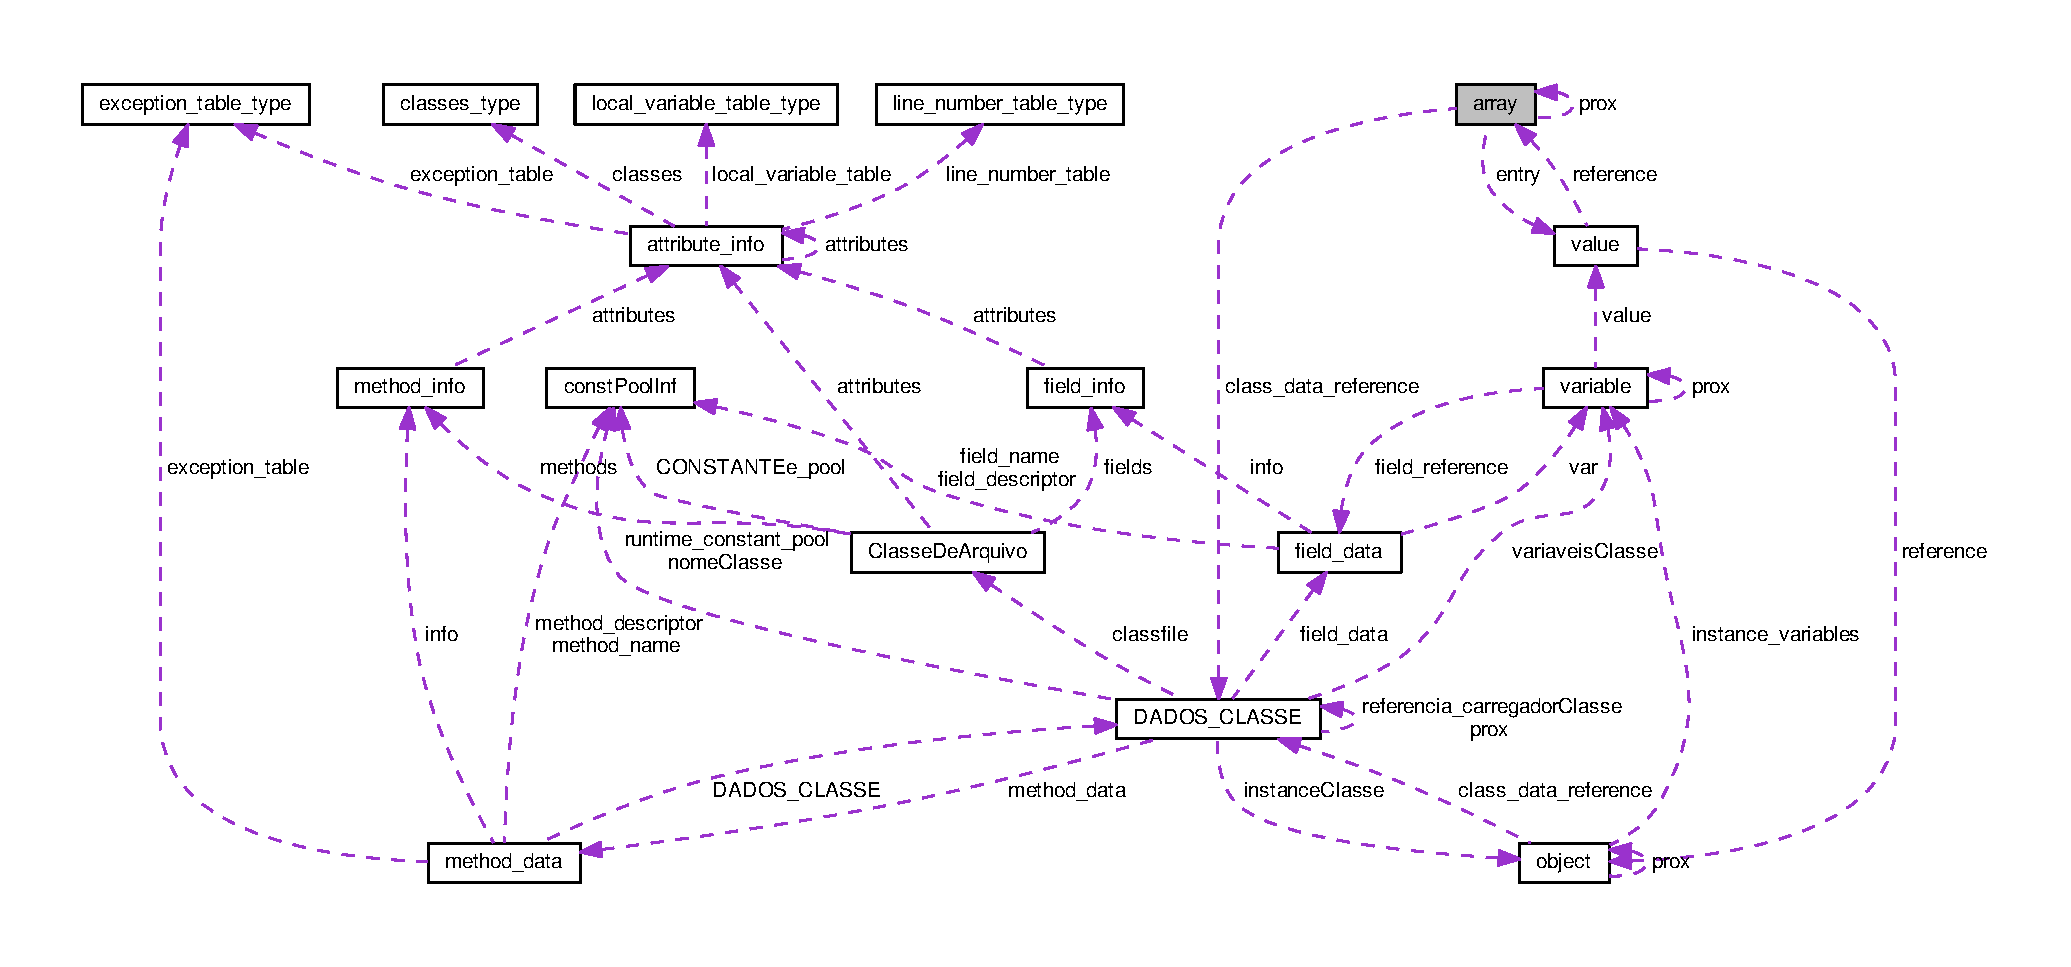
\includegraphics[width=350pt]{structarray__coll__graph}
\end{center}
\end{figure}
\subsection*{Atributos Públicos}
\begin{DoxyCompactItemize}
\item 
\hyperlink{struct_d_a_d_o_s___c_l_a_s_s_e}{D\-A\-D\-O\-S\-\_\-\-C\-L\-A\-S\-S\-E} $\ast$ \hyperlink{structarray_a48536838f6c8518606bb3ab53b8992c5}{class\-\_\-data\-\_\-reference}
\item 
int32\-\_\-t \hyperlink{structarray_ac87b36a4ba31b9d2a2bf77af4c136428}{count}
\item 
\hyperlink{core_8h_ad5d0e2bb91a9e28f920452e088b6462b}{V\-A\-L\-U\-E} $\ast$ \hyperlink{structarray_ae5d7e6555edc115b43c4595ab022023d}{entry}
\item 
\hyperlink{core_8h_aeeb4b41434914a6809f3448b40f818de}{A\-R\-R\-A\-Y\-\_\-\-T\-Y\-P\-E} \hyperlink{structarray_af7ebd5860861c4c445eea16d8385bee6}{atype}
\item 
struct \hyperlink{structarray}{array} $\ast$ \hyperlink{structarray_ac5278e82af38bcc76811769de4bd4400}{prox}
\end{DoxyCompactItemize}


\subsection{Descrição detalhada}


Definido na linha 176 do ficheiro core.\-h.



\subsection{Documentação dos dados membro}
\hypertarget{structarray_af7ebd5860861c4c445eea16d8385bee6}{\index{array@{array}!atype@{atype}}
\index{atype@{atype}!array@{array}}
\subsubsection[{atype}]{\setlength{\rightskip}{0pt plus 5cm}{\bf A\-R\-R\-A\-Y\-\_\-\-T\-Y\-P\-E} array\-::atype}}\label{structarray_af7ebd5860861c4c445eea16d8385bee6}


Definido na linha 180 do ficheiro core.\-h.

\hypertarget{structarray_a48536838f6c8518606bb3ab53b8992c5}{\index{array@{array}!class\-\_\-data\-\_\-reference@{class\-\_\-data\-\_\-reference}}
\index{class\-\_\-data\-\_\-reference@{class\-\_\-data\-\_\-reference}!array@{array}}
\subsubsection[{class\-\_\-data\-\_\-reference}]{\setlength{\rightskip}{0pt plus 5cm}{\bf D\-A\-D\-O\-S\-\_\-\-C\-L\-A\-S\-S\-E}$\ast$ array\-::class\-\_\-data\-\_\-reference}}\label{structarray_a48536838f6c8518606bb3ab53b8992c5}


Definido na linha 177 do ficheiro core.\-h.

\hypertarget{structarray_ac87b36a4ba31b9d2a2bf77af4c136428}{\index{array@{array}!count@{count}}
\index{count@{count}!array@{array}}
\subsubsection[{count}]{\setlength{\rightskip}{0pt plus 5cm}int32\-\_\-t array\-::count}}\label{structarray_ac87b36a4ba31b9d2a2bf77af4c136428}


Definido na linha 178 do ficheiro core.\-h.

\hypertarget{structarray_ae5d7e6555edc115b43c4595ab022023d}{\index{array@{array}!entry@{entry}}
\index{entry@{entry}!array@{array}}
\subsubsection[{entry}]{\setlength{\rightskip}{0pt plus 5cm}{\bf V\-A\-L\-U\-E}$\ast$ array\-::entry}}\label{structarray_ae5d7e6555edc115b43c4595ab022023d}


Definido na linha 179 do ficheiro core.\-h.

\hypertarget{structarray_ac5278e82af38bcc76811769de4bd4400}{\index{array@{array}!prox@{prox}}
\index{prox@{prox}!array@{array}}
\subsubsection[{prox}]{\setlength{\rightskip}{0pt plus 5cm}struct {\bf array}$\ast$ array\-::prox}}\label{structarray_ac5278e82af38bcc76811769de4bd4400}


Definido na linha 181 do ficheiro core.\-h.



A documentação para esta estrutura foi gerada a partir do seguinte ficheiro\-:\begin{DoxyCompactItemize}
\item 
\hyperlink{core_8h}{core.\-h}\end{DoxyCompactItemize}

\hypertarget{structattribute__info}{\section{Referência à estrutura attribute\-\_\-info}
\label{structattribute__info}\index{attribute\-\_\-info@{attribute\-\_\-info}}
}


{\ttfamily \#include $<$Leit\-Exib.\-h$>$}



Diagrama de colaboração para attribute\-\_\-info\-:\nopagebreak
\begin{figure}[H]
\begin{center}
\leavevmode
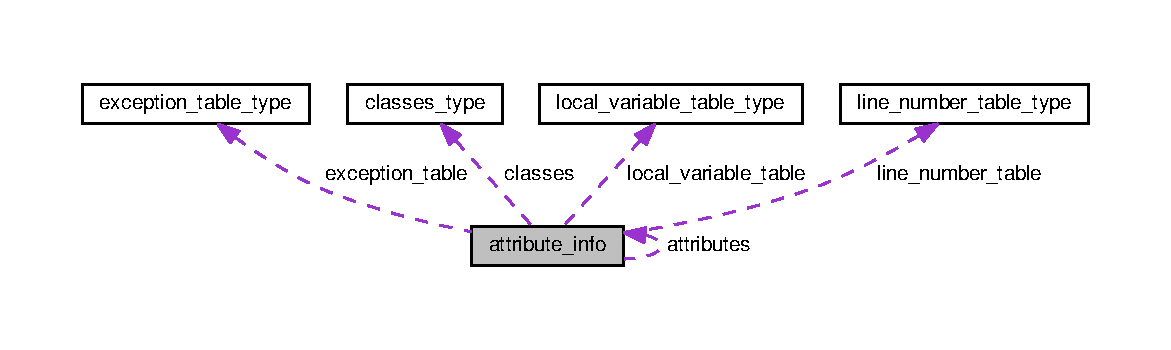
\includegraphics[width=350pt]{structattribute__info__coll__graph}
\end{center}
\end{figure}
\subsection*{Atributos Públicos}
\begin{DoxyCompactItemize}
\item 
uint16\-\_\-t \hyperlink{structattribute__info_aa8d580cb4c1e585270a11167bfdec6ff}{attribute\-\_\-name\-\_\-index}
\item 
uint32\-\_\-t \hyperlink{structattribute__info_a05bf4c6510e85d1adb7d75c2742b8550}{attribute\-\_\-length}
\item 
\begin{tabbing}
xx\=xx\=xx\=xx\=xx\=xx\=xx\=xx\=xx\=\kill
union \{\\
\>struct \{\\
\>\>uint16\_t \hyperlink{structattribute__info_aaf7c878962dc6671915725990a8152ef}{CONSTANTEvalue\_index}\\
\>\} \hyperlink{structattribute__info_ad720b5734bfd063b84a4348b4f246dd9}{CONSTANTEValue}\\
\>struct \{\\
\>\>uint16\_t \hyperlink{structattribute__info_ab617c25a5e4334c18cea3df9d2505c00}{max\_stack}\\
\>\>uint16\_t \hyperlink{structattribute__info_aa55aa7b42db88ca316e1bbe038b0dd16}{max\_locals}\\
\>\>uint32\_t \hyperlink{structattribute__info_afd6f0e0a9a7bac7c8c2173b5b278b329}{code\_length}\\
\>\>uint8\_t $\ast$ \hyperlink{structattribute__info_a15eebcb51490097313095ed5634767da}{code}\\
\>\>uint16\_t \hyperlink{structattribute__info_a6c6f8f7c78f29127b0e289c73516ddd7}{exception\_table\_length}\\
\>\>\hyperlink{structexception__table__type}{exception\_table\_type} $\ast$ \hyperlink{structattribute__info_aae0418a699927d0113442ad9f8b71dfc}{exception\_table}\\
\>\>uint16\_t \hyperlink{structattribute__info_add66058b51a906097b01d2f4695f4d9a}{conts\_atributos}\\
\>\>struct \hyperlink{structattribute__info}{attribute\_info} $\ast$ \hyperlink{structattribute__info_a405932cba2703fbf2ddc6487e3945108}{attributes}\\
\>\} \hyperlink{structattribute__info_a28164548bd28ed935b9e04966dac6651}{Code}\\
\>struct \{\\
\>\} \hyperlink{structattribute__info_ae4a470dfe9ebb19702f6b7f754f6c6af}{Deprecated}\\
\>struct \{\\
\>\>uint16\_t \hyperlink{structattribute__info_a7c0c2c58d833f7b63d0b6ab483e537f1}{number\_of\_exceptions}\\
\>\>uint16\_t $\ast$ \hyperlink{structattribute__info_a38178aee6eed0ea3d063727fed9cd100}{exception\_index\_table}\\
\>\} \hyperlink{structattribute__info_a4fc210f2d621b426637fb3a32e0783c0}{Exceptions}\\
\>struct \{\\
\>\>uint16\_t \hyperlink{structattribute__info_acf309770753a9a9e7cf0b91fb4dd45db}{number\_of\_classes}\\
\>\>\hyperlink{structclasses__type}{classes\_type} $\ast$ \hyperlink{structattribute__info_a65d85b8eb6a1f28360c9795ed98de13c}{classes}\\
\>\} \hyperlink{structattribute__info_a8b040beab0320ec8804cb3e640127a39}{InnerClasses}\\
\>struct \{\\
\>\>uint16\_t \hyperlink{structattribute__info_a81109c88e53b847e840ca2672b12700b}{line\_number\_table\_length}\\
\>\>\hyperlink{structline__number__table__type}{line\_number\_table\_type} $\ast$ \hyperlink{structattribute__info_aa4dba0207d2338202400c3860f5f6cbb}{line\_number\_table}\\
\>\} \hyperlink{structattribute__info_af6b14486315fa8c2d5b49b82e209c9aa}{LineNumberTable}\\
\>struct \{\\
\>\>uint16\_t \hyperlink{structattribute__info_a213dab40b46591df77874456f17d9282}{local\_variable\_table\_length}\\
\>\>\hyperlink{structlocal__variable__table__type}{local\_variable\_table\_type} $\ast$ \hyperlink{structattribute__info_aa3c58444ef5605c7dc24c82b3c76e7df}{local\_variable\_table}\\
\>\} \hyperlink{structattribute__info_a14fc812933da9d00004f2a85195ec991}{LocalVariableTable}\\
\>struct \{\\
\>\} \hyperlink{structattribute__info_a586a93df7c9a2b39e5b71d7b74817e78}{Synthetic}\\
\>struct \{\\
\>\>uint16\_t \hyperlink{structattribute__info_a9e5e8288eaa9f8649a0380fe8ae3056f}{sourcefile\_index}\\
\>\} \hyperlink{structattribute__info_a19be8f9c59a8338514cb47f8a654335d}{SourceFile}\\
\} \hyperlink{structattribute__info_ad6c58ccdd200eb05a9e2c1d34b624530}{u}\\

\end{tabbing}\end{DoxyCompactItemize}


\subsection{Descrição detalhada}


Definido na linha 164 do ficheiro Leit\-Exib.\-h.



\subsection{Documentação dos dados membro}
\hypertarget{structattribute__info_a05bf4c6510e85d1adb7d75c2742b8550}{\index{attribute\-\_\-info@{attribute\-\_\-info}!attribute\-\_\-length@{attribute\-\_\-length}}
\index{attribute\-\_\-length@{attribute\-\_\-length}!attribute_info@{attribute\-\_\-info}}
\subsubsection[{attribute\-\_\-length}]{\setlength{\rightskip}{0pt plus 5cm}uint32\-\_\-t attribute\-\_\-info\-::attribute\-\_\-length}}\label{structattribute__info_a05bf4c6510e85d1adb7d75c2742b8550}


Definido na linha 168 do ficheiro Leit\-Exib.\-h.

\hypertarget{structattribute__info_aa8d580cb4c1e585270a11167bfdec6ff}{\index{attribute\-\_\-info@{attribute\-\_\-info}!attribute\-\_\-name\-\_\-index@{attribute\-\_\-name\-\_\-index}}
\index{attribute\-\_\-name\-\_\-index@{attribute\-\_\-name\-\_\-index}!attribute_info@{attribute\-\_\-info}}
\subsubsection[{attribute\-\_\-name\-\_\-index}]{\setlength{\rightskip}{0pt plus 5cm}uint16\-\_\-t attribute\-\_\-info\-::attribute\-\_\-name\-\_\-index}}\label{structattribute__info_aa8d580cb4c1e585270a11167bfdec6ff}


Definido na linha 165 do ficheiro Leit\-Exib.\-h.

\hypertarget{structattribute__info_a405932cba2703fbf2ddc6487e3945108}{\index{attribute\-\_\-info@{attribute\-\_\-info}!attributes@{attributes}}
\index{attributes@{attributes}!attribute_info@{attribute\-\_\-info}}
\subsubsection[{attributes}]{\setlength{\rightskip}{0pt plus 5cm}struct {\bf attribute\-\_\-info}$\ast$ attribute\-\_\-info\-::attributes}}\label{structattribute__info_a405932cba2703fbf2ddc6487e3945108}


Definido na linha 182 do ficheiro Leit\-Exib.\-h.

\hypertarget{structattribute__info_a65d85b8eb6a1f28360c9795ed98de13c}{\index{attribute\-\_\-info@{attribute\-\_\-info}!classes@{classes}}
\index{classes@{classes}!attribute_info@{attribute\-\_\-info}}
\subsubsection[{classes}]{\setlength{\rightskip}{0pt plus 5cm}{\bf classes\-\_\-type}$\ast$ attribute\-\_\-info\-::classes}}\label{structattribute__info_a65d85b8eb6a1f28360c9795ed98de13c}


Definido na linha 195 do ficheiro Leit\-Exib.\-h.

\hypertarget{structattribute__info_a15eebcb51490097313095ed5634767da}{\index{attribute\-\_\-info@{attribute\-\_\-info}!code@{code}}
\index{code@{code}!attribute_info@{attribute\-\_\-info}}
\subsubsection[{code}]{\setlength{\rightskip}{0pt plus 5cm}uint8\-\_\-t$\ast$ attribute\-\_\-info\-::code}}\label{structattribute__info_a15eebcb51490097313095ed5634767da}


Definido na linha 178 do ficheiro Leit\-Exib.\-h.

\hypertarget{structattribute__info_a28164548bd28ed935b9e04966dac6651}{\index{attribute\-\_\-info@{attribute\-\_\-info}!Code@{Code}}
\index{Code@{Code}!attribute_info@{attribute\-\_\-info}}
\subsubsection[{Code}]{\setlength{\rightskip}{0pt plus 5cm}struct \{ ... \}   attribute\-\_\-info\-::\-Code}}\label{structattribute__info_a28164548bd28ed935b9e04966dac6651}
\hypertarget{structattribute__info_afd6f0e0a9a7bac7c8c2173b5b278b329}{\index{attribute\-\_\-info@{attribute\-\_\-info}!code\-\_\-length@{code\-\_\-length}}
\index{code\-\_\-length@{code\-\_\-length}!attribute_info@{attribute\-\_\-info}}
\subsubsection[{code\-\_\-length}]{\setlength{\rightskip}{0pt plus 5cm}uint32\-\_\-t attribute\-\_\-info\-::code\-\_\-length}}\label{structattribute__info_afd6f0e0a9a7bac7c8c2173b5b278b329}


Definido na linha 177 do ficheiro Leit\-Exib.\-h.

\hypertarget{structattribute__info_ad720b5734bfd063b84a4348b4f246dd9}{\index{attribute\-\_\-info@{attribute\-\_\-info}!C\-O\-N\-S\-T\-A\-N\-T\-E\-Value@{C\-O\-N\-S\-T\-A\-N\-T\-E\-Value}}
\index{C\-O\-N\-S\-T\-A\-N\-T\-E\-Value@{C\-O\-N\-S\-T\-A\-N\-T\-E\-Value}!attribute_info@{attribute\-\_\-info}}
\subsubsection[{C\-O\-N\-S\-T\-A\-N\-T\-E\-Value}]{\setlength{\rightskip}{0pt plus 5cm}struct \{ ... \}   attribute\-\_\-info\-::\-C\-O\-N\-S\-T\-A\-N\-T\-E\-Value}}\label{structattribute__info_ad720b5734bfd063b84a4348b4f246dd9}
\hypertarget{structattribute__info_aaf7c878962dc6671915725990a8152ef}{\index{attribute\-\_\-info@{attribute\-\_\-info}!C\-O\-N\-S\-T\-A\-N\-T\-Evalue\-\_\-index@{C\-O\-N\-S\-T\-A\-N\-T\-Evalue\-\_\-index}}
\index{C\-O\-N\-S\-T\-A\-N\-T\-Evalue\-\_\-index@{C\-O\-N\-S\-T\-A\-N\-T\-Evalue\-\_\-index}!attribute_info@{attribute\-\_\-info}}
\subsubsection[{C\-O\-N\-S\-T\-A\-N\-T\-Evalue\-\_\-index}]{\setlength{\rightskip}{0pt plus 5cm}uint16\-\_\-t attribute\-\_\-info\-::\-C\-O\-N\-S\-T\-A\-N\-T\-Evalue\-\_\-index}}\label{structattribute__info_aaf7c878962dc6671915725990a8152ef}


Definido na linha 171 do ficheiro Leit\-Exib.\-h.

\hypertarget{structattribute__info_add66058b51a906097b01d2f4695f4d9a}{\index{attribute\-\_\-info@{attribute\-\_\-info}!conts\-\_\-atributos@{conts\-\_\-atributos}}
\index{conts\-\_\-atributos@{conts\-\_\-atributos}!attribute_info@{attribute\-\_\-info}}
\subsubsection[{conts\-\_\-atributos}]{\setlength{\rightskip}{0pt plus 5cm}uint16\-\_\-t attribute\-\_\-info\-::conts\-\_\-atributos}}\label{structattribute__info_add66058b51a906097b01d2f4695f4d9a}


Definido na linha 181 do ficheiro Leit\-Exib.\-h.

\hypertarget{structattribute__info_ae4a470dfe9ebb19702f6b7f754f6c6af}{\index{attribute\-\_\-info@{attribute\-\_\-info}!Deprecated@{Deprecated}}
\index{Deprecated@{Deprecated}!attribute_info@{attribute\-\_\-info}}
\subsubsection[{Deprecated}]{\setlength{\rightskip}{0pt plus 5cm}struct \{ ... \}   attribute\-\_\-info\-::\-Deprecated}}\label{structattribute__info_ae4a470dfe9ebb19702f6b7f754f6c6af}
\hypertarget{structattribute__info_a38178aee6eed0ea3d063727fed9cd100}{\index{attribute\-\_\-info@{attribute\-\_\-info}!exception\-\_\-index\-\_\-table@{exception\-\_\-index\-\_\-table}}
\index{exception\-\_\-index\-\_\-table@{exception\-\_\-index\-\_\-table}!attribute_info@{attribute\-\_\-info}}
\subsubsection[{exception\-\_\-index\-\_\-table}]{\setlength{\rightskip}{0pt plus 5cm}uint16\-\_\-t$\ast$ attribute\-\_\-info\-::exception\-\_\-index\-\_\-table}}\label{structattribute__info_a38178aee6eed0ea3d063727fed9cd100}


Definido na linha 190 do ficheiro Leit\-Exib.\-h.

\hypertarget{structattribute__info_aae0418a699927d0113442ad9f8b71dfc}{\index{attribute\-\_\-info@{attribute\-\_\-info}!exception\-\_\-table@{exception\-\_\-table}}
\index{exception\-\_\-table@{exception\-\_\-table}!attribute_info@{attribute\-\_\-info}}
\subsubsection[{exception\-\_\-table}]{\setlength{\rightskip}{0pt plus 5cm}{\bf exception\-\_\-table\-\_\-type}$\ast$ attribute\-\_\-info\-::exception\-\_\-table}}\label{structattribute__info_aae0418a699927d0113442ad9f8b71dfc}


Definido na linha 180 do ficheiro Leit\-Exib.\-h.

\hypertarget{structattribute__info_a6c6f8f7c78f29127b0e289c73516ddd7}{\index{attribute\-\_\-info@{attribute\-\_\-info}!exception\-\_\-table\-\_\-length@{exception\-\_\-table\-\_\-length}}
\index{exception\-\_\-table\-\_\-length@{exception\-\_\-table\-\_\-length}!attribute_info@{attribute\-\_\-info}}
\subsubsection[{exception\-\_\-table\-\_\-length}]{\setlength{\rightskip}{0pt plus 5cm}uint16\-\_\-t attribute\-\_\-info\-::exception\-\_\-table\-\_\-length}}\label{structattribute__info_a6c6f8f7c78f29127b0e289c73516ddd7}


Definido na linha 179 do ficheiro Leit\-Exib.\-h.

\hypertarget{structattribute__info_a4fc210f2d621b426637fb3a32e0783c0}{\index{attribute\-\_\-info@{attribute\-\_\-info}!Exceptions@{Exceptions}}
\index{Exceptions@{Exceptions}!attribute_info@{attribute\-\_\-info}}
\subsubsection[{Exceptions}]{\setlength{\rightskip}{0pt plus 5cm}struct \{ ... \}   attribute\-\_\-info\-::\-Exceptions}}\label{structattribute__info_a4fc210f2d621b426637fb3a32e0783c0}
\hypertarget{structattribute__info_a8b040beab0320ec8804cb3e640127a39}{\index{attribute\-\_\-info@{attribute\-\_\-info}!Inner\-Classes@{Inner\-Classes}}
\index{Inner\-Classes@{Inner\-Classes}!attribute_info@{attribute\-\_\-info}}
\subsubsection[{Inner\-Classes}]{\setlength{\rightskip}{0pt plus 5cm}struct \{ ... \}   attribute\-\_\-info\-::\-Inner\-Classes}}\label{structattribute__info_a8b040beab0320ec8804cb3e640127a39}
\hypertarget{structattribute__info_aa4dba0207d2338202400c3860f5f6cbb}{\index{attribute\-\_\-info@{attribute\-\_\-info}!line\-\_\-number\-\_\-table@{line\-\_\-number\-\_\-table}}
\index{line\-\_\-number\-\_\-table@{line\-\_\-number\-\_\-table}!attribute_info@{attribute\-\_\-info}}
\subsubsection[{line\-\_\-number\-\_\-table}]{\setlength{\rightskip}{0pt plus 5cm}{\bf line\-\_\-number\-\_\-table\-\_\-type}$\ast$ attribute\-\_\-info\-::line\-\_\-number\-\_\-table}}\label{structattribute__info_aa4dba0207d2338202400c3860f5f6cbb}


Definido na linha 200 do ficheiro Leit\-Exib.\-h.

\hypertarget{structattribute__info_a81109c88e53b847e840ca2672b12700b}{\index{attribute\-\_\-info@{attribute\-\_\-info}!line\-\_\-number\-\_\-table\-\_\-length@{line\-\_\-number\-\_\-table\-\_\-length}}
\index{line\-\_\-number\-\_\-table\-\_\-length@{line\-\_\-number\-\_\-table\-\_\-length}!attribute_info@{attribute\-\_\-info}}
\subsubsection[{line\-\_\-number\-\_\-table\-\_\-length}]{\setlength{\rightskip}{0pt plus 5cm}uint16\-\_\-t attribute\-\_\-info\-::line\-\_\-number\-\_\-table\-\_\-length}}\label{structattribute__info_a81109c88e53b847e840ca2672b12700b}


Definido na linha 199 do ficheiro Leit\-Exib.\-h.

\hypertarget{structattribute__info_af6b14486315fa8c2d5b49b82e209c9aa}{\index{attribute\-\_\-info@{attribute\-\_\-info}!Line\-Number\-Table@{Line\-Number\-Table}}
\index{Line\-Number\-Table@{Line\-Number\-Table}!attribute_info@{attribute\-\_\-info}}
\subsubsection[{Line\-Number\-Table}]{\setlength{\rightskip}{0pt plus 5cm}struct \{ ... \}   attribute\-\_\-info\-::\-Line\-Number\-Table}}\label{structattribute__info_af6b14486315fa8c2d5b49b82e209c9aa}
\hypertarget{structattribute__info_aa3c58444ef5605c7dc24c82b3c76e7df}{\index{attribute\-\_\-info@{attribute\-\_\-info}!local\-\_\-variable\-\_\-table@{local\-\_\-variable\-\_\-table}}
\index{local\-\_\-variable\-\_\-table@{local\-\_\-variable\-\_\-table}!attribute_info@{attribute\-\_\-info}}
\subsubsection[{local\-\_\-variable\-\_\-table}]{\setlength{\rightskip}{0pt plus 5cm}{\bf local\-\_\-variable\-\_\-table\-\_\-type}$\ast$ attribute\-\_\-info\-::local\-\_\-variable\-\_\-table}}\label{structattribute__info_aa3c58444ef5605c7dc24c82b3c76e7df}


Definido na linha 205 do ficheiro Leit\-Exib.\-h.

\hypertarget{structattribute__info_a213dab40b46591df77874456f17d9282}{\index{attribute\-\_\-info@{attribute\-\_\-info}!local\-\_\-variable\-\_\-table\-\_\-length@{local\-\_\-variable\-\_\-table\-\_\-length}}
\index{local\-\_\-variable\-\_\-table\-\_\-length@{local\-\_\-variable\-\_\-table\-\_\-length}!attribute_info@{attribute\-\_\-info}}
\subsubsection[{local\-\_\-variable\-\_\-table\-\_\-length}]{\setlength{\rightskip}{0pt plus 5cm}uint16\-\_\-t attribute\-\_\-info\-::local\-\_\-variable\-\_\-table\-\_\-length}}\label{structattribute__info_a213dab40b46591df77874456f17d9282}


Definido na linha 204 do ficheiro Leit\-Exib.\-h.

\hypertarget{structattribute__info_a14fc812933da9d00004f2a85195ec991}{\index{attribute\-\_\-info@{attribute\-\_\-info}!Local\-Variable\-Table@{Local\-Variable\-Table}}
\index{Local\-Variable\-Table@{Local\-Variable\-Table}!attribute_info@{attribute\-\_\-info}}
\subsubsection[{Local\-Variable\-Table}]{\setlength{\rightskip}{0pt plus 5cm}struct \{ ... \}   attribute\-\_\-info\-::\-Local\-Variable\-Table}}\label{structattribute__info_a14fc812933da9d00004f2a85195ec991}
\hypertarget{structattribute__info_aa55aa7b42db88ca316e1bbe038b0dd16}{\index{attribute\-\_\-info@{attribute\-\_\-info}!max\-\_\-locals@{max\-\_\-locals}}
\index{max\-\_\-locals@{max\-\_\-locals}!attribute_info@{attribute\-\_\-info}}
\subsubsection[{max\-\_\-locals}]{\setlength{\rightskip}{0pt plus 5cm}uint16\-\_\-t attribute\-\_\-info\-::max\-\_\-locals}}\label{structattribute__info_aa55aa7b42db88ca316e1bbe038b0dd16}


Definido na linha 176 do ficheiro Leit\-Exib.\-h.

\hypertarget{structattribute__info_ab617c25a5e4334c18cea3df9d2505c00}{\index{attribute\-\_\-info@{attribute\-\_\-info}!max\-\_\-stack@{max\-\_\-stack}}
\index{max\-\_\-stack@{max\-\_\-stack}!attribute_info@{attribute\-\_\-info}}
\subsubsection[{max\-\_\-stack}]{\setlength{\rightskip}{0pt plus 5cm}uint16\-\_\-t attribute\-\_\-info\-::max\-\_\-stack}}\label{structattribute__info_ab617c25a5e4334c18cea3df9d2505c00}


Definido na linha 175 do ficheiro Leit\-Exib.\-h.

\hypertarget{structattribute__info_acf309770753a9a9e7cf0b91fb4dd45db}{\index{attribute\-\_\-info@{attribute\-\_\-info}!number\-\_\-of\-\_\-classes@{number\-\_\-of\-\_\-classes}}
\index{number\-\_\-of\-\_\-classes@{number\-\_\-of\-\_\-classes}!attribute_info@{attribute\-\_\-info}}
\subsubsection[{number\-\_\-of\-\_\-classes}]{\setlength{\rightskip}{0pt plus 5cm}uint16\-\_\-t attribute\-\_\-info\-::number\-\_\-of\-\_\-classes}}\label{structattribute__info_acf309770753a9a9e7cf0b91fb4dd45db}


Definido na linha 194 do ficheiro Leit\-Exib.\-h.

\hypertarget{structattribute__info_a7c0c2c58d833f7b63d0b6ab483e537f1}{\index{attribute\-\_\-info@{attribute\-\_\-info}!number\-\_\-of\-\_\-exceptions@{number\-\_\-of\-\_\-exceptions}}
\index{number\-\_\-of\-\_\-exceptions@{number\-\_\-of\-\_\-exceptions}!attribute_info@{attribute\-\_\-info}}
\subsubsection[{number\-\_\-of\-\_\-exceptions}]{\setlength{\rightskip}{0pt plus 5cm}uint16\-\_\-t attribute\-\_\-info\-::number\-\_\-of\-\_\-exceptions}}\label{structattribute__info_a7c0c2c58d833f7b63d0b6ab483e537f1}


Definido na linha 189 do ficheiro Leit\-Exib.\-h.

\hypertarget{structattribute__info_a19be8f9c59a8338514cb47f8a654335d}{\index{attribute\-\_\-info@{attribute\-\_\-info}!Source\-File@{Source\-File}}
\index{Source\-File@{Source\-File}!attribute_info@{attribute\-\_\-info}}
\subsubsection[{Source\-File}]{\setlength{\rightskip}{0pt plus 5cm}struct \{ ... \}   attribute\-\_\-info\-::\-Source\-File}}\label{structattribute__info_a19be8f9c59a8338514cb47f8a654335d}
\hypertarget{structattribute__info_a9e5e8288eaa9f8649a0380fe8ae3056f}{\index{attribute\-\_\-info@{attribute\-\_\-info}!sourcefile\-\_\-index@{sourcefile\-\_\-index}}
\index{sourcefile\-\_\-index@{sourcefile\-\_\-index}!attribute_info@{attribute\-\_\-info}}
\subsubsection[{sourcefile\-\_\-index}]{\setlength{\rightskip}{0pt plus 5cm}uint16\-\_\-t attribute\-\_\-info\-::sourcefile\-\_\-index}}\label{structattribute__info_a9e5e8288eaa9f8649a0380fe8ae3056f}


Definido na linha 212 do ficheiro Leit\-Exib.\-h.

\hypertarget{structattribute__info_a586a93df7c9a2b39e5b71d7b74817e78}{\index{attribute\-\_\-info@{attribute\-\_\-info}!Synthetic@{Synthetic}}
\index{Synthetic@{Synthetic}!attribute_info@{attribute\-\_\-info}}
\subsubsection[{Synthetic}]{\setlength{\rightskip}{0pt plus 5cm}struct \{ ... \}   attribute\-\_\-info\-::\-Synthetic}}\label{structattribute__info_a586a93df7c9a2b39e5b71d7b74817e78}
\hypertarget{structattribute__info_ad6c58ccdd200eb05a9e2c1d34b624530}{\index{attribute\-\_\-info@{attribute\-\_\-info}!u@{u}}
\index{u@{u}!attribute_info@{attribute\-\_\-info}}
\subsubsection[{u}]{\setlength{\rightskip}{0pt plus 5cm}union \{ ... \}   attribute\-\_\-info\-::u}}\label{structattribute__info_ad6c58ccdd200eb05a9e2c1d34b624530}


A documentação para esta estrutura foi gerada a partir do seguinte ficheiro\-:\begin{DoxyCompactItemize}
\item 
\hyperlink{_leit_exib_8h}{Leit\-Exib.\-h}\end{DoxyCompactItemize}

\hypertarget{struct_classe_de_arquivo}{\section{Referência à estrutura Classe\-De\-Arquivo}
\label{struct_classe_de_arquivo}\index{Classe\-De\-Arquivo@{Classe\-De\-Arquivo}}
}


{\ttfamily \#include $<$Leit\-Exib.\-h$>$}



Diagrama de colaboração para Classe\-De\-Arquivo\-:\nopagebreak
\begin{figure}[H]
\begin{center}
\leavevmode
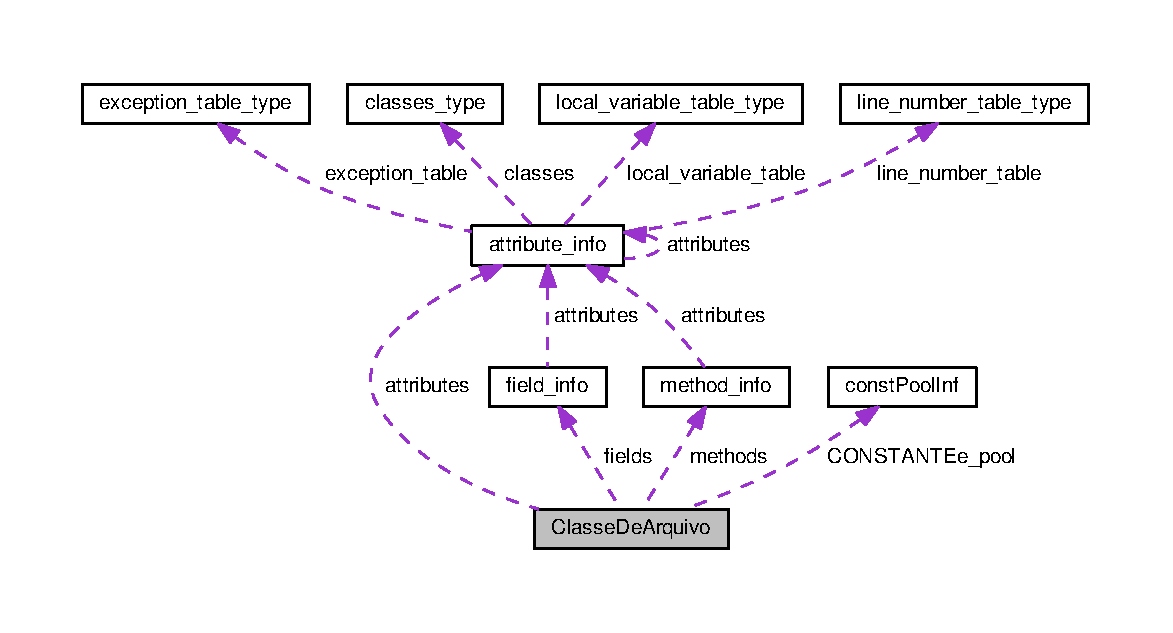
\includegraphics[width=350pt]{struct_classe_de_arquivo__coll__graph}
\end{center}
\end{figure}
\subsection*{Atributos Públicos}
\begin{DoxyCompactItemize}
\item 
uint32\-\_\-t \hyperlink{struct_classe_de_arquivo_a57331bb82cd19880ff79226bb2432fae}{magic}
\item 
uint16\-\_\-t \hyperlink{struct_classe_de_arquivo_a1a97a970253c7f8651cf450a5dbc98a7}{Min\-\_\-version}
\item 
uint16\-\_\-t \hyperlink{struct_classe_de_arquivo_a6f45d7c9f0026ebf84d4c83c46fcc547}{Principal\-\_\-version}
\item 
uint16\-\_\-t \hyperlink{struct_classe_de_arquivo_a86527645a99cde472e6ae443aaff7b4e}{Cont\-\_\-\-Const\-Pool}
\item 
\hyperlink{structconst_pool_inf}{const\-Pool\-Inf} $\ast$ \hyperlink{struct_classe_de_arquivo_a41c0d5758a7188709f83876e9577e134}{C\-O\-N\-S\-T\-A\-N\-T\-Ee\-\_\-pool}
\item 
uint16\-\_\-t \hyperlink{struct_classe_de_arquivo_a113235ae98d51c48780e11d39debf99f}{flags\-\_\-acesso}
\item 
uint16\-\_\-t \hyperlink{struct_classe_de_arquivo_ace786690df6e3ea741a18e3b49102e2b}{classe\-\_\-arq}
\item 
uint16\-\_\-t \hyperlink{struct_classe_de_arquivo_a250195b0cd2dfc88bf912da18aa9d558}{super\-\_\-classe}
\item 
uint16\-\_\-t \hyperlink{struct_classe_de_arquivo_a81969140a877d9eb2eda7616c58e2a4d}{interfaces\-\_\-count}
\item 
uint16\-\_\-t $\ast$ \hyperlink{struct_classe_de_arquivo_a7ab7e89f230794a963028b0e827ef878}{interfaces}
\item 
uint16\-\_\-t \hyperlink{struct_classe_de_arquivo_a11ed358daa97442f5d1e16f5acf4fbcc}{conts\-\_\-campos}
\item 
\hyperlink{structfield__info}{field\-\_\-info} $\ast$ \hyperlink{struct_classe_de_arquivo_a0a756640d8c9a35fb2068e4da70b0f9a}{fields}
\item 
uint16\-\_\-t \hyperlink{struct_classe_de_arquivo_a51e6aee87a53ffaec03f9fde63b33f35}{conts\-\_\-metodo}
\item 
\hyperlink{structmethod__info}{method\-\_\-info} $\ast$ \hyperlink{struct_classe_de_arquivo_a2b6a999458d5759967527d26a3219450}{methods}
\item 
uint16\-\_\-t \hyperlink{struct_classe_de_arquivo_aedc3f8105d268a28a6a02b39b28f8ddd}{conts\-\_\-atributos}
\item 
\hyperlink{structattribute__info}{attribute\-\_\-info} $\ast$ \hyperlink{struct_classe_de_arquivo_a9119e38492ee3cba2075867129584f66}{attributes}
\end{DoxyCompactItemize}


\subsection{Descrição detalhada}


Definido na linha 245 do ficheiro Leit\-Exib.\-h.



\subsection{Documentação dos dados membro}
\hypertarget{struct_classe_de_arquivo_a9119e38492ee3cba2075867129584f66}{\index{Classe\-De\-Arquivo@{Classe\-De\-Arquivo}!attributes@{attributes}}
\index{attributes@{attributes}!ClasseDeArquivo@{Classe\-De\-Arquivo}}
\subsubsection[{attributes}]{\setlength{\rightskip}{0pt plus 5cm}{\bf attribute\-\_\-info}$\ast$ Classe\-De\-Arquivo\-::attributes}}\label{struct_classe_de_arquivo_a9119e38492ee3cba2075867129584f66}


Definido na linha 290 do ficheiro Leit\-Exib.\-h.

\hypertarget{struct_classe_de_arquivo_ace786690df6e3ea741a18e3b49102e2b}{\index{Classe\-De\-Arquivo@{Classe\-De\-Arquivo}!classe\-\_\-arq@{classe\-\_\-arq}}
\index{classe\-\_\-arq@{classe\-\_\-arq}!ClasseDeArquivo@{Classe\-De\-Arquivo}}
\subsubsection[{classe\-\_\-arq}]{\setlength{\rightskip}{0pt plus 5cm}uint16\-\_\-t Classe\-De\-Arquivo\-::classe\-\_\-arq}}\label{struct_classe_de_arquivo_ace786690df6e3ea741a18e3b49102e2b}


Definido na linha 267 do ficheiro Leit\-Exib.\-h.

\hypertarget{struct_classe_de_arquivo_a41c0d5758a7188709f83876e9577e134}{\index{Classe\-De\-Arquivo@{Classe\-De\-Arquivo}!C\-O\-N\-S\-T\-A\-N\-T\-Ee\-\_\-pool@{C\-O\-N\-S\-T\-A\-N\-T\-Ee\-\_\-pool}}
\index{C\-O\-N\-S\-T\-A\-N\-T\-Ee\-\_\-pool@{C\-O\-N\-S\-T\-A\-N\-T\-Ee\-\_\-pool}!ClasseDeArquivo@{Classe\-De\-Arquivo}}
\subsubsection[{C\-O\-N\-S\-T\-A\-N\-T\-Ee\-\_\-pool}]{\setlength{\rightskip}{0pt plus 5cm}{\bf const\-Pool\-Inf}$\ast$ Classe\-De\-Arquivo\-::\-C\-O\-N\-S\-T\-A\-N\-T\-Ee\-\_\-pool}}\label{struct_classe_de_arquivo_a41c0d5758a7188709f83876e9577e134}


Definido na linha 259 do ficheiro Leit\-Exib.\-h.

\hypertarget{struct_classe_de_arquivo_a86527645a99cde472e6ae443aaff7b4e}{\index{Classe\-De\-Arquivo@{Classe\-De\-Arquivo}!Cont\-\_\-\-Const\-Pool@{Cont\-\_\-\-Const\-Pool}}
\index{Cont\-\_\-\-Const\-Pool@{Cont\-\_\-\-Const\-Pool}!ClasseDeArquivo@{Classe\-De\-Arquivo}}
\subsubsection[{Cont\-\_\-\-Const\-Pool}]{\setlength{\rightskip}{0pt plus 5cm}uint16\-\_\-t Classe\-De\-Arquivo\-::\-Cont\-\_\-\-Const\-Pool}}\label{struct_classe_de_arquivo_a86527645a99cde472e6ae443aaff7b4e}


Definido na linha 253 do ficheiro Leit\-Exib.\-h.

\hypertarget{struct_classe_de_arquivo_aedc3f8105d268a28a6a02b39b28f8ddd}{\index{Classe\-De\-Arquivo@{Classe\-De\-Arquivo}!conts\-\_\-atributos@{conts\-\_\-atributos}}
\index{conts\-\_\-atributos@{conts\-\_\-atributos}!ClasseDeArquivo@{Classe\-De\-Arquivo}}
\subsubsection[{conts\-\_\-atributos}]{\setlength{\rightskip}{0pt plus 5cm}uint16\-\_\-t Classe\-De\-Arquivo\-::conts\-\_\-atributos}}\label{struct_classe_de_arquivo_aedc3f8105d268a28a6a02b39b28f8ddd}


Definido na linha 289 do ficheiro Leit\-Exib.\-h.

\hypertarget{struct_classe_de_arquivo_a11ed358daa97442f5d1e16f5acf4fbcc}{\index{Classe\-De\-Arquivo@{Classe\-De\-Arquivo}!conts\-\_\-campos@{conts\-\_\-campos}}
\index{conts\-\_\-campos@{conts\-\_\-campos}!ClasseDeArquivo@{Classe\-De\-Arquivo}}
\subsubsection[{conts\-\_\-campos}]{\setlength{\rightskip}{0pt plus 5cm}uint16\-\_\-t Classe\-De\-Arquivo\-::conts\-\_\-campos}}\label{struct_classe_de_arquivo_a11ed358daa97442f5d1e16f5acf4fbcc}


Definido na linha 279 do ficheiro Leit\-Exib.\-h.

\hypertarget{struct_classe_de_arquivo_a51e6aee87a53ffaec03f9fde63b33f35}{\index{Classe\-De\-Arquivo@{Classe\-De\-Arquivo}!conts\-\_\-metodo@{conts\-\_\-metodo}}
\index{conts\-\_\-metodo@{conts\-\_\-metodo}!ClasseDeArquivo@{Classe\-De\-Arquivo}}
\subsubsection[{conts\-\_\-metodo}]{\setlength{\rightskip}{0pt plus 5cm}uint16\-\_\-t Classe\-De\-Arquivo\-::conts\-\_\-metodo}}\label{struct_classe_de_arquivo_a51e6aee87a53ffaec03f9fde63b33f35}


Definido na linha 284 do ficheiro Leit\-Exib.\-h.

\hypertarget{struct_classe_de_arquivo_a0a756640d8c9a35fb2068e4da70b0f9a}{\index{Classe\-De\-Arquivo@{Classe\-De\-Arquivo}!fields@{fields}}
\index{fields@{fields}!ClasseDeArquivo@{Classe\-De\-Arquivo}}
\subsubsection[{fields}]{\setlength{\rightskip}{0pt plus 5cm}{\bf field\-\_\-info}$\ast$ Classe\-De\-Arquivo\-::fields}}\label{struct_classe_de_arquivo_a0a756640d8c9a35fb2068e4da70b0f9a}


Definido na linha 280 do ficheiro Leit\-Exib.\-h.

\hypertarget{struct_classe_de_arquivo_a113235ae98d51c48780e11d39debf99f}{\index{Classe\-De\-Arquivo@{Classe\-De\-Arquivo}!flags\-\_\-acesso@{flags\-\_\-acesso}}
\index{flags\-\_\-acesso@{flags\-\_\-acesso}!ClasseDeArquivo@{Classe\-De\-Arquivo}}
\subsubsection[{flags\-\_\-acesso}]{\setlength{\rightskip}{0pt plus 5cm}uint16\-\_\-t Classe\-De\-Arquivo\-::flags\-\_\-acesso}}\label{struct_classe_de_arquivo_a113235ae98d51c48780e11d39debf99f}


Definido na linha 263 do ficheiro Leit\-Exib.\-h.

\hypertarget{struct_classe_de_arquivo_a7ab7e89f230794a963028b0e827ef878}{\index{Classe\-De\-Arquivo@{Classe\-De\-Arquivo}!interfaces@{interfaces}}
\index{interfaces@{interfaces}!ClasseDeArquivo@{Classe\-De\-Arquivo}}
\subsubsection[{interfaces}]{\setlength{\rightskip}{0pt plus 5cm}uint16\-\_\-t$\ast$ Classe\-De\-Arquivo\-::interfaces}}\label{struct_classe_de_arquivo_a7ab7e89f230794a963028b0e827ef878}


Definido na linha 274 do ficheiro Leit\-Exib.\-h.

\hypertarget{struct_classe_de_arquivo_a81969140a877d9eb2eda7616c58e2a4d}{\index{Classe\-De\-Arquivo@{Classe\-De\-Arquivo}!interfaces\-\_\-count@{interfaces\-\_\-count}}
\index{interfaces\-\_\-count@{interfaces\-\_\-count}!ClasseDeArquivo@{Classe\-De\-Arquivo}}
\subsubsection[{interfaces\-\_\-count}]{\setlength{\rightskip}{0pt plus 5cm}uint16\-\_\-t Classe\-De\-Arquivo\-::interfaces\-\_\-count}}\label{struct_classe_de_arquivo_a81969140a877d9eb2eda7616c58e2a4d}


Definido na linha 273 do ficheiro Leit\-Exib.\-h.

\hypertarget{struct_classe_de_arquivo_a57331bb82cd19880ff79226bb2432fae}{\index{Classe\-De\-Arquivo@{Classe\-De\-Arquivo}!magic@{magic}}
\index{magic@{magic}!ClasseDeArquivo@{Classe\-De\-Arquivo}}
\subsubsection[{magic}]{\setlength{\rightskip}{0pt plus 5cm}uint32\-\_\-t Classe\-De\-Arquivo\-::magic}}\label{struct_classe_de_arquivo_a57331bb82cd19880ff79226bb2432fae}


Definido na linha 246 do ficheiro Leit\-Exib.\-h.

\hypertarget{struct_classe_de_arquivo_a2b6a999458d5759967527d26a3219450}{\index{Classe\-De\-Arquivo@{Classe\-De\-Arquivo}!methods@{methods}}
\index{methods@{methods}!ClasseDeArquivo@{Classe\-De\-Arquivo}}
\subsubsection[{methods}]{\setlength{\rightskip}{0pt plus 5cm}{\bf method\-\_\-info}$\ast$ Classe\-De\-Arquivo\-::methods}}\label{struct_classe_de_arquivo_a2b6a999458d5759967527d26a3219450}


Definido na linha 285 do ficheiro Leit\-Exib.\-h.

\hypertarget{struct_classe_de_arquivo_a1a97a970253c7f8651cf450a5dbc98a7}{\index{Classe\-De\-Arquivo@{Classe\-De\-Arquivo}!Min\-\_\-version@{Min\-\_\-version}}
\index{Min\-\_\-version@{Min\-\_\-version}!ClasseDeArquivo@{Classe\-De\-Arquivo}}
\subsubsection[{Min\-\_\-version}]{\setlength{\rightskip}{0pt plus 5cm}uint16\-\_\-t Classe\-De\-Arquivo\-::\-Min\-\_\-version}}\label{struct_classe_de_arquivo_a1a97a970253c7f8651cf450a5dbc98a7}


Definido na linha 248 do ficheiro Leit\-Exib.\-h.

\hypertarget{struct_classe_de_arquivo_a6f45d7c9f0026ebf84d4c83c46fcc547}{\index{Classe\-De\-Arquivo@{Classe\-De\-Arquivo}!Principal\-\_\-version@{Principal\-\_\-version}}
\index{Principal\-\_\-version@{Principal\-\_\-version}!ClasseDeArquivo@{Classe\-De\-Arquivo}}
\subsubsection[{Principal\-\_\-version}]{\setlength{\rightskip}{0pt plus 5cm}uint16\-\_\-t Classe\-De\-Arquivo\-::\-Principal\-\_\-version}}\label{struct_classe_de_arquivo_a6f45d7c9f0026ebf84d4c83c46fcc547}


Definido na linha 249 do ficheiro Leit\-Exib.\-h.

\hypertarget{struct_classe_de_arquivo_a250195b0cd2dfc88bf912da18aa9d558}{\index{Classe\-De\-Arquivo@{Classe\-De\-Arquivo}!super\-\_\-classe@{super\-\_\-classe}}
\index{super\-\_\-classe@{super\-\_\-classe}!ClasseDeArquivo@{Classe\-De\-Arquivo}}
\subsubsection[{super\-\_\-classe}]{\setlength{\rightskip}{0pt plus 5cm}uint16\-\_\-t Classe\-De\-Arquivo\-::super\-\_\-classe}}\label{struct_classe_de_arquivo_a250195b0cd2dfc88bf912da18aa9d558}


Definido na linha 270 do ficheiro Leit\-Exib.\-h.



A documentação para esta estrutura foi gerada a partir do seguinte ficheiro\-:\begin{DoxyCompactItemize}
\item 
\hyperlink{_leit_exib_8h}{Leit\-Exib.\-h}\end{DoxyCompactItemize}

\hypertarget{structclasses__type}{\section{Referência à estrutura classes\-\_\-type}
\label{structclasses__type}\index{classes\-\_\-type@{classes\-\_\-type}}
}


{\ttfamily \#include $<$Leit\-Exib.\-h$>$}

\subsection*{Atributos Públicos}
\begin{DoxyCompactItemize}
\item 
uint16\-\_\-t \hyperlink{structclasses__type_a8ee3c154b6031adfa97fccc80d7a76ff}{inner\-\_\-class\-\_\-info\-\_\-index}
\item 
uint16\-\_\-t \hyperlink{structclasses__type_a8a32528b616cd9d1cfc3278e8c942f8f}{outer\-\_\-class\-\_\-info\-\_\-index}
\item 
uint16\-\_\-t \hyperlink{structclasses__type_acd3c408b30a72b1ae22a56fb8642684c}{inner\-\_\-name\-\_\-index}
\item 
uint16\-\_\-t \hyperlink{structclasses__type_a6e2e0b5e77749572a331f070924620ad}{inner\-\_\-class\-\_\-access\-\_\-flags}
\end{DoxyCompactItemize}


\subsection{Descrição detalhada}


Definido na linha 143 do ficheiro Leit\-Exib.\-h.



\subsection{Documentação dos dados membro}
\hypertarget{structclasses__type_a6e2e0b5e77749572a331f070924620ad}{\index{classes\-\_\-type@{classes\-\_\-type}!inner\-\_\-class\-\_\-access\-\_\-flags@{inner\-\_\-class\-\_\-access\-\_\-flags}}
\index{inner\-\_\-class\-\_\-access\-\_\-flags@{inner\-\_\-class\-\_\-access\-\_\-flags}!classes_type@{classes\-\_\-type}}
\subsubsection[{inner\-\_\-class\-\_\-access\-\_\-flags}]{\setlength{\rightskip}{0pt plus 5cm}uint16\-\_\-t classes\-\_\-type\-::inner\-\_\-class\-\_\-access\-\_\-flags}}\label{structclasses__type_a6e2e0b5e77749572a331f070924620ad}


Definido na linha 147 do ficheiro Leit\-Exib.\-h.

\hypertarget{structclasses__type_a8ee3c154b6031adfa97fccc80d7a76ff}{\index{classes\-\_\-type@{classes\-\_\-type}!inner\-\_\-class\-\_\-info\-\_\-index@{inner\-\_\-class\-\_\-info\-\_\-index}}
\index{inner\-\_\-class\-\_\-info\-\_\-index@{inner\-\_\-class\-\_\-info\-\_\-index}!classes_type@{classes\-\_\-type}}
\subsubsection[{inner\-\_\-class\-\_\-info\-\_\-index}]{\setlength{\rightskip}{0pt plus 5cm}uint16\-\_\-t classes\-\_\-type\-::inner\-\_\-class\-\_\-info\-\_\-index}}\label{structclasses__type_a8ee3c154b6031adfa97fccc80d7a76ff}


Definido na linha 144 do ficheiro Leit\-Exib.\-h.

\hypertarget{structclasses__type_acd3c408b30a72b1ae22a56fb8642684c}{\index{classes\-\_\-type@{classes\-\_\-type}!inner\-\_\-name\-\_\-index@{inner\-\_\-name\-\_\-index}}
\index{inner\-\_\-name\-\_\-index@{inner\-\_\-name\-\_\-index}!classes_type@{classes\-\_\-type}}
\subsubsection[{inner\-\_\-name\-\_\-index}]{\setlength{\rightskip}{0pt plus 5cm}uint16\-\_\-t classes\-\_\-type\-::inner\-\_\-name\-\_\-index}}\label{structclasses__type_acd3c408b30a72b1ae22a56fb8642684c}


Definido na linha 146 do ficheiro Leit\-Exib.\-h.

\hypertarget{structclasses__type_a8a32528b616cd9d1cfc3278e8c942f8f}{\index{classes\-\_\-type@{classes\-\_\-type}!outer\-\_\-class\-\_\-info\-\_\-index@{outer\-\_\-class\-\_\-info\-\_\-index}}
\index{outer\-\_\-class\-\_\-info\-\_\-index@{outer\-\_\-class\-\_\-info\-\_\-index}!classes_type@{classes\-\_\-type}}
\subsubsection[{outer\-\_\-class\-\_\-info\-\_\-index}]{\setlength{\rightskip}{0pt plus 5cm}uint16\-\_\-t classes\-\_\-type\-::outer\-\_\-class\-\_\-info\-\_\-index}}\label{structclasses__type_a8a32528b616cd9d1cfc3278e8c942f8f}


Definido na linha 145 do ficheiro Leit\-Exib.\-h.



A documentação para esta estrutura foi gerada a partir do seguinte ficheiro\-:\begin{DoxyCompactItemize}
\item 
\hyperlink{_leit_exib_8h}{Leit\-Exib.\-h}\end{DoxyCompactItemize}

\hypertarget{structconst_pool_inf}{\section{Referência à estrutura const\-Pool\-Inf}
\label{structconst_pool_inf}\index{const\-Pool\-Inf@{const\-Pool\-Inf}}
}


{\ttfamily \#include $<$Leit\-Exib.\-h$>$}

\subsection*{Atributos Públicos}
\begin{DoxyCompactItemize}
\item 
uint8\-\_\-t \hyperlink{structconst_pool_inf_a6ea639ac2bd081a75fb00ee2231b5bf3}{tag}
\item 
\begin{tabbing}
xx\=xx\=xx\=xx\=xx\=xx\=xx\=xx\=xx\=\kill
union \{\\
\>struct \{\\
\>\>uint16\_t \hyperlink{structconst_pool_inf_a2f80c7393ff5829654d7418b7264110a}{indicador\_nome}\\
\>\} \hyperlink{structconst_pool_inf_adb4639fcbfae6547548f36dac46a1ce5}{Class}\\
\>struct \{\\
\>\>uint16\_t \hyperlink{structconst_pool_inf_a2f80c7393ff5829654d7418b7264110a}{indicador\_nome}\\
\>\>uint16\_t \hyperlink{structconst_pool_inf_adcd281157000a467608ba65cf1a6efb6}{indicador\_nome\_e\_tipo}\\
\>\} \hyperlink{structconst_pool_inf_ad0c502e47bccc75b8e939e5ccd1a8a16}{Ref}\\
\>struct \{\\
\>\>uint16\_t \hyperlink{structconst_pool_inf_a2f80c7393ff5829654d7418b7264110a}{indicador\_nome}\\
\>\>uint16\_t \hyperlink{structconst_pool_inf_a01d1f403e7ed5762b986ae2fe6e7db4b}{descriptor\_index}\\
\>\} \hyperlink{structconst_pool_inf_addb54edaecbb6a09ef4799c98134332a}{NameAndType}\\
\>struct \{\\
\>\>uint16\_t \hyperlink{structconst_pool_inf_a3c4be7f5456b58187d9695bb1d3c8871}{length}\\
\>\>uint8\_t $\ast$ \hyperlink{structconst_pool_inf_ad855f3fa643b42a9f2506f06d2f74310}{bytes}\\
\>\} \hyperlink{structconst_pool_inf_abf7874c7fbecc53ed38466b1ff897746}{Utf8}\\
\>struct \{\\
\>\>uint16\_t \hyperlink{structconst_pool_inf_a0d09a4566d526db83cd87836f18df28c}{indicador\_string}\\
\>\} \hyperlink{structconst_pool_inf_adfd1e8831065142d9deb97e7bd79c356}{String}\\
\>struct \{\\
\>\>uint32\_t \hyperlink{structconst_pool_inf_a6e7de138b8c2f5514813538787f73c16}{bytes}\\
\>\} \hyperlink{structconst_pool_inf_a9cc60d2e41859cb617704d61374ddb74}{Integer\_Float}\\
\>struct \{\\
\>\>uint32\_t \hyperlink{structconst_pool_inf_ab116ef79f6cae5784e038805c26f2d20}{high\_bytes}\\
\>\>uint32\_t \hyperlink{structconst_pool_inf_a15471799757777098756cc8ec1cd9a3c}{low\_bytes}\\
\>\} \hyperlink{structconst_pool_inf_a25e99a2c4f18168165ed83b5f4cfe234}{Long\_Double}\\
\} \hyperlink{structconst_pool_inf_ad39a609c73e52b6faa7d2f1a29a14d28}{u}\\

\end{tabbing}\end{DoxyCompactItemize}


\subsection{Descrição detalhada}


Definido na linha 98 do ficheiro Leit\-Exib.\-h.



\subsection{Documentação dos dados membro}
\hypertarget{structconst_pool_inf_ad855f3fa643b42a9f2506f06d2f74310}{\index{const\-Pool\-Inf@{const\-Pool\-Inf}!bytes@{bytes}}
\index{bytes@{bytes}!constPoolInf@{const\-Pool\-Inf}}
\subsubsection[{bytes}]{\setlength{\rightskip}{0pt plus 5cm}uint8\-\_\-t$\ast$ const\-Pool\-Inf\-::bytes}}\label{structconst_pool_inf_ad855f3fa643b42a9f2506f06d2f74310}


Definido na linha 117 do ficheiro Leit\-Exib.\-h.

\hypertarget{structconst_pool_inf_a6e7de138b8c2f5514813538787f73c16}{\index{const\-Pool\-Inf@{const\-Pool\-Inf}!bytes@{bytes}}
\index{bytes@{bytes}!constPoolInf@{const\-Pool\-Inf}}
\subsubsection[{bytes}]{\setlength{\rightskip}{0pt plus 5cm}uint32\-\_\-t const\-Pool\-Inf\-::bytes}}\label{structconst_pool_inf_a6e7de138b8c2f5514813538787f73c16}


Definido na linha 125 do ficheiro Leit\-Exib.\-h.

\hypertarget{structconst_pool_inf_adb4639fcbfae6547548f36dac46a1ce5}{\index{const\-Pool\-Inf@{const\-Pool\-Inf}!Class@{Class}}
\index{Class@{Class}!constPoolInf@{const\-Pool\-Inf}}
\subsubsection[{Class}]{\setlength{\rightskip}{0pt plus 5cm}struct \{ ... \}   const\-Pool\-Inf\-::\-Class}}\label{structconst_pool_inf_adb4639fcbfae6547548f36dac46a1ce5}
\hypertarget{structconst_pool_inf_a01d1f403e7ed5762b986ae2fe6e7db4b}{\index{const\-Pool\-Inf@{const\-Pool\-Inf}!descriptor\-\_\-index@{descriptor\-\_\-index}}
\index{descriptor\-\_\-index@{descriptor\-\_\-index}!constPoolInf@{const\-Pool\-Inf}}
\subsubsection[{descriptor\-\_\-index}]{\setlength{\rightskip}{0pt plus 5cm}uint16\-\_\-t const\-Pool\-Inf\-::descriptor\-\_\-index}}\label{structconst_pool_inf_a01d1f403e7ed5762b986ae2fe6e7db4b}


Definido na linha 112 do ficheiro Leit\-Exib.\-h.

\hypertarget{structconst_pool_inf_ab116ef79f6cae5784e038805c26f2d20}{\index{const\-Pool\-Inf@{const\-Pool\-Inf}!high\-\_\-bytes@{high\-\_\-bytes}}
\index{high\-\_\-bytes@{high\-\_\-bytes}!constPoolInf@{const\-Pool\-Inf}}
\subsubsection[{high\-\_\-bytes}]{\setlength{\rightskip}{0pt plus 5cm}uint32\-\_\-t const\-Pool\-Inf\-::high\-\_\-bytes}}\label{structconst_pool_inf_ab116ef79f6cae5784e038805c26f2d20}


Definido na linha 129 do ficheiro Leit\-Exib.\-h.

\hypertarget{structconst_pool_inf_a2f80c7393ff5829654d7418b7264110a}{\index{const\-Pool\-Inf@{const\-Pool\-Inf}!indicador\-\_\-nome@{indicador\-\_\-nome}}
\index{indicador\-\_\-nome@{indicador\-\_\-nome}!constPoolInf@{const\-Pool\-Inf}}
\subsubsection[{indicador\-\_\-nome}]{\setlength{\rightskip}{0pt plus 5cm}uint16\-\_\-t const\-Pool\-Inf\-::indicador\-\_\-nome}}\label{structconst_pool_inf_a2f80c7393ff5829654d7418b7264110a}


Definido na linha 102 do ficheiro Leit\-Exib.\-h.

\hypertarget{structconst_pool_inf_adcd281157000a467608ba65cf1a6efb6}{\index{const\-Pool\-Inf@{const\-Pool\-Inf}!indicador\-\_\-nome\-\_\-e\-\_\-tipo@{indicador\-\_\-nome\-\_\-e\-\_\-tipo}}
\index{indicador\-\_\-nome\-\_\-e\-\_\-tipo@{indicador\-\_\-nome\-\_\-e\-\_\-tipo}!constPoolInf@{const\-Pool\-Inf}}
\subsubsection[{indicador\-\_\-nome\-\_\-e\-\_\-tipo}]{\setlength{\rightskip}{0pt plus 5cm}uint16\-\_\-t const\-Pool\-Inf\-::indicador\-\_\-nome\-\_\-e\-\_\-tipo}}\label{structconst_pool_inf_adcd281157000a467608ba65cf1a6efb6}


Definido na linha 107 do ficheiro Leit\-Exib.\-h.

\hypertarget{structconst_pool_inf_a0d09a4566d526db83cd87836f18df28c}{\index{const\-Pool\-Inf@{const\-Pool\-Inf}!indicador\-\_\-string@{indicador\-\_\-string}}
\index{indicador\-\_\-string@{indicador\-\_\-string}!constPoolInf@{const\-Pool\-Inf}}
\subsubsection[{indicador\-\_\-string}]{\setlength{\rightskip}{0pt plus 5cm}uint16\-\_\-t const\-Pool\-Inf\-::indicador\-\_\-string}}\label{structconst_pool_inf_a0d09a4566d526db83cd87836f18df28c}


Definido na linha 121 do ficheiro Leit\-Exib.\-h.

\hypertarget{structconst_pool_inf_a9cc60d2e41859cb617704d61374ddb74}{\index{const\-Pool\-Inf@{const\-Pool\-Inf}!Integer\-\_\-\-Float@{Integer\-\_\-\-Float}}
\index{Integer\-\_\-\-Float@{Integer\-\_\-\-Float}!constPoolInf@{const\-Pool\-Inf}}
\subsubsection[{Integer\-\_\-\-Float}]{\setlength{\rightskip}{0pt plus 5cm}struct \{ ... \}   const\-Pool\-Inf\-::\-Integer\-\_\-\-Float}}\label{structconst_pool_inf_a9cc60d2e41859cb617704d61374ddb74}
\hypertarget{structconst_pool_inf_a3c4be7f5456b58187d9695bb1d3c8871}{\index{const\-Pool\-Inf@{const\-Pool\-Inf}!length@{length}}
\index{length@{length}!constPoolInf@{const\-Pool\-Inf}}
\subsubsection[{length}]{\setlength{\rightskip}{0pt plus 5cm}uint16\-\_\-t const\-Pool\-Inf\-::length}}\label{structconst_pool_inf_a3c4be7f5456b58187d9695bb1d3c8871}


Definido na linha 116 do ficheiro Leit\-Exib.\-h.

\hypertarget{structconst_pool_inf_a25e99a2c4f18168165ed83b5f4cfe234}{\index{const\-Pool\-Inf@{const\-Pool\-Inf}!Long\-\_\-\-Double@{Long\-\_\-\-Double}}
\index{Long\-\_\-\-Double@{Long\-\_\-\-Double}!constPoolInf@{const\-Pool\-Inf}}
\subsubsection[{Long\-\_\-\-Double}]{\setlength{\rightskip}{0pt plus 5cm}struct \{ ... \}   const\-Pool\-Inf\-::\-Long\-\_\-\-Double}}\label{structconst_pool_inf_a25e99a2c4f18168165ed83b5f4cfe234}
\hypertarget{structconst_pool_inf_a15471799757777098756cc8ec1cd9a3c}{\index{const\-Pool\-Inf@{const\-Pool\-Inf}!low\-\_\-bytes@{low\-\_\-bytes}}
\index{low\-\_\-bytes@{low\-\_\-bytes}!constPoolInf@{const\-Pool\-Inf}}
\subsubsection[{low\-\_\-bytes}]{\setlength{\rightskip}{0pt plus 5cm}uint32\-\_\-t const\-Pool\-Inf\-::low\-\_\-bytes}}\label{structconst_pool_inf_a15471799757777098756cc8ec1cd9a3c}


Definido na linha 130 do ficheiro Leit\-Exib.\-h.

\hypertarget{structconst_pool_inf_addb54edaecbb6a09ef4799c98134332a}{\index{const\-Pool\-Inf@{const\-Pool\-Inf}!Name\-And\-Type@{Name\-And\-Type}}
\index{Name\-And\-Type@{Name\-And\-Type}!constPoolInf@{const\-Pool\-Inf}}
\subsubsection[{Name\-And\-Type}]{\setlength{\rightskip}{0pt plus 5cm}struct \{ ... \}   const\-Pool\-Inf\-::\-Name\-And\-Type}}\label{structconst_pool_inf_addb54edaecbb6a09ef4799c98134332a}
\hypertarget{structconst_pool_inf_ad0c502e47bccc75b8e939e5ccd1a8a16}{\index{const\-Pool\-Inf@{const\-Pool\-Inf}!Ref@{Ref}}
\index{Ref@{Ref}!constPoolInf@{const\-Pool\-Inf}}
\subsubsection[{Ref}]{\setlength{\rightskip}{0pt plus 5cm}struct \{ ... \}   const\-Pool\-Inf\-::\-Ref}}\label{structconst_pool_inf_ad0c502e47bccc75b8e939e5ccd1a8a16}
\hypertarget{structconst_pool_inf_adfd1e8831065142d9deb97e7bd79c356}{\index{const\-Pool\-Inf@{const\-Pool\-Inf}!String@{String}}
\index{String@{String}!constPoolInf@{const\-Pool\-Inf}}
\subsubsection[{String}]{\setlength{\rightskip}{0pt plus 5cm}struct \{ ... \}   const\-Pool\-Inf\-::\-String}}\label{structconst_pool_inf_adfd1e8831065142d9deb97e7bd79c356}
\hypertarget{structconst_pool_inf_a6ea639ac2bd081a75fb00ee2231b5bf3}{\index{const\-Pool\-Inf@{const\-Pool\-Inf}!tag@{tag}}
\index{tag@{tag}!constPoolInf@{const\-Pool\-Inf}}
\subsubsection[{tag}]{\setlength{\rightskip}{0pt plus 5cm}uint8\-\_\-t const\-Pool\-Inf\-::tag}}\label{structconst_pool_inf_a6ea639ac2bd081a75fb00ee2231b5bf3}


Definido na linha 99 do ficheiro Leit\-Exib.\-h.

\hypertarget{structconst_pool_inf_ad39a609c73e52b6faa7d2f1a29a14d28}{\index{const\-Pool\-Inf@{const\-Pool\-Inf}!u@{u}}
\index{u@{u}!constPoolInf@{const\-Pool\-Inf}}
\subsubsection[{u}]{\setlength{\rightskip}{0pt plus 5cm}union \{ ... \}   const\-Pool\-Inf\-::u}}\label{structconst_pool_inf_ad39a609c73e52b6faa7d2f1a29a14d28}
\hypertarget{structconst_pool_inf_abf7874c7fbecc53ed38466b1ff897746}{\index{const\-Pool\-Inf@{const\-Pool\-Inf}!Utf8@{Utf8}}
\index{Utf8@{Utf8}!constPoolInf@{const\-Pool\-Inf}}
\subsubsection[{Utf8}]{\setlength{\rightskip}{0pt plus 5cm}struct \{ ... \}   const\-Pool\-Inf\-::\-Utf8}}\label{structconst_pool_inf_abf7874c7fbecc53ed38466b1ff897746}


A documentação para esta estrutura foi gerada a partir do seguinte ficheiro\-:\begin{DoxyCompactItemize}
\item 
\hyperlink{_leit_exib_8h}{Leit\-Exib.\-h}\end{DoxyCompactItemize}

\hypertarget{struct_d_a_d_o_s___c_l_a_s_s_e}{\section{Referência à estrutura D\-A\-D\-O\-S\-\_\-\-C\-L\-A\-S\-S\-E}
\label{struct_d_a_d_o_s___c_l_a_s_s_e}\index{D\-A\-D\-O\-S\-\_\-\-C\-L\-A\-S\-S\-E@{D\-A\-D\-O\-S\-\_\-\-C\-L\-A\-S\-S\-E}}
}


{\ttfamily \#include $<$core.\-h$>$}



Diagrama de colaboração para D\-A\-D\-O\-S\-\_\-\-C\-L\-A\-S\-S\-E\-:\nopagebreak
\begin{figure}[H]
\begin{center}
\leavevmode
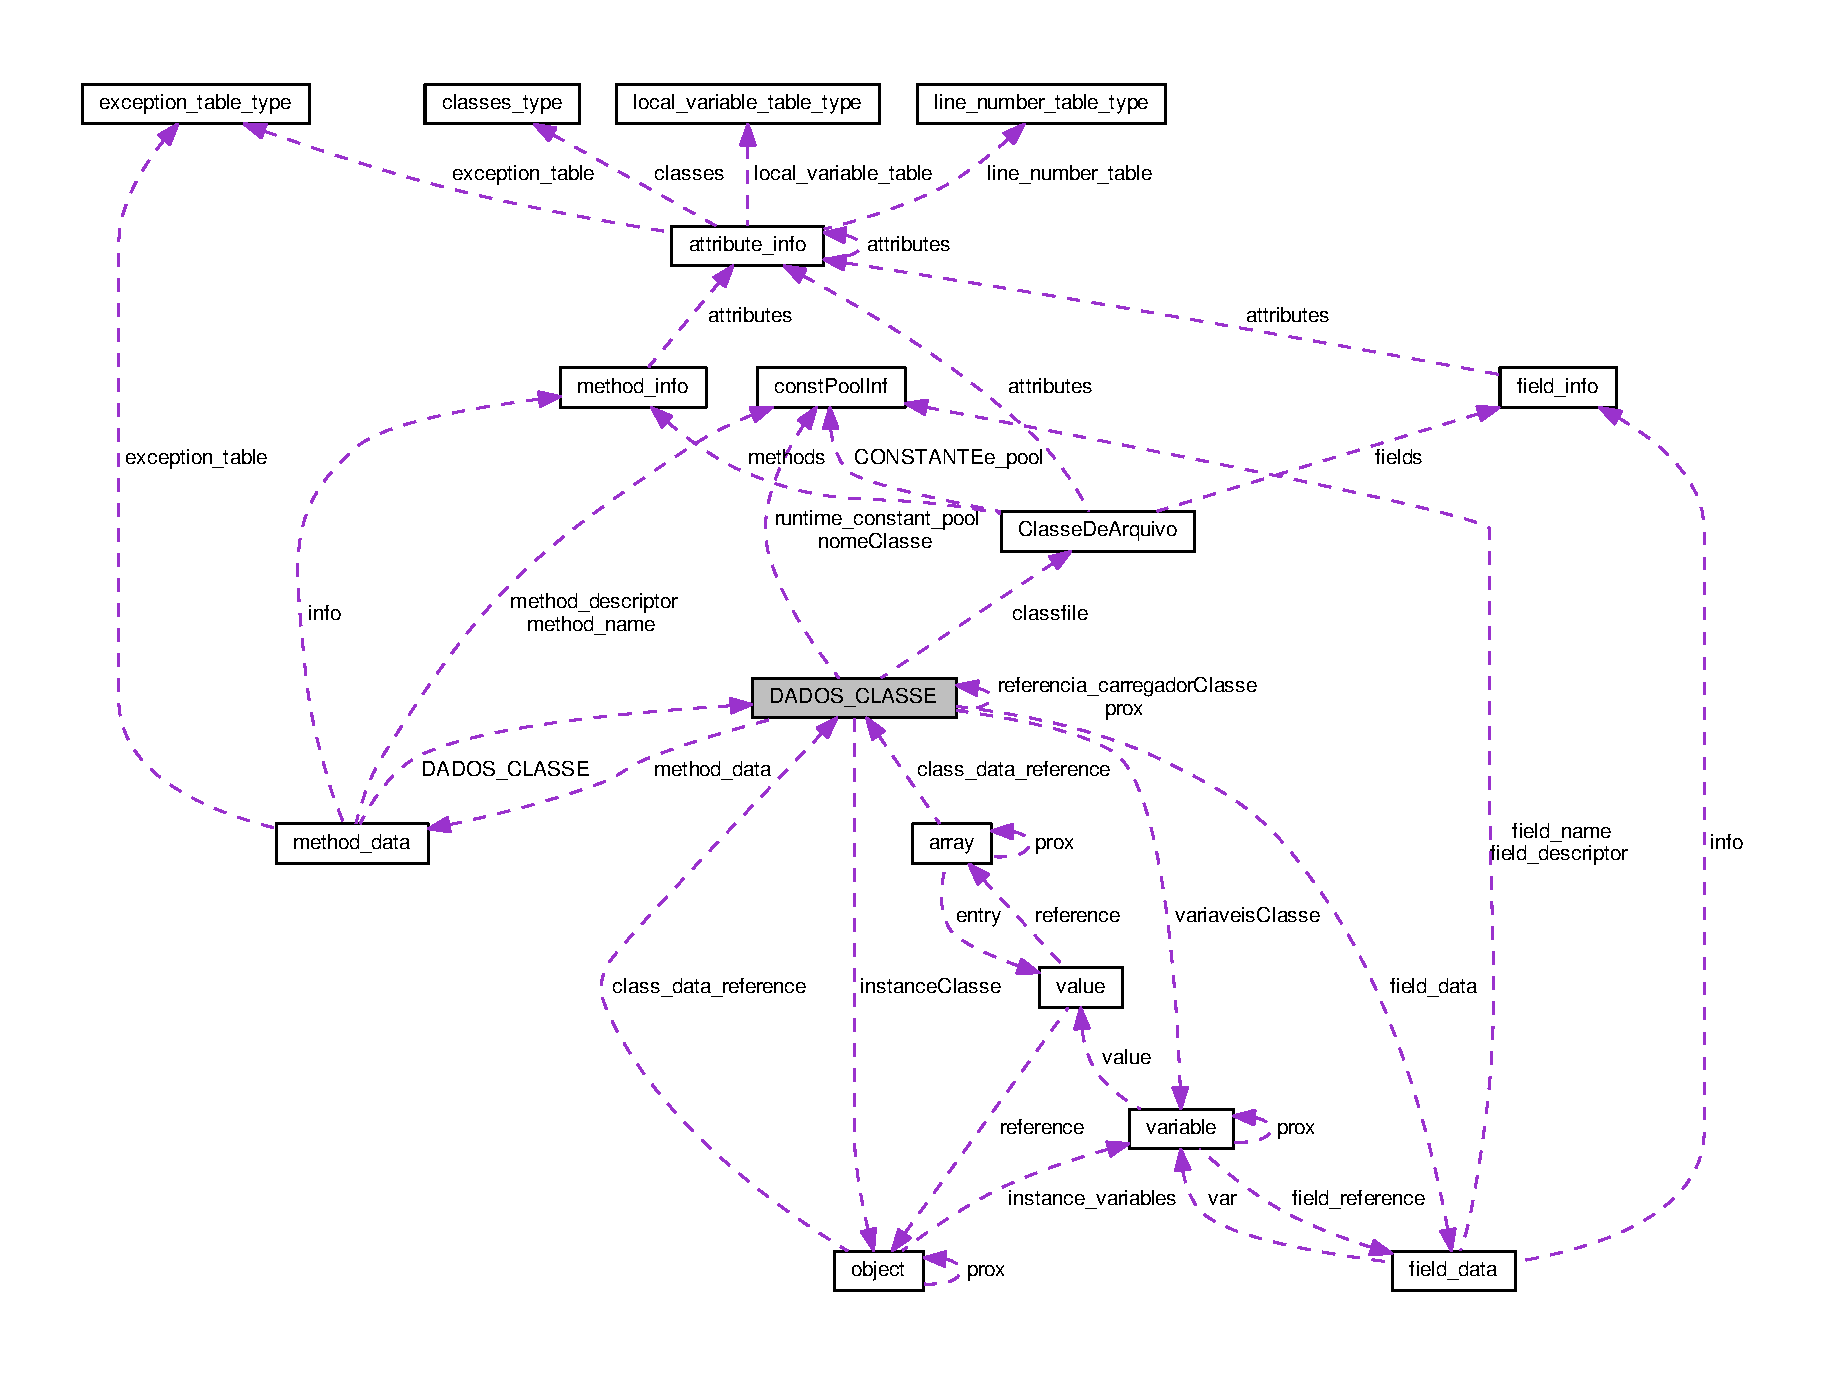
\includegraphics[width=350pt]{struct_d_a_d_o_s___c_l_a_s_s_e__coll__graph}
\end{center}
\end{figure}
\subsection*{Atributos Públicos}
\begin{DoxyCompactItemize}
\item 
\hyperlink{structconst_pool_inf}{const\-Pool\-Inf} $\ast$ \hyperlink{struct_d_a_d_o_s___c_l_a_s_s_e_aa36d42ba9b426675415d1da6c02e4420}{nome\-Classe}
\item 
\hyperlink{struct_classe_de_arquivo}{Classe\-De\-Arquivo} $\ast$ \hyperlink{struct_d_a_d_o_s___c_l_a_s_s_e_a04a5c6ada8a199cc0f66130e8f3fd0db}{classfile}
\item 
uint16\-\_\-t \hyperlink{struct_d_a_d_o_s___c_l_a_s_s_e_a49b8ef228c1e9116fa30acb28a3b6402}{modifiers}
\item 
struct \hyperlink{struct_d_a_d_o_s___c_l_a_s_s_e}{D\-A\-D\-O\-S\-\_\-\-C\-L\-A\-S\-S\-E} $\ast$ \hyperlink{struct_d_a_d_o_s___c_l_a_s_s_e_af50666164c0a79d63ff831010e8318c9}{referencia\-\_\-carregador\-Classe}
\item 
\hyperlink{structconst_pool_inf}{const\-Pool\-Inf} $\ast$ \hyperlink{struct_d_a_d_o_s___c_l_a_s_s_e_a0c018490460fc694fc1bcdeddbd49e02}{runtime\-\_\-constant\-\_\-pool}
\item 
\hyperlink{core_8h_ad5537b62ac62d6b7f34e2303f2b84982}{F\-I\-E\-L\-D\-\_\-\-D\-A\-T\-A} $\ast$ \hyperlink{struct_d_a_d_o_s___c_l_a_s_s_e_a6a524c5e2a3eda5b548ee3cf703c727d}{field\-\_\-data}
\item 
\hyperlink{core_8h_af2592f49e52b0675aaca5850571f3999}{M\-E\-T\-H\-O\-D\-\_\-\-D\-A\-T\-A} $\ast$ \hyperlink{struct_d_a_d_o_s___c_l_a_s_s_e_a75c522131e8a7325da50f22f8c373ffa}{method\-\_\-data}
\item 
\hyperlink{core_8h_a85b40991452ad00efae1784148c94402}{V\-A\-R\-I\-A\-B\-L\-E} $\ast$ \hyperlink{struct_d_a_d_o_s___c_l_a_s_s_e_a61814affa4242c9de4ab4380163ae315}{variaveis\-Classe}
\item 
struct \hyperlink{structobject}{object} $\ast$ \hyperlink{struct_d_a_d_o_s___c_l_a_s_s_e_a3e8be397f59bd8130a2d3df976af3830}{instance\-Classe}
\item 
struct \hyperlink{struct_d_a_d_o_s___c_l_a_s_s_e}{D\-A\-D\-O\-S\-\_\-\-C\-L\-A\-S\-S\-E} $\ast$ \hyperlink{struct_d_a_d_o_s___c_l_a_s_s_e_a5d3d779158876f9def507bdad79037be}{prox}
\end{DoxyCompactItemize}


\subsection{Descrição detalhada}


Definido na linha 157 do ficheiro core.\-h.



\subsection{Documentação dos dados membro}
\hypertarget{struct_d_a_d_o_s___c_l_a_s_s_e_a04a5c6ada8a199cc0f66130e8f3fd0db}{\index{D\-A\-D\-O\-S\-\_\-\-C\-L\-A\-S\-S\-E@{D\-A\-D\-O\-S\-\_\-\-C\-L\-A\-S\-S\-E}!classfile@{classfile}}
\index{classfile@{classfile}!DADOS_CLASSE@{D\-A\-D\-O\-S\-\_\-\-C\-L\-A\-S\-S\-E}}
\subsubsection[{classfile}]{\setlength{\rightskip}{0pt plus 5cm}{\bf Classe\-De\-Arquivo}$\ast$ D\-A\-D\-O\-S\-\_\-\-C\-L\-A\-S\-S\-E\-::classfile}}\label{struct_d_a_d_o_s___c_l_a_s_s_e_a04a5c6ada8a199cc0f66130e8f3fd0db}


Definido na linha 159 do ficheiro core.\-h.

\hypertarget{struct_d_a_d_o_s___c_l_a_s_s_e_a6a524c5e2a3eda5b548ee3cf703c727d}{\index{D\-A\-D\-O\-S\-\_\-\-C\-L\-A\-S\-S\-E@{D\-A\-D\-O\-S\-\_\-\-C\-L\-A\-S\-S\-E}!field\-\_\-data@{field\-\_\-data}}
\index{field\-\_\-data@{field\-\_\-data}!DADOS_CLASSE@{D\-A\-D\-O\-S\-\_\-\-C\-L\-A\-S\-S\-E}}
\subsubsection[{field\-\_\-data}]{\setlength{\rightskip}{0pt plus 5cm}{\bf F\-I\-E\-L\-D\-\_\-\-D\-A\-T\-A}$\ast$ D\-A\-D\-O\-S\-\_\-\-C\-L\-A\-S\-S\-E\-::field\-\_\-data}}\label{struct_d_a_d_o_s___c_l_a_s_s_e_a6a524c5e2a3eda5b548ee3cf703c727d}


Definido na linha 163 do ficheiro core.\-h.

\hypertarget{struct_d_a_d_o_s___c_l_a_s_s_e_a3e8be397f59bd8130a2d3df976af3830}{\index{D\-A\-D\-O\-S\-\_\-\-C\-L\-A\-S\-S\-E@{D\-A\-D\-O\-S\-\_\-\-C\-L\-A\-S\-S\-E}!instance\-Classe@{instance\-Classe}}
\index{instance\-Classe@{instance\-Classe}!DADOS_CLASSE@{D\-A\-D\-O\-S\-\_\-\-C\-L\-A\-S\-S\-E}}
\subsubsection[{instance\-Classe}]{\setlength{\rightskip}{0pt plus 5cm}struct {\bf object}$\ast$ D\-A\-D\-O\-S\-\_\-\-C\-L\-A\-S\-S\-E\-::instance\-Classe}}\label{struct_d_a_d_o_s___c_l_a_s_s_e_a3e8be397f59bd8130a2d3df976af3830}


Definido na linha 166 do ficheiro core.\-h.

\hypertarget{struct_d_a_d_o_s___c_l_a_s_s_e_a75c522131e8a7325da50f22f8c373ffa}{\index{D\-A\-D\-O\-S\-\_\-\-C\-L\-A\-S\-S\-E@{D\-A\-D\-O\-S\-\_\-\-C\-L\-A\-S\-S\-E}!method\-\_\-data@{method\-\_\-data}}
\index{method\-\_\-data@{method\-\_\-data}!DADOS_CLASSE@{D\-A\-D\-O\-S\-\_\-\-C\-L\-A\-S\-S\-E}}
\subsubsection[{method\-\_\-data}]{\setlength{\rightskip}{0pt plus 5cm}{\bf M\-E\-T\-H\-O\-D\-\_\-\-D\-A\-T\-A}$\ast$ D\-A\-D\-O\-S\-\_\-\-C\-L\-A\-S\-S\-E\-::method\-\_\-data}}\label{struct_d_a_d_o_s___c_l_a_s_s_e_a75c522131e8a7325da50f22f8c373ffa}


Definido na linha 164 do ficheiro core.\-h.

\hypertarget{struct_d_a_d_o_s___c_l_a_s_s_e_a49b8ef228c1e9116fa30acb28a3b6402}{\index{D\-A\-D\-O\-S\-\_\-\-C\-L\-A\-S\-S\-E@{D\-A\-D\-O\-S\-\_\-\-C\-L\-A\-S\-S\-E}!modifiers@{modifiers}}
\index{modifiers@{modifiers}!DADOS_CLASSE@{D\-A\-D\-O\-S\-\_\-\-C\-L\-A\-S\-S\-E}}
\subsubsection[{modifiers}]{\setlength{\rightskip}{0pt plus 5cm}uint16\-\_\-t D\-A\-D\-O\-S\-\_\-\-C\-L\-A\-S\-S\-E\-::modifiers}}\label{struct_d_a_d_o_s___c_l_a_s_s_e_a49b8ef228c1e9116fa30acb28a3b6402}


Definido na linha 160 do ficheiro core.\-h.

\hypertarget{struct_d_a_d_o_s___c_l_a_s_s_e_aa36d42ba9b426675415d1da6c02e4420}{\index{D\-A\-D\-O\-S\-\_\-\-C\-L\-A\-S\-S\-E@{D\-A\-D\-O\-S\-\_\-\-C\-L\-A\-S\-S\-E}!nome\-Classe@{nome\-Classe}}
\index{nome\-Classe@{nome\-Classe}!DADOS_CLASSE@{D\-A\-D\-O\-S\-\_\-\-C\-L\-A\-S\-S\-E}}
\subsubsection[{nome\-Classe}]{\setlength{\rightskip}{0pt plus 5cm}{\bf const\-Pool\-Inf}$\ast$ D\-A\-D\-O\-S\-\_\-\-C\-L\-A\-S\-S\-E\-::nome\-Classe}}\label{struct_d_a_d_o_s___c_l_a_s_s_e_aa36d42ba9b426675415d1da6c02e4420}


Definido na linha 158 do ficheiro core.\-h.

\hypertarget{struct_d_a_d_o_s___c_l_a_s_s_e_a5d3d779158876f9def507bdad79037be}{\index{D\-A\-D\-O\-S\-\_\-\-C\-L\-A\-S\-S\-E@{D\-A\-D\-O\-S\-\_\-\-C\-L\-A\-S\-S\-E}!prox@{prox}}
\index{prox@{prox}!DADOS_CLASSE@{D\-A\-D\-O\-S\-\_\-\-C\-L\-A\-S\-S\-E}}
\subsubsection[{prox}]{\setlength{\rightskip}{0pt plus 5cm}struct {\bf D\-A\-D\-O\-S\-\_\-\-C\-L\-A\-S\-S\-E}$\ast$ D\-A\-D\-O\-S\-\_\-\-C\-L\-A\-S\-S\-E\-::prox}}\label{struct_d_a_d_o_s___c_l_a_s_s_e_a5d3d779158876f9def507bdad79037be}


Definido na linha 167 do ficheiro core.\-h.

\hypertarget{struct_d_a_d_o_s___c_l_a_s_s_e_af50666164c0a79d63ff831010e8318c9}{\index{D\-A\-D\-O\-S\-\_\-\-C\-L\-A\-S\-S\-E@{D\-A\-D\-O\-S\-\_\-\-C\-L\-A\-S\-S\-E}!referencia\-\_\-carregador\-Classe@{referencia\-\_\-carregador\-Classe}}
\index{referencia\-\_\-carregador\-Classe@{referencia\-\_\-carregador\-Classe}!DADOS_CLASSE@{D\-A\-D\-O\-S\-\_\-\-C\-L\-A\-S\-S\-E}}
\subsubsection[{referencia\-\_\-carregador\-Classe}]{\setlength{\rightskip}{0pt plus 5cm}struct {\bf D\-A\-D\-O\-S\-\_\-\-C\-L\-A\-S\-S\-E}$\ast$ D\-A\-D\-O\-S\-\_\-\-C\-L\-A\-S\-S\-E\-::referencia\-\_\-carregador\-Classe}}\label{struct_d_a_d_o_s___c_l_a_s_s_e_af50666164c0a79d63ff831010e8318c9}


Definido na linha 161 do ficheiro core.\-h.

\hypertarget{struct_d_a_d_o_s___c_l_a_s_s_e_a0c018490460fc694fc1bcdeddbd49e02}{\index{D\-A\-D\-O\-S\-\_\-\-C\-L\-A\-S\-S\-E@{D\-A\-D\-O\-S\-\_\-\-C\-L\-A\-S\-S\-E}!runtime\-\_\-constant\-\_\-pool@{runtime\-\_\-constant\-\_\-pool}}
\index{runtime\-\_\-constant\-\_\-pool@{runtime\-\_\-constant\-\_\-pool}!DADOS_CLASSE@{D\-A\-D\-O\-S\-\_\-\-C\-L\-A\-S\-S\-E}}
\subsubsection[{runtime\-\_\-constant\-\_\-pool}]{\setlength{\rightskip}{0pt plus 5cm}{\bf const\-Pool\-Inf}$\ast$ D\-A\-D\-O\-S\-\_\-\-C\-L\-A\-S\-S\-E\-::runtime\-\_\-constant\-\_\-pool}}\label{struct_d_a_d_o_s___c_l_a_s_s_e_a0c018490460fc694fc1bcdeddbd49e02}


Definido na linha 162 do ficheiro core.\-h.

\hypertarget{struct_d_a_d_o_s___c_l_a_s_s_e_a61814affa4242c9de4ab4380163ae315}{\index{D\-A\-D\-O\-S\-\_\-\-C\-L\-A\-S\-S\-E@{D\-A\-D\-O\-S\-\_\-\-C\-L\-A\-S\-S\-E}!variaveis\-Classe@{variaveis\-Classe}}
\index{variaveis\-Classe@{variaveis\-Classe}!DADOS_CLASSE@{D\-A\-D\-O\-S\-\_\-\-C\-L\-A\-S\-S\-E}}
\subsubsection[{variaveis\-Classe}]{\setlength{\rightskip}{0pt plus 5cm}{\bf V\-A\-R\-I\-A\-B\-L\-E}$\ast$ D\-A\-D\-O\-S\-\_\-\-C\-L\-A\-S\-S\-E\-::variaveis\-Classe}}\label{struct_d_a_d_o_s___c_l_a_s_s_e_a61814affa4242c9de4ab4380163ae315}


Definido na linha 165 do ficheiro core.\-h.



A documentação para esta estrutura foi gerada a partir do seguinte ficheiro\-:\begin{DoxyCompactItemize}
\item 
\hyperlink{core_8h}{core.\-h}\end{DoxyCompactItemize}

\hypertarget{structexception__table__type}{\section{Referência à estrutura exception\-\_\-table\-\_\-type}
\label{structexception__table__type}\index{exception\-\_\-table\-\_\-type@{exception\-\_\-table\-\_\-type}}
}


{\ttfamily \#include $<$Leit\-Exib.\-h$>$}

\subsection*{Atributos Públicos}
\begin{DoxyCompactItemize}
\item 
uint16\-\_\-t \hyperlink{structexception__table__type_a6d9707a45444960af306cacffc22d95c}{start\-\_\-pc}
\item 
uint16\-\_\-t \hyperlink{structexception__table__type_affc7a7c52ef9dd25b70496e374dde498}{end\-\_\-pc}
\item 
uint16\-\_\-t \hyperlink{structexception__table__type_a168dd215f7eea25beaf31316f15b48b7}{handler\-\_\-pc}
\item 
uint16\-\_\-t \hyperlink{structexception__table__type_a631f45ee5bb0ceef463253f7e3d50aca}{catch\-\_\-type}
\end{DoxyCompactItemize}


\subsection{Descrição detalhada}


Definido na linha 136 do ficheiro Leit\-Exib.\-h.



\subsection{Documentação dos dados membro}
\hypertarget{structexception__table__type_a631f45ee5bb0ceef463253f7e3d50aca}{\index{exception\-\_\-table\-\_\-type@{exception\-\_\-table\-\_\-type}!catch\-\_\-type@{catch\-\_\-type}}
\index{catch\-\_\-type@{catch\-\_\-type}!exception_table_type@{exception\-\_\-table\-\_\-type}}
\subsubsection[{catch\-\_\-type}]{\setlength{\rightskip}{0pt plus 5cm}uint16\-\_\-t exception\-\_\-table\-\_\-type\-::catch\-\_\-type}}\label{structexception__table__type_a631f45ee5bb0ceef463253f7e3d50aca}


Definido na linha 140 do ficheiro Leit\-Exib.\-h.

\hypertarget{structexception__table__type_affc7a7c52ef9dd25b70496e374dde498}{\index{exception\-\_\-table\-\_\-type@{exception\-\_\-table\-\_\-type}!end\-\_\-pc@{end\-\_\-pc}}
\index{end\-\_\-pc@{end\-\_\-pc}!exception_table_type@{exception\-\_\-table\-\_\-type}}
\subsubsection[{end\-\_\-pc}]{\setlength{\rightskip}{0pt plus 5cm}uint16\-\_\-t exception\-\_\-table\-\_\-type\-::end\-\_\-pc}}\label{structexception__table__type_affc7a7c52ef9dd25b70496e374dde498}


Definido na linha 138 do ficheiro Leit\-Exib.\-h.

\hypertarget{structexception__table__type_a168dd215f7eea25beaf31316f15b48b7}{\index{exception\-\_\-table\-\_\-type@{exception\-\_\-table\-\_\-type}!handler\-\_\-pc@{handler\-\_\-pc}}
\index{handler\-\_\-pc@{handler\-\_\-pc}!exception_table_type@{exception\-\_\-table\-\_\-type}}
\subsubsection[{handler\-\_\-pc}]{\setlength{\rightskip}{0pt plus 5cm}uint16\-\_\-t exception\-\_\-table\-\_\-type\-::handler\-\_\-pc}}\label{structexception__table__type_a168dd215f7eea25beaf31316f15b48b7}


Definido na linha 139 do ficheiro Leit\-Exib.\-h.

\hypertarget{structexception__table__type_a6d9707a45444960af306cacffc22d95c}{\index{exception\-\_\-table\-\_\-type@{exception\-\_\-table\-\_\-type}!start\-\_\-pc@{start\-\_\-pc}}
\index{start\-\_\-pc@{start\-\_\-pc}!exception_table_type@{exception\-\_\-table\-\_\-type}}
\subsubsection[{start\-\_\-pc}]{\setlength{\rightskip}{0pt plus 5cm}uint16\-\_\-t exception\-\_\-table\-\_\-type\-::start\-\_\-pc}}\label{structexception__table__type_a6d9707a45444960af306cacffc22d95c}


Definido na linha 137 do ficheiro Leit\-Exib.\-h.



A documentação para esta estrutura foi gerada a partir do seguinte ficheiro\-:\begin{DoxyCompactItemize}
\item 
\hyperlink{_leit_exib_8h}{Leit\-Exib.\-h}\end{DoxyCompactItemize}

\hypertarget{structfield__data}{\section{Referência à estrutura field\-\_\-data}
\label{structfield__data}\index{field\-\_\-data@{field\-\_\-data}}
}


{\ttfamily \#include $<$core.\-h$>$}



Diagrama de colaboração para field\-\_\-data\-:\nopagebreak
\begin{figure}[H]
\begin{center}
\leavevmode
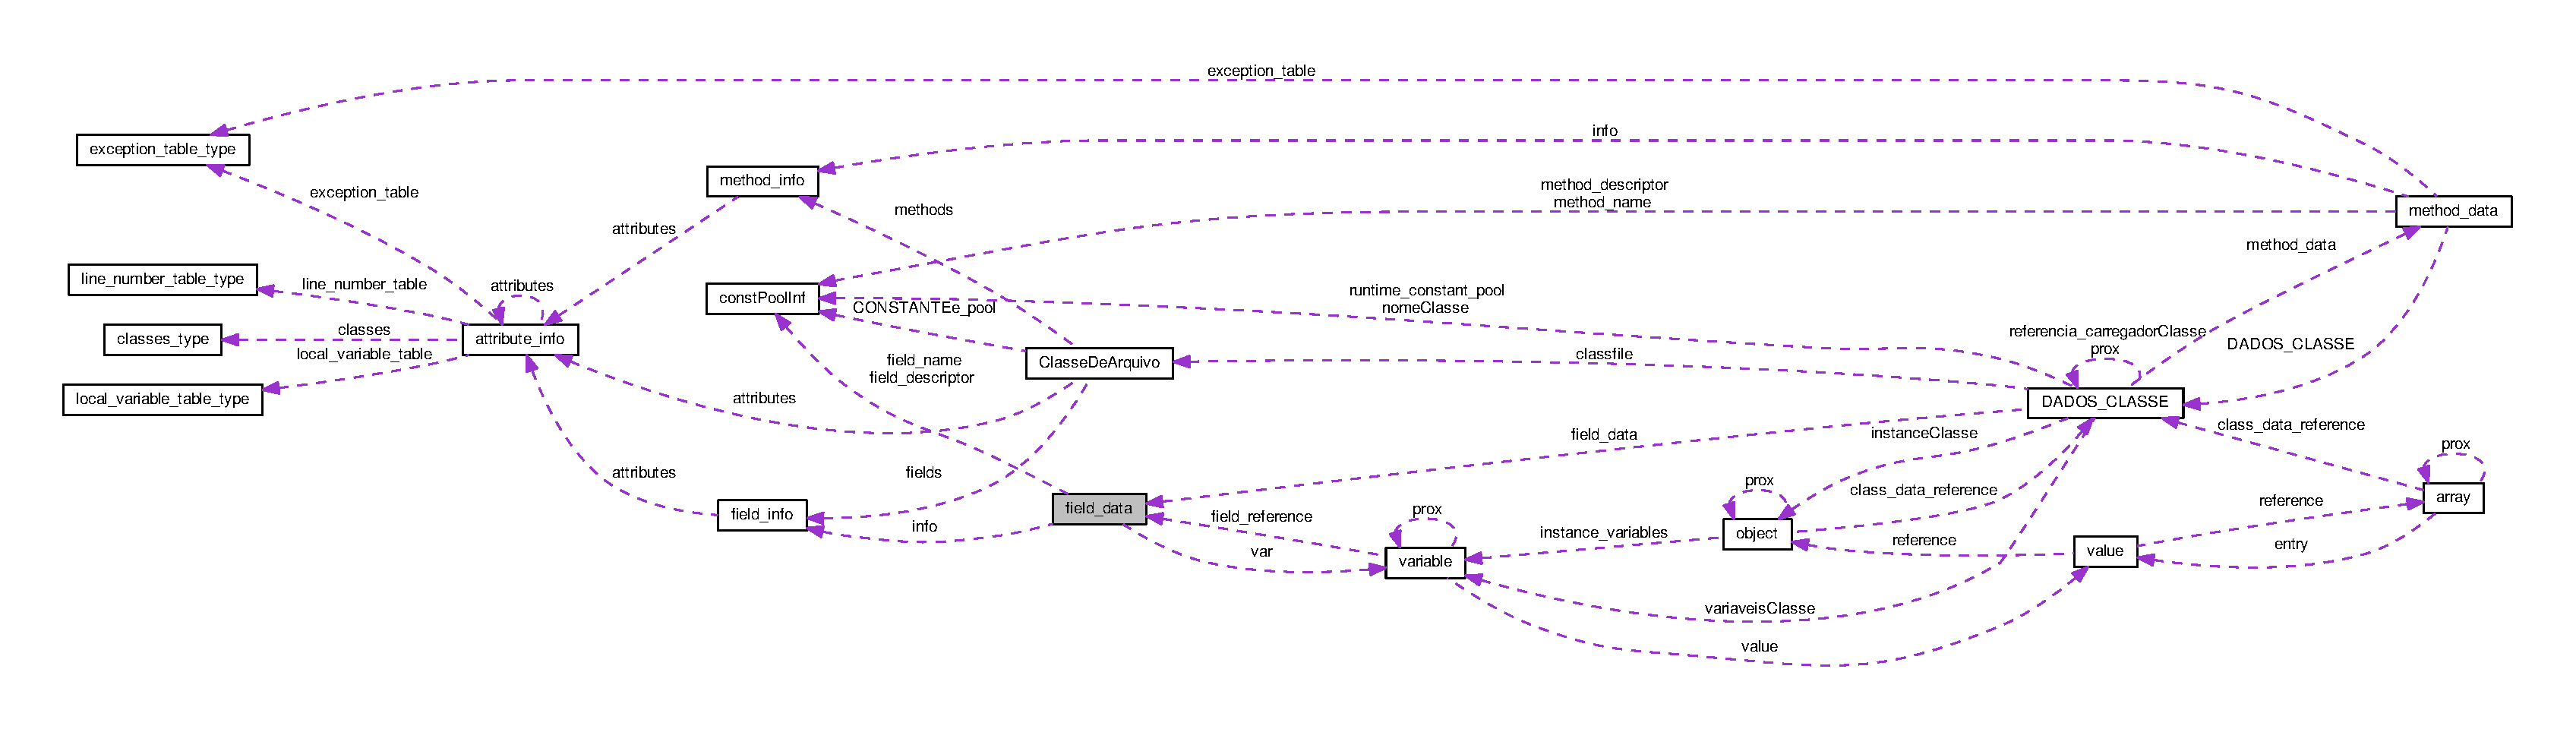
\includegraphics[width=350pt]{structfield__data__coll__graph}
\end{center}
\end{figure}
\subsection*{Atributos Públicos}
\begin{DoxyCompactItemize}
\item 
\hyperlink{structconst_pool_inf}{const\-Pool\-Inf} $\ast$ \hyperlink{structfield__data_a54a2dc5570404dfd1130871d48e2a044}{field\-\_\-name}
\item 
\hyperlink{structconst_pool_inf}{const\-Pool\-Inf} $\ast$ \hyperlink{structfield__data_a4611e29ce2251d6402952826983d17a1}{field\-\_\-descriptor}
\item 
\hyperlink{core_8h_a96376f31c362e2a289072478449290f8}{T\-Y\-P\-E} \hyperlink{structfield__data_a5cf199a1fe02916e0b0e4d27b8d3646f}{field\-\_\-type}
\item 
uint16\-\_\-t \hyperlink{structfield__data_a5d98375dcb4b589355eaf0c96a15eb12}{modifiers}
\item 
\hyperlink{structfield__info}{field\-\_\-info} $\ast$ \hyperlink{structfield__data_a216ebce6db98d903a6b50554a40459a9}{info}
\item 
struct \hyperlink{structvariable}{variable} $\ast$ \hyperlink{structfield__data_a6eb4ec12db5dba2140fff01c6d0439f8}{var}
\end{DoxyCompactItemize}


\subsection{Descrição detalhada}


Definido na linha 123 do ficheiro core.\-h.



\subsection{Documentação dos dados membro}
\hypertarget{structfield__data_a4611e29ce2251d6402952826983d17a1}{\index{field\-\_\-data@{field\-\_\-data}!field\-\_\-descriptor@{field\-\_\-descriptor}}
\index{field\-\_\-descriptor@{field\-\_\-descriptor}!field_data@{field\-\_\-data}}
\subsubsection[{field\-\_\-descriptor}]{\setlength{\rightskip}{0pt plus 5cm}{\bf const\-Pool\-Inf}$\ast$ field\-\_\-data\-::field\-\_\-descriptor}}\label{structfield__data_a4611e29ce2251d6402952826983d17a1}


Definido na linha 125 do ficheiro core.\-h.

\hypertarget{structfield__data_a54a2dc5570404dfd1130871d48e2a044}{\index{field\-\_\-data@{field\-\_\-data}!field\-\_\-name@{field\-\_\-name}}
\index{field\-\_\-name@{field\-\_\-name}!field_data@{field\-\_\-data}}
\subsubsection[{field\-\_\-name}]{\setlength{\rightskip}{0pt plus 5cm}{\bf const\-Pool\-Inf}$\ast$ field\-\_\-data\-::field\-\_\-name}}\label{structfield__data_a54a2dc5570404dfd1130871d48e2a044}


Definido na linha 124 do ficheiro core.\-h.

\hypertarget{structfield__data_a5cf199a1fe02916e0b0e4d27b8d3646f}{\index{field\-\_\-data@{field\-\_\-data}!field\-\_\-type@{field\-\_\-type}}
\index{field\-\_\-type@{field\-\_\-type}!field_data@{field\-\_\-data}}
\subsubsection[{field\-\_\-type}]{\setlength{\rightskip}{0pt plus 5cm}{\bf T\-Y\-P\-E} field\-\_\-data\-::field\-\_\-type}}\label{structfield__data_a5cf199a1fe02916e0b0e4d27b8d3646f}


Definido na linha 126 do ficheiro core.\-h.

\hypertarget{structfield__data_a216ebce6db98d903a6b50554a40459a9}{\index{field\-\_\-data@{field\-\_\-data}!info@{info}}
\index{info@{info}!field_data@{field\-\_\-data}}
\subsubsection[{info}]{\setlength{\rightskip}{0pt plus 5cm}{\bf field\-\_\-info}$\ast$ field\-\_\-data\-::info}}\label{structfield__data_a216ebce6db98d903a6b50554a40459a9}


Definido na linha 128 do ficheiro core.\-h.

\hypertarget{structfield__data_a5d98375dcb4b589355eaf0c96a15eb12}{\index{field\-\_\-data@{field\-\_\-data}!modifiers@{modifiers}}
\index{modifiers@{modifiers}!field_data@{field\-\_\-data}}
\subsubsection[{modifiers}]{\setlength{\rightskip}{0pt plus 5cm}uint16\-\_\-t field\-\_\-data\-::modifiers}}\label{structfield__data_a5d98375dcb4b589355eaf0c96a15eb12}


Definido na linha 127 do ficheiro core.\-h.

\hypertarget{structfield__data_a6eb4ec12db5dba2140fff01c6d0439f8}{\index{field\-\_\-data@{field\-\_\-data}!var@{var}}
\index{var@{var}!field_data@{field\-\_\-data}}
\subsubsection[{var}]{\setlength{\rightskip}{0pt plus 5cm}struct {\bf variable}$\ast$ field\-\_\-data\-::var}}\label{structfield__data_a6eb4ec12db5dba2140fff01c6d0439f8}


Definido na linha 129 do ficheiro core.\-h.



A documentação para esta estrutura foi gerada a partir do seguinte ficheiro\-:\begin{DoxyCompactItemize}
\item 
\hyperlink{core_8h}{core.\-h}\end{DoxyCompactItemize}

\hypertarget{structfield__info}{\section{Referência à estrutura field\-\_\-info}
\label{structfield__info}\index{field\-\_\-info@{field\-\_\-info}}
}


{\ttfamily \#include $<$Leit\-Exib.\-h$>$}



Diagrama de colaboração para field\-\_\-info\-:\nopagebreak
\begin{figure}[H]
\begin{center}
\leavevmode
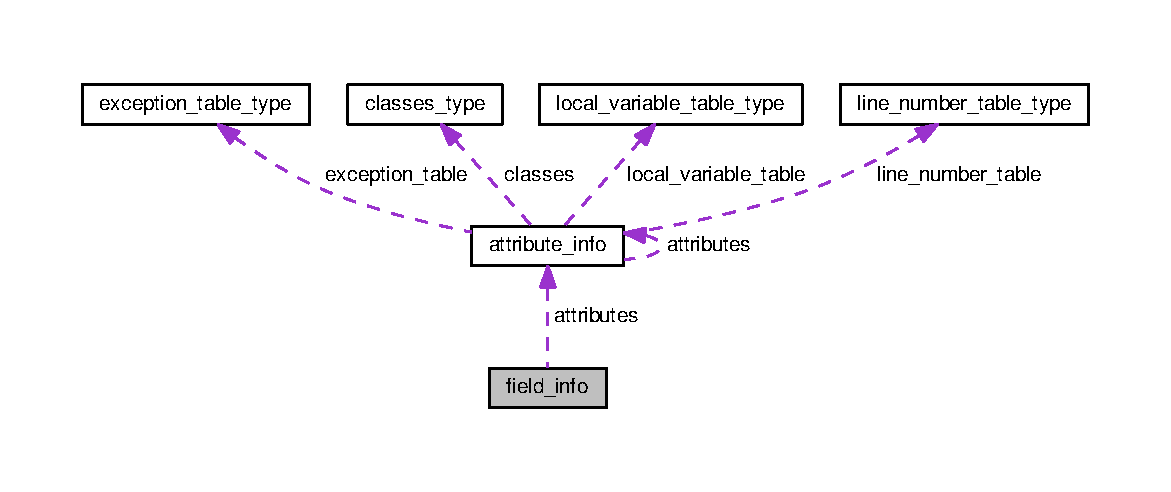
\includegraphics[width=350pt]{structfield__info__coll__graph}
\end{center}
\end{figure}
\subsection*{Atributos Públicos}
\begin{DoxyCompactItemize}
\item 
uint16\-\_\-t \hyperlink{structfield__info_af4858fc71c02c24357fb6be046516331}{flags\-\_\-acesso}
\item 
uint16\-\_\-t \hyperlink{structfield__info_a15c229849e95ecf75de50a79a3760c00}{indicador\-\_\-nome}
\item 
uint16\-\_\-t \hyperlink{structfield__info_a56345eae0135047540b60ca34c91eb46}{descriptor\-\_\-index}
\item 
uint16\-\_\-t \hyperlink{structfield__info_a8da20a3727e18a7f1a7e59cedacaa80c}{conts\-\_\-atributos}
\item 
\hyperlink{structattribute__info}{attribute\-\_\-info} $\ast$ \hyperlink{structfield__info_afdda114944ae5eaae78c237f99257108}{attributes}
\end{DoxyCompactItemize}


\subsection{Descrição detalhada}


Definido na linha 217 do ficheiro Leit\-Exib.\-h.



\subsection{Documentação dos dados membro}
\hypertarget{structfield__info_afdda114944ae5eaae78c237f99257108}{\index{field\-\_\-info@{field\-\_\-info}!attributes@{attributes}}
\index{attributes@{attributes}!field_info@{field\-\_\-info}}
\subsubsection[{attributes}]{\setlength{\rightskip}{0pt plus 5cm}{\bf attribute\-\_\-info}$\ast$ field\-\_\-info\-::attributes}}\label{structfield__info_afdda114944ae5eaae78c237f99257108}


Definido na linha 226 do ficheiro Leit\-Exib.\-h.

\hypertarget{structfield__info_a8da20a3727e18a7f1a7e59cedacaa80c}{\index{field\-\_\-info@{field\-\_\-info}!conts\-\_\-atributos@{conts\-\_\-atributos}}
\index{conts\-\_\-atributos@{conts\-\_\-atributos}!field_info@{field\-\_\-info}}
\subsubsection[{conts\-\_\-atributos}]{\setlength{\rightskip}{0pt plus 5cm}uint16\-\_\-t field\-\_\-info\-::conts\-\_\-atributos}}\label{structfield__info_a8da20a3727e18a7f1a7e59cedacaa80c}


Definido na linha 225 do ficheiro Leit\-Exib.\-h.

\hypertarget{structfield__info_a56345eae0135047540b60ca34c91eb46}{\index{field\-\_\-info@{field\-\_\-info}!descriptor\-\_\-index@{descriptor\-\_\-index}}
\index{descriptor\-\_\-index@{descriptor\-\_\-index}!field_info@{field\-\_\-info}}
\subsubsection[{descriptor\-\_\-index}]{\setlength{\rightskip}{0pt plus 5cm}uint16\-\_\-t field\-\_\-info\-::descriptor\-\_\-index}}\label{structfield__info_a56345eae0135047540b60ca34c91eb46}


Definido na linha 223 do ficheiro Leit\-Exib.\-h.

\hypertarget{structfield__info_af4858fc71c02c24357fb6be046516331}{\index{field\-\_\-info@{field\-\_\-info}!flags\-\_\-acesso@{flags\-\_\-acesso}}
\index{flags\-\_\-acesso@{flags\-\_\-acesso}!field_info@{field\-\_\-info}}
\subsubsection[{flags\-\_\-acesso}]{\setlength{\rightskip}{0pt plus 5cm}uint16\-\_\-t field\-\_\-info\-::flags\-\_\-acesso}}\label{structfield__info_af4858fc71c02c24357fb6be046516331}


Definido na linha 218 do ficheiro Leit\-Exib.\-h.

\hypertarget{structfield__info_a15c229849e95ecf75de50a79a3760c00}{\index{field\-\_\-info@{field\-\_\-info}!indicador\-\_\-nome@{indicador\-\_\-nome}}
\index{indicador\-\_\-nome@{indicador\-\_\-nome}!field_info@{field\-\_\-info}}
\subsubsection[{indicador\-\_\-nome}]{\setlength{\rightskip}{0pt plus 5cm}uint16\-\_\-t field\-\_\-info\-::indicador\-\_\-nome}}\label{structfield__info_a15c229849e95ecf75de50a79a3760c00}


Definido na linha 221 do ficheiro Leit\-Exib.\-h.



A documentação para esta estrutura foi gerada a partir do seguinte ficheiro\-:\begin{DoxyCompactItemize}
\item 
\hyperlink{_leit_exib_8h}{Leit\-Exib.\-h}\end{DoxyCompactItemize}

\hypertarget{structframe}{\section{Referência à estrutura frame}
\label{structframe}\index{frame@{frame}}
}


{\ttfamily \#include $<$core.\-h$>$}



Diagrama de colaboração para frame\-:\nopagebreak
\begin{figure}[H]
\begin{center}
\leavevmode
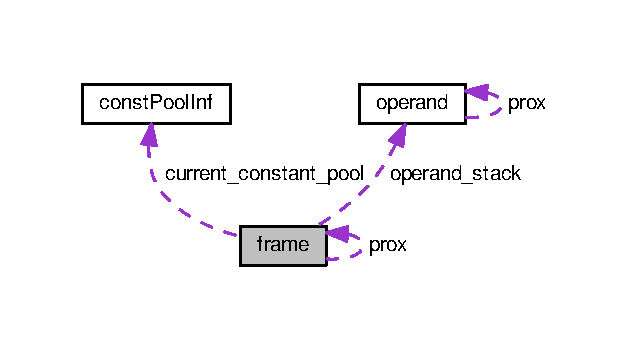
\includegraphics[width=303pt]{structframe__coll__graph}
\end{center}
\end{figure}
\subsection*{Atributos Públicos}
\begin{DoxyCompactItemize}
\item 
uint32\-\_\-t $\ast$ \hyperlink{structframe_afb48efe21a0642a382ef875628272cfd}{local\-\_\-variables}
\item 
\hyperlink{core_8h_a57370c151bf2eefc3bd6e2d13b70e7c9}{O\-P\-E\-R\-A\-N\-D} $\ast$ \hyperlink{structframe_a0e69123161d7ee38be16d922f09dc320}{operand\-\_\-stack}
\item 
\hyperlink{structconst_pool_inf}{const\-Pool\-Inf} $\ast$ \hyperlink{structframe_a44e706fb58a455a533afd748c097c9d0}{current\-\_\-constant\-\_\-pool}
\item 
struct \hyperlink{structframe}{frame} $\ast$ \hyperlink{structframe_ad5c645b97d4a17c7352bf29e7396cea4}{prox}
\end{DoxyCompactItemize}


\subsection{Descrição detalhada}


Definido na linha 98 do ficheiro core.\-h.



\subsection{Documentação dos dados membro}
\hypertarget{structframe_a44e706fb58a455a533afd748c097c9d0}{\index{frame@{frame}!current\-\_\-constant\-\_\-pool@{current\-\_\-constant\-\_\-pool}}
\index{current\-\_\-constant\-\_\-pool@{current\-\_\-constant\-\_\-pool}!frame@{frame}}
\subsubsection[{current\-\_\-constant\-\_\-pool}]{\setlength{\rightskip}{0pt plus 5cm}{\bf const\-Pool\-Inf}$\ast$ frame\-::current\-\_\-constant\-\_\-pool}}\label{structframe_a44e706fb58a455a533afd748c097c9d0}


Definido na linha 101 do ficheiro core.\-h.

\hypertarget{structframe_afb48efe21a0642a382ef875628272cfd}{\index{frame@{frame}!local\-\_\-variables@{local\-\_\-variables}}
\index{local\-\_\-variables@{local\-\_\-variables}!frame@{frame}}
\subsubsection[{local\-\_\-variables}]{\setlength{\rightskip}{0pt plus 5cm}uint32\-\_\-t$\ast$ frame\-::local\-\_\-variables}}\label{structframe_afb48efe21a0642a382ef875628272cfd}


Definido na linha 99 do ficheiro core.\-h.

\hypertarget{structframe_a0e69123161d7ee38be16d922f09dc320}{\index{frame@{frame}!operand\-\_\-stack@{operand\-\_\-stack}}
\index{operand\-\_\-stack@{operand\-\_\-stack}!frame@{frame}}
\subsubsection[{operand\-\_\-stack}]{\setlength{\rightskip}{0pt plus 5cm}{\bf O\-P\-E\-R\-A\-N\-D}$\ast$ frame\-::operand\-\_\-stack}}\label{structframe_a0e69123161d7ee38be16d922f09dc320}


Definido na linha 100 do ficheiro core.\-h.

\hypertarget{structframe_ad5c645b97d4a17c7352bf29e7396cea4}{\index{frame@{frame}!prox@{prox}}
\index{prox@{prox}!frame@{frame}}
\subsubsection[{prox}]{\setlength{\rightskip}{0pt plus 5cm}struct {\bf frame}$\ast$ frame\-::prox}}\label{structframe_ad5c645b97d4a17c7352bf29e7396cea4}


Definido na linha 102 do ficheiro core.\-h.



A documentação para esta estrutura foi gerada a partir do seguinte ficheiro\-:\begin{DoxyCompactItemize}
\item 
\hyperlink{core_8h}{core.\-h}\end{DoxyCompactItemize}

\hypertarget{structheap__area}{\section{Referência à estrutura heap\-\_\-area}
\label{structheap__area}\index{heap\-\_\-area@{heap\-\_\-area}}
}


{\ttfamily \#include $<$core.\-h$>$}



Diagrama de colaboração para heap\-\_\-area\-:\nopagebreak
\begin{figure}[H]
\begin{center}
\leavevmode
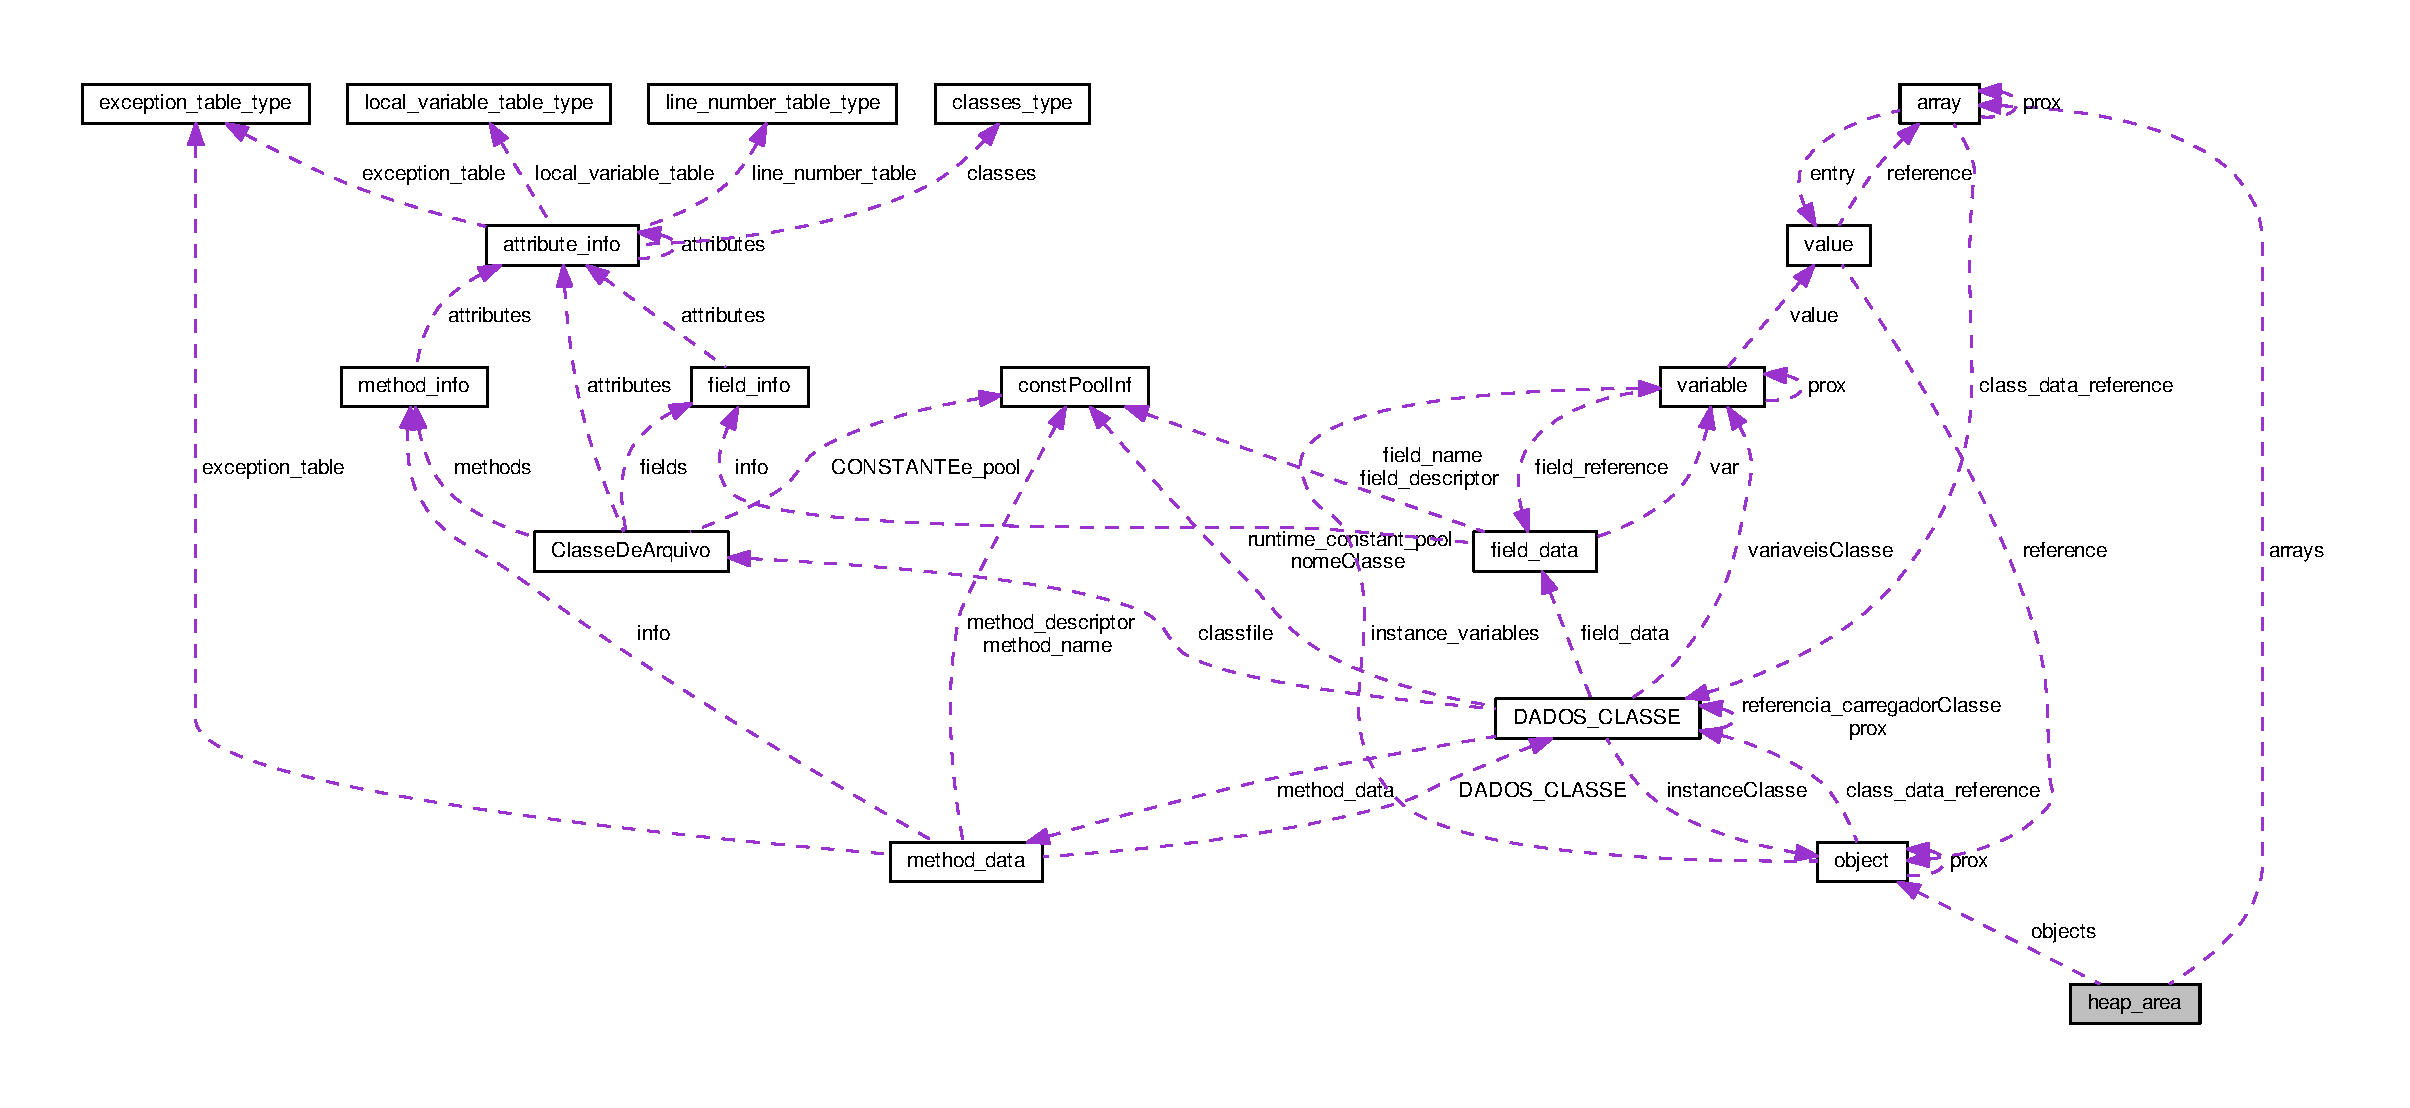
\includegraphics[width=350pt]{structheap__area__coll__graph}
\end{center}
\end{figure}
\subsection*{Atributos Públicos}
\begin{DoxyCompactItemize}
\item 
struct \hyperlink{structobject}{object} $\ast$ \hyperlink{structheap__area_a65ca4dc228035e942540602c47146d29}{objects}
\item 
struct \hyperlink{structarray}{array} $\ast$ \hyperlink{structheap__area_ad0a53fda1a9ad727ee47d6d9a6d155ca}{arrays}
\end{DoxyCompactItemize}


\subsection{Descrição detalhada}


Definido na linha 117 do ficheiro core.\-h.



\subsection{Documentação dos dados membro}
\hypertarget{structheap__area_ad0a53fda1a9ad727ee47d6d9a6d155ca}{\index{heap\-\_\-area@{heap\-\_\-area}!arrays@{arrays}}
\index{arrays@{arrays}!heap_area@{heap\-\_\-area}}
\subsubsection[{arrays}]{\setlength{\rightskip}{0pt plus 5cm}struct {\bf array}$\ast$ heap\-\_\-area\-::arrays}}\label{structheap__area_ad0a53fda1a9ad727ee47d6d9a6d155ca}


Definido na linha 119 do ficheiro core.\-h.

\hypertarget{structheap__area_a65ca4dc228035e942540602c47146d29}{\index{heap\-\_\-area@{heap\-\_\-area}!objects@{objects}}
\index{objects@{objects}!heap_area@{heap\-\_\-area}}
\subsubsection[{objects}]{\setlength{\rightskip}{0pt plus 5cm}struct {\bf object}$\ast$ heap\-\_\-area\-::objects}}\label{structheap__area_a65ca4dc228035e942540602c47146d29}


Definido na linha 118 do ficheiro core.\-h.



A documentação para esta estrutura foi gerada a partir do seguinte ficheiro\-:\begin{DoxyCompactItemize}
\item 
\hyperlink{core_8h}{core.\-h}\end{DoxyCompactItemize}

\hypertarget{structjvm}{\section{Referência à estrutura jvm}
\label{structjvm}\index{jvm@{jvm}}
}


{\ttfamily \#include $<$core.\-h$>$}



Diagrama de colaboração para jvm\-:\nopagebreak
\begin{figure}[H]
\begin{center}
\leavevmode
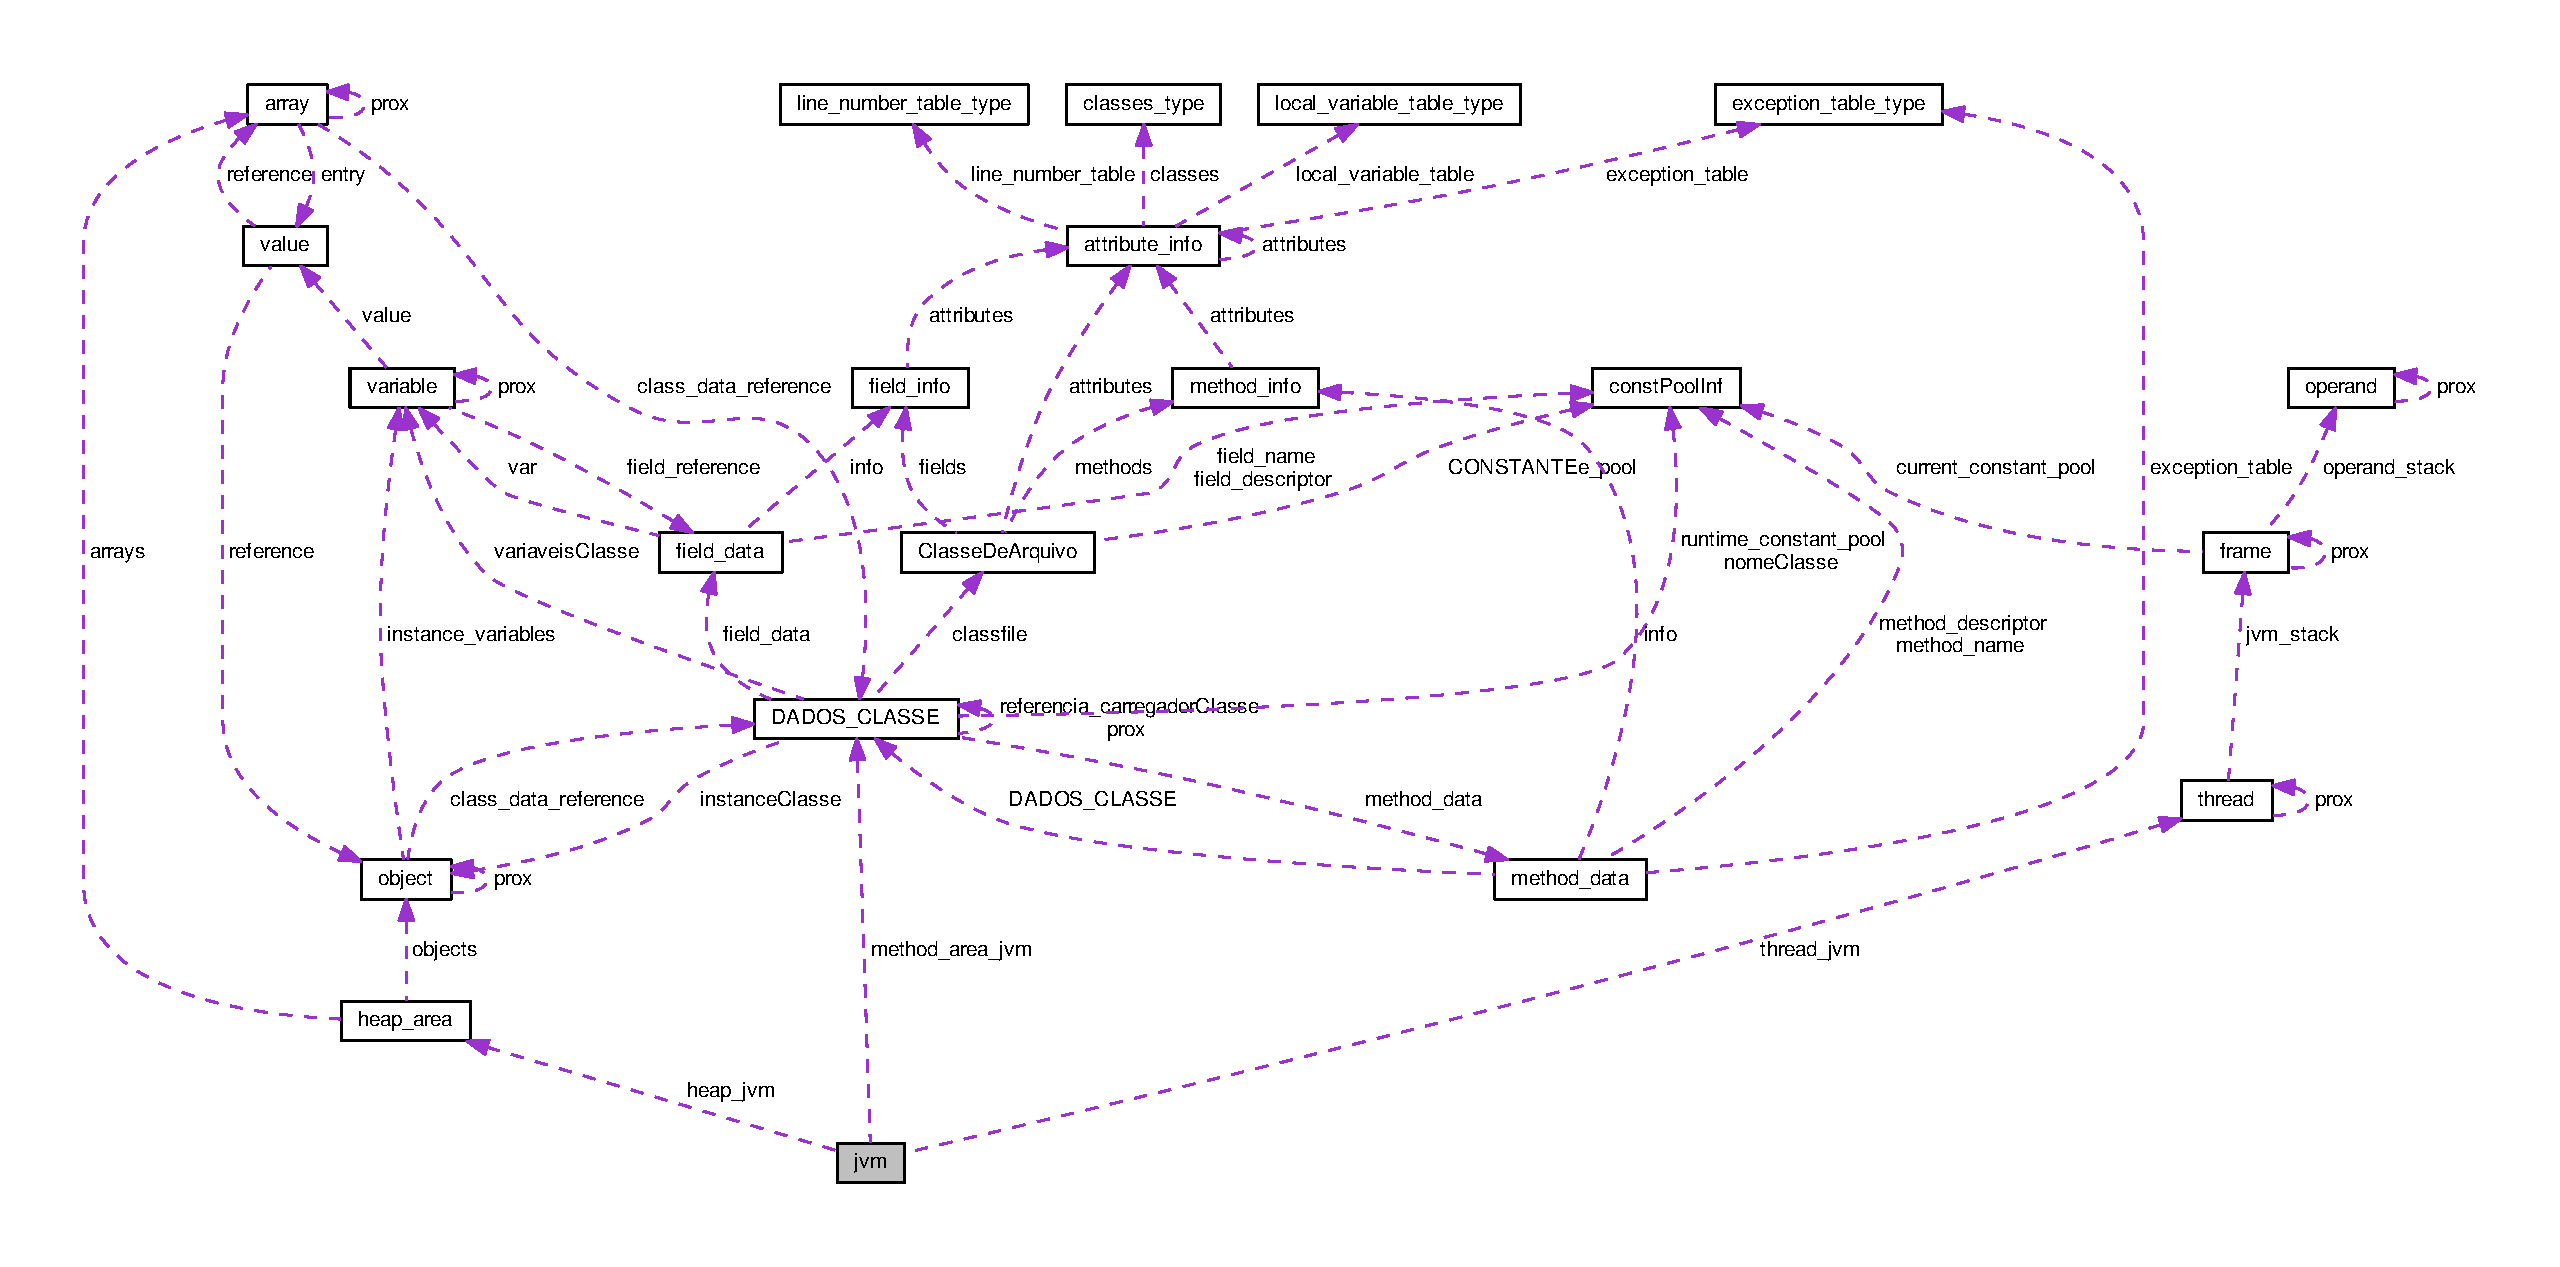
\includegraphics[width=350pt]{structjvm__coll__graph}
\end{center}
\end{figure}
\subsection*{Atributos Públicos}
\begin{DoxyCompactItemize}
\item 
\hyperlink{core_8h_ad43b7ffe97b146f9dce917ae2a0fd181}{T\-H\-R\-E\-A\-D} $\ast$ \hyperlink{structjvm_a95875933adbaab4bef10b00738ba0722}{thread\-\_\-jvm}
\item 
\hyperlink{core_8h_a8aa4d8af3cc19c82a17fa714d533cb8f}{H\-E\-A\-P\-\_\-\-A\-R\-E\-A} $\ast$ \hyperlink{structjvm_aaa2c1b91d2f8feef91b7e1e8552a873f}{heap\-\_\-jvm}
\item 
\hyperlink{struct_d_a_d_o_s___c_l_a_s_s_e}{D\-A\-D\-O\-S\-\_\-\-C\-L\-A\-S\-S\-E} $\ast$ \hyperlink{structjvm_ac8c89a213f0d332aff40faa2661b97e3}{method\-\_\-area\-\_\-jvm}
\end{DoxyCompactItemize}


\subsection{Descrição detalhada}


Definido na linha 185 do ficheiro core.\-h.



\subsection{Documentação dos dados membro}
\hypertarget{structjvm_aaa2c1b91d2f8feef91b7e1e8552a873f}{\index{jvm@{jvm}!heap\-\_\-jvm@{heap\-\_\-jvm}}
\index{heap\-\_\-jvm@{heap\-\_\-jvm}!jvm@{jvm}}
\subsubsection[{heap\-\_\-jvm}]{\setlength{\rightskip}{0pt plus 5cm}{\bf H\-E\-A\-P\-\_\-\-A\-R\-E\-A}$\ast$ jvm\-::heap\-\_\-jvm}}\label{structjvm_aaa2c1b91d2f8feef91b7e1e8552a873f}


Definido na linha 187 do ficheiro core.\-h.

\hypertarget{structjvm_ac8c89a213f0d332aff40faa2661b97e3}{\index{jvm@{jvm}!method\-\_\-area\-\_\-jvm@{method\-\_\-area\-\_\-jvm}}
\index{method\-\_\-area\-\_\-jvm@{method\-\_\-area\-\_\-jvm}!jvm@{jvm}}
\subsubsection[{method\-\_\-area\-\_\-jvm}]{\setlength{\rightskip}{0pt plus 5cm}{\bf D\-A\-D\-O\-S\-\_\-\-C\-L\-A\-S\-S\-E}$\ast$ jvm\-::method\-\_\-area\-\_\-jvm}}\label{structjvm_ac8c89a213f0d332aff40faa2661b97e3}


Definido na linha 189 do ficheiro core.\-h.

\hypertarget{structjvm_a95875933adbaab4bef10b00738ba0722}{\index{jvm@{jvm}!thread\-\_\-jvm@{thread\-\_\-jvm}}
\index{thread\-\_\-jvm@{thread\-\_\-jvm}!jvm@{jvm}}
\subsubsection[{thread\-\_\-jvm}]{\setlength{\rightskip}{0pt plus 5cm}{\bf T\-H\-R\-E\-A\-D}$\ast$ jvm\-::thread\-\_\-jvm}}\label{structjvm_a95875933adbaab4bef10b00738ba0722}


Definido na linha 186 do ficheiro core.\-h.



A documentação para esta estrutura foi gerada a partir do seguinte ficheiro\-:\begin{DoxyCompactItemize}
\item 
\hyperlink{core_8h}{core.\-h}\end{DoxyCompactItemize}

\hypertarget{structline__number__table__type}{\section{Referência à estrutura line\-\_\-number\-\_\-table\-\_\-type}
\label{structline__number__table__type}\index{line\-\_\-number\-\_\-table\-\_\-type@{line\-\_\-number\-\_\-table\-\_\-type}}
}


{\ttfamily \#include $<$Leit\-Exib.\-h$>$}

\subsection*{Atributos Públicos}
\begin{DoxyCompactItemize}
\item 
uint16\-\_\-t \hyperlink{structline__number__table__type_a5b5fc96901fd52be22ddc5115633ed3c}{start\-\_\-pc}
\item 
uint16\-\_\-t \hyperlink{structline__number__table__type_a85fe37c92e96597234cdfdad035f1ae4}{line\-\_\-number}
\end{DoxyCompactItemize}


\subsection{Descrição detalhada}


Definido na linha 150 do ficheiro Leit\-Exib.\-h.



\subsection{Documentação dos dados membro}
\hypertarget{structline__number__table__type_a85fe37c92e96597234cdfdad035f1ae4}{\index{line\-\_\-number\-\_\-table\-\_\-type@{line\-\_\-number\-\_\-table\-\_\-type}!line\-\_\-number@{line\-\_\-number}}
\index{line\-\_\-number@{line\-\_\-number}!line_number_table_type@{line\-\_\-number\-\_\-table\-\_\-type}}
\subsubsection[{line\-\_\-number}]{\setlength{\rightskip}{0pt plus 5cm}uint16\-\_\-t line\-\_\-number\-\_\-table\-\_\-type\-::line\-\_\-number}}\label{structline__number__table__type_a85fe37c92e96597234cdfdad035f1ae4}


Definido na linha 152 do ficheiro Leit\-Exib.\-h.

\hypertarget{structline__number__table__type_a5b5fc96901fd52be22ddc5115633ed3c}{\index{line\-\_\-number\-\_\-table\-\_\-type@{line\-\_\-number\-\_\-table\-\_\-type}!start\-\_\-pc@{start\-\_\-pc}}
\index{start\-\_\-pc@{start\-\_\-pc}!line_number_table_type@{line\-\_\-number\-\_\-table\-\_\-type}}
\subsubsection[{start\-\_\-pc}]{\setlength{\rightskip}{0pt plus 5cm}uint16\-\_\-t line\-\_\-number\-\_\-table\-\_\-type\-::start\-\_\-pc}}\label{structline__number__table__type_a5b5fc96901fd52be22ddc5115633ed3c}


Definido na linha 151 do ficheiro Leit\-Exib.\-h.



A documentação para esta estrutura foi gerada a partir do seguinte ficheiro\-:\begin{DoxyCompactItemize}
\item 
\hyperlink{_leit_exib_8h}{Leit\-Exib.\-h}\end{DoxyCompactItemize}

\hypertarget{structlocal__variable__table__type}{\section{Referência à estrutura local\-\_\-variable\-\_\-table\-\_\-type}
\label{structlocal__variable__table__type}\index{local\-\_\-variable\-\_\-table\-\_\-type@{local\-\_\-variable\-\_\-table\-\_\-type}}
}


{\ttfamily \#include $<$Leit\-Exib.\-h$>$}

\subsection*{Atributos Públicos}
\begin{DoxyCompactItemize}
\item 
uint16\-\_\-t \hyperlink{structlocal__variable__table__type_a560d45b628c0adaf0f1716b001d49379}{start\-\_\-pc}
\item 
uint16\-\_\-t \hyperlink{structlocal__variable__table__type_a0dc62ed5079cc1226d9c254287009198}{length}
\item 
uint16\-\_\-t \hyperlink{structlocal__variable__table__type_a2e30d42da683da1dfc3a45e07dde62ec}{indicador\-\_\-nome}
\item 
uint16\-\_\-t \hyperlink{structlocal__variable__table__type_a3c1df7fc91bfab07bce2ab1e19084fe8}{descriptor\-\_\-index}
\item 
uint16\-\_\-t \hyperlink{structlocal__variable__table__type_a99e8d85f07bd570440689f229e4e0fa1}{index}
\end{DoxyCompactItemize}


\subsection{Descrição detalhada}


Definido na linha 155 do ficheiro Leit\-Exib.\-h.



\subsection{Documentação dos dados membro}
\hypertarget{structlocal__variable__table__type_a3c1df7fc91bfab07bce2ab1e19084fe8}{\index{local\-\_\-variable\-\_\-table\-\_\-type@{local\-\_\-variable\-\_\-table\-\_\-type}!descriptor\-\_\-index@{descriptor\-\_\-index}}
\index{descriptor\-\_\-index@{descriptor\-\_\-index}!local_variable_table_type@{local\-\_\-variable\-\_\-table\-\_\-type}}
\subsubsection[{descriptor\-\_\-index}]{\setlength{\rightskip}{0pt plus 5cm}uint16\-\_\-t local\-\_\-variable\-\_\-table\-\_\-type\-::descriptor\-\_\-index}}\label{structlocal__variable__table__type_a3c1df7fc91bfab07bce2ab1e19084fe8}


Definido na linha 159 do ficheiro Leit\-Exib.\-h.

\hypertarget{structlocal__variable__table__type_a99e8d85f07bd570440689f229e4e0fa1}{\index{local\-\_\-variable\-\_\-table\-\_\-type@{local\-\_\-variable\-\_\-table\-\_\-type}!index@{index}}
\index{index@{index}!local_variable_table_type@{local\-\_\-variable\-\_\-table\-\_\-type}}
\subsubsection[{index}]{\setlength{\rightskip}{0pt plus 5cm}uint16\-\_\-t local\-\_\-variable\-\_\-table\-\_\-type\-::index}}\label{structlocal__variable__table__type_a99e8d85f07bd570440689f229e4e0fa1}


Definido na linha 160 do ficheiro Leit\-Exib.\-h.

\hypertarget{structlocal__variable__table__type_a2e30d42da683da1dfc3a45e07dde62ec}{\index{local\-\_\-variable\-\_\-table\-\_\-type@{local\-\_\-variable\-\_\-table\-\_\-type}!indicador\-\_\-nome@{indicador\-\_\-nome}}
\index{indicador\-\_\-nome@{indicador\-\_\-nome}!local_variable_table_type@{local\-\_\-variable\-\_\-table\-\_\-type}}
\subsubsection[{indicador\-\_\-nome}]{\setlength{\rightskip}{0pt plus 5cm}uint16\-\_\-t local\-\_\-variable\-\_\-table\-\_\-type\-::indicador\-\_\-nome}}\label{structlocal__variable__table__type_a2e30d42da683da1dfc3a45e07dde62ec}


Definido na linha 158 do ficheiro Leit\-Exib.\-h.

\hypertarget{structlocal__variable__table__type_a0dc62ed5079cc1226d9c254287009198}{\index{local\-\_\-variable\-\_\-table\-\_\-type@{local\-\_\-variable\-\_\-table\-\_\-type}!length@{length}}
\index{length@{length}!local_variable_table_type@{local\-\_\-variable\-\_\-table\-\_\-type}}
\subsubsection[{length}]{\setlength{\rightskip}{0pt plus 5cm}uint16\-\_\-t local\-\_\-variable\-\_\-table\-\_\-type\-::length}}\label{structlocal__variable__table__type_a0dc62ed5079cc1226d9c254287009198}


Definido na linha 157 do ficheiro Leit\-Exib.\-h.

\hypertarget{structlocal__variable__table__type_a560d45b628c0adaf0f1716b001d49379}{\index{local\-\_\-variable\-\_\-table\-\_\-type@{local\-\_\-variable\-\_\-table\-\_\-type}!start\-\_\-pc@{start\-\_\-pc}}
\index{start\-\_\-pc@{start\-\_\-pc}!local_variable_table_type@{local\-\_\-variable\-\_\-table\-\_\-type}}
\subsubsection[{start\-\_\-pc}]{\setlength{\rightskip}{0pt plus 5cm}uint16\-\_\-t local\-\_\-variable\-\_\-table\-\_\-type\-::start\-\_\-pc}}\label{structlocal__variable__table__type_a560d45b628c0adaf0f1716b001d49379}


Definido na linha 156 do ficheiro Leit\-Exib.\-h.



A documentação para esta estrutura foi gerada a partir do seguinte ficheiro\-:\begin{DoxyCompactItemize}
\item 
\hyperlink{_leit_exib_8h}{Leit\-Exib.\-h}\end{DoxyCompactItemize}

\hypertarget{structmethod__data}{\section{Referência à estrutura method\-\_\-data}
\label{structmethod__data}\index{method\-\_\-data@{method\-\_\-data}}
}


{\ttfamily \#include $<$core.\-h$>$}



Diagrama de colaboração para method\-\_\-data\-:\nopagebreak
\begin{figure}[H]
\begin{center}
\leavevmode
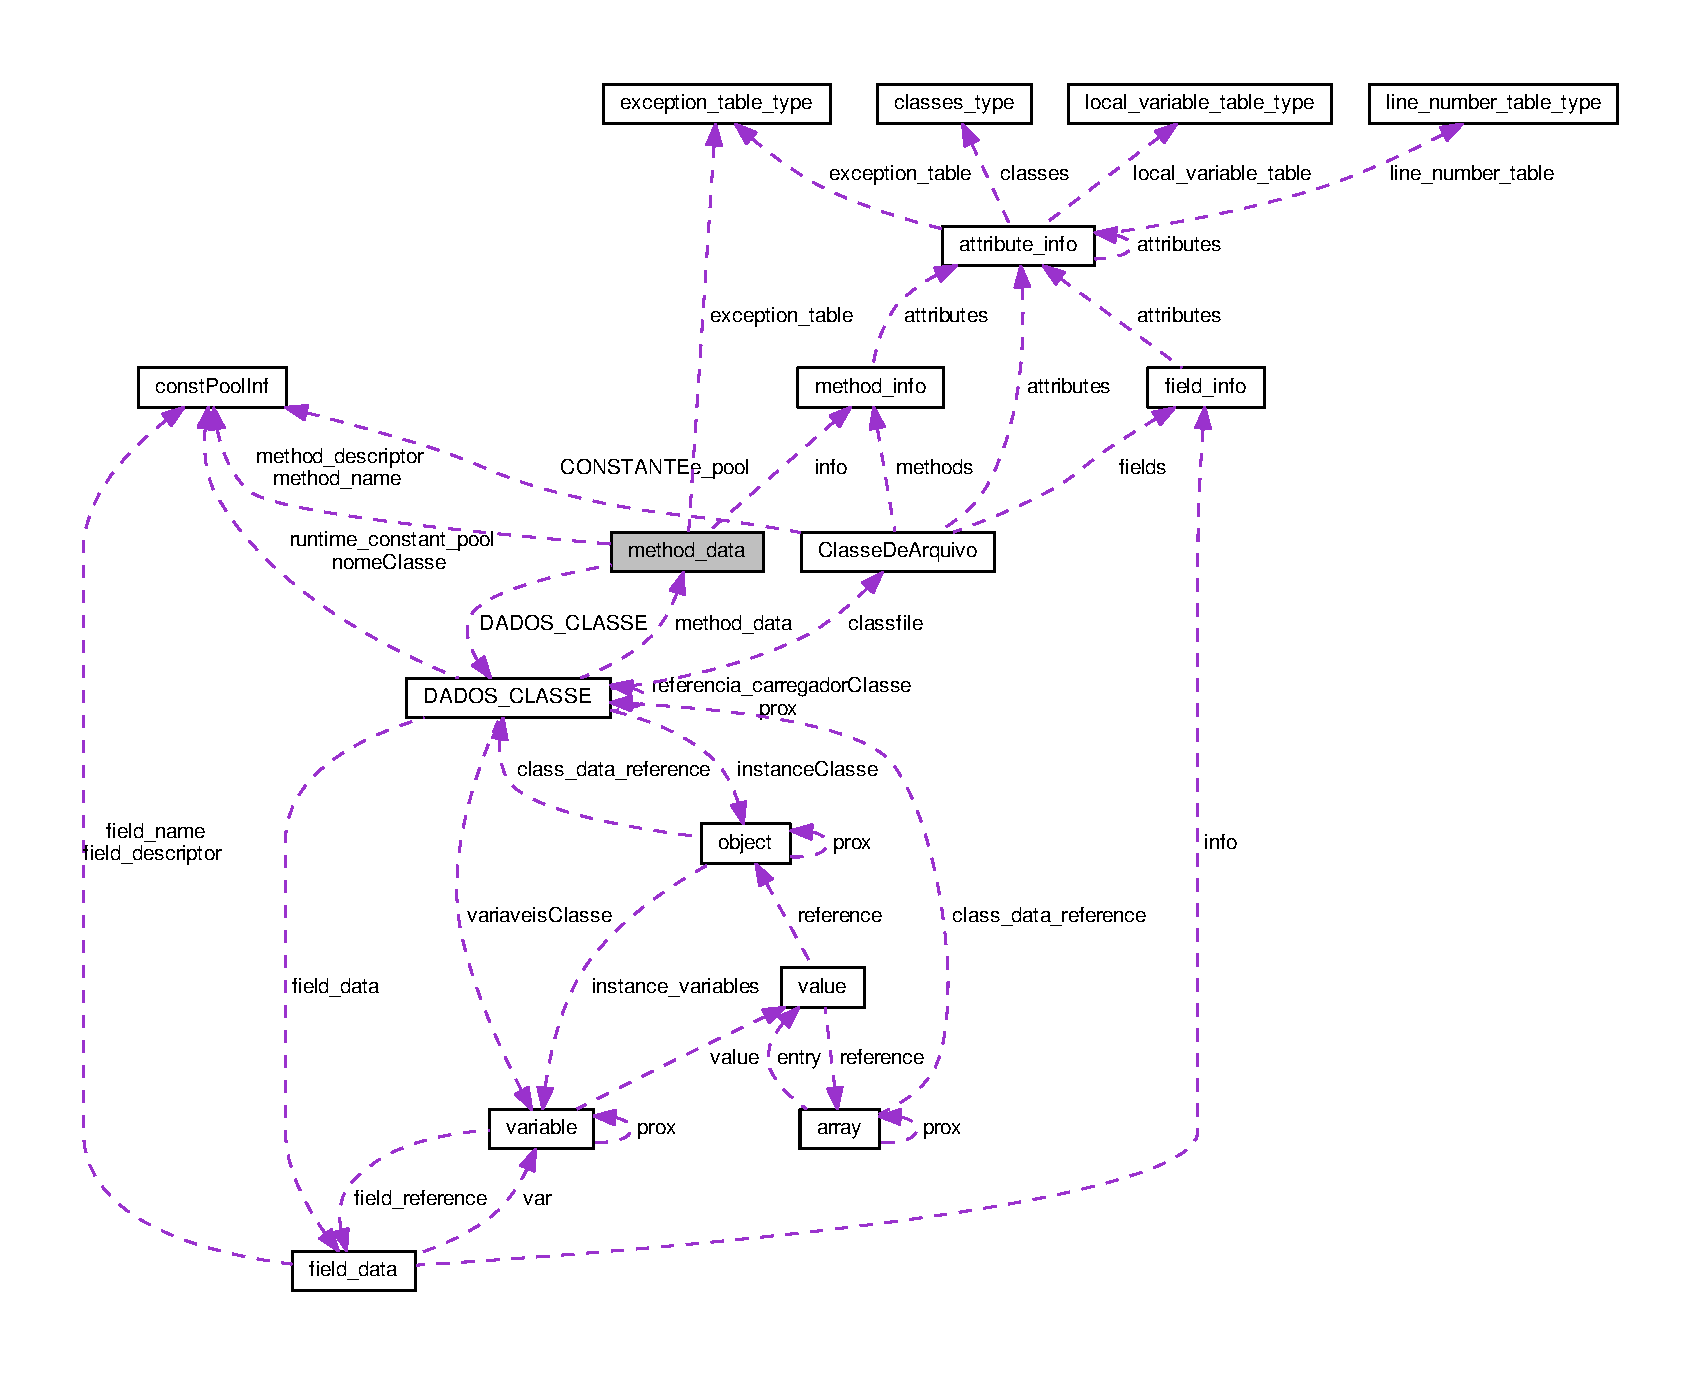
\includegraphics[width=350pt]{structmethod__data__coll__graph}
\end{center}
\end{figure}
\subsection*{Atributos Públicos}
\begin{DoxyCompactItemize}
\item 
\hyperlink{structconst_pool_inf}{const\-Pool\-Inf} $\ast$ \hyperlink{structmethod__data_acc4747daee0a91ee73f94422c8b833ab}{method\-\_\-name}
\item 
\hyperlink{structconst_pool_inf}{const\-Pool\-Inf} $\ast$ \hyperlink{structmethod__data_ae4a01197c105855d2e337fb8875358a8}{method\-\_\-descriptor}
\item 
uint16\-\_\-t \hyperlink{structmethod__data_a2abb22d9f683ff1163f58d9b071902bd}{modifiers}
\item 
struct \hyperlink{struct_d_a_d_o_s___c_l_a_s_s_e}{D\-A\-D\-O\-S\-\_\-\-C\-L\-A\-S\-S\-E} $\ast$ \hyperlink{structmethod__data_a2a372a889aabaea0e0b4a08be11cbfa3}{D\-A\-D\-O\-S\-\_\-\-C\-L\-A\-S\-S\-E}
\item 
uint32\-\_\-t \hyperlink{structmethod__data_a9c6035e8b389eea9bc15f380cffefe8b}{code\-\_\-length}
\item 
uint8\-\_\-t $\ast$ \hyperlink{structmethod__data_a602f386ab76983d72ba48488f8c309a9}{bytecodes}
\item 
uint16\-\_\-t \hyperlink{structmethod__data_a0c23eae5e5fe3302c9c1b7f8e5543e3c}{stack\-\_\-size}
\item 
uint16\-\_\-t \hyperlink{structmethod__data_a09b30df4053904e1ebe666ae1ccc45d4}{locals\-\_\-size}
\item 
uint16\-\_\-t \hyperlink{structmethod__data_ac5f08aab5ad351365c25e550c4a0bfb3}{exception\-\_\-table\-\_\-length}
\item 
\hyperlink{structexception__table__type}{exception\-\_\-table\-\_\-type} $\ast$ \hyperlink{structmethod__data_ad9179cc8edbe4688c2f97359cc05ccd0}{exception\-\_\-table}
\item 
\hyperlink{structmethod__info}{method\-\_\-info} $\ast$ \hyperlink{structmethod__data_ae433725619fdadbb915ae3f51198208b}{info}
\end{DoxyCompactItemize}


\subsection{Descrição detalhada}


Definido na linha 141 do ficheiro core.\-h.



\subsection{Documentação dos dados membro}
\hypertarget{structmethod__data_a602f386ab76983d72ba48488f8c309a9}{\index{method\-\_\-data@{method\-\_\-data}!bytecodes@{bytecodes}}
\index{bytecodes@{bytecodes}!method_data@{method\-\_\-data}}
\subsubsection[{bytecodes}]{\setlength{\rightskip}{0pt plus 5cm}uint8\-\_\-t$\ast$ method\-\_\-data\-::bytecodes}}\label{structmethod__data_a602f386ab76983d72ba48488f8c309a9}


Definido na linha 148 do ficheiro core.\-h.

\hypertarget{structmethod__data_a9c6035e8b389eea9bc15f380cffefe8b}{\index{method\-\_\-data@{method\-\_\-data}!code\-\_\-length@{code\-\_\-length}}
\index{code\-\_\-length@{code\-\_\-length}!method_data@{method\-\_\-data}}
\subsubsection[{code\-\_\-length}]{\setlength{\rightskip}{0pt plus 5cm}uint32\-\_\-t method\-\_\-data\-::code\-\_\-length}}\label{structmethod__data_a9c6035e8b389eea9bc15f380cffefe8b}


Definido na linha 147 do ficheiro core.\-h.

\hypertarget{structmethod__data_a2a372a889aabaea0e0b4a08be11cbfa3}{\index{method\-\_\-data@{method\-\_\-data}!D\-A\-D\-O\-S\-\_\-\-C\-L\-A\-S\-S\-E@{D\-A\-D\-O\-S\-\_\-\-C\-L\-A\-S\-S\-E}}
\index{D\-A\-D\-O\-S\-\_\-\-C\-L\-A\-S\-S\-E@{D\-A\-D\-O\-S\-\_\-\-C\-L\-A\-S\-S\-E}!method_data@{method\-\_\-data}}
\subsubsection[{D\-A\-D\-O\-S\-\_\-\-C\-L\-A\-S\-S\-E}]{\setlength{\rightskip}{0pt plus 5cm}struct {\bf D\-A\-D\-O\-S\-\_\-\-C\-L\-A\-S\-S\-E}$\ast$ method\-\_\-data\-::\-D\-A\-D\-O\-S\-\_\-\-C\-L\-A\-S\-S\-E}}\label{structmethod__data_a2a372a889aabaea0e0b4a08be11cbfa3}


Definido na linha 145 do ficheiro core.\-h.

\hypertarget{structmethod__data_ad9179cc8edbe4688c2f97359cc05ccd0}{\index{method\-\_\-data@{method\-\_\-data}!exception\-\_\-table@{exception\-\_\-table}}
\index{exception\-\_\-table@{exception\-\_\-table}!method_data@{method\-\_\-data}}
\subsubsection[{exception\-\_\-table}]{\setlength{\rightskip}{0pt plus 5cm}{\bf exception\-\_\-table\-\_\-type}$\ast$ method\-\_\-data\-::exception\-\_\-table}}\label{structmethod__data_ad9179cc8edbe4688c2f97359cc05ccd0}


Definido na linha 152 do ficheiro core.\-h.

\hypertarget{structmethod__data_ac5f08aab5ad351365c25e550c4a0bfb3}{\index{method\-\_\-data@{method\-\_\-data}!exception\-\_\-table\-\_\-length@{exception\-\_\-table\-\_\-length}}
\index{exception\-\_\-table\-\_\-length@{exception\-\_\-table\-\_\-length}!method_data@{method\-\_\-data}}
\subsubsection[{exception\-\_\-table\-\_\-length}]{\setlength{\rightskip}{0pt plus 5cm}uint16\-\_\-t method\-\_\-data\-::exception\-\_\-table\-\_\-length}}\label{structmethod__data_ac5f08aab5ad351365c25e550c4a0bfb3}


Definido na linha 151 do ficheiro core.\-h.

\hypertarget{structmethod__data_ae433725619fdadbb915ae3f51198208b}{\index{method\-\_\-data@{method\-\_\-data}!info@{info}}
\index{info@{info}!method_data@{method\-\_\-data}}
\subsubsection[{info}]{\setlength{\rightskip}{0pt plus 5cm}{\bf method\-\_\-info}$\ast$ method\-\_\-data\-::info}}\label{structmethod__data_ae433725619fdadbb915ae3f51198208b}


Definido na linha 153 do ficheiro core.\-h.

\hypertarget{structmethod__data_a09b30df4053904e1ebe666ae1ccc45d4}{\index{method\-\_\-data@{method\-\_\-data}!locals\-\_\-size@{locals\-\_\-size}}
\index{locals\-\_\-size@{locals\-\_\-size}!method_data@{method\-\_\-data}}
\subsubsection[{locals\-\_\-size}]{\setlength{\rightskip}{0pt plus 5cm}uint16\-\_\-t method\-\_\-data\-::locals\-\_\-size}}\label{structmethod__data_a09b30df4053904e1ebe666ae1ccc45d4}


Definido na linha 150 do ficheiro core.\-h.

\hypertarget{structmethod__data_ae4a01197c105855d2e337fb8875358a8}{\index{method\-\_\-data@{method\-\_\-data}!method\-\_\-descriptor@{method\-\_\-descriptor}}
\index{method\-\_\-descriptor@{method\-\_\-descriptor}!method_data@{method\-\_\-data}}
\subsubsection[{method\-\_\-descriptor}]{\setlength{\rightskip}{0pt plus 5cm}{\bf const\-Pool\-Inf}$\ast$ method\-\_\-data\-::method\-\_\-descriptor}}\label{structmethod__data_ae4a01197c105855d2e337fb8875358a8}


Definido na linha 143 do ficheiro core.\-h.

\hypertarget{structmethod__data_acc4747daee0a91ee73f94422c8b833ab}{\index{method\-\_\-data@{method\-\_\-data}!method\-\_\-name@{method\-\_\-name}}
\index{method\-\_\-name@{method\-\_\-name}!method_data@{method\-\_\-data}}
\subsubsection[{method\-\_\-name}]{\setlength{\rightskip}{0pt plus 5cm}{\bf const\-Pool\-Inf}$\ast$ method\-\_\-data\-::method\-\_\-name}}\label{structmethod__data_acc4747daee0a91ee73f94422c8b833ab}


Definido na linha 142 do ficheiro core.\-h.

\hypertarget{structmethod__data_a2abb22d9f683ff1163f58d9b071902bd}{\index{method\-\_\-data@{method\-\_\-data}!modifiers@{modifiers}}
\index{modifiers@{modifiers}!method_data@{method\-\_\-data}}
\subsubsection[{modifiers}]{\setlength{\rightskip}{0pt plus 5cm}uint16\-\_\-t method\-\_\-data\-::modifiers}}\label{structmethod__data_a2abb22d9f683ff1163f58d9b071902bd}


Definido na linha 144 do ficheiro core.\-h.

\hypertarget{structmethod__data_a0c23eae5e5fe3302c9c1b7f8e5543e3c}{\index{method\-\_\-data@{method\-\_\-data}!stack\-\_\-size@{stack\-\_\-size}}
\index{stack\-\_\-size@{stack\-\_\-size}!method_data@{method\-\_\-data}}
\subsubsection[{stack\-\_\-size}]{\setlength{\rightskip}{0pt plus 5cm}uint16\-\_\-t method\-\_\-data\-::stack\-\_\-size}}\label{structmethod__data_a0c23eae5e5fe3302c9c1b7f8e5543e3c}


Definido na linha 149 do ficheiro core.\-h.



A documentação para esta estrutura foi gerada a partir do seguinte ficheiro\-:\begin{DoxyCompactItemize}
\item 
\hyperlink{core_8h}{core.\-h}\end{DoxyCompactItemize}

\hypertarget{structmethod__info}{\section{Referência à estrutura method\-\_\-info}
\label{structmethod__info}\index{method\-\_\-info@{method\-\_\-info}}
}


{\ttfamily \#include $<$Leit\-Exib.\-h$>$}



Diagrama de colaboração para method\-\_\-info\-:\nopagebreak
\begin{figure}[H]
\begin{center}
\leavevmode
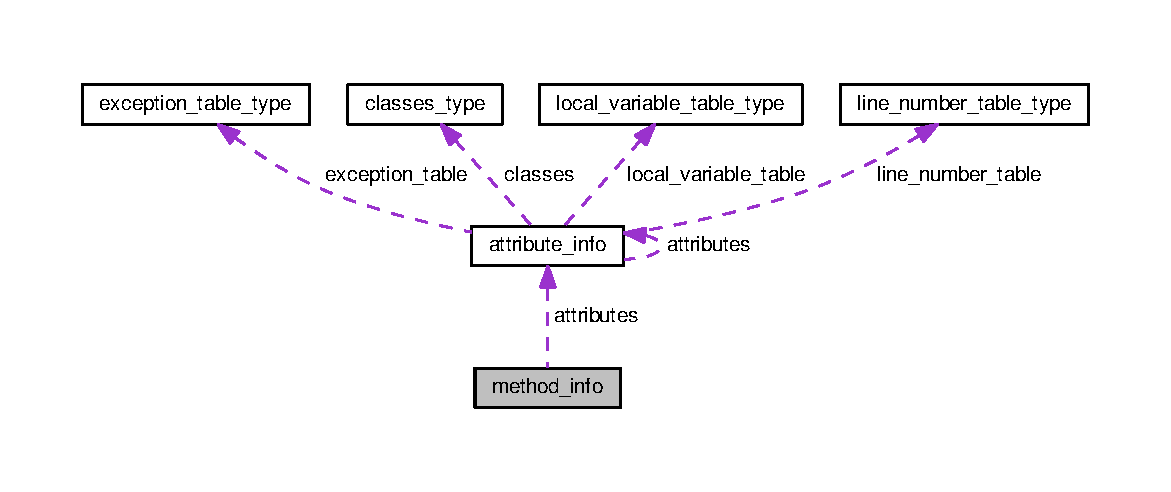
\includegraphics[width=350pt]{structmethod__info__coll__graph}
\end{center}
\end{figure}
\subsection*{Atributos Públicos}
\begin{DoxyCompactItemize}
\item 
uint16\-\_\-t \hyperlink{structmethod__info_a200169cf04858f0fe263f2b905ccb0bf}{flags\-\_\-acesso}
\item 
uint16\-\_\-t \hyperlink{structmethod__info_af759f4abed4c00637446765268f8c4cf}{indicador\-\_\-nome}
\item 
uint16\-\_\-t \hyperlink{structmethod__info_abccd6a5202d4c0ee1be6b89692d0352a}{descriptor\-\_\-index}
\item 
uint16\-\_\-t \hyperlink{structmethod__info_a23e8e7b47fe7f4e69e00b96313ec76ad}{conts\-\_\-atributos}
\item 
\hyperlink{structattribute__info}{attribute\-\_\-info} $\ast$ \hyperlink{structmethod__info_a8ce4caaa03680c91f548558a38647ad8}{attributes}
\end{DoxyCompactItemize}


\subsection{Descrição detalhada}


Definido na linha 230 do ficheiro Leit\-Exib.\-h.



\subsection{Documentação dos dados membro}
\hypertarget{structmethod__info_a8ce4caaa03680c91f548558a38647ad8}{\index{method\-\_\-info@{method\-\_\-info}!attributes@{attributes}}
\index{attributes@{attributes}!method_info@{method\-\_\-info}}
\subsubsection[{attributes}]{\setlength{\rightskip}{0pt plus 5cm}{\bf attribute\-\_\-info}$\ast$ method\-\_\-info\-::attributes}}\label{structmethod__info_a8ce4caaa03680c91f548558a38647ad8}


Definido na linha 240 do ficheiro Leit\-Exib.\-h.

\hypertarget{structmethod__info_a23e8e7b47fe7f4e69e00b96313ec76ad}{\index{method\-\_\-info@{method\-\_\-info}!conts\-\_\-atributos@{conts\-\_\-atributos}}
\index{conts\-\_\-atributos@{conts\-\_\-atributos}!method_info@{method\-\_\-info}}
\subsubsection[{conts\-\_\-atributos}]{\setlength{\rightskip}{0pt plus 5cm}uint16\-\_\-t method\-\_\-info\-::conts\-\_\-atributos}}\label{structmethod__info_a23e8e7b47fe7f4e69e00b96313ec76ad}


Definido na linha 239 do ficheiro Leit\-Exib.\-h.

\hypertarget{structmethod__info_abccd6a5202d4c0ee1be6b89692d0352a}{\index{method\-\_\-info@{method\-\_\-info}!descriptor\-\_\-index@{descriptor\-\_\-index}}
\index{descriptor\-\_\-index@{descriptor\-\_\-index}!method_info@{method\-\_\-info}}
\subsubsection[{descriptor\-\_\-index}]{\setlength{\rightskip}{0pt plus 5cm}uint16\-\_\-t method\-\_\-info\-::descriptor\-\_\-index}}\label{structmethod__info_abccd6a5202d4c0ee1be6b89692d0352a}


Definido na linha 237 do ficheiro Leit\-Exib.\-h.

\hypertarget{structmethod__info_a200169cf04858f0fe263f2b905ccb0bf}{\index{method\-\_\-info@{method\-\_\-info}!flags\-\_\-acesso@{flags\-\_\-acesso}}
\index{flags\-\_\-acesso@{flags\-\_\-acesso}!method_info@{method\-\_\-info}}
\subsubsection[{flags\-\_\-acesso}]{\setlength{\rightskip}{0pt plus 5cm}uint16\-\_\-t method\-\_\-info\-::flags\-\_\-acesso}}\label{structmethod__info_a200169cf04858f0fe263f2b905ccb0bf}


Definido na linha 231 do ficheiro Leit\-Exib.\-h.

\hypertarget{structmethod__info_af759f4abed4c00637446765268f8c4cf}{\index{method\-\_\-info@{method\-\_\-info}!indicador\-\_\-nome@{indicador\-\_\-nome}}
\index{indicador\-\_\-nome@{indicador\-\_\-nome}!method_info@{method\-\_\-info}}
\subsubsection[{indicador\-\_\-nome}]{\setlength{\rightskip}{0pt plus 5cm}uint16\-\_\-t method\-\_\-info\-::indicador\-\_\-nome}}\label{structmethod__info_af759f4abed4c00637446765268f8c4cf}


Definido na linha 234 do ficheiro Leit\-Exib.\-h.



A documentação para esta estrutura foi gerada a partir do seguinte ficheiro\-:\begin{DoxyCompactItemize}
\item 
\hyperlink{_leit_exib_8h}{Leit\-Exib.\-h}\end{DoxyCompactItemize}

\hypertarget{structobject}{\section{Referência à estrutura object}
\label{structobject}\index{object@{object}}
}


{\ttfamily \#include $<$core.\-h$>$}



Diagrama de colaboração para object\-:\nopagebreak
\begin{figure}[H]
\begin{center}
\leavevmode
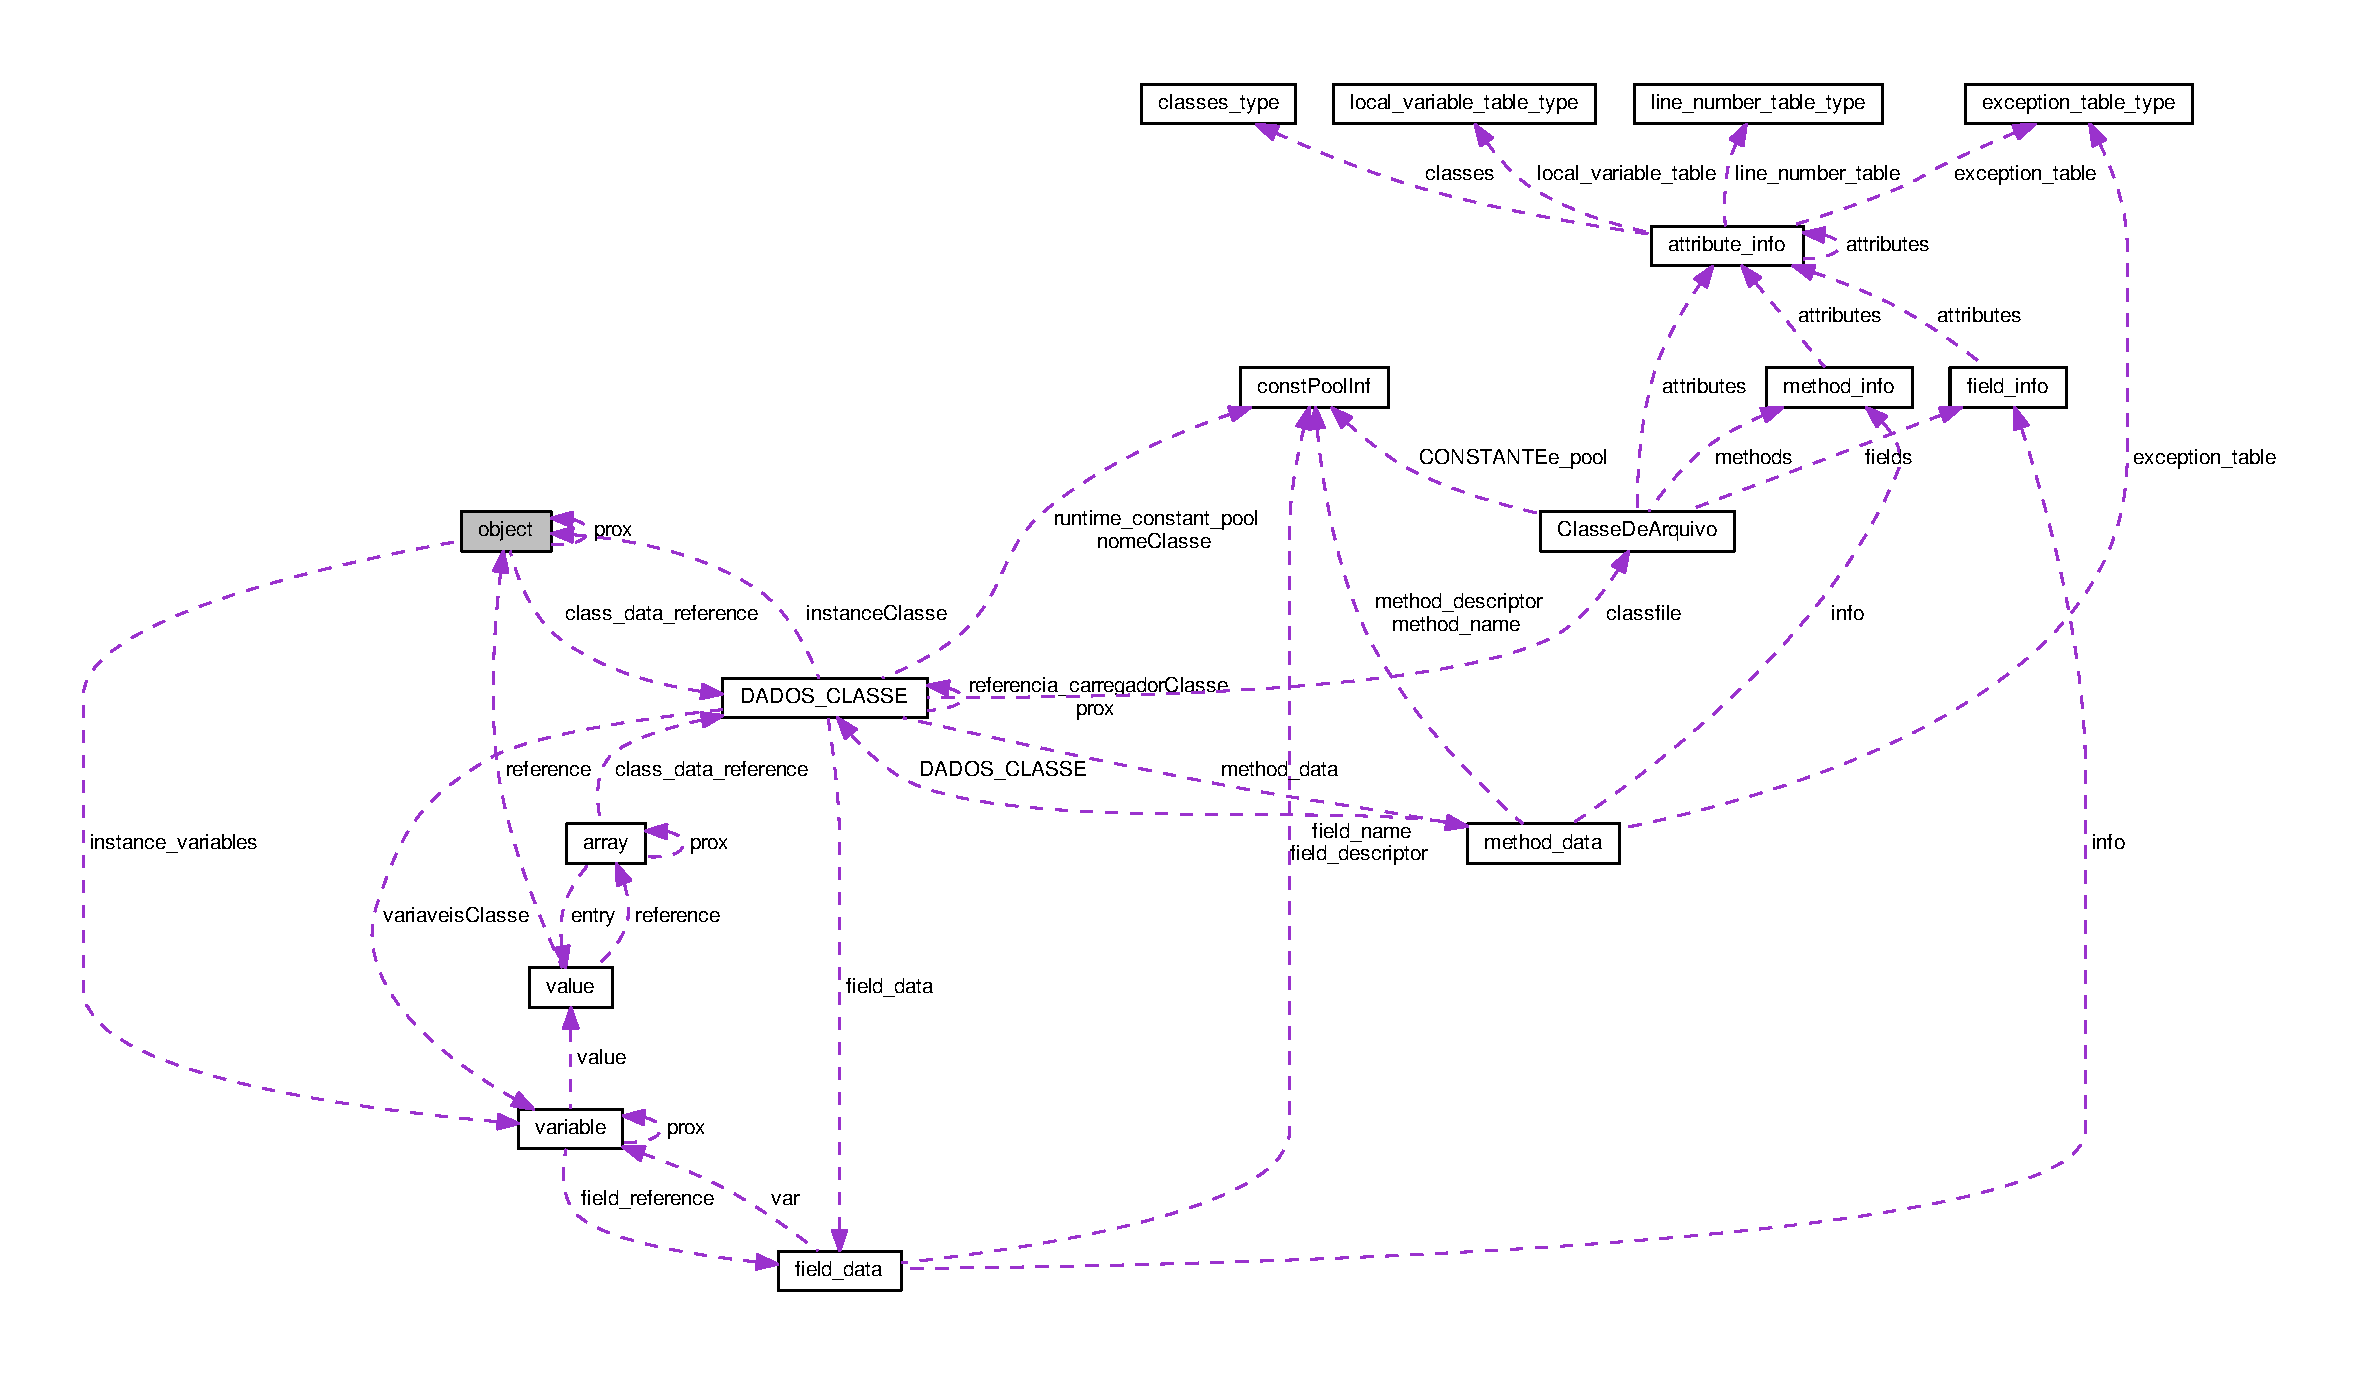
\includegraphics[width=350pt]{structobject__coll__graph}
\end{center}
\end{figure}
\subsection*{Atributos Públicos}
\begin{DoxyCompactItemize}
\item 
\hyperlink{struct_d_a_d_o_s___c_l_a_s_s_e}{D\-A\-D\-O\-S\-\_\-\-C\-L\-A\-S\-S\-E} $\ast$ \hyperlink{structobject_af7136e313255a7d1efdcf775c9f6c412}{class\-\_\-data\-\_\-reference}
\item 
\hyperlink{core_8h_a85b40991452ad00efae1784148c94402}{V\-A\-R\-I\-A\-B\-L\-E} $\ast$ \hyperlink{structobject_ad02cb265ba006796debd79c5e22902d3}{instance\-\_\-variables}
\item 
struct \hyperlink{structobject}{object} $\ast$ \hyperlink{structobject_adc7a300d54dbdc7f5a72f145b30ff3da}{prox}
\end{DoxyCompactItemize}


\subsection{Descrição detalhada}


Definido na linha 170 do ficheiro core.\-h.



\subsection{Documentação dos dados membro}
\hypertarget{structobject_af7136e313255a7d1efdcf775c9f6c412}{\index{object@{object}!class\-\_\-data\-\_\-reference@{class\-\_\-data\-\_\-reference}}
\index{class\-\_\-data\-\_\-reference@{class\-\_\-data\-\_\-reference}!object@{object}}
\subsubsection[{class\-\_\-data\-\_\-reference}]{\setlength{\rightskip}{0pt plus 5cm}{\bf D\-A\-D\-O\-S\-\_\-\-C\-L\-A\-S\-S\-E}$\ast$ object\-::class\-\_\-data\-\_\-reference}}\label{structobject_af7136e313255a7d1efdcf775c9f6c412}


Definido na linha 171 do ficheiro core.\-h.

\hypertarget{structobject_ad02cb265ba006796debd79c5e22902d3}{\index{object@{object}!instance\-\_\-variables@{instance\-\_\-variables}}
\index{instance\-\_\-variables@{instance\-\_\-variables}!object@{object}}
\subsubsection[{instance\-\_\-variables}]{\setlength{\rightskip}{0pt plus 5cm}{\bf V\-A\-R\-I\-A\-B\-L\-E}$\ast$ object\-::instance\-\_\-variables}}\label{structobject_ad02cb265ba006796debd79c5e22902d3}


Definido na linha 172 do ficheiro core.\-h.

\hypertarget{structobject_adc7a300d54dbdc7f5a72f145b30ff3da}{\index{object@{object}!prox@{prox}}
\index{prox@{prox}!object@{object}}
\subsubsection[{prox}]{\setlength{\rightskip}{0pt plus 5cm}struct {\bf object}$\ast$ object\-::prox}}\label{structobject_adc7a300d54dbdc7f5a72f145b30ff3da}


Definido na linha 173 do ficheiro core.\-h.



A documentação para esta estrutura foi gerada a partir do seguinte ficheiro\-:\begin{DoxyCompactItemize}
\item 
\hyperlink{core_8h}{core.\-h}\end{DoxyCompactItemize}

\hypertarget{structoperand}{\section{Referência à estrutura operand}
\label{structoperand}\index{operand@{operand}}
}


{\ttfamily \#include $<$core.\-h$>$}



Diagrama de colaboração para operand\-:\nopagebreak
\begin{figure}[H]
\begin{center}
\leavevmode
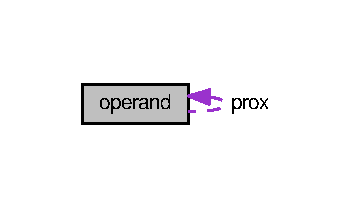
\includegraphics[width=170pt]{structoperand__coll__graph}
\end{center}
\end{figure}
\subsection*{Atributos Públicos}
\begin{DoxyCompactItemize}
\item 
uint32\-\_\-t \hyperlink{structoperand_a4112f16b41c272f45499c809391b17a2}{value}
\item 
\hyperlink{core_8h_a96376f31c362e2a289072478449290f8}{T\-Y\-P\-E} \hyperlink{structoperand_a8af3746223d14253f5b287d236f59ce4}{type}
\item 
struct \hyperlink{structoperand}{operand} $\ast$ \hyperlink{structoperand_a49e5a5dbe02eaa10b1a29b71106f9910}{prox}
\end{DoxyCompactItemize}


\subsection{Descrição detalhada}


Definido na linha 91 do ficheiro core.\-h.



\subsection{Documentação dos dados membro}
\hypertarget{structoperand_a49e5a5dbe02eaa10b1a29b71106f9910}{\index{operand@{operand}!prox@{prox}}
\index{prox@{prox}!operand@{operand}}
\subsubsection[{prox}]{\setlength{\rightskip}{0pt plus 5cm}struct {\bf operand}$\ast$ operand\-::prox}}\label{structoperand_a49e5a5dbe02eaa10b1a29b71106f9910}


Definido na linha 94 do ficheiro core.\-h.

\hypertarget{structoperand_a8af3746223d14253f5b287d236f59ce4}{\index{operand@{operand}!type@{type}}
\index{type@{type}!operand@{operand}}
\subsubsection[{type}]{\setlength{\rightskip}{0pt plus 5cm}{\bf T\-Y\-P\-E} operand\-::type}}\label{structoperand_a8af3746223d14253f5b287d236f59ce4}


Definido na linha 93 do ficheiro core.\-h.

\hypertarget{structoperand_a4112f16b41c272f45499c809391b17a2}{\index{operand@{operand}!value@{value}}
\index{value@{value}!operand@{operand}}
\subsubsection[{value}]{\setlength{\rightskip}{0pt plus 5cm}uint32\-\_\-t operand\-::value}}\label{structoperand_a4112f16b41c272f45499c809391b17a2}


Definido na linha 92 do ficheiro core.\-h.



A documentação para esta estrutura foi gerada a partir do seguinte ficheiro\-:\begin{DoxyCompactItemize}
\item 
\hyperlink{core_8h}{core.\-h}\end{DoxyCompactItemize}

\hypertarget{structthread}{\section{Referência à estrutura thread}
\label{structthread}\index{thread@{thread}}
}


{\ttfamily \#include $<$core.\-h$>$}



Diagrama de colaboração para thread\-:\nopagebreak
\begin{figure}[H]
\begin{center}
\leavevmode
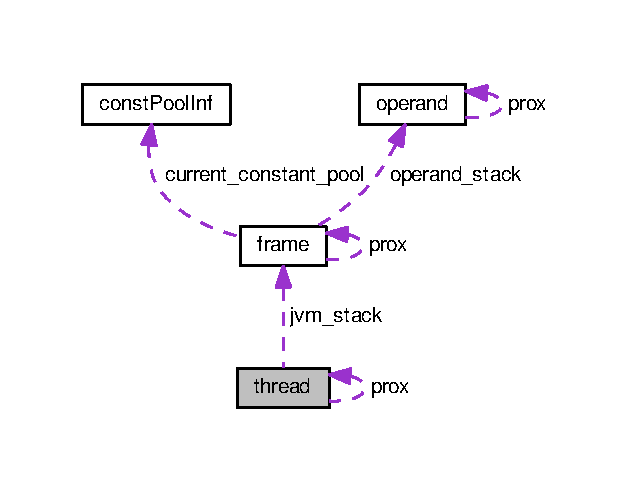
\includegraphics[width=303pt]{structthread__coll__graph}
\end{center}
\end{figure}
\subsection*{Atributos Públicos}
\begin{DoxyCompactItemize}
\item 
\hyperlink{core_8h_ab34056db44556fbb28ffa6aff4873b4c}{O\-P\-C\-O\-D\-E} $\ast$ \hyperlink{structthread_ab5f04be4cab8242e674775d1538dfa43}{program\-\_\-counter}
\item 
\hyperlink{core_8h_ad2c7f62ece09f452ea1a5285adcc503c}{F\-R\-A\-M\-E} $\ast$ \hyperlink{structthread_a45e1dff8e8c5d2981ee351857fbd765c}{jvm\-\_\-stack}
\item 
struct \hyperlink{structthread}{thread} $\ast$ \hyperlink{structthread_aa2c034fdf01f832556b8bf192ab57dcc}{prox}
\end{DoxyCompactItemize}


\subsection{Descrição detalhada}


Definido na linha 107 do ficheiro core.\-h.



\subsection{Documentação dos dados membro}
\hypertarget{structthread_a45e1dff8e8c5d2981ee351857fbd765c}{\index{thread@{thread}!jvm\-\_\-stack@{jvm\-\_\-stack}}
\index{jvm\-\_\-stack@{jvm\-\_\-stack}!thread@{thread}}
\subsubsection[{jvm\-\_\-stack}]{\setlength{\rightskip}{0pt plus 5cm}{\bf F\-R\-A\-M\-E}$\ast$ thread\-::jvm\-\_\-stack}}\label{structthread_a45e1dff8e8c5d2981ee351857fbd765c}


Definido na linha 111 do ficheiro core.\-h.

\hypertarget{structthread_ab5f04be4cab8242e674775d1538dfa43}{\index{thread@{thread}!program\-\_\-counter@{program\-\_\-counter}}
\index{program\-\_\-counter@{program\-\_\-counter}!thread@{thread}}
\subsubsection[{program\-\_\-counter}]{\setlength{\rightskip}{0pt plus 5cm}{\bf O\-P\-C\-O\-D\-E}$\ast$ thread\-::program\-\_\-counter}}\label{structthread_ab5f04be4cab8242e674775d1538dfa43}


Definido na linha 109 do ficheiro core.\-h.

\hypertarget{structthread_aa2c034fdf01f832556b8bf192ab57dcc}{\index{thread@{thread}!prox@{prox}}
\index{prox@{prox}!thread@{thread}}
\subsubsection[{prox}]{\setlength{\rightskip}{0pt plus 5cm}struct {\bf thread}$\ast$ thread\-::prox}}\label{structthread_aa2c034fdf01f832556b8bf192ab57dcc}


Definido na linha 112 do ficheiro core.\-h.



A documentação para esta estrutura foi gerada a partir do seguinte ficheiro\-:\begin{DoxyCompactItemize}
\item 
\hyperlink{core_8h}{core.\-h}\end{DoxyCompactItemize}

\hypertarget{structvalue}{\section{Referência à estrutura value}
\label{structvalue}\index{value@{value}}
}


{\ttfamily \#include $<$core.\-h$>$}



Diagrama de colaboração para value\-:\nopagebreak
\begin{figure}[H]
\begin{center}
\leavevmode
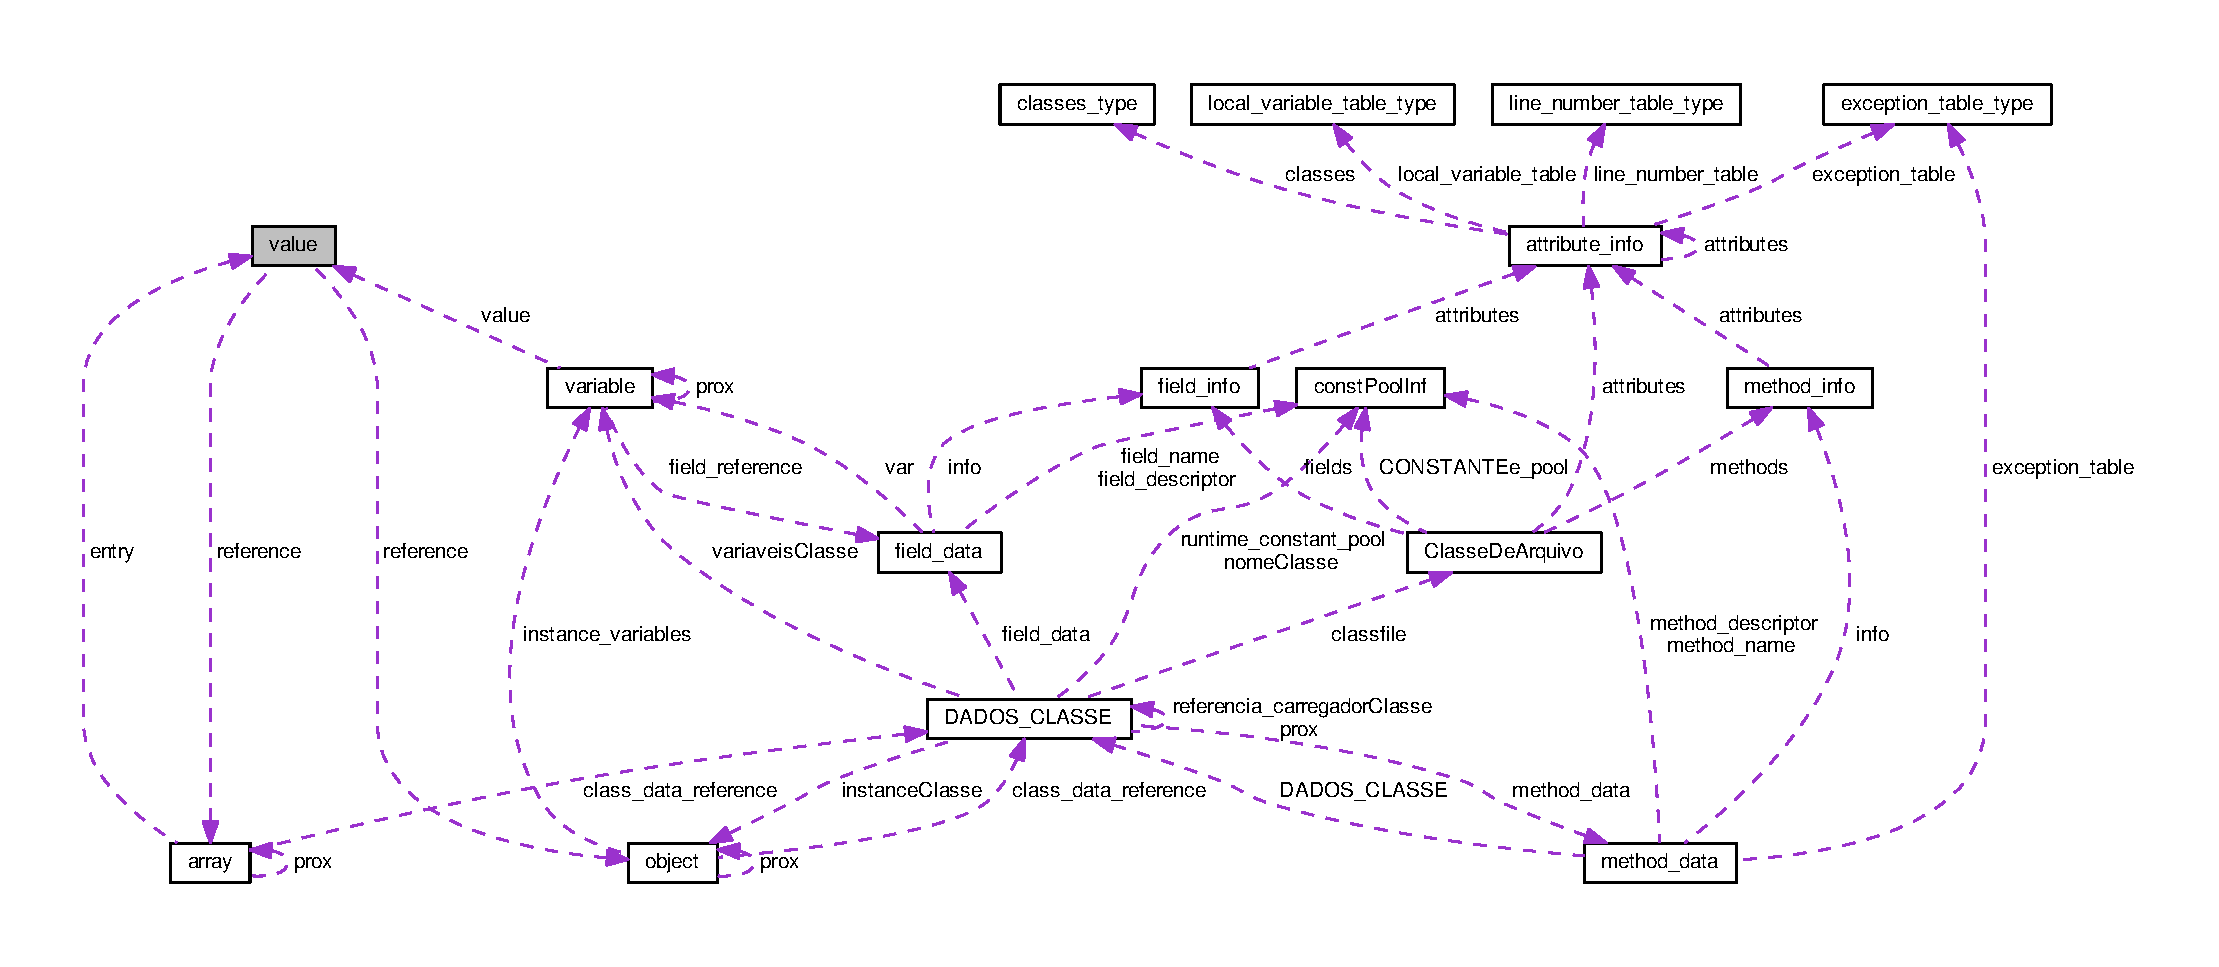
\includegraphics[width=350pt]{structvalue__coll__graph}
\end{center}
\end{figure}
\subsection*{Atributos Públicos}
\begin{DoxyCompactItemize}
\item 
\hyperlink{core_8h_a96376f31c362e2a289072478449290f8}{T\-Y\-P\-E} \hyperlink{structvalue_a8193b2471a420d07d6273ea3c9653155}{type}
\item 
\begin{tabbing}
xx\=xx\=xx\=xx\=xx\=xx\=xx\=xx\=xx\=\kill
union \{\\
\>struct \{\\
\>\>int8\_t \hyperlink{structvalue_a5827febe7b21adba8ddb86bbf0996e8c}{byte}\\
\>\} \hyperlink{structvalue_af2bea3c5b60d0a36c10e297af2bbb80f}{Byte}\\
\>struct \{\\
\>\>int16\_t \hyperlink{structvalue_a083e8a03606d5b79029794b3d575c021}{short\_}\\
\>\} \hyperlink{structvalue_ac6f6c8288a2314221cd061b264fa25e1}{Short}\\
\>struct \{\\
\>\>int32\_t \hyperlink{structvalue_a58a1dfb88538dd68c4ccd5d6c7f571d2}{integer}\\
\>\} \hyperlink{structvalue_a8f62817042c944120cd6099cc5ec9654}{Integer}\\
\>struct \{\\
\>\>uint32\_t \hyperlink{structvalue_a670628f51376fadc6cd3c7aa2076dd95}{high\_bytes}\\
\>\>uint32\_t \hyperlink{structvalue_a8f7d961af70bd80fe990c31ff3db48fa}{low\_bytes}\\
\>\} \hyperlink{structvalue_a525db6e48cfe9e5303f30ba1dde3cb7f}{Long}\\
\>struct \{\\
\>\>uint32\_t \hyperlink{structvalue_af597140f73eb1550b593c1b98557f6b8}{float\_}\\
\>\} \hyperlink{structvalue_a7a1d7fe0031e83219851bd64b2835ded}{Float}\\
\>struct \{\\
\>\>uint32\_t \hyperlink{structvalue_a670628f51376fadc6cd3c7aa2076dd95}{high\_bytes}\\
\>\>uint32\_t \hyperlink{structvalue_a8f7d961af70bd80fe990c31ff3db48fa}{low\_bytes}\\
\>\} \hyperlink{structvalue_af463045e46ef998b3c1e017651e04411}{Double}\\
\>struct \{\\
\>\>uint16\_t \hyperlink{structvalue_aabf3d6c1e51cee9d6bec48077f36d1c4}{char\_}\\
\>\} \hyperlink{structvalue_a730511b073f9ef902b73f72b08f97ad4}{Char}\\
\>struct \{\\
\>\>uint8\_t \hyperlink{structvalue_accc539dfc5234b1ff83f084dfeedab4e}{boolean}\\
\>\} \hyperlink{structvalue_a3daafd6e88c6428a0be01e1a4002eb96}{Boolean}\\
\>struct \{\\
\>\>struct \hyperlink{structobject}{object} $\ast$ \hyperlink{structvalue_ab277933041ff972104180fda5190a425}{reference}\\
\>\} \hyperlink{structvalue_acfcc12390036cb37f60fa22e0900ef8d}{InstanceReference}\\
\>struct \{\\
\>\>struct \hyperlink{structarray}{array} $\ast$ \hyperlink{structvalue_a97a92c9e274a9166f7ae32164a06fe1d}{reference}\\
\>\} \hyperlink{structvalue_a09d361f523397d57aa1589c63fddb429}{ArrayReference}\\
\>struct \{\\
\>\>\hyperlink{core_8h_ab34056db44556fbb28ffa6aff4873b4c}{OPCODE} $\ast$ \hyperlink{structvalue_ae154453352d31839cbe33fca89fc98aa}{return\_address}\\
\>\} \hyperlink{structvalue_a264ea0eb8eca9c9698c66c7412e8ca88}{ReturnAddress}\\
\} \hyperlink{structvalue_acee60f59572f5488da8ac5748e80e9cc}{u}\\

\end{tabbing}\end{DoxyCompactItemize}


\subsection{Descrição detalhada}


Definido na linha 39 do ficheiro core.\-h.



\subsection{Documentação dos dados membro}
\hypertarget{structvalue_a09d361f523397d57aa1589c63fddb429}{\index{value@{value}!Array\-Reference@{Array\-Reference}}
\index{Array\-Reference@{Array\-Reference}!value@{value}}
\subsubsection[{Array\-Reference}]{\setlength{\rightskip}{0pt plus 5cm}struct \{ ... \}   value\-::\-Array\-Reference}}\label{structvalue_a09d361f523397d57aa1589c63fddb429}
\hypertarget{structvalue_accc539dfc5234b1ff83f084dfeedab4e}{\index{value@{value}!boolean@{boolean}}
\index{boolean@{boolean}!value@{value}}
\subsubsection[{boolean}]{\setlength{\rightskip}{0pt plus 5cm}uint8\-\_\-t value\-::boolean}}\label{structvalue_accc539dfc5234b1ff83f084dfeedab4e}


Definido na linha 73 do ficheiro core.\-h.

\hypertarget{structvalue_a3daafd6e88c6428a0be01e1a4002eb96}{\index{value@{value}!Boolean@{Boolean}}
\index{Boolean@{Boolean}!value@{value}}
\subsubsection[{Boolean}]{\setlength{\rightskip}{0pt plus 5cm}struct \{ ... \}   value\-::\-Boolean}}\label{structvalue_a3daafd6e88c6428a0be01e1a4002eb96}
\hypertarget{structvalue_a5827febe7b21adba8ddb86bbf0996e8c}{\index{value@{value}!byte@{byte}}
\index{byte@{byte}!value@{value}}
\subsubsection[{byte}]{\setlength{\rightskip}{0pt plus 5cm}int8\-\_\-t value\-::byte}}\label{structvalue_a5827febe7b21adba8ddb86bbf0996e8c}


Definido na linha 43 do ficheiro core.\-h.

\hypertarget{structvalue_af2bea3c5b60d0a36c10e297af2bbb80f}{\index{value@{value}!Byte@{Byte}}
\index{Byte@{Byte}!value@{value}}
\subsubsection[{Byte}]{\setlength{\rightskip}{0pt plus 5cm}struct \{ ... \}   value\-::\-Byte}}\label{structvalue_af2bea3c5b60d0a36c10e297af2bbb80f}
\hypertarget{structvalue_a730511b073f9ef902b73f72b08f97ad4}{\index{value@{value}!Char@{Char}}
\index{Char@{Char}!value@{value}}
\subsubsection[{Char}]{\setlength{\rightskip}{0pt plus 5cm}struct \{ ... \}   value\-::\-Char}}\label{structvalue_a730511b073f9ef902b73f72b08f97ad4}
\hypertarget{structvalue_aabf3d6c1e51cee9d6bec48077f36d1c4}{\index{value@{value}!char\-\_\-@{char\-\_\-}}
\index{char\-\_\-@{char\-\_\-}!value@{value}}
\subsubsection[{char\-\_\-}]{\setlength{\rightskip}{0pt plus 5cm}uint16\-\_\-t value\-::char\-\_\-}}\label{structvalue_aabf3d6c1e51cee9d6bec48077f36d1c4}


Definido na linha 69 do ficheiro core.\-h.

\hypertarget{structvalue_af463045e46ef998b3c1e017651e04411}{\index{value@{value}!Double@{Double}}
\index{Double@{Double}!value@{value}}
\subsubsection[{Double}]{\setlength{\rightskip}{0pt plus 5cm}struct \{ ... \}   value\-::\-Double}}\label{structvalue_af463045e46ef998b3c1e017651e04411}
\hypertarget{structvalue_a7a1d7fe0031e83219851bd64b2835ded}{\index{value@{value}!Float@{Float}}
\index{Float@{Float}!value@{value}}
\subsubsection[{Float}]{\setlength{\rightskip}{0pt plus 5cm}struct \{ ... \}   value\-::\-Float}}\label{structvalue_a7a1d7fe0031e83219851bd64b2835ded}
\hypertarget{structvalue_af597140f73eb1550b593c1b98557f6b8}{\index{value@{value}!float\-\_\-@{float\-\_\-}}
\index{float\-\_\-@{float\-\_\-}!value@{value}}
\subsubsection[{float\-\_\-}]{\setlength{\rightskip}{0pt plus 5cm}uint32\-\_\-t value\-::float\-\_\-}}\label{structvalue_af597140f73eb1550b593c1b98557f6b8}


Definido na linha 60 do ficheiro core.\-h.

\hypertarget{structvalue_a670628f51376fadc6cd3c7aa2076dd95}{\index{value@{value}!high\-\_\-bytes@{high\-\_\-bytes}}
\index{high\-\_\-bytes@{high\-\_\-bytes}!value@{value}}
\subsubsection[{high\-\_\-bytes}]{\setlength{\rightskip}{0pt plus 5cm}uint32\-\_\-t value\-::high\-\_\-bytes}}\label{structvalue_a670628f51376fadc6cd3c7aa2076dd95}


Definido na linha 55 do ficheiro core.\-h.

\hypertarget{structvalue_acfcc12390036cb37f60fa22e0900ef8d}{\index{value@{value}!Instance\-Reference@{Instance\-Reference}}
\index{Instance\-Reference@{Instance\-Reference}!value@{value}}
\subsubsection[{Instance\-Reference}]{\setlength{\rightskip}{0pt plus 5cm}struct \{ ... \}   value\-::\-Instance\-Reference}}\label{structvalue_acfcc12390036cb37f60fa22e0900ef8d}
\hypertarget{structvalue_a58a1dfb88538dd68c4ccd5d6c7f571d2}{\index{value@{value}!integer@{integer}}
\index{integer@{integer}!value@{value}}
\subsubsection[{integer}]{\setlength{\rightskip}{0pt plus 5cm}int32\-\_\-t value\-::integer}}\label{structvalue_a58a1dfb88538dd68c4ccd5d6c7f571d2}


Definido na linha 51 do ficheiro core.\-h.

\hypertarget{structvalue_a8f62817042c944120cd6099cc5ec9654}{\index{value@{value}!Integer@{Integer}}
\index{Integer@{Integer}!value@{value}}
\subsubsection[{Integer}]{\setlength{\rightskip}{0pt plus 5cm}struct \{ ... \}   value\-::\-Integer}}\label{structvalue_a8f62817042c944120cd6099cc5ec9654}
\hypertarget{structvalue_a525db6e48cfe9e5303f30ba1dde3cb7f}{\index{value@{value}!Long@{Long}}
\index{Long@{Long}!value@{value}}
\subsubsection[{Long}]{\setlength{\rightskip}{0pt plus 5cm}struct \{ ... \}   value\-::\-Long}}\label{structvalue_a525db6e48cfe9e5303f30ba1dde3cb7f}
\hypertarget{structvalue_a8f7d961af70bd80fe990c31ff3db48fa}{\index{value@{value}!low\-\_\-bytes@{low\-\_\-bytes}}
\index{low\-\_\-bytes@{low\-\_\-bytes}!value@{value}}
\subsubsection[{low\-\_\-bytes}]{\setlength{\rightskip}{0pt plus 5cm}uint32\-\_\-t value\-::low\-\_\-bytes}}\label{structvalue_a8f7d961af70bd80fe990c31ff3db48fa}


Definido na linha 56 do ficheiro core.\-h.

\hypertarget{structvalue_ab277933041ff972104180fda5190a425}{\index{value@{value}!reference@{reference}}
\index{reference@{reference}!value@{value}}
\subsubsection[{reference}]{\setlength{\rightskip}{0pt plus 5cm}struct {\bf object}$\ast$ value\-::reference}}\label{structvalue_ab277933041ff972104180fda5190a425}


Definido na linha 77 do ficheiro core.\-h.

\hypertarget{structvalue_a97a92c9e274a9166f7ae32164a06fe1d}{\index{value@{value}!reference@{reference}}
\index{reference@{reference}!value@{value}}
\subsubsection[{reference}]{\setlength{\rightskip}{0pt plus 5cm}struct {\bf array}$\ast$ value\-::reference}}\label{structvalue_a97a92c9e274a9166f7ae32164a06fe1d}


Definido na linha 81 do ficheiro core.\-h.

\hypertarget{structvalue_ae154453352d31839cbe33fca89fc98aa}{\index{value@{value}!return\-\_\-address@{return\-\_\-address}}
\index{return\-\_\-address@{return\-\_\-address}!value@{value}}
\subsubsection[{return\-\_\-address}]{\setlength{\rightskip}{0pt plus 5cm}{\bf O\-P\-C\-O\-D\-E}$\ast$ value\-::return\-\_\-address}}\label{structvalue_ae154453352d31839cbe33fca89fc98aa}


Definido na linha 85 do ficheiro core.\-h.

\hypertarget{structvalue_a264ea0eb8eca9c9698c66c7412e8ca88}{\index{value@{value}!Return\-Address@{Return\-Address}}
\index{Return\-Address@{Return\-Address}!value@{value}}
\subsubsection[{Return\-Address}]{\setlength{\rightskip}{0pt plus 5cm}struct \{ ... \}   value\-::\-Return\-Address}}\label{structvalue_a264ea0eb8eca9c9698c66c7412e8ca88}
\hypertarget{structvalue_ac6f6c8288a2314221cd061b264fa25e1}{\index{value@{value}!Short@{Short}}
\index{Short@{Short}!value@{value}}
\subsubsection[{Short}]{\setlength{\rightskip}{0pt plus 5cm}struct \{ ... \}   value\-::\-Short}}\label{structvalue_ac6f6c8288a2314221cd061b264fa25e1}
\hypertarget{structvalue_a083e8a03606d5b79029794b3d575c021}{\index{value@{value}!short\-\_\-@{short\-\_\-}}
\index{short\-\_\-@{short\-\_\-}!value@{value}}
\subsubsection[{short\-\_\-}]{\setlength{\rightskip}{0pt plus 5cm}int16\-\_\-t value\-::short\-\_\-}}\label{structvalue_a083e8a03606d5b79029794b3d575c021}


Definido na linha 47 do ficheiro core.\-h.

\hypertarget{structvalue_a8193b2471a420d07d6273ea3c9653155}{\index{value@{value}!type@{type}}
\index{type@{type}!value@{value}}
\subsubsection[{type}]{\setlength{\rightskip}{0pt plus 5cm}{\bf T\-Y\-P\-E} value\-::type}}\label{structvalue_a8193b2471a420d07d6273ea3c9653155}


Definido na linha 40 do ficheiro core.\-h.

\hypertarget{structvalue_acee60f59572f5488da8ac5748e80e9cc}{\index{value@{value}!u@{u}}
\index{u@{u}!value@{value}}
\subsubsection[{u}]{\setlength{\rightskip}{0pt plus 5cm}union \{ ... \}   value\-::u}}\label{structvalue_acee60f59572f5488da8ac5748e80e9cc}


A documentação para esta estrutura foi gerada a partir do seguinte ficheiro\-:\begin{DoxyCompactItemize}
\item 
\hyperlink{core_8h}{core.\-h}\end{DoxyCompactItemize}

\hypertarget{structvariable}{\section{Referência à estrutura variable}
\label{structvariable}\index{variable@{variable}}
}


{\ttfamily \#include $<$core.\-h$>$}



Diagrama de colaboração para variable\-:\nopagebreak
\begin{figure}[H]
\begin{center}
\leavevmode
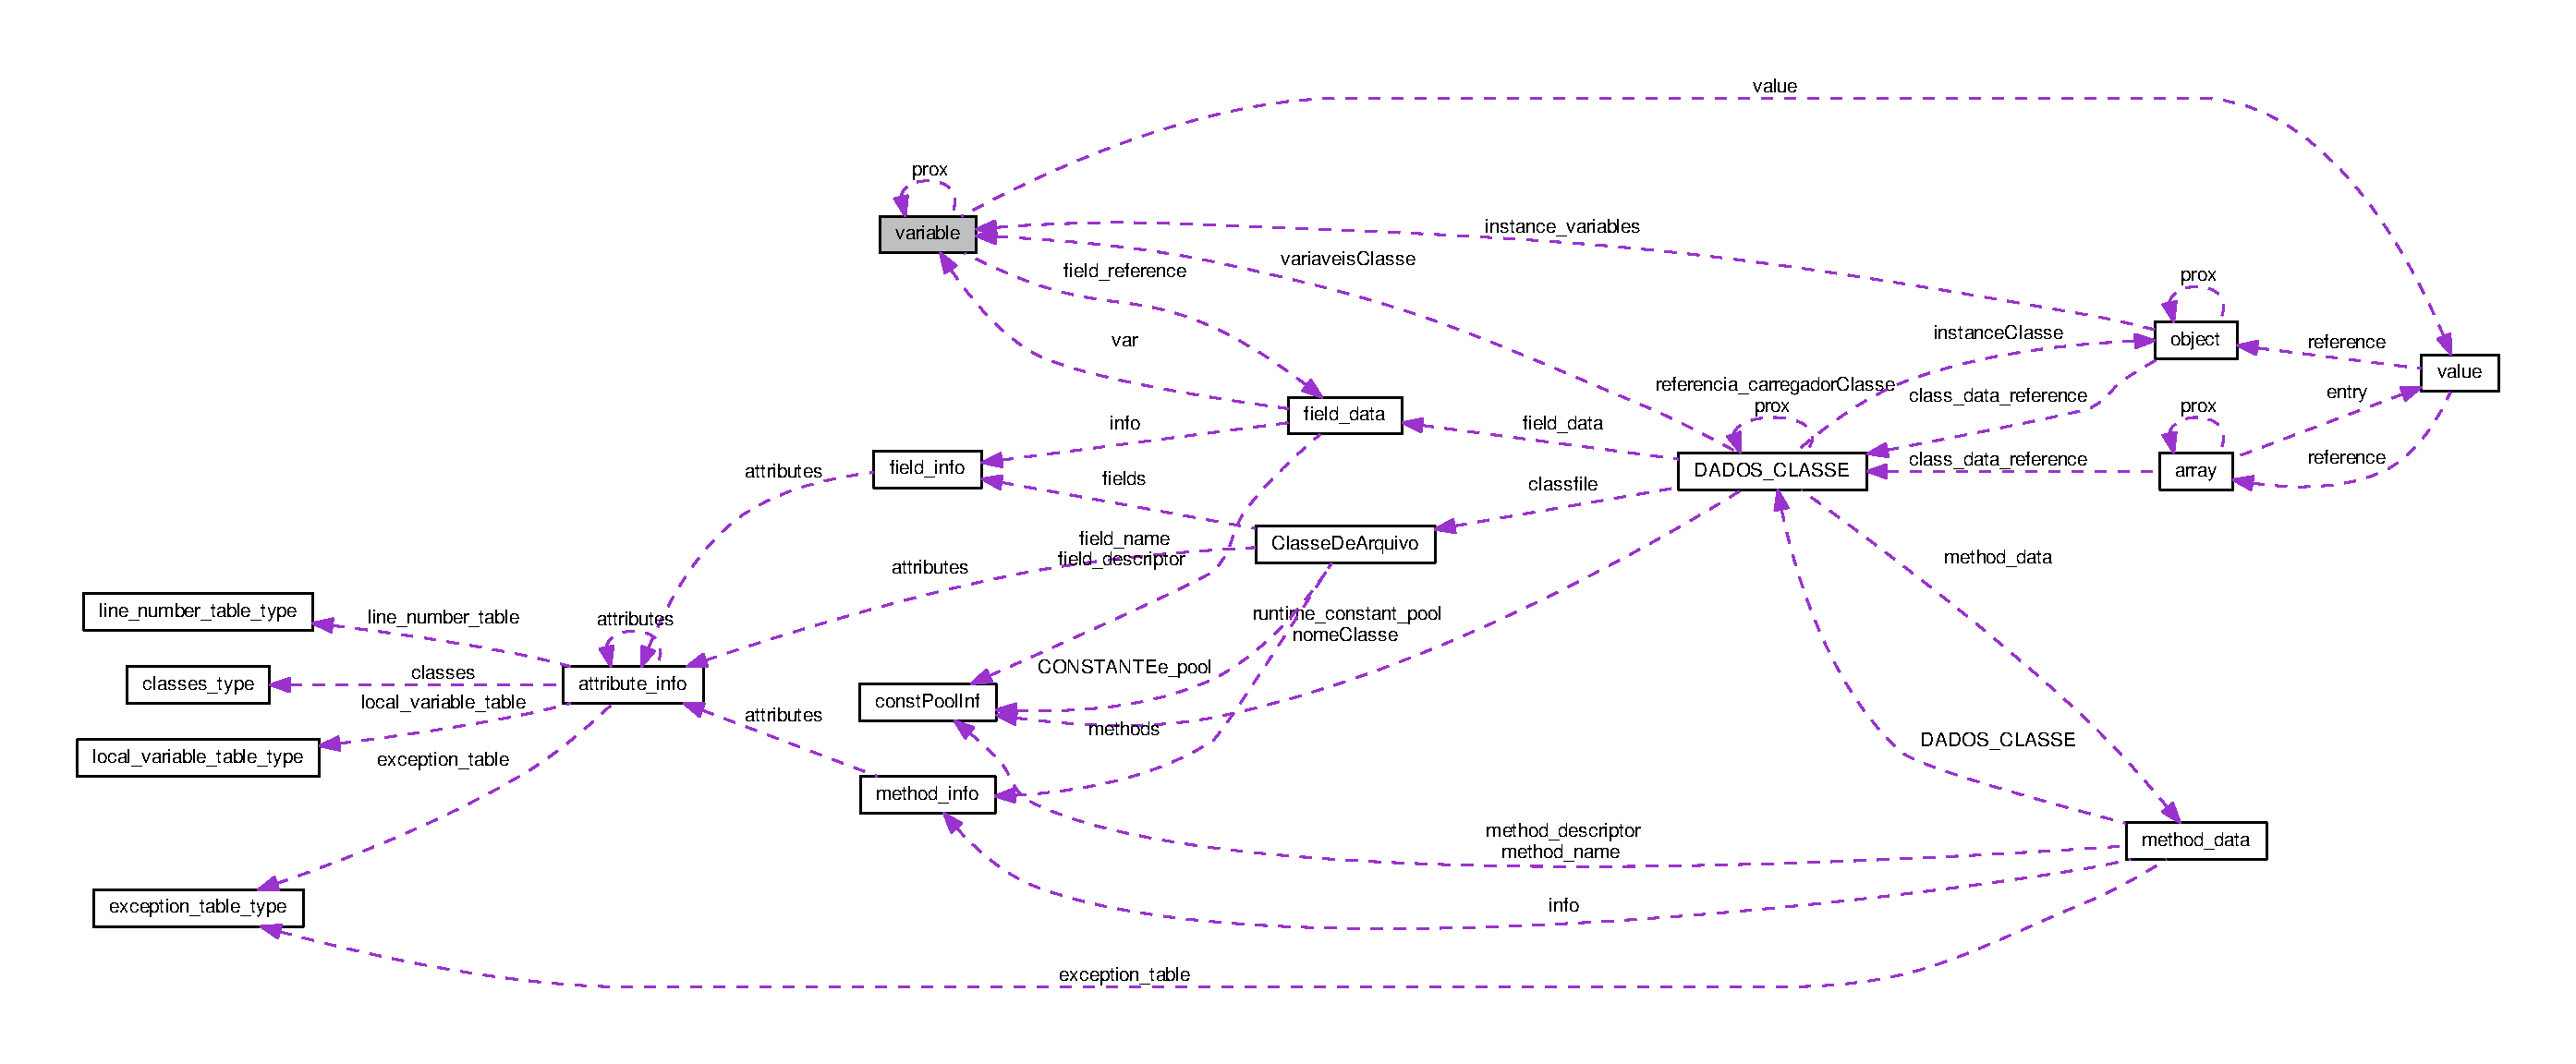
\includegraphics[width=350pt]{structvariable__coll__graph}
\end{center}
\end{figure}
\subsection*{Atributos Públicos}
\begin{DoxyCompactItemize}
\item 
\hyperlink{core_8h_ad5537b62ac62d6b7f34e2303f2b84982}{F\-I\-E\-L\-D\-\_\-\-D\-A\-T\-A} $\ast$ \hyperlink{structvariable_a49911b2c89f7f4e785091675963a3cbd}{field\-\_\-reference}
\item 
\hyperlink{core_8h_ad5d0e2bb91a9e28f920452e088b6462b}{V\-A\-L\-U\-E} \hyperlink{structvariable_a163435f346185d4f2d8d05a78dde5bef}{value}
\item 
struct \hyperlink{structvariable}{variable} $\ast$ \hyperlink{structvariable_aac55069e8378041cc5049f83410d1b5d}{prox}
\end{DoxyCompactItemize}


\subsection{Descrição detalhada}


Definido na linha 133 do ficheiro core.\-h.



\subsection{Documentação dos dados membro}
\hypertarget{structvariable_a49911b2c89f7f4e785091675963a3cbd}{\index{variable@{variable}!field\-\_\-reference@{field\-\_\-reference}}
\index{field\-\_\-reference@{field\-\_\-reference}!variable@{variable}}
\subsubsection[{field\-\_\-reference}]{\setlength{\rightskip}{0pt plus 5cm}{\bf F\-I\-E\-L\-D\-\_\-\-D\-A\-T\-A}$\ast$ variable\-::field\-\_\-reference}}\label{structvariable_a49911b2c89f7f4e785091675963a3cbd}


Definido na linha 134 do ficheiro core.\-h.

\hypertarget{structvariable_aac55069e8378041cc5049f83410d1b5d}{\index{variable@{variable}!prox@{prox}}
\index{prox@{prox}!variable@{variable}}
\subsubsection[{prox}]{\setlength{\rightskip}{0pt plus 5cm}struct {\bf variable}$\ast$ variable\-::prox}}\label{structvariable_aac55069e8378041cc5049f83410d1b5d}


Definido na linha 136 do ficheiro core.\-h.

\hypertarget{structvariable_a163435f346185d4f2d8d05a78dde5bef}{\index{variable@{variable}!value@{value}}
\index{value@{value}!variable@{variable}}
\subsubsection[{value}]{\setlength{\rightskip}{0pt plus 5cm}{\bf V\-A\-L\-U\-E} variable\-::value}}\label{structvariable_a163435f346185d4f2d8d05a78dde5bef}


Definido na linha 135 do ficheiro core.\-h.



A documentação para esta estrutura foi gerada a partir do seguinte ficheiro\-:\begin{DoxyCompactItemize}
\item 
\hyperlink{core_8h}{core.\-h}\end{DoxyCompactItemize}

\chapter{Documentação do ficheiro}
\hypertarget{checker_8c}{\section{Referência ao ficheiro checker.\-c}
\label{checker_8c}\index{checker.\-c@{checker.\-c}}
}
{\ttfamily \#include \char`\"{}checker.\-h\char`\"{}}\\*
Diagrama de dependências de inclusão para checker.\-c\-:
\nopagebreak
\begin{figure}[H]
\begin{center}
\leavevmode
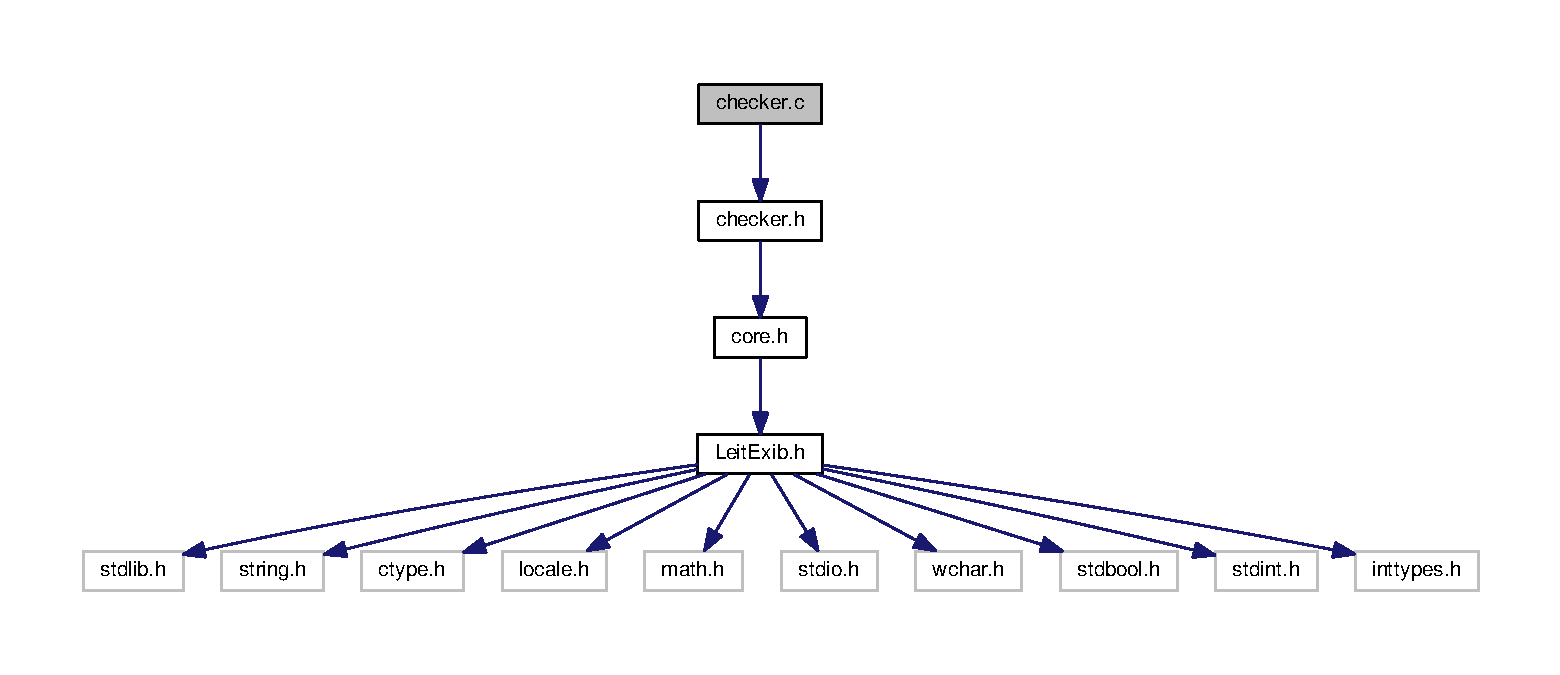
\includegraphics[width=350pt]{checker_8c__incl}
\end{center}
\end{figure}
\subsection*{Funções}
\begin{DoxyCompactItemize}
\item 
bool \hyperlink{checker_8c_ac5b6a6c9fa38ec400a3d15f1421089d8}{is\-Field\-Descriptor} (\hyperlink{structconst_pool_inf}{const\-Pool\-Inf} $\ast$cp, uint16\-\_\-t index)
\item 
bool \hyperlink{checker_8c_a9022e1fcb1064556f8df87f06b5babd2}{is\-Method\-Descriptor} (\hyperlink{structconst_pool_inf}{const\-Pool\-Inf} $\ast$cp, uint16\-\_\-t index)
\item 
void \hyperlink{checker_8c_a6ecc7358598704e5b4e9d77f06495482}{verify\-Constant\-Pool} (\hyperlink{struct_classe_de_arquivo}{Classe\-De\-Arquivo} $\ast$cf)
\item 
void \hyperlink{checker_8c_a3e295f32f754594e38f31297afebca97}{verify\-Access\-Flags} (\hyperlink{struct_classe_de_arquivo}{Classe\-De\-Arquivo} $\ast$cf)
\item 
void \hyperlink{checker_8c_a5c524d6b071cd201765ed95b10b9eedd}{verify\-Bytecode} (\hyperlink{structattribute__info}{attribute\-\_\-info} $\ast$attr, \hyperlink{struct_classe_de_arquivo}{Classe\-De\-Arquivo} $\ast$cf)
\item 
void \hyperlink{checker_8c_a0dcac7578c8c1cf7ef0f7b6fffe5ae24}{verify\-Classfile} (\hyperlink{struct_classe_de_arquivo}{Classe\-De\-Arquivo} $\ast$cf)
\item 
void \hyperlink{checker_8c_a7b952615631393d4b96a3eafe88cb3e7}{verify\-Super\-Final} (\hyperlink{struct_classe_de_arquivo}{Classe\-De\-Arquivo} $\ast$cf, \hyperlink{core_8h_a98bdb4b2c8aa49ba6bcd37df96469137}{J\-V\-M} $\ast$\hyperlink{structjvm}{jvm})
\item 
void \hyperlink{checker_8c_a4bbffc69c6cd821aebc4c480ffd3aec1}{verify\-Override\-Method\-Final} (\hyperlink{struct_classe_de_arquivo}{Classe\-De\-Arquivo} $\ast$cf, \hyperlink{core_8h_a98bdb4b2c8aa49ba6bcd37df96469137}{J\-V\-M} $\ast$\hyperlink{structjvm}{jvm})
\end{DoxyCompactItemize}


\subsection{Documentação das funções}
\hypertarget{checker_8c_ac5b6a6c9fa38ec400a3d15f1421089d8}{\index{checker.\-c@{checker.\-c}!is\-Field\-Descriptor@{is\-Field\-Descriptor}}
\index{is\-Field\-Descriptor@{is\-Field\-Descriptor}!checker.c@{checker.\-c}}
\subsubsection[{is\-Field\-Descriptor}]{\setlength{\rightskip}{0pt plus 5cm}bool is\-Field\-Descriptor (
\begin{DoxyParamCaption}
\item[{{\bf const\-Pool\-Inf} $\ast$}]{cp, }
\item[{uint16\-\_\-t}]{index}
\end{DoxyParamCaption}
)}}\label{checker_8c_ac5b6a6c9fa38ec400a3d15f1421089d8}


Definido na linha 5 do ficheiro checker.\-c.



Grafo de chamadas desta função\-:\nopagebreak
\begin{figure}[H]
\begin{center}
\leavevmode
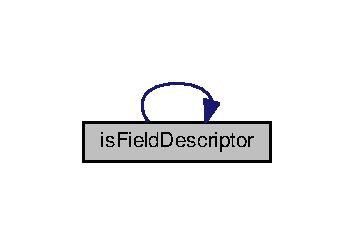
\includegraphics[width=170pt]{checker_8c_ac5b6a6c9fa38ec400a3d15f1421089d8_cgraph}
\end{center}
\end{figure}




Este é o diagrama das funções que utilizam esta função\-:
\nopagebreak
\begin{figure}[H]
\begin{center}
\leavevmode
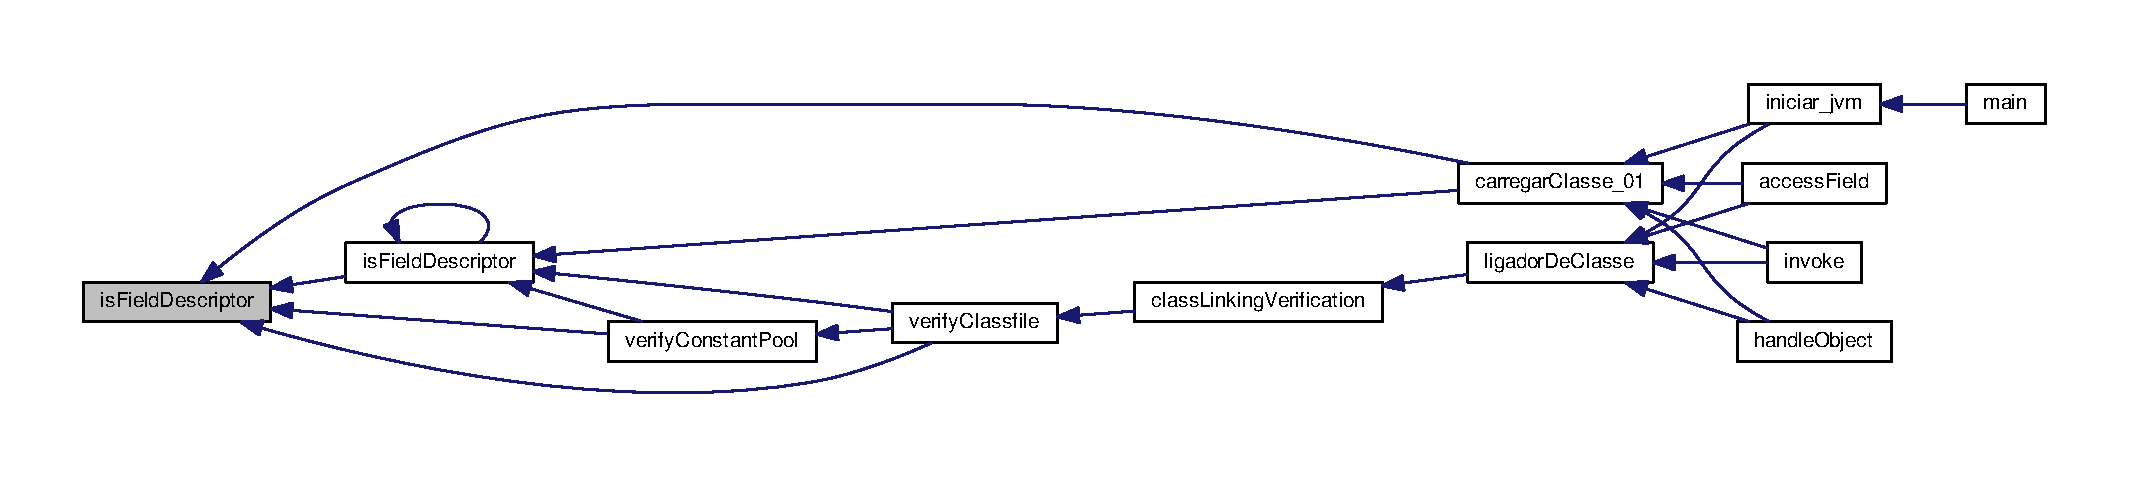
\includegraphics[width=350pt]{checker_8c_ac5b6a6c9fa38ec400a3d15f1421089d8_icgraph}
\end{center}
\end{figure}


\hypertarget{checker_8c_a9022e1fcb1064556f8df87f06b5babd2}{\index{checker.\-c@{checker.\-c}!is\-Method\-Descriptor@{is\-Method\-Descriptor}}
\index{is\-Method\-Descriptor@{is\-Method\-Descriptor}!checker.c@{checker.\-c}}
\subsubsection[{is\-Method\-Descriptor}]{\setlength{\rightskip}{0pt plus 5cm}bool is\-Method\-Descriptor (
\begin{DoxyParamCaption}
\item[{{\bf const\-Pool\-Inf} $\ast$}]{cp, }
\item[{uint16\-\_\-t}]{index}
\end{DoxyParamCaption}
)}}\label{checker_8c_a9022e1fcb1064556f8df87f06b5babd2}


Definido na linha 42 do ficheiro checker.\-c.



Grafo de chamadas desta função\-:\nopagebreak
\begin{figure}[H]
\begin{center}
\leavevmode
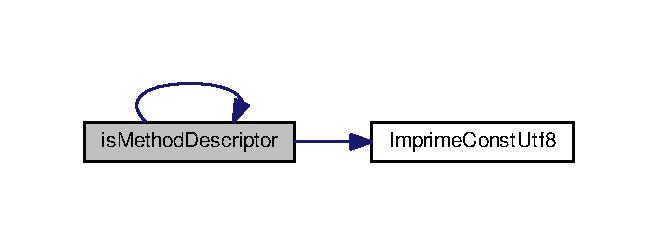
\includegraphics[width=316pt]{checker_8c_a9022e1fcb1064556f8df87f06b5babd2_cgraph}
\end{center}
\end{figure}




Este é o diagrama das funções que utilizam esta função\-:
\nopagebreak
\begin{figure}[H]
\begin{center}
\leavevmode
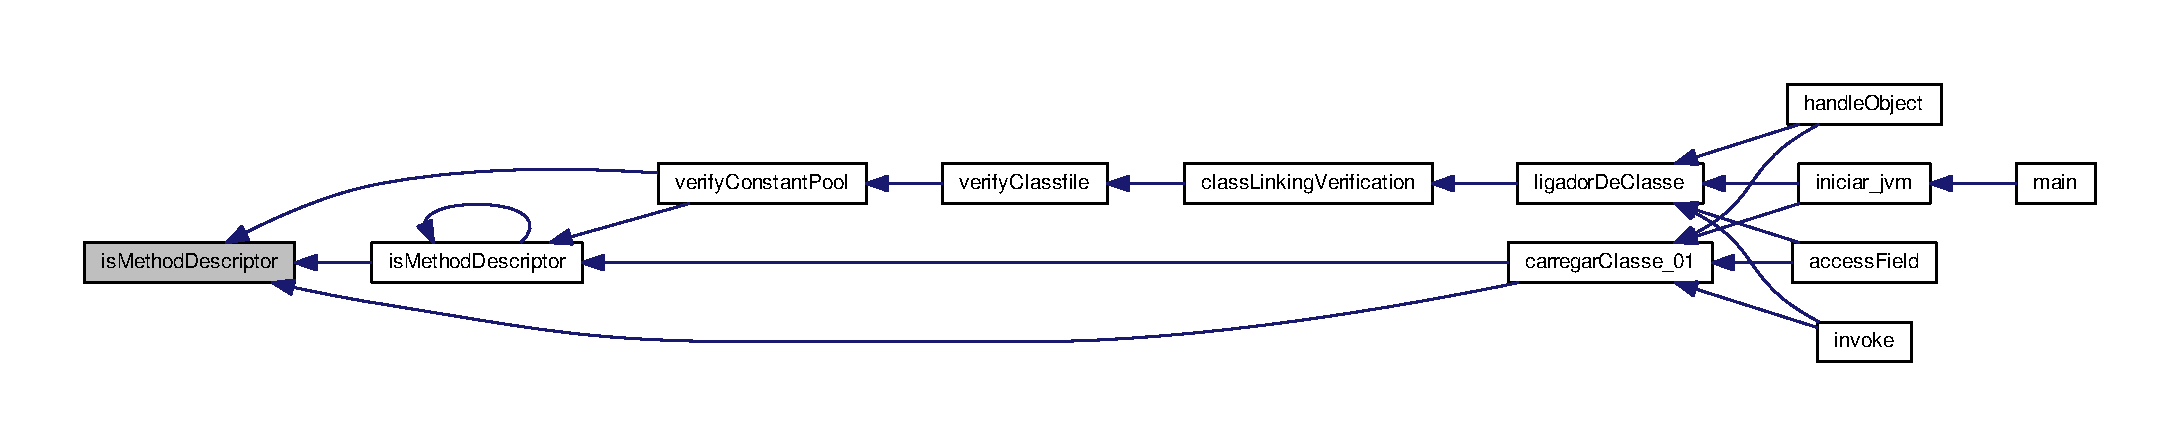
\includegraphics[width=350pt]{checker_8c_a9022e1fcb1064556f8df87f06b5babd2_icgraph}
\end{center}
\end{figure}


\hypertarget{checker_8c_a3e295f32f754594e38f31297afebca97}{\index{checker.\-c@{checker.\-c}!verify\-Access\-Flags@{verify\-Access\-Flags}}
\index{verify\-Access\-Flags@{verify\-Access\-Flags}!checker.c@{checker.\-c}}
\subsubsection[{verify\-Access\-Flags}]{\setlength{\rightskip}{0pt plus 5cm}void verify\-Access\-Flags (
\begin{DoxyParamCaption}
\item[{{\bf Classe\-De\-Arquivo} $\ast$}]{cf}
\end{DoxyParamCaption}
)}}\label{checker_8c_a3e295f32f754594e38f31297afebca97}


Definido na linha 268 do ficheiro checker.\-c.



Este é o diagrama das funções que utilizam esta função\-:
\nopagebreak
\begin{figure}[H]
\begin{center}
\leavevmode
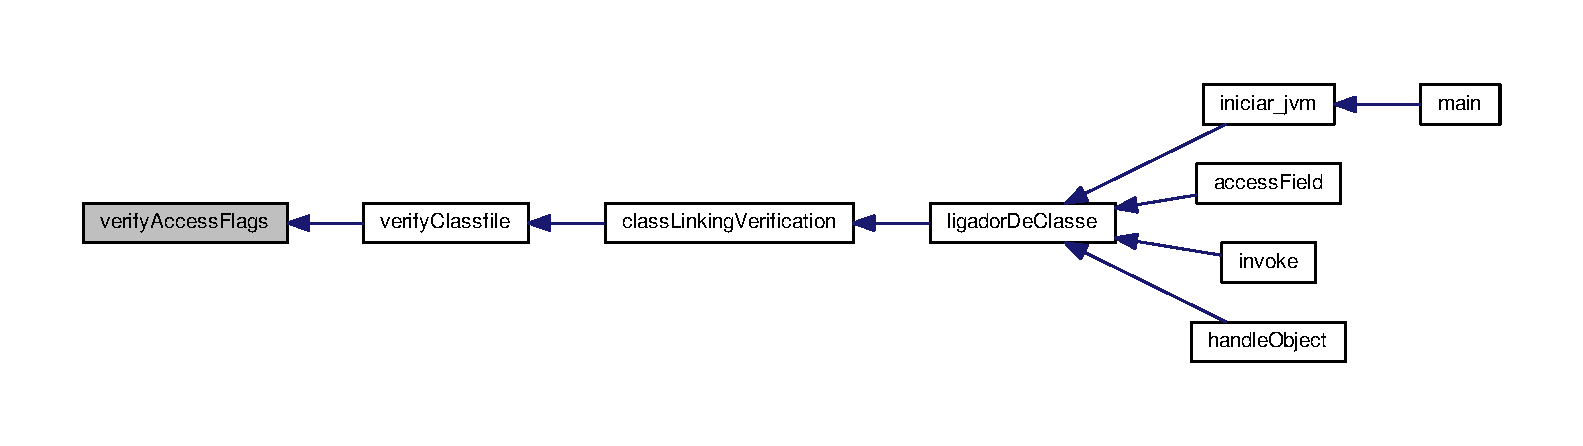
\includegraphics[width=350pt]{checker_8c_a3e295f32f754594e38f31297afebca97_icgraph}
\end{center}
\end{figure}


\hypertarget{checker_8c_a5c524d6b071cd201765ed95b10b9eedd}{\index{checker.\-c@{checker.\-c}!verify\-Bytecode@{verify\-Bytecode}}
\index{verify\-Bytecode@{verify\-Bytecode}!checker.c@{checker.\-c}}
\subsubsection[{verify\-Bytecode}]{\setlength{\rightskip}{0pt plus 5cm}void verify\-Bytecode (
\begin{DoxyParamCaption}
\item[{{\bf attribute\-\_\-info} $\ast$}]{attr, }
\item[{{\bf Classe\-De\-Arquivo} $\ast$}]{cf}
\end{DoxyParamCaption}
)}}\label{checker_8c_a5c524d6b071cd201765ed95b10b9eedd}


Definido na linha 299 do ficheiro checker.\-c.



Este é o diagrama das funções que utilizam esta função\-:
\nopagebreak
\begin{figure}[H]
\begin{center}
\leavevmode
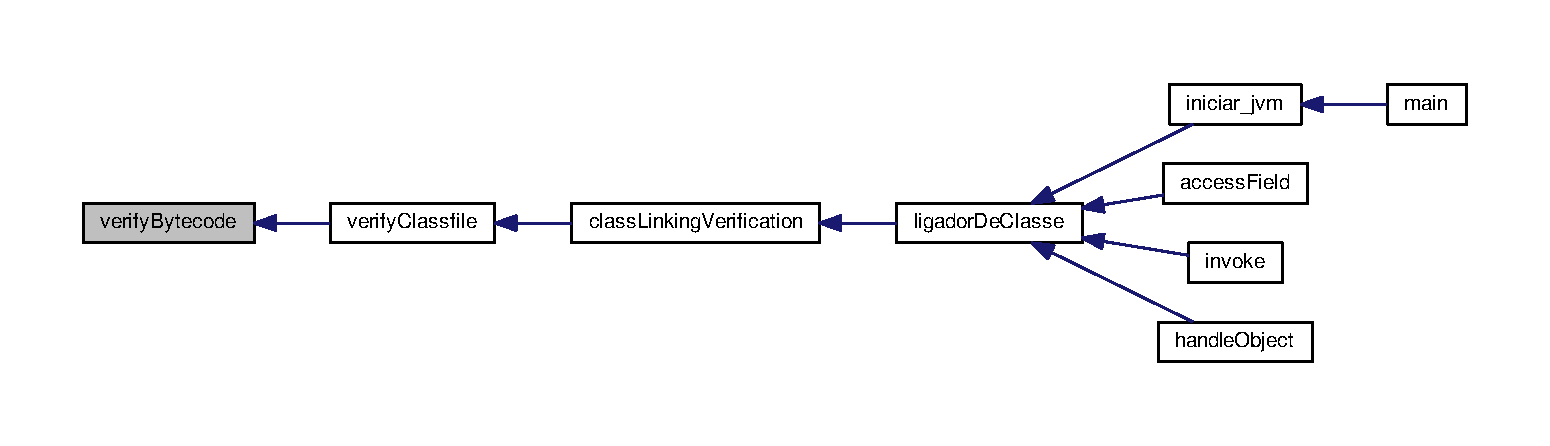
\includegraphics[width=350pt]{checker_8c_a5c524d6b071cd201765ed95b10b9eedd_icgraph}
\end{center}
\end{figure}


\hypertarget{checker_8c_a0dcac7578c8c1cf7ef0f7b6fffe5ae24}{\index{checker.\-c@{checker.\-c}!verify\-Classfile@{verify\-Classfile}}
\index{verify\-Classfile@{verify\-Classfile}!checker.c@{checker.\-c}}
\subsubsection[{verify\-Classfile}]{\setlength{\rightskip}{0pt plus 5cm}void verify\-Classfile (
\begin{DoxyParamCaption}
\item[{{\bf Classe\-De\-Arquivo} $\ast$}]{cf}
\end{DoxyParamCaption}
)}}\label{checker_8c_a0dcac7578c8c1cf7ef0f7b6fffe5ae24}


Definido na linha 330 do ficheiro checker.\-c.



Grafo de chamadas desta função\-:\nopagebreak
\begin{figure}[H]
\begin{center}
\leavevmode
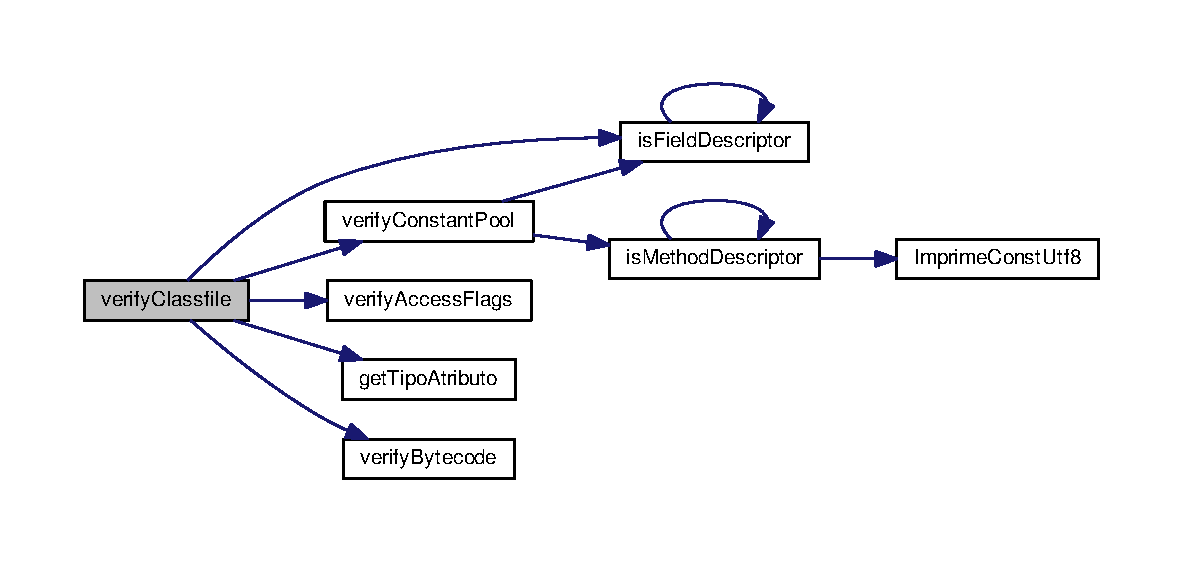
\includegraphics[width=350pt]{checker_8c_a0dcac7578c8c1cf7ef0f7b6fffe5ae24_cgraph}
\end{center}
\end{figure}




Este é o diagrama das funções que utilizam esta função\-:
\nopagebreak
\begin{figure}[H]
\begin{center}
\leavevmode
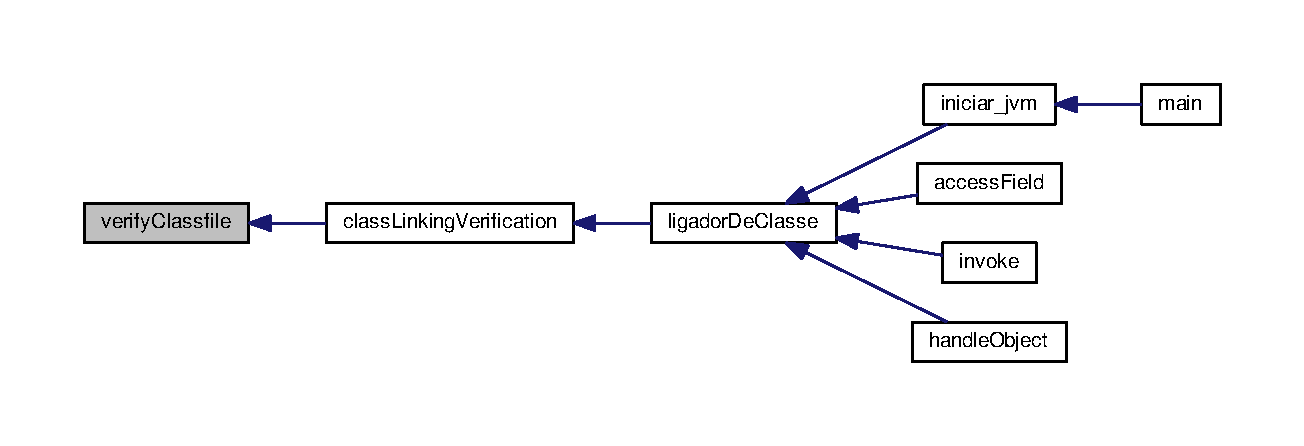
\includegraphics[width=350pt]{checker_8c_a0dcac7578c8c1cf7ef0f7b6fffe5ae24_icgraph}
\end{center}
\end{figure}


\hypertarget{checker_8c_a6ecc7358598704e5b4e9d77f06495482}{\index{checker.\-c@{checker.\-c}!verify\-Constant\-Pool@{verify\-Constant\-Pool}}
\index{verify\-Constant\-Pool@{verify\-Constant\-Pool}!checker.c@{checker.\-c}}
\subsubsection[{verify\-Constant\-Pool}]{\setlength{\rightskip}{0pt plus 5cm}void verify\-Constant\-Pool (
\begin{DoxyParamCaption}
\item[{{\bf Classe\-De\-Arquivo} $\ast$}]{cf}
\end{DoxyParamCaption}
)}}\label{checker_8c_a6ecc7358598704e5b4e9d77f06495482}


Definido na linha 130 do ficheiro checker.\-c.



Grafo de chamadas desta função\-:\nopagebreak
\begin{figure}[H]
\begin{center}
\leavevmode
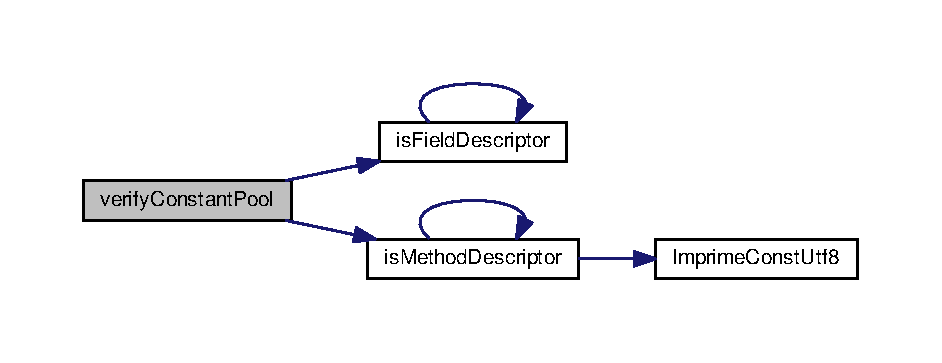
\includegraphics[width=350pt]{checker_8c_a6ecc7358598704e5b4e9d77f06495482_cgraph}
\end{center}
\end{figure}




Este é o diagrama das funções que utilizam esta função\-:
\nopagebreak
\begin{figure}[H]
\begin{center}
\leavevmode
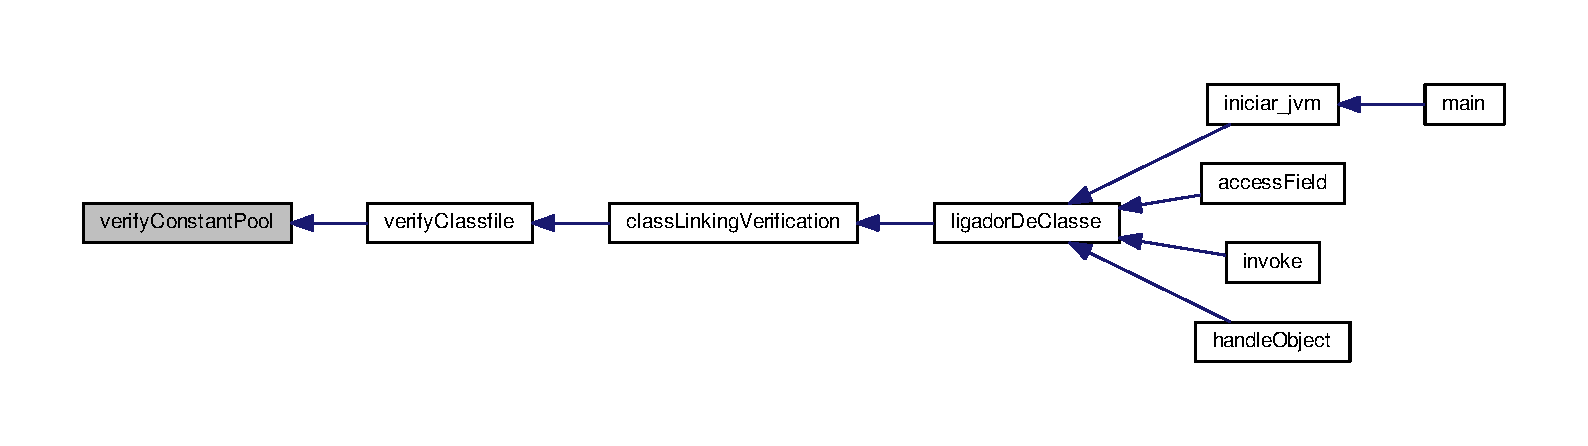
\includegraphics[width=350pt]{checker_8c_a6ecc7358598704e5b4e9d77f06495482_icgraph}
\end{center}
\end{figure}


\hypertarget{checker_8c_a4bbffc69c6cd821aebc4c480ffd3aec1}{\index{checker.\-c@{checker.\-c}!verify\-Override\-Method\-Final@{verify\-Override\-Method\-Final}}
\index{verify\-Override\-Method\-Final@{verify\-Override\-Method\-Final}!checker.c@{checker.\-c}}
\subsubsection[{verify\-Override\-Method\-Final}]{\setlength{\rightskip}{0pt plus 5cm}void verify\-Override\-Method\-Final (
\begin{DoxyParamCaption}
\item[{{\bf Classe\-De\-Arquivo} $\ast$}]{cf, }
\item[{{\bf J\-V\-M} $\ast$}]{jvm}
\end{DoxyParamCaption}
)}}\label{checker_8c_a4bbffc69c6cd821aebc4c480ffd3aec1}


Definido na linha 638 do ficheiro checker.\-c.



Grafo de chamadas desta função\-:\nopagebreak
\begin{figure}[H]
\begin{center}
\leavevmode
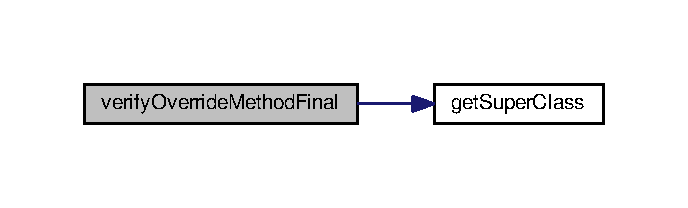
\includegraphics[width=330pt]{checker_8c_a4bbffc69c6cd821aebc4c480ffd3aec1_cgraph}
\end{center}
\end{figure}




Este é o diagrama das funções que utilizam esta função\-:
\nopagebreak
\begin{figure}[H]
\begin{center}
\leavevmode
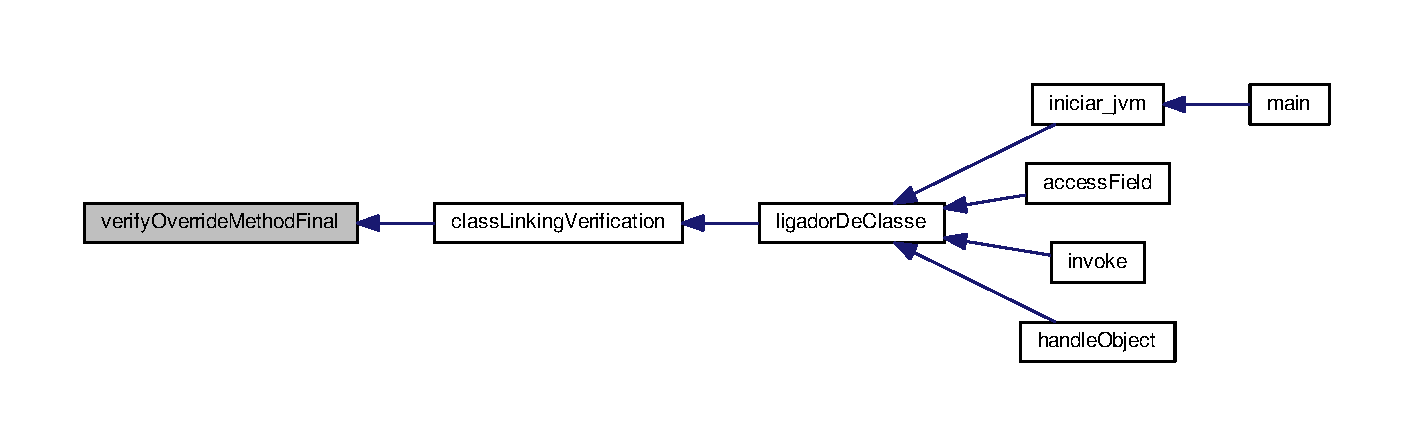
\includegraphics[width=350pt]{checker_8c_a4bbffc69c6cd821aebc4c480ffd3aec1_icgraph}
\end{center}
\end{figure}


\hypertarget{checker_8c_a7b952615631393d4b96a3eafe88cb3e7}{\index{checker.\-c@{checker.\-c}!verify\-Super\-Final@{verify\-Super\-Final}}
\index{verify\-Super\-Final@{verify\-Super\-Final}!checker.c@{checker.\-c}}
\subsubsection[{verify\-Super\-Final}]{\setlength{\rightskip}{0pt plus 5cm}void verify\-Super\-Final (
\begin{DoxyParamCaption}
\item[{{\bf Classe\-De\-Arquivo} $\ast$}]{cf, }
\item[{{\bf J\-V\-M} $\ast$}]{jvm}
\end{DoxyParamCaption}
)}}\label{checker_8c_a7b952615631393d4b96a3eafe88cb3e7}


Definido na linha 625 do ficheiro checker.\-c.



Grafo de chamadas desta função\-:\nopagebreak
\begin{figure}[H]
\begin{center}
\leavevmode
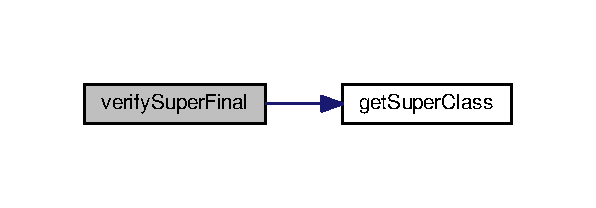
\includegraphics[width=286pt]{checker_8c_a7b952615631393d4b96a3eafe88cb3e7_cgraph}
\end{center}
\end{figure}




Este é o diagrama das funções que utilizam esta função\-:
\nopagebreak
\begin{figure}[H]
\begin{center}
\leavevmode
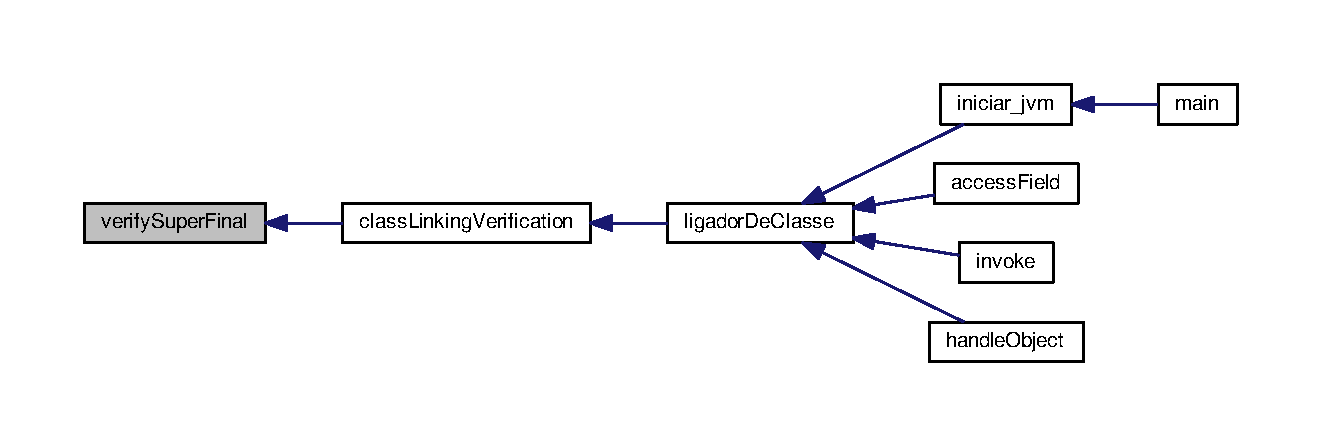
\includegraphics[width=350pt]{checker_8c_a7b952615631393d4b96a3eafe88cb3e7_icgraph}
\end{center}
\end{figure}



\hypertarget{checker_8h}{\section{Referência ao ficheiro checker.\-h}
\label{checker_8h}\index{checker.\-h@{checker.\-h}}
}
{\ttfamily \#include \char`\"{}core.\-h\char`\"{}}\\*
Diagrama de dependências de inclusão para checker.\-h\-:
\nopagebreak
\begin{figure}[H]
\begin{center}
\leavevmode
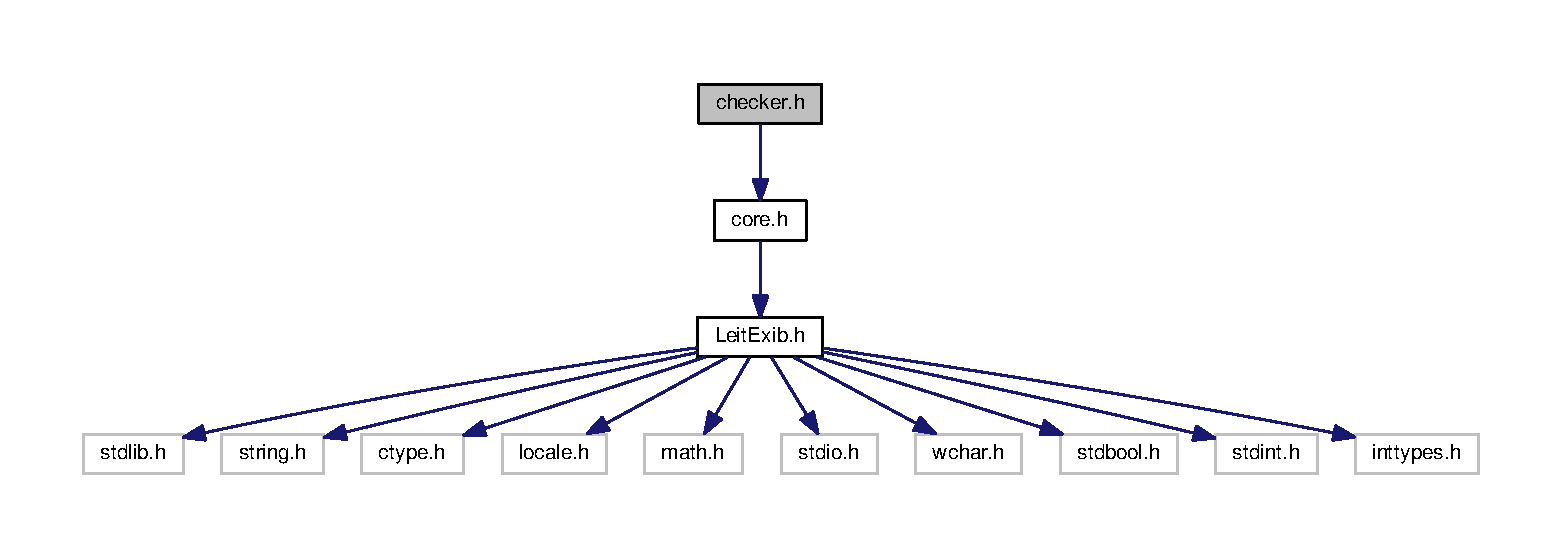
\includegraphics[width=350pt]{checker_8h__incl}
\end{center}
\end{figure}
Este grafo mostra quais são os ficheiros que incluem directamente ou indirectamente este ficheiro\-:\nopagebreak
\begin{figure}[H]
\begin{center}
\leavevmode
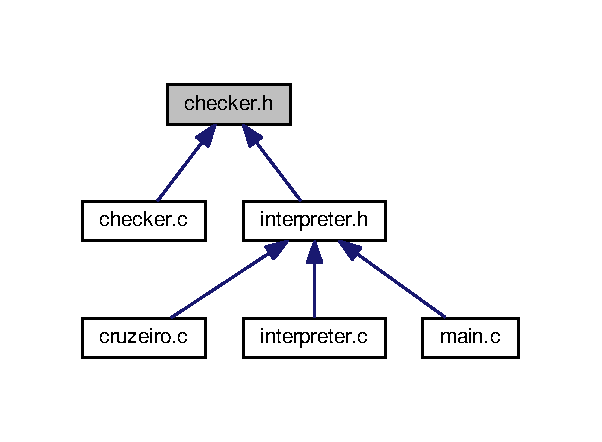
\includegraphics[width=289pt]{checker_8h__dep__incl}
\end{center}
\end{figure}
\subsection*{Funções}
\begin{DoxyCompactItemize}
\item 
bool \hyperlink{checker_8h_ae4f49d8a761fb2b65dd772afd027c3d6}{is\-Field\-Descriptor} (\hyperlink{structconst_pool_inf}{const\-Pool\-Inf} $\ast$, uint16\-\_\-t)
\item 
bool \hyperlink{checker_8h_affb083bf8031f48e5c478f976fcce70f}{is\-Method\-Descriptor} (\hyperlink{structconst_pool_inf}{const\-Pool\-Inf} $\ast$, uint16\-\_\-t)
\item 
void \hyperlink{checker_8h_ad1feb70bcfb835f9472fda62313ffbb6}{verify\-Constant\-Pool} (\hyperlink{struct_classe_de_arquivo}{Classe\-De\-Arquivo} $\ast$)
\item 
void \hyperlink{checker_8h_aad8e6070923c46681f8b2144b70c789a}{verify\-Access\-Flags} (\hyperlink{struct_classe_de_arquivo}{Classe\-De\-Arquivo} $\ast$)
\item 
void \hyperlink{checker_8h_a85b7fdf6ca41f7ae066becc961a2892b}{verify\-Bytecode} (\hyperlink{structattribute__info}{attribute\-\_\-info} $\ast$, \hyperlink{struct_classe_de_arquivo}{Classe\-De\-Arquivo} $\ast$)
\item 
void \hyperlink{checker_8h_a496eaab3cf87436d88f45f408fcc7b54}{verify\-Classfile} (\hyperlink{struct_classe_de_arquivo}{Classe\-De\-Arquivo} $\ast$)
\item 
void \hyperlink{checker_8h_aed60e642c76864b5b3b00950a8296a2d}{verify\-Super\-Final} (\hyperlink{struct_classe_de_arquivo}{Classe\-De\-Arquivo} $\ast$, \hyperlink{core_8h_a98bdb4b2c8aa49ba6bcd37df96469137}{J\-V\-M} $\ast$)
\item 
void \hyperlink{checker_8h_aeeaf21856554a50ea68bb1a9fcd69c2b}{verify\-Override\-Method\-Final} (\hyperlink{struct_classe_de_arquivo}{Classe\-De\-Arquivo} $\ast$, \hyperlink{core_8h_a98bdb4b2c8aa49ba6bcd37df96469137}{J\-V\-M} $\ast$)
\end{DoxyCompactItemize}


\subsection{Documentação das funções}
\hypertarget{checker_8h_ae4f49d8a761fb2b65dd772afd027c3d6}{\index{checker.\-h@{checker.\-h}!is\-Field\-Descriptor@{is\-Field\-Descriptor}}
\index{is\-Field\-Descriptor@{is\-Field\-Descriptor}!checker.h@{checker.\-h}}
\subsubsection[{is\-Field\-Descriptor}]{\setlength{\rightskip}{0pt plus 5cm}bool is\-Field\-Descriptor (
\begin{DoxyParamCaption}
\item[{{\bf const\-Pool\-Inf} $\ast$}]{, }
\item[{uint16\-\_\-t}]{}
\end{DoxyParamCaption}
)}}\label{checker_8h_ae4f49d8a761fb2b65dd772afd027c3d6}


Definido na linha 5 do ficheiro checker.\-c.



Grafo de chamadas desta função\-:\nopagebreak
\begin{figure}[H]
\begin{center}
\leavevmode
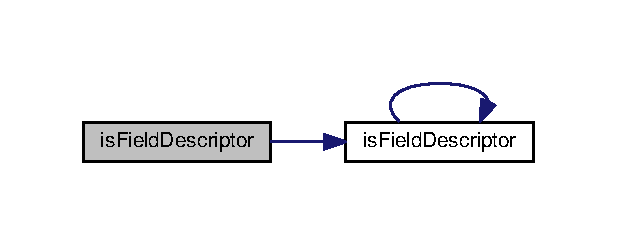
\includegraphics[width=296pt]{checker_8h_ae4f49d8a761fb2b65dd772afd027c3d6_cgraph}
\end{center}
\end{figure}




Este é o diagrama das funções que utilizam esta função\-:
\nopagebreak
\begin{figure}[H]
\begin{center}
\leavevmode
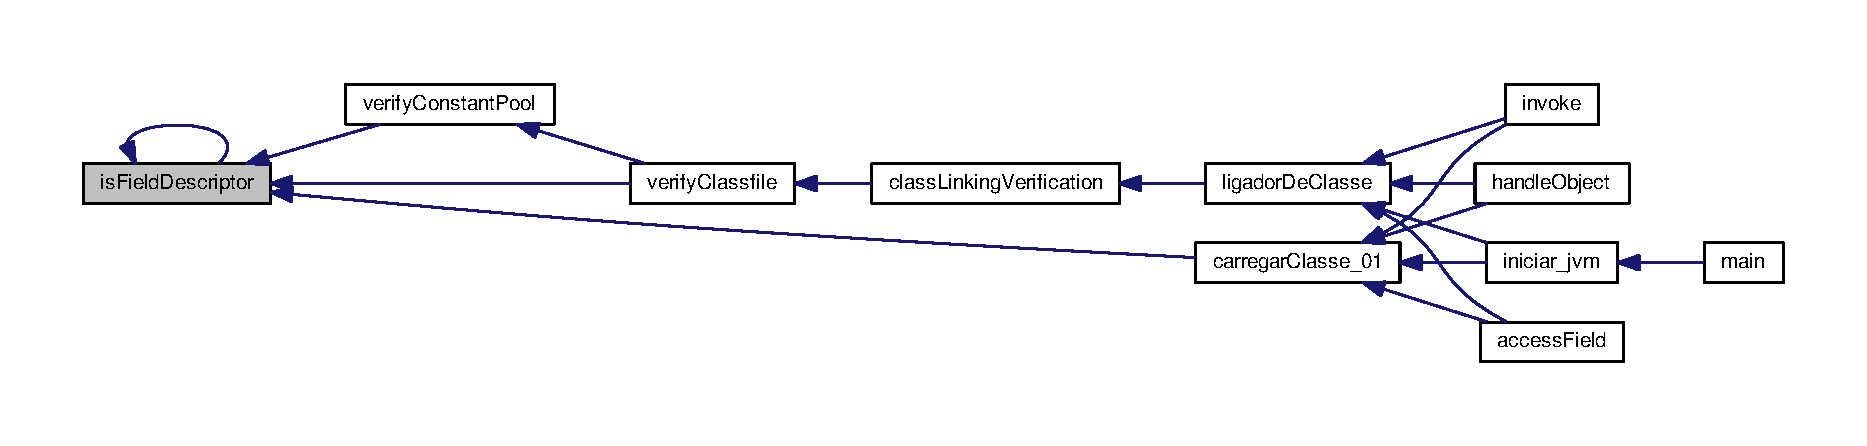
\includegraphics[width=350pt]{checker_8h_ae4f49d8a761fb2b65dd772afd027c3d6_icgraph}
\end{center}
\end{figure}


\hypertarget{checker_8h_affb083bf8031f48e5c478f976fcce70f}{\index{checker.\-h@{checker.\-h}!is\-Method\-Descriptor@{is\-Method\-Descriptor}}
\index{is\-Method\-Descriptor@{is\-Method\-Descriptor}!checker.h@{checker.\-h}}
\subsubsection[{is\-Method\-Descriptor}]{\setlength{\rightskip}{0pt plus 5cm}bool is\-Method\-Descriptor (
\begin{DoxyParamCaption}
\item[{{\bf const\-Pool\-Inf} $\ast$}]{, }
\item[{uint16\-\_\-t}]{}
\end{DoxyParamCaption}
)}}\label{checker_8h_affb083bf8031f48e5c478f976fcce70f}


Definido na linha 42 do ficheiro checker.\-c.



Grafo de chamadas desta função\-:\nopagebreak
\begin{figure}[H]
\begin{center}
\leavevmode
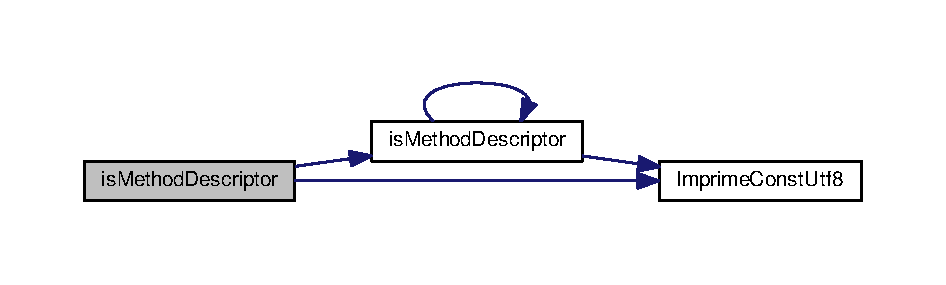
\includegraphics[width=350pt]{checker_8h_affb083bf8031f48e5c478f976fcce70f_cgraph}
\end{center}
\end{figure}




Este é o diagrama das funções que utilizam esta função\-:
\nopagebreak
\begin{figure}[H]
\begin{center}
\leavevmode
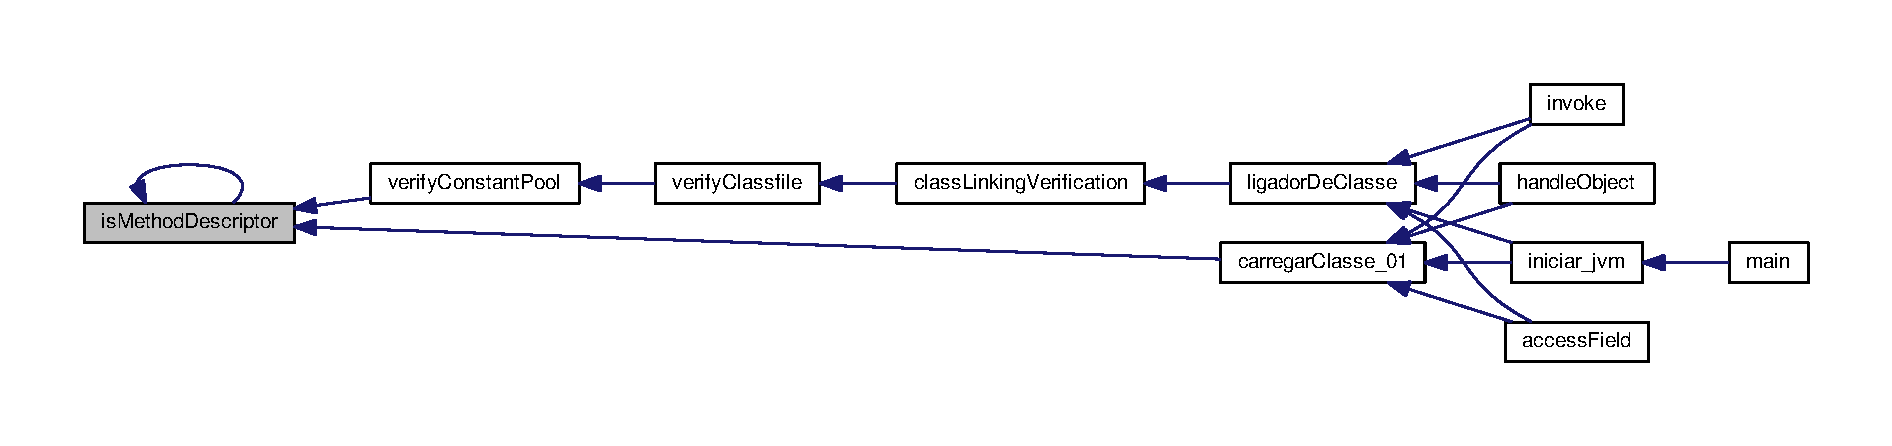
\includegraphics[width=350pt]{checker_8h_affb083bf8031f48e5c478f976fcce70f_icgraph}
\end{center}
\end{figure}


\hypertarget{checker_8h_aad8e6070923c46681f8b2144b70c789a}{\index{checker.\-h@{checker.\-h}!verify\-Access\-Flags@{verify\-Access\-Flags}}
\index{verify\-Access\-Flags@{verify\-Access\-Flags}!checker.h@{checker.\-h}}
\subsubsection[{verify\-Access\-Flags}]{\setlength{\rightskip}{0pt plus 5cm}void verify\-Access\-Flags (
\begin{DoxyParamCaption}
\item[{{\bf Classe\-De\-Arquivo} $\ast$}]{}
\end{DoxyParamCaption}
)}}\label{checker_8h_aad8e6070923c46681f8b2144b70c789a}


Definido na linha 268 do ficheiro checker.\-c.



Este é o diagrama das funções que utilizam esta função\-:
\nopagebreak
\begin{figure}[H]
\begin{center}
\leavevmode
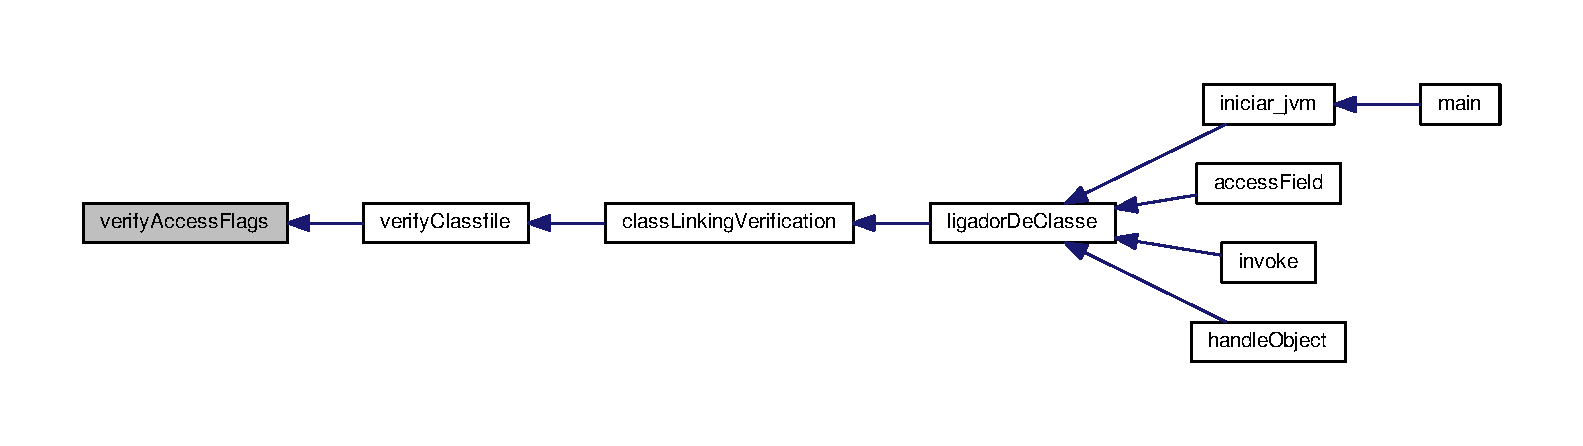
\includegraphics[width=350pt]{checker_8h_aad8e6070923c46681f8b2144b70c789a_icgraph}
\end{center}
\end{figure}


\hypertarget{checker_8h_a85b7fdf6ca41f7ae066becc961a2892b}{\index{checker.\-h@{checker.\-h}!verify\-Bytecode@{verify\-Bytecode}}
\index{verify\-Bytecode@{verify\-Bytecode}!checker.h@{checker.\-h}}
\subsubsection[{verify\-Bytecode}]{\setlength{\rightskip}{0pt plus 5cm}void verify\-Bytecode (
\begin{DoxyParamCaption}
\item[{{\bf attribute\-\_\-info} $\ast$}]{, }
\item[{{\bf Classe\-De\-Arquivo} $\ast$}]{}
\end{DoxyParamCaption}
)}}\label{checker_8h_a85b7fdf6ca41f7ae066becc961a2892b}


Definido na linha 299 do ficheiro checker.\-c.



Este é o diagrama das funções que utilizam esta função\-:
\nopagebreak
\begin{figure}[H]
\begin{center}
\leavevmode
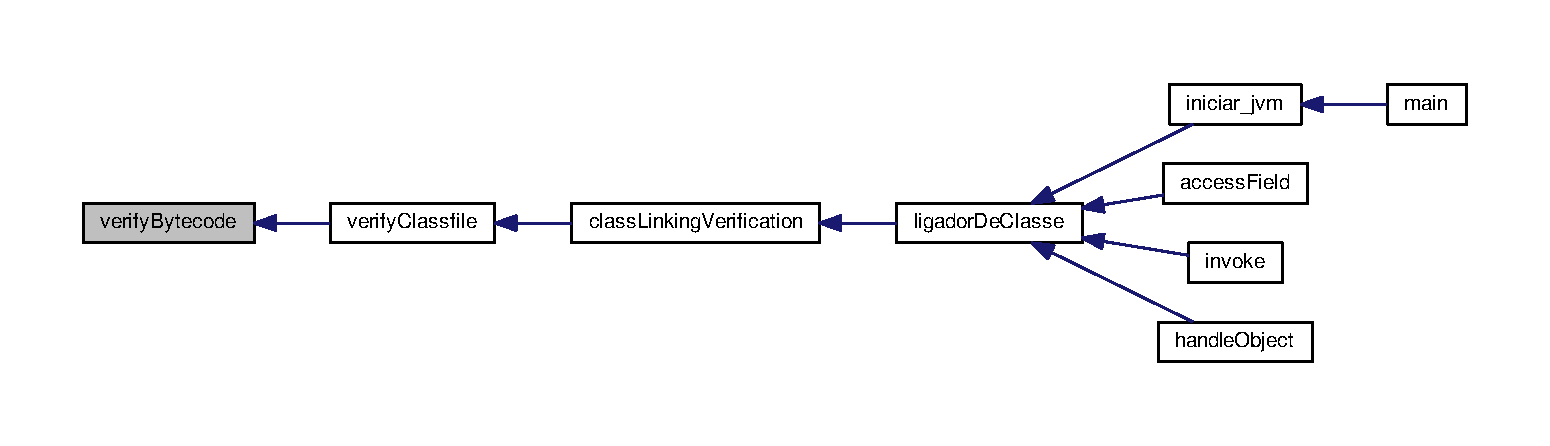
\includegraphics[width=350pt]{checker_8h_a85b7fdf6ca41f7ae066becc961a2892b_icgraph}
\end{center}
\end{figure}


\hypertarget{checker_8h_a496eaab3cf87436d88f45f408fcc7b54}{\index{checker.\-h@{checker.\-h}!verify\-Classfile@{verify\-Classfile}}
\index{verify\-Classfile@{verify\-Classfile}!checker.h@{checker.\-h}}
\subsubsection[{verify\-Classfile}]{\setlength{\rightskip}{0pt plus 5cm}void verify\-Classfile (
\begin{DoxyParamCaption}
\item[{{\bf Classe\-De\-Arquivo} $\ast$}]{}
\end{DoxyParamCaption}
)}}\label{checker_8h_a496eaab3cf87436d88f45f408fcc7b54}


Definido na linha 330 do ficheiro checker.\-c.



Grafo de chamadas desta função\-:\nopagebreak
\begin{figure}[H]
\begin{center}
\leavevmode
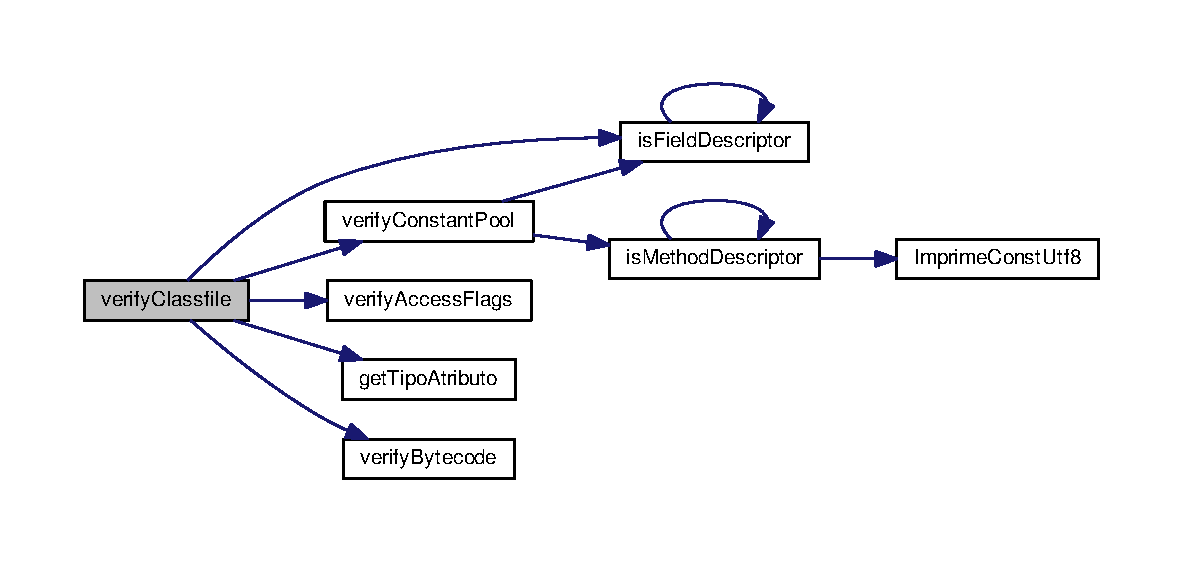
\includegraphics[width=350pt]{checker_8h_a496eaab3cf87436d88f45f408fcc7b54_cgraph}
\end{center}
\end{figure}




Este é o diagrama das funções que utilizam esta função\-:
\nopagebreak
\begin{figure}[H]
\begin{center}
\leavevmode
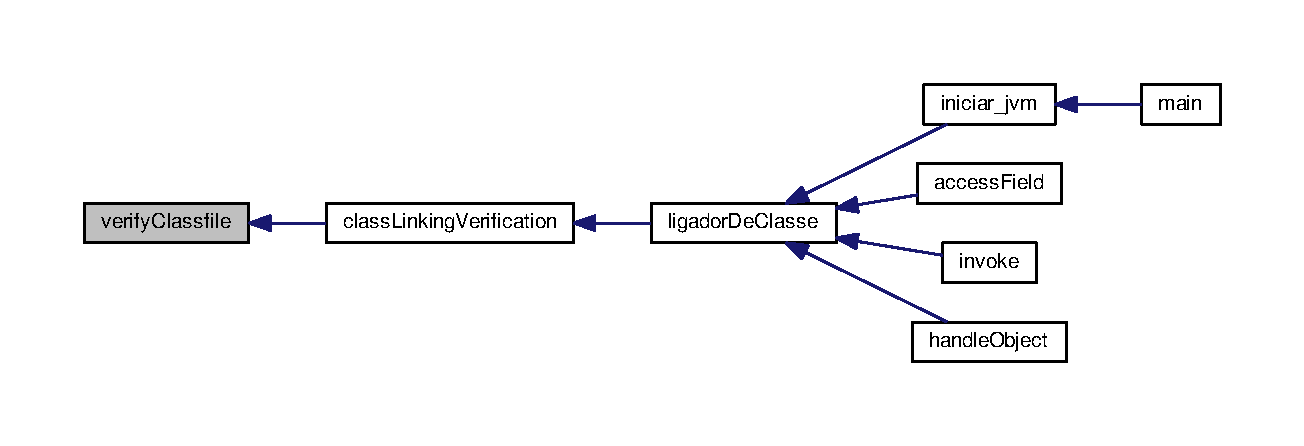
\includegraphics[width=350pt]{checker_8h_a496eaab3cf87436d88f45f408fcc7b54_icgraph}
\end{center}
\end{figure}


\hypertarget{checker_8h_ad1feb70bcfb835f9472fda62313ffbb6}{\index{checker.\-h@{checker.\-h}!verify\-Constant\-Pool@{verify\-Constant\-Pool}}
\index{verify\-Constant\-Pool@{verify\-Constant\-Pool}!checker.h@{checker.\-h}}
\subsubsection[{verify\-Constant\-Pool}]{\setlength{\rightskip}{0pt plus 5cm}void verify\-Constant\-Pool (
\begin{DoxyParamCaption}
\item[{{\bf Classe\-De\-Arquivo} $\ast$}]{}
\end{DoxyParamCaption}
)}}\label{checker_8h_ad1feb70bcfb835f9472fda62313ffbb6}


Definido na linha 130 do ficheiro checker.\-c.



Grafo de chamadas desta função\-:\nopagebreak
\begin{figure}[H]
\begin{center}
\leavevmode
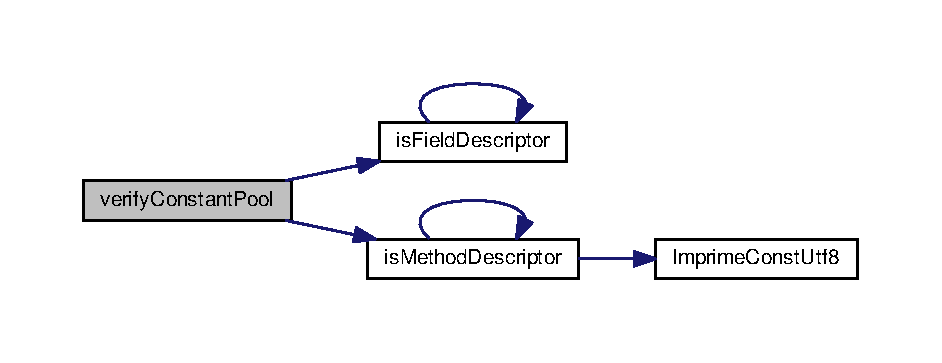
\includegraphics[width=350pt]{checker_8h_ad1feb70bcfb835f9472fda62313ffbb6_cgraph}
\end{center}
\end{figure}




Este é o diagrama das funções que utilizam esta função\-:
\nopagebreak
\begin{figure}[H]
\begin{center}
\leavevmode
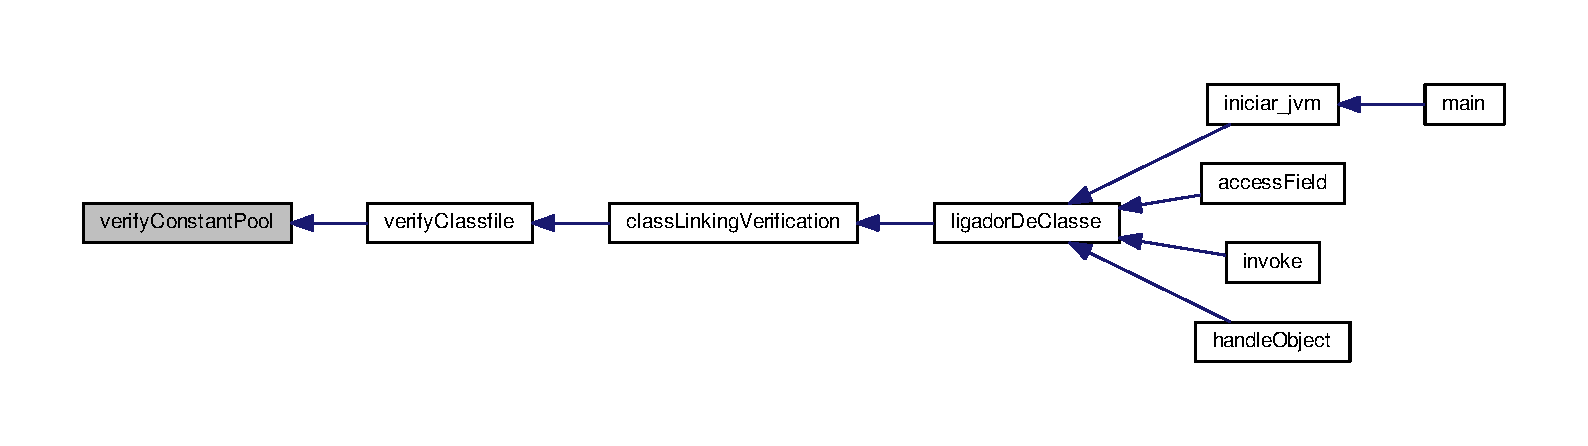
\includegraphics[width=350pt]{checker_8h_ad1feb70bcfb835f9472fda62313ffbb6_icgraph}
\end{center}
\end{figure}


\hypertarget{checker_8h_aeeaf21856554a50ea68bb1a9fcd69c2b}{\index{checker.\-h@{checker.\-h}!verify\-Override\-Method\-Final@{verify\-Override\-Method\-Final}}
\index{verify\-Override\-Method\-Final@{verify\-Override\-Method\-Final}!checker.h@{checker.\-h}}
\subsubsection[{verify\-Override\-Method\-Final}]{\setlength{\rightskip}{0pt plus 5cm}void verify\-Override\-Method\-Final (
\begin{DoxyParamCaption}
\item[{{\bf Classe\-De\-Arquivo} $\ast$}]{, }
\item[{{\bf J\-V\-M} $\ast$}]{}
\end{DoxyParamCaption}
)}}\label{checker_8h_aeeaf21856554a50ea68bb1a9fcd69c2b}


Definido na linha 638 do ficheiro checker.\-c.



Grafo de chamadas desta função\-:\nopagebreak
\begin{figure}[H]
\begin{center}
\leavevmode
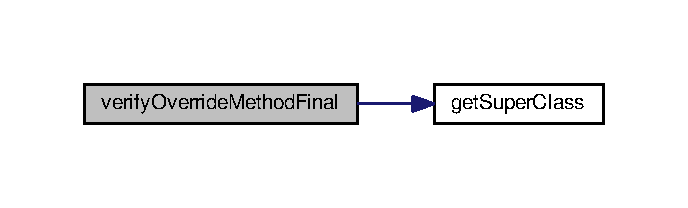
\includegraphics[width=330pt]{checker_8h_aeeaf21856554a50ea68bb1a9fcd69c2b_cgraph}
\end{center}
\end{figure}




Este é o diagrama das funções que utilizam esta função\-:
\nopagebreak
\begin{figure}[H]
\begin{center}
\leavevmode
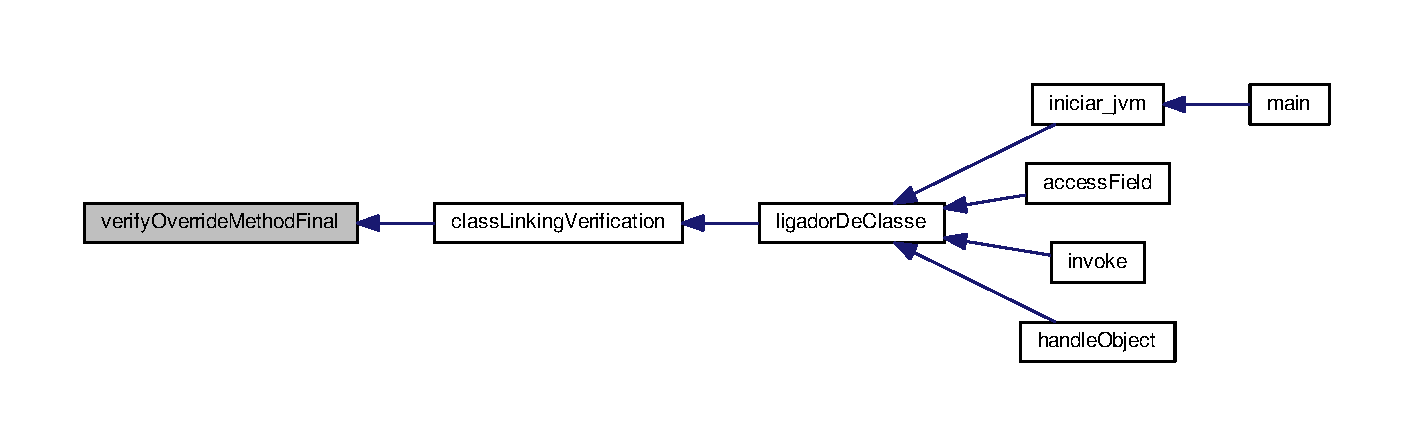
\includegraphics[width=350pt]{checker_8h_aeeaf21856554a50ea68bb1a9fcd69c2b_icgraph}
\end{center}
\end{figure}


\hypertarget{checker_8h_aed60e642c76864b5b3b00950a8296a2d}{\index{checker.\-h@{checker.\-h}!verify\-Super\-Final@{verify\-Super\-Final}}
\index{verify\-Super\-Final@{verify\-Super\-Final}!checker.h@{checker.\-h}}
\subsubsection[{verify\-Super\-Final}]{\setlength{\rightskip}{0pt plus 5cm}void verify\-Super\-Final (
\begin{DoxyParamCaption}
\item[{{\bf Classe\-De\-Arquivo} $\ast$}]{, }
\item[{{\bf J\-V\-M} $\ast$}]{}
\end{DoxyParamCaption}
)}}\label{checker_8h_aed60e642c76864b5b3b00950a8296a2d}


Definido na linha 625 do ficheiro checker.\-c.



Grafo de chamadas desta função\-:\nopagebreak
\begin{figure}[H]
\begin{center}
\leavevmode
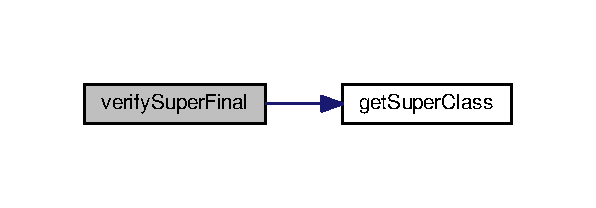
\includegraphics[width=286pt]{checker_8h_aed60e642c76864b5b3b00950a8296a2d_cgraph}
\end{center}
\end{figure}




Este é o diagrama das funções que utilizam esta função\-:
\nopagebreak
\begin{figure}[H]
\begin{center}
\leavevmode
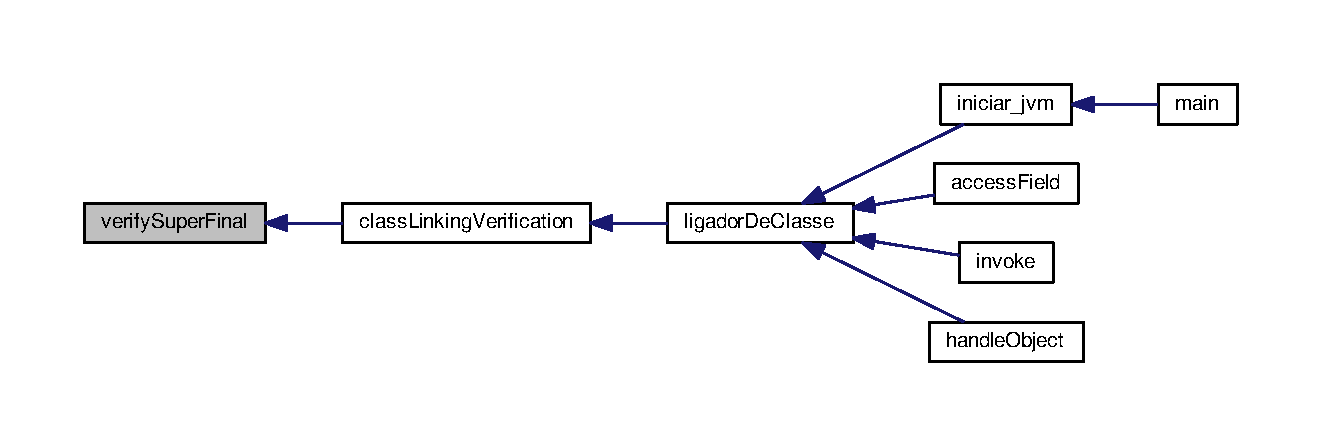
\includegraphics[width=350pt]{checker_8h_aed60e642c76864b5b3b00950a8296a2d_icgraph}
\end{center}
\end{figure}



\hypertarget{core_8h}{\section{Referência ao ficheiro core.\-h}
\label{core_8h}\index{core.\-h@{core.\-h}}
}
{\ttfamily \#include \char`\"{}Leit\-Exib.\-h\char`\"{}}\\*
Diagrama de dependências de inclusão para core.\-h\-:\nopagebreak
\begin{figure}[H]
\begin{center}
\leavevmode
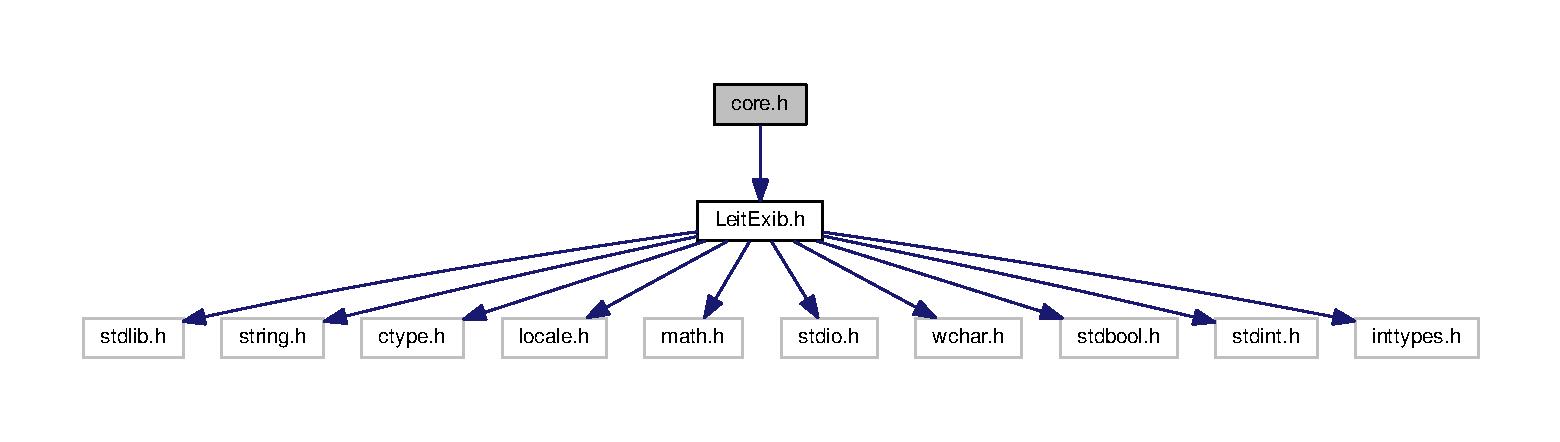
\includegraphics[width=350pt]{core_8h__incl}
\end{center}
\end{figure}
Este grafo mostra quais são os ficheiros que incluem directamente ou indirectamente este ficheiro\-:\nopagebreak
\begin{figure}[H]
\begin{center}
\leavevmode
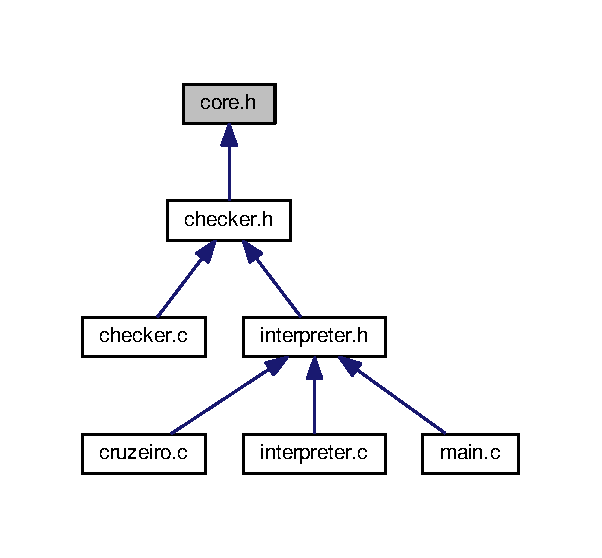
\includegraphics[width=289pt]{core_8h__dep__incl}
\end{center}
\end{figure}
\subsection*{Componentes}
\begin{DoxyCompactItemize}
\item 
struct \hyperlink{structvalue}{value}
\item 
struct \hyperlink{structoperand}{operand}
\item 
struct \hyperlink{structframe}{frame}
\item 
struct \hyperlink{structthread}{thread}
\item 
struct \hyperlink{structheap__area}{heap\-\_\-area}
\item 
struct \hyperlink{structfield__data}{field\-\_\-data}
\item 
struct \hyperlink{structvariable}{variable}
\item 
struct \hyperlink{structmethod__data}{method\-\_\-data}
\item 
struct \hyperlink{struct_d_a_d_o_s___c_l_a_s_s_e}{D\-A\-D\-O\-S\-\_\-\-C\-L\-A\-S\-S\-E}
\item 
struct \hyperlink{structobject}{object}
\item 
struct \hyperlink{structarray}{array}
\item 
struct \hyperlink{structjvm}{jvm}
\end{DoxyCompactItemize}
\subsection*{Macros}
\begin{DoxyCompactItemize}
\item 
\#define \hyperlink{core_8h_aec93e83855ac17c3c25c55c37ca186dd}{B\-Y\-T\-E}~'B'
\item 
\#define \hyperlink{core_8h_a35cd67ba7bb0db8105eb6267467535d7}{C\-H\-A\-R}~'C'
\item 
\#define \hyperlink{core_8h_a8747af38b86aa2bbcda2f1b1aa0888c2}{D\-O\-U\-B\-L\-E}~'D'
\item 
\#define \hyperlink{core_8h_ae8690abbffa85934d64d545920e2b108}{F\-L\-O\-A\-T}~'F'
\item 
\#define \hyperlink{core_8h_afeeffe52c8fd59db7c61cf8b02042dbf}{I\-N\-T}~'I'
\item 
\#define \hyperlink{core_8h_acaa7b8a7167a8214f499c71c413ddcca}{L\-O\-N\-G}~'J'
\item 
\#define \hyperlink{core_8h_abc89a525f57ec2bfb44ee9e48660154f}{R\-E\-F\-\_\-\-I\-N\-S\-T}~'L'
\item 
\#define \hyperlink{core_8h_a9fbb14850a9f176447733a089071cd70}{S\-H\-O\-R\-T}~'S'
\item 
\#define \hyperlink{core_8h_a50168fdbaa52d4a0b1c287d476050f12}{B\-O\-O\-L\-E\-A\-N}~'Z'
\item 
\#define \hyperlink{core_8h_a0fe85cdfdc6ac54e3d35b46683608dc4}{R\-E\-F\-\_\-\-A\-R\-R\-A\-Y}~'\mbox{[}'
\end{DoxyCompactItemize}
\subsection*{Definições de tipos}
\begin{DoxyCompactItemize}
\item 
typedef uint8\-\_\-t \hyperlink{core_8h_ab34056db44556fbb28ffa6aff4873b4c}{O\-P\-C\-O\-D\-E}
\item 
typedef char \hyperlink{core_8h_a96376f31c362e2a289072478449290f8}{T\-Y\-P\-E}
\item 
typedef uint32\-\_\-t \hyperlink{core_8h_aeeb4b41434914a6809f3448b40f818de}{A\-R\-R\-A\-Y\-\_\-\-T\-Y\-P\-E}
\item 
typedef struct \hyperlink{structobject}{object} \hyperlink{core_8h_a75cf109ba9d4518221445697fdbfc933}{obj}
\item 
typedef struct \hyperlink{structarray}{array} \hyperlink{core_8h_a96c64553ad75dd4c717e10b23fafaf1b}{ar}
\item 
typedef struct \hyperlink{structvalue}{value} \hyperlink{core_8h_ad5d0e2bb91a9e28f920452e088b6462b}{V\-A\-L\-U\-E}
\item 
typedef struct \hyperlink{structoperand}{operand} \hyperlink{core_8h_a57370c151bf2eefc3bd6e2d13b70e7c9}{O\-P\-E\-R\-A\-N\-D}
\item 
typedef struct \hyperlink{structframe}{frame} \hyperlink{core_8h_ad2c7f62ece09f452ea1a5285adcc503c}{F\-R\-A\-M\-E}
\item 
typedef struct \hyperlink{structthread}{thread} \hyperlink{core_8h_ad43b7ffe97b146f9dce917ae2a0fd181}{T\-H\-R\-E\-A\-D}
\item 
typedef struct \hyperlink{structheap__area}{heap\-\_\-area} \hyperlink{core_8h_a8aa4d8af3cc19c82a17fa714d533cb8f}{H\-E\-A\-P\-\_\-\-A\-R\-E\-A}
\item 
typedef struct \hyperlink{structfield__data}{field\-\_\-data} \hyperlink{core_8h_ad5537b62ac62d6b7f34e2303f2b84982}{F\-I\-E\-L\-D\-\_\-\-D\-A\-T\-A}
\item 
typedef struct \hyperlink{structvariable}{variable} \hyperlink{core_8h_a85b40991452ad00efae1784148c94402}{V\-A\-R\-I\-A\-B\-L\-E}
\item 
typedef struct \hyperlink{structmethod__data}{method\-\_\-data} \hyperlink{core_8h_af2592f49e52b0675aaca5850571f3999}{M\-E\-T\-H\-O\-D\-\_\-\-D\-A\-T\-A}
\item 
typedef struct \hyperlink{struct_d_a_d_o_s___c_l_a_s_s_e}{D\-A\-D\-O\-S\-\_\-\-C\-L\-A\-S\-S\-E} \hyperlink{core_8h_a116ede3eb3d97f03336302025379d1c7}{D\-A\-D\-O\-S\-\_\-\-C\-L\-A\-S\-S\-E}
\item 
typedef struct \hyperlink{structobject}{object} \hyperlink{core_8h_ae612e57be74359cf1e07ade2d61a86a0}{O\-B\-J\-E\-C\-T}
\item 
typedef struct \hyperlink{structarray}{array} \hyperlink{core_8h_a9c07c3330f66f4018e49ee90e58f0f39}{A\-R\-R\-A\-Y}
\item 
typedef struct \hyperlink{structjvm}{jvm} \hyperlink{core_8h_a98bdb4b2c8aa49ba6bcd37df96469137}{J\-V\-M}
\end{DoxyCompactItemize}
\subsection*{Funções}
\begin{DoxyCompactItemize}
\item 
void \hyperlink{core_8h_aa2f1283af56df2749e5702e0b569c5d7}{iniciar\-\_\-jvm} (char $\ast$, int, char $\ast$$\ast$)
\item 
void \hyperlink{core_8h_a7c9daf914ef558b41a9d0b2d617dab86}{carregar\-Classe\-\_\-01} (char $\ast$, \hyperlink{struct_d_a_d_o_s___c_l_a_s_s_e}{D\-A\-D\-O\-S\-\_\-\-C\-L\-A\-S\-S\-E} $\ast$$\ast$, \hyperlink{struct_d_a_d_o_s___c_l_a_s_s_e}{D\-A\-D\-O\-S\-\_\-\-C\-L\-A\-S\-S\-E} $\ast$, \hyperlink{core_8h_a98bdb4b2c8aa49ba6bcd37df96469137}{J\-V\-M} $\ast$)
\item 
void \hyperlink{core_8h_a92753a3e4a70b1837b498b2821b1c478}{ligador\-De\-Classe} (\hyperlink{struct_d_a_d_o_s___c_l_a_s_s_e}{D\-A\-D\-O\-S\-\_\-\-C\-L\-A\-S\-S\-E} $\ast$, \hyperlink{core_8h_a98bdb4b2c8aa49ba6bcd37df96469137}{J\-V\-M} $\ast$)
\item 
void \hyperlink{core_8h_a253fa443bfd7f2b86cee348ce7233035}{class\-Linking\-Verification} (\hyperlink{struct_d_a_d_o_s___c_l_a_s_s_e}{D\-A\-D\-O\-S\-\_\-\-C\-L\-A\-S\-S\-E} $\ast$, \hyperlink{core_8h_a98bdb4b2c8aa49ba6bcd37df96469137}{J\-V\-M} $\ast$)
\item 
void \hyperlink{core_8h_a91b4929cb828eb0548542c7a3decf478}{class\-Linking\-Preparation} (\hyperlink{struct_d_a_d_o_s___c_l_a_s_s_e}{D\-A\-D\-O\-S\-\_\-\-C\-L\-A\-S\-S\-E} $\ast$, \hyperlink{core_8h_a98bdb4b2c8aa49ba6bcd37df96469137}{J\-V\-M} $\ast$)
\item 
void \hyperlink{core_8h_af99bc13e312e4a07ce2532d2331d2fe3}{class\-Linking\-Resolution} (\hyperlink{struct_classe_de_arquivo}{Classe\-De\-Arquivo} $\ast$, \hyperlink{core_8h_a98bdb4b2c8aa49ba6bcd37df96469137}{J\-V\-M} $\ast$)
\item 
void \hyperlink{core_8h_a1c9426d6a17b70527ebee8b467688fa5}{class\-Initialization} (\hyperlink{struct_d_a_d_o_s___c_l_a_s_s_e}{D\-A\-D\-O\-S\-\_\-\-C\-L\-A\-S\-S\-E} $\ast$, \hyperlink{core_8h_a98bdb4b2c8aa49ba6bcd37df96469137}{J\-V\-M} $\ast$, \hyperlink{core_8h_ad43b7ffe97b146f9dce917ae2a0fd181}{T\-H\-R\-E\-A\-D} $\ast$)
\item 
void \hyperlink{core_8h_a898cb628ddd2a974d8989a13d9323459}{execute\-Method} (char $\ast$, char $\ast$, \hyperlink{struct_d_a_d_o_s___c_l_a_s_s_e}{D\-A\-D\-O\-S\-\_\-\-C\-L\-A\-S\-S\-E} $\ast$, \hyperlink{core_8h_a98bdb4b2c8aa49ba6bcd37df96469137}{J\-V\-M} $\ast$, \hyperlink{core_8h_ad43b7ffe97b146f9dce917ae2a0fd181}{T\-H\-R\-E\-A\-D} $\ast$, void $\ast$, uint16\-\_\-t, uint32\-\_\-t $\ast$)
\item 
void \hyperlink{core_8h_a8c96cdaa4bfb0049ed9c2ee068803961}{class\-Unloading} (\hyperlink{struct_d_a_d_o_s___c_l_a_s_s_e}{D\-A\-D\-O\-S\-\_\-\-C\-L\-A\-S\-S\-E} $\ast$, \hyperlink{core_8h_a98bdb4b2c8aa49ba6bcd37df96469137}{J\-V\-M} $\ast$)
\item 
\hyperlink{structattribute__info}{attribute\-\_\-info} $\ast$ \hyperlink{core_8h_a853d382621b6e22797ee41cc0af6e38f}{get\-Code\-Attribute} (\hyperlink{core_8h_af2592f49e52b0675aaca5850571f3999}{M\-E\-T\-H\-O\-D\-\_\-\-D\-A\-T\-A} $\ast$, \hyperlink{struct_d_a_d_o_s___c_l_a_s_s_e}{D\-A\-D\-O\-S\-\_\-\-C\-L\-A\-S\-S\-E} $\ast$)
\item 
char $\ast$ \hyperlink{core_8h_a4f9e90c40bb4308abdd0c48f6d7086cc}{get\-Class\-Name} (\hyperlink{struct_d_a_d_o_s___c_l_a_s_s_e}{D\-A\-D\-O\-S\-\_\-\-C\-L\-A\-S\-S\-E} $\ast$)
\item 
\hyperlink{struct_d_a_d_o_s___c_l_a_s_s_e}{D\-A\-D\-O\-S\-\_\-\-C\-L\-A\-S\-S\-E} $\ast$ \hyperlink{core_8h_aaa52a592057a81d501ee49d8d1c81301}{get\-Super\-Class} (\hyperlink{struct_classe_de_arquivo}{Classe\-De\-Arquivo} $\ast$, \hyperlink{core_8h_a98bdb4b2c8aa49ba6bcd37df96469137}{J\-V\-M} $\ast$)
\item 
\hyperlink{struct_d_a_d_o_s___c_l_a_s_s_e}{D\-A\-D\-O\-S\-\_\-\-C\-L\-A\-S\-S\-E} $\ast$ \hyperlink{core_8h_a467c17ad6f6b14784f8e861342b1d0e1}{get\-Class} (\hyperlink{structconst_pool_inf}{const\-Pool\-Inf} $\ast$, \hyperlink{core_8h_a98bdb4b2c8aa49ba6bcd37df96469137}{J\-V\-M} $\ast$)
\item 
void \hyperlink{core_8h_a65309fe2f949999b73fa78000ffec3c4}{jvm\-Exit} (\hyperlink{core_8h_a98bdb4b2c8aa49ba6bcd37df96469137}{J\-V\-M} $\ast$)
\item 
\hyperlink{core_8h_a85b40991452ad00efae1784148c94402}{V\-A\-R\-I\-A\-B\-L\-E} $\ast$ \hyperlink{core_8h_aa49c64914922c2156b4b03feabf50257}{get\-Class\-Variable} (\hyperlink{structconst_pool_inf}{const\-Pool\-Inf} $\ast$, \hyperlink{struct_d_a_d_o_s___c_l_a_s_s_e}{D\-A\-D\-O\-S\-\_\-\-C\-L\-A\-S\-S\-E} $\ast$)
\item 
\hyperlink{core_8h_a85b40991452ad00efae1784148c94402}{V\-A\-R\-I\-A\-B\-L\-E} $\ast$ \hyperlink{core_8h_a1e9d1e52d8528a1003cd9c699bb87ab9}{get\-Instance\-Variable} (\hyperlink{structconst_pool_inf}{const\-Pool\-Inf} $\ast$, \hyperlink{core_8h_ae612e57be74359cf1e07ade2d61a86a0}{O\-B\-J\-E\-C\-T} $\ast$)
\item 
\hyperlink{core_8h_af2592f49e52b0675aaca5850571f3999}{M\-E\-T\-H\-O\-D\-\_\-\-D\-A\-T\-A} $\ast$ \hyperlink{core_8h_a2c5411b2b86a128776b99b1310a29bc2}{get\-Method} (char $\ast$, char $\ast$, \hyperlink{struct_d_a_d_o_s___c_l_a_s_s_e}{D\-A\-D\-O\-S\-\_\-\-C\-L\-A\-S\-S\-E} $\ast$, \hyperlink{core_8h_a98bdb4b2c8aa49ba6bcd37df96469137}{J\-V\-M} $\ast$)
\item 
bool \hyperlink{core_8h_a18b8702b615b635f6b52e95c60ed73b1}{is\-Super\-Class} (\hyperlink{struct_d_a_d_o_s___c_l_a_s_s_e}{D\-A\-D\-O\-S\-\_\-\-C\-L\-A\-S\-S\-E} $\ast$, \hyperlink{struct_d_a_d_o_s___c_l_a_s_s_e}{D\-A\-D\-O\-S\-\_\-\-C\-L\-A\-S\-S\-E} $\ast$, \hyperlink{core_8h_a98bdb4b2c8aa49ba6bcd37df96469137}{J\-V\-M} $\ast$)
\item 
void \hyperlink{core_8h_abbc22effef4dba84ae83d5e6d1e3da4b}{free\-Frame} (\hyperlink{core_8h_ad2c7f62ece09f452ea1a5285adcc503c}{F\-R\-A\-M\-E} $\ast$)
\item 
void \hyperlink{core_8h_a360c5e8ed32f1b8c1222fe180f02f3cc}{free\-Operand\-Stack} (\hyperlink{core_8h_ad2c7f62ece09f452ea1a5285adcc503c}{F\-R\-A\-M\-E} $\ast$)
\item 
void \hyperlink{core_8h_ae038c26bdcbf2be5dca8839cd6c6b5f4}{free\-Threads} (\hyperlink{core_8h_ad43b7ffe97b146f9dce917ae2a0fd181}{T\-H\-R\-E\-A\-D} $\ast$)
\item 
void \hyperlink{core_8h_a135eacb54215249d2fb634c920c16d99}{free\-Jvm\-Stack} (\hyperlink{core_8h_ad2c7f62ece09f452ea1a5285adcc503c}{F\-R\-A\-M\-E} $\ast$)
\item 
void \hyperlink{core_8h_a4074439f529db8ac5c67c1064e0b1b37}{free\-Method\-Area} (\hyperlink{struct_d_a_d_o_s___c_l_a_s_s_e}{D\-A\-D\-O\-S\-\_\-\-C\-L\-A\-S\-S\-E} $\ast$)
\item 
void \hyperlink{core_8h_ab34a58b2e6a6901430c3c6c025c5c5c6}{free\-Class\-Data} (\hyperlink{struct_d_a_d_o_s___c_l_a_s_s_e}{D\-A\-D\-O\-S\-\_\-\-C\-L\-A\-S\-S\-E} $\ast$)
\item 
void \hyperlink{core_8h_ab6c8ef9f9ac6072962115bd3085d4b4b}{free\-Variables} (\hyperlink{core_8h_a85b40991452ad00efae1784148c94402}{V\-A\-R\-I\-A\-B\-L\-E} $\ast$)
\item 
void \hyperlink{core_8h_a4bfc9fc3dd56d8ad9327db10219d2ae3}{free\-Heap} (\hyperlink{core_8h_a8aa4d8af3cc19c82a17fa714d533cb8f}{H\-E\-A\-P\-\_\-\-A\-R\-E\-A} $\ast$)
\item 
void \hyperlink{core_8h_a769094478f2fd98914bfb300f04982f6}{free\-Objects} (\hyperlink{core_8h_ae612e57be74359cf1e07ade2d61a86a0}{O\-B\-J\-E\-C\-T} $\ast$)
\item 
void \hyperlink{core_8h_afa9de2a389a6ad80bf97ffa0a5eef402}{free\-Arrays} (\hyperlink{core_8h_a9c07c3330f66f4018e49ee90e58f0f39}{A\-R\-R\-A\-Y} $\ast$)
\item 
void \hyperlink{core_8h_ada292ff1b4724c764f4cc6ff992cce06}{push\-Operand} (uint32\-\_\-t, \hyperlink{core_8h_ad2c7f62ece09f452ea1a5285adcc503c}{F\-R\-A\-M\-E} $\ast$)
\item 
uint32\-\_\-t \hyperlink{core_8h_a01ea050bc682333139b2b64e89008893}{pop\-Operand} (\hyperlink{core_8h_ad2c7f62ece09f452ea1a5285adcc503c}{F\-R\-A\-M\-E} $\ast$)
\end{DoxyCompactItemize}


\subsection{Documentação das macros}
\hypertarget{core_8h_a50168fdbaa52d4a0b1c287d476050f12}{\index{core.\-h@{core.\-h}!B\-O\-O\-L\-E\-A\-N@{B\-O\-O\-L\-E\-A\-N}}
\index{B\-O\-O\-L\-E\-A\-N@{B\-O\-O\-L\-E\-A\-N}!core.h@{core.\-h}}
\subsubsection[{B\-O\-O\-L\-E\-A\-N}]{\setlength{\rightskip}{0pt plus 5cm}\#define B\-O\-O\-L\-E\-A\-N~'Z'}}\label{core_8h_a50168fdbaa52d4a0b1c287d476050f12}


Definido na linha 30 do ficheiro core.\-h.

\hypertarget{core_8h_aec93e83855ac17c3c25c55c37ca186dd}{\index{core.\-h@{core.\-h}!B\-Y\-T\-E@{B\-Y\-T\-E}}
\index{B\-Y\-T\-E@{B\-Y\-T\-E}!core.h@{core.\-h}}
\subsubsection[{B\-Y\-T\-E}]{\setlength{\rightskip}{0pt plus 5cm}\#define B\-Y\-T\-E~'B'}}\label{core_8h_aec93e83855ac17c3c25c55c37ca186dd}


Definido na linha 22 do ficheiro core.\-h.

\hypertarget{core_8h_a35cd67ba7bb0db8105eb6267467535d7}{\index{core.\-h@{core.\-h}!C\-H\-A\-R@{C\-H\-A\-R}}
\index{C\-H\-A\-R@{C\-H\-A\-R}!core.h@{core.\-h}}
\subsubsection[{C\-H\-A\-R}]{\setlength{\rightskip}{0pt plus 5cm}\#define C\-H\-A\-R~'C'}}\label{core_8h_a35cd67ba7bb0db8105eb6267467535d7}


Definido na linha 23 do ficheiro core.\-h.

\hypertarget{core_8h_a8747af38b86aa2bbcda2f1b1aa0888c2}{\index{core.\-h@{core.\-h}!D\-O\-U\-B\-L\-E@{D\-O\-U\-B\-L\-E}}
\index{D\-O\-U\-B\-L\-E@{D\-O\-U\-B\-L\-E}!core.h@{core.\-h}}
\subsubsection[{D\-O\-U\-B\-L\-E}]{\setlength{\rightskip}{0pt plus 5cm}\#define D\-O\-U\-B\-L\-E~'D'}}\label{core_8h_a8747af38b86aa2bbcda2f1b1aa0888c2}


Definido na linha 24 do ficheiro core.\-h.

\hypertarget{core_8h_ae8690abbffa85934d64d545920e2b108}{\index{core.\-h@{core.\-h}!F\-L\-O\-A\-T@{F\-L\-O\-A\-T}}
\index{F\-L\-O\-A\-T@{F\-L\-O\-A\-T}!core.h@{core.\-h}}
\subsubsection[{F\-L\-O\-A\-T}]{\setlength{\rightskip}{0pt plus 5cm}\#define F\-L\-O\-A\-T~'F'}}\label{core_8h_ae8690abbffa85934d64d545920e2b108}


Definido na linha 25 do ficheiro core.\-h.

\hypertarget{core_8h_afeeffe52c8fd59db7c61cf8b02042dbf}{\index{core.\-h@{core.\-h}!I\-N\-T@{I\-N\-T}}
\index{I\-N\-T@{I\-N\-T}!core.h@{core.\-h}}
\subsubsection[{I\-N\-T}]{\setlength{\rightskip}{0pt plus 5cm}\#define I\-N\-T~'I'}}\label{core_8h_afeeffe52c8fd59db7c61cf8b02042dbf}


Definido na linha 26 do ficheiro core.\-h.

\hypertarget{core_8h_acaa7b8a7167a8214f499c71c413ddcca}{\index{core.\-h@{core.\-h}!L\-O\-N\-G@{L\-O\-N\-G}}
\index{L\-O\-N\-G@{L\-O\-N\-G}!core.h@{core.\-h}}
\subsubsection[{L\-O\-N\-G}]{\setlength{\rightskip}{0pt plus 5cm}\#define L\-O\-N\-G~'J'}}\label{core_8h_acaa7b8a7167a8214f499c71c413ddcca}


Definido na linha 27 do ficheiro core.\-h.

\hypertarget{core_8h_a0fe85cdfdc6ac54e3d35b46683608dc4}{\index{core.\-h@{core.\-h}!R\-E\-F\-\_\-\-A\-R\-R\-A\-Y@{R\-E\-F\-\_\-\-A\-R\-R\-A\-Y}}
\index{R\-E\-F\-\_\-\-A\-R\-R\-A\-Y@{R\-E\-F\-\_\-\-A\-R\-R\-A\-Y}!core.h@{core.\-h}}
\subsubsection[{R\-E\-F\-\_\-\-A\-R\-R\-A\-Y}]{\setlength{\rightskip}{0pt plus 5cm}\#define R\-E\-F\-\_\-\-A\-R\-R\-A\-Y~'\mbox{[}'}}\label{core_8h_a0fe85cdfdc6ac54e3d35b46683608dc4}


Definido na linha 31 do ficheiro core.\-h.

\hypertarget{core_8h_abc89a525f57ec2bfb44ee9e48660154f}{\index{core.\-h@{core.\-h}!R\-E\-F\-\_\-\-I\-N\-S\-T@{R\-E\-F\-\_\-\-I\-N\-S\-T}}
\index{R\-E\-F\-\_\-\-I\-N\-S\-T@{R\-E\-F\-\_\-\-I\-N\-S\-T}!core.h@{core.\-h}}
\subsubsection[{R\-E\-F\-\_\-\-I\-N\-S\-T}]{\setlength{\rightskip}{0pt plus 5cm}\#define R\-E\-F\-\_\-\-I\-N\-S\-T~'L'}}\label{core_8h_abc89a525f57ec2bfb44ee9e48660154f}


Definido na linha 28 do ficheiro core.\-h.

\hypertarget{core_8h_a9fbb14850a9f176447733a089071cd70}{\index{core.\-h@{core.\-h}!S\-H\-O\-R\-T@{S\-H\-O\-R\-T}}
\index{S\-H\-O\-R\-T@{S\-H\-O\-R\-T}!core.h@{core.\-h}}
\subsubsection[{S\-H\-O\-R\-T}]{\setlength{\rightskip}{0pt plus 5cm}\#define S\-H\-O\-R\-T~'S'}}\label{core_8h_a9fbb14850a9f176447733a089071cd70}


Definido na linha 29 do ficheiro core.\-h.



\subsection{Documentação dos tipos}
\hypertarget{core_8h_a96c64553ad75dd4c717e10b23fafaf1b}{\index{core.\-h@{core.\-h}!ar@{ar}}
\index{ar@{ar}!core.h@{core.\-h}}
\subsubsection[{ar}]{\setlength{\rightskip}{0pt plus 5cm}typedef struct {\bf array} {\bf ar}}}\label{core_8h_a96c64553ad75dd4c717e10b23fafaf1b}


Definido na linha 35 do ficheiro core.\-h.

\hypertarget{core_8h_a9c07c3330f66f4018e49ee90e58f0f39}{\index{core.\-h@{core.\-h}!A\-R\-R\-A\-Y@{A\-R\-R\-A\-Y}}
\index{A\-R\-R\-A\-Y@{A\-R\-R\-A\-Y}!core.h@{core.\-h}}
\subsubsection[{A\-R\-R\-A\-Y}]{\setlength{\rightskip}{0pt plus 5cm}typedef struct {\bf array}  {\bf A\-R\-R\-A\-Y}}}\label{core_8h_a9c07c3330f66f4018e49ee90e58f0f39}
\hypertarget{core_8h_aeeb4b41434914a6809f3448b40f818de}{\index{core.\-h@{core.\-h}!A\-R\-R\-A\-Y\-\_\-\-T\-Y\-P\-E@{A\-R\-R\-A\-Y\-\_\-\-T\-Y\-P\-E}}
\index{A\-R\-R\-A\-Y\-\_\-\-T\-Y\-P\-E@{A\-R\-R\-A\-Y\-\_\-\-T\-Y\-P\-E}!core.h@{core.\-h}}
\subsubsection[{A\-R\-R\-A\-Y\-\_\-\-T\-Y\-P\-E}]{\setlength{\rightskip}{0pt plus 5cm}typedef uint32\-\_\-t {\bf A\-R\-R\-A\-Y\-\_\-\-T\-Y\-P\-E}}}\label{core_8h_aeeb4b41434914a6809f3448b40f818de}


Definido na linha 19 do ficheiro core.\-h.

\hypertarget{core_8h_a116ede3eb3d97f03336302025379d1c7}{\index{core.\-h@{core.\-h}!D\-A\-D\-O\-S\-\_\-\-C\-L\-A\-S\-S\-E@{D\-A\-D\-O\-S\-\_\-\-C\-L\-A\-S\-S\-E}}
\index{D\-A\-D\-O\-S\-\_\-\-C\-L\-A\-S\-S\-E@{D\-A\-D\-O\-S\-\_\-\-C\-L\-A\-S\-S\-E}!core.h@{core.\-h}}
\subsubsection[{D\-A\-D\-O\-S\-\_\-\-C\-L\-A\-S\-S\-E}]{\setlength{\rightskip}{0pt plus 5cm}typedef struct {\bf D\-A\-D\-O\-S\-\_\-\-C\-L\-A\-S\-S\-E}  {\bf D\-A\-D\-O\-S\-\_\-\-C\-L\-A\-S\-S\-E}}}\label{core_8h_a116ede3eb3d97f03336302025379d1c7}
\hypertarget{core_8h_ad5537b62ac62d6b7f34e2303f2b84982}{\index{core.\-h@{core.\-h}!F\-I\-E\-L\-D\-\_\-\-D\-A\-T\-A@{F\-I\-E\-L\-D\-\_\-\-D\-A\-T\-A}}
\index{F\-I\-E\-L\-D\-\_\-\-D\-A\-T\-A@{F\-I\-E\-L\-D\-\_\-\-D\-A\-T\-A}!core.h@{core.\-h}}
\subsubsection[{F\-I\-E\-L\-D\-\_\-\-D\-A\-T\-A}]{\setlength{\rightskip}{0pt plus 5cm}typedef struct {\bf field\-\_\-data}  {\bf F\-I\-E\-L\-D\-\_\-\-D\-A\-T\-A}}}\label{core_8h_ad5537b62ac62d6b7f34e2303f2b84982}
\hypertarget{core_8h_ad2c7f62ece09f452ea1a5285adcc503c}{\index{core.\-h@{core.\-h}!F\-R\-A\-M\-E@{F\-R\-A\-M\-E}}
\index{F\-R\-A\-M\-E@{F\-R\-A\-M\-E}!core.h@{core.\-h}}
\subsubsection[{F\-R\-A\-M\-E}]{\setlength{\rightskip}{0pt plus 5cm}typedef struct {\bf frame}  {\bf F\-R\-A\-M\-E}}}\label{core_8h_ad2c7f62ece09f452ea1a5285adcc503c}
\hypertarget{core_8h_a8aa4d8af3cc19c82a17fa714d533cb8f}{\index{core.\-h@{core.\-h}!H\-E\-A\-P\-\_\-\-A\-R\-E\-A@{H\-E\-A\-P\-\_\-\-A\-R\-E\-A}}
\index{H\-E\-A\-P\-\_\-\-A\-R\-E\-A@{H\-E\-A\-P\-\_\-\-A\-R\-E\-A}!core.h@{core.\-h}}
\subsubsection[{H\-E\-A\-P\-\_\-\-A\-R\-E\-A}]{\setlength{\rightskip}{0pt plus 5cm}typedef struct {\bf heap\-\_\-area}  {\bf H\-E\-A\-P\-\_\-\-A\-R\-E\-A}}}\label{core_8h_a8aa4d8af3cc19c82a17fa714d533cb8f}
\hypertarget{core_8h_a98bdb4b2c8aa49ba6bcd37df96469137}{\index{core.\-h@{core.\-h}!J\-V\-M@{J\-V\-M}}
\index{J\-V\-M@{J\-V\-M}!core.h@{core.\-h}}
\subsubsection[{J\-V\-M}]{\setlength{\rightskip}{0pt plus 5cm}typedef struct {\bf jvm}  {\bf J\-V\-M}}}\label{core_8h_a98bdb4b2c8aa49ba6bcd37df96469137}
\hypertarget{core_8h_af2592f49e52b0675aaca5850571f3999}{\index{core.\-h@{core.\-h}!M\-E\-T\-H\-O\-D\-\_\-\-D\-A\-T\-A@{M\-E\-T\-H\-O\-D\-\_\-\-D\-A\-T\-A}}
\index{M\-E\-T\-H\-O\-D\-\_\-\-D\-A\-T\-A@{M\-E\-T\-H\-O\-D\-\_\-\-D\-A\-T\-A}!core.h@{core.\-h}}
\subsubsection[{M\-E\-T\-H\-O\-D\-\_\-\-D\-A\-T\-A}]{\setlength{\rightskip}{0pt plus 5cm}typedef struct {\bf method\-\_\-data}  {\bf M\-E\-T\-H\-O\-D\-\_\-\-D\-A\-T\-A}}}\label{core_8h_af2592f49e52b0675aaca5850571f3999}
\hypertarget{core_8h_a75cf109ba9d4518221445697fdbfc933}{\index{core.\-h@{core.\-h}!obj@{obj}}
\index{obj@{obj}!core.h@{core.\-h}}
\subsubsection[{obj}]{\setlength{\rightskip}{0pt plus 5cm}typedef struct {\bf object} {\bf obj}}}\label{core_8h_a75cf109ba9d4518221445697fdbfc933}


Definido na linha 34 do ficheiro core.\-h.

\hypertarget{core_8h_ae612e57be74359cf1e07ade2d61a86a0}{\index{core.\-h@{core.\-h}!O\-B\-J\-E\-C\-T@{O\-B\-J\-E\-C\-T}}
\index{O\-B\-J\-E\-C\-T@{O\-B\-J\-E\-C\-T}!core.h@{core.\-h}}
\subsubsection[{O\-B\-J\-E\-C\-T}]{\setlength{\rightskip}{0pt plus 5cm}typedef struct {\bf object}  {\bf O\-B\-J\-E\-C\-T}}}\label{core_8h_ae612e57be74359cf1e07ade2d61a86a0}
\hypertarget{core_8h_ab34056db44556fbb28ffa6aff4873b4c}{\index{core.\-h@{core.\-h}!O\-P\-C\-O\-D\-E@{O\-P\-C\-O\-D\-E}}
\index{O\-P\-C\-O\-D\-E@{O\-P\-C\-O\-D\-E}!core.h@{core.\-h}}
\subsubsection[{O\-P\-C\-O\-D\-E}]{\setlength{\rightskip}{0pt plus 5cm}typedef uint8\-\_\-t {\bf O\-P\-C\-O\-D\-E}}}\label{core_8h_ab34056db44556fbb28ffa6aff4873b4c}


Definido na linha 17 do ficheiro core.\-h.

\hypertarget{core_8h_a57370c151bf2eefc3bd6e2d13b70e7c9}{\index{core.\-h@{core.\-h}!O\-P\-E\-R\-A\-N\-D@{O\-P\-E\-R\-A\-N\-D}}
\index{O\-P\-E\-R\-A\-N\-D@{O\-P\-E\-R\-A\-N\-D}!core.h@{core.\-h}}
\subsubsection[{O\-P\-E\-R\-A\-N\-D}]{\setlength{\rightskip}{0pt plus 5cm}typedef struct {\bf operand}  {\bf O\-P\-E\-R\-A\-N\-D}}}\label{core_8h_a57370c151bf2eefc3bd6e2d13b70e7c9}
\hypertarget{core_8h_ad43b7ffe97b146f9dce917ae2a0fd181}{\index{core.\-h@{core.\-h}!T\-H\-R\-E\-A\-D@{T\-H\-R\-E\-A\-D}}
\index{T\-H\-R\-E\-A\-D@{T\-H\-R\-E\-A\-D}!core.h@{core.\-h}}
\subsubsection[{T\-H\-R\-E\-A\-D}]{\setlength{\rightskip}{0pt plus 5cm}typedef struct {\bf thread}  {\bf T\-H\-R\-E\-A\-D}}}\label{core_8h_ad43b7ffe97b146f9dce917ae2a0fd181}
\hypertarget{core_8h_a96376f31c362e2a289072478449290f8}{\index{core.\-h@{core.\-h}!T\-Y\-P\-E@{T\-Y\-P\-E}}
\index{T\-Y\-P\-E@{T\-Y\-P\-E}!core.h@{core.\-h}}
\subsubsection[{T\-Y\-P\-E}]{\setlength{\rightskip}{0pt plus 5cm}typedef char {\bf T\-Y\-P\-E}}}\label{core_8h_a96376f31c362e2a289072478449290f8}


Definido na linha 18 do ficheiro core.\-h.

\hypertarget{core_8h_ad5d0e2bb91a9e28f920452e088b6462b}{\index{core.\-h@{core.\-h}!V\-A\-L\-U\-E@{V\-A\-L\-U\-E}}
\index{V\-A\-L\-U\-E@{V\-A\-L\-U\-E}!core.h@{core.\-h}}
\subsubsection[{V\-A\-L\-U\-E}]{\setlength{\rightskip}{0pt plus 5cm}typedef struct {\bf value}  {\bf V\-A\-L\-U\-E}}}\label{core_8h_ad5d0e2bb91a9e28f920452e088b6462b}
\hypertarget{core_8h_a85b40991452ad00efae1784148c94402}{\index{core.\-h@{core.\-h}!V\-A\-R\-I\-A\-B\-L\-E@{V\-A\-R\-I\-A\-B\-L\-E}}
\index{V\-A\-R\-I\-A\-B\-L\-E@{V\-A\-R\-I\-A\-B\-L\-E}!core.h@{core.\-h}}
\subsubsection[{V\-A\-R\-I\-A\-B\-L\-E}]{\setlength{\rightskip}{0pt plus 5cm}typedef struct {\bf variable}  {\bf V\-A\-R\-I\-A\-B\-L\-E}}}\label{core_8h_a85b40991452ad00efae1784148c94402}


\subsection{Documentação das funções}
\hypertarget{core_8h_a7c9daf914ef558b41a9d0b2d617dab86}{\index{core.\-h@{core.\-h}!carregar\-Classe\-\_\-01@{carregar\-Classe\-\_\-01}}
\index{carregar\-Classe\-\_\-01@{carregar\-Classe\-\_\-01}!core.h@{core.\-h}}
\subsubsection[{carregar\-Classe\-\_\-01}]{\setlength{\rightskip}{0pt plus 5cm}void carregar\-Classe\-\_\-01 (
\begin{DoxyParamCaption}
\item[{char $\ast$}]{, }
\item[{{\bf D\-A\-D\-O\-S\-\_\-\-C\-L\-A\-S\-S\-E} $\ast$$\ast$}]{, }
\item[{{\bf D\-A\-D\-O\-S\-\_\-\-C\-L\-A\-S\-S\-E} $\ast$}]{, }
\item[{{\bf J\-V\-M} $\ast$}]{}
\end{DoxyParamCaption}
)}}\label{core_8h_a7c9daf914ef558b41a9d0b2d617dab86}


Definido na linha 113 do ficheiro cruzeiro.\-c.



Grafo de chamadas desta função\-:\nopagebreak
\begin{figure}[H]
\begin{center}
\leavevmode
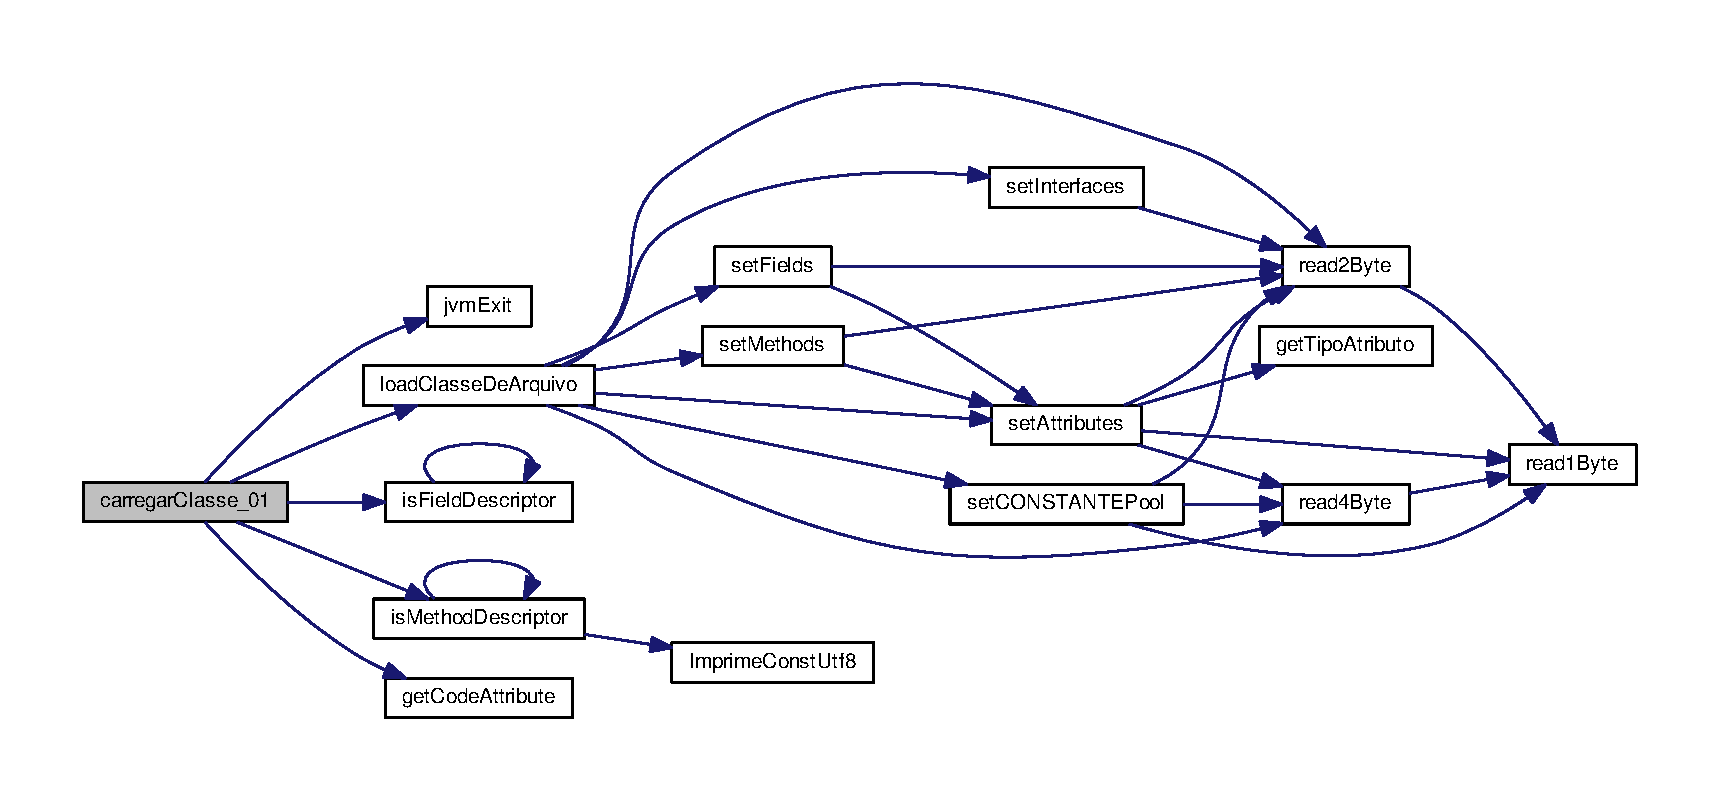
\includegraphics[width=350pt]{core_8h_a7c9daf914ef558b41a9d0b2d617dab86_cgraph}
\end{center}
\end{figure}




Este é o diagrama das funções que utilizam esta função\-:
\nopagebreak
\begin{figure}[H]
\begin{center}
\leavevmode
\includegraphics[width=350pt]{core_8h_a7c9daf914ef558b41a9d0b2d617dab86_icgraph}
\end{center}
\end{figure}


\hypertarget{core_8h_a1c9426d6a17b70527ebee8b467688fa5}{\index{core.\-h@{core.\-h}!class\-Initialization@{class\-Initialization}}
\index{class\-Initialization@{class\-Initialization}!core.h@{core.\-h}}
\subsubsection[{class\-Initialization}]{\setlength{\rightskip}{0pt plus 5cm}void class\-Initialization (
\begin{DoxyParamCaption}
\item[{{\bf D\-A\-D\-O\-S\-\_\-\-C\-L\-A\-S\-S\-E} $\ast$}]{, }
\item[{{\bf J\-V\-M} $\ast$}]{, }
\item[{{\bf T\-H\-R\-E\-A\-D} $\ast$}]{}
\end{DoxyParamCaption}
)}}\label{core_8h_a1c9426d6a17b70527ebee8b467688fa5}


Este é o diagrama das funções que utilizam esta função\-:
\nopagebreak
\begin{figure}[H]
\begin{center}
\leavevmode
\includegraphics[width=350pt]{core_8h_a1c9426d6a17b70527ebee8b467688fa5_icgraph}
\end{center}
\end{figure}


\hypertarget{core_8h_a91b4929cb828eb0548542c7a3decf478}{\index{core.\-h@{core.\-h}!class\-Linking\-Preparation@{class\-Linking\-Preparation}}
\index{class\-Linking\-Preparation@{class\-Linking\-Preparation}!core.h@{core.\-h}}
\subsubsection[{class\-Linking\-Preparation}]{\setlength{\rightskip}{0pt plus 5cm}void class\-Linking\-Preparation (
\begin{DoxyParamCaption}
\item[{{\bf D\-A\-D\-O\-S\-\_\-\-C\-L\-A\-S\-S\-E} $\ast$}]{, }
\item[{{\bf J\-V\-M} $\ast$}]{}
\end{DoxyParamCaption}
)}}\label{core_8h_a91b4929cb828eb0548542c7a3decf478}


Definido na linha 281 do ficheiro cruzeiro.\-c.



Grafo de chamadas desta função\-:\nopagebreak
\begin{figure}[H]
\begin{center}
\leavevmode
\includegraphics[width=286pt]{core_8h_a91b4929cb828eb0548542c7a3decf478_cgraph}
\end{center}
\end{figure}




Este é o diagrama das funções que utilizam esta função\-:\nopagebreak
\begin{figure}[H]
\begin{center}
\leavevmode
\includegraphics[width=350pt]{core_8h_a91b4929cb828eb0548542c7a3decf478_icgraph}
\end{center}
\end{figure}


\hypertarget{core_8h_af99bc13e312e4a07ce2532d2331d2fe3}{\index{core.\-h@{core.\-h}!class\-Linking\-Resolution@{class\-Linking\-Resolution}}
\index{class\-Linking\-Resolution@{class\-Linking\-Resolution}!core.h@{core.\-h}}
\subsubsection[{class\-Linking\-Resolution}]{\setlength{\rightskip}{0pt plus 5cm}void class\-Linking\-Resolution (
\begin{DoxyParamCaption}
\item[{{\bf Classe\-De\-Arquivo} $\ast$}]{, }
\item[{{\bf J\-V\-M} $\ast$}]{}
\end{DoxyParamCaption}
)}}\label{core_8h_af99bc13e312e4a07ce2532d2331d2fe3}
\hypertarget{core_8h_a253fa443bfd7f2b86cee348ce7233035}{\index{core.\-h@{core.\-h}!class\-Linking\-Verification@{class\-Linking\-Verification}}
\index{class\-Linking\-Verification@{class\-Linking\-Verification}!core.h@{core.\-h}}
\subsubsection[{class\-Linking\-Verification}]{\setlength{\rightskip}{0pt plus 5cm}void class\-Linking\-Verification (
\begin{DoxyParamCaption}
\item[{{\bf D\-A\-D\-O\-S\-\_\-\-C\-L\-A\-S\-S\-E} $\ast$}]{, }
\item[{{\bf J\-V\-M} $\ast$}]{}
\end{DoxyParamCaption}
)}}\label{core_8h_a253fa443bfd7f2b86cee348ce7233035}


Definido na linha 250 do ficheiro cruzeiro.\-c.



Grafo de chamadas desta função\-:\nopagebreak
\begin{figure}[H]
\begin{center}
\leavevmode
\includegraphics[width=350pt]{core_8h_a253fa443bfd7f2b86cee348ce7233035_cgraph}
\end{center}
\end{figure}




Este é o diagrama das funções que utilizam esta função\-:\nopagebreak
\begin{figure}[H]
\begin{center}
\leavevmode
\includegraphics[width=350pt]{core_8h_a253fa443bfd7f2b86cee348ce7233035_icgraph}
\end{center}
\end{figure}


\hypertarget{core_8h_a8c96cdaa4bfb0049ed9c2ee068803961}{\index{core.\-h@{core.\-h}!class\-Unloading@{class\-Unloading}}
\index{class\-Unloading@{class\-Unloading}!core.h@{core.\-h}}
\subsubsection[{class\-Unloading}]{\setlength{\rightskip}{0pt plus 5cm}void class\-Unloading (
\begin{DoxyParamCaption}
\item[{{\bf D\-A\-D\-O\-S\-\_\-\-C\-L\-A\-S\-S\-E} $\ast$}]{, }
\item[{{\bf J\-V\-M} $\ast$}]{}
\end{DoxyParamCaption}
)}}\label{core_8h_a8c96cdaa4bfb0049ed9c2ee068803961}
\hypertarget{core_8h_a898cb628ddd2a974d8989a13d9323459}{\index{core.\-h@{core.\-h}!execute\-Method@{execute\-Method}}
\index{execute\-Method@{execute\-Method}!core.h@{core.\-h}}
\subsubsection[{execute\-Method}]{\setlength{\rightskip}{0pt plus 5cm}void execute\-Method (
\begin{DoxyParamCaption}
\item[{char $\ast$}]{, }
\item[{char $\ast$}]{, }
\item[{{\bf D\-A\-D\-O\-S\-\_\-\-C\-L\-A\-S\-S\-E} $\ast$}]{, }
\item[{{\bf J\-V\-M} $\ast$}]{, }
\item[{{\bf T\-H\-R\-E\-A\-D} $\ast$}]{, }
\item[{void $\ast$}]{, }
\item[{uint16\-\_\-t}]{, }
\item[{uint32\-\_\-t $\ast$}]{}
\end{DoxyParamCaption}
)}}\label{core_8h_a898cb628ddd2a974d8989a13d9323459}


Este é o diagrama das funções que utilizam esta função\-:
\nopagebreak
\begin{figure}[H]
\begin{center}
\leavevmode
\includegraphics[width=338pt]{core_8h_a898cb628ddd2a974d8989a13d9323459_icgraph}
\end{center}
\end{figure}


\hypertarget{core_8h_afa9de2a389a6ad80bf97ffa0a5eef402}{\index{core.\-h@{core.\-h}!free\-Arrays@{free\-Arrays}}
\index{free\-Arrays@{free\-Arrays}!core.h@{core.\-h}}
\subsubsection[{free\-Arrays}]{\setlength{\rightskip}{0pt plus 5cm}void free\-Arrays (
\begin{DoxyParamCaption}
\item[{{\bf A\-R\-R\-A\-Y} $\ast$}]{}
\end{DoxyParamCaption}
)}}\label{core_8h_afa9de2a389a6ad80bf97ffa0a5eef402}
\hypertarget{core_8h_ab34a58b2e6a6901430c3c6c025c5c5c6}{\index{core.\-h@{core.\-h}!free\-Class\-Data@{free\-Class\-Data}}
\index{free\-Class\-Data@{free\-Class\-Data}!core.h@{core.\-h}}
\subsubsection[{free\-Class\-Data}]{\setlength{\rightskip}{0pt plus 5cm}void free\-Class\-Data (
\begin{DoxyParamCaption}
\item[{{\bf D\-A\-D\-O\-S\-\_\-\-C\-L\-A\-S\-S\-E} $\ast$}]{}
\end{DoxyParamCaption}
)}}\label{core_8h_ab34a58b2e6a6901430c3c6c025c5c5c6}
\hypertarget{core_8h_abbc22effef4dba84ae83d5e6d1e3da4b}{\index{core.\-h@{core.\-h}!free\-Frame@{free\-Frame}}
\index{free\-Frame@{free\-Frame}!core.h@{core.\-h}}
\subsubsection[{free\-Frame}]{\setlength{\rightskip}{0pt plus 5cm}void free\-Frame (
\begin{DoxyParamCaption}
\item[{{\bf F\-R\-A\-M\-E} $\ast$}]{}
\end{DoxyParamCaption}
)}}\label{core_8h_abbc22effef4dba84ae83d5e6d1e3da4b}


Este é o diagrama das funções que utilizam esta função\-:\nopagebreak
\begin{figure}[H]
\begin{center}
\leavevmode
\includegraphics[width=226pt]{core_8h_abbc22effef4dba84ae83d5e6d1e3da4b_icgraph}
\end{center}
\end{figure}


\hypertarget{core_8h_a4bfc9fc3dd56d8ad9327db10219d2ae3}{\index{core.\-h@{core.\-h}!free\-Heap@{free\-Heap}}
\index{free\-Heap@{free\-Heap}!core.h@{core.\-h}}
\subsubsection[{free\-Heap}]{\setlength{\rightskip}{0pt plus 5cm}void free\-Heap (
\begin{DoxyParamCaption}
\item[{{\bf H\-E\-A\-P\-\_\-\-A\-R\-E\-A} $\ast$}]{}
\end{DoxyParamCaption}
)}}\label{core_8h_a4bfc9fc3dd56d8ad9327db10219d2ae3}
\hypertarget{core_8h_a135eacb54215249d2fb634c920c16d99}{\index{core.\-h@{core.\-h}!free\-Jvm\-Stack@{free\-Jvm\-Stack}}
\index{free\-Jvm\-Stack@{free\-Jvm\-Stack}!core.h@{core.\-h}}
\subsubsection[{free\-Jvm\-Stack}]{\setlength{\rightskip}{0pt plus 5cm}void free\-Jvm\-Stack (
\begin{DoxyParamCaption}
\item[{{\bf F\-R\-A\-M\-E} $\ast$}]{}
\end{DoxyParamCaption}
)}}\label{core_8h_a135eacb54215249d2fb634c920c16d99}
\hypertarget{core_8h_a4074439f529db8ac5c67c1064e0b1b37}{\index{core.\-h@{core.\-h}!free\-Method\-Area@{free\-Method\-Area}}
\index{free\-Method\-Area@{free\-Method\-Area}!core.h@{core.\-h}}
\subsubsection[{free\-Method\-Area}]{\setlength{\rightskip}{0pt plus 5cm}void free\-Method\-Area (
\begin{DoxyParamCaption}
\item[{{\bf D\-A\-D\-O\-S\-\_\-\-C\-L\-A\-S\-S\-E} $\ast$}]{}
\end{DoxyParamCaption}
)}}\label{core_8h_a4074439f529db8ac5c67c1064e0b1b37}
\hypertarget{core_8h_a769094478f2fd98914bfb300f04982f6}{\index{core.\-h@{core.\-h}!free\-Objects@{free\-Objects}}
\index{free\-Objects@{free\-Objects}!core.h@{core.\-h}}
\subsubsection[{free\-Objects}]{\setlength{\rightskip}{0pt plus 5cm}void free\-Objects (
\begin{DoxyParamCaption}
\item[{{\bf O\-B\-J\-E\-C\-T} $\ast$}]{}
\end{DoxyParamCaption}
)}}\label{core_8h_a769094478f2fd98914bfb300f04982f6}
\hypertarget{core_8h_a360c5e8ed32f1b8c1222fe180f02f3cc}{\index{core.\-h@{core.\-h}!free\-Operand\-Stack@{free\-Operand\-Stack}}
\index{free\-Operand\-Stack@{free\-Operand\-Stack}!core.h@{core.\-h}}
\subsubsection[{free\-Operand\-Stack}]{\setlength{\rightskip}{0pt plus 5cm}void free\-Operand\-Stack (
\begin{DoxyParamCaption}
\item[{{\bf F\-R\-A\-M\-E} $\ast$}]{}
\end{DoxyParamCaption}
)}}\label{core_8h_a360c5e8ed32f1b8c1222fe180f02f3cc}
\hypertarget{core_8h_ae038c26bdcbf2be5dca8839cd6c6b5f4}{\index{core.\-h@{core.\-h}!free\-Threads@{free\-Threads}}
\index{free\-Threads@{free\-Threads}!core.h@{core.\-h}}
\subsubsection[{free\-Threads}]{\setlength{\rightskip}{0pt plus 5cm}void free\-Threads (
\begin{DoxyParamCaption}
\item[{{\bf T\-H\-R\-E\-A\-D} $\ast$}]{}
\end{DoxyParamCaption}
)}}\label{core_8h_ae038c26bdcbf2be5dca8839cd6c6b5f4}
\hypertarget{core_8h_ab6c8ef9f9ac6072962115bd3085d4b4b}{\index{core.\-h@{core.\-h}!free\-Variables@{free\-Variables}}
\index{free\-Variables@{free\-Variables}!core.h@{core.\-h}}
\subsubsection[{free\-Variables}]{\setlength{\rightskip}{0pt plus 5cm}void free\-Variables (
\begin{DoxyParamCaption}
\item[{{\bf V\-A\-R\-I\-A\-B\-L\-E} $\ast$}]{}
\end{DoxyParamCaption}
)}}\label{core_8h_ab6c8ef9f9ac6072962115bd3085d4b4b}
\hypertarget{core_8h_a467c17ad6f6b14784f8e861342b1d0e1}{\index{core.\-h@{core.\-h}!get\-Class@{get\-Class}}
\index{get\-Class@{get\-Class}!core.h@{core.\-h}}
\subsubsection[{get\-Class}]{\setlength{\rightskip}{0pt plus 5cm}{\bf D\-A\-D\-O\-S\-\_\-\-C\-L\-A\-S\-S\-E}$\ast$ get\-Class (
\begin{DoxyParamCaption}
\item[{{\bf const\-Pool\-Inf} $\ast$}]{, }
\item[{{\bf J\-V\-M} $\ast$}]{}
\end{DoxyParamCaption}
)}}\label{core_8h_a467c17ad6f6b14784f8e861342b1d0e1}


Este é o diagrama das funções que utilizam esta função\-:\nopagebreak
\begin{figure}[H]
\begin{center}
\leavevmode
\includegraphics[width=246pt]{core_8h_a467c17ad6f6b14784f8e861342b1d0e1_icgraph}
\end{center}
\end{figure}


\hypertarget{core_8h_a4f9e90c40bb4308abdd0c48f6d7086cc}{\index{core.\-h@{core.\-h}!get\-Class\-Name@{get\-Class\-Name}}
\index{get\-Class\-Name@{get\-Class\-Name}!core.h@{core.\-h}}
\subsubsection[{get\-Class\-Name}]{\setlength{\rightskip}{0pt plus 5cm}char$\ast$ get\-Class\-Name (
\begin{DoxyParamCaption}
\item[{{\bf D\-A\-D\-O\-S\-\_\-\-C\-L\-A\-S\-S\-E} $\ast$}]{}
\end{DoxyParamCaption}
)}}\label{core_8h_a4f9e90c40bb4308abdd0c48f6d7086cc}
\hypertarget{core_8h_aa49c64914922c2156b4b03feabf50257}{\index{core.\-h@{core.\-h}!get\-Class\-Variable@{get\-Class\-Variable}}
\index{get\-Class\-Variable@{get\-Class\-Variable}!core.h@{core.\-h}}
\subsubsection[{get\-Class\-Variable}]{\setlength{\rightskip}{0pt plus 5cm}{\bf V\-A\-R\-I\-A\-B\-L\-E}$\ast$ get\-Class\-Variable (
\begin{DoxyParamCaption}
\item[{{\bf const\-Pool\-Inf} $\ast$}]{, }
\item[{{\bf D\-A\-D\-O\-S\-\_\-\-C\-L\-A\-S\-S\-E} $\ast$}]{}
\end{DoxyParamCaption}
)}}\label{core_8h_aa49c64914922c2156b4b03feabf50257}


Este é o diagrama das funções que utilizam esta função\-:\nopagebreak
\begin{figure}[H]
\begin{center}
\leavevmode
\includegraphics[width=278pt]{core_8h_aa49c64914922c2156b4b03feabf50257_icgraph}
\end{center}
\end{figure}


\hypertarget{core_8h_a853d382621b6e22797ee41cc0af6e38f}{\index{core.\-h@{core.\-h}!get\-Code\-Attribute@{get\-Code\-Attribute}}
\index{get\-Code\-Attribute@{get\-Code\-Attribute}!core.h@{core.\-h}}
\subsubsection[{get\-Code\-Attribute}]{\setlength{\rightskip}{0pt plus 5cm}{\bf attribute\-\_\-info}$\ast$ get\-Code\-Attribute (
\begin{DoxyParamCaption}
\item[{{\bf M\-E\-T\-H\-O\-D\-\_\-\-D\-A\-T\-A} $\ast$}]{, }
\item[{{\bf D\-A\-D\-O\-S\-\_\-\-C\-L\-A\-S\-S\-E} $\ast$}]{}
\end{DoxyParamCaption}
)}}\label{core_8h_a853d382621b6e22797ee41cc0af6e38f}


Este é o diagrama das funções que utilizam esta função\-:
\nopagebreak
\begin{figure}[H]
\begin{center}
\leavevmode
\includegraphics[width=350pt]{core_8h_a853d382621b6e22797ee41cc0af6e38f_icgraph}
\end{center}
\end{figure}


\hypertarget{core_8h_a1e9d1e52d8528a1003cd9c699bb87ab9}{\index{core.\-h@{core.\-h}!get\-Instance\-Variable@{get\-Instance\-Variable}}
\index{get\-Instance\-Variable@{get\-Instance\-Variable}!core.h@{core.\-h}}
\subsubsection[{get\-Instance\-Variable}]{\setlength{\rightskip}{0pt plus 5cm}{\bf V\-A\-R\-I\-A\-B\-L\-E}$\ast$ get\-Instance\-Variable (
\begin{DoxyParamCaption}
\item[{{\bf const\-Pool\-Inf} $\ast$}]{, }
\item[{{\bf O\-B\-J\-E\-C\-T} $\ast$}]{}
\end{DoxyParamCaption}
)}}\label{core_8h_a1e9d1e52d8528a1003cd9c699bb87ab9}


Este é o diagrama das funções que utilizam esta função\-:\nopagebreak
\begin{figure}[H]
\begin{center}
\leavevmode
\includegraphics[width=290pt]{core_8h_a1e9d1e52d8528a1003cd9c699bb87ab9_icgraph}
\end{center}
\end{figure}


\hypertarget{core_8h_a2c5411b2b86a128776b99b1310a29bc2}{\index{core.\-h@{core.\-h}!get\-Method@{get\-Method}}
\index{get\-Method@{get\-Method}!core.h@{core.\-h}}
\subsubsection[{get\-Method}]{\setlength{\rightskip}{0pt plus 5cm}{\bf M\-E\-T\-H\-O\-D\-\_\-\-D\-A\-T\-A}$\ast$ get\-Method (
\begin{DoxyParamCaption}
\item[{char $\ast$}]{, }
\item[{char $\ast$}]{, }
\item[{{\bf D\-A\-D\-O\-S\-\_\-\-C\-L\-A\-S\-S\-E} $\ast$}]{, }
\item[{{\bf J\-V\-M} $\ast$}]{}
\end{DoxyParamCaption}
)}}\label{core_8h_a2c5411b2b86a128776b99b1310a29bc2}


Este é o diagrama das funções que utilizam esta função\-:\nopagebreak
\begin{figure}[H]
\begin{center}
\leavevmode
\includegraphics[width=224pt]{core_8h_a2c5411b2b86a128776b99b1310a29bc2_icgraph}
\end{center}
\end{figure}


\hypertarget{core_8h_aaa52a592057a81d501ee49d8d1c81301}{\index{core.\-h@{core.\-h}!get\-Super\-Class@{get\-Super\-Class}}
\index{get\-Super\-Class@{get\-Super\-Class}!core.h@{core.\-h}}
\subsubsection[{get\-Super\-Class}]{\setlength{\rightskip}{0pt plus 5cm}{\bf D\-A\-D\-O\-S\-\_\-\-C\-L\-A\-S\-S\-E}$\ast$ get\-Super\-Class (
\begin{DoxyParamCaption}
\item[{{\bf Classe\-De\-Arquivo} $\ast$}]{, }
\item[{{\bf J\-V\-M} $\ast$}]{}
\end{DoxyParamCaption}
)}}\label{core_8h_aaa52a592057a81d501ee49d8d1c81301}


Este é o diagrama das funções que utilizam esta função\-:
\nopagebreak
\begin{figure}[H]
\begin{center}
\leavevmode
\includegraphics[width=350pt]{core_8h_aaa52a592057a81d501ee49d8d1c81301_icgraph}
\end{center}
\end{figure}


\hypertarget{core_8h_aa2f1283af56df2749e5702e0b569c5d7}{\index{core.\-h@{core.\-h}!iniciar\-\_\-jvm@{iniciar\-\_\-jvm}}
\index{iniciar\-\_\-jvm@{iniciar\-\_\-jvm}!core.h@{core.\-h}}
\subsubsection[{iniciar\-\_\-jvm}]{\setlength{\rightskip}{0pt plus 5cm}void iniciar\-\_\-jvm (
\begin{DoxyParamCaption}
\item[{char $\ast$}]{, }
\item[{int}]{, }
\item[{char $\ast$$\ast$}]{}
\end{DoxyParamCaption}
)}}\label{core_8h_aa2f1283af56df2749e5702e0b569c5d7}


Definido na linha 10 do ficheiro cruzeiro.\-c.



Grafo de chamadas desta função\-:\nopagebreak
\begin{figure}[H]
\begin{center}
\leavevmode
\includegraphics[width=350pt]{core_8h_aa2f1283af56df2749e5702e0b569c5d7_cgraph}
\end{center}
\end{figure}




Este é o diagrama das funções que utilizam esta função\-:\nopagebreak
\begin{figure}[H]
\begin{center}
\leavevmode
\includegraphics[width=218pt]{core_8h_aa2f1283af56df2749e5702e0b569c5d7_icgraph}
\end{center}
\end{figure}


\hypertarget{core_8h_a18b8702b615b635f6b52e95c60ed73b1}{\index{core.\-h@{core.\-h}!is\-Super\-Class@{is\-Super\-Class}}
\index{is\-Super\-Class@{is\-Super\-Class}!core.h@{core.\-h}}
\subsubsection[{is\-Super\-Class}]{\setlength{\rightskip}{0pt plus 5cm}bool is\-Super\-Class (
\begin{DoxyParamCaption}
\item[{{\bf D\-A\-D\-O\-S\-\_\-\-C\-L\-A\-S\-S\-E} $\ast$}]{, }
\item[{{\bf D\-A\-D\-O\-S\-\_\-\-C\-L\-A\-S\-S\-E} $\ast$}]{, }
\item[{{\bf J\-V\-M} $\ast$}]{}
\end{DoxyParamCaption}
)}}\label{core_8h_a18b8702b615b635f6b52e95c60ed73b1}


Este é o diagrama das funções que utilizam esta função\-:\nopagebreak
\begin{figure}[H]
\begin{center}
\leavevmode
\includegraphics[width=262pt]{core_8h_a18b8702b615b635f6b52e95c60ed73b1_icgraph}
\end{center}
\end{figure}


\hypertarget{core_8h_a65309fe2f949999b73fa78000ffec3c4}{\index{core.\-h@{core.\-h}!jvm\-Exit@{jvm\-Exit}}
\index{jvm\-Exit@{jvm\-Exit}!core.h@{core.\-h}}
\subsubsection[{jvm\-Exit}]{\setlength{\rightskip}{0pt plus 5cm}void jvm\-Exit (
\begin{DoxyParamCaption}
\item[{{\bf J\-V\-M} $\ast$}]{}
\end{DoxyParamCaption}
)}}\label{core_8h_a65309fe2f949999b73fa78000ffec3c4}


Este é o diagrama das funções que utilizam esta função\-:
\nopagebreak
\begin{figure}[H]
\begin{center}
\leavevmode
\includegraphics[width=350pt]{core_8h_a65309fe2f949999b73fa78000ffec3c4_icgraph}
\end{center}
\end{figure}


\hypertarget{core_8h_a92753a3e4a70b1837b498b2821b1c478}{\index{core.\-h@{core.\-h}!ligador\-De\-Classe@{ligador\-De\-Classe}}
\index{ligador\-De\-Classe@{ligador\-De\-Classe}!core.h@{core.\-h}}
\subsubsection[{ligador\-De\-Classe}]{\setlength{\rightskip}{0pt plus 5cm}void ligador\-De\-Classe (
\begin{DoxyParamCaption}
\item[{{\bf D\-A\-D\-O\-S\-\_\-\-C\-L\-A\-S\-S\-E} $\ast$}]{, }
\item[{{\bf J\-V\-M} $\ast$}]{}
\end{DoxyParamCaption}
)}}\label{core_8h_a92753a3e4a70b1837b498b2821b1c478}


Definido na linha 243 do ficheiro cruzeiro.\-c.



Grafo de chamadas desta função\-:\nopagebreak
\begin{figure}[H]
\begin{center}
\leavevmode
\includegraphics[width=350pt]{core_8h_a92753a3e4a70b1837b498b2821b1c478_cgraph}
\end{center}
\end{figure}




Este é o diagrama das funções que utilizam esta função\-:
\nopagebreak
\begin{figure}[H]
\begin{center}
\leavevmode
\includegraphics[width=350pt]{core_8h_a92753a3e4a70b1837b498b2821b1c478_icgraph}
\end{center}
\end{figure}


\hypertarget{core_8h_a01ea050bc682333139b2b64e89008893}{\index{core.\-h@{core.\-h}!pop\-Operand@{pop\-Operand}}
\index{pop\-Operand@{pop\-Operand}!core.h@{core.\-h}}
\subsubsection[{pop\-Operand}]{\setlength{\rightskip}{0pt plus 5cm}uint32\-\_\-t pop\-Operand (
\begin{DoxyParamCaption}
\item[{{\bf F\-R\-A\-M\-E} $\ast$}]{}
\end{DoxyParamCaption}
)}}\label{core_8h_a01ea050bc682333139b2b64e89008893}


Este é o diagrama das funções que utilizam esta função\-:\nopagebreak
\begin{figure}[H]
\begin{center}
\leavevmode
\includegraphics[height=550pt]{core_8h_a01ea050bc682333139b2b64e89008893_icgraph}
\end{center}
\end{figure}


\hypertarget{core_8h_ada292ff1b4724c764f4cc6ff992cce06}{\index{core.\-h@{core.\-h}!push\-Operand@{push\-Operand}}
\index{push\-Operand@{push\-Operand}!core.h@{core.\-h}}
\subsubsection[{push\-Operand}]{\setlength{\rightskip}{0pt plus 5cm}void push\-Operand (
\begin{DoxyParamCaption}
\item[{uint32\-\_\-t}]{, }
\item[{{\bf F\-R\-A\-M\-E} $\ast$}]{}
\end{DoxyParamCaption}
)}}\label{core_8h_ada292ff1b4724c764f4cc6ff992cce06}


Este é o diagrama das funções que utilizam esta função\-:\nopagebreak
\begin{figure}[H]
\begin{center}
\leavevmode
\includegraphics[height=550pt]{core_8h_ada292ff1b4724c764f4cc6ff992cce06_icgraph}
\end{center}
\end{figure}



\hypertarget{cruzeiro_8c}{\section{Referência ao ficheiro cruzeiro.\-c}
\label{cruzeiro_8c}\index{cruzeiro.\-c@{cruzeiro.\-c}}
}
{\ttfamily \#include \char`\"{}interpreter.\-h\char`\"{}}\\*
Diagrama de dependências de inclusão para cruzeiro.\-c\-:
\nopagebreak
\begin{figure}[H]
\begin{center}
\leavevmode
\includegraphics[width=350pt]{cruzeiro_8c__incl}
\end{center}
\end{figure}
\subsection*{Funções}
\begin{DoxyCompactItemize}
\item 
void \hyperlink{cruzeiro_8c_aee16aa11ac6dc26f08b24ee6b446bc50}{iniciar\-\_\-jvm} (char $\ast$nome\-Do\-Arquivo\-De\-Classe, int num\-\_\-args, char $\ast$$\ast$args)
\item 
void \hyperlink{cruzeiro_8c_a044f22337572729fe6a256eac0ff4820}{carregar\-Classe\-\_\-01} (char $\ast$nome\-Do\-Arquivo\-De\-Classe, \hyperlink{struct_d_a_d_o_s___c_l_a_s_s_e}{D\-A\-D\-O\-S\-\_\-\-C\-L\-A\-S\-S\-E} $\ast$$\ast$cd, \hyperlink{struct_d_a_d_o_s___c_l_a_s_s_e}{D\-A\-D\-O\-S\-\_\-\-C\-L\-A\-S\-S\-E} $\ast$carregador\-Classe, \hyperlink{core_8h_a98bdb4b2c8aa49ba6bcd37df96469137}{J\-V\-M} $\ast$\hyperlink{structjvm}{jvm})
\item 
void \hyperlink{cruzeiro_8c_aa6c77c38ce0e50b4e897fa2470abfca7}{ligador\-De\-Classe} (\hyperlink{struct_d_a_d_o_s___c_l_a_s_s_e}{D\-A\-D\-O\-S\-\_\-\-C\-L\-A\-S\-S\-E} $\ast$cd, \hyperlink{core_8h_a98bdb4b2c8aa49ba6bcd37df96469137}{J\-V\-M} $\ast$\hyperlink{structjvm}{jvm})
\item 
void \hyperlink{cruzeiro_8c_a63268a53fa4c29f6663370e343c7a610}{class\-Linking\-Verification} (\hyperlink{struct_d_a_d_o_s___c_l_a_s_s_e}{D\-A\-D\-O\-S\-\_\-\-C\-L\-A\-S\-S\-E} $\ast$cd, \hyperlink{core_8h_a98bdb4b2c8aa49ba6bcd37df96469137}{J\-V\-M} $\ast$\hyperlink{structjvm}{jvm})
\item 
void \hyperlink{cruzeiro_8c_a5a186301f1f3a10e62e93674c07c2fcc}{class\-Linking\-Preparation} (\hyperlink{struct_d_a_d_o_s___c_l_a_s_s_e}{D\-A\-D\-O\-S\-\_\-\-C\-L\-A\-S\-S\-E} $\ast$cd, \hyperlink{core_8h_a98bdb4b2c8aa49ba6bcd37df96469137}{J\-V\-M} $\ast$\hyperlink{structjvm}{jvm})
\end{DoxyCompactItemize}


\subsection{Documentação das funções}
\hypertarget{cruzeiro_8c_a044f22337572729fe6a256eac0ff4820}{\index{cruzeiro.\-c@{cruzeiro.\-c}!carregar\-Classe\-\_\-01@{carregar\-Classe\-\_\-01}}
\index{carregar\-Classe\-\_\-01@{carregar\-Classe\-\_\-01}!cruzeiro.c@{cruzeiro.\-c}}
\subsubsection[{carregar\-Classe\-\_\-01}]{\setlength{\rightskip}{0pt plus 5cm}void carregar\-Classe\-\_\-01 (
\begin{DoxyParamCaption}
\item[{char $\ast$}]{nome\-Do\-Arquivo\-De\-Classe, }
\item[{{\bf D\-A\-D\-O\-S\-\_\-\-C\-L\-A\-S\-S\-E} $\ast$$\ast$}]{cd, }
\item[{{\bf D\-A\-D\-O\-S\-\_\-\-C\-L\-A\-S\-S\-E} $\ast$}]{carregador\-Classe, }
\item[{{\bf J\-V\-M} $\ast$}]{jvm}
\end{DoxyParamCaption}
)}}\label{cruzeiro_8c_a044f22337572729fe6a256eac0ff4820}


Definido na linha 113 do ficheiro cruzeiro.\-c.



Grafo de chamadas desta função\-:\nopagebreak
\begin{figure}[H]
\begin{center}
\leavevmode
\includegraphics[width=350pt]{cruzeiro_8c_a044f22337572729fe6a256eac0ff4820_cgraph}
\end{center}
\end{figure}




Este é o diagrama das funções que utilizam esta função\-:
\nopagebreak
\begin{figure}[H]
\begin{center}
\leavevmode
\includegraphics[width=350pt]{cruzeiro_8c_a044f22337572729fe6a256eac0ff4820_icgraph}
\end{center}
\end{figure}


\hypertarget{cruzeiro_8c_a5a186301f1f3a10e62e93674c07c2fcc}{\index{cruzeiro.\-c@{cruzeiro.\-c}!class\-Linking\-Preparation@{class\-Linking\-Preparation}}
\index{class\-Linking\-Preparation@{class\-Linking\-Preparation}!cruzeiro.c@{cruzeiro.\-c}}
\subsubsection[{class\-Linking\-Preparation}]{\setlength{\rightskip}{0pt plus 5cm}void class\-Linking\-Preparation (
\begin{DoxyParamCaption}
\item[{{\bf D\-A\-D\-O\-S\-\_\-\-C\-L\-A\-S\-S\-E} $\ast$}]{cd, }
\item[{{\bf J\-V\-M} $\ast$}]{jvm}
\end{DoxyParamCaption}
)}}\label{cruzeiro_8c_a5a186301f1f3a10e62e93674c07c2fcc}


Definido na linha 281 do ficheiro cruzeiro.\-c.



Grafo de chamadas desta função\-:\nopagebreak
\begin{figure}[H]
\begin{center}
\leavevmode
\includegraphics[width=286pt]{cruzeiro_8c_a5a186301f1f3a10e62e93674c07c2fcc_cgraph}
\end{center}
\end{figure}




Este é o diagrama das funções que utilizam esta função\-:
\nopagebreak
\begin{figure}[H]
\begin{center}
\leavevmode
\includegraphics[width=350pt]{cruzeiro_8c_a5a186301f1f3a10e62e93674c07c2fcc_icgraph}
\end{center}
\end{figure}


\hypertarget{cruzeiro_8c_a63268a53fa4c29f6663370e343c7a610}{\index{cruzeiro.\-c@{cruzeiro.\-c}!class\-Linking\-Verification@{class\-Linking\-Verification}}
\index{class\-Linking\-Verification@{class\-Linking\-Verification}!cruzeiro.c@{cruzeiro.\-c}}
\subsubsection[{class\-Linking\-Verification}]{\setlength{\rightskip}{0pt plus 5cm}void class\-Linking\-Verification (
\begin{DoxyParamCaption}
\item[{{\bf D\-A\-D\-O\-S\-\_\-\-C\-L\-A\-S\-S\-E} $\ast$}]{cd, }
\item[{{\bf J\-V\-M} $\ast$}]{jvm}
\end{DoxyParamCaption}
)}}\label{cruzeiro_8c_a63268a53fa4c29f6663370e343c7a610}


Definido na linha 250 do ficheiro cruzeiro.\-c.



Grafo de chamadas desta função\-:\nopagebreak
\begin{figure}[H]
\begin{center}
\leavevmode
\includegraphics[width=350pt]{cruzeiro_8c_a63268a53fa4c29f6663370e343c7a610_cgraph}
\end{center}
\end{figure}




Este é o diagrama das funções que utilizam esta função\-:
\nopagebreak
\begin{figure}[H]
\begin{center}
\leavevmode
\includegraphics[width=350pt]{cruzeiro_8c_a63268a53fa4c29f6663370e343c7a610_icgraph}
\end{center}
\end{figure}


\hypertarget{cruzeiro_8c_aee16aa11ac6dc26f08b24ee6b446bc50}{\index{cruzeiro.\-c@{cruzeiro.\-c}!iniciar\-\_\-jvm@{iniciar\-\_\-jvm}}
\index{iniciar\-\_\-jvm@{iniciar\-\_\-jvm}!cruzeiro.c@{cruzeiro.\-c}}
\subsubsection[{iniciar\-\_\-jvm}]{\setlength{\rightskip}{0pt plus 5cm}void iniciar\-\_\-jvm (
\begin{DoxyParamCaption}
\item[{char $\ast$}]{nome\-Do\-Arquivo\-De\-Classe, }
\item[{int}]{num\-\_\-args, }
\item[{char $\ast$$\ast$}]{args}
\end{DoxyParamCaption}
)}}\label{cruzeiro_8c_aee16aa11ac6dc26f08b24ee6b446bc50}


Definido na linha 10 do ficheiro cruzeiro.\-c.



Grafo de chamadas desta função\-:\nopagebreak
\begin{figure}[H]
\begin{center}
\leavevmode
\includegraphics[width=350pt]{cruzeiro_8c_aee16aa11ac6dc26f08b24ee6b446bc50_cgraph}
\end{center}
\end{figure}




Este é o diagrama das funções que utilizam esta função\-:\nopagebreak
\begin{figure}[H]
\begin{center}
\leavevmode
\includegraphics[width=218pt]{cruzeiro_8c_aee16aa11ac6dc26f08b24ee6b446bc50_icgraph}
\end{center}
\end{figure}


\hypertarget{cruzeiro_8c_aa6c77c38ce0e50b4e897fa2470abfca7}{\index{cruzeiro.\-c@{cruzeiro.\-c}!ligador\-De\-Classe@{ligador\-De\-Classe}}
\index{ligador\-De\-Classe@{ligador\-De\-Classe}!cruzeiro.c@{cruzeiro.\-c}}
\subsubsection[{ligador\-De\-Classe}]{\setlength{\rightskip}{0pt plus 5cm}void ligador\-De\-Classe (
\begin{DoxyParamCaption}
\item[{{\bf D\-A\-D\-O\-S\-\_\-\-C\-L\-A\-S\-S\-E} $\ast$}]{cd, }
\item[{{\bf J\-V\-M} $\ast$}]{jvm}
\end{DoxyParamCaption}
)}}\label{cruzeiro_8c_aa6c77c38ce0e50b4e897fa2470abfca7}


Definido na linha 243 do ficheiro cruzeiro.\-c.



Grafo de chamadas desta função\-:\nopagebreak
\begin{figure}[H]
\begin{center}
\leavevmode
\includegraphics[width=350pt]{cruzeiro_8c_aa6c77c38ce0e50b4e897fa2470abfca7_cgraph}
\end{center}
\end{figure}




Este é o diagrama das funções que utilizam esta função\-:
\nopagebreak
\begin{figure}[H]
\begin{center}
\leavevmode
\includegraphics[width=350pt]{cruzeiro_8c_aa6c77c38ce0e50b4e897fa2470abfca7_icgraph}
\end{center}
\end{figure}



\hypertarget{interpreter_8c}{\section{Referência ao ficheiro interpreter.\-c}
\label{interpreter_8c}\index{interpreter.\-c@{interpreter.\-c}}
}
{\ttfamily \#include \char`\"{}interpreter.\-h\char`\"{}}\\*
{\ttfamily \#include \char`\"{}opcode.\-h\char`\"{}}\\*
{\ttfamily \#include $<$errno.\-h$>$}\\*
Diagrama de dependências de inclusão para interpreter.\-c\-:
\nopagebreak
\begin{figure}[H]
\begin{center}
\leavevmode
\includegraphics[width=350pt]{interpreter_8c__incl}
\end{center}
\end{figure}
\subsection*{Macros}
\begin{DoxyCompactItemize}
\item 
\#define \hyperlink{interpreter_8c_aaa1ac5caef84256eaeb39594e58e096f}{M\-A\-X\-\_\-\-I\-N\-T}~2147483647
\item 
\#define \hyperlink{interpreter_8c_a91a4a7c68f549b5f31dbced70ae07ee6}{M\-I\-N\-\_\-\-I\-N\-T}~–2147483648
\end{DoxyCompactItemize}
\subsection*{Funções}
\begin{DoxyCompactItemize}
\item 
void \hyperlink{interpreter_8c_a321f0344c7fbe872cb02c015f4a38a99}{interpreter} (\hyperlink{core_8h_af2592f49e52b0675aaca5850571f3999}{M\-E\-T\-H\-O\-D\-\_\-\-D\-A\-T\-A} $\ast$method, \hyperlink{core_8h_ad43b7ffe97b146f9dce917ae2a0fd181}{T\-H\-R\-E\-A\-D} $\ast$\hyperlink{structthread}{thread}, \hyperlink{core_8h_a98bdb4b2c8aa49ba6bcd37df96469137}{J\-V\-M} $\ast$\hyperlink{structjvm}{jvm})
\item 
void \hyperlink{interpreter_8c_a1479000369abdedd8c4867548645d407}{nop\-\_\-} (\hyperlink{core_8h_af2592f49e52b0675aaca5850571f3999}{M\-E\-T\-H\-O\-D\-\_\-\-D\-A\-T\-A} $\ast$method, \hyperlink{core_8h_ad43b7ffe97b146f9dce917ae2a0fd181}{T\-H\-R\-E\-A\-D} $\ast$\hyperlink{structthread}{thread}, \hyperlink{core_8h_a98bdb4b2c8aa49ba6bcd37df96469137}{J\-V\-M} $\ast$\hyperlink{structjvm}{jvm})
\item 
void \hyperlink{interpreter_8c_afda8502640018aeb806c2e63a67d0664}{Tconst} (\hyperlink{core_8h_af2592f49e52b0675aaca5850571f3999}{M\-E\-T\-H\-O\-D\-\_\-\-D\-A\-T\-A} $\ast$method, \hyperlink{core_8h_ad43b7ffe97b146f9dce917ae2a0fd181}{T\-H\-R\-E\-A\-D} $\ast$\hyperlink{structthread}{thread}, \hyperlink{core_8h_a98bdb4b2c8aa49ba6bcd37df96469137}{J\-V\-M} $\ast$\hyperlink{structjvm}{jvm})
\item 
void \hyperlink{interpreter_8c_addfdf844ff8e7f06e669a75e7cbede75}{Tipush} (\hyperlink{core_8h_af2592f49e52b0675aaca5850571f3999}{M\-E\-T\-H\-O\-D\-\_\-\-D\-A\-T\-A} $\ast$method, \hyperlink{core_8h_ad43b7ffe97b146f9dce917ae2a0fd181}{T\-H\-R\-E\-A\-D} $\ast$\hyperlink{structthread}{thread}, \hyperlink{core_8h_a98bdb4b2c8aa49ba6bcd37df96469137}{J\-V\-M} $\ast$\hyperlink{structjvm}{jvm})
\item 
void \hyperlink{interpreter_8c_ab8ad4ed015e92554ba35534108c734cb}{ldc\-\_\-} (\hyperlink{core_8h_af2592f49e52b0675aaca5850571f3999}{M\-E\-T\-H\-O\-D\-\_\-\-D\-A\-T\-A} $\ast$method, \hyperlink{core_8h_ad43b7ffe97b146f9dce917ae2a0fd181}{T\-H\-R\-E\-A\-D} $\ast$\hyperlink{structthread}{thread}, \hyperlink{core_8h_a98bdb4b2c8aa49ba6bcd37df96469137}{J\-V\-M} $\ast$\hyperlink{structjvm}{jvm})
\item 
void \hyperlink{interpreter_8c_a7dbacd0b8f567e0e0d0fc7da5c9d2011}{Tload} (\hyperlink{core_8h_af2592f49e52b0675aaca5850571f3999}{M\-E\-T\-H\-O\-D\-\_\-\-D\-A\-T\-A} $\ast$method, \hyperlink{core_8h_ad43b7ffe97b146f9dce917ae2a0fd181}{T\-H\-R\-E\-A\-D} $\ast$\hyperlink{structthread}{thread}, \hyperlink{core_8h_a98bdb4b2c8aa49ba6bcd37df96469137}{J\-V\-M} $\ast$\hyperlink{structjvm}{jvm})
\item 
void \hyperlink{interpreter_8c_ab61e478627a533c4574e0d2f9bcaf120}{Taload} (\hyperlink{core_8h_af2592f49e52b0675aaca5850571f3999}{M\-E\-T\-H\-O\-D\-\_\-\-D\-A\-T\-A} $\ast$method, \hyperlink{core_8h_ad43b7ffe97b146f9dce917ae2a0fd181}{T\-H\-R\-E\-A\-D} $\ast$\hyperlink{structthread}{thread}, \hyperlink{core_8h_a98bdb4b2c8aa49ba6bcd37df96469137}{J\-V\-M} $\ast$\hyperlink{structjvm}{jvm})
\item 
void \hyperlink{interpreter_8c_ad5aeffe10805e0e1cf18eaedaf193279}{Tstore} (\hyperlink{core_8h_af2592f49e52b0675aaca5850571f3999}{M\-E\-T\-H\-O\-D\-\_\-\-D\-A\-T\-A} $\ast$method, \hyperlink{core_8h_ad43b7ffe97b146f9dce917ae2a0fd181}{T\-H\-R\-E\-A\-D} $\ast$\hyperlink{structthread}{thread}, \hyperlink{core_8h_a98bdb4b2c8aa49ba6bcd37df96469137}{J\-V\-M} $\ast$\hyperlink{structjvm}{jvm})
\item 
void \hyperlink{interpreter_8c_ac7cc8f18408416f3e391e3e9565ab0f0}{Tastore} (\hyperlink{core_8h_af2592f49e52b0675aaca5850571f3999}{M\-E\-T\-H\-O\-D\-\_\-\-D\-A\-T\-A} $\ast$method, \hyperlink{core_8h_ad43b7ffe97b146f9dce917ae2a0fd181}{T\-H\-R\-E\-A\-D} $\ast$\hyperlink{structthread}{thread}, \hyperlink{core_8h_a98bdb4b2c8aa49ba6bcd37df96469137}{J\-V\-M} $\ast$\hyperlink{structjvm}{jvm})
\item 
void \hyperlink{interpreter_8c_ac9f409a905c3c48cd6921bcb144b88ac}{handle\-Stack} (\hyperlink{core_8h_af2592f49e52b0675aaca5850571f3999}{M\-E\-T\-H\-O\-D\-\_\-\-D\-A\-T\-A} $\ast$method, \hyperlink{core_8h_ad43b7ffe97b146f9dce917ae2a0fd181}{T\-H\-R\-E\-A\-D} $\ast$\hyperlink{structthread}{thread}, \hyperlink{core_8h_a98bdb4b2c8aa49ba6bcd37df96469137}{J\-V\-M} $\ast$\hyperlink{structjvm}{jvm})
\item 
void \hyperlink{interpreter_8c_a228415cfd84d5942f890a6198e62ec5d}{Tadd} (\hyperlink{core_8h_af2592f49e52b0675aaca5850571f3999}{M\-E\-T\-H\-O\-D\-\_\-\-D\-A\-T\-A} $\ast$method, \hyperlink{core_8h_ad43b7ffe97b146f9dce917ae2a0fd181}{T\-H\-R\-E\-A\-D} $\ast$\hyperlink{structthread}{thread}, \hyperlink{core_8h_a98bdb4b2c8aa49ba6bcd37df96469137}{J\-V\-M} $\ast$\hyperlink{structjvm}{jvm})
\item 
void \hyperlink{interpreter_8c_a079c9f1558666a24b332615608be90fb}{Tsub} (\hyperlink{core_8h_af2592f49e52b0675aaca5850571f3999}{M\-E\-T\-H\-O\-D\-\_\-\-D\-A\-T\-A} $\ast$method, \hyperlink{core_8h_ad43b7ffe97b146f9dce917ae2a0fd181}{T\-H\-R\-E\-A\-D} $\ast$\hyperlink{structthread}{thread}, \hyperlink{core_8h_a98bdb4b2c8aa49ba6bcd37df96469137}{J\-V\-M} $\ast$\hyperlink{structjvm}{jvm})
\item 
void \hyperlink{interpreter_8c_aab90abdb67ec6d414874e91dc0850e2b}{Tmul} (\hyperlink{core_8h_af2592f49e52b0675aaca5850571f3999}{M\-E\-T\-H\-O\-D\-\_\-\-D\-A\-T\-A} $\ast$method, \hyperlink{core_8h_ad43b7ffe97b146f9dce917ae2a0fd181}{T\-H\-R\-E\-A\-D} $\ast$\hyperlink{structthread}{thread}, \hyperlink{core_8h_a98bdb4b2c8aa49ba6bcd37df96469137}{J\-V\-M} $\ast$\hyperlink{structjvm}{jvm})
\item 
void \hyperlink{interpreter_8c_adf4d2d942e551e69c15298698379ccf4}{Tdiv} (\hyperlink{core_8h_af2592f49e52b0675aaca5850571f3999}{M\-E\-T\-H\-O\-D\-\_\-\-D\-A\-T\-A} $\ast$method, \hyperlink{core_8h_ad43b7ffe97b146f9dce917ae2a0fd181}{T\-H\-R\-E\-A\-D} $\ast$\hyperlink{structthread}{thread}, \hyperlink{core_8h_a98bdb4b2c8aa49ba6bcd37df96469137}{J\-V\-M} $\ast$\hyperlink{structjvm}{jvm})
\item 
void \hyperlink{interpreter_8c_a56e323c2c15653fb2f5f251a536fbea7}{Trem} (\hyperlink{core_8h_af2592f49e52b0675aaca5850571f3999}{M\-E\-T\-H\-O\-D\-\_\-\-D\-A\-T\-A} $\ast$method, \hyperlink{core_8h_ad43b7ffe97b146f9dce917ae2a0fd181}{T\-H\-R\-E\-A\-D} $\ast$\hyperlink{structthread}{thread}, \hyperlink{core_8h_a98bdb4b2c8aa49ba6bcd37df96469137}{J\-V\-M} $\ast$\hyperlink{structjvm}{jvm})
\item 
void \hyperlink{interpreter_8c_ac83f45cc4a0f3191dd34f6ac5f9c0ffc}{Tneg} (\hyperlink{core_8h_af2592f49e52b0675aaca5850571f3999}{M\-E\-T\-H\-O\-D\-\_\-\-D\-A\-T\-A} $\ast$method, \hyperlink{core_8h_ad43b7ffe97b146f9dce917ae2a0fd181}{T\-H\-R\-E\-A\-D} $\ast$\hyperlink{structthread}{thread}, \hyperlink{core_8h_a98bdb4b2c8aa49ba6bcd37df96469137}{J\-V\-M} $\ast$\hyperlink{structjvm}{jvm})
\item 
void \hyperlink{interpreter_8c_afa9436a1637151b02587dc8d6b2e5380}{Tshl} (\hyperlink{core_8h_af2592f49e52b0675aaca5850571f3999}{M\-E\-T\-H\-O\-D\-\_\-\-D\-A\-T\-A} $\ast$method, \hyperlink{core_8h_ad43b7ffe97b146f9dce917ae2a0fd181}{T\-H\-R\-E\-A\-D} $\ast$\hyperlink{structthread}{thread}, \hyperlink{core_8h_a98bdb4b2c8aa49ba6bcd37df96469137}{J\-V\-M} $\ast$\hyperlink{structjvm}{jvm})
\item 
void \hyperlink{interpreter_8c_a5cc0ed983a4fe8c7639dd618e7e4ca04}{Tshr} (\hyperlink{core_8h_af2592f49e52b0675aaca5850571f3999}{M\-E\-T\-H\-O\-D\-\_\-\-D\-A\-T\-A} $\ast$method, \hyperlink{core_8h_ad43b7ffe97b146f9dce917ae2a0fd181}{T\-H\-R\-E\-A\-D} $\ast$\hyperlink{structthread}{thread}, \hyperlink{core_8h_a98bdb4b2c8aa49ba6bcd37df96469137}{J\-V\-M} $\ast$\hyperlink{structjvm}{jvm})
\item 
void \hyperlink{interpreter_8c_a33c94f8aceef240fb7077377fceca521}{Tushr} (\hyperlink{core_8h_af2592f49e52b0675aaca5850571f3999}{M\-E\-T\-H\-O\-D\-\_\-\-D\-A\-T\-A} $\ast$method, \hyperlink{core_8h_ad43b7ffe97b146f9dce917ae2a0fd181}{T\-H\-R\-E\-A\-D} $\ast$\hyperlink{structthread}{thread}, \hyperlink{core_8h_a98bdb4b2c8aa49ba6bcd37df96469137}{J\-V\-M} $\ast$\hyperlink{structjvm}{jvm})
\item 
void \hyperlink{interpreter_8c_aa1d57458e6177d9bd258c6516201cedf}{Tand} (\hyperlink{core_8h_af2592f49e52b0675aaca5850571f3999}{M\-E\-T\-H\-O\-D\-\_\-\-D\-A\-T\-A} $\ast$method, \hyperlink{core_8h_ad43b7ffe97b146f9dce917ae2a0fd181}{T\-H\-R\-E\-A\-D} $\ast$\hyperlink{structthread}{thread}, \hyperlink{core_8h_a98bdb4b2c8aa49ba6bcd37df96469137}{J\-V\-M} $\ast$\hyperlink{structjvm}{jvm})
\item 
void \hyperlink{interpreter_8c_ac453160594afd71686861153623a097e}{Tor} (\hyperlink{core_8h_af2592f49e52b0675aaca5850571f3999}{M\-E\-T\-H\-O\-D\-\_\-\-D\-A\-T\-A} $\ast$method, \hyperlink{core_8h_ad43b7ffe97b146f9dce917ae2a0fd181}{T\-H\-R\-E\-A\-D} $\ast$\hyperlink{structthread}{thread}, \hyperlink{core_8h_a98bdb4b2c8aa49ba6bcd37df96469137}{J\-V\-M} $\ast$\hyperlink{structjvm}{jvm})
\item 
void \hyperlink{interpreter_8c_af56099fd754edf06c996085f2162253b}{Txor} (\hyperlink{core_8h_af2592f49e52b0675aaca5850571f3999}{M\-E\-T\-H\-O\-D\-\_\-\-D\-A\-T\-A} $\ast$method, \hyperlink{core_8h_ad43b7ffe97b146f9dce917ae2a0fd181}{T\-H\-R\-E\-A\-D} $\ast$\hyperlink{structthread}{thread}, \hyperlink{core_8h_a98bdb4b2c8aa49ba6bcd37df96469137}{J\-V\-M} $\ast$\hyperlink{structjvm}{jvm})
\item 
void \hyperlink{interpreter_8c_af938654f06c247d579b463274fc59ecf}{Tinc} (\hyperlink{core_8h_af2592f49e52b0675aaca5850571f3999}{M\-E\-T\-H\-O\-D\-\_\-\-D\-A\-T\-A} $\ast$method, \hyperlink{core_8h_ad43b7ffe97b146f9dce917ae2a0fd181}{T\-H\-R\-E\-A\-D} $\ast$\hyperlink{structthread}{thread}, \hyperlink{core_8h_a98bdb4b2c8aa49ba6bcd37df96469137}{J\-V\-M} $\ast$\hyperlink{structjvm}{jvm})
\item 
void \hyperlink{interpreter_8c_ae40aac245cc9a047bceb2758778523c0}{i2\-T} (\hyperlink{core_8h_af2592f49e52b0675aaca5850571f3999}{M\-E\-T\-H\-O\-D\-\_\-\-D\-A\-T\-A} $\ast$method, \hyperlink{core_8h_ad43b7ffe97b146f9dce917ae2a0fd181}{T\-H\-R\-E\-A\-D} $\ast$\hyperlink{structthread}{thread}, \hyperlink{core_8h_a98bdb4b2c8aa49ba6bcd37df96469137}{J\-V\-M} $\ast$\hyperlink{structjvm}{jvm})
\item 
void \hyperlink{interpreter_8c_a739135ead120fb6081986e2cedf2dc9f}{l2\-T} (\hyperlink{core_8h_af2592f49e52b0675aaca5850571f3999}{M\-E\-T\-H\-O\-D\-\_\-\-D\-A\-T\-A} $\ast$method, \hyperlink{core_8h_ad43b7ffe97b146f9dce917ae2a0fd181}{T\-H\-R\-E\-A\-D} $\ast$\hyperlink{structthread}{thread}, \hyperlink{core_8h_a98bdb4b2c8aa49ba6bcd37df96469137}{J\-V\-M} $\ast$\hyperlink{structjvm}{jvm})
\item 
void \hyperlink{interpreter_8c_ade1c69d439aa79742d9144d6eb5616c5}{f2\-T} (\hyperlink{core_8h_af2592f49e52b0675aaca5850571f3999}{M\-E\-T\-H\-O\-D\-\_\-\-D\-A\-T\-A} $\ast$method, \hyperlink{core_8h_ad43b7ffe97b146f9dce917ae2a0fd181}{T\-H\-R\-E\-A\-D} $\ast$\hyperlink{structthread}{thread}, \hyperlink{core_8h_a98bdb4b2c8aa49ba6bcd37df96469137}{J\-V\-M} $\ast$\hyperlink{structjvm}{jvm})
\item 
void \hyperlink{interpreter_8c_a560b57e699e82fbfeb88e79fdd79be31}{d2\-T} (\hyperlink{core_8h_af2592f49e52b0675aaca5850571f3999}{M\-E\-T\-H\-O\-D\-\_\-\-D\-A\-T\-A} $\ast$method, \hyperlink{core_8h_ad43b7ffe97b146f9dce917ae2a0fd181}{T\-H\-R\-E\-A\-D} $\ast$\hyperlink{structthread}{thread}, \hyperlink{core_8h_a98bdb4b2c8aa49ba6bcd37df96469137}{J\-V\-M} $\ast$\hyperlink{structjvm}{jvm})
\item 
void \hyperlink{interpreter_8c_a882f006c29b07b71e2a61ab3173bc4f4}{Tcmp} (\hyperlink{core_8h_af2592f49e52b0675aaca5850571f3999}{M\-E\-T\-H\-O\-D\-\_\-\-D\-A\-T\-A} $\ast$method, \hyperlink{core_8h_ad43b7ffe97b146f9dce917ae2a0fd181}{T\-H\-R\-E\-A\-D} $\ast$\hyperlink{structthread}{thread}, \hyperlink{core_8h_a98bdb4b2c8aa49ba6bcd37df96469137}{J\-V\-M} $\ast$\hyperlink{structjvm}{jvm})
\item 
void \hyperlink{interpreter_8c_abed429497737ff29ed6b0715edbde549}{Tcmp\-O\-P} (\hyperlink{core_8h_af2592f49e52b0675aaca5850571f3999}{M\-E\-T\-H\-O\-D\-\_\-\-D\-A\-T\-A} $\ast$method, \hyperlink{core_8h_ad43b7ffe97b146f9dce917ae2a0fd181}{T\-H\-R\-E\-A\-D} $\ast$\hyperlink{structthread}{thread}, \hyperlink{core_8h_a98bdb4b2c8aa49ba6bcd37df96469137}{J\-V\-M} $\ast$\hyperlink{structjvm}{jvm})
\item 
void \hyperlink{interpreter_8c_a7027a19e214f5a48abb0f13a5971cc2a}{if\-O\-P} (\hyperlink{core_8h_af2592f49e52b0675aaca5850571f3999}{M\-E\-T\-H\-O\-D\-\_\-\-D\-A\-T\-A} $\ast$method, \hyperlink{core_8h_ad43b7ffe97b146f9dce917ae2a0fd181}{T\-H\-R\-E\-A\-D} $\ast$\hyperlink{structthread}{thread}, \hyperlink{core_8h_a98bdb4b2c8aa49ba6bcd37df96469137}{J\-V\-M} $\ast$\hyperlink{structjvm}{jvm})
\item 
void \hyperlink{interpreter_8c_ad198896294076b4ebd7146536d130e2c}{if\-\_\-icm\-O\-P} (\hyperlink{core_8h_af2592f49e52b0675aaca5850571f3999}{M\-E\-T\-H\-O\-D\-\_\-\-D\-A\-T\-A} $\ast$method, \hyperlink{core_8h_ad43b7ffe97b146f9dce917ae2a0fd181}{T\-H\-R\-E\-A\-D} $\ast$\hyperlink{structthread}{thread}, \hyperlink{core_8h_a98bdb4b2c8aa49ba6bcd37df96469137}{J\-V\-M} $\ast$\hyperlink{structjvm}{jvm})
\item 
void \hyperlink{interpreter_8c_a4e570063469ee691624f4ad94fa1b543}{if\-\_\-acm\-O\-P} (\hyperlink{core_8h_af2592f49e52b0675aaca5850571f3999}{M\-E\-T\-H\-O\-D\-\_\-\-D\-A\-T\-A} $\ast$method, \hyperlink{core_8h_ad43b7ffe97b146f9dce917ae2a0fd181}{T\-H\-R\-E\-A\-D} $\ast$\hyperlink{structthread}{thread}, \hyperlink{core_8h_a98bdb4b2c8aa49ba6bcd37df96469137}{J\-V\-M} $\ast$\hyperlink{structjvm}{jvm})
\item 
void \hyperlink{interpreter_8c_a10d49ce1dfe761db660383e2f3a3d5b2}{jump} (\hyperlink{core_8h_af2592f49e52b0675aaca5850571f3999}{M\-E\-T\-H\-O\-D\-\_\-\-D\-A\-T\-A} $\ast$method, \hyperlink{core_8h_ad43b7ffe97b146f9dce917ae2a0fd181}{T\-H\-R\-E\-A\-D} $\ast$\hyperlink{structthread}{thread}, \hyperlink{core_8h_a98bdb4b2c8aa49ba6bcd37df96469137}{J\-V\-M} $\ast$\hyperlink{structjvm}{jvm})
\item 
void \hyperlink{interpreter_8c_ad6df0e2f95b53ac2fb8fec8328f1a190}{switch\-\_\-} (\hyperlink{core_8h_af2592f49e52b0675aaca5850571f3999}{M\-E\-T\-H\-O\-D\-\_\-\-D\-A\-T\-A} $\ast$method, \hyperlink{core_8h_ad43b7ffe97b146f9dce917ae2a0fd181}{T\-H\-R\-E\-A\-D} $\ast$\hyperlink{structthread}{thread}, \hyperlink{core_8h_a98bdb4b2c8aa49ba6bcd37df96469137}{J\-V\-M} $\ast$\hyperlink{structjvm}{jvm})
\item 
void \hyperlink{interpreter_8c_a36fdbabed5a911fa8b0cb4568c582d46}{Treturn} (\hyperlink{core_8h_af2592f49e52b0675aaca5850571f3999}{M\-E\-T\-H\-O\-D\-\_\-\-D\-A\-T\-A} $\ast$method, \hyperlink{core_8h_ad43b7ffe97b146f9dce917ae2a0fd181}{T\-H\-R\-E\-A\-D} $\ast$\hyperlink{structthread}{thread}, \hyperlink{core_8h_a98bdb4b2c8aa49ba6bcd37df96469137}{J\-V\-M} $\ast$\hyperlink{structjvm}{jvm})
\item 
void \hyperlink{interpreter_8c_a3a69cbad0d9de40b20b8bfcd8b8e1894}{access\-Field} (\hyperlink{core_8h_af2592f49e52b0675aaca5850571f3999}{M\-E\-T\-H\-O\-D\-\_\-\-D\-A\-T\-A} $\ast$method, \hyperlink{core_8h_ad43b7ffe97b146f9dce917ae2a0fd181}{T\-H\-R\-E\-A\-D} $\ast$\hyperlink{structthread}{thread}, \hyperlink{core_8h_a98bdb4b2c8aa49ba6bcd37df96469137}{J\-V\-M} $\ast$\hyperlink{structjvm}{jvm})
\item 
void \hyperlink{interpreter_8c_a86d2c1a67286ba0d59aea4dc12c4bff9}{invoke} (\hyperlink{core_8h_af2592f49e52b0675aaca5850571f3999}{M\-E\-T\-H\-O\-D\-\_\-\-D\-A\-T\-A} $\ast$method, \hyperlink{core_8h_ad43b7ffe97b146f9dce917ae2a0fd181}{T\-H\-R\-E\-A\-D} $\ast$\hyperlink{structthread}{thread}, \hyperlink{core_8h_a98bdb4b2c8aa49ba6bcd37df96469137}{J\-V\-M} $\ast$\hyperlink{structjvm}{jvm})
\item 
void \hyperlink{interpreter_8c_a087a4ba00043fe2d831ccf04b183a0b5}{handle\-Object} (\hyperlink{core_8h_af2592f49e52b0675aaca5850571f3999}{M\-E\-T\-H\-O\-D\-\_\-\-D\-A\-T\-A} $\ast$method, \hyperlink{core_8h_ad43b7ffe97b146f9dce917ae2a0fd181}{T\-H\-R\-E\-A\-D} $\ast$\hyperlink{structthread}{thread}, \hyperlink{core_8h_a98bdb4b2c8aa49ba6bcd37df96469137}{J\-V\-M} $\ast$\hyperlink{structjvm}{jvm})
\item 
void \hyperlink{interpreter_8c_a1d0e06d16d097e40de348c6815dab9d4}{create\-Multi\-Array} (\hyperlink{core_8h_a9c07c3330f66f4018e49ee90e58f0f39}{A\-R\-R\-A\-Y} $\ast$arrayref, int32\-\_\-t $\ast$count\-\_\-values, uint8\-\_\-t i, uint8\-\_\-t dimensions, \hyperlink{core_8h_a98bdb4b2c8aa49ba6bcd37df96469137}{J\-V\-M} $\ast$\hyperlink{structjvm}{jvm})
\item 
void \hyperlink{interpreter_8c_ad5554bce4b64fbd044a02aa01e49d901}{athrow\-\_\-} (\hyperlink{core_8h_af2592f49e52b0675aaca5850571f3999}{M\-E\-T\-H\-O\-D\-\_\-\-D\-A\-T\-A} $\ast$method, \hyperlink{core_8h_ad43b7ffe97b146f9dce917ae2a0fd181}{T\-H\-R\-E\-A\-D} $\ast$\hyperlink{structthread}{thread}, \hyperlink{core_8h_a98bdb4b2c8aa49ba6bcd37df96469137}{J\-V\-M} $\ast$\hyperlink{structjvm}{jvm})
\item 
void \hyperlink{interpreter_8c_a7402e9c860e8f0bbd146841c2f20e895}{properties} (\hyperlink{core_8h_af2592f49e52b0675aaca5850571f3999}{M\-E\-T\-H\-O\-D\-\_\-\-D\-A\-T\-A} $\ast$method, \hyperlink{core_8h_ad43b7ffe97b146f9dce917ae2a0fd181}{T\-H\-R\-E\-A\-D} $\ast$\hyperlink{structthread}{thread}, \hyperlink{core_8h_a98bdb4b2c8aa49ba6bcd37df96469137}{J\-V\-M} $\ast$\hyperlink{structjvm}{jvm})
\item 
void \hyperlink{interpreter_8c_a65bf7946d0bafb400e3ca90101925725}{monitor} (\hyperlink{core_8h_af2592f49e52b0675aaca5850571f3999}{M\-E\-T\-H\-O\-D\-\_\-\-D\-A\-T\-A} $\ast$method, \hyperlink{core_8h_ad43b7ffe97b146f9dce917ae2a0fd181}{T\-H\-R\-E\-A\-D} $\ast$\hyperlink{structthread}{thread}, \hyperlink{core_8h_a98bdb4b2c8aa49ba6bcd37df96469137}{J\-V\-M} $\ast$\hyperlink{structjvm}{jvm})
\item 
void \hyperlink{interpreter_8c_a94f443e0efca453296685ddc82ff1358}{wide\-\_\-} (\hyperlink{core_8h_af2592f49e52b0675aaca5850571f3999}{M\-E\-T\-H\-O\-D\-\_\-\-D\-A\-T\-A} $\ast$method, \hyperlink{core_8h_ad43b7ffe97b146f9dce917ae2a0fd181}{T\-H\-R\-E\-A\-D} $\ast$\hyperlink{structthread}{thread}, \hyperlink{core_8h_a98bdb4b2c8aa49ba6bcd37df96469137}{J\-V\-M} $\ast$\hyperlink{structjvm}{jvm})
\item 
void \hyperlink{interpreter_8c_a1b7d99078d946b21ec1c5c9634787920}{if\-Null} (\hyperlink{core_8h_af2592f49e52b0675aaca5850571f3999}{M\-E\-T\-H\-O\-D\-\_\-\-D\-A\-T\-A} $\ast$method, \hyperlink{core_8h_ad43b7ffe97b146f9dce917ae2a0fd181}{T\-H\-R\-E\-A\-D} $\ast$\hyperlink{structthread}{thread}, \hyperlink{core_8h_a98bdb4b2c8aa49ba6bcd37df96469137}{J\-V\-M} $\ast$\hyperlink{structjvm}{jvm})
\item 
void \hyperlink{interpreter_8c_ae92a4faa052510290febb645cb54c952}{widejump} (\hyperlink{core_8h_af2592f49e52b0675aaca5850571f3999}{M\-E\-T\-H\-O\-D\-\_\-\-D\-A\-T\-A} $\ast$method, \hyperlink{core_8h_ad43b7ffe97b146f9dce917ae2a0fd181}{T\-H\-R\-E\-A\-D} $\ast$\hyperlink{structthread}{thread}, \hyperlink{core_8h_a98bdb4b2c8aa49ba6bcd37df96469137}{J\-V\-M} $\ast$\hyperlink{structjvm}{jvm})
\item 
void \hyperlink{interpreter_8c_a0eb26886183ccc0cd23bb38f36915c79}{breakpoint\-\_\-} (\hyperlink{core_8h_af2592f49e52b0675aaca5850571f3999}{M\-E\-T\-H\-O\-D\-\_\-\-D\-A\-T\-A} $\ast$method, \hyperlink{core_8h_ad43b7ffe97b146f9dce917ae2a0fd181}{T\-H\-R\-E\-A\-D} $\ast$\hyperlink{structthread}{thread}, \hyperlink{core_8h_a98bdb4b2c8aa49ba6bcd37df96469137}{J\-V\-M} $\ast$\hyperlink{structjvm}{jvm})
\item 
void \hyperlink{interpreter_8c_aea85e27c58a18677d890ad102432aca4}{non\-Defined} (\hyperlink{core_8h_af2592f49e52b0675aaca5850571f3999}{M\-E\-T\-H\-O\-D\-\_\-\-D\-A\-T\-A} $\ast$method, \hyperlink{core_8h_ad43b7ffe97b146f9dce917ae2a0fd181}{T\-H\-R\-E\-A\-D} $\ast$\hyperlink{structthread}{thread}, \hyperlink{core_8h_a98bdb4b2c8aa49ba6bcd37df96469137}{J\-V\-M} $\ast$\hyperlink{structjvm}{jvm})
\item 
void \hyperlink{interpreter_8c_ae56e7a3ef2420b64091b115700a24c10}{impdep} (\hyperlink{core_8h_af2592f49e52b0675aaca5850571f3999}{M\-E\-T\-H\-O\-D\-\_\-\-D\-A\-T\-A} $\ast$method, \hyperlink{core_8h_ad43b7ffe97b146f9dce917ae2a0fd181}{T\-H\-R\-E\-A\-D} $\ast$\hyperlink{structthread}{thread}, \hyperlink{core_8h_a98bdb4b2c8aa49ba6bcd37df96469137}{J\-V\-M} $\ast$\hyperlink{structjvm}{jvm})
\end{DoxyCompactItemize}
\subsection*{Variáveis}
\begin{DoxyCompactItemize}
\item 
char $\ast$ \hyperlink{interpreter_8c_ab085c5e8fbd11f44f0580cca27621d6e}{opcodes\-J\-V\-M} \mbox{[}$\,$\mbox{]}
\item 
int \hyperlink{interpreter_8c_aeaa46a8f05fe44a7db1b8140ca7a3239}{is\-Wide} = 0
\item 
\hyperlink{interpreter_8h_a8861e8ff3f8d80c5805372aed9c2b6ab}{I\-N\-S\-T\-R\-U\-C\-T\-I\-O\-N} \hyperlink{interpreter_8c_a92e41b446c5961ac28375c13970abcd4}{func} \mbox{[}$\,$\mbox{]}
\end{DoxyCompactItemize}


\subsection{Documentação das macros}
\hypertarget{interpreter_8c_aaa1ac5caef84256eaeb39594e58e096f}{\index{interpreter.\-c@{interpreter.\-c}!M\-A\-X\-\_\-\-I\-N\-T@{M\-A\-X\-\_\-\-I\-N\-T}}
\index{M\-A\-X\-\_\-\-I\-N\-T@{M\-A\-X\-\_\-\-I\-N\-T}!interpreter.c@{interpreter.\-c}}
\subsubsection[{M\-A\-X\-\_\-\-I\-N\-T}]{\setlength{\rightskip}{0pt plus 5cm}\#define M\-A\-X\-\_\-\-I\-N\-T~2147483647}}\label{interpreter_8c_aaa1ac5caef84256eaeb39594e58e096f}


Definido na linha 14 do ficheiro interpreter.\-c.

\hypertarget{interpreter_8c_a91a4a7c68f549b5f31dbced70ae07ee6}{\index{interpreter.\-c@{interpreter.\-c}!M\-I\-N\-\_\-\-I\-N\-T@{M\-I\-N\-\_\-\-I\-N\-T}}
\index{M\-I\-N\-\_\-\-I\-N\-T@{M\-I\-N\-\_\-\-I\-N\-T}!interpreter.c@{interpreter.\-c}}
\subsubsection[{M\-I\-N\-\_\-\-I\-N\-T}]{\setlength{\rightskip}{0pt plus 5cm}\#define M\-I\-N\-\_\-\-I\-N\-T~–2147483648}}\label{interpreter_8c_a91a4a7c68f549b5f31dbced70ae07ee6}


Definido na linha 15 do ficheiro interpreter.\-c.



\subsection{Documentação das funções}
\hypertarget{interpreter_8c_a3a69cbad0d9de40b20b8bfcd8b8e1894}{\index{interpreter.\-c@{interpreter.\-c}!access\-Field@{access\-Field}}
\index{access\-Field@{access\-Field}!interpreter.c@{interpreter.\-c}}
\subsubsection[{access\-Field}]{\setlength{\rightskip}{0pt plus 5cm}void access\-Field (
\begin{DoxyParamCaption}
\item[{{\bf M\-E\-T\-H\-O\-D\-\_\-\-D\-A\-T\-A} $\ast$}]{method, }
\item[{{\bf T\-H\-R\-E\-A\-D} $\ast$}]{thread, }
\item[{{\bf J\-V\-M} $\ast$}]{jvm}
\end{DoxyParamCaption}
)}}\label{interpreter_8c_a3a69cbad0d9de40b20b8bfcd8b8e1894}


Definido na linha 2373 do ficheiro interpreter.\-c.



Grafo de chamadas desta função\-:
\nopagebreak
\begin{figure}[H]
\begin{center}
\leavevmode
\includegraphics[width=350pt]{interpreter_8c_a3a69cbad0d9de40b20b8bfcd8b8e1894_cgraph}
\end{center}
\end{figure}


\hypertarget{interpreter_8c_ad5554bce4b64fbd044a02aa01e49d901}{\index{interpreter.\-c@{interpreter.\-c}!athrow\-\_\-@{athrow\-\_\-}}
\index{athrow\-\_\-@{athrow\-\_\-}!interpreter.c@{interpreter.\-c}}
\subsubsection[{athrow\-\_\-}]{\setlength{\rightskip}{0pt plus 5cm}void athrow\-\_\- (
\begin{DoxyParamCaption}
\item[{{\bf M\-E\-T\-H\-O\-D\-\_\-\-D\-A\-T\-A} $\ast$}]{method, }
\item[{{\bf T\-H\-R\-E\-A\-D} $\ast$}]{thread, }
\item[{{\bf J\-V\-M} $\ast$}]{jvm}
\end{DoxyParamCaption}
)}}\label{interpreter_8c_ad5554bce4b64fbd044a02aa01e49d901}


Definido na linha 4049 do ficheiro interpreter.\-c.

\hypertarget{interpreter_8c_a0eb26886183ccc0cd23bb38f36915c79}{\index{interpreter.\-c@{interpreter.\-c}!breakpoint\-\_\-@{breakpoint\-\_\-}}
\index{breakpoint\-\_\-@{breakpoint\-\_\-}!interpreter.c@{interpreter.\-c}}
\subsubsection[{breakpoint\-\_\-}]{\setlength{\rightskip}{0pt plus 5cm}void breakpoint\-\_\- (
\begin{DoxyParamCaption}
\item[{{\bf M\-E\-T\-H\-O\-D\-\_\-\-D\-A\-T\-A} $\ast$}]{method, }
\item[{{\bf T\-H\-R\-E\-A\-D} $\ast$}]{thread, }
\item[{{\bf J\-V\-M} $\ast$}]{jvm}
\end{DoxyParamCaption}
)}}\label{interpreter_8c_a0eb26886183ccc0cd23bb38f36915c79}


Definido na linha 4154 do ficheiro interpreter.\-c.

\hypertarget{interpreter_8c_a1d0e06d16d097e40de348c6815dab9d4}{\index{interpreter.\-c@{interpreter.\-c}!create\-Multi\-Array@{create\-Multi\-Array}}
\index{create\-Multi\-Array@{create\-Multi\-Array}!interpreter.c@{interpreter.\-c}}
\subsubsection[{create\-Multi\-Array}]{\setlength{\rightskip}{0pt plus 5cm}void create\-Multi\-Array (
\begin{DoxyParamCaption}
\item[{{\bf A\-R\-R\-A\-Y} $\ast$}]{arrayref, }
\item[{int32\-\_\-t $\ast$}]{count\-\_\-values, }
\item[{uint8\-\_\-t}]{i, }
\item[{uint8\-\_\-t}]{dimensions, }
\item[{{\bf J\-V\-M} $\ast$}]{jvm}
\end{DoxyParamCaption}
)}}\label{interpreter_8c_a1d0e06d16d097e40de348c6815dab9d4}


Definido na linha 4030 do ficheiro interpreter.\-c.



Grafo de chamadas desta função\-:\nopagebreak
\begin{figure}[H]
\begin{center}
\leavevmode
\includegraphics[width=168pt]{interpreter_8c_a1d0e06d16d097e40de348c6815dab9d4_cgraph}
\end{center}
\end{figure}




Este é o diagrama das funções que utilizam esta função\-:\nopagebreak
\begin{figure}[H]
\begin{center}
\leavevmode
\includegraphics[width=350pt]{interpreter_8c_a1d0e06d16d097e40de348c6815dab9d4_icgraph}
\end{center}
\end{figure}


\hypertarget{interpreter_8c_a560b57e699e82fbfeb88e79fdd79be31}{\index{interpreter.\-c@{interpreter.\-c}!d2\-T@{d2\-T}}
\index{d2\-T@{d2\-T}!interpreter.c@{interpreter.\-c}}
\subsubsection[{d2\-T}]{\setlength{\rightskip}{0pt plus 5cm}void d2\-T (
\begin{DoxyParamCaption}
\item[{{\bf M\-E\-T\-H\-O\-D\-\_\-\-D\-A\-T\-A} $\ast$}]{method, }
\item[{{\bf T\-H\-R\-E\-A\-D} $\ast$}]{thread, }
\item[{{\bf J\-V\-M} $\ast$}]{jvm}
\end{DoxyParamCaption}
)}}\label{interpreter_8c_a560b57e699e82fbfeb88e79fdd79be31}


Definido na linha 1825 do ficheiro interpreter.\-c.



Grafo de chamadas desta função\-:\nopagebreak
\begin{figure}[H]
\begin{center}
\leavevmode
\includegraphics[width=224pt]{interpreter_8c_a560b57e699e82fbfeb88e79fdd79be31_cgraph}
\end{center}
\end{figure}


\hypertarget{interpreter_8c_ade1c69d439aa79742d9144d6eb5616c5}{\index{interpreter.\-c@{interpreter.\-c}!f2\-T@{f2\-T}}
\index{f2\-T@{f2\-T}!interpreter.c@{interpreter.\-c}}
\subsubsection[{f2\-T}]{\setlength{\rightskip}{0pt plus 5cm}void f2\-T (
\begin{DoxyParamCaption}
\item[{{\bf M\-E\-T\-H\-O\-D\-\_\-\-D\-A\-T\-A} $\ast$}]{method, }
\item[{{\bf T\-H\-R\-E\-A\-D} $\ast$}]{thread, }
\item[{{\bf J\-V\-M} $\ast$}]{jvm}
\end{DoxyParamCaption}
)}}\label{interpreter_8c_ade1c69d439aa79742d9144d6eb5616c5}


Definido na linha 1766 do ficheiro interpreter.\-c.



Grafo de chamadas desta função\-:\nopagebreak
\begin{figure}[H]
\begin{center}
\leavevmode
\includegraphics[width=222pt]{interpreter_8c_ade1c69d439aa79742d9144d6eb5616c5_cgraph}
\end{center}
\end{figure}


\hypertarget{interpreter_8c_a087a4ba00043fe2d831ccf04b183a0b5}{\index{interpreter.\-c@{interpreter.\-c}!handle\-Object@{handle\-Object}}
\index{handle\-Object@{handle\-Object}!interpreter.c@{interpreter.\-c}}
\subsubsection[{handle\-Object}]{\setlength{\rightskip}{0pt plus 5cm}void handle\-Object (
\begin{DoxyParamCaption}
\item[{{\bf M\-E\-T\-H\-O\-D\-\_\-\-D\-A\-T\-A} $\ast$}]{method, }
\item[{{\bf T\-H\-R\-E\-A\-D} $\ast$}]{thread, }
\item[{{\bf J\-V\-M} $\ast$}]{jvm}
\end{DoxyParamCaption}
)}}\label{interpreter_8c_a087a4ba00043fe2d831ccf04b183a0b5}


Definido na linha 3598 do ficheiro interpreter.\-c.



Grafo de chamadas desta função\-:
\nopagebreak
\begin{figure}[H]
\begin{center}
\leavevmode
\includegraphics[width=350pt]{interpreter_8c_a087a4ba00043fe2d831ccf04b183a0b5_cgraph}
\end{center}
\end{figure}


\hypertarget{interpreter_8c_ac9f409a905c3c48cd6921bcb144b88ac}{\index{interpreter.\-c@{interpreter.\-c}!handle\-Stack@{handle\-Stack}}
\index{handle\-Stack@{handle\-Stack}!interpreter.c@{interpreter.\-c}}
\subsubsection[{handle\-Stack}]{\setlength{\rightskip}{0pt plus 5cm}void handle\-Stack (
\begin{DoxyParamCaption}
\item[{{\bf M\-E\-T\-H\-O\-D\-\_\-\-D\-A\-T\-A} $\ast$}]{method, }
\item[{{\bf T\-H\-R\-E\-A\-D} $\ast$}]{thread, }
\item[{{\bf J\-V\-M} $\ast$}]{jvm}
\end{DoxyParamCaption}
)}}\label{interpreter_8c_ac9f409a905c3c48cd6921bcb144b88ac}


Definido na linha 632 do ficheiro interpreter.\-c.



Grafo de chamadas desta função\-:\nopagebreak
\begin{figure}[H]
\begin{center}
\leavevmode
\includegraphics[width=262pt]{interpreter_8c_ac9f409a905c3c48cd6921bcb144b88ac_cgraph}
\end{center}
\end{figure}


\hypertarget{interpreter_8c_ae40aac245cc9a047bceb2758778523c0}{\index{interpreter.\-c@{interpreter.\-c}!i2\-T@{i2\-T}}
\index{i2\-T@{i2\-T}!interpreter.c@{interpreter.\-c}}
\subsubsection[{i2\-T}]{\setlength{\rightskip}{0pt plus 5cm}void i2\-T (
\begin{DoxyParamCaption}
\item[{{\bf M\-E\-T\-H\-O\-D\-\_\-\-D\-A\-T\-A} $\ast$}]{method, }
\item[{{\bf T\-H\-R\-E\-A\-D} $\ast$}]{thread, }
\item[{{\bf J\-V\-M} $\ast$}]{jvm}
\end{DoxyParamCaption}
)}}\label{interpreter_8c_ae40aac245cc9a047bceb2758778523c0}


Definido na linha 1614 do ficheiro interpreter.\-c.



Grafo de chamadas desta função\-:\nopagebreak
\begin{figure}[H]
\begin{center}
\leavevmode
\includegraphics[width=220pt]{interpreter_8c_ae40aac245cc9a047bceb2758778523c0_cgraph}
\end{center}
\end{figure}


\hypertarget{interpreter_8c_a4e570063469ee691624f4ad94fa1b543}{\index{interpreter.\-c@{interpreter.\-c}!if\-\_\-acm\-O\-P@{if\-\_\-acm\-O\-P}}
\index{if\-\_\-acm\-O\-P@{if\-\_\-acm\-O\-P}!interpreter.c@{interpreter.\-c}}
\subsubsection[{if\-\_\-acm\-O\-P}]{\setlength{\rightskip}{0pt plus 5cm}void if\-\_\-acm\-O\-P (
\begin{DoxyParamCaption}
\item[{{\bf M\-E\-T\-H\-O\-D\-\_\-\-D\-A\-T\-A} $\ast$}]{method, }
\item[{{\bf T\-H\-R\-E\-A\-D} $\ast$}]{thread, }
\item[{{\bf J\-V\-M} $\ast$}]{jvm}
\end{DoxyParamCaption}
)}}\label{interpreter_8c_a4e570063469ee691624f4ad94fa1b543}


Definido na linha 2133 do ficheiro interpreter.\-c.



Grafo de chamadas desta função\-:\nopagebreak
\begin{figure}[H]
\begin{center}
\leavevmode
\includegraphics[width=246pt]{interpreter_8c_a4e570063469ee691624f4ad94fa1b543_cgraph}
\end{center}
\end{figure}


\hypertarget{interpreter_8c_ad198896294076b4ebd7146536d130e2c}{\index{interpreter.\-c@{interpreter.\-c}!if\-\_\-icm\-O\-P@{if\-\_\-icm\-O\-P}}
\index{if\-\_\-icm\-O\-P@{if\-\_\-icm\-O\-P}!interpreter.c@{interpreter.\-c}}
\subsubsection[{if\-\_\-icm\-O\-P}]{\setlength{\rightskip}{0pt plus 5cm}void if\-\_\-icm\-O\-P (
\begin{DoxyParamCaption}
\item[{{\bf M\-E\-T\-H\-O\-D\-\_\-\-D\-A\-T\-A} $\ast$}]{method, }
\item[{{\bf T\-H\-R\-E\-A\-D} $\ast$}]{thread, }
\item[{{\bf J\-V\-M} $\ast$}]{jvm}
\end{DoxyParamCaption}
)}}\label{interpreter_8c_ad198896294076b4ebd7146536d130e2c}


Definido na linha 2067 do ficheiro interpreter.\-c.



Grafo de chamadas desta função\-:\nopagebreak
\begin{figure}[H]
\begin{center}
\leavevmode
\includegraphics[width=244pt]{interpreter_8c_ad198896294076b4ebd7146536d130e2c_cgraph}
\end{center}
\end{figure}


\hypertarget{interpreter_8c_a1b7d99078d946b21ec1c5c9634787920}{\index{interpreter.\-c@{interpreter.\-c}!if\-Null@{if\-Null}}
\index{if\-Null@{if\-Null}!interpreter.c@{interpreter.\-c}}
\subsubsection[{if\-Null}]{\setlength{\rightskip}{0pt plus 5cm}void if\-Null (
\begin{DoxyParamCaption}
\item[{{\bf M\-E\-T\-H\-O\-D\-\_\-\-D\-A\-T\-A} $\ast$}]{method, }
\item[{{\bf T\-H\-R\-E\-A\-D} $\ast$}]{thread, }
\item[{{\bf J\-V\-M} $\ast$}]{jvm}
\end{DoxyParamCaption}
)}}\label{interpreter_8c_a1b7d99078d946b21ec1c5c9634787920}


Definido na linha 4103 do ficheiro interpreter.\-c.



Grafo de chamadas desta função\-:\nopagebreak
\begin{figure}[H]
\begin{center}
\leavevmode
\includegraphics[width=226pt]{interpreter_8c_a1b7d99078d946b21ec1c5c9634787920_cgraph}
\end{center}
\end{figure}


\hypertarget{interpreter_8c_a7027a19e214f5a48abb0f13a5971cc2a}{\index{interpreter.\-c@{interpreter.\-c}!if\-O\-P@{if\-O\-P}}
\index{if\-O\-P@{if\-O\-P}!interpreter.c@{interpreter.\-c}}
\subsubsection[{if\-O\-P}]{\setlength{\rightskip}{0pt plus 5cm}void if\-O\-P (
\begin{DoxyParamCaption}
\item[{{\bf M\-E\-T\-H\-O\-D\-\_\-\-D\-A\-T\-A} $\ast$}]{method, }
\item[{{\bf T\-H\-R\-E\-A\-D} $\ast$}]{thread, }
\item[{{\bf J\-V\-M} $\ast$}]{jvm}
\end{DoxyParamCaption}
)}}\label{interpreter_8c_a7027a19e214f5a48abb0f13a5971cc2a}


Definido na linha 2001 do ficheiro interpreter.\-c.



Grafo de chamadas desta função\-:\nopagebreak
\begin{figure}[H]
\begin{center}
\leavevmode
\includegraphics[width=222pt]{interpreter_8c_a7027a19e214f5a48abb0f13a5971cc2a_cgraph}
\end{center}
\end{figure}


\hypertarget{interpreter_8c_ae56e7a3ef2420b64091b115700a24c10}{\index{interpreter.\-c@{interpreter.\-c}!impdep@{impdep}}
\index{impdep@{impdep}!interpreter.c@{interpreter.\-c}}
\subsubsection[{impdep}]{\setlength{\rightskip}{0pt plus 5cm}void impdep (
\begin{DoxyParamCaption}
\item[{{\bf M\-E\-T\-H\-O\-D\-\_\-\-D\-A\-T\-A} $\ast$}]{method, }
\item[{{\bf T\-H\-R\-E\-A\-D} $\ast$}]{thread, }
\item[{{\bf J\-V\-M} $\ast$}]{jvm}
\end{DoxyParamCaption}
)}}\label{interpreter_8c_ae56e7a3ef2420b64091b115700a24c10}


Definido na linha 4168 do ficheiro interpreter.\-c.

\hypertarget{interpreter_8c_a321f0344c7fbe872cb02c015f4a38a99}{\index{interpreter.\-c@{interpreter.\-c}!interpreter@{interpreter}}
\index{interpreter@{interpreter}!interpreter.c@{interpreter.\-c}}
\subsubsection[{interpreter}]{\setlength{\rightskip}{0pt plus 5cm}void interpreter (
\begin{DoxyParamCaption}
\item[{{\bf M\-E\-T\-H\-O\-D\-\_\-\-D\-A\-T\-A} $\ast$}]{method, }
\item[{{\bf T\-H\-R\-E\-A\-D} $\ast$}]{thread, }
\item[{{\bf J\-V\-M} $\ast$}]{jvm}
\end{DoxyParamCaption}
)}}\label{interpreter_8c_a321f0344c7fbe872cb02c015f4a38a99}


Definido na linha 27 do ficheiro interpreter.\-c.

\hypertarget{interpreter_8c_a86d2c1a67286ba0d59aea4dc12c4bff9}{\index{interpreter.\-c@{interpreter.\-c}!invoke@{invoke}}
\index{invoke@{invoke}!interpreter.c@{interpreter.\-c}}
\subsubsection[{invoke}]{\setlength{\rightskip}{0pt plus 5cm}void invoke (
\begin{DoxyParamCaption}
\item[{{\bf M\-E\-T\-H\-O\-D\-\_\-\-D\-A\-T\-A} $\ast$}]{method, }
\item[{{\bf T\-H\-R\-E\-A\-D} $\ast$}]{thread, }
\item[{{\bf J\-V\-M} $\ast$}]{jvm}
\end{DoxyParamCaption}
)}}\label{interpreter_8c_a86d2c1a67286ba0d59aea4dc12c4bff9}


Definido na linha 2713 do ficheiro interpreter.\-c.



Grafo de chamadas desta função\-:
\nopagebreak
\begin{figure}[H]
\begin{center}
\leavevmode
\includegraphics[width=350pt]{interpreter_8c_a86d2c1a67286ba0d59aea4dc12c4bff9_cgraph}
\end{center}
\end{figure}


\hypertarget{interpreter_8c_a10d49ce1dfe761db660383e2f3a3d5b2}{\index{interpreter.\-c@{interpreter.\-c}!jump@{jump}}
\index{jump@{jump}!interpreter.c@{interpreter.\-c}}
\subsubsection[{jump}]{\setlength{\rightskip}{0pt plus 5cm}void jump (
\begin{DoxyParamCaption}
\item[{{\bf M\-E\-T\-H\-O\-D\-\_\-\-D\-A\-T\-A} $\ast$}]{method, }
\item[{{\bf T\-H\-R\-E\-A\-D} $\ast$}]{thread, }
\item[{{\bf J\-V\-M} $\ast$}]{jvm}
\end{DoxyParamCaption}
)}}\label{interpreter_8c_a10d49ce1dfe761db660383e2f3a3d5b2}


Definido na linha 2167 do ficheiro interpreter.\-c.



Grafo de chamadas desta função\-:\nopagebreak
\begin{figure}[H]
\begin{center}
\leavevmode
\includegraphics[width=228pt]{interpreter_8c_a10d49ce1dfe761db660383e2f3a3d5b2_cgraph}
\end{center}
\end{figure}


\hypertarget{interpreter_8c_a739135ead120fb6081986e2cedf2dc9f}{\index{interpreter.\-c@{interpreter.\-c}!l2\-T@{l2\-T}}
\index{l2\-T@{l2\-T}!interpreter.c@{interpreter.\-c}}
\subsubsection[{l2\-T}]{\setlength{\rightskip}{0pt plus 5cm}void l2\-T (
\begin{DoxyParamCaption}
\item[{{\bf M\-E\-T\-H\-O\-D\-\_\-\-D\-A\-T\-A} $\ast$}]{method, }
\item[{{\bf T\-H\-R\-E\-A\-D} $\ast$}]{thread, }
\item[{{\bf J\-V\-M} $\ast$}]{jvm}
\end{DoxyParamCaption}
)}}\label{interpreter_8c_a739135ead120fb6081986e2cedf2dc9f}


Definido na linha 1702 do ficheiro interpreter.\-c.



Grafo de chamadas desta função\-:\nopagebreak
\begin{figure}[H]
\begin{center}
\leavevmode
\includegraphics[width=220pt]{interpreter_8c_a739135ead120fb6081986e2cedf2dc9f_cgraph}
\end{center}
\end{figure}


\hypertarget{interpreter_8c_ab8ad4ed015e92554ba35534108c734cb}{\index{interpreter.\-c@{interpreter.\-c}!ldc\-\_\-@{ldc\-\_\-}}
\index{ldc\-\_\-@{ldc\-\_\-}!interpreter.c@{interpreter.\-c}}
\subsubsection[{ldc\-\_\-}]{\setlength{\rightskip}{0pt plus 5cm}void ldc\-\_\- (
\begin{DoxyParamCaption}
\item[{{\bf M\-E\-T\-H\-O\-D\-\_\-\-D\-A\-T\-A} $\ast$}]{method, }
\item[{{\bf T\-H\-R\-E\-A\-D} $\ast$}]{thread, }
\item[{{\bf J\-V\-M} $\ast$}]{jvm}
\end{DoxyParamCaption}
)}}\label{interpreter_8c_ab8ad4ed015e92554ba35534108c734cb}


Definido na linha 189 do ficheiro interpreter.\-c.



Grafo de chamadas desta função\-:\nopagebreak
\begin{figure}[H]
\begin{center}
\leavevmode
\includegraphics[width=226pt]{interpreter_8c_ab8ad4ed015e92554ba35534108c734cb_cgraph}
\end{center}
\end{figure}


\hypertarget{interpreter_8c_a65bf7946d0bafb400e3ca90101925725}{\index{interpreter.\-c@{interpreter.\-c}!monitor@{monitor}}
\index{monitor@{monitor}!interpreter.c@{interpreter.\-c}}
\subsubsection[{monitor}]{\setlength{\rightskip}{0pt plus 5cm}void monitor (
\begin{DoxyParamCaption}
\item[{{\bf M\-E\-T\-H\-O\-D\-\_\-\-D\-A\-T\-A} $\ast$}]{method, }
\item[{{\bf T\-H\-R\-E\-A\-D} $\ast$}]{thread, }
\item[{{\bf J\-V\-M} $\ast$}]{jvm}
\end{DoxyParamCaption}
)}}\label{interpreter_8c_a65bf7946d0bafb400e3ca90101925725}


Definido na linha 4087 do ficheiro interpreter.\-c.

\hypertarget{interpreter_8c_aea85e27c58a18677d890ad102432aca4}{\index{interpreter.\-c@{interpreter.\-c}!non\-Defined@{non\-Defined}}
\index{non\-Defined@{non\-Defined}!interpreter.c@{interpreter.\-c}}
\subsubsection[{non\-Defined}]{\setlength{\rightskip}{0pt plus 5cm}void non\-Defined (
\begin{DoxyParamCaption}
\item[{{\bf M\-E\-T\-H\-O\-D\-\_\-\-D\-A\-T\-A} $\ast$}]{method, }
\item[{{\bf T\-H\-R\-E\-A\-D} $\ast$}]{thread, }
\item[{{\bf J\-V\-M} $\ast$}]{jvm}
\end{DoxyParamCaption}
)}}\label{interpreter_8c_aea85e27c58a18677d890ad102432aca4}


Definido na linha 4160 do ficheiro interpreter.\-c.



Grafo de chamadas desta função\-:\nopagebreak
\begin{figure}[H]
\begin{center}
\leavevmode
\includegraphics[width=232pt]{interpreter_8c_aea85e27c58a18677d890ad102432aca4_cgraph}
\end{center}
\end{figure}


\hypertarget{interpreter_8c_a1479000369abdedd8c4867548645d407}{\index{interpreter.\-c@{interpreter.\-c}!nop\-\_\-@{nop\-\_\-}}
\index{nop\-\_\-@{nop\-\_\-}!interpreter.c@{interpreter.\-c}}
\subsubsection[{nop\-\_\-}]{\setlength{\rightskip}{0pt plus 5cm}void nop\-\_\- (
\begin{DoxyParamCaption}
\item[{{\bf M\-E\-T\-H\-O\-D\-\_\-\-D\-A\-T\-A} $\ast$}]{method, }
\item[{{\bf T\-H\-R\-E\-A\-D} $\ast$}]{thread, }
\item[{{\bf J\-V\-M} $\ast$}]{jvm}
\end{DoxyParamCaption}
)}}\label{interpreter_8c_a1479000369abdedd8c4867548645d407}


Definido na linha 52 do ficheiro interpreter.\-c.

\hypertarget{interpreter_8c_a7402e9c860e8f0bbd146841c2f20e895}{\index{interpreter.\-c@{interpreter.\-c}!properties@{properties}}
\index{properties@{properties}!interpreter.c@{interpreter.\-c}}
\subsubsection[{properties}]{\setlength{\rightskip}{0pt plus 5cm}void properties (
\begin{DoxyParamCaption}
\item[{{\bf M\-E\-T\-H\-O\-D\-\_\-\-D\-A\-T\-A} $\ast$}]{method, }
\item[{{\bf T\-H\-R\-E\-A\-D} $\ast$}]{thread, }
\item[{{\bf J\-V\-M} $\ast$}]{jvm}
\end{DoxyParamCaption}
)}}\label{interpreter_8c_a7402e9c860e8f0bbd146841c2f20e895}


Definido na linha 4055 do ficheiro interpreter.\-c.

\hypertarget{interpreter_8c_ad6df0e2f95b53ac2fb8fec8328f1a190}{\index{interpreter.\-c@{interpreter.\-c}!switch\-\_\-@{switch\-\_\-}}
\index{switch\-\_\-@{switch\-\_\-}!interpreter.c@{interpreter.\-c}}
\subsubsection[{switch\-\_\-}]{\setlength{\rightskip}{0pt plus 5cm}void switch\-\_\- (
\begin{DoxyParamCaption}
\item[{{\bf M\-E\-T\-H\-O\-D\-\_\-\-D\-A\-T\-A} $\ast$}]{method, }
\item[{{\bf T\-H\-R\-E\-A\-D} $\ast$}]{thread, }
\item[{{\bf J\-V\-M} $\ast$}]{jvm}
\end{DoxyParamCaption}
)}}\label{interpreter_8c_ad6df0e2f95b53ac2fb8fec8328f1a190}


Definido na linha 2201 do ficheiro interpreter.\-c.



Grafo de chamadas desta função\-:\nopagebreak
\begin{figure}[H]
\begin{center}
\leavevmode
\includegraphics[width=236pt]{interpreter_8c_ad6df0e2f95b53ac2fb8fec8328f1a190_cgraph}
\end{center}
\end{figure}


\hypertarget{interpreter_8c_a228415cfd84d5942f890a6198e62ec5d}{\index{interpreter.\-c@{interpreter.\-c}!Tadd@{Tadd}}
\index{Tadd@{Tadd}!interpreter.c@{interpreter.\-c}}
\subsubsection[{Tadd}]{\setlength{\rightskip}{0pt plus 5cm}void Tadd (
\begin{DoxyParamCaption}
\item[{{\bf M\-E\-T\-H\-O\-D\-\_\-\-D\-A\-T\-A} $\ast$}]{method, }
\item[{{\bf T\-H\-R\-E\-A\-D} $\ast$}]{thread, }
\item[{{\bf J\-V\-M} $\ast$}]{jvm}
\end{DoxyParamCaption}
)}}\label{interpreter_8c_a228415cfd84d5942f890a6198e62ec5d}


Definido na linha 738 do ficheiro interpreter.\-c.



Grafo de chamadas desta função\-:\nopagebreak
\begin{figure}[H]
\begin{center}
\leavevmode
\includegraphics[width=228pt]{interpreter_8c_a228415cfd84d5942f890a6198e62ec5d_cgraph}
\end{center}
\end{figure}


\hypertarget{interpreter_8c_ab61e478627a533c4574e0d2f9bcaf120}{\index{interpreter.\-c@{interpreter.\-c}!Taload@{Taload}}
\index{Taload@{Taload}!interpreter.c@{interpreter.\-c}}
\subsubsection[{Taload}]{\setlength{\rightskip}{0pt plus 5cm}void Taload (
\begin{DoxyParamCaption}
\item[{{\bf M\-E\-T\-H\-O\-D\-\_\-\-D\-A\-T\-A} $\ast$}]{method, }
\item[{{\bf T\-H\-R\-E\-A\-D} $\ast$}]{thread, }
\item[{{\bf J\-V\-M} $\ast$}]{jvm}
\end{DoxyParamCaption}
)}}\label{interpreter_8c_ab61e478627a533c4574e0d2f9bcaf120}


Definido na linha 404 do ficheiro interpreter.\-c.



Grafo de chamadas desta função\-:\nopagebreak
\begin{figure}[H]
\begin{center}
\leavevmode
\includegraphics[width=236pt]{interpreter_8c_ab61e478627a533c4574e0d2f9bcaf120_cgraph}
\end{center}
\end{figure}


\hypertarget{interpreter_8c_aa1d57458e6177d9bd258c6516201cedf}{\index{interpreter.\-c@{interpreter.\-c}!Tand@{Tand}}
\index{Tand@{Tand}!interpreter.c@{interpreter.\-c}}
\subsubsection[{Tand}]{\setlength{\rightskip}{0pt plus 5cm}void Tand (
\begin{DoxyParamCaption}
\item[{{\bf M\-E\-T\-H\-O\-D\-\_\-\-D\-A\-T\-A} $\ast$}]{method, }
\item[{{\bf T\-H\-R\-E\-A\-D} $\ast$}]{thread, }
\item[{{\bf J\-V\-M} $\ast$}]{jvm}
\end{DoxyParamCaption}
)}}\label{interpreter_8c_aa1d57458e6177d9bd258c6516201cedf}


Definido na linha 1497 do ficheiro interpreter.\-c.



Grafo de chamadas desta função\-:\nopagebreak
\begin{figure}[H]
\begin{center}
\leavevmode
\includegraphics[width=228pt]{interpreter_8c_aa1d57458e6177d9bd258c6516201cedf_cgraph}
\end{center}
\end{figure}


\hypertarget{interpreter_8c_ac7cc8f18408416f3e391e3e9565ab0f0}{\index{interpreter.\-c@{interpreter.\-c}!Tastore@{Tastore}}
\index{Tastore@{Tastore}!interpreter.c@{interpreter.\-c}}
\subsubsection[{Tastore}]{\setlength{\rightskip}{0pt plus 5cm}void Tastore (
\begin{DoxyParamCaption}
\item[{{\bf M\-E\-T\-H\-O\-D\-\_\-\-D\-A\-T\-A} $\ast$}]{method, }
\item[{{\bf T\-H\-R\-E\-A\-D} $\ast$}]{thread, }
\item[{{\bf J\-V\-M} $\ast$}]{jvm}
\end{DoxyParamCaption}
)}}\label{interpreter_8c_ac7cc8f18408416f3e391e3e9565ab0f0}


Definido na linha 572 do ficheiro interpreter.\-c.



Grafo de chamadas desta função\-:\nopagebreak
\begin{figure}[H]
\begin{center}
\leavevmode
\includegraphics[width=236pt]{interpreter_8c_ac7cc8f18408416f3e391e3e9565ab0f0_cgraph}
\end{center}
\end{figure}


\hypertarget{interpreter_8c_a882f006c29b07b71e2a61ab3173bc4f4}{\index{interpreter.\-c@{interpreter.\-c}!Tcmp@{Tcmp}}
\index{Tcmp@{Tcmp}!interpreter.c@{interpreter.\-c}}
\subsubsection[{Tcmp}]{\setlength{\rightskip}{0pt plus 5cm}void Tcmp (
\begin{DoxyParamCaption}
\item[{{\bf M\-E\-T\-H\-O\-D\-\_\-\-D\-A\-T\-A} $\ast$}]{method, }
\item[{{\bf T\-H\-R\-E\-A\-D} $\ast$}]{thread, }
\item[{{\bf J\-V\-M} $\ast$}]{jvm}
\end{DoxyParamCaption}
)}}\label{interpreter_8c_a882f006c29b07b71e2a61ab3173bc4f4}


Definido na linha 1899 do ficheiro interpreter.\-c.



Grafo de chamadas desta função\-:\nopagebreak
\begin{figure}[H]
\begin{center}
\leavevmode
\includegraphics[width=232pt]{interpreter_8c_a882f006c29b07b71e2a61ab3173bc4f4_cgraph}
\end{center}
\end{figure}


\hypertarget{interpreter_8c_abed429497737ff29ed6b0715edbde549}{\index{interpreter.\-c@{interpreter.\-c}!Tcmp\-O\-P@{Tcmp\-O\-P}}
\index{Tcmp\-O\-P@{Tcmp\-O\-P}!interpreter.c@{interpreter.\-c}}
\subsubsection[{Tcmp\-O\-P}]{\setlength{\rightskip}{0pt plus 5cm}void Tcmp\-O\-P (
\begin{DoxyParamCaption}
\item[{{\bf M\-E\-T\-H\-O\-D\-\_\-\-D\-A\-T\-A} $\ast$}]{method, }
\item[{{\bf T\-H\-R\-E\-A\-D} $\ast$}]{thread, }
\item[{{\bf J\-V\-M} $\ast$}]{jvm}
\end{DoxyParamCaption}
)}}\label{interpreter_8c_abed429497737ff29ed6b0715edbde549}


Definido na linha 1931 do ficheiro interpreter.\-c.



Grafo de chamadas desta função\-:\nopagebreak
\begin{figure}[H]
\begin{center}
\leavevmode
\includegraphics[width=246pt]{interpreter_8c_abed429497737ff29ed6b0715edbde549_cgraph}
\end{center}
\end{figure}


\hypertarget{interpreter_8c_afda8502640018aeb806c2e63a67d0664}{\index{interpreter.\-c@{interpreter.\-c}!Tconst@{Tconst}}
\index{Tconst@{Tconst}!interpreter.c@{interpreter.\-c}}
\subsubsection[{Tconst}]{\setlength{\rightskip}{0pt plus 5cm}void Tconst (
\begin{DoxyParamCaption}
\item[{{\bf M\-E\-T\-H\-O\-D\-\_\-\-D\-A\-T\-A} $\ast$}]{method, }
\item[{{\bf T\-H\-R\-E\-A\-D} $\ast$}]{thread, }
\item[{{\bf J\-V\-M} $\ast$}]{jvm}
\end{DoxyParamCaption}
)}}\label{interpreter_8c_afda8502640018aeb806c2e63a67d0664}


Definido na linha 60 do ficheiro interpreter.\-c.



Grafo de chamadas desta função\-:\nopagebreak
\begin{figure}[H]
\begin{center}
\leavevmode
\includegraphics[width=238pt]{interpreter_8c_afda8502640018aeb806c2e63a67d0664_cgraph}
\end{center}
\end{figure}


\hypertarget{interpreter_8c_adf4d2d942e551e69c15298698379ccf4}{\index{interpreter.\-c@{interpreter.\-c}!Tdiv@{Tdiv}}
\index{Tdiv@{Tdiv}!interpreter.c@{interpreter.\-c}}
\subsubsection[{Tdiv}]{\setlength{\rightskip}{0pt plus 5cm}void Tdiv (
\begin{DoxyParamCaption}
\item[{{\bf M\-E\-T\-H\-O\-D\-\_\-\-D\-A\-T\-A} $\ast$}]{method, }
\item[{{\bf T\-H\-R\-E\-A\-D} $\ast$}]{thread, }
\item[{{\bf J\-V\-M} $\ast$}]{jvm}
\end{DoxyParamCaption}
)}}\label{interpreter_8c_adf4d2d942e551e69c15298698379ccf4}


Definido na linha 1103 do ficheiro interpreter.\-c.



Grafo de chamadas desta função\-:\nopagebreak
\begin{figure}[H]
\begin{center}
\leavevmode
\includegraphics[width=226pt]{interpreter_8c_adf4d2d942e551e69c15298698379ccf4_cgraph}
\end{center}
\end{figure}


\hypertarget{interpreter_8c_af938654f06c247d579b463274fc59ecf}{\index{interpreter.\-c@{interpreter.\-c}!Tinc@{Tinc}}
\index{Tinc@{Tinc}!interpreter.c@{interpreter.\-c}}
\subsubsection[{Tinc}]{\setlength{\rightskip}{0pt plus 5cm}void Tinc (
\begin{DoxyParamCaption}
\item[{{\bf M\-E\-T\-H\-O\-D\-\_\-\-D\-A\-T\-A} $\ast$}]{method, }
\item[{{\bf T\-H\-R\-E\-A\-D} $\ast$}]{thread, }
\item[{{\bf J\-V\-M} $\ast$}]{jvm}
\end{DoxyParamCaption}
)}}\label{interpreter_8c_af938654f06c247d579b463274fc59ecf}


Definido na linha 1599 do ficheiro interpreter.\-c.

\hypertarget{interpreter_8c_addfdf844ff8e7f06e669a75e7cbede75}{\index{interpreter.\-c@{interpreter.\-c}!Tipush@{Tipush}}
\index{Tipush@{Tipush}!interpreter.c@{interpreter.\-c}}
\subsubsection[{Tipush}]{\setlength{\rightskip}{0pt plus 5cm}void Tipush (
\begin{DoxyParamCaption}
\item[{{\bf M\-E\-T\-H\-O\-D\-\_\-\-D\-A\-T\-A} $\ast$}]{method, }
\item[{{\bf T\-H\-R\-E\-A\-D} $\ast$}]{thread, }
\item[{{\bf J\-V\-M} $\ast$}]{jvm}
\end{DoxyParamCaption}
)}}\label{interpreter_8c_addfdf844ff8e7f06e669a75e7cbede75}


Definido na linha 152 do ficheiro interpreter.\-c.



Grafo de chamadas desta função\-:\nopagebreak
\begin{figure}[H]
\begin{center}
\leavevmode
\includegraphics[width=236pt]{interpreter_8c_addfdf844ff8e7f06e669a75e7cbede75_cgraph}
\end{center}
\end{figure}


\hypertarget{interpreter_8c_a7dbacd0b8f567e0e0d0fc7da5c9d2011}{\index{interpreter.\-c@{interpreter.\-c}!Tload@{Tload}}
\index{Tload@{Tload}!interpreter.c@{interpreter.\-c}}
\subsubsection[{Tload}]{\setlength{\rightskip}{0pt plus 5cm}void Tload (
\begin{DoxyParamCaption}
\item[{{\bf M\-E\-T\-H\-O\-D\-\_\-\-D\-A\-T\-A} $\ast$}]{method, }
\item[{{\bf T\-H\-R\-E\-A\-D} $\ast$}]{thread, }
\item[{{\bf J\-V\-M} $\ast$}]{jvm}
\end{DoxyParamCaption}
)}}\label{interpreter_8c_a7dbacd0b8f567e0e0d0fc7da5c9d2011}


Definido na linha 289 do ficheiro interpreter.\-c.



Grafo de chamadas desta função\-:\nopagebreak
\begin{figure}[H]
\begin{center}
\leavevmode
\includegraphics[width=232pt]{interpreter_8c_a7dbacd0b8f567e0e0d0fc7da5c9d2011_cgraph}
\end{center}
\end{figure}


\hypertarget{interpreter_8c_aab90abdb67ec6d414874e91dc0850e2b}{\index{interpreter.\-c@{interpreter.\-c}!Tmul@{Tmul}}
\index{Tmul@{Tmul}!interpreter.c@{interpreter.\-c}}
\subsubsection[{Tmul}]{\setlength{\rightskip}{0pt plus 5cm}void Tmul (
\begin{DoxyParamCaption}
\item[{{\bf M\-E\-T\-H\-O\-D\-\_\-\-D\-A\-T\-A} $\ast$}]{method, }
\item[{{\bf T\-H\-R\-E\-A\-D} $\ast$}]{thread, }
\item[{{\bf J\-V\-M} $\ast$}]{jvm}
\end{DoxyParamCaption}
)}}\label{interpreter_8c_aab90abdb67ec6d414874e91dc0850e2b}


Definido na linha 957 do ficheiro interpreter.\-c.



Grafo de chamadas desta função\-:\nopagebreak
\begin{figure}[H]
\begin{center}
\leavevmode
\includegraphics[width=228pt]{interpreter_8c_aab90abdb67ec6d414874e91dc0850e2b_cgraph}
\end{center}
\end{figure}


\hypertarget{interpreter_8c_ac83f45cc4a0f3191dd34f6ac5f9c0ffc}{\index{interpreter.\-c@{interpreter.\-c}!Tneg@{Tneg}}
\index{Tneg@{Tneg}!interpreter.c@{interpreter.\-c}}
\subsubsection[{Tneg}]{\setlength{\rightskip}{0pt plus 5cm}void Tneg (
\begin{DoxyParamCaption}
\item[{{\bf M\-E\-T\-H\-O\-D\-\_\-\-D\-A\-T\-A} $\ast$}]{method, }
\item[{{\bf T\-H\-R\-E\-A\-D} $\ast$}]{thread, }
\item[{{\bf J\-V\-M} $\ast$}]{jvm}
\end{DoxyParamCaption}
)}}\label{interpreter_8c_ac83f45cc4a0f3191dd34f6ac5f9c0ffc}


Definido na linha 1314 do ficheiro interpreter.\-c.



Grafo de chamadas desta função\-:\nopagebreak
\begin{figure}[H]
\begin{center}
\leavevmode
\includegraphics[width=228pt]{interpreter_8c_ac83f45cc4a0f3191dd34f6ac5f9c0ffc_cgraph}
\end{center}
\end{figure}


\hypertarget{interpreter_8c_ac453160594afd71686861153623a097e}{\index{interpreter.\-c@{interpreter.\-c}!Tor@{Tor}}
\index{Tor@{Tor}!interpreter.c@{interpreter.\-c}}
\subsubsection[{Tor}]{\setlength{\rightskip}{0pt plus 5cm}void Tor (
\begin{DoxyParamCaption}
\item[{{\bf M\-E\-T\-H\-O\-D\-\_\-\-D\-A\-T\-A} $\ast$}]{method, }
\item[{{\bf T\-H\-R\-E\-A\-D} $\ast$}]{thread, }
\item[{{\bf J\-V\-M} $\ast$}]{jvm}
\end{DoxyParamCaption}
)}}\label{interpreter_8c_ac453160594afd71686861153623a097e}


Definido na linha 1537 do ficheiro interpreter.\-c.



Grafo de chamadas desta função\-:\nopagebreak
\begin{figure}[H]
\begin{center}
\leavevmode
\includegraphics[width=222pt]{interpreter_8c_ac453160594afd71686861153623a097e_cgraph}
\end{center}
\end{figure}


\hypertarget{interpreter_8c_a56e323c2c15653fb2f5f251a536fbea7}{\index{interpreter.\-c@{interpreter.\-c}!Trem@{Trem}}
\index{Trem@{Trem}!interpreter.c@{interpreter.\-c}}
\subsubsection[{Trem}]{\setlength{\rightskip}{0pt plus 5cm}void Trem (
\begin{DoxyParamCaption}
\item[{{\bf M\-E\-T\-H\-O\-D\-\_\-\-D\-A\-T\-A} $\ast$}]{method, }
\item[{{\bf T\-H\-R\-E\-A\-D} $\ast$}]{thread, }
\item[{{\bf J\-V\-M} $\ast$}]{jvm}
\end{DoxyParamCaption}
)}}\label{interpreter_8c_a56e323c2c15653fb2f5f251a536fbea7}


Definido na linha 1214 do ficheiro interpreter.\-c.



Grafo de chamadas desta função\-:\nopagebreak
\begin{figure}[H]
\begin{center}
\leavevmode
\includegraphics[width=230pt]{interpreter_8c_a56e323c2c15653fb2f5f251a536fbea7_cgraph}
\end{center}
\end{figure}


\hypertarget{interpreter_8c_a36fdbabed5a911fa8b0cb4568c582d46}{\index{interpreter.\-c@{interpreter.\-c}!Treturn@{Treturn}}
\index{Treturn@{Treturn}!interpreter.c@{interpreter.\-c}}
\subsubsection[{Treturn}]{\setlength{\rightskip}{0pt plus 5cm}void Treturn (
\begin{DoxyParamCaption}
\item[{{\bf M\-E\-T\-H\-O\-D\-\_\-\-D\-A\-T\-A} $\ast$}]{method, }
\item[{{\bf T\-H\-R\-E\-A\-D} $\ast$}]{thread, }
\item[{{\bf J\-V\-M} $\ast$}]{jvm}
\end{DoxyParamCaption}
)}}\label{interpreter_8c_a36fdbabed5a911fa8b0cb4568c582d46}


Definido na linha 2332 do ficheiro interpreter.\-c.



Grafo de chamadas desta função\-:\nopagebreak
\begin{figure}[H]
\begin{center}
\leavevmode
\includegraphics[width=238pt]{interpreter_8c_a36fdbabed5a911fa8b0cb4568c582d46_cgraph}
\end{center}
\end{figure}


\hypertarget{interpreter_8c_afa9436a1637151b02587dc8d6b2e5380}{\index{interpreter.\-c@{interpreter.\-c}!Tshl@{Tshl}}
\index{Tshl@{Tshl}!interpreter.c@{interpreter.\-c}}
\subsubsection[{Tshl}]{\setlength{\rightskip}{0pt plus 5cm}void Tshl (
\begin{DoxyParamCaption}
\item[{{\bf M\-E\-T\-H\-O\-D\-\_\-\-D\-A\-T\-A} $\ast$}]{method, }
\item[{{\bf T\-H\-R\-E\-A\-D} $\ast$}]{thread, }
\item[{{\bf J\-V\-M} $\ast$}]{jvm}
\end{DoxyParamCaption}
)}}\label{interpreter_8c_afa9436a1637151b02587dc8d6b2e5380}


Definido na linha 1393 do ficheiro interpreter.\-c.



Grafo de chamadas desta função\-:\nopagebreak
\begin{figure}[H]
\begin{center}
\leavevmode
\includegraphics[width=226pt]{interpreter_8c_afa9436a1637151b02587dc8d6b2e5380_cgraph}
\end{center}
\end{figure}


\hypertarget{interpreter_8c_a5cc0ed983a4fe8c7639dd618e7e4ca04}{\index{interpreter.\-c@{interpreter.\-c}!Tshr@{Tshr}}
\index{Tshr@{Tshr}!interpreter.c@{interpreter.\-c}}
\subsubsection[{Tshr}]{\setlength{\rightskip}{0pt plus 5cm}void Tshr (
\begin{DoxyParamCaption}
\item[{{\bf M\-E\-T\-H\-O\-D\-\_\-\-D\-A\-T\-A} $\ast$}]{method, }
\item[{{\bf T\-H\-R\-E\-A\-D} $\ast$}]{thread, }
\item[{{\bf J\-V\-M} $\ast$}]{jvm}
\end{DoxyParamCaption}
)}}\label{interpreter_8c_a5cc0ed983a4fe8c7639dd618e7e4ca04}


Definido na linha 1428 do ficheiro interpreter.\-c.



Grafo de chamadas desta função\-:\nopagebreak
\begin{figure}[H]
\begin{center}
\leavevmode
\includegraphics[width=226pt]{interpreter_8c_a5cc0ed983a4fe8c7639dd618e7e4ca04_cgraph}
\end{center}
\end{figure}


\hypertarget{interpreter_8c_ad5aeffe10805e0e1cf18eaedaf193279}{\index{interpreter.\-c@{interpreter.\-c}!Tstore@{Tstore}}
\index{Tstore@{Tstore}!interpreter.c@{interpreter.\-c}}
\subsubsection[{Tstore}]{\setlength{\rightskip}{0pt plus 5cm}void Tstore (
\begin{DoxyParamCaption}
\item[{{\bf M\-E\-T\-H\-O\-D\-\_\-\-D\-A\-T\-A} $\ast$}]{method, }
\item[{{\bf T\-H\-R\-E\-A\-D} $\ast$}]{thread, }
\item[{{\bf J\-V\-M} $\ast$}]{jvm}
\end{DoxyParamCaption}
)}}\label{interpreter_8c_ad5aeffe10805e0e1cf18eaedaf193279}


Definido na linha 461 do ficheiro interpreter.\-c.



Grafo de chamadas desta função\-:\nopagebreak
\begin{figure}[H]
\begin{center}
\leavevmode
\includegraphics[width=230pt]{interpreter_8c_ad5aeffe10805e0e1cf18eaedaf193279_cgraph}
\end{center}
\end{figure}


\hypertarget{interpreter_8c_a079c9f1558666a24b332615608be90fb}{\index{interpreter.\-c@{interpreter.\-c}!Tsub@{Tsub}}
\index{Tsub@{Tsub}!interpreter.c@{interpreter.\-c}}
\subsubsection[{Tsub}]{\setlength{\rightskip}{0pt plus 5cm}void Tsub (
\begin{DoxyParamCaption}
\item[{{\bf M\-E\-T\-H\-O\-D\-\_\-\-D\-A\-T\-A} $\ast$}]{method, }
\item[{{\bf T\-H\-R\-E\-A\-D} $\ast$}]{thread, }
\item[{{\bf J\-V\-M} $\ast$}]{jvm}
\end{DoxyParamCaption}
)}}\label{interpreter_8c_a079c9f1558666a24b332615608be90fb}


Definido na linha 845 do ficheiro interpreter.\-c.



Grafo de chamadas desta função\-:\nopagebreak
\begin{figure}[H]
\begin{center}
\leavevmode
\includegraphics[width=228pt]{interpreter_8c_a079c9f1558666a24b332615608be90fb_cgraph}
\end{center}
\end{figure}


\hypertarget{interpreter_8c_a33c94f8aceef240fb7077377fceca521}{\index{interpreter.\-c@{interpreter.\-c}!Tushr@{Tushr}}
\index{Tushr@{Tushr}!interpreter.c@{interpreter.\-c}}
\subsubsection[{Tushr}]{\setlength{\rightskip}{0pt plus 5cm}void Tushr (
\begin{DoxyParamCaption}
\item[{{\bf M\-E\-T\-H\-O\-D\-\_\-\-D\-A\-T\-A} $\ast$}]{method, }
\item[{{\bf T\-H\-R\-E\-A\-D} $\ast$}]{thread, }
\item[{{\bf J\-V\-M} $\ast$}]{jvm}
\end{DoxyParamCaption}
)}}\label{interpreter_8c_a33c94f8aceef240fb7077377fceca521}


Definido na linha 1462 do ficheiro interpreter.\-c.



Grafo de chamadas desta função\-:\nopagebreak
\begin{figure}[H]
\begin{center}
\leavevmode
\includegraphics[width=232pt]{interpreter_8c_a33c94f8aceef240fb7077377fceca521_cgraph}
\end{center}
\end{figure}


\hypertarget{interpreter_8c_af56099fd754edf06c996085f2162253b}{\index{interpreter.\-c@{interpreter.\-c}!Txor@{Txor}}
\index{Txor@{Txor}!interpreter.c@{interpreter.\-c}}
\subsubsection[{Txor}]{\setlength{\rightskip}{0pt plus 5cm}void Txor (
\begin{DoxyParamCaption}
\item[{{\bf M\-E\-T\-H\-O\-D\-\_\-\-D\-A\-T\-A} $\ast$}]{method, }
\item[{{\bf T\-H\-R\-E\-A\-D} $\ast$}]{thread, }
\item[{{\bf J\-V\-M} $\ast$}]{jvm}
\end{DoxyParamCaption}
)}}\label{interpreter_8c_af56099fd754edf06c996085f2162253b}


Definido na linha 1567 do ficheiro interpreter.\-c.



Grafo de chamadas desta função\-:\nopagebreak
\begin{figure}[H]
\begin{center}
\leavevmode
\includegraphics[width=226pt]{interpreter_8c_af56099fd754edf06c996085f2162253b_cgraph}
\end{center}
\end{figure}


\hypertarget{interpreter_8c_a94f443e0efca453296685ddc82ff1358}{\index{interpreter.\-c@{interpreter.\-c}!wide\-\_\-@{wide\-\_\-}}
\index{wide\-\_\-@{wide\-\_\-}!interpreter.c@{interpreter.\-c}}
\subsubsection[{wide\-\_\-}]{\setlength{\rightskip}{0pt plus 5cm}void wide\-\_\- (
\begin{DoxyParamCaption}
\item[{{\bf M\-E\-T\-H\-O\-D\-\_\-\-D\-A\-T\-A} $\ast$}]{method, }
\item[{{\bf T\-H\-R\-E\-A\-D} $\ast$}]{thread, }
\item[{{\bf J\-V\-M} $\ast$}]{jvm}
\end{DoxyParamCaption}
)}}\label{interpreter_8c_a94f443e0efca453296685ddc82ff1358}


Definido na linha 4094 do ficheiro interpreter.\-c.

\hypertarget{interpreter_8c_ae92a4faa052510290febb645cb54c952}{\index{interpreter.\-c@{interpreter.\-c}!widejump@{widejump}}
\index{widejump@{widejump}!interpreter.c@{interpreter.\-c}}
\subsubsection[{widejump}]{\setlength{\rightskip}{0pt plus 5cm}void widejump (
\begin{DoxyParamCaption}
\item[{{\bf M\-E\-T\-H\-O\-D\-\_\-\-D\-A\-T\-A} $\ast$}]{method, }
\item[{{\bf T\-H\-R\-E\-A\-D} $\ast$}]{thread, }
\item[{{\bf J\-V\-M} $\ast$}]{jvm}
\end{DoxyParamCaption}
)}}\label{interpreter_8c_ae92a4faa052510290febb645cb54c952}


Definido na linha 4131 do ficheiro interpreter.\-c.



Grafo de chamadas desta função\-:\nopagebreak
\begin{figure}[H]
\begin{center}
\leavevmode
\includegraphics[width=248pt]{interpreter_8c_ae92a4faa052510290febb645cb54c952_cgraph}
\end{center}
\end{figure}




\subsection{Documentação das variáveis}
\hypertarget{interpreter_8c_a92e41b446c5961ac28375c13970abcd4}{\index{interpreter.\-c@{interpreter.\-c}!func@{func}}
\index{func@{func}!interpreter.c@{interpreter.\-c}}
\subsubsection[{func}]{\setlength{\rightskip}{0pt plus 5cm}{\bf I\-N\-S\-T\-R\-U\-C\-T\-I\-O\-N} func\mbox{[}$\,$\mbox{]}}}\label{interpreter_8c_a92e41b446c5961ac28375c13970abcd4}


Definido na linha 4174 do ficheiro interpreter.\-c.

\hypertarget{interpreter_8c_aeaa46a8f05fe44a7db1b8140ca7a3239}{\index{interpreter.\-c@{interpreter.\-c}!is\-Wide@{is\-Wide}}
\index{is\-Wide@{is\-Wide}!interpreter.c@{interpreter.\-c}}
\subsubsection[{is\-Wide}]{\setlength{\rightskip}{0pt plus 5cm}int is\-Wide = 0}}\label{interpreter_8c_aeaa46a8f05fe44a7db1b8140ca7a3239}


Definido na linha 12 do ficheiro interpreter.\-c.

\hypertarget{interpreter_8c_ab085c5e8fbd11f44f0580cca27621d6e}{\index{interpreter.\-c@{interpreter.\-c}!opcodes\-J\-V\-M@{opcodes\-J\-V\-M}}
\index{opcodes\-J\-V\-M@{opcodes\-J\-V\-M}!interpreter.c@{interpreter.\-c}}
\subsubsection[{opcodes\-J\-V\-M}]{\setlength{\rightskip}{0pt plus 5cm}char $\ast$ opcodes\-J\-V\-M}}\label{interpreter_8c_ab085c5e8fbd11f44f0580cca27621d6e}


Definido na linha 10 do ficheiro interpreter.\-c.


\hypertarget{interpreter_8h}{\section{Referência ao ficheiro interpreter.\-h}
\label{interpreter_8h}\index{interpreter.\-h@{interpreter.\-h}}
}
{\ttfamily \#include \char`\"{}checker.\-h\char`\"{}}\\*
Diagrama de dependências de inclusão para interpreter.\-h\-:
\nopagebreak
\begin{figure}[H]
\begin{center}
\leavevmode
\includegraphics[width=350pt]{interpreter_8h__incl}
\end{center}
\end{figure}
Este grafo mostra quais são os ficheiros que incluem directamente ou indirectamente este ficheiro\-:\nopagebreak
\begin{figure}[H]
\begin{center}
\leavevmode
\includegraphics[width=289pt]{interpreter_8h__dep__incl}
\end{center}
\end{figure}
\subsection*{Definições de tipos}
\begin{DoxyCompactItemize}
\item 
typedef void($\ast$ \hyperlink{interpreter_8h_a8861e8ff3f8d80c5805372aed9c2b6ab}{I\-N\-S\-T\-R\-U\-C\-T\-I\-O\-N} )(\hyperlink{core_8h_af2592f49e52b0675aaca5850571f3999}{M\-E\-T\-H\-O\-D\-\_\-\-D\-A\-T\-A} $\ast$, \hyperlink{core_8h_ad43b7ffe97b146f9dce917ae2a0fd181}{T\-H\-R\-E\-A\-D} $\ast$, \hyperlink{core_8h_a98bdb4b2c8aa49ba6bcd37df96469137}{J\-V\-M} $\ast$)
\end{DoxyCompactItemize}
\subsection*{Funções}
\begin{DoxyCompactItemize}
\item 
void \hyperlink{interpreter_8h_a7b631b817dcd0b258c4cf1ccb1711875}{interpreter} (\hyperlink{core_8h_af2592f49e52b0675aaca5850571f3999}{M\-E\-T\-H\-O\-D\-\_\-\-D\-A\-T\-A} $\ast$, \hyperlink{core_8h_ad43b7ffe97b146f9dce917ae2a0fd181}{T\-H\-R\-E\-A\-D} $\ast$, \hyperlink{core_8h_a98bdb4b2c8aa49ba6bcd37df96469137}{J\-V\-M} $\ast$\hyperlink{structjvm}{jvm})
\item 
void \hyperlink{interpreter_8h_acba86e5c11b99c8e1c429ca387c43b63}{nop\-\_\-} (\hyperlink{core_8h_af2592f49e52b0675aaca5850571f3999}{M\-E\-T\-H\-O\-D\-\_\-\-D\-A\-T\-A} $\ast$, \hyperlink{core_8h_ad43b7ffe97b146f9dce917ae2a0fd181}{T\-H\-R\-E\-A\-D} $\ast$, \hyperlink{core_8h_a98bdb4b2c8aa49ba6bcd37df96469137}{J\-V\-M} $\ast$)
\item 
void \hyperlink{interpreter_8h_a80dbcd6a48dc886a97834364ade8be34}{Tconst} (\hyperlink{core_8h_af2592f49e52b0675aaca5850571f3999}{M\-E\-T\-H\-O\-D\-\_\-\-D\-A\-T\-A} $\ast$, \hyperlink{core_8h_ad43b7ffe97b146f9dce917ae2a0fd181}{T\-H\-R\-E\-A\-D} $\ast$, \hyperlink{core_8h_a98bdb4b2c8aa49ba6bcd37df96469137}{J\-V\-M} $\ast$)
\item 
void \hyperlink{interpreter_8h_a056d944a1c6332ebac080ea64b1d265b}{Tipush} (\hyperlink{core_8h_af2592f49e52b0675aaca5850571f3999}{M\-E\-T\-H\-O\-D\-\_\-\-D\-A\-T\-A} $\ast$, \hyperlink{core_8h_ad43b7ffe97b146f9dce917ae2a0fd181}{T\-H\-R\-E\-A\-D} $\ast$, \hyperlink{core_8h_a98bdb4b2c8aa49ba6bcd37df96469137}{J\-V\-M} $\ast$)
\item 
void \hyperlink{interpreter_8h_a42f2652de9824d1a582f9e883288eb30}{ldc\-\_\-} (\hyperlink{core_8h_af2592f49e52b0675aaca5850571f3999}{M\-E\-T\-H\-O\-D\-\_\-\-D\-A\-T\-A} $\ast$, \hyperlink{core_8h_ad43b7ffe97b146f9dce917ae2a0fd181}{T\-H\-R\-E\-A\-D} $\ast$, \hyperlink{core_8h_a98bdb4b2c8aa49ba6bcd37df96469137}{J\-V\-M} $\ast$)
\item 
void \hyperlink{interpreter_8h_a6bc9526a72adf767bce398f8f834595a}{Tload} (\hyperlink{core_8h_af2592f49e52b0675aaca5850571f3999}{M\-E\-T\-H\-O\-D\-\_\-\-D\-A\-T\-A} $\ast$, \hyperlink{core_8h_ad43b7ffe97b146f9dce917ae2a0fd181}{T\-H\-R\-E\-A\-D} $\ast$, \hyperlink{core_8h_a98bdb4b2c8aa49ba6bcd37df96469137}{J\-V\-M} $\ast$)
\item 
void \hyperlink{interpreter_8h_a529e759bd6c88b2d46445a3e6f913039}{Taload} (\hyperlink{core_8h_af2592f49e52b0675aaca5850571f3999}{M\-E\-T\-H\-O\-D\-\_\-\-D\-A\-T\-A} $\ast$, \hyperlink{core_8h_ad43b7ffe97b146f9dce917ae2a0fd181}{T\-H\-R\-E\-A\-D} $\ast$, \hyperlink{core_8h_a98bdb4b2c8aa49ba6bcd37df96469137}{J\-V\-M} $\ast$)
\item 
void \hyperlink{interpreter_8h_abf6ea365c7b8f0fad22c522b6154e418}{Tstore} (\hyperlink{core_8h_af2592f49e52b0675aaca5850571f3999}{M\-E\-T\-H\-O\-D\-\_\-\-D\-A\-T\-A} $\ast$, \hyperlink{core_8h_ad43b7ffe97b146f9dce917ae2a0fd181}{T\-H\-R\-E\-A\-D} $\ast$, \hyperlink{core_8h_a98bdb4b2c8aa49ba6bcd37df96469137}{J\-V\-M} $\ast$)
\item 
void \hyperlink{interpreter_8h_ad09ed42cb99c94ca7b7d51d0935f4826}{Tastore} (\hyperlink{core_8h_af2592f49e52b0675aaca5850571f3999}{M\-E\-T\-H\-O\-D\-\_\-\-D\-A\-T\-A} $\ast$, \hyperlink{core_8h_ad43b7ffe97b146f9dce917ae2a0fd181}{T\-H\-R\-E\-A\-D} $\ast$, \hyperlink{core_8h_a98bdb4b2c8aa49ba6bcd37df96469137}{J\-V\-M} $\ast$)
\item 
void \hyperlink{interpreter_8h_a0464f031ce20c82df647d659529e3cbb}{handle\-Stack} (\hyperlink{core_8h_af2592f49e52b0675aaca5850571f3999}{M\-E\-T\-H\-O\-D\-\_\-\-D\-A\-T\-A} $\ast$, \hyperlink{core_8h_ad43b7ffe97b146f9dce917ae2a0fd181}{T\-H\-R\-E\-A\-D} $\ast$, \hyperlink{core_8h_a98bdb4b2c8aa49ba6bcd37df96469137}{J\-V\-M} $\ast$)
\item 
void \hyperlink{interpreter_8h_a5fa003c938cb85f8e95c586b40f3fef5}{Tadd} (\hyperlink{core_8h_af2592f49e52b0675aaca5850571f3999}{M\-E\-T\-H\-O\-D\-\_\-\-D\-A\-T\-A} $\ast$, \hyperlink{core_8h_ad43b7ffe97b146f9dce917ae2a0fd181}{T\-H\-R\-E\-A\-D} $\ast$, \hyperlink{core_8h_a98bdb4b2c8aa49ba6bcd37df96469137}{J\-V\-M} $\ast$)
\item 
void \hyperlink{interpreter_8h_af28019a697fa192b2eff60f0fe5638c2}{Tsub} (\hyperlink{core_8h_af2592f49e52b0675aaca5850571f3999}{M\-E\-T\-H\-O\-D\-\_\-\-D\-A\-T\-A} $\ast$, \hyperlink{core_8h_ad43b7ffe97b146f9dce917ae2a0fd181}{T\-H\-R\-E\-A\-D} $\ast$, \hyperlink{core_8h_a98bdb4b2c8aa49ba6bcd37df96469137}{J\-V\-M} $\ast$)
\item 
void \hyperlink{interpreter_8h_abb5427d43b5b37920af311635f48c5ff}{Tmul} (\hyperlink{core_8h_af2592f49e52b0675aaca5850571f3999}{M\-E\-T\-H\-O\-D\-\_\-\-D\-A\-T\-A} $\ast$, \hyperlink{core_8h_ad43b7ffe97b146f9dce917ae2a0fd181}{T\-H\-R\-E\-A\-D} $\ast$, \hyperlink{core_8h_a98bdb4b2c8aa49ba6bcd37df96469137}{J\-V\-M} $\ast$)
\item 
void \hyperlink{interpreter_8h_a8f46610c24651a72be0a6ba8b918da51}{Tdiv} (\hyperlink{core_8h_af2592f49e52b0675aaca5850571f3999}{M\-E\-T\-H\-O\-D\-\_\-\-D\-A\-T\-A} $\ast$, \hyperlink{core_8h_ad43b7ffe97b146f9dce917ae2a0fd181}{T\-H\-R\-E\-A\-D} $\ast$, \hyperlink{core_8h_a98bdb4b2c8aa49ba6bcd37df96469137}{J\-V\-M} $\ast$)
\item 
void \hyperlink{interpreter_8h_a0c31a8488448a7a77913f38844f4f7e1}{Trem} (\hyperlink{core_8h_af2592f49e52b0675aaca5850571f3999}{M\-E\-T\-H\-O\-D\-\_\-\-D\-A\-T\-A} $\ast$, \hyperlink{core_8h_ad43b7ffe97b146f9dce917ae2a0fd181}{T\-H\-R\-E\-A\-D} $\ast$, \hyperlink{core_8h_a98bdb4b2c8aa49ba6bcd37df96469137}{J\-V\-M} $\ast$)
\item 
void \hyperlink{interpreter_8h_a725fe276b231d458a6ce6b61679fb0f9}{Tneg} (\hyperlink{core_8h_af2592f49e52b0675aaca5850571f3999}{M\-E\-T\-H\-O\-D\-\_\-\-D\-A\-T\-A} $\ast$, \hyperlink{core_8h_ad43b7ffe97b146f9dce917ae2a0fd181}{T\-H\-R\-E\-A\-D} $\ast$, \hyperlink{core_8h_a98bdb4b2c8aa49ba6bcd37df96469137}{J\-V\-M} $\ast$)
\item 
void \hyperlink{interpreter_8h_ac6766ac811b268ed1b47997bfdc4afc5}{Tshl} (\hyperlink{core_8h_af2592f49e52b0675aaca5850571f3999}{M\-E\-T\-H\-O\-D\-\_\-\-D\-A\-T\-A} $\ast$, \hyperlink{core_8h_ad43b7ffe97b146f9dce917ae2a0fd181}{T\-H\-R\-E\-A\-D} $\ast$, \hyperlink{core_8h_a98bdb4b2c8aa49ba6bcd37df96469137}{J\-V\-M} $\ast$)
\item 
void \hyperlink{interpreter_8h_abd63501d572dbe6859766c703e86a5c4}{Tshr} (\hyperlink{core_8h_af2592f49e52b0675aaca5850571f3999}{M\-E\-T\-H\-O\-D\-\_\-\-D\-A\-T\-A} $\ast$, \hyperlink{core_8h_ad43b7ffe97b146f9dce917ae2a0fd181}{T\-H\-R\-E\-A\-D} $\ast$, \hyperlink{core_8h_a98bdb4b2c8aa49ba6bcd37df96469137}{J\-V\-M} $\ast$)
\item 
void \hyperlink{interpreter_8h_a1942a994018168e2976a6552aeb2ba8f}{Tushr} (\hyperlink{core_8h_af2592f49e52b0675aaca5850571f3999}{M\-E\-T\-H\-O\-D\-\_\-\-D\-A\-T\-A} $\ast$, \hyperlink{core_8h_ad43b7ffe97b146f9dce917ae2a0fd181}{T\-H\-R\-E\-A\-D} $\ast$, \hyperlink{core_8h_a98bdb4b2c8aa49ba6bcd37df96469137}{J\-V\-M} $\ast$)
\item 
void \hyperlink{interpreter_8h_ad421b269c62c75abba9060f9f90e761e}{Tand} (\hyperlink{core_8h_af2592f49e52b0675aaca5850571f3999}{M\-E\-T\-H\-O\-D\-\_\-\-D\-A\-T\-A} $\ast$, \hyperlink{core_8h_ad43b7ffe97b146f9dce917ae2a0fd181}{T\-H\-R\-E\-A\-D} $\ast$, \hyperlink{core_8h_a98bdb4b2c8aa49ba6bcd37df96469137}{J\-V\-M} $\ast$)
\item 
void \hyperlink{interpreter_8h_a1e8e6c643411c7335cd676539a00b9e4}{Tor} (\hyperlink{core_8h_af2592f49e52b0675aaca5850571f3999}{M\-E\-T\-H\-O\-D\-\_\-\-D\-A\-T\-A} $\ast$, \hyperlink{core_8h_ad43b7ffe97b146f9dce917ae2a0fd181}{T\-H\-R\-E\-A\-D} $\ast$, \hyperlink{core_8h_a98bdb4b2c8aa49ba6bcd37df96469137}{J\-V\-M} $\ast$)
\item 
void \hyperlink{interpreter_8h_a4482df538c0ac9cc560e634977cd56d3}{Txor} (\hyperlink{core_8h_af2592f49e52b0675aaca5850571f3999}{M\-E\-T\-H\-O\-D\-\_\-\-D\-A\-T\-A} $\ast$, \hyperlink{core_8h_ad43b7ffe97b146f9dce917ae2a0fd181}{T\-H\-R\-E\-A\-D} $\ast$, \hyperlink{core_8h_a98bdb4b2c8aa49ba6bcd37df96469137}{J\-V\-M} $\ast$)
\item 
void \hyperlink{interpreter_8h_a5fde2dc89562c7ff434d6e8238247759}{Tinc} (\hyperlink{core_8h_af2592f49e52b0675aaca5850571f3999}{M\-E\-T\-H\-O\-D\-\_\-\-D\-A\-T\-A} $\ast$, \hyperlink{core_8h_ad43b7ffe97b146f9dce917ae2a0fd181}{T\-H\-R\-E\-A\-D} $\ast$, \hyperlink{core_8h_a98bdb4b2c8aa49ba6bcd37df96469137}{J\-V\-M} $\ast$)
\item 
void \hyperlink{interpreter_8h_ad3f6580d2506431a1c9d77903b6a7919}{i2\-T} (\hyperlink{core_8h_af2592f49e52b0675aaca5850571f3999}{M\-E\-T\-H\-O\-D\-\_\-\-D\-A\-T\-A} $\ast$, \hyperlink{core_8h_ad43b7ffe97b146f9dce917ae2a0fd181}{T\-H\-R\-E\-A\-D} $\ast$, \hyperlink{core_8h_a98bdb4b2c8aa49ba6bcd37df96469137}{J\-V\-M} $\ast$)
\item 
void \hyperlink{interpreter_8h_a9c31e4f02eb9dc3884df24df16c3b178}{l2\-T} (\hyperlink{core_8h_af2592f49e52b0675aaca5850571f3999}{M\-E\-T\-H\-O\-D\-\_\-\-D\-A\-T\-A} $\ast$, \hyperlink{core_8h_ad43b7ffe97b146f9dce917ae2a0fd181}{T\-H\-R\-E\-A\-D} $\ast$, \hyperlink{core_8h_a98bdb4b2c8aa49ba6bcd37df96469137}{J\-V\-M} $\ast$)
\item 
void \hyperlink{interpreter_8h_ae9dfab8fc6dd72ad8368fa5224937535}{f2\-T} (\hyperlink{core_8h_af2592f49e52b0675aaca5850571f3999}{M\-E\-T\-H\-O\-D\-\_\-\-D\-A\-T\-A} $\ast$, \hyperlink{core_8h_ad43b7ffe97b146f9dce917ae2a0fd181}{T\-H\-R\-E\-A\-D} $\ast$, \hyperlink{core_8h_a98bdb4b2c8aa49ba6bcd37df96469137}{J\-V\-M} $\ast$)
\item 
void \hyperlink{interpreter_8h_a66442e680b4aa2b68bcd6ea84fd10d62}{d2\-T} (\hyperlink{core_8h_af2592f49e52b0675aaca5850571f3999}{M\-E\-T\-H\-O\-D\-\_\-\-D\-A\-T\-A} $\ast$, \hyperlink{core_8h_ad43b7ffe97b146f9dce917ae2a0fd181}{T\-H\-R\-E\-A\-D} $\ast$, \hyperlink{core_8h_a98bdb4b2c8aa49ba6bcd37df96469137}{J\-V\-M} $\ast$)
\item 
void \hyperlink{interpreter_8h_afe17bd7c18890e7f6843c3bbfc270051}{Tcmp} (\hyperlink{core_8h_af2592f49e52b0675aaca5850571f3999}{M\-E\-T\-H\-O\-D\-\_\-\-D\-A\-T\-A} $\ast$, \hyperlink{core_8h_ad43b7ffe97b146f9dce917ae2a0fd181}{T\-H\-R\-E\-A\-D} $\ast$, \hyperlink{core_8h_a98bdb4b2c8aa49ba6bcd37df96469137}{J\-V\-M} $\ast$)
\item 
void \hyperlink{interpreter_8h_a751a03f12cb21ee349afdefbbd6291e4}{Tcmp\-O\-P} (\hyperlink{core_8h_af2592f49e52b0675aaca5850571f3999}{M\-E\-T\-H\-O\-D\-\_\-\-D\-A\-T\-A} $\ast$, \hyperlink{core_8h_ad43b7ffe97b146f9dce917ae2a0fd181}{T\-H\-R\-E\-A\-D} $\ast$, \hyperlink{core_8h_a98bdb4b2c8aa49ba6bcd37df96469137}{J\-V\-M} $\ast$)
\item 
void \hyperlink{interpreter_8h_a7378fdb70f4d735efc22ccec7dd98084}{if\-O\-P} (\hyperlink{core_8h_af2592f49e52b0675aaca5850571f3999}{M\-E\-T\-H\-O\-D\-\_\-\-D\-A\-T\-A} $\ast$, \hyperlink{core_8h_ad43b7ffe97b146f9dce917ae2a0fd181}{T\-H\-R\-E\-A\-D} $\ast$, \hyperlink{core_8h_a98bdb4b2c8aa49ba6bcd37df96469137}{J\-V\-M} $\ast$)
\item 
void \hyperlink{interpreter_8h_a64df2e5e30a1937d9db1f5035b6f4c71}{if\-\_\-icm\-O\-P} (\hyperlink{core_8h_af2592f49e52b0675aaca5850571f3999}{M\-E\-T\-H\-O\-D\-\_\-\-D\-A\-T\-A} $\ast$, \hyperlink{core_8h_ad43b7ffe97b146f9dce917ae2a0fd181}{T\-H\-R\-E\-A\-D} $\ast$, \hyperlink{core_8h_a98bdb4b2c8aa49ba6bcd37df96469137}{J\-V\-M} $\ast$)
\item 
void \hyperlink{interpreter_8h_aba50f8beb9e9ea67529b3ae9bb3662f1}{if\-\_\-acm\-O\-P} (\hyperlink{core_8h_af2592f49e52b0675aaca5850571f3999}{M\-E\-T\-H\-O\-D\-\_\-\-D\-A\-T\-A} $\ast$, \hyperlink{core_8h_ad43b7ffe97b146f9dce917ae2a0fd181}{T\-H\-R\-E\-A\-D} $\ast$, \hyperlink{core_8h_a98bdb4b2c8aa49ba6bcd37df96469137}{J\-V\-M} $\ast$)
\item 
void \hyperlink{interpreter_8h_aaa93dc3c70b899ef2967bf00942e45b4}{jump} (\hyperlink{core_8h_af2592f49e52b0675aaca5850571f3999}{M\-E\-T\-H\-O\-D\-\_\-\-D\-A\-T\-A} $\ast$, \hyperlink{core_8h_ad43b7ffe97b146f9dce917ae2a0fd181}{T\-H\-R\-E\-A\-D} $\ast$, \hyperlink{core_8h_a98bdb4b2c8aa49ba6bcd37df96469137}{J\-V\-M} $\ast$)
\item 
void \hyperlink{interpreter_8h_ae744794c40b46f1ec2ec5822fcf789b3}{switch\-\_\-} (\hyperlink{core_8h_af2592f49e52b0675aaca5850571f3999}{M\-E\-T\-H\-O\-D\-\_\-\-D\-A\-T\-A} $\ast$, \hyperlink{core_8h_ad43b7ffe97b146f9dce917ae2a0fd181}{T\-H\-R\-E\-A\-D} $\ast$, \hyperlink{core_8h_a98bdb4b2c8aa49ba6bcd37df96469137}{J\-V\-M} $\ast$)
\item 
void \hyperlink{interpreter_8h_af88fc705bb824416c448240ca62ae218}{Treturn} (\hyperlink{core_8h_af2592f49e52b0675aaca5850571f3999}{M\-E\-T\-H\-O\-D\-\_\-\-D\-A\-T\-A} $\ast$, \hyperlink{core_8h_ad43b7ffe97b146f9dce917ae2a0fd181}{T\-H\-R\-E\-A\-D} $\ast$, \hyperlink{core_8h_a98bdb4b2c8aa49ba6bcd37df96469137}{J\-V\-M} $\ast$)
\item 
void \hyperlink{interpreter_8h_a54502836ddf2d43bd74e607cade9fb08}{access\-Field} (\hyperlink{core_8h_af2592f49e52b0675aaca5850571f3999}{M\-E\-T\-H\-O\-D\-\_\-\-D\-A\-T\-A} $\ast$, \hyperlink{core_8h_ad43b7ffe97b146f9dce917ae2a0fd181}{T\-H\-R\-E\-A\-D} $\ast$, \hyperlink{core_8h_a98bdb4b2c8aa49ba6bcd37df96469137}{J\-V\-M} $\ast$)
\item 
void \hyperlink{interpreter_8h_ab804e07f31fd89fef7cd8022278a27fa}{invoke} (\hyperlink{core_8h_af2592f49e52b0675aaca5850571f3999}{M\-E\-T\-H\-O\-D\-\_\-\-D\-A\-T\-A} $\ast$, \hyperlink{core_8h_ad43b7ffe97b146f9dce917ae2a0fd181}{T\-H\-R\-E\-A\-D} $\ast$, \hyperlink{core_8h_a98bdb4b2c8aa49ba6bcd37df96469137}{J\-V\-M} $\ast$)
\item 
void \hyperlink{interpreter_8h_a71f70628eeae78d6f63ae10b87a0a8bf}{handle\-Object} (\hyperlink{core_8h_af2592f49e52b0675aaca5850571f3999}{M\-E\-T\-H\-O\-D\-\_\-\-D\-A\-T\-A} $\ast$, \hyperlink{core_8h_ad43b7ffe97b146f9dce917ae2a0fd181}{T\-H\-R\-E\-A\-D} $\ast$, \hyperlink{core_8h_a98bdb4b2c8aa49ba6bcd37df96469137}{J\-V\-M} $\ast$)
\item 
void \hyperlink{interpreter_8h_a48a6bd040e3ef57a64f57f44a5458eb5}{create\-Multi\-Array} (\hyperlink{core_8h_a9c07c3330f66f4018e49ee90e58f0f39}{A\-R\-R\-A\-Y} $\ast$, int32\-\_\-t $\ast$, uint8\-\_\-t, uint8\-\_\-t, \hyperlink{core_8h_a98bdb4b2c8aa49ba6bcd37df96469137}{J\-V\-M} $\ast$)
\item 
void \hyperlink{interpreter_8h_a2c4c29e44fc0ac1d4967ebec994da435}{athrow} (\hyperlink{core_8h_af2592f49e52b0675aaca5850571f3999}{M\-E\-T\-H\-O\-D\-\_\-\-D\-A\-T\-A} $\ast$, \hyperlink{core_8h_ad43b7ffe97b146f9dce917ae2a0fd181}{T\-H\-R\-E\-A\-D} $\ast$, \hyperlink{core_8h_a98bdb4b2c8aa49ba6bcd37df96469137}{J\-V\-M} $\ast$)
\item 
void \hyperlink{interpreter_8h_a053dbc7a36e682aaf6f202bf095ecfb1}{properties} (\hyperlink{core_8h_af2592f49e52b0675aaca5850571f3999}{M\-E\-T\-H\-O\-D\-\_\-\-D\-A\-T\-A} $\ast$, \hyperlink{core_8h_ad43b7ffe97b146f9dce917ae2a0fd181}{T\-H\-R\-E\-A\-D} $\ast$, \hyperlink{core_8h_a98bdb4b2c8aa49ba6bcd37df96469137}{J\-V\-M} $\ast$)
\item 
void \hyperlink{interpreter_8h_a35e83a788d0d71bfc7819addd34eac71}{monitor} (\hyperlink{core_8h_af2592f49e52b0675aaca5850571f3999}{M\-E\-T\-H\-O\-D\-\_\-\-D\-A\-T\-A} $\ast$, \hyperlink{core_8h_ad43b7ffe97b146f9dce917ae2a0fd181}{T\-H\-R\-E\-A\-D} $\ast$, \hyperlink{core_8h_a98bdb4b2c8aa49ba6bcd37df96469137}{J\-V\-M} $\ast$)
\item 
void \hyperlink{interpreter_8h_a33e392041d4c22854ca1b937c8fc58a8}{wide\-\_\-} (\hyperlink{core_8h_af2592f49e52b0675aaca5850571f3999}{M\-E\-T\-H\-O\-D\-\_\-\-D\-A\-T\-A} $\ast$, \hyperlink{core_8h_ad43b7ffe97b146f9dce917ae2a0fd181}{T\-H\-R\-E\-A\-D} $\ast$, \hyperlink{core_8h_a98bdb4b2c8aa49ba6bcd37df96469137}{J\-V\-M} $\ast$)
\item 
void \hyperlink{interpreter_8h_a3d373e29057a3e304e5d57913156f94b}{if\-Null} (\hyperlink{core_8h_af2592f49e52b0675aaca5850571f3999}{M\-E\-T\-H\-O\-D\-\_\-\-D\-A\-T\-A} $\ast$, \hyperlink{core_8h_ad43b7ffe97b146f9dce917ae2a0fd181}{T\-H\-R\-E\-A\-D} $\ast$, \hyperlink{core_8h_a98bdb4b2c8aa49ba6bcd37df96469137}{J\-V\-M} $\ast$)
\item 
void \hyperlink{interpreter_8h_a27d5c86f88efdae786cac16e33cc3834}{widejump} (\hyperlink{core_8h_af2592f49e52b0675aaca5850571f3999}{M\-E\-T\-H\-O\-D\-\_\-\-D\-A\-T\-A} $\ast$, \hyperlink{core_8h_ad43b7ffe97b146f9dce917ae2a0fd181}{T\-H\-R\-E\-A\-D} $\ast$, \hyperlink{core_8h_a98bdb4b2c8aa49ba6bcd37df96469137}{J\-V\-M} $\ast$)
\item 
void \hyperlink{interpreter_8h_aa5abf36e11296c1c34a51625c52e9a69}{breakpoint\-\_\-} (\hyperlink{core_8h_af2592f49e52b0675aaca5850571f3999}{M\-E\-T\-H\-O\-D\-\_\-\-D\-A\-T\-A} $\ast$, \hyperlink{core_8h_ad43b7ffe97b146f9dce917ae2a0fd181}{T\-H\-R\-E\-A\-D} $\ast$, \hyperlink{core_8h_a98bdb4b2c8aa49ba6bcd37df96469137}{J\-V\-M} $\ast$)
\item 
void \hyperlink{interpreter_8h_a715c7fd53124f82988012e4f72cd1c7a}{non\-Defined} (\hyperlink{core_8h_af2592f49e52b0675aaca5850571f3999}{M\-E\-T\-H\-O\-D\-\_\-\-D\-A\-T\-A} $\ast$, \hyperlink{core_8h_ad43b7ffe97b146f9dce917ae2a0fd181}{T\-H\-R\-E\-A\-D} $\ast$, \hyperlink{core_8h_a98bdb4b2c8aa49ba6bcd37df96469137}{J\-V\-M} $\ast$)
\item 
void \hyperlink{interpreter_8h_a660ac5be5441d8fcfa846a669b497a05}{impdep} (\hyperlink{core_8h_af2592f49e52b0675aaca5850571f3999}{M\-E\-T\-H\-O\-D\-\_\-\-D\-A\-T\-A} $\ast$, \hyperlink{core_8h_ad43b7ffe97b146f9dce917ae2a0fd181}{T\-H\-R\-E\-A\-D} $\ast$, \hyperlink{core_8h_a98bdb4b2c8aa49ba6bcd37df96469137}{J\-V\-M} $\ast$)
\end{DoxyCompactItemize}
\subsection*{Variáveis}
\begin{DoxyCompactItemize}
\item 
\hyperlink{interpreter_8h_a8861e8ff3f8d80c5805372aed9c2b6ab}{I\-N\-S\-T\-R\-U\-C\-T\-I\-O\-N} \hyperlink{interpreter_8h_a92e41b446c5961ac28375c13970abcd4}{func} \mbox{[}$\,$\mbox{]}
\end{DoxyCompactItemize}


\subsection{Documentação dos tipos}
\hypertarget{interpreter_8h_a8861e8ff3f8d80c5805372aed9c2b6ab}{\index{interpreter.\-h@{interpreter.\-h}!I\-N\-S\-T\-R\-U\-C\-T\-I\-O\-N@{I\-N\-S\-T\-R\-U\-C\-T\-I\-O\-N}}
\index{I\-N\-S\-T\-R\-U\-C\-T\-I\-O\-N@{I\-N\-S\-T\-R\-U\-C\-T\-I\-O\-N}!interpreter.h@{interpreter.\-h}}
\subsubsection[{I\-N\-S\-T\-R\-U\-C\-T\-I\-O\-N}]{\setlength{\rightskip}{0pt plus 5cm}typedef void($\ast$ I\-N\-S\-T\-R\-U\-C\-T\-I\-O\-N)({\bf M\-E\-T\-H\-O\-D\-\_\-\-D\-A\-T\-A} $\ast$, {\bf T\-H\-R\-E\-A\-D} $\ast$, {\bf J\-V\-M} $\ast$)}}\label{interpreter_8h_a8861e8ff3f8d80c5805372aed9c2b6ab}


Definido na linha 19 do ficheiro interpreter.\-h.



\subsection{Documentação das funções}
\hypertarget{interpreter_8h_a54502836ddf2d43bd74e607cade9fb08}{\index{interpreter.\-h@{interpreter.\-h}!access\-Field@{access\-Field}}
\index{access\-Field@{access\-Field}!interpreter.h@{interpreter.\-h}}
\subsubsection[{access\-Field}]{\setlength{\rightskip}{0pt plus 5cm}void access\-Field (
\begin{DoxyParamCaption}
\item[{{\bf M\-E\-T\-H\-O\-D\-\_\-\-D\-A\-T\-A} $\ast$}]{, }
\item[{{\bf T\-H\-R\-E\-A\-D} $\ast$}]{, }
\item[{{\bf J\-V\-M} $\ast$}]{}
\end{DoxyParamCaption}
)}}\label{interpreter_8h_a54502836ddf2d43bd74e607cade9fb08}


Definido na linha 2373 do ficheiro interpreter.\-c.



Grafo de chamadas desta função\-:
\nopagebreak
\begin{figure}[H]
\begin{center}
\leavevmode
\includegraphics[width=350pt]{interpreter_8h_a54502836ddf2d43bd74e607cade9fb08_cgraph}
\end{center}
\end{figure}


\hypertarget{interpreter_8h_a2c4c29e44fc0ac1d4967ebec994da435}{\index{interpreter.\-h@{interpreter.\-h}!athrow@{athrow}}
\index{athrow@{athrow}!interpreter.h@{interpreter.\-h}}
\subsubsection[{athrow}]{\setlength{\rightskip}{0pt plus 5cm}void athrow (
\begin{DoxyParamCaption}
\item[{{\bf M\-E\-T\-H\-O\-D\-\_\-\-D\-A\-T\-A} $\ast$}]{, }
\item[{{\bf T\-H\-R\-E\-A\-D} $\ast$}]{, }
\item[{{\bf J\-V\-M} $\ast$}]{}
\end{DoxyParamCaption}
)}}\label{interpreter_8h_a2c4c29e44fc0ac1d4967ebec994da435}


Este é o diagrama das funções que utilizam esta função\-:
\nopagebreak
\begin{figure}[H]
\begin{center}
\leavevmode
\includegraphics[width=350pt]{interpreter_8h_a2c4c29e44fc0ac1d4967ebec994da435_icgraph}
\end{center}
\end{figure}


\hypertarget{interpreter_8h_aa5abf36e11296c1c34a51625c52e9a69}{\index{interpreter.\-h@{interpreter.\-h}!breakpoint\-\_\-@{breakpoint\-\_\-}}
\index{breakpoint\-\_\-@{breakpoint\-\_\-}!interpreter.h@{interpreter.\-h}}
\subsubsection[{breakpoint\-\_\-}]{\setlength{\rightskip}{0pt plus 5cm}void breakpoint\-\_\- (
\begin{DoxyParamCaption}
\item[{{\bf M\-E\-T\-H\-O\-D\-\_\-\-D\-A\-T\-A} $\ast$}]{, }
\item[{{\bf T\-H\-R\-E\-A\-D} $\ast$}]{, }
\item[{{\bf J\-V\-M} $\ast$}]{}
\end{DoxyParamCaption}
)}}\label{interpreter_8h_aa5abf36e11296c1c34a51625c52e9a69}


Definido na linha 4154 do ficheiro interpreter.\-c.

\hypertarget{interpreter_8h_a48a6bd040e3ef57a64f57f44a5458eb5}{\index{interpreter.\-h@{interpreter.\-h}!create\-Multi\-Array@{create\-Multi\-Array}}
\index{create\-Multi\-Array@{create\-Multi\-Array}!interpreter.h@{interpreter.\-h}}
\subsubsection[{create\-Multi\-Array}]{\setlength{\rightskip}{0pt plus 5cm}void create\-Multi\-Array (
\begin{DoxyParamCaption}
\item[{{\bf A\-R\-R\-A\-Y} $\ast$}]{, }
\item[{int32\-\_\-t $\ast$}]{, }
\item[{uint8\-\_\-t}]{, }
\item[{uint8\-\_\-t}]{, }
\item[{{\bf J\-V\-M} $\ast$}]{}
\end{DoxyParamCaption}
)}}\label{interpreter_8h_a48a6bd040e3ef57a64f57f44a5458eb5}


Definido na linha 4030 do ficheiro interpreter.\-c.



Grafo de chamadas desta função\-:\nopagebreak
\begin{figure}[H]
\begin{center}
\leavevmode
\includegraphics[width=292pt]{interpreter_8h_a48a6bd040e3ef57a64f57f44a5458eb5_cgraph}
\end{center}
\end{figure}




Este é o diagrama das funções que utilizam esta função\-:\nopagebreak
\begin{figure}[H]
\begin{center}
\leavevmode
\includegraphics[width=278pt]{interpreter_8h_a48a6bd040e3ef57a64f57f44a5458eb5_icgraph}
\end{center}
\end{figure}


\hypertarget{interpreter_8h_a66442e680b4aa2b68bcd6ea84fd10d62}{\index{interpreter.\-h@{interpreter.\-h}!d2\-T@{d2\-T}}
\index{d2\-T@{d2\-T}!interpreter.h@{interpreter.\-h}}
\subsubsection[{d2\-T}]{\setlength{\rightskip}{0pt plus 5cm}void d2\-T (
\begin{DoxyParamCaption}
\item[{{\bf M\-E\-T\-H\-O\-D\-\_\-\-D\-A\-T\-A} $\ast$}]{, }
\item[{{\bf T\-H\-R\-E\-A\-D} $\ast$}]{, }
\item[{{\bf J\-V\-M} $\ast$}]{}
\end{DoxyParamCaption}
)}}\label{interpreter_8h_a66442e680b4aa2b68bcd6ea84fd10d62}


Definido na linha 1825 do ficheiro interpreter.\-c.



Grafo de chamadas desta função\-:\nopagebreak
\begin{figure}[H]
\begin{center}
\leavevmode
\includegraphics[width=224pt]{interpreter_8h_a66442e680b4aa2b68bcd6ea84fd10d62_cgraph}
\end{center}
\end{figure}


\hypertarget{interpreter_8h_ae9dfab8fc6dd72ad8368fa5224937535}{\index{interpreter.\-h@{interpreter.\-h}!f2\-T@{f2\-T}}
\index{f2\-T@{f2\-T}!interpreter.h@{interpreter.\-h}}
\subsubsection[{f2\-T}]{\setlength{\rightskip}{0pt plus 5cm}void f2\-T (
\begin{DoxyParamCaption}
\item[{{\bf M\-E\-T\-H\-O\-D\-\_\-\-D\-A\-T\-A} $\ast$}]{, }
\item[{{\bf T\-H\-R\-E\-A\-D} $\ast$}]{, }
\item[{{\bf J\-V\-M} $\ast$}]{}
\end{DoxyParamCaption}
)}}\label{interpreter_8h_ae9dfab8fc6dd72ad8368fa5224937535}


Definido na linha 1766 do ficheiro interpreter.\-c.



Grafo de chamadas desta função\-:\nopagebreak
\begin{figure}[H]
\begin{center}
\leavevmode
\includegraphics[width=222pt]{interpreter_8h_ae9dfab8fc6dd72ad8368fa5224937535_cgraph}
\end{center}
\end{figure}


\hypertarget{interpreter_8h_a71f70628eeae78d6f63ae10b87a0a8bf}{\index{interpreter.\-h@{interpreter.\-h}!handle\-Object@{handle\-Object}}
\index{handle\-Object@{handle\-Object}!interpreter.h@{interpreter.\-h}}
\subsubsection[{handle\-Object}]{\setlength{\rightskip}{0pt plus 5cm}void handle\-Object (
\begin{DoxyParamCaption}
\item[{{\bf M\-E\-T\-H\-O\-D\-\_\-\-D\-A\-T\-A} $\ast$}]{, }
\item[{{\bf T\-H\-R\-E\-A\-D} $\ast$}]{, }
\item[{{\bf J\-V\-M} $\ast$}]{}
\end{DoxyParamCaption}
)}}\label{interpreter_8h_a71f70628eeae78d6f63ae10b87a0a8bf}


Definido na linha 3598 do ficheiro interpreter.\-c.



Grafo de chamadas desta função\-:
\nopagebreak
\begin{figure}[H]
\begin{center}
\leavevmode
\includegraphics[width=350pt]{interpreter_8h_a71f70628eeae78d6f63ae10b87a0a8bf_cgraph}
\end{center}
\end{figure}


\hypertarget{interpreter_8h_a0464f031ce20c82df647d659529e3cbb}{\index{interpreter.\-h@{interpreter.\-h}!handle\-Stack@{handle\-Stack}}
\index{handle\-Stack@{handle\-Stack}!interpreter.h@{interpreter.\-h}}
\subsubsection[{handle\-Stack}]{\setlength{\rightskip}{0pt plus 5cm}void handle\-Stack (
\begin{DoxyParamCaption}
\item[{{\bf M\-E\-T\-H\-O\-D\-\_\-\-D\-A\-T\-A} $\ast$}]{, }
\item[{{\bf T\-H\-R\-E\-A\-D} $\ast$}]{, }
\item[{{\bf J\-V\-M} $\ast$}]{}
\end{DoxyParamCaption}
)}}\label{interpreter_8h_a0464f031ce20c82df647d659529e3cbb}


Definido na linha 632 do ficheiro interpreter.\-c.



Grafo de chamadas desta função\-:\nopagebreak
\begin{figure}[H]
\begin{center}
\leavevmode
\includegraphics[width=262pt]{interpreter_8h_a0464f031ce20c82df647d659529e3cbb_cgraph}
\end{center}
\end{figure}


\hypertarget{interpreter_8h_ad3f6580d2506431a1c9d77903b6a7919}{\index{interpreter.\-h@{interpreter.\-h}!i2\-T@{i2\-T}}
\index{i2\-T@{i2\-T}!interpreter.h@{interpreter.\-h}}
\subsubsection[{i2\-T}]{\setlength{\rightskip}{0pt plus 5cm}void i2\-T (
\begin{DoxyParamCaption}
\item[{{\bf M\-E\-T\-H\-O\-D\-\_\-\-D\-A\-T\-A} $\ast$}]{, }
\item[{{\bf T\-H\-R\-E\-A\-D} $\ast$}]{, }
\item[{{\bf J\-V\-M} $\ast$}]{}
\end{DoxyParamCaption}
)}}\label{interpreter_8h_ad3f6580d2506431a1c9d77903b6a7919}


Definido na linha 1614 do ficheiro interpreter.\-c.



Grafo de chamadas desta função\-:\nopagebreak
\begin{figure}[H]
\begin{center}
\leavevmode
\includegraphics[width=220pt]{interpreter_8h_ad3f6580d2506431a1c9d77903b6a7919_cgraph}
\end{center}
\end{figure}


\hypertarget{interpreter_8h_aba50f8beb9e9ea67529b3ae9bb3662f1}{\index{interpreter.\-h@{interpreter.\-h}!if\-\_\-acm\-O\-P@{if\-\_\-acm\-O\-P}}
\index{if\-\_\-acm\-O\-P@{if\-\_\-acm\-O\-P}!interpreter.h@{interpreter.\-h}}
\subsubsection[{if\-\_\-acm\-O\-P}]{\setlength{\rightskip}{0pt plus 5cm}void if\-\_\-acm\-O\-P (
\begin{DoxyParamCaption}
\item[{{\bf M\-E\-T\-H\-O\-D\-\_\-\-D\-A\-T\-A} $\ast$}]{, }
\item[{{\bf T\-H\-R\-E\-A\-D} $\ast$}]{, }
\item[{{\bf J\-V\-M} $\ast$}]{}
\end{DoxyParamCaption}
)}}\label{interpreter_8h_aba50f8beb9e9ea67529b3ae9bb3662f1}


Definido na linha 2133 do ficheiro interpreter.\-c.



Grafo de chamadas desta função\-:\nopagebreak
\begin{figure}[H]
\begin{center}
\leavevmode
\includegraphics[width=246pt]{interpreter_8h_aba50f8beb9e9ea67529b3ae9bb3662f1_cgraph}
\end{center}
\end{figure}


\hypertarget{interpreter_8h_a64df2e5e30a1937d9db1f5035b6f4c71}{\index{interpreter.\-h@{interpreter.\-h}!if\-\_\-icm\-O\-P@{if\-\_\-icm\-O\-P}}
\index{if\-\_\-icm\-O\-P@{if\-\_\-icm\-O\-P}!interpreter.h@{interpreter.\-h}}
\subsubsection[{if\-\_\-icm\-O\-P}]{\setlength{\rightskip}{0pt plus 5cm}void if\-\_\-icm\-O\-P (
\begin{DoxyParamCaption}
\item[{{\bf M\-E\-T\-H\-O\-D\-\_\-\-D\-A\-T\-A} $\ast$}]{, }
\item[{{\bf T\-H\-R\-E\-A\-D} $\ast$}]{, }
\item[{{\bf J\-V\-M} $\ast$}]{}
\end{DoxyParamCaption}
)}}\label{interpreter_8h_a64df2e5e30a1937d9db1f5035b6f4c71}


Definido na linha 2067 do ficheiro interpreter.\-c.



Grafo de chamadas desta função\-:\nopagebreak
\begin{figure}[H]
\begin{center}
\leavevmode
\includegraphics[width=244pt]{interpreter_8h_a64df2e5e30a1937d9db1f5035b6f4c71_cgraph}
\end{center}
\end{figure}


\hypertarget{interpreter_8h_a3d373e29057a3e304e5d57913156f94b}{\index{interpreter.\-h@{interpreter.\-h}!if\-Null@{if\-Null}}
\index{if\-Null@{if\-Null}!interpreter.h@{interpreter.\-h}}
\subsubsection[{if\-Null}]{\setlength{\rightskip}{0pt plus 5cm}void if\-Null (
\begin{DoxyParamCaption}
\item[{{\bf M\-E\-T\-H\-O\-D\-\_\-\-D\-A\-T\-A} $\ast$}]{, }
\item[{{\bf T\-H\-R\-E\-A\-D} $\ast$}]{, }
\item[{{\bf J\-V\-M} $\ast$}]{}
\end{DoxyParamCaption}
)}}\label{interpreter_8h_a3d373e29057a3e304e5d57913156f94b}


Definido na linha 4103 do ficheiro interpreter.\-c.



Grafo de chamadas desta função\-:\nopagebreak
\begin{figure}[H]
\begin{center}
\leavevmode
\includegraphics[width=226pt]{interpreter_8h_a3d373e29057a3e304e5d57913156f94b_cgraph}
\end{center}
\end{figure}


\hypertarget{interpreter_8h_a7378fdb70f4d735efc22ccec7dd98084}{\index{interpreter.\-h@{interpreter.\-h}!if\-O\-P@{if\-O\-P}}
\index{if\-O\-P@{if\-O\-P}!interpreter.h@{interpreter.\-h}}
\subsubsection[{if\-O\-P}]{\setlength{\rightskip}{0pt plus 5cm}void if\-O\-P (
\begin{DoxyParamCaption}
\item[{{\bf M\-E\-T\-H\-O\-D\-\_\-\-D\-A\-T\-A} $\ast$}]{, }
\item[{{\bf T\-H\-R\-E\-A\-D} $\ast$}]{, }
\item[{{\bf J\-V\-M} $\ast$}]{}
\end{DoxyParamCaption}
)}}\label{interpreter_8h_a7378fdb70f4d735efc22ccec7dd98084}


Definido na linha 2001 do ficheiro interpreter.\-c.



Grafo de chamadas desta função\-:\nopagebreak
\begin{figure}[H]
\begin{center}
\leavevmode
\includegraphics[width=222pt]{interpreter_8h_a7378fdb70f4d735efc22ccec7dd98084_cgraph}
\end{center}
\end{figure}


\hypertarget{interpreter_8h_a660ac5be5441d8fcfa846a669b497a05}{\index{interpreter.\-h@{interpreter.\-h}!impdep@{impdep}}
\index{impdep@{impdep}!interpreter.h@{interpreter.\-h}}
\subsubsection[{impdep}]{\setlength{\rightskip}{0pt plus 5cm}void impdep (
\begin{DoxyParamCaption}
\item[{{\bf M\-E\-T\-H\-O\-D\-\_\-\-D\-A\-T\-A} $\ast$}]{, }
\item[{{\bf T\-H\-R\-E\-A\-D} $\ast$}]{, }
\item[{{\bf J\-V\-M} $\ast$}]{}
\end{DoxyParamCaption}
)}}\label{interpreter_8h_a660ac5be5441d8fcfa846a669b497a05}


Definido na linha 4168 do ficheiro interpreter.\-c.

\hypertarget{interpreter_8h_a7b631b817dcd0b258c4cf1ccb1711875}{\index{interpreter.\-h@{interpreter.\-h}!interpreter@{interpreter}}
\index{interpreter@{interpreter}!interpreter.h@{interpreter.\-h}}
\subsubsection[{interpreter}]{\setlength{\rightskip}{0pt plus 5cm}void interpreter (
\begin{DoxyParamCaption}
\item[{{\bf M\-E\-T\-H\-O\-D\-\_\-\-D\-A\-T\-A} $\ast$}]{, }
\item[{{\bf T\-H\-R\-E\-A\-D} $\ast$}]{, }
\item[{{\bf J\-V\-M} $\ast$}]{jvm}
\end{DoxyParamCaption}
)}}\label{interpreter_8h_a7b631b817dcd0b258c4cf1ccb1711875}


Definido na linha 27 do ficheiro interpreter.\-c.

\hypertarget{interpreter_8h_ab804e07f31fd89fef7cd8022278a27fa}{\index{interpreter.\-h@{interpreter.\-h}!invoke@{invoke}}
\index{invoke@{invoke}!interpreter.h@{interpreter.\-h}}
\subsubsection[{invoke}]{\setlength{\rightskip}{0pt plus 5cm}void invoke (
\begin{DoxyParamCaption}
\item[{{\bf M\-E\-T\-H\-O\-D\-\_\-\-D\-A\-T\-A} $\ast$}]{, }
\item[{{\bf T\-H\-R\-E\-A\-D} $\ast$}]{, }
\item[{{\bf J\-V\-M} $\ast$}]{}
\end{DoxyParamCaption}
)}}\label{interpreter_8h_ab804e07f31fd89fef7cd8022278a27fa}


Definido na linha 2713 do ficheiro interpreter.\-c.



Grafo de chamadas desta função\-:
\nopagebreak
\begin{figure}[H]
\begin{center}
\leavevmode
\includegraphics[width=350pt]{interpreter_8h_ab804e07f31fd89fef7cd8022278a27fa_cgraph}
\end{center}
\end{figure}


\hypertarget{interpreter_8h_aaa93dc3c70b899ef2967bf00942e45b4}{\index{interpreter.\-h@{interpreter.\-h}!jump@{jump}}
\index{jump@{jump}!interpreter.h@{interpreter.\-h}}
\subsubsection[{jump}]{\setlength{\rightskip}{0pt plus 5cm}void jump (
\begin{DoxyParamCaption}
\item[{{\bf M\-E\-T\-H\-O\-D\-\_\-\-D\-A\-T\-A} $\ast$}]{, }
\item[{{\bf T\-H\-R\-E\-A\-D} $\ast$}]{, }
\item[{{\bf J\-V\-M} $\ast$}]{}
\end{DoxyParamCaption}
)}}\label{interpreter_8h_aaa93dc3c70b899ef2967bf00942e45b4}


Definido na linha 2167 do ficheiro interpreter.\-c.



Grafo de chamadas desta função\-:\nopagebreak
\begin{figure}[H]
\begin{center}
\leavevmode
\includegraphics[width=228pt]{interpreter_8h_aaa93dc3c70b899ef2967bf00942e45b4_cgraph}
\end{center}
\end{figure}


\hypertarget{interpreter_8h_a9c31e4f02eb9dc3884df24df16c3b178}{\index{interpreter.\-h@{interpreter.\-h}!l2\-T@{l2\-T}}
\index{l2\-T@{l2\-T}!interpreter.h@{interpreter.\-h}}
\subsubsection[{l2\-T}]{\setlength{\rightskip}{0pt plus 5cm}void l2\-T (
\begin{DoxyParamCaption}
\item[{{\bf M\-E\-T\-H\-O\-D\-\_\-\-D\-A\-T\-A} $\ast$}]{, }
\item[{{\bf T\-H\-R\-E\-A\-D} $\ast$}]{, }
\item[{{\bf J\-V\-M} $\ast$}]{}
\end{DoxyParamCaption}
)}}\label{interpreter_8h_a9c31e4f02eb9dc3884df24df16c3b178}


Definido na linha 1702 do ficheiro interpreter.\-c.



Grafo de chamadas desta função\-:\nopagebreak
\begin{figure}[H]
\begin{center}
\leavevmode
\includegraphics[width=220pt]{interpreter_8h_a9c31e4f02eb9dc3884df24df16c3b178_cgraph}
\end{center}
\end{figure}


\hypertarget{interpreter_8h_a42f2652de9824d1a582f9e883288eb30}{\index{interpreter.\-h@{interpreter.\-h}!ldc\-\_\-@{ldc\-\_\-}}
\index{ldc\-\_\-@{ldc\-\_\-}!interpreter.h@{interpreter.\-h}}
\subsubsection[{ldc\-\_\-}]{\setlength{\rightskip}{0pt plus 5cm}void ldc\-\_\- (
\begin{DoxyParamCaption}
\item[{{\bf M\-E\-T\-H\-O\-D\-\_\-\-D\-A\-T\-A} $\ast$}]{, }
\item[{{\bf T\-H\-R\-E\-A\-D} $\ast$}]{, }
\item[{{\bf J\-V\-M} $\ast$}]{}
\end{DoxyParamCaption}
)}}\label{interpreter_8h_a42f2652de9824d1a582f9e883288eb30}


Definido na linha 189 do ficheiro interpreter.\-c.



Grafo de chamadas desta função\-:\nopagebreak
\begin{figure}[H]
\begin{center}
\leavevmode
\includegraphics[width=226pt]{interpreter_8h_a42f2652de9824d1a582f9e883288eb30_cgraph}
\end{center}
\end{figure}


\hypertarget{interpreter_8h_a35e83a788d0d71bfc7819addd34eac71}{\index{interpreter.\-h@{interpreter.\-h}!monitor@{monitor}}
\index{monitor@{monitor}!interpreter.h@{interpreter.\-h}}
\subsubsection[{monitor}]{\setlength{\rightskip}{0pt plus 5cm}void monitor (
\begin{DoxyParamCaption}
\item[{{\bf M\-E\-T\-H\-O\-D\-\_\-\-D\-A\-T\-A} $\ast$}]{, }
\item[{{\bf T\-H\-R\-E\-A\-D} $\ast$}]{, }
\item[{{\bf J\-V\-M} $\ast$}]{}
\end{DoxyParamCaption}
)}}\label{interpreter_8h_a35e83a788d0d71bfc7819addd34eac71}


Definido na linha 4087 do ficheiro interpreter.\-c.

\hypertarget{interpreter_8h_a715c7fd53124f82988012e4f72cd1c7a}{\index{interpreter.\-h@{interpreter.\-h}!non\-Defined@{non\-Defined}}
\index{non\-Defined@{non\-Defined}!interpreter.h@{interpreter.\-h}}
\subsubsection[{non\-Defined}]{\setlength{\rightskip}{0pt plus 5cm}void non\-Defined (
\begin{DoxyParamCaption}
\item[{{\bf M\-E\-T\-H\-O\-D\-\_\-\-D\-A\-T\-A} $\ast$}]{, }
\item[{{\bf T\-H\-R\-E\-A\-D} $\ast$}]{, }
\item[{{\bf J\-V\-M} $\ast$}]{}
\end{DoxyParamCaption}
)}}\label{interpreter_8h_a715c7fd53124f82988012e4f72cd1c7a}


Definido na linha 4160 do ficheiro interpreter.\-c.



Grafo de chamadas desta função\-:\nopagebreak
\begin{figure}[H]
\begin{center}
\leavevmode
\includegraphics[width=232pt]{interpreter_8h_a715c7fd53124f82988012e4f72cd1c7a_cgraph}
\end{center}
\end{figure}


\hypertarget{interpreter_8h_acba86e5c11b99c8e1c429ca387c43b63}{\index{interpreter.\-h@{interpreter.\-h}!nop\-\_\-@{nop\-\_\-}}
\index{nop\-\_\-@{nop\-\_\-}!interpreter.h@{interpreter.\-h}}
\subsubsection[{nop\-\_\-}]{\setlength{\rightskip}{0pt plus 5cm}void nop\-\_\- (
\begin{DoxyParamCaption}
\item[{{\bf M\-E\-T\-H\-O\-D\-\_\-\-D\-A\-T\-A} $\ast$}]{, }
\item[{{\bf T\-H\-R\-E\-A\-D} $\ast$}]{, }
\item[{{\bf J\-V\-M} $\ast$}]{}
\end{DoxyParamCaption}
)}}\label{interpreter_8h_acba86e5c11b99c8e1c429ca387c43b63}


Definido na linha 52 do ficheiro interpreter.\-c.

\hypertarget{interpreter_8h_a053dbc7a36e682aaf6f202bf095ecfb1}{\index{interpreter.\-h@{interpreter.\-h}!properties@{properties}}
\index{properties@{properties}!interpreter.h@{interpreter.\-h}}
\subsubsection[{properties}]{\setlength{\rightskip}{0pt plus 5cm}void properties (
\begin{DoxyParamCaption}
\item[{{\bf M\-E\-T\-H\-O\-D\-\_\-\-D\-A\-T\-A} $\ast$}]{, }
\item[{{\bf T\-H\-R\-E\-A\-D} $\ast$}]{, }
\item[{{\bf J\-V\-M} $\ast$}]{}
\end{DoxyParamCaption}
)}}\label{interpreter_8h_a053dbc7a36e682aaf6f202bf095ecfb1}


Definido na linha 4055 do ficheiro interpreter.\-c.

\hypertarget{interpreter_8h_ae744794c40b46f1ec2ec5822fcf789b3}{\index{interpreter.\-h@{interpreter.\-h}!switch\-\_\-@{switch\-\_\-}}
\index{switch\-\_\-@{switch\-\_\-}!interpreter.h@{interpreter.\-h}}
\subsubsection[{switch\-\_\-}]{\setlength{\rightskip}{0pt plus 5cm}void switch\-\_\- (
\begin{DoxyParamCaption}
\item[{{\bf M\-E\-T\-H\-O\-D\-\_\-\-D\-A\-T\-A} $\ast$}]{, }
\item[{{\bf T\-H\-R\-E\-A\-D} $\ast$}]{, }
\item[{{\bf J\-V\-M} $\ast$}]{}
\end{DoxyParamCaption}
)}}\label{interpreter_8h_ae744794c40b46f1ec2ec5822fcf789b3}


Definido na linha 2201 do ficheiro interpreter.\-c.



Grafo de chamadas desta função\-:\nopagebreak
\begin{figure}[H]
\begin{center}
\leavevmode
\includegraphics[width=236pt]{interpreter_8h_ae744794c40b46f1ec2ec5822fcf789b3_cgraph}
\end{center}
\end{figure}


\hypertarget{interpreter_8h_a5fa003c938cb85f8e95c586b40f3fef5}{\index{interpreter.\-h@{interpreter.\-h}!Tadd@{Tadd}}
\index{Tadd@{Tadd}!interpreter.h@{interpreter.\-h}}
\subsubsection[{Tadd}]{\setlength{\rightskip}{0pt plus 5cm}void Tadd (
\begin{DoxyParamCaption}
\item[{{\bf M\-E\-T\-H\-O\-D\-\_\-\-D\-A\-T\-A} $\ast$}]{, }
\item[{{\bf T\-H\-R\-E\-A\-D} $\ast$}]{, }
\item[{{\bf J\-V\-M} $\ast$}]{}
\end{DoxyParamCaption}
)}}\label{interpreter_8h_a5fa003c938cb85f8e95c586b40f3fef5}


Definido na linha 738 do ficheiro interpreter.\-c.



Grafo de chamadas desta função\-:\nopagebreak
\begin{figure}[H]
\begin{center}
\leavevmode
\includegraphics[width=228pt]{interpreter_8h_a5fa003c938cb85f8e95c586b40f3fef5_cgraph}
\end{center}
\end{figure}


\hypertarget{interpreter_8h_a529e759bd6c88b2d46445a3e6f913039}{\index{interpreter.\-h@{interpreter.\-h}!Taload@{Taload}}
\index{Taload@{Taload}!interpreter.h@{interpreter.\-h}}
\subsubsection[{Taload}]{\setlength{\rightskip}{0pt plus 5cm}void Taload (
\begin{DoxyParamCaption}
\item[{{\bf M\-E\-T\-H\-O\-D\-\_\-\-D\-A\-T\-A} $\ast$}]{, }
\item[{{\bf T\-H\-R\-E\-A\-D} $\ast$}]{, }
\item[{{\bf J\-V\-M} $\ast$}]{}
\end{DoxyParamCaption}
)}}\label{interpreter_8h_a529e759bd6c88b2d46445a3e6f913039}


Definido na linha 404 do ficheiro interpreter.\-c.



Grafo de chamadas desta função\-:\nopagebreak
\begin{figure}[H]
\begin{center}
\leavevmode
\includegraphics[width=236pt]{interpreter_8h_a529e759bd6c88b2d46445a3e6f913039_cgraph}
\end{center}
\end{figure}


\hypertarget{interpreter_8h_ad421b269c62c75abba9060f9f90e761e}{\index{interpreter.\-h@{interpreter.\-h}!Tand@{Tand}}
\index{Tand@{Tand}!interpreter.h@{interpreter.\-h}}
\subsubsection[{Tand}]{\setlength{\rightskip}{0pt plus 5cm}void Tand (
\begin{DoxyParamCaption}
\item[{{\bf M\-E\-T\-H\-O\-D\-\_\-\-D\-A\-T\-A} $\ast$}]{, }
\item[{{\bf T\-H\-R\-E\-A\-D} $\ast$}]{, }
\item[{{\bf J\-V\-M} $\ast$}]{}
\end{DoxyParamCaption}
)}}\label{interpreter_8h_ad421b269c62c75abba9060f9f90e761e}


Definido na linha 1497 do ficheiro interpreter.\-c.



Grafo de chamadas desta função\-:\nopagebreak
\begin{figure}[H]
\begin{center}
\leavevmode
\includegraphics[width=228pt]{interpreter_8h_ad421b269c62c75abba9060f9f90e761e_cgraph}
\end{center}
\end{figure}


\hypertarget{interpreter_8h_ad09ed42cb99c94ca7b7d51d0935f4826}{\index{interpreter.\-h@{interpreter.\-h}!Tastore@{Tastore}}
\index{Tastore@{Tastore}!interpreter.h@{interpreter.\-h}}
\subsubsection[{Tastore}]{\setlength{\rightskip}{0pt plus 5cm}void Tastore (
\begin{DoxyParamCaption}
\item[{{\bf M\-E\-T\-H\-O\-D\-\_\-\-D\-A\-T\-A} $\ast$}]{, }
\item[{{\bf T\-H\-R\-E\-A\-D} $\ast$}]{, }
\item[{{\bf J\-V\-M} $\ast$}]{}
\end{DoxyParamCaption}
)}}\label{interpreter_8h_ad09ed42cb99c94ca7b7d51d0935f4826}


Definido na linha 572 do ficheiro interpreter.\-c.



Grafo de chamadas desta função\-:\nopagebreak
\begin{figure}[H]
\begin{center}
\leavevmode
\includegraphics[width=236pt]{interpreter_8h_ad09ed42cb99c94ca7b7d51d0935f4826_cgraph}
\end{center}
\end{figure}


\hypertarget{interpreter_8h_afe17bd7c18890e7f6843c3bbfc270051}{\index{interpreter.\-h@{interpreter.\-h}!Tcmp@{Tcmp}}
\index{Tcmp@{Tcmp}!interpreter.h@{interpreter.\-h}}
\subsubsection[{Tcmp}]{\setlength{\rightskip}{0pt plus 5cm}void Tcmp (
\begin{DoxyParamCaption}
\item[{{\bf M\-E\-T\-H\-O\-D\-\_\-\-D\-A\-T\-A} $\ast$}]{, }
\item[{{\bf T\-H\-R\-E\-A\-D} $\ast$}]{, }
\item[{{\bf J\-V\-M} $\ast$}]{}
\end{DoxyParamCaption}
)}}\label{interpreter_8h_afe17bd7c18890e7f6843c3bbfc270051}


Definido na linha 1899 do ficheiro interpreter.\-c.



Grafo de chamadas desta função\-:\nopagebreak
\begin{figure}[H]
\begin{center}
\leavevmode
\includegraphics[width=232pt]{interpreter_8h_afe17bd7c18890e7f6843c3bbfc270051_cgraph}
\end{center}
\end{figure}


\hypertarget{interpreter_8h_a751a03f12cb21ee349afdefbbd6291e4}{\index{interpreter.\-h@{interpreter.\-h}!Tcmp\-O\-P@{Tcmp\-O\-P}}
\index{Tcmp\-O\-P@{Tcmp\-O\-P}!interpreter.h@{interpreter.\-h}}
\subsubsection[{Tcmp\-O\-P}]{\setlength{\rightskip}{0pt plus 5cm}void Tcmp\-O\-P (
\begin{DoxyParamCaption}
\item[{{\bf M\-E\-T\-H\-O\-D\-\_\-\-D\-A\-T\-A} $\ast$}]{, }
\item[{{\bf T\-H\-R\-E\-A\-D} $\ast$}]{, }
\item[{{\bf J\-V\-M} $\ast$}]{}
\end{DoxyParamCaption}
)}}\label{interpreter_8h_a751a03f12cb21ee349afdefbbd6291e4}


Definido na linha 1931 do ficheiro interpreter.\-c.



Grafo de chamadas desta função\-:\nopagebreak
\begin{figure}[H]
\begin{center}
\leavevmode
\includegraphics[width=246pt]{interpreter_8h_a751a03f12cb21ee349afdefbbd6291e4_cgraph}
\end{center}
\end{figure}


\hypertarget{interpreter_8h_a80dbcd6a48dc886a97834364ade8be34}{\index{interpreter.\-h@{interpreter.\-h}!Tconst@{Tconst}}
\index{Tconst@{Tconst}!interpreter.h@{interpreter.\-h}}
\subsubsection[{Tconst}]{\setlength{\rightskip}{0pt plus 5cm}void Tconst (
\begin{DoxyParamCaption}
\item[{{\bf M\-E\-T\-H\-O\-D\-\_\-\-D\-A\-T\-A} $\ast$}]{, }
\item[{{\bf T\-H\-R\-E\-A\-D} $\ast$}]{, }
\item[{{\bf J\-V\-M} $\ast$}]{}
\end{DoxyParamCaption}
)}}\label{interpreter_8h_a80dbcd6a48dc886a97834364ade8be34}


Definido na linha 60 do ficheiro interpreter.\-c.



Grafo de chamadas desta função\-:\nopagebreak
\begin{figure}[H]
\begin{center}
\leavevmode
\includegraphics[width=238pt]{interpreter_8h_a80dbcd6a48dc886a97834364ade8be34_cgraph}
\end{center}
\end{figure}


\hypertarget{interpreter_8h_a8f46610c24651a72be0a6ba8b918da51}{\index{interpreter.\-h@{interpreter.\-h}!Tdiv@{Tdiv}}
\index{Tdiv@{Tdiv}!interpreter.h@{interpreter.\-h}}
\subsubsection[{Tdiv}]{\setlength{\rightskip}{0pt plus 5cm}void Tdiv (
\begin{DoxyParamCaption}
\item[{{\bf M\-E\-T\-H\-O\-D\-\_\-\-D\-A\-T\-A} $\ast$}]{, }
\item[{{\bf T\-H\-R\-E\-A\-D} $\ast$}]{, }
\item[{{\bf J\-V\-M} $\ast$}]{}
\end{DoxyParamCaption}
)}}\label{interpreter_8h_a8f46610c24651a72be0a6ba8b918da51}


Definido na linha 1103 do ficheiro interpreter.\-c.



Grafo de chamadas desta função\-:\nopagebreak
\begin{figure}[H]
\begin{center}
\leavevmode
\includegraphics[width=226pt]{interpreter_8h_a8f46610c24651a72be0a6ba8b918da51_cgraph}
\end{center}
\end{figure}


\hypertarget{interpreter_8h_a5fde2dc89562c7ff434d6e8238247759}{\index{interpreter.\-h@{interpreter.\-h}!Tinc@{Tinc}}
\index{Tinc@{Tinc}!interpreter.h@{interpreter.\-h}}
\subsubsection[{Tinc}]{\setlength{\rightskip}{0pt plus 5cm}void Tinc (
\begin{DoxyParamCaption}
\item[{{\bf M\-E\-T\-H\-O\-D\-\_\-\-D\-A\-T\-A} $\ast$}]{, }
\item[{{\bf T\-H\-R\-E\-A\-D} $\ast$}]{, }
\item[{{\bf J\-V\-M} $\ast$}]{}
\end{DoxyParamCaption}
)}}\label{interpreter_8h_a5fde2dc89562c7ff434d6e8238247759}


Definido na linha 1599 do ficheiro interpreter.\-c.

\hypertarget{interpreter_8h_a056d944a1c6332ebac080ea64b1d265b}{\index{interpreter.\-h@{interpreter.\-h}!Tipush@{Tipush}}
\index{Tipush@{Tipush}!interpreter.h@{interpreter.\-h}}
\subsubsection[{Tipush}]{\setlength{\rightskip}{0pt plus 5cm}void Tipush (
\begin{DoxyParamCaption}
\item[{{\bf M\-E\-T\-H\-O\-D\-\_\-\-D\-A\-T\-A} $\ast$}]{, }
\item[{{\bf T\-H\-R\-E\-A\-D} $\ast$}]{, }
\item[{{\bf J\-V\-M} $\ast$}]{}
\end{DoxyParamCaption}
)}}\label{interpreter_8h_a056d944a1c6332ebac080ea64b1d265b}


Definido na linha 152 do ficheiro interpreter.\-c.



Grafo de chamadas desta função\-:\nopagebreak
\begin{figure}[H]
\begin{center}
\leavevmode
\includegraphics[width=236pt]{interpreter_8h_a056d944a1c6332ebac080ea64b1d265b_cgraph}
\end{center}
\end{figure}


\hypertarget{interpreter_8h_a6bc9526a72adf767bce398f8f834595a}{\index{interpreter.\-h@{interpreter.\-h}!Tload@{Tload}}
\index{Tload@{Tload}!interpreter.h@{interpreter.\-h}}
\subsubsection[{Tload}]{\setlength{\rightskip}{0pt plus 5cm}void Tload (
\begin{DoxyParamCaption}
\item[{{\bf M\-E\-T\-H\-O\-D\-\_\-\-D\-A\-T\-A} $\ast$}]{, }
\item[{{\bf T\-H\-R\-E\-A\-D} $\ast$}]{, }
\item[{{\bf J\-V\-M} $\ast$}]{}
\end{DoxyParamCaption}
)}}\label{interpreter_8h_a6bc9526a72adf767bce398f8f834595a}


Definido na linha 289 do ficheiro interpreter.\-c.



Grafo de chamadas desta função\-:\nopagebreak
\begin{figure}[H]
\begin{center}
\leavevmode
\includegraphics[width=232pt]{interpreter_8h_a6bc9526a72adf767bce398f8f834595a_cgraph}
\end{center}
\end{figure}


\hypertarget{interpreter_8h_abb5427d43b5b37920af311635f48c5ff}{\index{interpreter.\-h@{interpreter.\-h}!Tmul@{Tmul}}
\index{Tmul@{Tmul}!interpreter.h@{interpreter.\-h}}
\subsubsection[{Tmul}]{\setlength{\rightskip}{0pt plus 5cm}void Tmul (
\begin{DoxyParamCaption}
\item[{{\bf M\-E\-T\-H\-O\-D\-\_\-\-D\-A\-T\-A} $\ast$}]{, }
\item[{{\bf T\-H\-R\-E\-A\-D} $\ast$}]{, }
\item[{{\bf J\-V\-M} $\ast$}]{}
\end{DoxyParamCaption}
)}}\label{interpreter_8h_abb5427d43b5b37920af311635f48c5ff}


Definido na linha 957 do ficheiro interpreter.\-c.



Grafo de chamadas desta função\-:\nopagebreak
\begin{figure}[H]
\begin{center}
\leavevmode
\includegraphics[width=228pt]{interpreter_8h_abb5427d43b5b37920af311635f48c5ff_cgraph}
\end{center}
\end{figure}


\hypertarget{interpreter_8h_a725fe276b231d458a6ce6b61679fb0f9}{\index{interpreter.\-h@{interpreter.\-h}!Tneg@{Tneg}}
\index{Tneg@{Tneg}!interpreter.h@{interpreter.\-h}}
\subsubsection[{Tneg}]{\setlength{\rightskip}{0pt plus 5cm}void Tneg (
\begin{DoxyParamCaption}
\item[{{\bf M\-E\-T\-H\-O\-D\-\_\-\-D\-A\-T\-A} $\ast$}]{, }
\item[{{\bf T\-H\-R\-E\-A\-D} $\ast$}]{, }
\item[{{\bf J\-V\-M} $\ast$}]{}
\end{DoxyParamCaption}
)}}\label{interpreter_8h_a725fe276b231d458a6ce6b61679fb0f9}


Definido na linha 1314 do ficheiro interpreter.\-c.



Grafo de chamadas desta função\-:\nopagebreak
\begin{figure}[H]
\begin{center}
\leavevmode
\includegraphics[width=228pt]{interpreter_8h_a725fe276b231d458a6ce6b61679fb0f9_cgraph}
\end{center}
\end{figure}


\hypertarget{interpreter_8h_a1e8e6c643411c7335cd676539a00b9e4}{\index{interpreter.\-h@{interpreter.\-h}!Tor@{Tor}}
\index{Tor@{Tor}!interpreter.h@{interpreter.\-h}}
\subsubsection[{Tor}]{\setlength{\rightskip}{0pt plus 5cm}void Tor (
\begin{DoxyParamCaption}
\item[{{\bf M\-E\-T\-H\-O\-D\-\_\-\-D\-A\-T\-A} $\ast$}]{, }
\item[{{\bf T\-H\-R\-E\-A\-D} $\ast$}]{, }
\item[{{\bf J\-V\-M} $\ast$}]{}
\end{DoxyParamCaption}
)}}\label{interpreter_8h_a1e8e6c643411c7335cd676539a00b9e4}


Definido na linha 1537 do ficheiro interpreter.\-c.



Grafo de chamadas desta função\-:\nopagebreak
\begin{figure}[H]
\begin{center}
\leavevmode
\includegraphics[width=222pt]{interpreter_8h_a1e8e6c643411c7335cd676539a00b9e4_cgraph}
\end{center}
\end{figure}


\hypertarget{interpreter_8h_a0c31a8488448a7a77913f38844f4f7e1}{\index{interpreter.\-h@{interpreter.\-h}!Trem@{Trem}}
\index{Trem@{Trem}!interpreter.h@{interpreter.\-h}}
\subsubsection[{Trem}]{\setlength{\rightskip}{0pt plus 5cm}void Trem (
\begin{DoxyParamCaption}
\item[{{\bf M\-E\-T\-H\-O\-D\-\_\-\-D\-A\-T\-A} $\ast$}]{, }
\item[{{\bf T\-H\-R\-E\-A\-D} $\ast$}]{, }
\item[{{\bf J\-V\-M} $\ast$}]{}
\end{DoxyParamCaption}
)}}\label{interpreter_8h_a0c31a8488448a7a77913f38844f4f7e1}


Definido na linha 1214 do ficheiro interpreter.\-c.



Grafo de chamadas desta função\-:\nopagebreak
\begin{figure}[H]
\begin{center}
\leavevmode
\includegraphics[width=230pt]{interpreter_8h_a0c31a8488448a7a77913f38844f4f7e1_cgraph}
\end{center}
\end{figure}


\hypertarget{interpreter_8h_af88fc705bb824416c448240ca62ae218}{\index{interpreter.\-h@{interpreter.\-h}!Treturn@{Treturn}}
\index{Treturn@{Treturn}!interpreter.h@{interpreter.\-h}}
\subsubsection[{Treturn}]{\setlength{\rightskip}{0pt plus 5cm}void Treturn (
\begin{DoxyParamCaption}
\item[{{\bf M\-E\-T\-H\-O\-D\-\_\-\-D\-A\-T\-A} $\ast$}]{, }
\item[{{\bf T\-H\-R\-E\-A\-D} $\ast$}]{, }
\item[{{\bf J\-V\-M} $\ast$}]{}
\end{DoxyParamCaption}
)}}\label{interpreter_8h_af88fc705bb824416c448240ca62ae218}


Definido na linha 2332 do ficheiro interpreter.\-c.



Grafo de chamadas desta função\-:\nopagebreak
\begin{figure}[H]
\begin{center}
\leavevmode
\includegraphics[width=238pt]{interpreter_8h_af88fc705bb824416c448240ca62ae218_cgraph}
\end{center}
\end{figure}


\hypertarget{interpreter_8h_ac6766ac811b268ed1b47997bfdc4afc5}{\index{interpreter.\-h@{interpreter.\-h}!Tshl@{Tshl}}
\index{Tshl@{Tshl}!interpreter.h@{interpreter.\-h}}
\subsubsection[{Tshl}]{\setlength{\rightskip}{0pt plus 5cm}void Tshl (
\begin{DoxyParamCaption}
\item[{{\bf M\-E\-T\-H\-O\-D\-\_\-\-D\-A\-T\-A} $\ast$}]{, }
\item[{{\bf T\-H\-R\-E\-A\-D} $\ast$}]{, }
\item[{{\bf J\-V\-M} $\ast$}]{}
\end{DoxyParamCaption}
)}}\label{interpreter_8h_ac6766ac811b268ed1b47997bfdc4afc5}


Definido na linha 1393 do ficheiro interpreter.\-c.



Grafo de chamadas desta função\-:\nopagebreak
\begin{figure}[H]
\begin{center}
\leavevmode
\includegraphics[width=226pt]{interpreter_8h_ac6766ac811b268ed1b47997bfdc4afc5_cgraph}
\end{center}
\end{figure}


\hypertarget{interpreter_8h_abd63501d572dbe6859766c703e86a5c4}{\index{interpreter.\-h@{interpreter.\-h}!Tshr@{Tshr}}
\index{Tshr@{Tshr}!interpreter.h@{interpreter.\-h}}
\subsubsection[{Tshr}]{\setlength{\rightskip}{0pt plus 5cm}void Tshr (
\begin{DoxyParamCaption}
\item[{{\bf M\-E\-T\-H\-O\-D\-\_\-\-D\-A\-T\-A} $\ast$}]{, }
\item[{{\bf T\-H\-R\-E\-A\-D} $\ast$}]{, }
\item[{{\bf J\-V\-M} $\ast$}]{}
\end{DoxyParamCaption}
)}}\label{interpreter_8h_abd63501d572dbe6859766c703e86a5c4}


Definido na linha 1428 do ficheiro interpreter.\-c.



Grafo de chamadas desta função\-:\nopagebreak
\begin{figure}[H]
\begin{center}
\leavevmode
\includegraphics[width=226pt]{interpreter_8h_abd63501d572dbe6859766c703e86a5c4_cgraph}
\end{center}
\end{figure}


\hypertarget{interpreter_8h_abf6ea365c7b8f0fad22c522b6154e418}{\index{interpreter.\-h@{interpreter.\-h}!Tstore@{Tstore}}
\index{Tstore@{Tstore}!interpreter.h@{interpreter.\-h}}
\subsubsection[{Tstore}]{\setlength{\rightskip}{0pt plus 5cm}void Tstore (
\begin{DoxyParamCaption}
\item[{{\bf M\-E\-T\-H\-O\-D\-\_\-\-D\-A\-T\-A} $\ast$}]{, }
\item[{{\bf T\-H\-R\-E\-A\-D} $\ast$}]{, }
\item[{{\bf J\-V\-M} $\ast$}]{}
\end{DoxyParamCaption}
)}}\label{interpreter_8h_abf6ea365c7b8f0fad22c522b6154e418}


Definido na linha 461 do ficheiro interpreter.\-c.



Grafo de chamadas desta função\-:\nopagebreak
\begin{figure}[H]
\begin{center}
\leavevmode
\includegraphics[width=230pt]{interpreter_8h_abf6ea365c7b8f0fad22c522b6154e418_cgraph}
\end{center}
\end{figure}


\hypertarget{interpreter_8h_af28019a697fa192b2eff60f0fe5638c2}{\index{interpreter.\-h@{interpreter.\-h}!Tsub@{Tsub}}
\index{Tsub@{Tsub}!interpreter.h@{interpreter.\-h}}
\subsubsection[{Tsub}]{\setlength{\rightskip}{0pt plus 5cm}void Tsub (
\begin{DoxyParamCaption}
\item[{{\bf M\-E\-T\-H\-O\-D\-\_\-\-D\-A\-T\-A} $\ast$}]{, }
\item[{{\bf T\-H\-R\-E\-A\-D} $\ast$}]{, }
\item[{{\bf J\-V\-M} $\ast$}]{}
\end{DoxyParamCaption}
)}}\label{interpreter_8h_af28019a697fa192b2eff60f0fe5638c2}


Definido na linha 845 do ficheiro interpreter.\-c.



Grafo de chamadas desta função\-:\nopagebreak
\begin{figure}[H]
\begin{center}
\leavevmode
\includegraphics[width=228pt]{interpreter_8h_af28019a697fa192b2eff60f0fe5638c2_cgraph}
\end{center}
\end{figure}


\hypertarget{interpreter_8h_a1942a994018168e2976a6552aeb2ba8f}{\index{interpreter.\-h@{interpreter.\-h}!Tushr@{Tushr}}
\index{Tushr@{Tushr}!interpreter.h@{interpreter.\-h}}
\subsubsection[{Tushr}]{\setlength{\rightskip}{0pt plus 5cm}void Tushr (
\begin{DoxyParamCaption}
\item[{{\bf M\-E\-T\-H\-O\-D\-\_\-\-D\-A\-T\-A} $\ast$}]{, }
\item[{{\bf T\-H\-R\-E\-A\-D} $\ast$}]{, }
\item[{{\bf J\-V\-M} $\ast$}]{}
\end{DoxyParamCaption}
)}}\label{interpreter_8h_a1942a994018168e2976a6552aeb2ba8f}


Definido na linha 1462 do ficheiro interpreter.\-c.



Grafo de chamadas desta função\-:\nopagebreak
\begin{figure}[H]
\begin{center}
\leavevmode
\includegraphics[width=232pt]{interpreter_8h_a1942a994018168e2976a6552aeb2ba8f_cgraph}
\end{center}
\end{figure}


\hypertarget{interpreter_8h_a4482df538c0ac9cc560e634977cd56d3}{\index{interpreter.\-h@{interpreter.\-h}!Txor@{Txor}}
\index{Txor@{Txor}!interpreter.h@{interpreter.\-h}}
\subsubsection[{Txor}]{\setlength{\rightskip}{0pt plus 5cm}void Txor (
\begin{DoxyParamCaption}
\item[{{\bf M\-E\-T\-H\-O\-D\-\_\-\-D\-A\-T\-A} $\ast$}]{, }
\item[{{\bf T\-H\-R\-E\-A\-D} $\ast$}]{, }
\item[{{\bf J\-V\-M} $\ast$}]{}
\end{DoxyParamCaption}
)}}\label{interpreter_8h_a4482df538c0ac9cc560e634977cd56d3}


Definido na linha 1567 do ficheiro interpreter.\-c.



Grafo de chamadas desta função\-:\nopagebreak
\begin{figure}[H]
\begin{center}
\leavevmode
\includegraphics[width=226pt]{interpreter_8h_a4482df538c0ac9cc560e634977cd56d3_cgraph}
\end{center}
\end{figure}


\hypertarget{interpreter_8h_a33e392041d4c22854ca1b937c8fc58a8}{\index{interpreter.\-h@{interpreter.\-h}!wide\-\_\-@{wide\-\_\-}}
\index{wide\-\_\-@{wide\-\_\-}!interpreter.h@{interpreter.\-h}}
\subsubsection[{wide\-\_\-}]{\setlength{\rightskip}{0pt plus 5cm}void wide\-\_\- (
\begin{DoxyParamCaption}
\item[{{\bf M\-E\-T\-H\-O\-D\-\_\-\-D\-A\-T\-A} $\ast$}]{, }
\item[{{\bf T\-H\-R\-E\-A\-D} $\ast$}]{, }
\item[{{\bf J\-V\-M} $\ast$}]{}
\end{DoxyParamCaption}
)}}\label{interpreter_8h_a33e392041d4c22854ca1b937c8fc58a8}


Definido na linha 4094 do ficheiro interpreter.\-c.

\hypertarget{interpreter_8h_a27d5c86f88efdae786cac16e33cc3834}{\index{interpreter.\-h@{interpreter.\-h}!widejump@{widejump}}
\index{widejump@{widejump}!interpreter.h@{interpreter.\-h}}
\subsubsection[{widejump}]{\setlength{\rightskip}{0pt plus 5cm}void widejump (
\begin{DoxyParamCaption}
\item[{{\bf M\-E\-T\-H\-O\-D\-\_\-\-D\-A\-T\-A} $\ast$}]{, }
\item[{{\bf T\-H\-R\-E\-A\-D} $\ast$}]{, }
\item[{{\bf J\-V\-M} $\ast$}]{}
\end{DoxyParamCaption}
)}}\label{interpreter_8h_a27d5c86f88efdae786cac16e33cc3834}


Definido na linha 4131 do ficheiro interpreter.\-c.



Grafo de chamadas desta função\-:\nopagebreak
\begin{figure}[H]
\begin{center}
\leavevmode
\includegraphics[width=248pt]{interpreter_8h_a27d5c86f88efdae786cac16e33cc3834_cgraph}
\end{center}
\end{figure}




\subsection{Documentação das variáveis}
\hypertarget{interpreter_8h_a92e41b446c5961ac28375c13970abcd4}{\index{interpreter.\-h@{interpreter.\-h}!func@{func}}
\index{func@{func}!interpreter.h@{interpreter.\-h}}
\subsubsection[{func}]{\setlength{\rightskip}{0pt plus 5cm}{\bf I\-N\-S\-T\-R\-U\-C\-T\-I\-O\-N} func\mbox{[}$\,$\mbox{]}}}\label{interpreter_8h_a92e41b446c5961ac28375c13970abcd4}


Definido na linha 4174 do ficheiro interpreter.\-c.


\hypertarget{_leit_exib_8h}{\section{Referência ao ficheiro Leit\-Exib.\-h}
\label{_leit_exib_8h}\index{Leit\-Exib.\-h@{Leit\-Exib.\-h}}
}
{\ttfamily \#include $<$stdlib.\-h$>$}\\*
{\ttfamily \#include $<$string.\-h$>$}\\*
{\ttfamily \#include $<$ctype.\-h$>$}\\*
{\ttfamily \#include $<$locale.\-h$>$}\\*
{\ttfamily \#include $<$math.\-h$>$}\\*
{\ttfamily \#include $<$stdio.\-h$>$}\\*
{\ttfamily \#include $<$wchar.\-h$>$}\\*
{\ttfamily \#include $<$stdbool.\-h$>$}\\*
{\ttfamily \#include $<$stdint.\-h$>$}\\*
{\ttfamily \#include $<$inttypes.\-h$>$}\\*
Diagrama de dependências de inclusão para Leit\-Exib.\-h\-:\nopagebreak
\begin{figure}[H]
\begin{center}
\leavevmode
\includegraphics[width=350pt]{_leit_exib_8h__incl}
\end{center}
\end{figure}
Este grafo mostra quais são os ficheiros que incluem directamente ou indirectamente este ficheiro\-:
\nopagebreak
\begin{figure}[H]
\begin{center}
\leavevmode
\includegraphics[width=289pt]{_leit_exib_8h__dep__incl}
\end{center}
\end{figure}
\subsection*{Componentes}
\begin{DoxyCompactItemize}
\item 
struct \hyperlink{structconst_pool_inf}{const\-Pool\-Inf}
\item 
struct \hyperlink{structexception__table__type}{exception\-\_\-table\-\_\-type}
\item 
struct \hyperlink{structclasses__type}{classes\-\_\-type}
\item 
struct \hyperlink{structline__number__table__type}{line\-\_\-number\-\_\-table\-\_\-type}
\item 
struct \hyperlink{structlocal__variable__table__type}{local\-\_\-variable\-\_\-table\-\_\-type}
\item 
struct \hyperlink{structattribute__info}{attribute\-\_\-info}
\item 
struct \hyperlink{structfield__info}{field\-\_\-info}
\item 
struct \hyperlink{structmethod__info}{method\-\_\-info}
\item 
struct \hyperlink{struct_classe_de_arquivo}{Classe\-De\-Arquivo}
\end{DoxyCompactItemize}
\subsection*{Macros}
\begin{DoxyCompactItemize}
\item 
\#define \hyperlink{_leit_exib_8h_aeb04f2e0012cb07d68538599161c9693}{C\-L\-A\-S\-S}~1
\item 
\#define \hyperlink{_leit_exib_8h_a8af2947765ae86ed90978736bc42a3e2}{M\-E\-T\-H\-O\-D\-\_\-\-F\-I\-E\-L\-D}~2
\item 
\#define \hyperlink{_leit_exib_8h_a15bd7c3661bef6df4fa79a671dd37f98}{A\-T\-T\-R\-I\-B\-U\-T\-E}~3
\item 
\#define \hyperlink{_leit_exib_8h_ac2198ff35934b3dd78e881464159ae26}{T\-\_\-\-B\-O\-O\-L\-E\-A\-N}~4
\item 
\#define \hyperlink{_leit_exib_8h_ae2381f297a8fbb736886d7d1b6b99b42}{T\-\_\-\-C\-H\-A\-R}~5
\item 
\#define \hyperlink{_leit_exib_8h_a3d072e0c25cf678e9b8601b957b92eae}{T\-\_\-\-F\-L\-O\-A\-T}~6
\item 
\#define \hyperlink{_leit_exib_8h_a6e80924a839d0f80571bcd1d2b6ec084}{T\-\_\-\-D\-O\-U\-B\-L\-E}~7
\item 
\#define \hyperlink{_leit_exib_8h_a6f64c98fe49fdcf1d2939db817918696}{T\-\_\-\-B\-Y\-T\-E}~8
\item 
\#define \hyperlink{_leit_exib_8h_a23ab0d39813d2d5a59ccb7b9b68c3e6d}{T\-\_\-\-S\-H\-O\-R\-T}~9
\item 
\#define \hyperlink{_leit_exib_8h_a4fa28a492427bc4af75248e22537e9b4}{T\-\_\-\-I\-N\-T}~10
\item 
\#define \hyperlink{_leit_exib_8h_a2d9ac9f51c75bdb21cf9dfd1412fa194}{T\-\_\-\-L\-O\-N\-G}~11
\item 
\#define \hyperlink{_leit_exib_8h_a69c933b3364273c6dbc326c024417573}{F\-L\-A\-G\-\_\-\-A\-B\-S\-T\-R\-A\-T\-A}~0x400
\item 
\#define \hyperlink{_leit_exib_8h_a97a25bc0e4aa70fd6116087ba1c98446}{F\-L\-A\-G\-\_\-\-I\-N\-T\-E\-R\-F\-A\-C\-E}~0x200
\item 
\#define \hyperlink{_leit_exib_8h_ae9e588cab11f6c5dba0a52d364379632}{F\-L\-A\-G\-\_\-\-S\-U\-P\-E\-R}~0x20
\item 
\#define \hyperlink{_leit_exib_8h_ad79c7e3d54217f2c016a7726beb433f2}{F\-L\-A\-G\-\_\-\-F\-I\-N\-A\-L}~0x10
\item 
\#define \hyperlink{_leit_exib_8h_ae1c98d4b2bda46a8f8ded14d7d073567}{F\-L\-A\-G\-\_\-\-P\-U\-B\-L\-I\-C}~0x1
\item 
\#define \hyperlink{_leit_exib_8h_a0fdbb084daf13068941396db9988bb8d}{A\-C\-C\-\_\-\-P\-U\-B\-L\-I\-C}~0x0001
\item 
\#define \hyperlink{_leit_exib_8h_ab4a89247b3598c31a5999c76bf168a6a}{A\-C\-C\-\_\-\-P\-R\-I\-V\-A\-T\-E}~0x0002
\item 
\#define \hyperlink{_leit_exib_8h_aab759ad3d0d4d4ed59b7f516f1a4e271}{A\-C\-C\-\_\-\-P\-R\-O\-T\-E\-C\-T\-E\-D}~0x0004
\item 
\#define \hyperlink{_leit_exib_8h_a7980f70a1935dcd3a74bf0e24fd2bce7}{A\-C\-C\-\_\-\-S\-T\-A\-T\-I\-C}~0x0008
\item 
\#define \hyperlink{_leit_exib_8h_ad170615172fa272627b79f604e3471b9}{A\-C\-C\-\_\-\-F\-I\-N\-A\-L}~0x0010
\item 
\#define \hyperlink{_leit_exib_8h_afa6aaa9fa8e6b7c139a6f459ab3a42b1}{A\-C\-C\-\_\-\-V\-O\-L\-A\-T\-I\-L\-E}~0x0040
\item 
\#define \hyperlink{_leit_exib_8h_a79b164828e45ca7eb81b895b8ee4960e}{A\-C\-C\-\_\-\-T\-R\-A\-N\-S\-I\-E\-N\-T}~0x0080
\item 
\#define \hyperlink{_leit_exib_8h_a0fdbb084daf13068941396db9988bb8d}{A\-C\-C\-\_\-\-P\-U\-B\-L\-I\-C}~0x0001
\item 
\#define \hyperlink{_leit_exib_8h_ab4a89247b3598c31a5999c76bf168a6a}{A\-C\-C\-\_\-\-P\-R\-I\-V\-A\-T\-E}~0x0002
\item 
\#define \hyperlink{_leit_exib_8h_aab759ad3d0d4d4ed59b7f516f1a4e271}{A\-C\-C\-\_\-\-P\-R\-O\-T\-E\-C\-T\-E\-D}~0x0004
\item 
\#define \hyperlink{_leit_exib_8h_a7980f70a1935dcd3a74bf0e24fd2bce7}{A\-C\-C\-\_\-\-S\-T\-A\-T\-I\-C}~0x0008
\item 
\#define \hyperlink{_leit_exib_8h_ad170615172fa272627b79f604e3471b9}{A\-C\-C\-\_\-\-F\-I\-N\-A\-L}~0x0010
\item 
\#define \hyperlink{_leit_exib_8h_a6eb88a744819be2fd9b240ed56bbb421}{A\-C\-C\-\_\-\-S\-Y\-N\-C\-H\-R\-O\-N\-I\-Z\-E\-D}~0x0020
\item 
\#define \hyperlink{_leit_exib_8h_a21cd44dc8506e7f393a8e90936a22613}{A\-C\-C\-\_\-\-N\-A\-T\-I\-V\-E}~0x0100
\item 
\#define \hyperlink{_leit_exib_8h_a638658b616d4e7c16078f606224dc9ba}{A\-C\-C\-\_\-\-A\-B\-S\-T\-R\-A\-C\-T}~0x0400
\item 
\#define \hyperlink{_leit_exib_8h_a896d91d006ed72a57d9ce427f7699555}{A\-C\-C\-\_\-\-S\-T\-R\-I\-C\-T}~0x0800
\item 
\#define \hyperlink{_leit_exib_8h_a0fdbb084daf13068941396db9988bb8d}{A\-C\-C\-\_\-\-P\-U\-B\-L\-I\-C}~0x0001
\item 
\#define \hyperlink{_leit_exib_8h_ab4a89247b3598c31a5999c76bf168a6a}{A\-C\-C\-\_\-\-P\-R\-I\-V\-A\-T\-E}~0x0002
\item 
\#define \hyperlink{_leit_exib_8h_aab759ad3d0d4d4ed59b7f516f1a4e271}{A\-C\-C\-\_\-\-P\-R\-O\-T\-E\-C\-T\-E\-D}~0x0004
\item 
\#define \hyperlink{_leit_exib_8h_a7980f70a1935dcd3a74bf0e24fd2bce7}{A\-C\-C\-\_\-\-S\-T\-A\-T\-I\-C}~0x0008
\item 
\#define \hyperlink{_leit_exib_8h_ad170615172fa272627b79f604e3471b9}{A\-C\-C\-\_\-\-F\-I\-N\-A\-L}~0x0010
\item 
\#define \hyperlink{_leit_exib_8h_aca0c3297ae6a71033cf324d99793189a}{A\-C\-C\-\_\-\-I\-N\-T\-E\-R\-F\-A\-C\-E}~0x0200
\item 
\#define \hyperlink{_leit_exib_8h_a638658b616d4e7c16078f606224dc9ba}{A\-C\-C\-\_\-\-A\-B\-S\-T\-R\-A\-C\-T}~0x0400
\item 
\#define \hyperlink{_leit_exib_8h_a8d7980fbdf11e639bda150ee9d1d632d}{Classe\-\_\-const}~7
\item 
\#define \hyperlink{_leit_exib_8h_a7555efa94701066a7612506a32ab62c1}{C\-O\-N\-S\-T\-A\-N\-T\-Ee\-\_\-campo\-\_\-referencia}~9
\item 
\#define \hyperlink{_leit_exib_8h_aac333c4eafe5535148ec7e0011fe252d}{C\-O\-N\-S\-T\-A\-N\-T\-Ee\-\_\-metodo\-\_\-referencia}~10
\item 
\#define \hyperlink{_leit_exib_8h_a3220f091bb36906967f9e271e0405f47}{C\-O\-N\-S\-T\-A\-N\-T\-Ee\-\_\-\-Interface\-\_\-referencia}~11
\item 
\#define \hyperlink{_leit_exib_8h_ace893ac5ab1e494078f960d74f9e673e}{C\-O\-N\-S\-T\-A\-N\-T\-E\-\_\-\-String}~8
\item 
\#define \hyperlink{_leit_exib_8h_afcf2371466ce3e34cef85fa9811299c8}{C\-O\-N\-S\-T\-A\-N\-T\-E\-\_\-\-Integer}~3
\item 
\#define \hyperlink{_leit_exib_8h_a0ddf70744c2878d2b18bfe68c0bf828f}{C\-O\-N\-S\-T\-A\-N\-T\-E\-\_\-\-Float}~4
\item 
\#define \hyperlink{_leit_exib_8h_ab0189ba194060f33545d272c33824945}{C\-O\-N\-S\-T\-A\-N\-T\-E\-\_\-\-Long}~5
\item 
\#define \hyperlink{_leit_exib_8h_a6f345114e5545a58207806f53edbe1cd}{C\-O\-N\-S\-T\-A\-N\-T\-E\-\_\-\-Double}~6
\item 
\#define \hyperlink{_leit_exib_8h_a2f00b2774a3d7f9c40e4499542c36f5e}{C\-O\-N\-S\-T\-A\-N\-T\-E\-\_\-\-Name\-And\-Type}~12
\item 
\#define \hyperlink{_leit_exib_8h_a88d25aef3975c78382ebdc9f8e4d8ea0}{C\-O\-N\-S\-T\-A\-N\-T\-E\-\_\-\-Utf8}~1
\item 
\#define \hyperlink{_leit_exib_8h_aa33214067aa44048661875e4aed9e408}{C\-O\-N\-S\-T\-A\-N\-T\-E\-\_\-\-V\-A\-L\-U\-E}~0
\item 
\#define \hyperlink{_leit_exib_8h_ae6527c8381eb3f23b7fd6d6efec6ffc7}{C\-O\-D\-E}~1
\item 
\#define \hyperlink{_leit_exib_8h_ac1e8a42306d8e67cb94ca31c3956ee78}{D\-E\-P\-R\-E\-C\-A\-T\-E\-D}~2
\item 
\#define \hyperlink{_leit_exib_8h_a4caa73a345f11f79bd729b3390c73427}{E\-X\-C\-E\-P\-T\-I\-O\-N\-S}~3
\item 
\#define \hyperlink{_leit_exib_8h_aa4f0417755c598386297449f0b32a5ff}{I\-N\-N\-E\-R\-\_\-\-C\-L\-A\-S\-S\-E\-S}~4
\item 
\#define \hyperlink{_leit_exib_8h_a578d962ac2b1de337cf76331daa45c61}{L\-I\-N\-E\-\_\-\-N\-U\-M\-B\-E\-R\-\_\-\-T\-A\-B\-L\-E}~5
\item 
\#define \hyperlink{_leit_exib_8h_a9031202e9a973711ea4d832d071dea8c}{L\-O\-C\-A\-L\-\_\-\-V\-A\-R\-I\-A\-B\-L\-E\-\_\-\-T\-A\-B\-L\-E}~6
\item 
\#define \hyperlink{_leit_exib_8h_a9d36fc90c96c46a1e2c6638a285d3870}{S\-Y\-N\-T\-H\-E\-T\-I\-C}~7
\item 
\#define \hyperlink{_leit_exib_8h_af9169006e14a70c7dc21d9eeb4974d63}{S\-O\-U\-R\-C\-E\-\_\-\-F\-I\-L\-E}~8
\item 
\#define \hyperlink{_leit_exib_8h_ac1ae4add974b9cfc6b5aaf8a578f01ab}{U\-N\-K\-N\-O\-W\-N}~9
\item 
\#define \hyperlink{_leit_exib_8h_a44f113206eca6ded668928335e04b524}{T\-I\-P\-O\-\_\-\-A\-T\-R\-I\-B\-U\-T\-O}~short
\end{DoxyCompactItemize}
\subsection*{Definições de tipos}
\begin{DoxyCompactItemize}
\item 
typedef struct \hyperlink{structconst_pool_inf}{const\-Pool\-Inf} \hyperlink{_leit_exib_8h_af5ea8f1868ad1ab584f78471f81f7ce2}{const\-Pool\-Inf}
\item 
typedef struct \hyperlink{structexception__table__type}{exception\-\_\-table\-\_\-type} \hyperlink{_leit_exib_8h_a16d897a22dfae3f40ea6f490a9f439dd}{exception\-\_\-table\-\_\-type}
\item 
typedef struct \hyperlink{structclasses__type}{classes\-\_\-type} \hyperlink{_leit_exib_8h_a76c823f33bb7d4540c2fbe250da2b136}{classes\-\_\-type}
\item 
typedef struct \\*
\hyperlink{structline__number__table__type}{line\-\_\-number\-\_\-table\-\_\-type} \hyperlink{_leit_exib_8h_abf9aceca99310d76d277259e3ad65bed}{line\-\_\-number\-\_\-table\-\_\-type}
\item 
typedef struct \\*
\hyperlink{structlocal__variable__table__type}{local\-\_\-variable\-\_\-table\-\_\-type} \hyperlink{_leit_exib_8h_a9dff1121627ec0215e5bbeec2a3f5f30}{local\-\_\-variable\-\_\-table\-\_\-type}
\item 
typedef struct \hyperlink{structattribute__info}{attribute\-\_\-info} \hyperlink{_leit_exib_8h_ab2754ff49c228029dd54d71e253388da}{attribute\-\_\-info}
\item 
typedef struct \hyperlink{structfield__info}{field\-\_\-info} \hyperlink{_leit_exib_8h_a34bf7d0c204894b02970b0d72f640a5b}{field\-\_\-info}
\item 
typedef struct \hyperlink{structmethod__info}{method\-\_\-info} \hyperlink{_leit_exib_8h_a09a057cfa24c88e3defabdfcaac953c1}{method\-\_\-info}
\end{DoxyCompactItemize}
\subsection*{Funções}
\begin{DoxyCompactItemize}
\item 
uint8\-\_\-t \hyperlink{_leit_exib_8h_a5f6526b62ca341c8fe70c117ea0bba57}{read1\-Byte} (F\-I\-L\-E $\ast$)
\item 
uint16\-\_\-t \hyperlink{_leit_exib_8h_ac8d6e6c9b87821a7cd27bdc0c2d36b7d}{read2\-Byte} (F\-I\-L\-E $\ast$)
\item 
uint32\-\_\-t \hyperlink{_leit_exib_8h_a31bdf34d94418debbf1c4ae0eac05a22}{read4\-Byte} (F\-I\-L\-E $\ast$)
\item 
\hyperlink{_leit_exib_8h_a44f113206eca6ded668928335e04b524}{T\-I\-P\-O\-\_\-\-A\-T\-R\-I\-B\-U\-T\-O} \hyperlink{_leit_exib_8h_a3fe75659fbce73494617d80f3a705a67}{get\-Tipo\-Atributo} (\hyperlink{structattribute__info}{attribute\-\_\-info} $\ast$, \hyperlink{struct_classe_de_arquivo}{Classe\-De\-Arquivo} $\ast$)
\item 
\hyperlink{struct_classe_de_arquivo}{Classe\-De\-Arquivo} $\ast$ \hyperlink{_leit_exib_8h_a7722536746d54d82b3b46d5eb409f3da}{load\-Classe\-De\-Arquivo} (F\-I\-L\-E $\ast$)
\item 
\hyperlink{struct_classe_de_arquivo}{Classe\-De\-Arquivo} $\ast$ \hyperlink{_leit_exib_8h_a8e0122942cf33a90c3efbcfe99a47d70}{new\-Classe\-De\-Arquivo} ()
\item 
void \hyperlink{_leit_exib_8h_a4b3588d31f8993b227c7b0aae34cdaf0}{set\-C\-O\-N\-S\-T\-A\-N\-T\-E\-Pool} (\hyperlink{struct_classe_de_arquivo}{Classe\-De\-Arquivo} $\ast$, F\-I\-L\-E $\ast$)
\item 
void \hyperlink{_leit_exib_8h_a5db204aa081a0bcfb4e4131fa04d9400}{set\-Access\-Flags} (\hyperlink{struct_classe_de_arquivo}{Classe\-De\-Arquivo} $\ast$, F\-I\-L\-E $\ast$)
\item 
void \hyperlink{_leit_exib_8h_a961fcd93d2d1d9f53e77f9399e1a2097}{set\-This\-Class} (\hyperlink{struct_classe_de_arquivo}{Classe\-De\-Arquivo} $\ast$, F\-I\-L\-E $\ast$)
\item 
void \hyperlink{_leit_exib_8h_aa32fa2a93bb95bc017e1653bdc729c9b}{set\-Super\-Class} (\hyperlink{struct_classe_de_arquivo}{Classe\-De\-Arquivo} $\ast$, F\-I\-L\-E $\ast$)
\item 
void \hyperlink{_leit_exib_8h_ad802a977555838abd5346fd71873f1a5}{set\-Interfaces} (\hyperlink{struct_classe_de_arquivo}{Classe\-De\-Arquivo} $\ast$, F\-I\-L\-E $\ast$)
\item 
void \hyperlink{_leit_exib_8h_a4643ee1ce1485deea45b0ef35d436d4f}{set\-Fields} (\hyperlink{struct_classe_de_arquivo}{Classe\-De\-Arquivo} $\ast$, F\-I\-L\-E $\ast$)
\item 
void \hyperlink{_leit_exib_8h_a83932e6fbd904ebbaf75442bb433904c}{set\-Methods} (\hyperlink{struct_classe_de_arquivo}{Classe\-De\-Arquivo} $\ast$, F\-I\-L\-E $\ast$)
\item 
void \hyperlink{_leit_exib_8h_a0374bf37e7b279f51fff4e10e056fc26}{set\-Attributes} (\hyperlink{structfield__info}{field\-\_\-info} $\ast$, \hyperlink{structmethod__info}{method\-\_\-info} $\ast$, \hyperlink{structattribute__info}{attribute\-\_\-info} $\ast$, \hyperlink{struct_classe_de_arquivo}{Classe\-De\-Arquivo} $\ast$, F\-I\-L\-E $\ast$)
\item 
void \hyperlink{_leit_exib_8h_a4dfb173145bef4fe116eb3e89c069a51}{free\-Classe\-De\-Arquivo} (\hyperlink{struct_classe_de_arquivo}{Classe\-De\-Arquivo} $\ast$)
\item 
void \hyperlink{_leit_exib_8h_a4a9c912f7555fe6f6e34e59442bfb94b}{free\-C\-O\-N\-S\-T\-A\-N\-T\-E\-Pool} (\hyperlink{struct_classe_de_arquivo}{Classe\-De\-Arquivo} $\ast$)
\item 
void \hyperlink{_leit_exib_8h_a9f52c199e8b95e8b94e3d0fd0551577c}{free\-Fields} (\hyperlink{struct_classe_de_arquivo}{Classe\-De\-Arquivo} $\ast$)
\item 
void \hyperlink{_leit_exib_8h_a909677da966f9a65e4c4d142d2394154}{free\-Methods} (\hyperlink{struct_classe_de_arquivo}{Classe\-De\-Arquivo} $\ast$)
\item 
void \hyperlink{_leit_exib_8h_a34567e888188bcc0c458a8a2a53d159c}{free\-Attribute} (\hyperlink{structattribute__info}{attribute\-\_\-info} $\ast$, \hyperlink{struct_classe_de_arquivo}{Classe\-De\-Arquivo} $\ast$)
\item 
void \hyperlink{_leit_exib_8h_a345c5213063b16760fc936583f24d536}{Imprime\-Const\-Utf8} (\hyperlink{structconst_pool_inf}{const\-Pool\-Inf} $\ast$, F\-I\-L\-E $\ast$)
\item 
void \hyperlink{_leit_exib_8h_a0fcf07b30e98b93941eb059d77fafb2a}{Imprime\-C\-O\-N\-S\-T\-A\-N\-T\-Ee\-Classe} (\hyperlink{struct_classe_de_arquivo}{Classe\-De\-Arquivo} $\ast$, \hyperlink{structconst_pool_inf}{const\-Pool\-Inf} $\ast$, F\-I\-L\-E $\ast$)
\item 
void \hyperlink{_leit_exib_8h_addddbcd4d88b3e9bd9abc4b25e7f3a6d}{Imprime\-C\-O\-N\-S\-T\-A\-N\-T\-Ee\-String} (\hyperlink{struct_classe_de_arquivo}{Classe\-De\-Arquivo} $\ast$, \hyperlink{structconst_pool_inf}{const\-Pool\-Inf} $\ast$, F\-I\-L\-E $\ast$)
\item 
void \hyperlink{_leit_exib_8h_a9f7283507e08df905e93b6fb64869330}{Imprime\-C\-O\-N\-S\-T\-A\-N\-T\-Ee\-Nome\-Tipo} (\hyperlink{struct_classe_de_arquivo}{Classe\-De\-Arquivo} $\ast$, \hyperlink{structconst_pool_inf}{const\-Pool\-Inf} $\ast$, char, F\-I\-L\-E $\ast$)
\item 
void \hyperlink{_leit_exib_8h_abfeb5fa3f031d8e5d827b4d2c3428fe4}{Imprime\-C\-O\-N\-S\-T\-A\-N\-T\-Ee\-Referencia} (\hyperlink{struct_classe_de_arquivo}{Classe\-De\-Arquivo} $\ast$, \hyperlink{structconst_pool_inf}{const\-Pool\-Inf} $\ast$, char, F\-I\-L\-E $\ast$)
\item 
void \hyperlink{_leit_exib_8h_a9ad53cf896ffe4b026699a706a3bedba}{mostrar\-Classe\-De\-Arquivo} (\hyperlink{struct_classe_de_arquivo}{Classe\-De\-Arquivo} $\ast$, F\-I\-L\-E $\ast$)
\item 
void \hyperlink{_leit_exib_8h_a79af6e11b44eaeb377f7fe3752769a5d}{mostrar\-Info} (\hyperlink{struct_classe_de_arquivo}{Classe\-De\-Arquivo} $\ast$, F\-I\-L\-E $\ast$)
\item 
void \hyperlink{_leit_exib_8h_a876d262f71b3bc95c34d8e6f7c0d0c67}{mostrar\-Const\-Pool} (\hyperlink{struct_classe_de_arquivo}{Classe\-De\-Arquivo} $\ast$, F\-I\-L\-E $\ast$)
\item 
void \hyperlink{_leit_exib_8h_aae85db1346c986530ed6d29ae60eacfd}{mostrar\-Interfaces} (\hyperlink{struct_classe_de_arquivo}{Classe\-De\-Arquivo} $\ast$, F\-I\-L\-E $\ast$)
\item 
void \hyperlink{_leit_exib_8h_ac88d0090c0af2ad28675448e3a73c338}{mostrar\-Campos} (\hyperlink{struct_classe_de_arquivo}{Classe\-De\-Arquivo} $\ast$, F\-I\-L\-E $\ast$)
\item 
void \hyperlink{_leit_exib_8h_a620905802586af03fbf8cc706d7b5e01}{mostrar\-Metodos} (\hyperlink{struct_classe_de_arquivo}{Classe\-De\-Arquivo} $\ast$, F\-I\-L\-E $\ast$)
\item 
void \hyperlink{_leit_exib_8h_aeeac2059e27380e9f6e3e3e3cd579666}{mostrar\-Atributos} (\hyperlink{structfield__info}{field\-\_\-info} $\ast$, \hyperlink{structmethod__info}{method\-\_\-info} $\ast$, \hyperlink{structattribute__info}{attribute\-\_\-info} $\ast$, \hyperlink{struct_classe_de_arquivo}{Classe\-De\-Arquivo} $\ast$, F\-I\-L\-E $\ast$)
\end{DoxyCompactItemize}


\subsection{Documentação das macros}
\hypertarget{_leit_exib_8h_a638658b616d4e7c16078f606224dc9ba}{\index{Leit\-Exib.\-h@{Leit\-Exib.\-h}!A\-C\-C\-\_\-\-A\-B\-S\-T\-R\-A\-C\-T@{A\-C\-C\-\_\-\-A\-B\-S\-T\-R\-A\-C\-T}}
\index{A\-C\-C\-\_\-\-A\-B\-S\-T\-R\-A\-C\-T@{A\-C\-C\-\_\-\-A\-B\-S\-T\-R\-A\-C\-T}!LeitExib.h@{Leit\-Exib.\-h}}
\subsubsection[{A\-C\-C\-\_\-\-A\-B\-S\-T\-R\-A\-C\-T}]{\setlength{\rightskip}{0pt plus 5cm}\#define A\-C\-C\-\_\-\-A\-B\-S\-T\-R\-A\-C\-T~0x0400}}\label{_leit_exib_8h_a638658b616d4e7c16078f606224dc9ba}


Definido na linha 60 do ficheiro Leit\-Exib.\-h.

\hypertarget{_leit_exib_8h_a638658b616d4e7c16078f606224dc9ba}{\index{Leit\-Exib.\-h@{Leit\-Exib.\-h}!A\-C\-C\-\_\-\-A\-B\-S\-T\-R\-A\-C\-T@{A\-C\-C\-\_\-\-A\-B\-S\-T\-R\-A\-C\-T}}
\index{A\-C\-C\-\_\-\-A\-B\-S\-T\-R\-A\-C\-T@{A\-C\-C\-\_\-\-A\-B\-S\-T\-R\-A\-C\-T}!LeitExib.h@{Leit\-Exib.\-h}}
\subsubsection[{A\-C\-C\-\_\-\-A\-B\-S\-T\-R\-A\-C\-T}]{\setlength{\rightskip}{0pt plus 5cm}\#define A\-C\-C\-\_\-\-A\-B\-S\-T\-R\-A\-C\-T~0x0400}}\label{_leit_exib_8h_a638658b616d4e7c16078f606224dc9ba}


Definido na linha 60 do ficheiro Leit\-Exib.\-h.

\hypertarget{_leit_exib_8h_ad170615172fa272627b79f604e3471b9}{\index{Leit\-Exib.\-h@{Leit\-Exib.\-h}!A\-C\-C\-\_\-\-F\-I\-N\-A\-L@{A\-C\-C\-\_\-\-F\-I\-N\-A\-L}}
\index{A\-C\-C\-\_\-\-F\-I\-N\-A\-L@{A\-C\-C\-\_\-\-F\-I\-N\-A\-L}!LeitExib.h@{Leit\-Exib.\-h}}
\subsubsection[{A\-C\-C\-\_\-\-F\-I\-N\-A\-L}]{\setlength{\rightskip}{0pt plus 5cm}\#define A\-C\-C\-\_\-\-F\-I\-N\-A\-L~0x0010}}\label{_leit_exib_8h_ad170615172fa272627b79f604e3471b9}


Definido na linha 58 do ficheiro Leit\-Exib.\-h.

\hypertarget{_leit_exib_8h_ad170615172fa272627b79f604e3471b9}{\index{Leit\-Exib.\-h@{Leit\-Exib.\-h}!A\-C\-C\-\_\-\-F\-I\-N\-A\-L@{A\-C\-C\-\_\-\-F\-I\-N\-A\-L}}
\index{A\-C\-C\-\_\-\-F\-I\-N\-A\-L@{A\-C\-C\-\_\-\-F\-I\-N\-A\-L}!LeitExib.h@{Leit\-Exib.\-h}}
\subsubsection[{A\-C\-C\-\_\-\-F\-I\-N\-A\-L}]{\setlength{\rightskip}{0pt plus 5cm}\#define A\-C\-C\-\_\-\-F\-I\-N\-A\-L~0x0010}}\label{_leit_exib_8h_ad170615172fa272627b79f604e3471b9}


Definido na linha 58 do ficheiro Leit\-Exib.\-h.

\hypertarget{_leit_exib_8h_ad170615172fa272627b79f604e3471b9}{\index{Leit\-Exib.\-h@{Leit\-Exib.\-h}!A\-C\-C\-\_\-\-F\-I\-N\-A\-L@{A\-C\-C\-\_\-\-F\-I\-N\-A\-L}}
\index{A\-C\-C\-\_\-\-F\-I\-N\-A\-L@{A\-C\-C\-\_\-\-F\-I\-N\-A\-L}!LeitExib.h@{Leit\-Exib.\-h}}
\subsubsection[{A\-C\-C\-\_\-\-F\-I\-N\-A\-L}]{\setlength{\rightskip}{0pt plus 5cm}\#define A\-C\-C\-\_\-\-F\-I\-N\-A\-L~0x0010}}\label{_leit_exib_8h_ad170615172fa272627b79f604e3471b9}


Definido na linha 58 do ficheiro Leit\-Exib.\-h.

\hypertarget{_leit_exib_8h_aca0c3297ae6a71033cf324d99793189a}{\index{Leit\-Exib.\-h@{Leit\-Exib.\-h}!A\-C\-C\-\_\-\-I\-N\-T\-E\-R\-F\-A\-C\-E@{A\-C\-C\-\_\-\-I\-N\-T\-E\-R\-F\-A\-C\-E}}
\index{A\-C\-C\-\_\-\-I\-N\-T\-E\-R\-F\-A\-C\-E@{A\-C\-C\-\_\-\-I\-N\-T\-E\-R\-F\-A\-C\-E}!LeitExib.h@{Leit\-Exib.\-h}}
\subsubsection[{A\-C\-C\-\_\-\-I\-N\-T\-E\-R\-F\-A\-C\-E}]{\setlength{\rightskip}{0pt plus 5cm}\#define A\-C\-C\-\_\-\-I\-N\-T\-E\-R\-F\-A\-C\-E~0x0200}}\label{_leit_exib_8h_aca0c3297ae6a71033cf324d99793189a}


Definido na linha 59 do ficheiro Leit\-Exib.\-h.

\hypertarget{_leit_exib_8h_a21cd44dc8506e7f393a8e90936a22613}{\index{Leit\-Exib.\-h@{Leit\-Exib.\-h}!A\-C\-C\-\_\-\-N\-A\-T\-I\-V\-E@{A\-C\-C\-\_\-\-N\-A\-T\-I\-V\-E}}
\index{A\-C\-C\-\_\-\-N\-A\-T\-I\-V\-E@{A\-C\-C\-\_\-\-N\-A\-T\-I\-V\-E}!LeitExib.h@{Leit\-Exib.\-h}}
\subsubsection[{A\-C\-C\-\_\-\-N\-A\-T\-I\-V\-E}]{\setlength{\rightskip}{0pt plus 5cm}\#define A\-C\-C\-\_\-\-N\-A\-T\-I\-V\-E~0x0100}}\label{_leit_exib_8h_a21cd44dc8506e7f393a8e90936a22613}


Definido na linha 49 do ficheiro Leit\-Exib.\-h.

\hypertarget{_leit_exib_8h_ab4a89247b3598c31a5999c76bf168a6a}{\index{Leit\-Exib.\-h@{Leit\-Exib.\-h}!A\-C\-C\-\_\-\-P\-R\-I\-V\-A\-T\-E@{A\-C\-C\-\_\-\-P\-R\-I\-V\-A\-T\-E}}
\index{A\-C\-C\-\_\-\-P\-R\-I\-V\-A\-T\-E@{A\-C\-C\-\_\-\-P\-R\-I\-V\-A\-T\-E}!LeitExib.h@{Leit\-Exib.\-h}}
\subsubsection[{A\-C\-C\-\_\-\-P\-R\-I\-V\-A\-T\-E}]{\setlength{\rightskip}{0pt plus 5cm}\#define A\-C\-C\-\_\-\-P\-R\-I\-V\-A\-T\-E~0x0002}}\label{_leit_exib_8h_ab4a89247b3598c31a5999c76bf168a6a}


Definido na linha 55 do ficheiro Leit\-Exib.\-h.

\hypertarget{_leit_exib_8h_ab4a89247b3598c31a5999c76bf168a6a}{\index{Leit\-Exib.\-h@{Leit\-Exib.\-h}!A\-C\-C\-\_\-\-P\-R\-I\-V\-A\-T\-E@{A\-C\-C\-\_\-\-P\-R\-I\-V\-A\-T\-E}}
\index{A\-C\-C\-\_\-\-P\-R\-I\-V\-A\-T\-E@{A\-C\-C\-\_\-\-P\-R\-I\-V\-A\-T\-E}!LeitExib.h@{Leit\-Exib.\-h}}
\subsubsection[{A\-C\-C\-\_\-\-P\-R\-I\-V\-A\-T\-E}]{\setlength{\rightskip}{0pt plus 5cm}\#define A\-C\-C\-\_\-\-P\-R\-I\-V\-A\-T\-E~0x0002}}\label{_leit_exib_8h_ab4a89247b3598c31a5999c76bf168a6a}


Definido na linha 55 do ficheiro Leit\-Exib.\-h.

\hypertarget{_leit_exib_8h_ab4a89247b3598c31a5999c76bf168a6a}{\index{Leit\-Exib.\-h@{Leit\-Exib.\-h}!A\-C\-C\-\_\-\-P\-R\-I\-V\-A\-T\-E@{A\-C\-C\-\_\-\-P\-R\-I\-V\-A\-T\-E}}
\index{A\-C\-C\-\_\-\-P\-R\-I\-V\-A\-T\-E@{A\-C\-C\-\_\-\-P\-R\-I\-V\-A\-T\-E}!LeitExib.h@{Leit\-Exib.\-h}}
\subsubsection[{A\-C\-C\-\_\-\-P\-R\-I\-V\-A\-T\-E}]{\setlength{\rightskip}{0pt plus 5cm}\#define A\-C\-C\-\_\-\-P\-R\-I\-V\-A\-T\-E~0x0002}}\label{_leit_exib_8h_ab4a89247b3598c31a5999c76bf168a6a}


Definido na linha 55 do ficheiro Leit\-Exib.\-h.

\hypertarget{_leit_exib_8h_aab759ad3d0d4d4ed59b7f516f1a4e271}{\index{Leit\-Exib.\-h@{Leit\-Exib.\-h}!A\-C\-C\-\_\-\-P\-R\-O\-T\-E\-C\-T\-E\-D@{A\-C\-C\-\_\-\-P\-R\-O\-T\-E\-C\-T\-E\-D}}
\index{A\-C\-C\-\_\-\-P\-R\-O\-T\-E\-C\-T\-E\-D@{A\-C\-C\-\_\-\-P\-R\-O\-T\-E\-C\-T\-E\-D}!LeitExib.h@{Leit\-Exib.\-h}}
\subsubsection[{A\-C\-C\-\_\-\-P\-R\-O\-T\-E\-C\-T\-E\-D}]{\setlength{\rightskip}{0pt plus 5cm}\#define A\-C\-C\-\_\-\-P\-R\-O\-T\-E\-C\-T\-E\-D~0x0004}}\label{_leit_exib_8h_aab759ad3d0d4d4ed59b7f516f1a4e271}


Definido na linha 56 do ficheiro Leit\-Exib.\-h.

\hypertarget{_leit_exib_8h_aab759ad3d0d4d4ed59b7f516f1a4e271}{\index{Leit\-Exib.\-h@{Leit\-Exib.\-h}!A\-C\-C\-\_\-\-P\-R\-O\-T\-E\-C\-T\-E\-D@{A\-C\-C\-\_\-\-P\-R\-O\-T\-E\-C\-T\-E\-D}}
\index{A\-C\-C\-\_\-\-P\-R\-O\-T\-E\-C\-T\-E\-D@{A\-C\-C\-\_\-\-P\-R\-O\-T\-E\-C\-T\-E\-D}!LeitExib.h@{Leit\-Exib.\-h}}
\subsubsection[{A\-C\-C\-\_\-\-P\-R\-O\-T\-E\-C\-T\-E\-D}]{\setlength{\rightskip}{0pt plus 5cm}\#define A\-C\-C\-\_\-\-P\-R\-O\-T\-E\-C\-T\-E\-D~0x0004}}\label{_leit_exib_8h_aab759ad3d0d4d4ed59b7f516f1a4e271}


Definido na linha 56 do ficheiro Leit\-Exib.\-h.

\hypertarget{_leit_exib_8h_aab759ad3d0d4d4ed59b7f516f1a4e271}{\index{Leit\-Exib.\-h@{Leit\-Exib.\-h}!A\-C\-C\-\_\-\-P\-R\-O\-T\-E\-C\-T\-E\-D@{A\-C\-C\-\_\-\-P\-R\-O\-T\-E\-C\-T\-E\-D}}
\index{A\-C\-C\-\_\-\-P\-R\-O\-T\-E\-C\-T\-E\-D@{A\-C\-C\-\_\-\-P\-R\-O\-T\-E\-C\-T\-E\-D}!LeitExib.h@{Leit\-Exib.\-h}}
\subsubsection[{A\-C\-C\-\_\-\-P\-R\-O\-T\-E\-C\-T\-E\-D}]{\setlength{\rightskip}{0pt plus 5cm}\#define A\-C\-C\-\_\-\-P\-R\-O\-T\-E\-C\-T\-E\-D~0x0004}}\label{_leit_exib_8h_aab759ad3d0d4d4ed59b7f516f1a4e271}


Definido na linha 56 do ficheiro Leit\-Exib.\-h.

\hypertarget{_leit_exib_8h_a0fdbb084daf13068941396db9988bb8d}{\index{Leit\-Exib.\-h@{Leit\-Exib.\-h}!A\-C\-C\-\_\-\-P\-U\-B\-L\-I\-C@{A\-C\-C\-\_\-\-P\-U\-B\-L\-I\-C}}
\index{A\-C\-C\-\_\-\-P\-U\-B\-L\-I\-C@{A\-C\-C\-\_\-\-P\-U\-B\-L\-I\-C}!LeitExib.h@{Leit\-Exib.\-h}}
\subsubsection[{A\-C\-C\-\_\-\-P\-U\-B\-L\-I\-C}]{\setlength{\rightskip}{0pt plus 5cm}\#define A\-C\-C\-\_\-\-P\-U\-B\-L\-I\-C~0x0001}}\label{_leit_exib_8h_a0fdbb084daf13068941396db9988bb8d}


Definido na linha 54 do ficheiro Leit\-Exib.\-h.

\hypertarget{_leit_exib_8h_a0fdbb084daf13068941396db9988bb8d}{\index{Leit\-Exib.\-h@{Leit\-Exib.\-h}!A\-C\-C\-\_\-\-P\-U\-B\-L\-I\-C@{A\-C\-C\-\_\-\-P\-U\-B\-L\-I\-C}}
\index{A\-C\-C\-\_\-\-P\-U\-B\-L\-I\-C@{A\-C\-C\-\_\-\-P\-U\-B\-L\-I\-C}!LeitExib.h@{Leit\-Exib.\-h}}
\subsubsection[{A\-C\-C\-\_\-\-P\-U\-B\-L\-I\-C}]{\setlength{\rightskip}{0pt plus 5cm}\#define A\-C\-C\-\_\-\-P\-U\-B\-L\-I\-C~0x0001}}\label{_leit_exib_8h_a0fdbb084daf13068941396db9988bb8d}


Definido na linha 54 do ficheiro Leit\-Exib.\-h.

\hypertarget{_leit_exib_8h_a0fdbb084daf13068941396db9988bb8d}{\index{Leit\-Exib.\-h@{Leit\-Exib.\-h}!A\-C\-C\-\_\-\-P\-U\-B\-L\-I\-C@{A\-C\-C\-\_\-\-P\-U\-B\-L\-I\-C}}
\index{A\-C\-C\-\_\-\-P\-U\-B\-L\-I\-C@{A\-C\-C\-\_\-\-P\-U\-B\-L\-I\-C}!LeitExib.h@{Leit\-Exib.\-h}}
\subsubsection[{A\-C\-C\-\_\-\-P\-U\-B\-L\-I\-C}]{\setlength{\rightskip}{0pt plus 5cm}\#define A\-C\-C\-\_\-\-P\-U\-B\-L\-I\-C~0x0001}}\label{_leit_exib_8h_a0fdbb084daf13068941396db9988bb8d}


Definido na linha 54 do ficheiro Leit\-Exib.\-h.

\hypertarget{_leit_exib_8h_a7980f70a1935dcd3a74bf0e24fd2bce7}{\index{Leit\-Exib.\-h@{Leit\-Exib.\-h}!A\-C\-C\-\_\-\-S\-T\-A\-T\-I\-C@{A\-C\-C\-\_\-\-S\-T\-A\-T\-I\-C}}
\index{A\-C\-C\-\_\-\-S\-T\-A\-T\-I\-C@{A\-C\-C\-\_\-\-S\-T\-A\-T\-I\-C}!LeitExib.h@{Leit\-Exib.\-h}}
\subsubsection[{A\-C\-C\-\_\-\-S\-T\-A\-T\-I\-C}]{\setlength{\rightskip}{0pt plus 5cm}\#define A\-C\-C\-\_\-\-S\-T\-A\-T\-I\-C~0x0008}}\label{_leit_exib_8h_a7980f70a1935dcd3a74bf0e24fd2bce7}


Definido na linha 57 do ficheiro Leit\-Exib.\-h.

\hypertarget{_leit_exib_8h_a7980f70a1935dcd3a74bf0e24fd2bce7}{\index{Leit\-Exib.\-h@{Leit\-Exib.\-h}!A\-C\-C\-\_\-\-S\-T\-A\-T\-I\-C@{A\-C\-C\-\_\-\-S\-T\-A\-T\-I\-C}}
\index{A\-C\-C\-\_\-\-S\-T\-A\-T\-I\-C@{A\-C\-C\-\_\-\-S\-T\-A\-T\-I\-C}!LeitExib.h@{Leit\-Exib.\-h}}
\subsubsection[{A\-C\-C\-\_\-\-S\-T\-A\-T\-I\-C}]{\setlength{\rightskip}{0pt plus 5cm}\#define A\-C\-C\-\_\-\-S\-T\-A\-T\-I\-C~0x0008}}\label{_leit_exib_8h_a7980f70a1935dcd3a74bf0e24fd2bce7}


Definido na linha 57 do ficheiro Leit\-Exib.\-h.

\hypertarget{_leit_exib_8h_a7980f70a1935dcd3a74bf0e24fd2bce7}{\index{Leit\-Exib.\-h@{Leit\-Exib.\-h}!A\-C\-C\-\_\-\-S\-T\-A\-T\-I\-C@{A\-C\-C\-\_\-\-S\-T\-A\-T\-I\-C}}
\index{A\-C\-C\-\_\-\-S\-T\-A\-T\-I\-C@{A\-C\-C\-\_\-\-S\-T\-A\-T\-I\-C}!LeitExib.h@{Leit\-Exib.\-h}}
\subsubsection[{A\-C\-C\-\_\-\-S\-T\-A\-T\-I\-C}]{\setlength{\rightskip}{0pt plus 5cm}\#define A\-C\-C\-\_\-\-S\-T\-A\-T\-I\-C~0x0008}}\label{_leit_exib_8h_a7980f70a1935dcd3a74bf0e24fd2bce7}


Definido na linha 57 do ficheiro Leit\-Exib.\-h.

\hypertarget{_leit_exib_8h_a896d91d006ed72a57d9ce427f7699555}{\index{Leit\-Exib.\-h@{Leit\-Exib.\-h}!A\-C\-C\-\_\-\-S\-T\-R\-I\-C\-T@{A\-C\-C\-\_\-\-S\-T\-R\-I\-C\-T}}
\index{A\-C\-C\-\_\-\-S\-T\-R\-I\-C\-T@{A\-C\-C\-\_\-\-S\-T\-R\-I\-C\-T}!LeitExib.h@{Leit\-Exib.\-h}}
\subsubsection[{A\-C\-C\-\_\-\-S\-T\-R\-I\-C\-T}]{\setlength{\rightskip}{0pt plus 5cm}\#define A\-C\-C\-\_\-\-S\-T\-R\-I\-C\-T~0x0800}}\label{_leit_exib_8h_a896d91d006ed72a57d9ce427f7699555}


Definido na linha 51 do ficheiro Leit\-Exib.\-h.

\hypertarget{_leit_exib_8h_a6eb88a744819be2fd9b240ed56bbb421}{\index{Leit\-Exib.\-h@{Leit\-Exib.\-h}!A\-C\-C\-\_\-\-S\-Y\-N\-C\-H\-R\-O\-N\-I\-Z\-E\-D@{A\-C\-C\-\_\-\-S\-Y\-N\-C\-H\-R\-O\-N\-I\-Z\-E\-D}}
\index{A\-C\-C\-\_\-\-S\-Y\-N\-C\-H\-R\-O\-N\-I\-Z\-E\-D@{A\-C\-C\-\_\-\-S\-Y\-N\-C\-H\-R\-O\-N\-I\-Z\-E\-D}!LeitExib.h@{Leit\-Exib.\-h}}
\subsubsection[{A\-C\-C\-\_\-\-S\-Y\-N\-C\-H\-R\-O\-N\-I\-Z\-E\-D}]{\setlength{\rightskip}{0pt plus 5cm}\#define A\-C\-C\-\_\-\-S\-Y\-N\-C\-H\-R\-O\-N\-I\-Z\-E\-D~0x0020}}\label{_leit_exib_8h_a6eb88a744819be2fd9b240ed56bbb421}


Definido na linha 48 do ficheiro Leit\-Exib.\-h.

\hypertarget{_leit_exib_8h_a79b164828e45ca7eb81b895b8ee4960e}{\index{Leit\-Exib.\-h@{Leit\-Exib.\-h}!A\-C\-C\-\_\-\-T\-R\-A\-N\-S\-I\-E\-N\-T@{A\-C\-C\-\_\-\-T\-R\-A\-N\-S\-I\-E\-N\-T}}
\index{A\-C\-C\-\_\-\-T\-R\-A\-N\-S\-I\-E\-N\-T@{A\-C\-C\-\_\-\-T\-R\-A\-N\-S\-I\-E\-N\-T}!LeitExib.h@{Leit\-Exib.\-h}}
\subsubsection[{A\-C\-C\-\_\-\-T\-R\-A\-N\-S\-I\-E\-N\-T}]{\setlength{\rightskip}{0pt plus 5cm}\#define A\-C\-C\-\_\-\-T\-R\-A\-N\-S\-I\-E\-N\-T~0x0080}}\label{_leit_exib_8h_a79b164828e45ca7eb81b895b8ee4960e}


Definido na linha 40 do ficheiro Leit\-Exib.\-h.

\hypertarget{_leit_exib_8h_afa6aaa9fa8e6b7c139a6f459ab3a42b1}{\index{Leit\-Exib.\-h@{Leit\-Exib.\-h}!A\-C\-C\-\_\-\-V\-O\-L\-A\-T\-I\-L\-E@{A\-C\-C\-\_\-\-V\-O\-L\-A\-T\-I\-L\-E}}
\index{A\-C\-C\-\_\-\-V\-O\-L\-A\-T\-I\-L\-E@{A\-C\-C\-\_\-\-V\-O\-L\-A\-T\-I\-L\-E}!LeitExib.h@{Leit\-Exib.\-h}}
\subsubsection[{A\-C\-C\-\_\-\-V\-O\-L\-A\-T\-I\-L\-E}]{\setlength{\rightskip}{0pt plus 5cm}\#define A\-C\-C\-\_\-\-V\-O\-L\-A\-T\-I\-L\-E~0x0040}}\label{_leit_exib_8h_afa6aaa9fa8e6b7c139a6f459ab3a42b1}


Definido na linha 39 do ficheiro Leit\-Exib.\-h.

\hypertarget{_leit_exib_8h_a15bd7c3661bef6df4fa79a671dd37f98}{\index{Leit\-Exib.\-h@{Leit\-Exib.\-h}!A\-T\-T\-R\-I\-B\-U\-T\-E@{A\-T\-T\-R\-I\-B\-U\-T\-E}}
\index{A\-T\-T\-R\-I\-B\-U\-T\-E@{A\-T\-T\-R\-I\-B\-U\-T\-E}!LeitExib.h@{Leit\-Exib.\-h}}
\subsubsection[{A\-T\-T\-R\-I\-B\-U\-T\-E}]{\setlength{\rightskip}{0pt plus 5cm}\#define A\-T\-T\-R\-I\-B\-U\-T\-E~3}}\label{_leit_exib_8h_a15bd7c3661bef6df4fa79a671dd37f98}


Definido na linha 15 do ficheiro Leit\-Exib.\-h.

\hypertarget{_leit_exib_8h_aeb04f2e0012cb07d68538599161c9693}{\index{Leit\-Exib.\-h@{Leit\-Exib.\-h}!C\-L\-A\-S\-S@{C\-L\-A\-S\-S}}
\index{C\-L\-A\-S\-S@{C\-L\-A\-S\-S}!LeitExib.h@{Leit\-Exib.\-h}}
\subsubsection[{C\-L\-A\-S\-S}]{\setlength{\rightskip}{0pt plus 5cm}\#define C\-L\-A\-S\-S~1}}\label{_leit_exib_8h_aeb04f2e0012cb07d68538599161c9693}


Definido na linha 13 do ficheiro Leit\-Exib.\-h.

\hypertarget{_leit_exib_8h_a8d7980fbdf11e639bda150ee9d1d632d}{\index{Leit\-Exib.\-h@{Leit\-Exib.\-h}!Classe\-\_\-const@{Classe\-\_\-const}}
\index{Classe\-\_\-const@{Classe\-\_\-const}!LeitExib.h@{Leit\-Exib.\-h}}
\subsubsection[{Classe\-\_\-const}]{\setlength{\rightskip}{0pt plus 5cm}\#define Classe\-\_\-const~7}}\label{_leit_exib_8h_a8d7980fbdf11e639bda150ee9d1d632d}


Definido na linha 63 do ficheiro Leit\-Exib.\-h.

\hypertarget{_leit_exib_8h_ae6527c8381eb3f23b7fd6d6efec6ffc7}{\index{Leit\-Exib.\-h@{Leit\-Exib.\-h}!C\-O\-D\-E@{C\-O\-D\-E}}
\index{C\-O\-D\-E@{C\-O\-D\-E}!LeitExib.h@{Leit\-Exib.\-h}}
\subsubsection[{C\-O\-D\-E}]{\setlength{\rightskip}{0pt plus 5cm}\#define C\-O\-D\-E~1}}\label{_leit_exib_8h_ae6527c8381eb3f23b7fd6d6efec6ffc7}


Definido na linha 78 do ficheiro Leit\-Exib.\-h.

\hypertarget{_leit_exib_8h_a6f345114e5545a58207806f53edbe1cd}{\index{Leit\-Exib.\-h@{Leit\-Exib.\-h}!C\-O\-N\-S\-T\-A\-N\-T\-E\-\_\-\-Double@{C\-O\-N\-S\-T\-A\-N\-T\-E\-\_\-\-Double}}
\index{C\-O\-N\-S\-T\-A\-N\-T\-E\-\_\-\-Double@{C\-O\-N\-S\-T\-A\-N\-T\-E\-\_\-\-Double}!LeitExib.h@{Leit\-Exib.\-h}}
\subsubsection[{C\-O\-N\-S\-T\-A\-N\-T\-E\-\_\-\-Double}]{\setlength{\rightskip}{0pt plus 5cm}\#define C\-O\-N\-S\-T\-A\-N\-T\-E\-\_\-\-Double~6}}\label{_leit_exib_8h_a6f345114e5545a58207806f53edbe1cd}


Definido na linha 71 do ficheiro Leit\-Exib.\-h.

\hypertarget{_leit_exib_8h_a0ddf70744c2878d2b18bfe68c0bf828f}{\index{Leit\-Exib.\-h@{Leit\-Exib.\-h}!C\-O\-N\-S\-T\-A\-N\-T\-E\-\_\-\-Float@{C\-O\-N\-S\-T\-A\-N\-T\-E\-\_\-\-Float}}
\index{C\-O\-N\-S\-T\-A\-N\-T\-E\-\_\-\-Float@{C\-O\-N\-S\-T\-A\-N\-T\-E\-\_\-\-Float}!LeitExib.h@{Leit\-Exib.\-h}}
\subsubsection[{C\-O\-N\-S\-T\-A\-N\-T\-E\-\_\-\-Float}]{\setlength{\rightskip}{0pt plus 5cm}\#define C\-O\-N\-S\-T\-A\-N\-T\-E\-\_\-\-Float~4}}\label{_leit_exib_8h_a0ddf70744c2878d2b18bfe68c0bf828f}


Definido na linha 69 do ficheiro Leit\-Exib.\-h.

\hypertarget{_leit_exib_8h_afcf2371466ce3e34cef85fa9811299c8}{\index{Leit\-Exib.\-h@{Leit\-Exib.\-h}!C\-O\-N\-S\-T\-A\-N\-T\-E\-\_\-\-Integer@{C\-O\-N\-S\-T\-A\-N\-T\-E\-\_\-\-Integer}}
\index{C\-O\-N\-S\-T\-A\-N\-T\-E\-\_\-\-Integer@{C\-O\-N\-S\-T\-A\-N\-T\-E\-\_\-\-Integer}!LeitExib.h@{Leit\-Exib.\-h}}
\subsubsection[{C\-O\-N\-S\-T\-A\-N\-T\-E\-\_\-\-Integer}]{\setlength{\rightskip}{0pt plus 5cm}\#define C\-O\-N\-S\-T\-A\-N\-T\-E\-\_\-\-Integer~3}}\label{_leit_exib_8h_afcf2371466ce3e34cef85fa9811299c8}


Definido na linha 68 do ficheiro Leit\-Exib.\-h.

\hypertarget{_leit_exib_8h_ab0189ba194060f33545d272c33824945}{\index{Leit\-Exib.\-h@{Leit\-Exib.\-h}!C\-O\-N\-S\-T\-A\-N\-T\-E\-\_\-\-Long@{C\-O\-N\-S\-T\-A\-N\-T\-E\-\_\-\-Long}}
\index{C\-O\-N\-S\-T\-A\-N\-T\-E\-\_\-\-Long@{C\-O\-N\-S\-T\-A\-N\-T\-E\-\_\-\-Long}!LeitExib.h@{Leit\-Exib.\-h}}
\subsubsection[{C\-O\-N\-S\-T\-A\-N\-T\-E\-\_\-\-Long}]{\setlength{\rightskip}{0pt plus 5cm}\#define C\-O\-N\-S\-T\-A\-N\-T\-E\-\_\-\-Long~5}}\label{_leit_exib_8h_ab0189ba194060f33545d272c33824945}


Definido na linha 70 do ficheiro Leit\-Exib.\-h.

\hypertarget{_leit_exib_8h_a2f00b2774a3d7f9c40e4499542c36f5e}{\index{Leit\-Exib.\-h@{Leit\-Exib.\-h}!C\-O\-N\-S\-T\-A\-N\-T\-E\-\_\-\-Name\-And\-Type@{C\-O\-N\-S\-T\-A\-N\-T\-E\-\_\-\-Name\-And\-Type}}
\index{C\-O\-N\-S\-T\-A\-N\-T\-E\-\_\-\-Name\-And\-Type@{C\-O\-N\-S\-T\-A\-N\-T\-E\-\_\-\-Name\-And\-Type}!LeitExib.h@{Leit\-Exib.\-h}}
\subsubsection[{C\-O\-N\-S\-T\-A\-N\-T\-E\-\_\-\-Name\-And\-Type}]{\setlength{\rightskip}{0pt plus 5cm}\#define C\-O\-N\-S\-T\-A\-N\-T\-E\-\_\-\-Name\-And\-Type~12}}\label{_leit_exib_8h_a2f00b2774a3d7f9c40e4499542c36f5e}


Definido na linha 72 do ficheiro Leit\-Exib.\-h.

\hypertarget{_leit_exib_8h_ace893ac5ab1e494078f960d74f9e673e}{\index{Leit\-Exib.\-h@{Leit\-Exib.\-h}!C\-O\-N\-S\-T\-A\-N\-T\-E\-\_\-\-String@{C\-O\-N\-S\-T\-A\-N\-T\-E\-\_\-\-String}}
\index{C\-O\-N\-S\-T\-A\-N\-T\-E\-\_\-\-String@{C\-O\-N\-S\-T\-A\-N\-T\-E\-\_\-\-String}!LeitExib.h@{Leit\-Exib.\-h}}
\subsubsection[{C\-O\-N\-S\-T\-A\-N\-T\-E\-\_\-\-String}]{\setlength{\rightskip}{0pt plus 5cm}\#define C\-O\-N\-S\-T\-A\-N\-T\-E\-\_\-\-String~8}}\label{_leit_exib_8h_ace893ac5ab1e494078f960d74f9e673e}


Definido na linha 67 do ficheiro Leit\-Exib.\-h.

\hypertarget{_leit_exib_8h_a88d25aef3975c78382ebdc9f8e4d8ea0}{\index{Leit\-Exib.\-h@{Leit\-Exib.\-h}!C\-O\-N\-S\-T\-A\-N\-T\-E\-\_\-\-Utf8@{C\-O\-N\-S\-T\-A\-N\-T\-E\-\_\-\-Utf8}}
\index{C\-O\-N\-S\-T\-A\-N\-T\-E\-\_\-\-Utf8@{C\-O\-N\-S\-T\-A\-N\-T\-E\-\_\-\-Utf8}!LeitExib.h@{Leit\-Exib.\-h}}
\subsubsection[{C\-O\-N\-S\-T\-A\-N\-T\-E\-\_\-\-Utf8}]{\setlength{\rightskip}{0pt plus 5cm}\#define C\-O\-N\-S\-T\-A\-N\-T\-E\-\_\-\-Utf8~1}}\label{_leit_exib_8h_a88d25aef3975c78382ebdc9f8e4d8ea0}


Definido na linha 73 do ficheiro Leit\-Exib.\-h.

\hypertarget{_leit_exib_8h_aa33214067aa44048661875e4aed9e408}{\index{Leit\-Exib.\-h@{Leit\-Exib.\-h}!C\-O\-N\-S\-T\-A\-N\-T\-E\-\_\-\-V\-A\-L\-U\-E@{C\-O\-N\-S\-T\-A\-N\-T\-E\-\_\-\-V\-A\-L\-U\-E}}
\index{C\-O\-N\-S\-T\-A\-N\-T\-E\-\_\-\-V\-A\-L\-U\-E@{C\-O\-N\-S\-T\-A\-N\-T\-E\-\_\-\-V\-A\-L\-U\-E}!LeitExib.h@{Leit\-Exib.\-h}}
\subsubsection[{C\-O\-N\-S\-T\-A\-N\-T\-E\-\_\-\-V\-A\-L\-U\-E}]{\setlength{\rightskip}{0pt plus 5cm}\#define C\-O\-N\-S\-T\-A\-N\-T\-E\-\_\-\-V\-A\-L\-U\-E~0}}\label{_leit_exib_8h_aa33214067aa44048661875e4aed9e408}


Definido na linha 77 do ficheiro Leit\-Exib.\-h.

\hypertarget{_leit_exib_8h_a7555efa94701066a7612506a32ab62c1}{\index{Leit\-Exib.\-h@{Leit\-Exib.\-h}!C\-O\-N\-S\-T\-A\-N\-T\-Ee\-\_\-campo\-\_\-referencia@{C\-O\-N\-S\-T\-A\-N\-T\-Ee\-\_\-campo\-\_\-referencia}}
\index{C\-O\-N\-S\-T\-A\-N\-T\-Ee\-\_\-campo\-\_\-referencia@{C\-O\-N\-S\-T\-A\-N\-T\-Ee\-\_\-campo\-\_\-referencia}!LeitExib.h@{Leit\-Exib.\-h}}
\subsubsection[{C\-O\-N\-S\-T\-A\-N\-T\-Ee\-\_\-campo\-\_\-referencia}]{\setlength{\rightskip}{0pt plus 5cm}\#define C\-O\-N\-S\-T\-A\-N\-T\-Ee\-\_\-campo\-\_\-referencia~9}}\label{_leit_exib_8h_a7555efa94701066a7612506a32ab62c1}


Definido na linha 64 do ficheiro Leit\-Exib.\-h.

\hypertarget{_leit_exib_8h_a3220f091bb36906967f9e271e0405f47}{\index{Leit\-Exib.\-h@{Leit\-Exib.\-h}!C\-O\-N\-S\-T\-A\-N\-T\-Ee\-\_\-\-Interface\-\_\-referencia@{C\-O\-N\-S\-T\-A\-N\-T\-Ee\-\_\-\-Interface\-\_\-referencia}}
\index{C\-O\-N\-S\-T\-A\-N\-T\-Ee\-\_\-\-Interface\-\_\-referencia@{C\-O\-N\-S\-T\-A\-N\-T\-Ee\-\_\-\-Interface\-\_\-referencia}!LeitExib.h@{Leit\-Exib.\-h}}
\subsubsection[{C\-O\-N\-S\-T\-A\-N\-T\-Ee\-\_\-\-Interface\-\_\-referencia}]{\setlength{\rightskip}{0pt plus 5cm}\#define C\-O\-N\-S\-T\-A\-N\-T\-Ee\-\_\-\-Interface\-\_\-referencia~11}}\label{_leit_exib_8h_a3220f091bb36906967f9e271e0405f47}


Definido na linha 66 do ficheiro Leit\-Exib.\-h.

\hypertarget{_leit_exib_8h_aac333c4eafe5535148ec7e0011fe252d}{\index{Leit\-Exib.\-h@{Leit\-Exib.\-h}!C\-O\-N\-S\-T\-A\-N\-T\-Ee\-\_\-metodo\-\_\-referencia@{C\-O\-N\-S\-T\-A\-N\-T\-Ee\-\_\-metodo\-\_\-referencia}}
\index{C\-O\-N\-S\-T\-A\-N\-T\-Ee\-\_\-metodo\-\_\-referencia@{C\-O\-N\-S\-T\-A\-N\-T\-Ee\-\_\-metodo\-\_\-referencia}!LeitExib.h@{Leit\-Exib.\-h}}
\subsubsection[{C\-O\-N\-S\-T\-A\-N\-T\-Ee\-\_\-metodo\-\_\-referencia}]{\setlength{\rightskip}{0pt plus 5cm}\#define C\-O\-N\-S\-T\-A\-N\-T\-Ee\-\_\-metodo\-\_\-referencia~10}}\label{_leit_exib_8h_aac333c4eafe5535148ec7e0011fe252d}


Definido na linha 65 do ficheiro Leit\-Exib.\-h.

\hypertarget{_leit_exib_8h_ac1e8a42306d8e67cb94ca31c3956ee78}{\index{Leit\-Exib.\-h@{Leit\-Exib.\-h}!D\-E\-P\-R\-E\-C\-A\-T\-E\-D@{D\-E\-P\-R\-E\-C\-A\-T\-E\-D}}
\index{D\-E\-P\-R\-E\-C\-A\-T\-E\-D@{D\-E\-P\-R\-E\-C\-A\-T\-E\-D}!LeitExib.h@{Leit\-Exib.\-h}}
\subsubsection[{D\-E\-P\-R\-E\-C\-A\-T\-E\-D}]{\setlength{\rightskip}{0pt plus 5cm}\#define D\-E\-P\-R\-E\-C\-A\-T\-E\-D~2}}\label{_leit_exib_8h_ac1e8a42306d8e67cb94ca31c3956ee78}


Definido na linha 79 do ficheiro Leit\-Exib.\-h.

\hypertarget{_leit_exib_8h_a4caa73a345f11f79bd729b3390c73427}{\index{Leit\-Exib.\-h@{Leit\-Exib.\-h}!E\-X\-C\-E\-P\-T\-I\-O\-N\-S@{E\-X\-C\-E\-P\-T\-I\-O\-N\-S}}
\index{E\-X\-C\-E\-P\-T\-I\-O\-N\-S@{E\-X\-C\-E\-P\-T\-I\-O\-N\-S}!LeitExib.h@{Leit\-Exib.\-h}}
\subsubsection[{E\-X\-C\-E\-P\-T\-I\-O\-N\-S}]{\setlength{\rightskip}{0pt plus 5cm}\#define E\-X\-C\-E\-P\-T\-I\-O\-N\-S~3}}\label{_leit_exib_8h_a4caa73a345f11f79bd729b3390c73427}


Definido na linha 80 do ficheiro Leit\-Exib.\-h.

\hypertarget{_leit_exib_8h_a69c933b3364273c6dbc326c024417573}{\index{Leit\-Exib.\-h@{Leit\-Exib.\-h}!F\-L\-A\-G\-\_\-\-A\-B\-S\-T\-R\-A\-T\-A@{F\-L\-A\-G\-\_\-\-A\-B\-S\-T\-R\-A\-T\-A}}
\index{F\-L\-A\-G\-\_\-\-A\-B\-S\-T\-R\-A\-T\-A@{F\-L\-A\-G\-\_\-\-A\-B\-S\-T\-R\-A\-T\-A}!LeitExib.h@{Leit\-Exib.\-h}}
\subsubsection[{F\-L\-A\-G\-\_\-\-A\-B\-S\-T\-R\-A\-T\-A}]{\setlength{\rightskip}{0pt plus 5cm}\#define F\-L\-A\-G\-\_\-\-A\-B\-S\-T\-R\-A\-T\-A~0x400}}\label{_leit_exib_8h_a69c933b3364273c6dbc326c024417573}


Definido na linha 27 do ficheiro Leit\-Exib.\-h.

\hypertarget{_leit_exib_8h_ad79c7e3d54217f2c016a7726beb433f2}{\index{Leit\-Exib.\-h@{Leit\-Exib.\-h}!F\-L\-A\-G\-\_\-\-F\-I\-N\-A\-L@{F\-L\-A\-G\-\_\-\-F\-I\-N\-A\-L}}
\index{F\-L\-A\-G\-\_\-\-F\-I\-N\-A\-L@{F\-L\-A\-G\-\_\-\-F\-I\-N\-A\-L}!LeitExib.h@{Leit\-Exib.\-h}}
\subsubsection[{F\-L\-A\-G\-\_\-\-F\-I\-N\-A\-L}]{\setlength{\rightskip}{0pt plus 5cm}\#define F\-L\-A\-G\-\_\-\-F\-I\-N\-A\-L~0x10}}\label{_leit_exib_8h_ad79c7e3d54217f2c016a7726beb433f2}


Definido na linha 30 do ficheiro Leit\-Exib.\-h.

\hypertarget{_leit_exib_8h_a97a25bc0e4aa70fd6116087ba1c98446}{\index{Leit\-Exib.\-h@{Leit\-Exib.\-h}!F\-L\-A\-G\-\_\-\-I\-N\-T\-E\-R\-F\-A\-C\-E@{F\-L\-A\-G\-\_\-\-I\-N\-T\-E\-R\-F\-A\-C\-E}}
\index{F\-L\-A\-G\-\_\-\-I\-N\-T\-E\-R\-F\-A\-C\-E@{F\-L\-A\-G\-\_\-\-I\-N\-T\-E\-R\-F\-A\-C\-E}!LeitExib.h@{Leit\-Exib.\-h}}
\subsubsection[{F\-L\-A\-G\-\_\-\-I\-N\-T\-E\-R\-F\-A\-C\-E}]{\setlength{\rightskip}{0pt plus 5cm}\#define F\-L\-A\-G\-\_\-\-I\-N\-T\-E\-R\-F\-A\-C\-E~0x200}}\label{_leit_exib_8h_a97a25bc0e4aa70fd6116087ba1c98446}


Definido na linha 28 do ficheiro Leit\-Exib.\-h.

\hypertarget{_leit_exib_8h_ae1c98d4b2bda46a8f8ded14d7d073567}{\index{Leit\-Exib.\-h@{Leit\-Exib.\-h}!F\-L\-A\-G\-\_\-\-P\-U\-B\-L\-I\-C@{F\-L\-A\-G\-\_\-\-P\-U\-B\-L\-I\-C}}
\index{F\-L\-A\-G\-\_\-\-P\-U\-B\-L\-I\-C@{F\-L\-A\-G\-\_\-\-P\-U\-B\-L\-I\-C}!LeitExib.h@{Leit\-Exib.\-h}}
\subsubsection[{F\-L\-A\-G\-\_\-\-P\-U\-B\-L\-I\-C}]{\setlength{\rightskip}{0pt plus 5cm}\#define F\-L\-A\-G\-\_\-\-P\-U\-B\-L\-I\-C~0x1}}\label{_leit_exib_8h_ae1c98d4b2bda46a8f8ded14d7d073567}


Definido na linha 31 do ficheiro Leit\-Exib.\-h.

\hypertarget{_leit_exib_8h_ae9e588cab11f6c5dba0a52d364379632}{\index{Leit\-Exib.\-h@{Leit\-Exib.\-h}!F\-L\-A\-G\-\_\-\-S\-U\-P\-E\-R@{F\-L\-A\-G\-\_\-\-S\-U\-P\-E\-R}}
\index{F\-L\-A\-G\-\_\-\-S\-U\-P\-E\-R@{F\-L\-A\-G\-\_\-\-S\-U\-P\-E\-R}!LeitExib.h@{Leit\-Exib.\-h}}
\subsubsection[{F\-L\-A\-G\-\_\-\-S\-U\-P\-E\-R}]{\setlength{\rightskip}{0pt plus 5cm}\#define F\-L\-A\-G\-\_\-\-S\-U\-P\-E\-R~0x20}}\label{_leit_exib_8h_ae9e588cab11f6c5dba0a52d364379632}


Definido na linha 29 do ficheiro Leit\-Exib.\-h.

\hypertarget{_leit_exib_8h_aa4f0417755c598386297449f0b32a5ff}{\index{Leit\-Exib.\-h@{Leit\-Exib.\-h}!I\-N\-N\-E\-R\-\_\-\-C\-L\-A\-S\-S\-E\-S@{I\-N\-N\-E\-R\-\_\-\-C\-L\-A\-S\-S\-E\-S}}
\index{I\-N\-N\-E\-R\-\_\-\-C\-L\-A\-S\-S\-E\-S@{I\-N\-N\-E\-R\-\_\-\-C\-L\-A\-S\-S\-E\-S}!LeitExib.h@{Leit\-Exib.\-h}}
\subsubsection[{I\-N\-N\-E\-R\-\_\-\-C\-L\-A\-S\-S\-E\-S}]{\setlength{\rightskip}{0pt plus 5cm}\#define I\-N\-N\-E\-R\-\_\-\-C\-L\-A\-S\-S\-E\-S~4}}\label{_leit_exib_8h_aa4f0417755c598386297449f0b32a5ff}


Definido na linha 81 do ficheiro Leit\-Exib.\-h.

\hypertarget{_leit_exib_8h_a578d962ac2b1de337cf76331daa45c61}{\index{Leit\-Exib.\-h@{Leit\-Exib.\-h}!L\-I\-N\-E\-\_\-\-N\-U\-M\-B\-E\-R\-\_\-\-T\-A\-B\-L\-E@{L\-I\-N\-E\-\_\-\-N\-U\-M\-B\-E\-R\-\_\-\-T\-A\-B\-L\-E}}
\index{L\-I\-N\-E\-\_\-\-N\-U\-M\-B\-E\-R\-\_\-\-T\-A\-B\-L\-E@{L\-I\-N\-E\-\_\-\-N\-U\-M\-B\-E\-R\-\_\-\-T\-A\-B\-L\-E}!LeitExib.h@{Leit\-Exib.\-h}}
\subsubsection[{L\-I\-N\-E\-\_\-\-N\-U\-M\-B\-E\-R\-\_\-\-T\-A\-B\-L\-E}]{\setlength{\rightskip}{0pt plus 5cm}\#define L\-I\-N\-E\-\_\-\-N\-U\-M\-B\-E\-R\-\_\-\-T\-A\-B\-L\-E~5}}\label{_leit_exib_8h_a578d962ac2b1de337cf76331daa45c61}


Definido na linha 82 do ficheiro Leit\-Exib.\-h.

\hypertarget{_leit_exib_8h_a9031202e9a973711ea4d832d071dea8c}{\index{Leit\-Exib.\-h@{Leit\-Exib.\-h}!L\-O\-C\-A\-L\-\_\-\-V\-A\-R\-I\-A\-B\-L\-E\-\_\-\-T\-A\-B\-L\-E@{L\-O\-C\-A\-L\-\_\-\-V\-A\-R\-I\-A\-B\-L\-E\-\_\-\-T\-A\-B\-L\-E}}
\index{L\-O\-C\-A\-L\-\_\-\-V\-A\-R\-I\-A\-B\-L\-E\-\_\-\-T\-A\-B\-L\-E@{L\-O\-C\-A\-L\-\_\-\-V\-A\-R\-I\-A\-B\-L\-E\-\_\-\-T\-A\-B\-L\-E}!LeitExib.h@{Leit\-Exib.\-h}}
\subsubsection[{L\-O\-C\-A\-L\-\_\-\-V\-A\-R\-I\-A\-B\-L\-E\-\_\-\-T\-A\-B\-L\-E}]{\setlength{\rightskip}{0pt plus 5cm}\#define L\-O\-C\-A\-L\-\_\-\-V\-A\-R\-I\-A\-B\-L\-E\-\_\-\-T\-A\-B\-L\-E~6}}\label{_leit_exib_8h_a9031202e9a973711ea4d832d071dea8c}


Definido na linha 83 do ficheiro Leit\-Exib.\-h.

\hypertarget{_leit_exib_8h_a8af2947765ae86ed90978736bc42a3e2}{\index{Leit\-Exib.\-h@{Leit\-Exib.\-h}!M\-E\-T\-H\-O\-D\-\_\-\-F\-I\-E\-L\-D@{M\-E\-T\-H\-O\-D\-\_\-\-F\-I\-E\-L\-D}}
\index{M\-E\-T\-H\-O\-D\-\_\-\-F\-I\-E\-L\-D@{M\-E\-T\-H\-O\-D\-\_\-\-F\-I\-E\-L\-D}!LeitExib.h@{Leit\-Exib.\-h}}
\subsubsection[{M\-E\-T\-H\-O\-D\-\_\-\-F\-I\-E\-L\-D}]{\setlength{\rightskip}{0pt plus 5cm}\#define M\-E\-T\-H\-O\-D\-\_\-\-F\-I\-E\-L\-D~2}}\label{_leit_exib_8h_a8af2947765ae86ed90978736bc42a3e2}


Definido na linha 14 do ficheiro Leit\-Exib.\-h.

\hypertarget{_leit_exib_8h_af9169006e14a70c7dc21d9eeb4974d63}{\index{Leit\-Exib.\-h@{Leit\-Exib.\-h}!S\-O\-U\-R\-C\-E\-\_\-\-F\-I\-L\-E@{S\-O\-U\-R\-C\-E\-\_\-\-F\-I\-L\-E}}
\index{S\-O\-U\-R\-C\-E\-\_\-\-F\-I\-L\-E@{S\-O\-U\-R\-C\-E\-\_\-\-F\-I\-L\-E}!LeitExib.h@{Leit\-Exib.\-h}}
\subsubsection[{S\-O\-U\-R\-C\-E\-\_\-\-F\-I\-L\-E}]{\setlength{\rightskip}{0pt plus 5cm}\#define S\-O\-U\-R\-C\-E\-\_\-\-F\-I\-L\-E~8}}\label{_leit_exib_8h_af9169006e14a70c7dc21d9eeb4974d63}


Definido na linha 85 do ficheiro Leit\-Exib.\-h.

\hypertarget{_leit_exib_8h_a9d36fc90c96c46a1e2c6638a285d3870}{\index{Leit\-Exib.\-h@{Leit\-Exib.\-h}!S\-Y\-N\-T\-H\-E\-T\-I\-C@{S\-Y\-N\-T\-H\-E\-T\-I\-C}}
\index{S\-Y\-N\-T\-H\-E\-T\-I\-C@{S\-Y\-N\-T\-H\-E\-T\-I\-C}!LeitExib.h@{Leit\-Exib.\-h}}
\subsubsection[{S\-Y\-N\-T\-H\-E\-T\-I\-C}]{\setlength{\rightskip}{0pt plus 5cm}\#define S\-Y\-N\-T\-H\-E\-T\-I\-C~7}}\label{_leit_exib_8h_a9d36fc90c96c46a1e2c6638a285d3870}


Definido na linha 84 do ficheiro Leit\-Exib.\-h.

\hypertarget{_leit_exib_8h_ac2198ff35934b3dd78e881464159ae26}{\index{Leit\-Exib.\-h@{Leit\-Exib.\-h}!T\-\_\-\-B\-O\-O\-L\-E\-A\-N@{T\-\_\-\-B\-O\-O\-L\-E\-A\-N}}
\index{T\-\_\-\-B\-O\-O\-L\-E\-A\-N@{T\-\_\-\-B\-O\-O\-L\-E\-A\-N}!LeitExib.h@{Leit\-Exib.\-h}}
\subsubsection[{T\-\_\-\-B\-O\-O\-L\-E\-A\-N}]{\setlength{\rightskip}{0pt plus 5cm}\#define T\-\_\-\-B\-O\-O\-L\-E\-A\-N~4}}\label{_leit_exib_8h_ac2198ff35934b3dd78e881464159ae26}


Definido na linha 17 do ficheiro Leit\-Exib.\-h.

\hypertarget{_leit_exib_8h_a6f64c98fe49fdcf1d2939db817918696}{\index{Leit\-Exib.\-h@{Leit\-Exib.\-h}!T\-\_\-\-B\-Y\-T\-E@{T\-\_\-\-B\-Y\-T\-E}}
\index{T\-\_\-\-B\-Y\-T\-E@{T\-\_\-\-B\-Y\-T\-E}!LeitExib.h@{Leit\-Exib.\-h}}
\subsubsection[{T\-\_\-\-B\-Y\-T\-E}]{\setlength{\rightskip}{0pt plus 5cm}\#define T\-\_\-\-B\-Y\-T\-E~8}}\label{_leit_exib_8h_a6f64c98fe49fdcf1d2939db817918696}


Definido na linha 21 do ficheiro Leit\-Exib.\-h.

\hypertarget{_leit_exib_8h_ae2381f297a8fbb736886d7d1b6b99b42}{\index{Leit\-Exib.\-h@{Leit\-Exib.\-h}!T\-\_\-\-C\-H\-A\-R@{T\-\_\-\-C\-H\-A\-R}}
\index{T\-\_\-\-C\-H\-A\-R@{T\-\_\-\-C\-H\-A\-R}!LeitExib.h@{Leit\-Exib.\-h}}
\subsubsection[{T\-\_\-\-C\-H\-A\-R}]{\setlength{\rightskip}{0pt plus 5cm}\#define T\-\_\-\-C\-H\-A\-R~5}}\label{_leit_exib_8h_ae2381f297a8fbb736886d7d1b6b99b42}


Definido na linha 18 do ficheiro Leit\-Exib.\-h.

\hypertarget{_leit_exib_8h_a6e80924a839d0f80571bcd1d2b6ec084}{\index{Leit\-Exib.\-h@{Leit\-Exib.\-h}!T\-\_\-\-D\-O\-U\-B\-L\-E@{T\-\_\-\-D\-O\-U\-B\-L\-E}}
\index{T\-\_\-\-D\-O\-U\-B\-L\-E@{T\-\_\-\-D\-O\-U\-B\-L\-E}!LeitExib.h@{Leit\-Exib.\-h}}
\subsubsection[{T\-\_\-\-D\-O\-U\-B\-L\-E}]{\setlength{\rightskip}{0pt plus 5cm}\#define T\-\_\-\-D\-O\-U\-B\-L\-E~7}}\label{_leit_exib_8h_a6e80924a839d0f80571bcd1d2b6ec084}


Definido na linha 20 do ficheiro Leit\-Exib.\-h.

\hypertarget{_leit_exib_8h_a3d072e0c25cf678e9b8601b957b92eae}{\index{Leit\-Exib.\-h@{Leit\-Exib.\-h}!T\-\_\-\-F\-L\-O\-A\-T@{T\-\_\-\-F\-L\-O\-A\-T}}
\index{T\-\_\-\-F\-L\-O\-A\-T@{T\-\_\-\-F\-L\-O\-A\-T}!LeitExib.h@{Leit\-Exib.\-h}}
\subsubsection[{T\-\_\-\-F\-L\-O\-A\-T}]{\setlength{\rightskip}{0pt plus 5cm}\#define T\-\_\-\-F\-L\-O\-A\-T~6}}\label{_leit_exib_8h_a3d072e0c25cf678e9b8601b957b92eae}


Definido na linha 19 do ficheiro Leit\-Exib.\-h.

\hypertarget{_leit_exib_8h_a4fa28a492427bc4af75248e22537e9b4}{\index{Leit\-Exib.\-h@{Leit\-Exib.\-h}!T\-\_\-\-I\-N\-T@{T\-\_\-\-I\-N\-T}}
\index{T\-\_\-\-I\-N\-T@{T\-\_\-\-I\-N\-T}!LeitExib.h@{Leit\-Exib.\-h}}
\subsubsection[{T\-\_\-\-I\-N\-T}]{\setlength{\rightskip}{0pt plus 5cm}\#define T\-\_\-\-I\-N\-T~10}}\label{_leit_exib_8h_a4fa28a492427bc4af75248e22537e9b4}


Definido na linha 23 do ficheiro Leit\-Exib.\-h.

\hypertarget{_leit_exib_8h_a2d9ac9f51c75bdb21cf9dfd1412fa194}{\index{Leit\-Exib.\-h@{Leit\-Exib.\-h}!T\-\_\-\-L\-O\-N\-G@{T\-\_\-\-L\-O\-N\-G}}
\index{T\-\_\-\-L\-O\-N\-G@{T\-\_\-\-L\-O\-N\-G}!LeitExib.h@{Leit\-Exib.\-h}}
\subsubsection[{T\-\_\-\-L\-O\-N\-G}]{\setlength{\rightskip}{0pt plus 5cm}\#define T\-\_\-\-L\-O\-N\-G~11}}\label{_leit_exib_8h_a2d9ac9f51c75bdb21cf9dfd1412fa194}


Definido na linha 24 do ficheiro Leit\-Exib.\-h.

\hypertarget{_leit_exib_8h_a23ab0d39813d2d5a59ccb7b9b68c3e6d}{\index{Leit\-Exib.\-h@{Leit\-Exib.\-h}!T\-\_\-\-S\-H\-O\-R\-T@{T\-\_\-\-S\-H\-O\-R\-T}}
\index{T\-\_\-\-S\-H\-O\-R\-T@{T\-\_\-\-S\-H\-O\-R\-T}!LeitExib.h@{Leit\-Exib.\-h}}
\subsubsection[{T\-\_\-\-S\-H\-O\-R\-T}]{\setlength{\rightskip}{0pt plus 5cm}\#define T\-\_\-\-S\-H\-O\-R\-T~9}}\label{_leit_exib_8h_a23ab0d39813d2d5a59ccb7b9b68c3e6d}


Definido na linha 22 do ficheiro Leit\-Exib.\-h.

\hypertarget{_leit_exib_8h_a44f113206eca6ded668928335e04b524}{\index{Leit\-Exib.\-h@{Leit\-Exib.\-h}!T\-I\-P\-O\-\_\-\-A\-T\-R\-I\-B\-U\-T\-O@{T\-I\-P\-O\-\_\-\-A\-T\-R\-I\-B\-U\-T\-O}}
\index{T\-I\-P\-O\-\_\-\-A\-T\-R\-I\-B\-U\-T\-O@{T\-I\-P\-O\-\_\-\-A\-T\-R\-I\-B\-U\-T\-O}!LeitExib.h@{Leit\-Exib.\-h}}
\subsubsection[{T\-I\-P\-O\-\_\-\-A\-T\-R\-I\-B\-U\-T\-O}]{\setlength{\rightskip}{0pt plus 5cm}\#define T\-I\-P\-O\-\_\-\-A\-T\-R\-I\-B\-U\-T\-O~short}}\label{_leit_exib_8h_a44f113206eca6ded668928335e04b524}


Definido na linha 88 do ficheiro Leit\-Exib.\-h.

\hypertarget{_leit_exib_8h_ac1ae4add974b9cfc6b5aaf8a578f01ab}{\index{Leit\-Exib.\-h@{Leit\-Exib.\-h}!U\-N\-K\-N\-O\-W\-N@{U\-N\-K\-N\-O\-W\-N}}
\index{U\-N\-K\-N\-O\-W\-N@{U\-N\-K\-N\-O\-W\-N}!LeitExib.h@{Leit\-Exib.\-h}}
\subsubsection[{U\-N\-K\-N\-O\-W\-N}]{\setlength{\rightskip}{0pt plus 5cm}\#define U\-N\-K\-N\-O\-W\-N~9}}\label{_leit_exib_8h_ac1ae4add974b9cfc6b5aaf8a578f01ab}


Definido na linha 86 do ficheiro Leit\-Exib.\-h.



\subsection{Documentação dos tipos}
\hypertarget{_leit_exib_8h_ab2754ff49c228029dd54d71e253388da}{\index{Leit\-Exib.\-h@{Leit\-Exib.\-h}!attribute\-\_\-info@{attribute\-\_\-info}}
\index{attribute\-\_\-info@{attribute\-\_\-info}!LeitExib.h@{Leit\-Exib.\-h}}
\subsubsection[{attribute\-\_\-info}]{\setlength{\rightskip}{0pt plus 5cm}typedef struct {\bf attribute\-\_\-info}  {\bf attribute\-\_\-info}}}\label{_leit_exib_8h_ab2754ff49c228029dd54d71e253388da}
\hypertarget{_leit_exib_8h_a76c823f33bb7d4540c2fbe250da2b136}{\index{Leit\-Exib.\-h@{Leit\-Exib.\-h}!classes\-\_\-type@{classes\-\_\-type}}
\index{classes\-\_\-type@{classes\-\_\-type}!LeitExib.h@{Leit\-Exib.\-h}}
\subsubsection[{classes\-\_\-type}]{\setlength{\rightskip}{0pt plus 5cm}typedef struct {\bf classes\-\_\-type}  {\bf classes\-\_\-type}}}\label{_leit_exib_8h_a76c823f33bb7d4540c2fbe250da2b136}
\hypertarget{_leit_exib_8h_af5ea8f1868ad1ab584f78471f81f7ce2}{\index{Leit\-Exib.\-h@{Leit\-Exib.\-h}!const\-Pool\-Inf@{const\-Pool\-Inf}}
\index{const\-Pool\-Inf@{const\-Pool\-Inf}!LeitExib.h@{Leit\-Exib.\-h}}
\subsubsection[{const\-Pool\-Inf}]{\setlength{\rightskip}{0pt plus 5cm}typedef struct {\bf const\-Pool\-Inf}  {\bf const\-Pool\-Inf}}}\label{_leit_exib_8h_af5ea8f1868ad1ab584f78471f81f7ce2}
\hypertarget{_leit_exib_8h_a16d897a22dfae3f40ea6f490a9f439dd}{\index{Leit\-Exib.\-h@{Leit\-Exib.\-h}!exception\-\_\-table\-\_\-type@{exception\-\_\-table\-\_\-type}}
\index{exception\-\_\-table\-\_\-type@{exception\-\_\-table\-\_\-type}!LeitExib.h@{Leit\-Exib.\-h}}
\subsubsection[{exception\-\_\-table\-\_\-type}]{\setlength{\rightskip}{0pt plus 5cm}typedef struct {\bf exception\-\_\-table\-\_\-type}  {\bf exception\-\_\-table\-\_\-type}}}\label{_leit_exib_8h_a16d897a22dfae3f40ea6f490a9f439dd}
\hypertarget{_leit_exib_8h_a34bf7d0c204894b02970b0d72f640a5b}{\index{Leit\-Exib.\-h@{Leit\-Exib.\-h}!field\-\_\-info@{field\-\_\-info}}
\index{field\-\_\-info@{field\-\_\-info}!LeitExib.h@{Leit\-Exib.\-h}}
\subsubsection[{field\-\_\-info}]{\setlength{\rightskip}{0pt plus 5cm}typedef struct {\bf field\-\_\-info}  {\bf field\-\_\-info}}}\label{_leit_exib_8h_a34bf7d0c204894b02970b0d72f640a5b}
\hypertarget{_leit_exib_8h_abf9aceca99310d76d277259e3ad65bed}{\index{Leit\-Exib.\-h@{Leit\-Exib.\-h}!line\-\_\-number\-\_\-table\-\_\-type@{line\-\_\-number\-\_\-table\-\_\-type}}
\index{line\-\_\-number\-\_\-table\-\_\-type@{line\-\_\-number\-\_\-table\-\_\-type}!LeitExib.h@{Leit\-Exib.\-h}}
\subsubsection[{line\-\_\-number\-\_\-table\-\_\-type}]{\setlength{\rightskip}{0pt plus 5cm}typedef struct {\bf line\-\_\-number\-\_\-table\-\_\-type}  {\bf line\-\_\-number\-\_\-table\-\_\-type}}}\label{_leit_exib_8h_abf9aceca99310d76d277259e3ad65bed}
\hypertarget{_leit_exib_8h_a9dff1121627ec0215e5bbeec2a3f5f30}{\index{Leit\-Exib.\-h@{Leit\-Exib.\-h}!local\-\_\-variable\-\_\-table\-\_\-type@{local\-\_\-variable\-\_\-table\-\_\-type}}
\index{local\-\_\-variable\-\_\-table\-\_\-type@{local\-\_\-variable\-\_\-table\-\_\-type}!LeitExib.h@{Leit\-Exib.\-h}}
\subsubsection[{local\-\_\-variable\-\_\-table\-\_\-type}]{\setlength{\rightskip}{0pt plus 5cm}typedef struct {\bf local\-\_\-variable\-\_\-table\-\_\-type}  {\bf local\-\_\-variable\-\_\-table\-\_\-type}}}\label{_leit_exib_8h_a9dff1121627ec0215e5bbeec2a3f5f30}
\hypertarget{_leit_exib_8h_a09a057cfa24c88e3defabdfcaac953c1}{\index{Leit\-Exib.\-h@{Leit\-Exib.\-h}!method\-\_\-info@{method\-\_\-info}}
\index{method\-\_\-info@{method\-\_\-info}!LeitExib.h@{Leit\-Exib.\-h}}
\subsubsection[{method\-\_\-info}]{\setlength{\rightskip}{0pt plus 5cm}typedef struct {\bf method\-\_\-info}  {\bf method\-\_\-info}}}\label{_leit_exib_8h_a09a057cfa24c88e3defabdfcaac953c1}


\subsection{Documentação das funções}
\hypertarget{_leit_exib_8h_a34567e888188bcc0c458a8a2a53d159c}{\index{Leit\-Exib.\-h@{Leit\-Exib.\-h}!free\-Attribute@{free\-Attribute}}
\index{free\-Attribute@{free\-Attribute}!LeitExib.h@{Leit\-Exib.\-h}}
\subsubsection[{free\-Attribute}]{\setlength{\rightskip}{0pt plus 5cm}void free\-Attribute (
\begin{DoxyParamCaption}
\item[{{\bf attribute\-\_\-info} $\ast$}]{, }
\item[{{\bf Classe\-De\-Arquivo} $\ast$}]{}
\end{DoxyParamCaption}
)}}\label{_leit_exib_8h_a34567e888188bcc0c458a8a2a53d159c}


Definido na linha 2487 do ficheiro Leitor\-Exibidor.\-c.



Grafo de chamadas desta função\-:\nopagebreak
\begin{figure}[H]
\begin{center}
\leavevmode
\includegraphics[width=270pt]{_leit_exib_8h_a34567e888188bcc0c458a8a2a53d159c_cgraph}
\end{center}
\end{figure}




Este é o diagrama das funções que utilizam esta função\-:
\nopagebreak
\begin{figure}[H]
\begin{center}
\leavevmode
\includegraphics[width=350pt]{_leit_exib_8h_a34567e888188bcc0c458a8a2a53d159c_icgraph}
\end{center}
\end{figure}


\hypertarget{_leit_exib_8h_a4dfb173145bef4fe116eb3e89c069a51}{\index{Leit\-Exib.\-h@{Leit\-Exib.\-h}!free\-Classe\-De\-Arquivo@{free\-Classe\-De\-Arquivo}}
\index{free\-Classe\-De\-Arquivo@{free\-Classe\-De\-Arquivo}!LeitExib.h@{Leit\-Exib.\-h}}
\subsubsection[{free\-Classe\-De\-Arquivo}]{\setlength{\rightskip}{0pt plus 5cm}void free\-Classe\-De\-Arquivo (
\begin{DoxyParamCaption}
\item[{{\bf Classe\-De\-Arquivo} $\ast$}]{}
\end{DoxyParamCaption}
)}}\label{_leit_exib_8h_a4dfb173145bef4fe116eb3e89c069a51}


Definido na linha 2425 do ficheiro Leitor\-Exibidor.\-c.



Grafo de chamadas desta função\-:\nopagebreak
\begin{figure}[H]
\begin{center}
\leavevmode
\includegraphics[width=350pt]{_leit_exib_8h_a4dfb173145bef4fe116eb3e89c069a51_cgraph}
\end{center}
\end{figure}




Este é o diagrama das funções que utilizam esta função\-:
\nopagebreak
\begin{figure}[H]
\begin{center}
\leavevmode
\includegraphics[width=350pt]{_leit_exib_8h_a4dfb173145bef4fe116eb3e89c069a51_icgraph}
\end{center}
\end{figure}


\hypertarget{_leit_exib_8h_a4a9c912f7555fe6f6e34e59442bfb94b}{\index{Leit\-Exib.\-h@{Leit\-Exib.\-h}!free\-C\-O\-N\-S\-T\-A\-N\-T\-E\-Pool@{free\-C\-O\-N\-S\-T\-A\-N\-T\-E\-Pool}}
\index{free\-C\-O\-N\-S\-T\-A\-N\-T\-E\-Pool@{free\-C\-O\-N\-S\-T\-A\-N\-T\-E\-Pool}!LeitExib.h@{Leit\-Exib.\-h}}
\subsubsection[{free\-C\-O\-N\-S\-T\-A\-N\-T\-E\-Pool}]{\setlength{\rightskip}{0pt plus 5cm}void free\-C\-O\-N\-S\-T\-A\-N\-T\-E\-Pool (
\begin{DoxyParamCaption}
\item[{{\bf Classe\-De\-Arquivo} $\ast$}]{}
\end{DoxyParamCaption}
)}}\label{_leit_exib_8h_a4a9c912f7555fe6f6e34e59442bfb94b}


Definido na linha 2444 do ficheiro Leitor\-Exibidor.\-c.



Este é o diagrama das funções que utilizam esta função\-:
\nopagebreak
\begin{figure}[H]
\begin{center}
\leavevmode
\includegraphics[width=350pt]{_leit_exib_8h_a4a9c912f7555fe6f6e34e59442bfb94b_icgraph}
\end{center}
\end{figure}


\hypertarget{_leit_exib_8h_a9f52c199e8b95e8b94e3d0fd0551577c}{\index{Leit\-Exib.\-h@{Leit\-Exib.\-h}!free\-Fields@{free\-Fields}}
\index{free\-Fields@{free\-Fields}!LeitExib.h@{Leit\-Exib.\-h}}
\subsubsection[{free\-Fields}]{\setlength{\rightskip}{0pt plus 5cm}void free\-Fields (
\begin{DoxyParamCaption}
\item[{{\bf Classe\-De\-Arquivo} $\ast$}]{}
\end{DoxyParamCaption}
)}}\label{_leit_exib_8h_a9f52c199e8b95e8b94e3d0fd0551577c}


Definido na linha 2455 do ficheiro Leitor\-Exibidor.\-c.



Grafo de chamadas desta função\-:\nopagebreak
\begin{figure}[H]
\begin{center}
\leavevmode
\includegraphics[width=350pt]{_leit_exib_8h_a9f52c199e8b95e8b94e3d0fd0551577c_cgraph}
\end{center}
\end{figure}




Este é o diagrama das funções que utilizam esta função\-:
\nopagebreak
\begin{figure}[H]
\begin{center}
\leavevmode
\includegraphics[width=350pt]{_leit_exib_8h_a9f52c199e8b95e8b94e3d0fd0551577c_icgraph}
\end{center}
\end{figure}


\hypertarget{_leit_exib_8h_a909677da966f9a65e4c4d142d2394154}{\index{Leit\-Exib.\-h@{Leit\-Exib.\-h}!free\-Methods@{free\-Methods}}
\index{free\-Methods@{free\-Methods}!LeitExib.h@{Leit\-Exib.\-h}}
\subsubsection[{free\-Methods}]{\setlength{\rightskip}{0pt plus 5cm}void free\-Methods (
\begin{DoxyParamCaption}
\item[{{\bf Classe\-De\-Arquivo} $\ast$}]{}
\end{DoxyParamCaption}
)}}\label{_leit_exib_8h_a909677da966f9a65e4c4d142d2394154}


Definido na linha 2471 do ficheiro Leitor\-Exibidor.\-c.



Grafo de chamadas desta função\-:\nopagebreak
\begin{figure}[H]
\begin{center}
\leavevmode
\includegraphics[width=350pt]{_leit_exib_8h_a909677da966f9a65e4c4d142d2394154_cgraph}
\end{center}
\end{figure}




Este é o diagrama das funções que utilizam esta função\-:
\nopagebreak
\begin{figure}[H]
\begin{center}
\leavevmode
\includegraphics[width=350pt]{_leit_exib_8h_a909677da966f9a65e4c4d142d2394154_icgraph}
\end{center}
\end{figure}


\hypertarget{_leit_exib_8h_a3fe75659fbce73494617d80f3a705a67}{\index{Leit\-Exib.\-h@{Leit\-Exib.\-h}!get\-Tipo\-Atributo@{get\-Tipo\-Atributo}}
\index{get\-Tipo\-Atributo@{get\-Tipo\-Atributo}!LeitExib.h@{Leit\-Exib.\-h}}
\subsubsection[{get\-Tipo\-Atributo}]{\setlength{\rightskip}{0pt plus 5cm}{\bf T\-I\-P\-O\-\_\-\-A\-T\-R\-I\-B\-U\-T\-O} get\-Tipo\-Atributo (
\begin{DoxyParamCaption}
\item[{{\bf attribute\-\_\-info} $\ast$}]{, }
\item[{{\bf Classe\-De\-Arquivo} $\ast$}]{}
\end{DoxyParamCaption}
)}}\label{_leit_exib_8h_a3fe75659fbce73494617d80f3a705a67}


Definido na linha 2001 do ficheiro Leitor\-Exibidor.\-c.



Este é o diagrama das funções que utilizam esta função\-:
\nopagebreak
\begin{figure}[H]
\begin{center}
\leavevmode
\includegraphics[width=350pt]{_leit_exib_8h_a3fe75659fbce73494617d80f3a705a67_icgraph}
\end{center}
\end{figure}


\hypertarget{_leit_exib_8h_a0fcf07b30e98b93941eb059d77fafb2a}{\index{Leit\-Exib.\-h@{Leit\-Exib.\-h}!Imprime\-C\-O\-N\-S\-T\-A\-N\-T\-Ee\-Classe@{Imprime\-C\-O\-N\-S\-T\-A\-N\-T\-Ee\-Classe}}
\index{Imprime\-C\-O\-N\-S\-T\-A\-N\-T\-Ee\-Classe@{Imprime\-C\-O\-N\-S\-T\-A\-N\-T\-Ee\-Classe}!LeitExib.h@{Leit\-Exib.\-h}}
\subsubsection[{Imprime\-C\-O\-N\-S\-T\-A\-N\-T\-Ee\-Classe}]{\setlength{\rightskip}{0pt plus 5cm}void Imprime\-C\-O\-N\-S\-T\-A\-N\-T\-Ee\-Classe (
\begin{DoxyParamCaption}
\item[{{\bf Classe\-De\-Arquivo} $\ast$}]{, }
\item[{{\bf const\-Pool\-Inf} $\ast$}]{, }
\item[{F\-I\-L\-E $\ast$}]{}
\end{DoxyParamCaption}
)}}\label{_leit_exib_8h_a0fcf07b30e98b93941eb059d77fafb2a}


Definido na linha 401 do ficheiro Leitor\-Exibidor.\-c.



Este é o diagrama das funções que utilizam esta função\-:
\nopagebreak
\begin{figure}[H]
\begin{center}
\leavevmode
\includegraphics[width=350pt]{_leit_exib_8h_a0fcf07b30e98b93941eb059d77fafb2a_icgraph}
\end{center}
\end{figure}


\hypertarget{_leit_exib_8h_a9f7283507e08df905e93b6fb64869330}{\index{Leit\-Exib.\-h@{Leit\-Exib.\-h}!Imprime\-C\-O\-N\-S\-T\-A\-N\-T\-Ee\-Nome\-Tipo@{Imprime\-C\-O\-N\-S\-T\-A\-N\-T\-Ee\-Nome\-Tipo}}
\index{Imprime\-C\-O\-N\-S\-T\-A\-N\-T\-Ee\-Nome\-Tipo@{Imprime\-C\-O\-N\-S\-T\-A\-N\-T\-Ee\-Nome\-Tipo}!LeitExib.h@{Leit\-Exib.\-h}}
\subsubsection[{Imprime\-C\-O\-N\-S\-T\-A\-N\-T\-Ee\-Nome\-Tipo}]{\setlength{\rightskip}{0pt plus 5cm}void Imprime\-C\-O\-N\-S\-T\-A\-N\-T\-Ee\-Nome\-Tipo (
\begin{DoxyParamCaption}
\item[{{\bf Classe\-De\-Arquivo} $\ast$}]{, }
\item[{{\bf const\-Pool\-Inf} $\ast$}]{, }
\item[{char}]{, }
\item[{F\-I\-L\-E $\ast$}]{}
\end{DoxyParamCaption}
)}}\label{_leit_exib_8h_a9f7283507e08df905e93b6fb64869330}


Definido na linha 429 do ficheiro Leitor\-Exibidor.\-c.



Este é o diagrama das funções que utilizam esta função\-:
\nopagebreak
\begin{figure}[H]
\begin{center}
\leavevmode
\includegraphics[width=350pt]{_leit_exib_8h_a9f7283507e08df905e93b6fb64869330_icgraph}
\end{center}
\end{figure}


\hypertarget{_leit_exib_8h_abfeb5fa3f031d8e5d827b4d2c3428fe4}{\index{Leit\-Exib.\-h@{Leit\-Exib.\-h}!Imprime\-C\-O\-N\-S\-T\-A\-N\-T\-Ee\-Referencia@{Imprime\-C\-O\-N\-S\-T\-A\-N\-T\-Ee\-Referencia}}
\index{Imprime\-C\-O\-N\-S\-T\-A\-N\-T\-Ee\-Referencia@{Imprime\-C\-O\-N\-S\-T\-A\-N\-T\-Ee\-Referencia}!LeitExib.h@{Leit\-Exib.\-h}}
\subsubsection[{Imprime\-C\-O\-N\-S\-T\-A\-N\-T\-Ee\-Referencia}]{\setlength{\rightskip}{0pt plus 5cm}void Imprime\-C\-O\-N\-S\-T\-A\-N\-T\-Ee\-Referencia (
\begin{DoxyParamCaption}
\item[{{\bf Classe\-De\-Arquivo} $\ast$}]{, }
\item[{{\bf const\-Pool\-Inf} $\ast$}]{, }
\item[{char}]{, }
\item[{F\-I\-L\-E $\ast$}]{}
\end{DoxyParamCaption}
)}}\label{_leit_exib_8h_abfeb5fa3f031d8e5d827b4d2c3428fe4}


Definido na linha 463 do ficheiro Leitor\-Exibidor.\-c.



Este é o diagrama das funções que utilizam esta função\-:
\nopagebreak
\begin{figure}[H]
\begin{center}
\leavevmode
\includegraphics[width=350pt]{_leit_exib_8h_abfeb5fa3f031d8e5d827b4d2c3428fe4_icgraph}
\end{center}
\end{figure}


\hypertarget{_leit_exib_8h_addddbcd4d88b3e9bd9abc4b25e7f3a6d}{\index{Leit\-Exib.\-h@{Leit\-Exib.\-h}!Imprime\-C\-O\-N\-S\-T\-A\-N\-T\-Ee\-String@{Imprime\-C\-O\-N\-S\-T\-A\-N\-T\-Ee\-String}}
\index{Imprime\-C\-O\-N\-S\-T\-A\-N\-T\-Ee\-String@{Imprime\-C\-O\-N\-S\-T\-A\-N\-T\-Ee\-String}!LeitExib.h@{Leit\-Exib.\-h}}
\subsubsection[{Imprime\-C\-O\-N\-S\-T\-A\-N\-T\-Ee\-String}]{\setlength{\rightskip}{0pt plus 5cm}void Imprime\-C\-O\-N\-S\-T\-A\-N\-T\-Ee\-String (
\begin{DoxyParamCaption}
\item[{{\bf Classe\-De\-Arquivo} $\ast$}]{, }
\item[{{\bf const\-Pool\-Inf} $\ast$}]{, }
\item[{F\-I\-L\-E $\ast$}]{}
\end{DoxyParamCaption}
)}}\label{_leit_exib_8h_addddbcd4d88b3e9bd9abc4b25e7f3a6d}


Definido na linha 416 do ficheiro Leitor\-Exibidor.\-c.



Grafo de chamadas desta função\-:\nopagebreak
\begin{figure}[H]
\begin{center}
\leavevmode
\includegraphics[width=350pt]{_leit_exib_8h_addddbcd4d88b3e9bd9abc4b25e7f3a6d_cgraph}
\end{center}
\end{figure}




Este é o diagrama das funções que utilizam esta função\-:
\nopagebreak
\begin{figure}[H]
\begin{center}
\leavevmode
\includegraphics[width=350pt]{_leit_exib_8h_addddbcd4d88b3e9bd9abc4b25e7f3a6d_icgraph}
\end{center}
\end{figure}


\hypertarget{_leit_exib_8h_a345c5213063b16760fc936583f24d536}{\index{Leit\-Exib.\-h@{Leit\-Exib.\-h}!Imprime\-Const\-Utf8@{Imprime\-Const\-Utf8}}
\index{Imprime\-Const\-Utf8@{Imprime\-Const\-Utf8}!LeitExib.h@{Leit\-Exib.\-h}}
\subsubsection[{Imprime\-Const\-Utf8}]{\setlength{\rightskip}{0pt plus 5cm}void Imprime\-Const\-Utf8 (
\begin{DoxyParamCaption}
\item[{{\bf const\-Pool\-Inf} $\ast$}]{, }
\item[{F\-I\-L\-E $\ast$}]{}
\end{DoxyParamCaption}
)}}\label{_leit_exib_8h_a345c5213063b16760fc936583f24d536}


Definido na linha 394 do ficheiro Leitor\-Exibidor.\-c.



Este é o diagrama das funções que utilizam esta função\-:
\nopagebreak
\begin{figure}[H]
\begin{center}
\leavevmode
\includegraphics[width=350pt]{_leit_exib_8h_a345c5213063b16760fc936583f24d536_icgraph}
\end{center}
\end{figure}


\hypertarget{_leit_exib_8h_a7722536746d54d82b3b46d5eb409f3da}{\index{Leit\-Exib.\-h@{Leit\-Exib.\-h}!load\-Classe\-De\-Arquivo@{load\-Classe\-De\-Arquivo}}
\index{load\-Classe\-De\-Arquivo@{load\-Classe\-De\-Arquivo}!LeitExib.h@{Leit\-Exib.\-h}}
\subsubsection[{load\-Classe\-De\-Arquivo}]{\setlength{\rightskip}{0pt plus 5cm}{\bf Classe\-De\-Arquivo}$\ast$ load\-Classe\-De\-Arquivo (
\begin{DoxyParamCaption}
\item[{F\-I\-L\-E $\ast$}]{}
\end{DoxyParamCaption}
)}}\label{_leit_exib_8h_a7722536746d54d82b3b46d5eb409f3da}


Definido na linha 2057 do ficheiro Leitor\-Exibidor.\-c.



Grafo de chamadas desta função\-:\nopagebreak
\begin{figure}[H]
\begin{center}
\leavevmode
\includegraphics[width=350pt]{_leit_exib_8h_a7722536746d54d82b3b46d5eb409f3da_cgraph}
\end{center}
\end{figure}




Este é o diagrama das funções que utilizam esta função\-:
\nopagebreak
\begin{figure}[H]
\begin{center}
\leavevmode
\includegraphics[width=350pt]{_leit_exib_8h_a7722536746d54d82b3b46d5eb409f3da_icgraph}
\end{center}
\end{figure}


\hypertarget{_leit_exib_8h_aeeac2059e27380e9f6e3e3e3cd579666}{\index{Leit\-Exib.\-h@{Leit\-Exib.\-h}!mostrar\-Atributos@{mostrar\-Atributos}}
\index{mostrar\-Atributos@{mostrar\-Atributos}!LeitExib.h@{Leit\-Exib.\-h}}
\subsubsection[{mostrar\-Atributos}]{\setlength{\rightskip}{0pt plus 5cm}void mostrar\-Atributos (
\begin{DoxyParamCaption}
\item[{{\bf field\-\_\-info} $\ast$}]{, }
\item[{{\bf method\-\_\-info} $\ast$}]{, }
\item[{{\bf attribute\-\_\-info} $\ast$}]{, }
\item[{{\bf Classe\-De\-Arquivo} $\ast$}]{, }
\item[{F\-I\-L\-E $\ast$}]{}
\end{DoxyParamCaption}
)}}\label{_leit_exib_8h_aeeac2059e27380e9f6e3e3e3cd579666}


Definido na linha 848 do ficheiro Leitor\-Exibidor.\-c.



Grafo de chamadas desta função\-:\nopagebreak
\begin{figure}[H]
\begin{center}
\leavevmode
\includegraphics[width=350pt]{_leit_exib_8h_aeeac2059e27380e9f6e3e3e3cd579666_cgraph}
\end{center}
\end{figure}




Este é o diagrama das funções que utilizam esta função\-:
\nopagebreak
\begin{figure}[H]
\begin{center}
\leavevmode
\includegraphics[width=350pt]{_leit_exib_8h_aeeac2059e27380e9f6e3e3e3cd579666_icgraph}
\end{center}
\end{figure}


\hypertarget{_leit_exib_8h_ac88d0090c0af2ad28675448e3a73c338}{\index{Leit\-Exib.\-h@{Leit\-Exib.\-h}!mostrar\-Campos@{mostrar\-Campos}}
\index{mostrar\-Campos@{mostrar\-Campos}!LeitExib.h@{Leit\-Exib.\-h}}
\subsubsection[{mostrar\-Campos}]{\setlength{\rightskip}{0pt plus 5cm}void mostrar\-Campos (
\begin{DoxyParamCaption}
\item[{{\bf Classe\-De\-Arquivo} $\ast$}]{, }
\item[{F\-I\-L\-E $\ast$}]{}
\end{DoxyParamCaption}
)}}\label{_leit_exib_8h_ac88d0090c0af2ad28675448e3a73c338}


Definido na linha 691 do ficheiro Leitor\-Exibidor.\-c.



Grafo de chamadas desta função\-:\nopagebreak
\begin{figure}[H]
\begin{center}
\leavevmode
\includegraphics[width=350pt]{_leit_exib_8h_ac88d0090c0af2ad28675448e3a73c338_cgraph}
\end{center}
\end{figure}




Este é o diagrama das funções que utilizam esta função\-:
\nopagebreak
\begin{figure}[H]
\begin{center}
\leavevmode
\includegraphics[width=350pt]{_leit_exib_8h_ac88d0090c0af2ad28675448e3a73c338_icgraph}
\end{center}
\end{figure}


\hypertarget{_leit_exib_8h_a9ad53cf896ffe4b026699a706a3bedba}{\index{Leit\-Exib.\-h@{Leit\-Exib.\-h}!mostrar\-Classe\-De\-Arquivo@{mostrar\-Classe\-De\-Arquivo}}
\index{mostrar\-Classe\-De\-Arquivo@{mostrar\-Classe\-De\-Arquivo}!LeitExib.h@{Leit\-Exib.\-h}}
\subsubsection[{mostrar\-Classe\-De\-Arquivo}]{\setlength{\rightskip}{0pt plus 5cm}void mostrar\-Classe\-De\-Arquivo (
\begin{DoxyParamCaption}
\item[{{\bf Classe\-De\-Arquivo} $\ast$}]{, }
\item[{F\-I\-L\-E $\ast$}]{}
\end{DoxyParamCaption}
)}}\label{_leit_exib_8h_a9ad53cf896ffe4b026699a706a3bedba}


Definido na linha 262 do ficheiro Leitor\-Exibidor.\-c.



Grafo de chamadas desta função\-:\nopagebreak
\begin{figure}[H]
\begin{center}
\leavevmode
\includegraphics[width=350pt]{_leit_exib_8h_a9ad53cf896ffe4b026699a706a3bedba_cgraph}
\end{center}
\end{figure}




Este é o diagrama das funções que utilizam esta função\-:
\nopagebreak
\begin{figure}[H]
\begin{center}
\leavevmode
\includegraphics[width=350pt]{_leit_exib_8h_a9ad53cf896ffe4b026699a706a3bedba_icgraph}
\end{center}
\end{figure}


\hypertarget{_leit_exib_8h_a876d262f71b3bc95c34d8e6f7c0d0c67}{\index{Leit\-Exib.\-h@{Leit\-Exib.\-h}!mostrar\-Const\-Pool@{mostrar\-Const\-Pool}}
\index{mostrar\-Const\-Pool@{mostrar\-Const\-Pool}!LeitExib.h@{Leit\-Exib.\-h}}
\subsubsection[{mostrar\-Const\-Pool}]{\setlength{\rightskip}{0pt plus 5cm}void mostrar\-Const\-Pool (
\begin{DoxyParamCaption}
\item[{{\bf Classe\-De\-Arquivo} $\ast$}]{, }
\item[{F\-I\-L\-E $\ast$}]{}
\end{DoxyParamCaption}
)}}\label{_leit_exib_8h_a876d262f71b3bc95c34d8e6f7c0d0c67}


Definido na linha 525 do ficheiro Leitor\-Exibidor.\-c.



Grafo de chamadas desta função\-:\nopagebreak
\begin{figure}[H]
\begin{center}
\leavevmode
\includegraphics[width=350pt]{_leit_exib_8h_a876d262f71b3bc95c34d8e6f7c0d0c67_cgraph}
\end{center}
\end{figure}




Este é o diagrama das funções que utilizam esta função\-:
\nopagebreak
\begin{figure}[H]
\begin{center}
\leavevmode
\includegraphics[width=350pt]{_leit_exib_8h_a876d262f71b3bc95c34d8e6f7c0d0c67_icgraph}
\end{center}
\end{figure}


\hypertarget{_leit_exib_8h_a79af6e11b44eaeb377f7fe3752769a5d}{\index{Leit\-Exib.\-h@{Leit\-Exib.\-h}!mostrar\-Info@{mostrar\-Info}}
\index{mostrar\-Info@{mostrar\-Info}!LeitExib.h@{Leit\-Exib.\-h}}
\subsubsection[{mostrar\-Info}]{\setlength{\rightskip}{0pt plus 5cm}void mostrar\-Info (
\begin{DoxyParamCaption}
\item[{{\bf Classe\-De\-Arquivo} $\ast$}]{, }
\item[{F\-I\-L\-E $\ast$}]{}
\end{DoxyParamCaption}
)}}\label{_leit_exib_8h_a79af6e11b44eaeb377f7fe3752769a5d}


Definido na linha 273 do ficheiro Leitor\-Exibidor.\-c.



Grafo de chamadas desta função\-:\nopagebreak
\begin{figure}[H]
\begin{center}
\leavevmode
\includegraphics[width=280pt]{_leit_exib_8h_a79af6e11b44eaeb377f7fe3752769a5d_cgraph}
\end{center}
\end{figure}




Este é o diagrama das funções que utilizam esta função\-:
\nopagebreak
\begin{figure}[H]
\begin{center}
\leavevmode
\includegraphics[width=350pt]{_leit_exib_8h_a79af6e11b44eaeb377f7fe3752769a5d_icgraph}
\end{center}
\end{figure}


\hypertarget{_leit_exib_8h_aae85db1346c986530ed6d29ae60eacfd}{\index{Leit\-Exib.\-h@{Leit\-Exib.\-h}!mostrar\-Interfaces@{mostrar\-Interfaces}}
\index{mostrar\-Interfaces@{mostrar\-Interfaces}!LeitExib.h@{Leit\-Exib.\-h}}
\subsubsection[{mostrar\-Interfaces}]{\setlength{\rightskip}{0pt plus 5cm}void mostrar\-Interfaces (
\begin{DoxyParamCaption}
\item[{{\bf Classe\-De\-Arquivo} $\ast$}]{, }
\item[{F\-I\-L\-E $\ast$}]{}
\end{DoxyParamCaption}
)}}\label{_leit_exib_8h_aae85db1346c986530ed6d29ae60eacfd}


Definido na linha 661 do ficheiro Leitor\-Exibidor.\-c.



Grafo de chamadas desta função\-:\nopagebreak
\begin{figure}[H]
\begin{center}
\leavevmode
\includegraphics[width=308pt]{_leit_exib_8h_aae85db1346c986530ed6d29ae60eacfd_cgraph}
\end{center}
\end{figure}




Este é o diagrama das funções que utilizam esta função\-:
\nopagebreak
\begin{figure}[H]
\begin{center}
\leavevmode
\includegraphics[width=350pt]{_leit_exib_8h_aae85db1346c986530ed6d29ae60eacfd_icgraph}
\end{center}
\end{figure}


\hypertarget{_leit_exib_8h_a620905802586af03fbf8cc706d7b5e01}{\index{Leit\-Exib.\-h@{Leit\-Exib.\-h}!mostrar\-Metodos@{mostrar\-Metodos}}
\index{mostrar\-Metodos@{mostrar\-Metodos}!LeitExib.h@{Leit\-Exib.\-h}}
\subsubsection[{mostrar\-Metodos}]{\setlength{\rightskip}{0pt plus 5cm}void mostrar\-Metodos (
\begin{DoxyParamCaption}
\item[{{\bf Classe\-De\-Arquivo} $\ast$}]{, }
\item[{F\-I\-L\-E $\ast$}]{}
\end{DoxyParamCaption}
)}}\label{_leit_exib_8h_a620905802586af03fbf8cc706d7b5e01}


Definido na linha 766 do ficheiro Leitor\-Exibidor.\-c.



Grafo de chamadas desta função\-:\nopagebreak
\begin{figure}[H]
\begin{center}
\leavevmode
\includegraphics[width=350pt]{_leit_exib_8h_a620905802586af03fbf8cc706d7b5e01_cgraph}
\end{center}
\end{figure}




Este é o diagrama das funções que utilizam esta função\-:
\nopagebreak
\begin{figure}[H]
\begin{center}
\leavevmode
\includegraphics[width=350pt]{_leit_exib_8h_a620905802586af03fbf8cc706d7b5e01_icgraph}
\end{center}
\end{figure}


\hypertarget{_leit_exib_8h_a8e0122942cf33a90c3efbcfe99a47d70}{\index{Leit\-Exib.\-h@{Leit\-Exib.\-h}!new\-Classe\-De\-Arquivo@{new\-Classe\-De\-Arquivo}}
\index{new\-Classe\-De\-Arquivo@{new\-Classe\-De\-Arquivo}!LeitExib.h@{Leit\-Exib.\-h}}
\subsubsection[{new\-Classe\-De\-Arquivo}]{\setlength{\rightskip}{0pt plus 5cm}{\bf Classe\-De\-Arquivo}$\ast$ new\-Classe\-De\-Arquivo (
\begin{DoxyParamCaption}
{}
\end{DoxyParamCaption}
)}}\label{_leit_exib_8h_a8e0122942cf33a90c3efbcfe99a47d70}
\hypertarget{_leit_exib_8h_a5f6526b62ca341c8fe70c117ea0bba57}{\index{Leit\-Exib.\-h@{Leit\-Exib.\-h}!read1\-Byte@{read1\-Byte}}
\index{read1\-Byte@{read1\-Byte}!LeitExib.h@{Leit\-Exib.\-h}}
\subsubsection[{read1\-Byte}]{\setlength{\rightskip}{0pt plus 5cm}uint8\-\_\-t read1\-Byte (
\begin{DoxyParamCaption}
\item[{F\-I\-L\-E $\ast$}]{}
\end{DoxyParamCaption}
)}}\label{_leit_exib_8h_a5f6526b62ca341c8fe70c117ea0bba57}


Definido na linha 1958 do ficheiro Leitor\-Exibidor.\-c.



Este é o diagrama das funções que utilizam esta função\-:
\nopagebreak
\begin{figure}[H]
\begin{center}
\leavevmode
\includegraphics[width=350pt]{_leit_exib_8h_a5f6526b62ca341c8fe70c117ea0bba57_icgraph}
\end{center}
\end{figure}


\hypertarget{_leit_exib_8h_ac8d6e6c9b87821a7cd27bdc0c2d36b7d}{\index{Leit\-Exib.\-h@{Leit\-Exib.\-h}!read2\-Byte@{read2\-Byte}}
\index{read2\-Byte@{read2\-Byte}!LeitExib.h@{Leit\-Exib.\-h}}
\subsubsection[{read2\-Byte}]{\setlength{\rightskip}{0pt plus 5cm}uint16\-\_\-t read2\-Byte (
\begin{DoxyParamCaption}
\item[{F\-I\-L\-E $\ast$}]{}
\end{DoxyParamCaption}
)}}\label{_leit_exib_8h_ac8d6e6c9b87821a7cd27bdc0c2d36b7d}


Definido na linha 1968 do ficheiro Leitor\-Exibidor.\-c.



Grafo de chamadas desta função\-:\nopagebreak
\begin{figure}[H]
\begin{center}
\leavevmode
\includegraphics[width=240pt]{_leit_exib_8h_ac8d6e6c9b87821a7cd27bdc0c2d36b7d_cgraph}
\end{center}
\end{figure}




Este é o diagrama das funções que utilizam esta função\-:
\nopagebreak
\begin{figure}[H]
\begin{center}
\leavevmode
\includegraphics[width=350pt]{_leit_exib_8h_ac8d6e6c9b87821a7cd27bdc0c2d36b7d_icgraph}
\end{center}
\end{figure}


\hypertarget{_leit_exib_8h_a31bdf34d94418debbf1c4ae0eac05a22}{\index{Leit\-Exib.\-h@{Leit\-Exib.\-h}!read4\-Byte@{read4\-Byte}}
\index{read4\-Byte@{read4\-Byte}!LeitExib.h@{Leit\-Exib.\-h}}
\subsubsection[{read4\-Byte}]{\setlength{\rightskip}{0pt plus 5cm}uint32\-\_\-t read4\-Byte (
\begin{DoxyParamCaption}
\item[{F\-I\-L\-E $\ast$}]{}
\end{DoxyParamCaption}
)}}\label{_leit_exib_8h_a31bdf34d94418debbf1c4ae0eac05a22}


Definido na linha 1982 do ficheiro Leitor\-Exibidor.\-c.



Grafo de chamadas desta função\-:\nopagebreak
\begin{figure}[H]
\begin{center}
\leavevmode
\includegraphics[width=240pt]{_leit_exib_8h_a31bdf34d94418debbf1c4ae0eac05a22_cgraph}
\end{center}
\end{figure}




Este é o diagrama das funções que utilizam esta função\-:
\nopagebreak
\begin{figure}[H]
\begin{center}
\leavevmode
\includegraphics[width=350pt]{_leit_exib_8h_a31bdf34d94418debbf1c4ae0eac05a22_icgraph}
\end{center}
\end{figure}


\hypertarget{_leit_exib_8h_a5db204aa081a0bcfb4e4131fa04d9400}{\index{Leit\-Exib.\-h@{Leit\-Exib.\-h}!set\-Access\-Flags@{set\-Access\-Flags}}
\index{set\-Access\-Flags@{set\-Access\-Flags}!LeitExib.h@{Leit\-Exib.\-h}}
\subsubsection[{set\-Access\-Flags}]{\setlength{\rightskip}{0pt plus 5cm}void set\-Access\-Flags (
\begin{DoxyParamCaption}
\item[{{\bf Classe\-De\-Arquivo} $\ast$}]{, }
\item[{F\-I\-L\-E $\ast$}]{}
\end{DoxyParamCaption}
)}}\label{_leit_exib_8h_a5db204aa081a0bcfb4e4131fa04d9400}
\hypertarget{_leit_exib_8h_a0374bf37e7b279f51fff4e10e056fc26}{\index{Leit\-Exib.\-h@{Leit\-Exib.\-h}!set\-Attributes@{set\-Attributes}}
\index{set\-Attributes@{set\-Attributes}!LeitExib.h@{Leit\-Exib.\-h}}
\subsubsection[{set\-Attributes}]{\setlength{\rightskip}{0pt plus 5cm}void set\-Attributes (
\begin{DoxyParamCaption}
\item[{{\bf field\-\_\-info} $\ast$}]{, }
\item[{{\bf method\-\_\-info} $\ast$}]{, }
\item[{{\bf attribute\-\_\-info} $\ast$}]{, }
\item[{{\bf Classe\-De\-Arquivo} $\ast$}]{, }
\item[{F\-I\-L\-E $\ast$}]{}
\end{DoxyParamCaption}
)}}\label{_leit_exib_8h_a0374bf37e7b279f51fff4e10e056fc26}


Definido na linha 2257 do ficheiro Leitor\-Exibidor.\-c.



Grafo de chamadas desta função\-:\nopagebreak
\begin{figure}[H]
\begin{center}
\leavevmode
\includegraphics[width=350pt]{_leit_exib_8h_a0374bf37e7b279f51fff4e10e056fc26_cgraph}
\end{center}
\end{figure}




Este é o diagrama das funções que utilizam esta função\-:
\nopagebreak
\begin{figure}[H]
\begin{center}
\leavevmode
\includegraphics[width=350pt]{_leit_exib_8h_a0374bf37e7b279f51fff4e10e056fc26_icgraph}
\end{center}
\end{figure}


\hypertarget{_leit_exib_8h_a4b3588d31f8993b227c7b0aae34cdaf0}{\index{Leit\-Exib.\-h@{Leit\-Exib.\-h}!set\-C\-O\-N\-S\-T\-A\-N\-T\-E\-Pool@{set\-C\-O\-N\-S\-T\-A\-N\-T\-E\-Pool}}
\index{set\-C\-O\-N\-S\-T\-A\-N\-T\-E\-Pool@{set\-C\-O\-N\-S\-T\-A\-N\-T\-E\-Pool}!LeitExib.h@{Leit\-Exib.\-h}}
\subsubsection[{set\-C\-O\-N\-S\-T\-A\-N\-T\-E\-Pool}]{\setlength{\rightskip}{0pt plus 5cm}void set\-C\-O\-N\-S\-T\-A\-N\-T\-E\-Pool (
\begin{DoxyParamCaption}
\item[{{\bf Classe\-De\-Arquivo} $\ast$}]{, }
\item[{F\-I\-L\-E $\ast$}]{}
\end{DoxyParamCaption}
)}}\label{_leit_exib_8h_a4b3588d31f8993b227c7b0aae34cdaf0}


Definido na linha 2116 do ficheiro Leitor\-Exibidor.\-c.



Grafo de chamadas desta função\-:\nopagebreak
\begin{figure}[H]
\begin{center}
\leavevmode
\includegraphics[width=350pt]{_leit_exib_8h_a4b3588d31f8993b227c7b0aae34cdaf0_cgraph}
\end{center}
\end{figure}




Este é o diagrama das funções que utilizam esta função\-:
\nopagebreak
\begin{figure}[H]
\begin{center}
\leavevmode
\includegraphics[width=350pt]{_leit_exib_8h_a4b3588d31f8993b227c7b0aae34cdaf0_icgraph}
\end{center}
\end{figure}


\hypertarget{_leit_exib_8h_a4643ee1ce1485deea45b0ef35d436d4f}{\index{Leit\-Exib.\-h@{Leit\-Exib.\-h}!set\-Fields@{set\-Fields}}
\index{set\-Fields@{set\-Fields}!LeitExib.h@{Leit\-Exib.\-h}}
\subsubsection[{set\-Fields}]{\setlength{\rightskip}{0pt plus 5cm}void set\-Fields (
\begin{DoxyParamCaption}
\item[{{\bf Classe\-De\-Arquivo} $\ast$}]{, }
\item[{F\-I\-L\-E $\ast$}]{}
\end{DoxyParamCaption}
)}}\label{_leit_exib_8h_a4643ee1ce1485deea45b0ef35d436d4f}


Definido na linha 2215 do ficheiro Leitor\-Exibidor.\-c.



Grafo de chamadas desta função\-:\nopagebreak
\begin{figure}[H]
\begin{center}
\leavevmode
\includegraphics[width=350pt]{_leit_exib_8h_a4643ee1ce1485deea45b0ef35d436d4f_cgraph}
\end{center}
\end{figure}




Este é o diagrama das funções que utilizam esta função\-:
\nopagebreak
\begin{figure}[H]
\begin{center}
\leavevmode
\includegraphics[width=350pt]{_leit_exib_8h_a4643ee1ce1485deea45b0ef35d436d4f_icgraph}
\end{center}
\end{figure}


\hypertarget{_leit_exib_8h_ad802a977555838abd5346fd71873f1a5}{\index{Leit\-Exib.\-h@{Leit\-Exib.\-h}!set\-Interfaces@{set\-Interfaces}}
\index{set\-Interfaces@{set\-Interfaces}!LeitExib.h@{Leit\-Exib.\-h}}
\subsubsection[{set\-Interfaces}]{\setlength{\rightskip}{0pt plus 5cm}void set\-Interfaces (
\begin{DoxyParamCaption}
\item[{{\bf Classe\-De\-Arquivo} $\ast$}]{, }
\item[{F\-I\-L\-E $\ast$}]{}
\end{DoxyParamCaption}
)}}\label{_leit_exib_8h_ad802a977555838abd5346fd71873f1a5}


Definido na linha 2195 do ficheiro Leitor\-Exibidor.\-c.



Grafo de chamadas desta função\-:\nopagebreak
\begin{figure}[H]
\begin{center}
\leavevmode
\includegraphics[width=350pt]{_leit_exib_8h_ad802a977555838abd5346fd71873f1a5_cgraph}
\end{center}
\end{figure}




Este é o diagrama das funções que utilizam esta função\-:
\nopagebreak
\begin{figure}[H]
\begin{center}
\leavevmode
\includegraphics[width=350pt]{_leit_exib_8h_ad802a977555838abd5346fd71873f1a5_icgraph}
\end{center}
\end{figure}


\hypertarget{_leit_exib_8h_a83932e6fbd904ebbaf75442bb433904c}{\index{Leit\-Exib.\-h@{Leit\-Exib.\-h}!set\-Methods@{set\-Methods}}
\index{set\-Methods@{set\-Methods}!LeitExib.h@{Leit\-Exib.\-h}}
\subsubsection[{set\-Methods}]{\setlength{\rightskip}{0pt plus 5cm}void set\-Methods (
\begin{DoxyParamCaption}
\item[{{\bf Classe\-De\-Arquivo} $\ast$}]{, }
\item[{F\-I\-L\-E $\ast$}]{}
\end{DoxyParamCaption}
)}}\label{_leit_exib_8h_a83932e6fbd904ebbaf75442bb433904c}


Definido na linha 2236 do ficheiro Leitor\-Exibidor.\-c.



Grafo de chamadas desta função\-:\nopagebreak
\begin{figure}[H]
\begin{center}
\leavevmode
\includegraphics[width=350pt]{_leit_exib_8h_a83932e6fbd904ebbaf75442bb433904c_cgraph}
\end{center}
\end{figure}




Este é o diagrama das funções que utilizam esta função\-:
\nopagebreak
\begin{figure}[H]
\begin{center}
\leavevmode
\includegraphics[width=350pt]{_leit_exib_8h_a83932e6fbd904ebbaf75442bb433904c_icgraph}
\end{center}
\end{figure}


\hypertarget{_leit_exib_8h_aa32fa2a93bb95bc017e1653bdc729c9b}{\index{Leit\-Exib.\-h@{Leit\-Exib.\-h}!set\-Super\-Class@{set\-Super\-Class}}
\index{set\-Super\-Class@{set\-Super\-Class}!LeitExib.h@{Leit\-Exib.\-h}}
\subsubsection[{set\-Super\-Class}]{\setlength{\rightskip}{0pt plus 5cm}void set\-Super\-Class (
\begin{DoxyParamCaption}
\item[{{\bf Classe\-De\-Arquivo} $\ast$}]{, }
\item[{F\-I\-L\-E $\ast$}]{}
\end{DoxyParamCaption}
)}}\label{_leit_exib_8h_aa32fa2a93bb95bc017e1653bdc729c9b}
\hypertarget{_leit_exib_8h_a961fcd93d2d1d9f53e77f9399e1a2097}{\index{Leit\-Exib.\-h@{Leit\-Exib.\-h}!set\-This\-Class@{set\-This\-Class}}
\index{set\-This\-Class@{set\-This\-Class}!LeitExib.h@{Leit\-Exib.\-h}}
\subsubsection[{set\-This\-Class}]{\setlength{\rightskip}{0pt plus 5cm}void set\-This\-Class (
\begin{DoxyParamCaption}
\item[{{\bf Classe\-De\-Arquivo} $\ast$}]{, }
\item[{F\-I\-L\-E $\ast$}]{}
\end{DoxyParamCaption}
)}}\label{_leit_exib_8h_a961fcd93d2d1d9f53e77f9399e1a2097}

\hypertarget{_leitor_exibidor_8c}{\section{Referência ao ficheiro Leitor\-Exibidor.\-c}
\label{_leitor_exibidor_8c}\index{Leitor\-Exibidor.\-c@{Leitor\-Exibidor.\-c}}
}
{\ttfamily \#include \char`\"{}Leit\-Exib.\-h\char`\"{}}\\*
{\ttfamily \#include \char`\"{}opcode.\-h\char`\"{}}\\*
Diagrama de dependências de inclusão para Leitor\-Exibidor.\-c\-:\nopagebreak
\begin{figure}[H]
\begin{center}
\leavevmode
\includegraphics[width=350pt]{_leitor_exibidor_8c__incl}
\end{center}
\end{figure}
\subsection*{Funções}
\begin{DoxyCompactItemize}
\item 
void \hyperlink{_leitor_exibidor_8c_a64728d9fd9718be64a2577905fa55e73}{mostrar\-Classe\-De\-Arquivo} (\hyperlink{struct_classe_de_arquivo}{Classe\-De\-Arquivo} $\ast$ca, F\-I\-L\-E $\ast$saida)
\item 
void \hyperlink{_leitor_exibidor_8c_ac1218fde6502dc809d4cb1b3dd2dd23a}{mostrar\-Info} (\hyperlink{struct_classe_de_arquivo}{Classe\-De\-Arquivo} $\ast$ca, F\-I\-L\-E $\ast$saida)
\item 
void \hyperlink{_leitor_exibidor_8c_a3a7d9350657164b18ec593ef6e975a24}{Imprime\-Const\-Utf8} (\hyperlink{structconst_pool_inf}{const\-Pool\-Inf} $\ast$const\-Pool, F\-I\-L\-E $\ast$saida)
\item 
void \hyperlink{_leitor_exibidor_8c_a680eb4751bf0c065abb108c3c05922a1}{Imprime\-C\-O\-N\-S\-T\-A\-N\-T\-Ee\-Classe} (\hyperlink{struct_classe_de_arquivo}{Classe\-De\-Arquivo} $\ast$ca, \hyperlink{structconst_pool_inf}{const\-Pool\-Inf} $\ast$const\-Pool, F\-I\-L\-E $\ast$saida)
\item 
void \hyperlink{_leitor_exibidor_8c_a4a027d50c11bb44a55c3f66908bfaacc}{Imprime\-C\-O\-N\-S\-T\-A\-N\-T\-Ee\-String} (\hyperlink{struct_classe_de_arquivo}{Classe\-De\-Arquivo} $\ast$ca, \hyperlink{structconst_pool_inf}{const\-Pool\-Inf} $\ast$const\-Pool, F\-I\-L\-E $\ast$saida)
\item 
void \hyperlink{_leitor_exibidor_8c_a1c6c7f6661da3ae9a8ed2dd5c1ffe40e}{Imprime\-C\-O\-N\-S\-T\-A\-N\-T\-Ee\-Nome\-Tipo} (\hyperlink{struct_classe_de_arquivo}{Classe\-De\-Arquivo} $\ast$ca, \hyperlink{structconst_pool_inf}{const\-Pool\-Inf} $\ast$const\-Pool, char descritor\-\_\-nome, F\-I\-L\-E $\ast$saida)
\item 
void \hyperlink{_leitor_exibidor_8c_a2d23e3856e0911e760c92e0dacb016f7}{Imprime\-C\-O\-N\-S\-T\-A\-N\-T\-Ee\-Referencia} (\hyperlink{struct_classe_de_arquivo}{Classe\-De\-Arquivo} $\ast$ca, \hyperlink{structconst_pool_inf}{const\-Pool\-Inf} $\ast$const\-Pool, char tipo\-\_\-indicador, F\-I\-L\-E $\ast$saida)
\item 
void \hyperlink{_leitor_exibidor_8c_a743d0361605f70fb063c4d2ad9f62e02}{mostrar\-Const\-Pool} (\hyperlink{struct_classe_de_arquivo}{Classe\-De\-Arquivo} $\ast$ca, F\-I\-L\-E $\ast$saida)
\item 
void \hyperlink{_leitor_exibidor_8c_a22bc5348fc8981164aae181507435ff5}{mostrar\-Interfaces} (\hyperlink{struct_classe_de_arquivo}{Classe\-De\-Arquivo} $\ast$ca, F\-I\-L\-E $\ast$saida)
\item 
void \hyperlink{_leitor_exibidor_8c_a3912e5e728225ab9081d3852664afacf}{mostrar\-Campos} (\hyperlink{struct_classe_de_arquivo}{Classe\-De\-Arquivo} $\ast$ca, F\-I\-L\-E $\ast$saida)
\item 
void \hyperlink{_leitor_exibidor_8c_a738c6cc4a33c6162fa96dd13ae502fe1}{mostrar\-Metodos} (\hyperlink{struct_classe_de_arquivo}{Classe\-De\-Arquivo} $\ast$ca, F\-I\-L\-E $\ast$saida)
\item 
void \hyperlink{_leitor_exibidor_8c_a496c0e9c85d5c884f9f0e09a43ffe5f5}{mostrar\-Atributos} (\hyperlink{structfield__info}{field\-\_\-info} $\ast$fd\-\_\-in, \hyperlink{structmethod__info}{method\-\_\-info} $\ast$mt\-\_\-in, \hyperlink{structattribute__info}{attribute\-\_\-info} $\ast$attr\-\_\-in, \hyperlink{struct_classe_de_arquivo}{Classe\-De\-Arquivo} $\ast$ca, F\-I\-L\-E $\ast$saida)
\item 
uint8\-\_\-t \hyperlink{_leitor_exibidor_8c_acd178396959c009ec7b849c928299d29}{read1\-Byte} (F\-I\-L\-E $\ast$fi)
\item 
uint16\-\_\-t \hyperlink{_leitor_exibidor_8c_a41ed338d041f0f3808f5c0fcc3f29da6}{read2\-Byte} (F\-I\-L\-E $\ast$fi)
\item 
uint32\-\_\-t \hyperlink{_leitor_exibidor_8c_ac7ed0b8a152d4327637b603c9bbce4cb}{read4\-Byte} (F\-I\-L\-E $\ast$fi)
\item 
\hyperlink{_leit_exib_8h_a44f113206eca6ded668928335e04b524}{T\-I\-P\-O\-\_\-\-A\-T\-R\-I\-B\-U\-T\-O} \hyperlink{_leitor_exibidor_8c_a4a853c531bfe942dda78ef5ce77078b9}{get\-Tipo\-Atributo} (\hyperlink{structattribute__info}{attribute\-\_\-info} $\ast$attr, \hyperlink{struct_classe_de_arquivo}{Classe\-De\-Arquivo} $\ast$ca)
\item 
\hyperlink{struct_classe_de_arquivo}{Classe\-De\-Arquivo} $\ast$ \hyperlink{_leitor_exibidor_8c_a6c4682d4fef1b0f8a2313c7ed36b7064}{load\-Classe\-De\-Arquivo} (F\-I\-L\-E $\ast$fi)
\item 
void \hyperlink{_leitor_exibidor_8c_afa34d6279f74e16c9251ea71ba45aebb}{set\-C\-O\-N\-S\-T\-A\-N\-T\-E\-Pool} (\hyperlink{struct_classe_de_arquivo}{Classe\-De\-Arquivo} $\ast$ca, F\-I\-L\-E $\ast$fi)
\item 
void \hyperlink{_leitor_exibidor_8c_a41c0875ffc034eda023a69294b81fc8e}{set\-Interfaces} (\hyperlink{struct_classe_de_arquivo}{Classe\-De\-Arquivo} $\ast$ca, F\-I\-L\-E $\ast$fi)
\item 
void \hyperlink{_leitor_exibidor_8c_a6f9c7c07e7af4935e667c111d34bf8aa}{set\-Fields} (\hyperlink{struct_classe_de_arquivo}{Classe\-De\-Arquivo} $\ast$ca, F\-I\-L\-E $\ast$fi)
\item 
void \hyperlink{_leitor_exibidor_8c_aa6ca56635beec104216b589d65622938}{set\-Methods} (\hyperlink{struct_classe_de_arquivo}{Classe\-De\-Arquivo} $\ast$ca, F\-I\-L\-E $\ast$fi)
\item 
void \hyperlink{_leitor_exibidor_8c_a393e540651164597ee93603b0a713923}{set\-Attributes} (\hyperlink{structfield__info}{field\-\_\-info} $\ast$fd\-\_\-in, \hyperlink{structmethod__info}{method\-\_\-info} $\ast$mt\-\_\-in, \hyperlink{structattribute__info}{attribute\-\_\-info} $\ast$attr\-\_\-in, \hyperlink{struct_classe_de_arquivo}{Classe\-De\-Arquivo} $\ast$ca, F\-I\-L\-E $\ast$fi)
\item 
void \hyperlink{_leitor_exibidor_8c_a06542c7fe5be4bfbbe17d08cf541aac4}{free\-Classe\-De\-Arquivo} (\hyperlink{struct_classe_de_arquivo}{Classe\-De\-Arquivo} $\ast$ca)
\item 
void \hyperlink{_leitor_exibidor_8c_addae5433cb88b774299b1bfb62f7da3f}{free\-C\-O\-N\-S\-T\-A\-N\-T\-E\-Pool} (\hyperlink{struct_classe_de_arquivo}{Classe\-De\-Arquivo} $\ast$ca)
\item 
void \hyperlink{_leitor_exibidor_8c_a7a27c4cd78cdbdc4b6ba19628a72995a}{free\-Fields} (\hyperlink{struct_classe_de_arquivo}{Classe\-De\-Arquivo} $\ast$ca)
\item 
void \hyperlink{_leitor_exibidor_8c_af557d35c207e32b164b8b85bcd90e421}{free\-Methods} (\hyperlink{struct_classe_de_arquivo}{Classe\-De\-Arquivo} $\ast$ca)
\item 
void \hyperlink{_leitor_exibidor_8c_a24d7f0e5e7f8788a8d2d42be09c7701e}{free\-Attribute} (\hyperlink{structattribute__info}{attribute\-\_\-info} $\ast$attr, \hyperlink{struct_classe_de_arquivo}{Classe\-De\-Arquivo} $\ast$ca)
\end{DoxyCompactItemize}
\subsection*{Variáveis}
\begin{DoxyCompactItemize}
\item 
char $\ast$ \hyperlink{_leitor_exibidor_8c_adba5db0c8cb85afb280efde0183d881e}{op\-\_\-codes\-J\-V\-M} \mbox{[}$\,$\mbox{]}
\end{DoxyCompactItemize}


\subsection{Documentação das funções}
\hypertarget{_leitor_exibidor_8c_a24d7f0e5e7f8788a8d2d42be09c7701e}{\index{Leitor\-Exibidor.\-c@{Leitor\-Exibidor.\-c}!free\-Attribute@{free\-Attribute}}
\index{free\-Attribute@{free\-Attribute}!LeitorExibidor.c@{Leitor\-Exibidor.\-c}}
\subsubsection[{free\-Attribute}]{\setlength{\rightskip}{0pt plus 5cm}void free\-Attribute (
\begin{DoxyParamCaption}
\item[{{\bf attribute\-\_\-info} $\ast$}]{attr, }
\item[{{\bf Classe\-De\-Arquivo} $\ast$}]{ca}
\end{DoxyParamCaption}
)}}\label{_leitor_exibidor_8c_a24d7f0e5e7f8788a8d2d42be09c7701e}


Definido na linha 2487 do ficheiro Leitor\-Exibidor.\-c.



Grafo de chamadas desta função\-:\nopagebreak
\begin{figure}[H]
\begin{center}
\leavevmode
\includegraphics[width=270pt]{_leitor_exibidor_8c_a24d7f0e5e7f8788a8d2d42be09c7701e_cgraph}
\end{center}
\end{figure}




Este é o diagrama das funções que utilizam esta função\-:
\nopagebreak
\begin{figure}[H]
\begin{center}
\leavevmode
\includegraphics[width=350pt]{_leitor_exibidor_8c_a24d7f0e5e7f8788a8d2d42be09c7701e_icgraph}
\end{center}
\end{figure}


\hypertarget{_leitor_exibidor_8c_a06542c7fe5be4bfbbe17d08cf541aac4}{\index{Leitor\-Exibidor.\-c@{Leitor\-Exibidor.\-c}!free\-Classe\-De\-Arquivo@{free\-Classe\-De\-Arquivo}}
\index{free\-Classe\-De\-Arquivo@{free\-Classe\-De\-Arquivo}!LeitorExibidor.c@{Leitor\-Exibidor.\-c}}
\subsubsection[{free\-Classe\-De\-Arquivo}]{\setlength{\rightskip}{0pt plus 5cm}void free\-Classe\-De\-Arquivo (
\begin{DoxyParamCaption}
\item[{{\bf Classe\-De\-Arquivo} $\ast$}]{ca}
\end{DoxyParamCaption}
)}}\label{_leitor_exibidor_8c_a06542c7fe5be4bfbbe17d08cf541aac4}


Definido na linha 2425 do ficheiro Leitor\-Exibidor.\-c.



Grafo de chamadas desta função\-:\nopagebreak
\begin{figure}[H]
\begin{center}
\leavevmode
\includegraphics[width=350pt]{_leitor_exibidor_8c_a06542c7fe5be4bfbbe17d08cf541aac4_cgraph}
\end{center}
\end{figure}




Este é o diagrama das funções que utilizam esta função\-:
\nopagebreak
\begin{figure}[H]
\begin{center}
\leavevmode
\includegraphics[width=350pt]{_leitor_exibidor_8c_a06542c7fe5be4bfbbe17d08cf541aac4_icgraph}
\end{center}
\end{figure}


\hypertarget{_leitor_exibidor_8c_addae5433cb88b774299b1bfb62f7da3f}{\index{Leitor\-Exibidor.\-c@{Leitor\-Exibidor.\-c}!free\-C\-O\-N\-S\-T\-A\-N\-T\-E\-Pool@{free\-C\-O\-N\-S\-T\-A\-N\-T\-E\-Pool}}
\index{free\-C\-O\-N\-S\-T\-A\-N\-T\-E\-Pool@{free\-C\-O\-N\-S\-T\-A\-N\-T\-E\-Pool}!LeitorExibidor.c@{Leitor\-Exibidor.\-c}}
\subsubsection[{free\-C\-O\-N\-S\-T\-A\-N\-T\-E\-Pool}]{\setlength{\rightskip}{0pt plus 5cm}void free\-C\-O\-N\-S\-T\-A\-N\-T\-E\-Pool (
\begin{DoxyParamCaption}
\item[{{\bf Classe\-De\-Arquivo} $\ast$}]{ca}
\end{DoxyParamCaption}
)}}\label{_leitor_exibidor_8c_addae5433cb88b774299b1bfb62f7da3f}


Definido na linha 2444 do ficheiro Leitor\-Exibidor.\-c.



Este é o diagrama das funções que utilizam esta função\-:
\nopagebreak
\begin{figure}[H]
\begin{center}
\leavevmode
\includegraphics[width=350pt]{_leitor_exibidor_8c_addae5433cb88b774299b1bfb62f7da3f_icgraph}
\end{center}
\end{figure}


\hypertarget{_leitor_exibidor_8c_a7a27c4cd78cdbdc4b6ba19628a72995a}{\index{Leitor\-Exibidor.\-c@{Leitor\-Exibidor.\-c}!free\-Fields@{free\-Fields}}
\index{free\-Fields@{free\-Fields}!LeitorExibidor.c@{Leitor\-Exibidor.\-c}}
\subsubsection[{free\-Fields}]{\setlength{\rightskip}{0pt plus 5cm}void free\-Fields (
\begin{DoxyParamCaption}
\item[{{\bf Classe\-De\-Arquivo} $\ast$}]{ca}
\end{DoxyParamCaption}
)}}\label{_leitor_exibidor_8c_a7a27c4cd78cdbdc4b6ba19628a72995a}


Definido na linha 2455 do ficheiro Leitor\-Exibidor.\-c.



Grafo de chamadas desta função\-:\nopagebreak
\begin{figure}[H]
\begin{center}
\leavevmode
\includegraphics[width=350pt]{_leitor_exibidor_8c_a7a27c4cd78cdbdc4b6ba19628a72995a_cgraph}
\end{center}
\end{figure}




Este é o diagrama das funções que utilizam esta função\-:
\nopagebreak
\begin{figure}[H]
\begin{center}
\leavevmode
\includegraphics[width=350pt]{_leitor_exibidor_8c_a7a27c4cd78cdbdc4b6ba19628a72995a_icgraph}
\end{center}
\end{figure}


\hypertarget{_leitor_exibidor_8c_af557d35c207e32b164b8b85bcd90e421}{\index{Leitor\-Exibidor.\-c@{Leitor\-Exibidor.\-c}!free\-Methods@{free\-Methods}}
\index{free\-Methods@{free\-Methods}!LeitorExibidor.c@{Leitor\-Exibidor.\-c}}
\subsubsection[{free\-Methods}]{\setlength{\rightskip}{0pt plus 5cm}void free\-Methods (
\begin{DoxyParamCaption}
\item[{{\bf Classe\-De\-Arquivo} $\ast$}]{ca}
\end{DoxyParamCaption}
)}}\label{_leitor_exibidor_8c_af557d35c207e32b164b8b85bcd90e421}


Definido na linha 2471 do ficheiro Leitor\-Exibidor.\-c.



Grafo de chamadas desta função\-:\nopagebreak
\begin{figure}[H]
\begin{center}
\leavevmode
\includegraphics[width=350pt]{_leitor_exibidor_8c_af557d35c207e32b164b8b85bcd90e421_cgraph}
\end{center}
\end{figure}




Este é o diagrama das funções que utilizam esta função\-:
\nopagebreak
\begin{figure}[H]
\begin{center}
\leavevmode
\includegraphics[width=350pt]{_leitor_exibidor_8c_af557d35c207e32b164b8b85bcd90e421_icgraph}
\end{center}
\end{figure}


\hypertarget{_leitor_exibidor_8c_a4a853c531bfe942dda78ef5ce77078b9}{\index{Leitor\-Exibidor.\-c@{Leitor\-Exibidor.\-c}!get\-Tipo\-Atributo@{get\-Tipo\-Atributo}}
\index{get\-Tipo\-Atributo@{get\-Tipo\-Atributo}!LeitorExibidor.c@{Leitor\-Exibidor.\-c}}
\subsubsection[{get\-Tipo\-Atributo}]{\setlength{\rightskip}{0pt plus 5cm}{\bf T\-I\-P\-O\-\_\-\-A\-T\-R\-I\-B\-U\-T\-O} get\-Tipo\-Atributo (
\begin{DoxyParamCaption}
\item[{{\bf attribute\-\_\-info} $\ast$}]{attr, }
\item[{{\bf Classe\-De\-Arquivo} $\ast$}]{ca}
\end{DoxyParamCaption}
)}}\label{_leitor_exibidor_8c_a4a853c531bfe942dda78ef5ce77078b9}


Definido na linha 2001 do ficheiro Leitor\-Exibidor.\-c.



Este é o diagrama das funções que utilizam esta função\-:
\nopagebreak
\begin{figure}[H]
\begin{center}
\leavevmode
\includegraphics[width=350pt]{_leitor_exibidor_8c_a4a853c531bfe942dda78ef5ce77078b9_icgraph}
\end{center}
\end{figure}


\hypertarget{_leitor_exibidor_8c_a680eb4751bf0c065abb108c3c05922a1}{\index{Leitor\-Exibidor.\-c@{Leitor\-Exibidor.\-c}!Imprime\-C\-O\-N\-S\-T\-A\-N\-T\-Ee\-Classe@{Imprime\-C\-O\-N\-S\-T\-A\-N\-T\-Ee\-Classe}}
\index{Imprime\-C\-O\-N\-S\-T\-A\-N\-T\-Ee\-Classe@{Imprime\-C\-O\-N\-S\-T\-A\-N\-T\-Ee\-Classe}!LeitorExibidor.c@{Leitor\-Exibidor.\-c}}
\subsubsection[{Imprime\-C\-O\-N\-S\-T\-A\-N\-T\-Ee\-Classe}]{\setlength{\rightskip}{0pt plus 5cm}void Imprime\-C\-O\-N\-S\-T\-A\-N\-T\-Ee\-Classe (
\begin{DoxyParamCaption}
\item[{{\bf Classe\-De\-Arquivo} $\ast$}]{ca, }
\item[{{\bf const\-Pool\-Inf} $\ast$}]{const\-Pool, }
\item[{F\-I\-L\-E $\ast$}]{saida}
\end{DoxyParamCaption}
)}}\label{_leitor_exibidor_8c_a680eb4751bf0c065abb108c3c05922a1}


Definido na linha 401 do ficheiro Leitor\-Exibidor.\-c.



Este é o diagrama das funções que utilizam esta função\-:
\nopagebreak
\begin{figure}[H]
\begin{center}
\leavevmode
\includegraphics[width=350pt]{_leitor_exibidor_8c_a680eb4751bf0c065abb108c3c05922a1_icgraph}
\end{center}
\end{figure}


\hypertarget{_leitor_exibidor_8c_a1c6c7f6661da3ae9a8ed2dd5c1ffe40e}{\index{Leitor\-Exibidor.\-c@{Leitor\-Exibidor.\-c}!Imprime\-C\-O\-N\-S\-T\-A\-N\-T\-Ee\-Nome\-Tipo@{Imprime\-C\-O\-N\-S\-T\-A\-N\-T\-Ee\-Nome\-Tipo}}
\index{Imprime\-C\-O\-N\-S\-T\-A\-N\-T\-Ee\-Nome\-Tipo@{Imprime\-C\-O\-N\-S\-T\-A\-N\-T\-Ee\-Nome\-Tipo}!LeitorExibidor.c@{Leitor\-Exibidor.\-c}}
\subsubsection[{Imprime\-C\-O\-N\-S\-T\-A\-N\-T\-Ee\-Nome\-Tipo}]{\setlength{\rightskip}{0pt plus 5cm}void Imprime\-C\-O\-N\-S\-T\-A\-N\-T\-Ee\-Nome\-Tipo (
\begin{DoxyParamCaption}
\item[{{\bf Classe\-De\-Arquivo} $\ast$}]{ca, }
\item[{{\bf const\-Pool\-Inf} $\ast$}]{const\-Pool, }
\item[{char}]{descritor\-\_\-nome, }
\item[{F\-I\-L\-E $\ast$}]{saida}
\end{DoxyParamCaption}
)}}\label{_leitor_exibidor_8c_a1c6c7f6661da3ae9a8ed2dd5c1ffe40e}


Definido na linha 429 do ficheiro Leitor\-Exibidor.\-c.



Este é o diagrama das funções que utilizam esta função\-:
\nopagebreak
\begin{figure}[H]
\begin{center}
\leavevmode
\includegraphics[width=350pt]{_leitor_exibidor_8c_a1c6c7f6661da3ae9a8ed2dd5c1ffe40e_icgraph}
\end{center}
\end{figure}


\hypertarget{_leitor_exibidor_8c_a2d23e3856e0911e760c92e0dacb016f7}{\index{Leitor\-Exibidor.\-c@{Leitor\-Exibidor.\-c}!Imprime\-C\-O\-N\-S\-T\-A\-N\-T\-Ee\-Referencia@{Imprime\-C\-O\-N\-S\-T\-A\-N\-T\-Ee\-Referencia}}
\index{Imprime\-C\-O\-N\-S\-T\-A\-N\-T\-Ee\-Referencia@{Imprime\-C\-O\-N\-S\-T\-A\-N\-T\-Ee\-Referencia}!LeitorExibidor.c@{Leitor\-Exibidor.\-c}}
\subsubsection[{Imprime\-C\-O\-N\-S\-T\-A\-N\-T\-Ee\-Referencia}]{\setlength{\rightskip}{0pt plus 5cm}void Imprime\-C\-O\-N\-S\-T\-A\-N\-T\-Ee\-Referencia (
\begin{DoxyParamCaption}
\item[{{\bf Classe\-De\-Arquivo} $\ast$}]{ca, }
\item[{{\bf const\-Pool\-Inf} $\ast$}]{const\-Pool, }
\item[{char}]{tipo\-\_\-indicador, }
\item[{F\-I\-L\-E $\ast$}]{saida}
\end{DoxyParamCaption}
)}}\label{_leitor_exibidor_8c_a2d23e3856e0911e760c92e0dacb016f7}


Definido na linha 463 do ficheiro Leitor\-Exibidor.\-c.



Este é o diagrama das funções que utilizam esta função\-:
\nopagebreak
\begin{figure}[H]
\begin{center}
\leavevmode
\includegraphics[width=350pt]{_leitor_exibidor_8c_a2d23e3856e0911e760c92e0dacb016f7_icgraph}
\end{center}
\end{figure}


\hypertarget{_leitor_exibidor_8c_a4a027d50c11bb44a55c3f66908bfaacc}{\index{Leitor\-Exibidor.\-c@{Leitor\-Exibidor.\-c}!Imprime\-C\-O\-N\-S\-T\-A\-N\-T\-Ee\-String@{Imprime\-C\-O\-N\-S\-T\-A\-N\-T\-Ee\-String}}
\index{Imprime\-C\-O\-N\-S\-T\-A\-N\-T\-Ee\-String@{Imprime\-C\-O\-N\-S\-T\-A\-N\-T\-Ee\-String}!LeitorExibidor.c@{Leitor\-Exibidor.\-c}}
\subsubsection[{Imprime\-C\-O\-N\-S\-T\-A\-N\-T\-Ee\-String}]{\setlength{\rightskip}{0pt plus 5cm}void Imprime\-C\-O\-N\-S\-T\-A\-N\-T\-Ee\-String (
\begin{DoxyParamCaption}
\item[{{\bf Classe\-De\-Arquivo} $\ast$}]{ca, }
\item[{{\bf const\-Pool\-Inf} $\ast$}]{const\-Pool, }
\item[{F\-I\-L\-E $\ast$}]{saida}
\end{DoxyParamCaption}
)}}\label{_leitor_exibidor_8c_a4a027d50c11bb44a55c3f66908bfaacc}


Definido na linha 416 do ficheiro Leitor\-Exibidor.\-c.



Grafo de chamadas desta função\-:\nopagebreak
\begin{figure}[H]
\begin{center}
\leavevmode
\includegraphics[width=350pt]{_leitor_exibidor_8c_a4a027d50c11bb44a55c3f66908bfaacc_cgraph}
\end{center}
\end{figure}




Este é o diagrama das funções que utilizam esta função\-:
\nopagebreak
\begin{figure}[H]
\begin{center}
\leavevmode
\includegraphics[width=350pt]{_leitor_exibidor_8c_a4a027d50c11bb44a55c3f66908bfaacc_icgraph}
\end{center}
\end{figure}


\hypertarget{_leitor_exibidor_8c_a3a7d9350657164b18ec593ef6e975a24}{\index{Leitor\-Exibidor.\-c@{Leitor\-Exibidor.\-c}!Imprime\-Const\-Utf8@{Imprime\-Const\-Utf8}}
\index{Imprime\-Const\-Utf8@{Imprime\-Const\-Utf8}!LeitorExibidor.c@{Leitor\-Exibidor.\-c}}
\subsubsection[{Imprime\-Const\-Utf8}]{\setlength{\rightskip}{0pt plus 5cm}void Imprime\-Const\-Utf8 (
\begin{DoxyParamCaption}
\item[{{\bf const\-Pool\-Inf} $\ast$}]{const\-Pool, }
\item[{F\-I\-L\-E $\ast$}]{saida}
\end{DoxyParamCaption}
)}}\label{_leitor_exibidor_8c_a3a7d9350657164b18ec593ef6e975a24}


Definido na linha 394 do ficheiro Leitor\-Exibidor.\-c.



Este é o diagrama das funções que utilizam esta função\-:
\nopagebreak
\begin{figure}[H]
\begin{center}
\leavevmode
\includegraphics[width=350pt]{_leitor_exibidor_8c_a3a7d9350657164b18ec593ef6e975a24_icgraph}
\end{center}
\end{figure}


\hypertarget{_leitor_exibidor_8c_a6c4682d4fef1b0f8a2313c7ed36b7064}{\index{Leitor\-Exibidor.\-c@{Leitor\-Exibidor.\-c}!load\-Classe\-De\-Arquivo@{load\-Classe\-De\-Arquivo}}
\index{load\-Classe\-De\-Arquivo@{load\-Classe\-De\-Arquivo}!LeitorExibidor.c@{Leitor\-Exibidor.\-c}}
\subsubsection[{load\-Classe\-De\-Arquivo}]{\setlength{\rightskip}{0pt plus 5cm}{\bf Classe\-De\-Arquivo}$\ast$ load\-Classe\-De\-Arquivo (
\begin{DoxyParamCaption}
\item[{F\-I\-L\-E $\ast$}]{fi}
\end{DoxyParamCaption}
)}}\label{_leitor_exibidor_8c_a6c4682d4fef1b0f8a2313c7ed36b7064}


Definido na linha 2057 do ficheiro Leitor\-Exibidor.\-c.



Grafo de chamadas desta função\-:\nopagebreak
\begin{figure}[H]
\begin{center}
\leavevmode
\includegraphics[width=350pt]{_leitor_exibidor_8c_a6c4682d4fef1b0f8a2313c7ed36b7064_cgraph}
\end{center}
\end{figure}




Este é o diagrama das funções que utilizam esta função\-:
\nopagebreak
\begin{figure}[H]
\begin{center}
\leavevmode
\includegraphics[width=350pt]{_leitor_exibidor_8c_a6c4682d4fef1b0f8a2313c7ed36b7064_icgraph}
\end{center}
\end{figure}


\hypertarget{_leitor_exibidor_8c_a496c0e9c85d5c884f9f0e09a43ffe5f5}{\index{Leitor\-Exibidor.\-c@{Leitor\-Exibidor.\-c}!mostrar\-Atributos@{mostrar\-Atributos}}
\index{mostrar\-Atributos@{mostrar\-Atributos}!LeitorExibidor.c@{Leitor\-Exibidor.\-c}}
\subsubsection[{mostrar\-Atributos}]{\setlength{\rightskip}{0pt plus 5cm}void mostrar\-Atributos (
\begin{DoxyParamCaption}
\item[{{\bf field\-\_\-info} $\ast$}]{fd\-\_\-in, }
\item[{{\bf method\-\_\-info} $\ast$}]{mt\-\_\-in, }
\item[{{\bf attribute\-\_\-info} $\ast$}]{attr\-\_\-in, }
\item[{{\bf Classe\-De\-Arquivo} $\ast$}]{ca, }
\item[{F\-I\-L\-E $\ast$}]{saida}
\end{DoxyParamCaption}
)}}\label{_leitor_exibidor_8c_a496c0e9c85d5c884f9f0e09a43ffe5f5}


Definido na linha 848 do ficheiro Leitor\-Exibidor.\-c.



Grafo de chamadas desta função\-:\nopagebreak
\begin{figure}[H]
\begin{center}
\leavevmode
\includegraphics[width=350pt]{_leitor_exibidor_8c_a496c0e9c85d5c884f9f0e09a43ffe5f5_cgraph}
\end{center}
\end{figure}




Este é o diagrama das funções que utilizam esta função\-:
\nopagebreak
\begin{figure}[H]
\begin{center}
\leavevmode
\includegraphics[width=350pt]{_leitor_exibidor_8c_a496c0e9c85d5c884f9f0e09a43ffe5f5_icgraph}
\end{center}
\end{figure}


\hypertarget{_leitor_exibidor_8c_a3912e5e728225ab9081d3852664afacf}{\index{Leitor\-Exibidor.\-c@{Leitor\-Exibidor.\-c}!mostrar\-Campos@{mostrar\-Campos}}
\index{mostrar\-Campos@{mostrar\-Campos}!LeitorExibidor.c@{Leitor\-Exibidor.\-c}}
\subsubsection[{mostrar\-Campos}]{\setlength{\rightskip}{0pt plus 5cm}void mostrar\-Campos (
\begin{DoxyParamCaption}
\item[{{\bf Classe\-De\-Arquivo} $\ast$}]{ca, }
\item[{F\-I\-L\-E $\ast$}]{saida}
\end{DoxyParamCaption}
)}}\label{_leitor_exibidor_8c_a3912e5e728225ab9081d3852664afacf}


Definido na linha 691 do ficheiro Leitor\-Exibidor.\-c.



Grafo de chamadas desta função\-:\nopagebreak
\begin{figure}[H]
\begin{center}
\leavevmode
\includegraphics[width=350pt]{_leitor_exibidor_8c_a3912e5e728225ab9081d3852664afacf_cgraph}
\end{center}
\end{figure}




Este é o diagrama das funções que utilizam esta função\-:
\nopagebreak
\begin{figure}[H]
\begin{center}
\leavevmode
\includegraphics[width=350pt]{_leitor_exibidor_8c_a3912e5e728225ab9081d3852664afacf_icgraph}
\end{center}
\end{figure}


\hypertarget{_leitor_exibidor_8c_a64728d9fd9718be64a2577905fa55e73}{\index{Leitor\-Exibidor.\-c@{Leitor\-Exibidor.\-c}!mostrar\-Classe\-De\-Arquivo@{mostrar\-Classe\-De\-Arquivo}}
\index{mostrar\-Classe\-De\-Arquivo@{mostrar\-Classe\-De\-Arquivo}!LeitorExibidor.c@{Leitor\-Exibidor.\-c}}
\subsubsection[{mostrar\-Classe\-De\-Arquivo}]{\setlength{\rightskip}{0pt plus 5cm}void mostrar\-Classe\-De\-Arquivo (
\begin{DoxyParamCaption}
\item[{{\bf Classe\-De\-Arquivo} $\ast$}]{ca, }
\item[{F\-I\-L\-E $\ast$}]{saida}
\end{DoxyParamCaption}
)}}\label{_leitor_exibidor_8c_a64728d9fd9718be64a2577905fa55e73}


Definido na linha 262 do ficheiro Leitor\-Exibidor.\-c.



Grafo de chamadas desta função\-:\nopagebreak
\begin{figure}[H]
\begin{center}
\leavevmode
\includegraphics[width=350pt]{_leitor_exibidor_8c_a64728d9fd9718be64a2577905fa55e73_cgraph}
\end{center}
\end{figure}




Este é o diagrama das funções que utilizam esta função\-:
\nopagebreak
\begin{figure}[H]
\begin{center}
\leavevmode
\includegraphics[width=350pt]{_leitor_exibidor_8c_a64728d9fd9718be64a2577905fa55e73_icgraph}
\end{center}
\end{figure}


\hypertarget{_leitor_exibidor_8c_a743d0361605f70fb063c4d2ad9f62e02}{\index{Leitor\-Exibidor.\-c@{Leitor\-Exibidor.\-c}!mostrar\-Const\-Pool@{mostrar\-Const\-Pool}}
\index{mostrar\-Const\-Pool@{mostrar\-Const\-Pool}!LeitorExibidor.c@{Leitor\-Exibidor.\-c}}
\subsubsection[{mostrar\-Const\-Pool}]{\setlength{\rightskip}{0pt plus 5cm}void mostrar\-Const\-Pool (
\begin{DoxyParamCaption}
\item[{{\bf Classe\-De\-Arquivo} $\ast$}]{ca, }
\item[{F\-I\-L\-E $\ast$}]{saida}
\end{DoxyParamCaption}
)}}\label{_leitor_exibidor_8c_a743d0361605f70fb063c4d2ad9f62e02}


Definido na linha 525 do ficheiro Leitor\-Exibidor.\-c.



Grafo de chamadas desta função\-:\nopagebreak
\begin{figure}[H]
\begin{center}
\leavevmode
\includegraphics[width=350pt]{_leitor_exibidor_8c_a743d0361605f70fb063c4d2ad9f62e02_cgraph}
\end{center}
\end{figure}




Este é o diagrama das funções que utilizam esta função\-:
\nopagebreak
\begin{figure}[H]
\begin{center}
\leavevmode
\includegraphics[width=350pt]{_leitor_exibidor_8c_a743d0361605f70fb063c4d2ad9f62e02_icgraph}
\end{center}
\end{figure}


\hypertarget{_leitor_exibidor_8c_ac1218fde6502dc809d4cb1b3dd2dd23a}{\index{Leitor\-Exibidor.\-c@{Leitor\-Exibidor.\-c}!mostrar\-Info@{mostrar\-Info}}
\index{mostrar\-Info@{mostrar\-Info}!LeitorExibidor.c@{Leitor\-Exibidor.\-c}}
\subsubsection[{mostrar\-Info}]{\setlength{\rightskip}{0pt plus 5cm}void mostrar\-Info (
\begin{DoxyParamCaption}
\item[{{\bf Classe\-De\-Arquivo} $\ast$}]{ca, }
\item[{F\-I\-L\-E $\ast$}]{saida}
\end{DoxyParamCaption}
)}}\label{_leitor_exibidor_8c_ac1218fde6502dc809d4cb1b3dd2dd23a}


Definido na linha 273 do ficheiro Leitor\-Exibidor.\-c.



Grafo de chamadas desta função\-:\nopagebreak
\begin{figure}[H]
\begin{center}
\leavevmode
\includegraphics[width=280pt]{_leitor_exibidor_8c_ac1218fde6502dc809d4cb1b3dd2dd23a_cgraph}
\end{center}
\end{figure}




Este é o diagrama das funções que utilizam esta função\-:
\nopagebreak
\begin{figure}[H]
\begin{center}
\leavevmode
\includegraphics[width=350pt]{_leitor_exibidor_8c_ac1218fde6502dc809d4cb1b3dd2dd23a_icgraph}
\end{center}
\end{figure}


\hypertarget{_leitor_exibidor_8c_a22bc5348fc8981164aae181507435ff5}{\index{Leitor\-Exibidor.\-c@{Leitor\-Exibidor.\-c}!mostrar\-Interfaces@{mostrar\-Interfaces}}
\index{mostrar\-Interfaces@{mostrar\-Interfaces}!LeitorExibidor.c@{Leitor\-Exibidor.\-c}}
\subsubsection[{mostrar\-Interfaces}]{\setlength{\rightskip}{0pt plus 5cm}void mostrar\-Interfaces (
\begin{DoxyParamCaption}
\item[{{\bf Classe\-De\-Arquivo} $\ast$}]{ca, }
\item[{F\-I\-L\-E $\ast$}]{saida}
\end{DoxyParamCaption}
)}}\label{_leitor_exibidor_8c_a22bc5348fc8981164aae181507435ff5}


Definido na linha 661 do ficheiro Leitor\-Exibidor.\-c.



Grafo de chamadas desta função\-:\nopagebreak
\begin{figure}[H]
\begin{center}
\leavevmode
\includegraphics[width=308pt]{_leitor_exibidor_8c_a22bc5348fc8981164aae181507435ff5_cgraph}
\end{center}
\end{figure}




Este é o diagrama das funções que utilizam esta função\-:
\nopagebreak
\begin{figure}[H]
\begin{center}
\leavevmode
\includegraphics[width=350pt]{_leitor_exibidor_8c_a22bc5348fc8981164aae181507435ff5_icgraph}
\end{center}
\end{figure}


\hypertarget{_leitor_exibidor_8c_a738c6cc4a33c6162fa96dd13ae502fe1}{\index{Leitor\-Exibidor.\-c@{Leitor\-Exibidor.\-c}!mostrar\-Metodos@{mostrar\-Metodos}}
\index{mostrar\-Metodos@{mostrar\-Metodos}!LeitorExibidor.c@{Leitor\-Exibidor.\-c}}
\subsubsection[{mostrar\-Metodos}]{\setlength{\rightskip}{0pt plus 5cm}void mostrar\-Metodos (
\begin{DoxyParamCaption}
\item[{{\bf Classe\-De\-Arquivo} $\ast$}]{ca, }
\item[{F\-I\-L\-E $\ast$}]{saida}
\end{DoxyParamCaption}
)}}\label{_leitor_exibidor_8c_a738c6cc4a33c6162fa96dd13ae502fe1}


Definido na linha 766 do ficheiro Leitor\-Exibidor.\-c.



Grafo de chamadas desta função\-:\nopagebreak
\begin{figure}[H]
\begin{center}
\leavevmode
\includegraphics[width=350pt]{_leitor_exibidor_8c_a738c6cc4a33c6162fa96dd13ae502fe1_cgraph}
\end{center}
\end{figure}




Este é o diagrama das funções que utilizam esta função\-:
\nopagebreak
\begin{figure}[H]
\begin{center}
\leavevmode
\includegraphics[width=350pt]{_leitor_exibidor_8c_a738c6cc4a33c6162fa96dd13ae502fe1_icgraph}
\end{center}
\end{figure}


\hypertarget{_leitor_exibidor_8c_acd178396959c009ec7b849c928299d29}{\index{Leitor\-Exibidor.\-c@{Leitor\-Exibidor.\-c}!read1\-Byte@{read1\-Byte}}
\index{read1\-Byte@{read1\-Byte}!LeitorExibidor.c@{Leitor\-Exibidor.\-c}}
\subsubsection[{read1\-Byte}]{\setlength{\rightskip}{0pt plus 5cm}uint8\-\_\-t read1\-Byte (
\begin{DoxyParamCaption}
\item[{F\-I\-L\-E $\ast$}]{fi}
\end{DoxyParamCaption}
)}}\label{_leitor_exibidor_8c_acd178396959c009ec7b849c928299d29}


Definido na linha 1958 do ficheiro Leitor\-Exibidor.\-c.



Este é o diagrama das funções que utilizam esta função\-:
\nopagebreak
\begin{figure}[H]
\begin{center}
\leavevmode
\includegraphics[width=350pt]{_leitor_exibidor_8c_acd178396959c009ec7b849c928299d29_icgraph}
\end{center}
\end{figure}


\hypertarget{_leitor_exibidor_8c_a41ed338d041f0f3808f5c0fcc3f29da6}{\index{Leitor\-Exibidor.\-c@{Leitor\-Exibidor.\-c}!read2\-Byte@{read2\-Byte}}
\index{read2\-Byte@{read2\-Byte}!LeitorExibidor.c@{Leitor\-Exibidor.\-c}}
\subsubsection[{read2\-Byte}]{\setlength{\rightskip}{0pt plus 5cm}uint16\-\_\-t read2\-Byte (
\begin{DoxyParamCaption}
\item[{F\-I\-L\-E $\ast$}]{fi}
\end{DoxyParamCaption}
)}}\label{_leitor_exibidor_8c_a41ed338d041f0f3808f5c0fcc3f29da6}


Definido na linha 1968 do ficheiro Leitor\-Exibidor.\-c.



Grafo de chamadas desta função\-:\nopagebreak
\begin{figure}[H]
\begin{center}
\leavevmode
\includegraphics[width=240pt]{_leitor_exibidor_8c_a41ed338d041f0f3808f5c0fcc3f29da6_cgraph}
\end{center}
\end{figure}




Este é o diagrama das funções que utilizam esta função\-:
\nopagebreak
\begin{figure}[H]
\begin{center}
\leavevmode
\includegraphics[width=350pt]{_leitor_exibidor_8c_a41ed338d041f0f3808f5c0fcc3f29da6_icgraph}
\end{center}
\end{figure}


\hypertarget{_leitor_exibidor_8c_ac7ed0b8a152d4327637b603c9bbce4cb}{\index{Leitor\-Exibidor.\-c@{Leitor\-Exibidor.\-c}!read4\-Byte@{read4\-Byte}}
\index{read4\-Byte@{read4\-Byte}!LeitorExibidor.c@{Leitor\-Exibidor.\-c}}
\subsubsection[{read4\-Byte}]{\setlength{\rightskip}{0pt plus 5cm}uint32\-\_\-t read4\-Byte (
\begin{DoxyParamCaption}
\item[{F\-I\-L\-E $\ast$}]{fi}
\end{DoxyParamCaption}
)}}\label{_leitor_exibidor_8c_ac7ed0b8a152d4327637b603c9bbce4cb}


Definido na linha 1982 do ficheiro Leitor\-Exibidor.\-c.



Grafo de chamadas desta função\-:\nopagebreak
\begin{figure}[H]
\begin{center}
\leavevmode
\includegraphics[width=240pt]{_leitor_exibidor_8c_ac7ed0b8a152d4327637b603c9bbce4cb_cgraph}
\end{center}
\end{figure}




Este é o diagrama das funções que utilizam esta função\-:
\nopagebreak
\begin{figure}[H]
\begin{center}
\leavevmode
\includegraphics[width=350pt]{_leitor_exibidor_8c_ac7ed0b8a152d4327637b603c9bbce4cb_icgraph}
\end{center}
\end{figure}


\hypertarget{_leitor_exibidor_8c_a393e540651164597ee93603b0a713923}{\index{Leitor\-Exibidor.\-c@{Leitor\-Exibidor.\-c}!set\-Attributes@{set\-Attributes}}
\index{set\-Attributes@{set\-Attributes}!LeitorExibidor.c@{Leitor\-Exibidor.\-c}}
\subsubsection[{set\-Attributes}]{\setlength{\rightskip}{0pt plus 5cm}void set\-Attributes (
\begin{DoxyParamCaption}
\item[{{\bf field\-\_\-info} $\ast$}]{fd\-\_\-in, }
\item[{{\bf method\-\_\-info} $\ast$}]{mt\-\_\-in, }
\item[{{\bf attribute\-\_\-info} $\ast$}]{attr\-\_\-in, }
\item[{{\bf Classe\-De\-Arquivo} $\ast$}]{ca, }
\item[{F\-I\-L\-E $\ast$}]{fi}
\end{DoxyParamCaption}
)}}\label{_leitor_exibidor_8c_a393e540651164597ee93603b0a713923}


Definido na linha 2257 do ficheiro Leitor\-Exibidor.\-c.



Grafo de chamadas desta função\-:\nopagebreak
\begin{figure}[H]
\begin{center}
\leavevmode
\includegraphics[width=350pt]{_leitor_exibidor_8c_a393e540651164597ee93603b0a713923_cgraph}
\end{center}
\end{figure}




Este é o diagrama das funções que utilizam esta função\-:
\nopagebreak
\begin{figure}[H]
\begin{center}
\leavevmode
\includegraphics[width=350pt]{_leitor_exibidor_8c_a393e540651164597ee93603b0a713923_icgraph}
\end{center}
\end{figure}


\hypertarget{_leitor_exibidor_8c_afa34d6279f74e16c9251ea71ba45aebb}{\index{Leitor\-Exibidor.\-c@{Leitor\-Exibidor.\-c}!set\-C\-O\-N\-S\-T\-A\-N\-T\-E\-Pool@{set\-C\-O\-N\-S\-T\-A\-N\-T\-E\-Pool}}
\index{set\-C\-O\-N\-S\-T\-A\-N\-T\-E\-Pool@{set\-C\-O\-N\-S\-T\-A\-N\-T\-E\-Pool}!LeitorExibidor.c@{Leitor\-Exibidor.\-c}}
\subsubsection[{set\-C\-O\-N\-S\-T\-A\-N\-T\-E\-Pool}]{\setlength{\rightskip}{0pt plus 5cm}void set\-C\-O\-N\-S\-T\-A\-N\-T\-E\-Pool (
\begin{DoxyParamCaption}
\item[{{\bf Classe\-De\-Arquivo} $\ast$}]{ca, }
\item[{F\-I\-L\-E $\ast$}]{fi}
\end{DoxyParamCaption}
)}}\label{_leitor_exibidor_8c_afa34d6279f74e16c9251ea71ba45aebb}


Definido na linha 2116 do ficheiro Leitor\-Exibidor.\-c.



Grafo de chamadas desta função\-:\nopagebreak
\begin{figure}[H]
\begin{center}
\leavevmode
\includegraphics[width=350pt]{_leitor_exibidor_8c_afa34d6279f74e16c9251ea71ba45aebb_cgraph}
\end{center}
\end{figure}




Este é o diagrama das funções que utilizam esta função\-:
\nopagebreak
\begin{figure}[H]
\begin{center}
\leavevmode
\includegraphics[width=350pt]{_leitor_exibidor_8c_afa34d6279f74e16c9251ea71ba45aebb_icgraph}
\end{center}
\end{figure}


\hypertarget{_leitor_exibidor_8c_a6f9c7c07e7af4935e667c111d34bf8aa}{\index{Leitor\-Exibidor.\-c@{Leitor\-Exibidor.\-c}!set\-Fields@{set\-Fields}}
\index{set\-Fields@{set\-Fields}!LeitorExibidor.c@{Leitor\-Exibidor.\-c}}
\subsubsection[{set\-Fields}]{\setlength{\rightskip}{0pt plus 5cm}void set\-Fields (
\begin{DoxyParamCaption}
\item[{{\bf Classe\-De\-Arquivo} $\ast$}]{ca, }
\item[{F\-I\-L\-E $\ast$}]{fi}
\end{DoxyParamCaption}
)}}\label{_leitor_exibidor_8c_a6f9c7c07e7af4935e667c111d34bf8aa}


Definido na linha 2215 do ficheiro Leitor\-Exibidor.\-c.



Grafo de chamadas desta função\-:\nopagebreak
\begin{figure}[H]
\begin{center}
\leavevmode
\includegraphics[width=350pt]{_leitor_exibidor_8c_a6f9c7c07e7af4935e667c111d34bf8aa_cgraph}
\end{center}
\end{figure}




Este é o diagrama das funções que utilizam esta função\-:
\nopagebreak
\begin{figure}[H]
\begin{center}
\leavevmode
\includegraphics[width=350pt]{_leitor_exibidor_8c_a6f9c7c07e7af4935e667c111d34bf8aa_icgraph}
\end{center}
\end{figure}


\hypertarget{_leitor_exibidor_8c_a41c0875ffc034eda023a69294b81fc8e}{\index{Leitor\-Exibidor.\-c@{Leitor\-Exibidor.\-c}!set\-Interfaces@{set\-Interfaces}}
\index{set\-Interfaces@{set\-Interfaces}!LeitorExibidor.c@{Leitor\-Exibidor.\-c}}
\subsubsection[{set\-Interfaces}]{\setlength{\rightskip}{0pt plus 5cm}void set\-Interfaces (
\begin{DoxyParamCaption}
\item[{{\bf Classe\-De\-Arquivo} $\ast$}]{ca, }
\item[{F\-I\-L\-E $\ast$}]{fi}
\end{DoxyParamCaption}
)}}\label{_leitor_exibidor_8c_a41c0875ffc034eda023a69294b81fc8e}


Definido na linha 2195 do ficheiro Leitor\-Exibidor.\-c.



Grafo de chamadas desta função\-:\nopagebreak
\begin{figure}[H]
\begin{center}
\leavevmode
\includegraphics[width=350pt]{_leitor_exibidor_8c_a41c0875ffc034eda023a69294b81fc8e_cgraph}
\end{center}
\end{figure}




Este é o diagrama das funções que utilizam esta função\-:
\nopagebreak
\begin{figure}[H]
\begin{center}
\leavevmode
\includegraphics[width=350pt]{_leitor_exibidor_8c_a41c0875ffc034eda023a69294b81fc8e_icgraph}
\end{center}
\end{figure}


\hypertarget{_leitor_exibidor_8c_aa6ca56635beec104216b589d65622938}{\index{Leitor\-Exibidor.\-c@{Leitor\-Exibidor.\-c}!set\-Methods@{set\-Methods}}
\index{set\-Methods@{set\-Methods}!LeitorExibidor.c@{Leitor\-Exibidor.\-c}}
\subsubsection[{set\-Methods}]{\setlength{\rightskip}{0pt plus 5cm}void set\-Methods (
\begin{DoxyParamCaption}
\item[{{\bf Classe\-De\-Arquivo} $\ast$}]{ca, }
\item[{F\-I\-L\-E $\ast$}]{fi}
\end{DoxyParamCaption}
)}}\label{_leitor_exibidor_8c_aa6ca56635beec104216b589d65622938}


Definido na linha 2236 do ficheiro Leitor\-Exibidor.\-c.



Grafo de chamadas desta função\-:\nopagebreak
\begin{figure}[H]
\begin{center}
\leavevmode
\includegraphics[width=350pt]{_leitor_exibidor_8c_aa6ca56635beec104216b589d65622938_cgraph}
\end{center}
\end{figure}




Este é o diagrama das funções que utilizam esta função\-:
\nopagebreak
\begin{figure}[H]
\begin{center}
\leavevmode
\includegraphics[width=350pt]{_leitor_exibidor_8c_aa6ca56635beec104216b589d65622938_icgraph}
\end{center}
\end{figure}




\subsection{Documentação das variáveis}
\hypertarget{_leitor_exibidor_8c_adba5db0c8cb85afb280efde0183d881e}{\index{Leitor\-Exibidor.\-c@{Leitor\-Exibidor.\-c}!op\-\_\-codes\-J\-V\-M@{op\-\_\-codes\-J\-V\-M}}
\index{op\-\_\-codes\-J\-V\-M@{op\-\_\-codes\-J\-V\-M}!LeitorExibidor.c@{Leitor\-Exibidor.\-c}}
\subsubsection[{op\-\_\-codes\-J\-V\-M}]{\setlength{\rightskip}{0pt plus 5cm}char$\ast$ op\-\_\-codes\-J\-V\-M\mbox{[}$\,$\mbox{]}}}\label{_leitor_exibidor_8c_adba5db0c8cb85afb280efde0183d881e}


Definido na linha 5 do ficheiro Leitor\-Exibidor.\-c.


\hypertarget{main_8c}{\section{Referência ao ficheiro main.\-c}
\label{main_8c}\index{main.\-c@{main.\-c}}
}
{\ttfamily \#include \char`\"{}interpreter.\-h\char`\"{}}\\*
Diagrama de dependências de inclusão para main.\-c\-:
\nopagebreak
\begin{figure}[H]
\begin{center}
\leavevmode
\includegraphics[width=350pt]{main_8c__incl}
\end{center}
\end{figure}
\subsection*{Funções}
\begin{DoxyCompactItemize}
\item 
int \hyperlink{main_8c_a3c04138a5bfe5d72780bb7e82a18e627}{main} (int argc, char $\ast$$\ast$argv)
\end{DoxyCompactItemize}


\subsection{Documentação das funções}
\hypertarget{main_8c_a3c04138a5bfe5d72780bb7e82a18e627}{\index{main.\-c@{main.\-c}!main@{main}}
\index{main@{main}!main.c@{main.\-c}}
\subsubsection[{main}]{\setlength{\rightskip}{0pt plus 5cm}int main (
\begin{DoxyParamCaption}
\item[{int}]{argc, }
\item[{char $\ast$$\ast$}]{argv}
\end{DoxyParamCaption}
)}}\label{main_8c_a3c04138a5bfe5d72780bb7e82a18e627}


Definido na linha 3 do ficheiro main.\-c.



Grafo de chamadas desta função\-:
\nopagebreak
\begin{figure}[H]
\begin{center}
\leavevmode
\includegraphics[width=350pt]{main_8c_a3c04138a5bfe5d72780bb7e82a18e627_cgraph}
\end{center}
\end{figure}



\hypertarget{opcode_8h}{\section{Referência ao ficheiro opcode.\-h}
\label{opcode_8h}\index{opcode.\-h@{opcode.\-h}}
}
Este grafo mostra quais são os ficheiros que incluem directamente ou indirectamente este ficheiro\-:\nopagebreak
\begin{figure}[H]
\begin{center}
\leavevmode
\includegraphics[width=250pt]{opcode_8h__dep__incl}
\end{center}
\end{figure}
\subsection*{Macros}
\begin{DoxyCompactItemize}
\item 
\#define \hyperlink{opcode_8h_a51158539d4d6022c9a445e78b0abfa94}{nop}~0x00
\item 
\#define \hyperlink{opcode_8h_a7fd12a18bd563222924a258e5ca310a1}{aconst\-\_\-null}~0x01
\item 
\#define \hyperlink{opcode_8h_a0acdc57b39dba02a01e01a00488d17d4}{iconst\-\_\-m1}~0x02
\item 
\#define \hyperlink{opcode_8h_a4cfbaede32fab69878101cba8dd466df}{iconst\-\_\-0}~0x03
\item 
\#define \hyperlink{opcode_8h_a3f7aa6acd914576563b0fb2f245c25be}{iconst\-\_\-1}~0x04
\item 
\#define \hyperlink{opcode_8h_af6f6b6189b6beb380ef05334e4aaef3e}{iconst\-\_\-2}~0x05
\item 
\#define \hyperlink{opcode_8h_a183bc4f0efd9ae42453eefd798829e11}{iconst\-\_\-3}~0x06
\item 
\#define \hyperlink{opcode_8h_a5a371cce9d9c5e75e3023f6f72a5c213}{iconst\-\_\-4}~0x07
\item 
\#define \hyperlink{opcode_8h_a7f8f94601a5efe2de574907a8389a40d}{iconst\-\_\-5}~0x08
\item 
\#define \hyperlink{opcode_8h_a7f77bb403ded660eb57f52a066872de8}{lconst\-\_\-0}~0x09
\item 
\#define \hyperlink{opcode_8h_a578642be54c9a7f107c5c9c884d1d4ac}{lconst\-\_\-1}~0x0\-A
\item 
\#define \hyperlink{opcode_8h_aa367d7b04786b4acad818d6b0158f7bf}{fconst\-\_\-0}~0x0\-B
\item 
\#define \hyperlink{opcode_8h_a98a6f1f240ad5fc889bb3990ee80145f}{fconst\-\_\-1}~0x0\-C
\item 
\#define \hyperlink{opcode_8h_a24f222ee22044fc1df09160a2dc3ccd8}{fconst\-\_\-2}~0x0\-D
\item 
\#define \hyperlink{opcode_8h_ac4c8fdcc66307ff2ce5ef604525696c8}{dconst\-\_\-0}~0x0\-E
\item 
\#define \hyperlink{opcode_8h_a7ed12e4998d2a3359e769d5b2a6b4fa1}{dconst\-\_\-1}~0x0\-F
\item 
\#define \hyperlink{opcode_8h_af6439bc031fdbc17b20a8c5c1a3d6c36}{bipush}~\hyperlink{_leit_exib_8h_ad79c7e3d54217f2c016a7726beb433f2}{F\-L\-A\-G\-\_\-\-F\-I\-N\-A\-L}
\item 
\#define \hyperlink{opcode_8h_a3dc635b550b6a83051c608590ecf7edd}{sipush}~0x11
\item 
\#define \hyperlink{opcode_8h_aa5d997194c1c9ea941b1690edddf5937}{ldc}~0x12
\item 
\#define \hyperlink{opcode_8h_a26e9e5ac43c5d7d35aee0f97221524cf}{ldc\-\_\-w}~0x13
\item 
\#define \hyperlink{opcode_8h_a9fb6076137de49037dc098fd9cc62313}{ldc2\-\_\-w}~0x14
\item 
\#define \hyperlink{opcode_8h_a5af30fd9c0e4d9d348e759afdb4c0f83}{iload}~0x15
\item 
\#define \hyperlink{opcode_8h_aa53d82d3dfe837d8cc9d24fcfdffe7e3}{lload}~0x16
\item 
\#define \hyperlink{opcode_8h_aab36c2f5cac6af3e79559c19f4f7de0d}{fload}~0x17
\item 
\#define \hyperlink{opcode_8h_af65d10433126ad1a779b4ca27d6fa653}{dload}~0x18
\item 
\#define \hyperlink{opcode_8h_ae6371b30f10792115cb3ac649af46a48}{aload}~0x19
\item 
\#define \hyperlink{opcode_8h_afaddc63668b3f300dd2901b0a28e837f}{iload\-\_\-0}~0x1\-A
\item 
\#define \hyperlink{opcode_8h_adefe31780affd6d606be9cd5e4aff5f5}{iload\-\_\-1}~0x1\-B
\item 
\#define \hyperlink{opcode_8h_a8547159f416180754707dc01fb778109}{iload\-\_\-2}~0x1\-C
\item 
\#define \hyperlink{opcode_8h_ad4a320b4b90ae1fc08d2ec7d0c8fe2d5}{iload\-\_\-3}~0x1\-D
\item 
\#define \hyperlink{opcode_8h_ad938e5c6b18accc9eab26ce0684ec513}{lload\-\_\-0}~0x1\-E
\item 
\#define \hyperlink{opcode_8h_a3a304ac4ae1179d335a58fe2c3538261}{lload\-\_\-1}~0x1\-F
\item 
\#define \hyperlink{opcode_8h_a078bbbaf4593ce3573ff97edd3986156}{lload\-\_\-2}~\hyperlink{_leit_exib_8h_ae9e588cab11f6c5dba0a52d364379632}{F\-L\-A\-G\-\_\-\-S\-U\-P\-E\-R}
\item 
\#define \hyperlink{opcode_8h_a6e0dfe774257b57e8a02c5ad951f9135}{lload\-\_\-3}~0x21
\item 
\#define \hyperlink{opcode_8h_adb02c18f894469df772424a8f3a0c6c7}{fload\-\_\-0}~0x22
\item 
\#define \hyperlink{opcode_8h_a80c9c6f65fb57fc1427020bc59fb0a53}{fload\-\_\-1}~0x23
\item 
\#define \hyperlink{opcode_8h_a7c5c19b9769b1a571d4b111272bd6003}{fload\-\_\-2}~0x24
\item 
\#define \hyperlink{opcode_8h_ade8e4eac8f60f21b692140dba20fec92}{fload\-\_\-3}~0x25
\item 
\#define \hyperlink{opcode_8h_acd99702c259cb51dd0a8228eb54aa3d1}{dload\-\_\-0}~0x26
\item 
\#define \hyperlink{opcode_8h_af9416a276f15cfdc7fd33cf94183be34}{dload\-\_\-1}~0x27
\item 
\#define \hyperlink{opcode_8h_a0ee62ac46dbd54a573b9a7e756f3c730}{dload\-\_\-2}~0x28
\item 
\#define \hyperlink{opcode_8h_a7599911c3ade482d4ccf5189a664611b}{dload\-\_\-3}~0x29
\item 
\#define \hyperlink{opcode_8h_a73d81a6cfe274e49a600742e1d4e1e34}{aload\-\_\-0}~0x2\-A
\item 
\#define \hyperlink{opcode_8h_a3aa07ab7d810d444add7cf709774083b}{aload\-\_\-1}~0x2\-B
\item 
\#define \hyperlink{opcode_8h_aca9939157a3e158b1bfbb4ca29f7e67b}{aload\-\_\-2}~0x2\-C
\item 
\#define \hyperlink{opcode_8h_a5612b16ab586b34126689cd4fbe0704f}{aload\-\_\-3}~0x2\-D
\item 
\#define \hyperlink{opcode_8h_a1b2ac49602540837bd5b34a42cc3b50b}{iaload}~0x2\-E
\item 
\#define \hyperlink{opcode_8h_a23a1786c56e9fc9d5202c0e34caab820}{laload}~0x2\-F
\item 
\#define \hyperlink{opcode_8h_aec1a1d9782fab538ea0a52ab16a96f24}{faload}~0x30
\item 
\#define \hyperlink{opcode_8h_a7f5facc280562c2e659f1b1bfb2602fe}{daload}~0x31
\item 
\#define \hyperlink{opcode_8h_a8bf25d3a37fd380f4f4c5f8cb1821d9b}{aaload}~0x32
\item 
\#define \hyperlink{opcode_8h_a36b9f7376e19f01f4e27e22ac590bc21}{baload}~0x33
\item 
\#define \hyperlink{opcode_8h_aac214c36c60f788f5b6ae6084c35606f}{caload}~0x34
\item 
\#define \hyperlink{opcode_8h_a8a13d1603bad0e00de02a90d95fbd456}{saload}~0x35
\item 
\#define \hyperlink{opcode_8h_ae93d8211e39712320e9aab28dea6109a}{istore}~0x36
\item 
\#define \hyperlink{opcode_8h_a478fcb34cc5a0f6f4bd0e7c334ca2dd0}{lstore}~0x37
\item 
\#define \hyperlink{opcode_8h_a21f7164a6438254252f38d154edb1480}{fstore}~0x38
\item 
\#define \hyperlink{opcode_8h_a93911a2b074cab5030ae7b9c442db43b}{dstore}~0x39
\item 
\#define \hyperlink{opcode_8h_abafe47e6f1e021ab01fbde1659a27628}{astore}~0x3\-A
\item 
\#define \hyperlink{opcode_8h_a813700ef95cda3bc6b9189506a7829be}{istore\-\_\-0}~0x3\-B
\item 
\#define \hyperlink{opcode_8h_a5e4b49c7468f714d50d8e1825c864e90}{istore\-\_\-1}~0x3\-C
\item 
\#define \hyperlink{opcode_8h_a61f871fa3e1fb8ab78b9c3d20ed2799e}{istore\-\_\-2}~0x3\-D
\item 
\#define \hyperlink{opcode_8h_aa531cc7ebcf0844d1bd33f7359fbc68c}{istore\-\_\-3}~0x3\-E
\item 
\#define \hyperlink{opcode_8h_ae579e23da97ef0585254fc82db99c136}{lstore\-\_\-0}~0x3\-F
\item 
\#define \hyperlink{opcode_8h_a745310b7b51668f138b721a7d4094a23}{lstore\-\_\-1}~0x40
\item 
\#define \hyperlink{opcode_8h_a01fe88bcbfa104ec12eecd68d32e64be}{lstore\-\_\-2}~0x41
\item 
\#define \hyperlink{opcode_8h_a0972ce2305c293ab985ffcc3f3178f6d}{lstore\-\_\-3}~0x42
\item 
\#define \hyperlink{opcode_8h_a7f390b1894ee53ae139b5bfe1796b227}{fstore\-\_\-0}~0x43
\item 
\#define \hyperlink{opcode_8h_aba0e117eafb7e57b2ce3f7cfbc672424}{fstore\-\_\-1}~0x44
\item 
\#define \hyperlink{opcode_8h_a2297d43ae982f6969abe2582b9fe5605}{fstore\-\_\-2}~0x45
\item 
\#define \hyperlink{opcode_8h_a60908be2af4f4b38d171310a7d0f883b}{fstore\-\_\-3}~0x46
\item 
\#define \hyperlink{opcode_8h_a4dd6f59660273abf83f4323894d553fa}{dstore\-\_\-0}~0x47
\item 
\#define \hyperlink{opcode_8h_ad6b66a3c7ada4db575db8bba43d92740}{dstore\-\_\-1}~0x48
\item 
\#define \hyperlink{opcode_8h_a45c076746288cb5aabdea4fb3b3fc937}{dstore\-\_\-2}~0x49
\item 
\#define \hyperlink{opcode_8h_abb43acbd3ebcd8121f6e773747848ac9}{dstore\-\_\-3}~0x4\-A
\item 
\#define \hyperlink{opcode_8h_a0f051ccd5ed1d98de62b362db5f5efb4}{astore\-\_\-0}~0x4\-B
\item 
\#define \hyperlink{opcode_8h_a3c6d07d14bb7e18d5473af517686e12d}{astore\-\_\-1}~0x4\-C
\item 
\#define \hyperlink{opcode_8h_a140c857c38ba5cc8f320695174963d8f}{astore\-\_\-2}~0x4\-D
\item 
\#define \hyperlink{opcode_8h_a51f422df923d7c9aa71b19cd91966078}{astore\-\_\-3}~0x4\-E
\item 
\#define \hyperlink{opcode_8h_a54e16323e3f70975a7dc4ca1ea739b33}{iastore}~0x4\-F
\item 
\#define \hyperlink{opcode_8h_a8f2c940f6a689ee97ede38311a071b6d}{lastore}~0x50
\item 
\#define \hyperlink{opcode_8h_a132b78aa675a076c4192bd221a8ae37b}{fastore}~0x51
\item 
\#define \hyperlink{opcode_8h_a130b6c4f8cbd110d58c9489b2ec3e025}{dastore}~0x52
\item 
\#define \hyperlink{opcode_8h_a8fc174ad23d92181e081158c8d50f3dc}{aastore}~0x53
\item 
\#define \hyperlink{opcode_8h_a0f10dea3bdca8dd51517881ca837b090}{bastore}~0x54
\item 
\#define \hyperlink{opcode_8h_a1409755537d8c7d2570d25a04899f0f9}{castore}~0x55
\item 
\#define \hyperlink{opcode_8h_af5b292b89971147e1ba0c20653eef21c}{sastore}~0x56
\item 
\#define \hyperlink{opcode_8h_a6a13234722161c83fd6467afed65b209}{pop}~0x57
\item 
\#define \hyperlink{opcode_8h_a1e3b7fde917eb7f7f293ccd97cd99f2b}{pop2}~0x58
\item 
\#define \hyperlink{opcode_8h_a8c99c7473eafa3c76bec2d3acc829fe8}{dup}~0x59
\item 
\#define \hyperlink{opcode_8h_a9da47907892f8edc8a1d4c574493b5c6}{dup\-\_\-x1}~0x5\-A
\item 
\#define \hyperlink{opcode_8h_a3c1d396c28f55033d1fc36160149cb98}{dup\-\_\-x2}~0x5\-B
\item 
\#define \hyperlink{opcode_8h_a616506d603527708b2bab92b1240f56f}{dup2}~0x5\-C
\item 
\#define \hyperlink{opcode_8h_a0527050ae99acc68c14a134622de3034}{dup2\-\_\-x1}~0x5\-D
\item 
\#define \hyperlink{opcode_8h_a6da536de76a55dfafc5412771ba41f2b}{dup2\-\_\-x2}~0x5\-E
\item 
\#define \hyperlink{opcode_8h_a16e95c6dac9f95627fb9dbb7e9b2537b}{swap}~0x5\-F
\item 
\#define \hyperlink{opcode_8h_a454aded56355685f9d1ba211f149b358}{iadd}~0x60
\item 
\#define \hyperlink{opcode_8h_a35d1f78d718247be9578008d3a90f891}{ladd}~0x61
\item 
\#define \hyperlink{opcode_8h_a93579fad2d114588de1baae1aa031b39}{fadd}~0x62
\item 
\#define \hyperlink{opcode_8h_a954451d8d1eb3534a22c918c7eba3f31}{dadd}~0x63
\item 
\#define \hyperlink{opcode_8h_a0d23b6d61c40090519c85873d65b78bd}{isub}~0x64
\item 
\#define \hyperlink{opcode_8h_a77f3a45a7694df2848fa3bc04380014d}{lsub}~0x65
\item 
\#define \hyperlink{opcode_8h_a68cc9495a660d4abce3e84e35e8e61ab}{fsub}~0x66
\item 
\#define \hyperlink{opcode_8h_a59ae5401c7650a23a859b06d79ee9751}{dsub}~0x67
\item 
\#define \hyperlink{opcode_8h_ab3b8d2216fbbf116f42778e1a71a1e22}{imul}~0x68
\item 
\#define \hyperlink{opcode_8h_a59989acb4429f7252175e8f6187000d0}{lmul}~0x69
\item 
\#define \hyperlink{opcode_8h_a4fdee448b87e5129c5325afdedd44e62}{fmul}~0x6\-A
\item 
\#define \hyperlink{opcode_8h_a2f9aa9959dec9eb4efbb6cd6f11e0700}{dmul}~0x6\-B
\item 
\#define \hyperlink{opcode_8h_af2dec382fbd6207a971750a2f64132a7}{idiv}~0x6\-C
\item 
\#define \hyperlink{opcode_8h_a6d949ad624d68865da2e6bf569162463}{ldiv\-\_\-}~0x6\-D
\item 
\#define \hyperlink{opcode_8h_a19d518435a950f17a1f0a4479049b0c7}{fdiv}~0x6\-E
\item 
\#define \hyperlink{opcode_8h_a88c4e813246677fc14195820a8df8a51}{ddiv}~0x6\-F
\item 
\#define \hyperlink{opcode_8h_a14a7544ec0c18683f171e7e9aab00385}{irem}~0x70
\item 
\#define \hyperlink{opcode_8h_a7d0e55dc85db36a830f05c703873b73f}{lrem}~0x71
\item 
\#define \hyperlink{opcode_8h_a78dc6c236662b6267ba26b02fbc62d9d}{frem}~0x72
\item 
\#define \hyperlink{opcode_8h_a8918415981583b8e434b60df8eb031be}{drem}~0x73
\item 
\#define \hyperlink{opcode_8h_a70e81f796bc29bdc3f7a9d77684ac91d}{ineg}~0x74
\item 
\#define \hyperlink{opcode_8h_acc063c83549cdaa0e83ae41d79e22921}{lneg}~0x75
\item 
\#define \hyperlink{opcode_8h_a397ed5982fe98cec55bcb4de9913096b}{fneg}~0x76
\item 
\#define \hyperlink{opcode_8h_a64d1f7a489268a78847e4539f88b16c4}{dneg}~0x77
\item 
\#define \hyperlink{opcode_8h_a1eaf900c9d628e8e02f2451eb2c5bfca}{ishl}~0x78
\item 
\#define \hyperlink{opcode_8h_a38f798786d9744776dfb441dcc6dd8c9}{lshl}~0x79
\item 
\#define \hyperlink{opcode_8h_a3ded611266985a854b80ede2c99ffa4f}{ishr}~0x7\-A
\item 
\#define \hyperlink{opcode_8h_a9a71fc9d7f71b6aa006f0cab1a18da69}{lshr}~0x7\-B
\item 
\#define \hyperlink{opcode_8h_aa7f69cd0ce35cab46f90b53ff27c57c9}{iushr}~0x7\-C
\item 
\#define \hyperlink{opcode_8h_a4aa23b74f85d1abffc35e5f5ef59b3e5}{lushr}~0x7\-D
\item 
\#define \hyperlink{opcode_8h_a1dd4d92b6b0ecd5e3b4c28a437ed80a9}{iand}~0x7\-E
\item 
\#define \hyperlink{opcode_8h_a1a03c9336bd5ecf4845d8694bb2c610b}{land}~0x7\-F
\item 
\#define \hyperlink{opcode_8h_ae0ca2a91b54e8f333dc965180dbe7dad}{ior}~0x80
\item 
\#define \hyperlink{opcode_8h_aef6e8f47f746a36d2b24833c6809bec6}{lor}~0x81
\item 
\#define \hyperlink{opcode_8h_aff1478ac4ea001656abfe1c63d7a373c}{ixor}~0x82
\item 
\#define \hyperlink{opcode_8h_a5952429e830227aa7062a2df5d304ccb}{lxor}~0x83
\item 
\#define \hyperlink{opcode_8h_a674f4328d6b99ba16b89ee10c24a9ab1}{iinc}~0x84
\item 
\#define \hyperlink{opcode_8h_aa5e8f0d03b27785b06b2fc8ce3596afd}{i2l}~0x85
\item 
\#define \hyperlink{opcode_8h_a5862c056b89da43297c3e44f45d8b01c}{i2f}~0x86
\item 
\#define \hyperlink{opcode_8h_a51bc7ecb4ce4458933678e29410bf4d6}{i2d}~0x87
\item 
\#define \hyperlink{opcode_8h_aa57a735c9863ad0366c9bab0c95f03a5}{l2i}~0x88
\item 
\#define \hyperlink{opcode_8h_a15d1106530e14761cabe6d453100b601}{l2f}~0x89
\item 
\#define \hyperlink{opcode_8h_a91f9d0c0d3fa1118247eddbcad04c1a3}{l2d}~0x8\-A
\item 
\#define \hyperlink{opcode_8h_a6000796d76281e3d42c21e9004c7aded}{f2i}~0x8\-B
\item 
\#define \hyperlink{opcode_8h_a9bcc46dfd78a2001a6fa07ca6e0cf470}{f2l}~0x8\-C
\item 
\#define \hyperlink{opcode_8h_a8af45f23ab16b9d28792f2dfa77a5ca4}{f2d}~0x8\-D
\item 
\#define \hyperlink{opcode_8h_a0c709816779b512169a22e90b3dc48ce}{d2i}~0x8\-E
\item 
\#define \hyperlink{opcode_8h_ae5b51b842d2a8dbb5ffcdad4dffec617}{d2l}~0x8\-F
\item 
\#define \hyperlink{opcode_8h_a5cb2e911193996377a10db5e208c3961}{d2f}~0x90
\item 
\#define \hyperlink{opcode_8h_af96a15826a71dc62f352f9a9aa8e80ed}{i2b}~0x91
\item 
\#define \hyperlink{opcode_8h_a9a1df50b57b384447de662e8b6b34805}{i2c}~0x92
\item 
\#define \hyperlink{opcode_8h_af94034985aa4d9718f02d0dc6d15f9f0}{i2s}~0x93
\item 
\#define \hyperlink{opcode_8h_ae90c08171b6199ed152e506ac2b0da72}{lcmp}~0x94
\item 
\#define \hyperlink{opcode_8h_abd02694d463bb0add12660d40199f779}{fcmpl}~0x95
\item 
\#define \hyperlink{opcode_8h_a4894bc9a3d105cc336a5727987a73af2}{fcmpg}~0x96
\item 
\#define \hyperlink{opcode_8h_a2338226a70e808ce358ac0a14e55f5e6}{dcmpl}~0x97
\item 
\#define \hyperlink{opcode_8h_a00d9b9eba4616f824361d55d6b36277e}{dcmpg}~0x98
\item 
\#define \hyperlink{opcode_8h_aae36a9ffd7f4fba0b5acb272820b1965}{ifeq}~0x99
\item 
\#define \hyperlink{opcode_8h_afdc3f0cb2be91ecabd268daa84fd4427}{ifne}~0x9\-A
\item 
\#define \hyperlink{opcode_8h_af542b8cd41b5d779db2e7c34a4088e98}{iflt}~0x9\-B
\item 
\#define \hyperlink{opcode_8h_a4412482e7edad872de4955fce0b81e98}{ifge}~0x9\-C
\item 
\#define \hyperlink{opcode_8h_a377c9b9a071fc3b326517e9625058ec3}{ifgt}~0x9\-D
\item 
\#define \hyperlink{opcode_8h_aca4f19580b2aee712338a3e0fcec09f5}{ifle}~0x9\-E
\item 
\#define \hyperlink{opcode_8h_af3d35457a83eb90675c8052c573b0050}{if\-\_\-icmpeq}~0x9\-F
\item 
\#define \hyperlink{opcode_8h_ae2dff8dd4ea8fce9bc85e8c378542c5d}{if\-\_\-icmpne}~0x\-A0
\item 
\#define \hyperlink{opcode_8h_aab6fbae855fbdc4731e5fd9dddbc4ef7}{if\-\_\-icmplt}~0x\-A1
\item 
\#define \hyperlink{opcode_8h_a500f46e12974da7a5667bb5c29d5fdbe}{if\-\_\-icmpge}~0x\-A2
\item 
\#define \hyperlink{opcode_8h_ae4835b6a6d0a1fd302de12626eed81e2}{if\-\_\-icmpgt}~0x\-A3
\item 
\#define \hyperlink{opcode_8h_a8fcf5c2b5b1c931389462d0cbf70e9d6}{if\-\_\-icmple}~0x\-A4
\item 
\#define \hyperlink{opcode_8h_ad73022c10e0ff858fd77e94efaca281d}{if\-\_\-acmpeq}~0x\-A5
\item 
\#define \hyperlink{opcode_8h_a46a7518d2b792ab99e585d254a80a1bc}{if\-\_\-acmpne}~0x\-A6
\item 
\#define \hyperlink{opcode_8h_a1ad697eea7480965e6a8f5a00c8b9654}{goto\-\_\-}~0x\-A7
\item 
\#define \hyperlink{opcode_8h_ace2b7bfa1fca2da2f7ad25d02a8bbc86}{jsr}~0x\-A8
\item 
\#define \hyperlink{opcode_8h_ae7b1d18a435dcca5e1837205e5fc909d}{ret}~0x\-A9
\item 
\#define \hyperlink{opcode_8h_a41f4bc97b7d7d5852f47f222f0d3843f}{tableswitch}~0x\-A\-A
\item 
\#define \hyperlink{opcode_8h_a8e97b2775ecd6af72944be3260d46efc}{lookupswitch}~0x\-A\-B
\item 
\#define \hyperlink{opcode_8h_a39ee1ecb5a3d69802ea39ac9d0e25064}{ireturn}~0x\-A\-C
\item 
\#define \hyperlink{opcode_8h_a78d7d755c7ed27c124404714ed4e44bd}{lreturn}~0x\-A\-D
\item 
\#define \hyperlink{opcode_8h_a9f18ef3fcf124127f1687315f21c20f6}{freturn}~0x\-A\-E
\item 
\#define \hyperlink{opcode_8h_a96a99e0c738b54c02f520468024ca141}{dreturn}~0x\-A\-F
\item 
\#define \hyperlink{opcode_8h_a3c5ddbf6cfbfa740941259bb15581bfc}{areturn}~0x\-B0
\item 
\#define \hyperlink{opcode_8h_a638cccdcb1ce7ec07018daf98815c9c7}{return\-\_\-}~0x\-B1
\item 
\#define \hyperlink{opcode_8h_ad50d7df6505a183c7ce0b42071052af3}{getstatic}~0x\-B2
\item 
\#define \hyperlink{opcode_8h_a8fcfdcfe7225d59ba405d724f623d588}{putstatic}~0x\-B3
\item 
\#define \hyperlink{opcode_8h_a3f6dbd4c9f72ebe0a723b91d90aa77df}{getfield}~0x\-B4
\item 
\#define \hyperlink{opcode_8h_a173f3f625ebcafcd523aa0faa4cc8e79}{putfield}~0x\-B5
\item 
\#define \hyperlink{opcode_8h_a6c0f6662c2746c24648ef9ca90c4e832}{invokevirtual}~0x\-B6
\item 
\#define \hyperlink{opcode_8h_adcc076659dc116f56128ac6ab97871cd}{invokespecial}~0x\-B7
\item 
\#define \hyperlink{opcode_8h_af35f3ca79d1c5dcae067a1821b38578f}{invokestatic}~0x\-B8
\item 
\#define \hyperlink{opcode_8h_aaa6ddacda936b180e066883725303c7a}{invokeinterface}~0x\-B9
\item 
\#define \hyperlink{opcode_8h_a534fa6bfc54ecb5c984951c3ef154c23}{invokedynamic}~0x\-B\-A
\item 
\#define \hyperlink{opcode_8h_a1ac41480eb2e4aadd52252ee550b630a}{new}~0x\-B\-B
\item 
\#define \hyperlink{opcode_8h_a3f4be3ddbdb1d091212a149a0b728e83}{newarray}~0x\-B\-C
\item 
\#define \hyperlink{opcode_8h_ae080311460e5f4498e29502e46698d65}{anewarray}~0x\-B\-D
\item 
\#define \hyperlink{opcode_8h_ab31b6e0dbe5751758329571f2b2d0dd7}{arraylength}~0x\-B\-E
\item 
\#define \hyperlink{opcode_8h_a7d9507e64aac6f8374ceb8873df9ad49}{athrow}~0x\-B\-F
\item 
\#define \hyperlink{opcode_8h_a9b7ad2c61bfb09fe4c8edaa2f7729114}{checkcast}~0x\-C0
\item 
\#define \hyperlink{opcode_8h_a1036431faf49b85dc8977f67565c6b56}{instanceof}~0x\-C1
\item 
\#define \hyperlink{opcode_8h_aa0eb2500f21414a5060715c76fb8f6ca}{monitorenter}~0x\-C2
\item 
\#define \hyperlink{opcode_8h_a7c926c406aebf297a6fec0a71f6f5991}{monitorexit}~0x\-C3
\item 
\#define \hyperlink{opcode_8h_a20c48cc7bb301134c9da955ae6c1f823}{wide}~0x\-C4
\item 
\#define \hyperlink{opcode_8h_a45bbaee02ba9a17cb0d00c7f8577a162}{multianewarray}~0x\-C5
\item 
\#define \hyperlink{opcode_8h_aa5f3b6f21277a9bca948a416513d2ed3}{ifnull}~0x\-C6
\item 
\#define \hyperlink{opcode_8h_ae90d44b0ac49e73f568151950e1c4fbc}{ifnonnull}~0x\-C7
\item 
\#define \hyperlink{opcode_8h_a21127fabc330ca29762cbab8ba24b47d}{goto\-\_\-w}~0x\-C8
\item 
\#define \hyperlink{opcode_8h_a22559f2194f9d11acdfcbe251b324695}{jsr\-\_\-w}~0x\-C9
\item 
\#define \hyperlink{opcode_8h_a7e3982f712c42ac0cd098881dd2bcc03}{breakpoint}~0x\-C\-A
\item 
\#define \hyperlink{opcode_8h_a07897917b9f3882d6dac93f197e96602}{impdep1}~0x\-F\-E
\item 
\#define \hyperlink{opcode_8h_a7ae7cd9530f39fb96cef215480f628a4}{impdep2}~0x\-F\-F
\end{DoxyCompactItemize}


\subsection{Documentação das macros}
\hypertarget{opcode_8h_a8bf25d3a37fd380f4f4c5f8cb1821d9b}{\index{opcode.\-h@{opcode.\-h}!aaload@{aaload}}
\index{aaload@{aaload}!opcode.h@{opcode.\-h}}
\subsubsection[{aaload}]{\setlength{\rightskip}{0pt plus 5cm}\#define aaload~0x32}}\label{opcode_8h_a8bf25d3a37fd380f4f4c5f8cb1821d9b}


Definido na linha 85 do ficheiro opcode.\-h.

\hypertarget{opcode_8h_a8fc174ad23d92181e081158c8d50f3dc}{\index{opcode.\-h@{opcode.\-h}!aastore@{aastore}}
\index{aastore@{aastore}!opcode.h@{opcode.\-h}}
\subsubsection[{aastore}]{\setlength{\rightskip}{0pt plus 5cm}\#define aastore~0x53}}\label{opcode_8h_a8fc174ad23d92181e081158c8d50f3dc}


Definido na linha 122 do ficheiro opcode.\-h.

\hypertarget{opcode_8h_a7fd12a18bd563222924a258e5ca310a1}{\index{opcode.\-h@{opcode.\-h}!aconst\-\_\-null@{aconst\-\_\-null}}
\index{aconst\-\_\-null@{aconst\-\_\-null}!opcode.h@{opcode.\-h}}
\subsubsection[{aconst\-\_\-null}]{\setlength{\rightskip}{0pt plus 5cm}\#define aconst\-\_\-null~0x01}}\label{opcode_8h_a7fd12a18bd563222924a258e5ca310a1}


Definido na linha 22 do ficheiro opcode.\-h.

\hypertarget{opcode_8h_ae6371b30f10792115cb3ac649af46a48}{\index{opcode.\-h@{opcode.\-h}!aload@{aload}}
\index{aload@{aload}!opcode.h@{opcode.\-h}}
\subsubsection[{aload}]{\setlength{\rightskip}{0pt plus 5cm}\#define aload~0x19}}\label{opcode_8h_ae6371b30f10792115cb3ac649af46a48}


Definido na linha 60 do ficheiro opcode.\-h.

\hypertarget{opcode_8h_a73d81a6cfe274e49a600742e1d4e1e34}{\index{opcode.\-h@{opcode.\-h}!aload\-\_\-0@{aload\-\_\-0}}
\index{aload\-\_\-0@{aload\-\_\-0}!opcode.h@{opcode.\-h}}
\subsubsection[{aload\-\_\-0}]{\setlength{\rightskip}{0pt plus 5cm}\#define aload\-\_\-0~0x2\-A}}\label{opcode_8h_a73d81a6cfe274e49a600742e1d4e1e34}


Definido na linha 77 do ficheiro opcode.\-h.

\hypertarget{opcode_8h_a3aa07ab7d810d444add7cf709774083b}{\index{opcode.\-h@{opcode.\-h}!aload\-\_\-1@{aload\-\_\-1}}
\index{aload\-\_\-1@{aload\-\_\-1}!opcode.h@{opcode.\-h}}
\subsubsection[{aload\-\_\-1}]{\setlength{\rightskip}{0pt plus 5cm}\#define aload\-\_\-1~0x2\-B}}\label{opcode_8h_a3aa07ab7d810d444add7cf709774083b}


Definido na linha 78 do ficheiro opcode.\-h.

\hypertarget{opcode_8h_aca9939157a3e158b1bfbb4ca29f7e67b}{\index{opcode.\-h@{opcode.\-h}!aload\-\_\-2@{aload\-\_\-2}}
\index{aload\-\_\-2@{aload\-\_\-2}!opcode.h@{opcode.\-h}}
\subsubsection[{aload\-\_\-2}]{\setlength{\rightskip}{0pt plus 5cm}\#define aload\-\_\-2~0x2\-C}}\label{opcode_8h_aca9939157a3e158b1bfbb4ca29f7e67b}


Definido na linha 79 do ficheiro opcode.\-h.

\hypertarget{opcode_8h_a5612b16ab586b34126689cd4fbe0704f}{\index{opcode.\-h@{opcode.\-h}!aload\-\_\-3@{aload\-\_\-3}}
\index{aload\-\_\-3@{aload\-\_\-3}!opcode.h@{opcode.\-h}}
\subsubsection[{aload\-\_\-3}]{\setlength{\rightskip}{0pt plus 5cm}\#define aload\-\_\-3~0x2\-D}}\label{opcode_8h_a5612b16ab586b34126689cd4fbe0704f}


Definido na linha 80 do ficheiro opcode.\-h.

\hypertarget{opcode_8h_ae080311460e5f4498e29502e46698d65}{\index{opcode.\-h@{opcode.\-h}!anewarray@{anewarray}}
\index{anewarray@{anewarray}!opcode.h@{opcode.\-h}}
\subsubsection[{anewarray}]{\setlength{\rightskip}{0pt plus 5cm}\#define anewarray~0x\-B\-D}}\label{opcode_8h_ae080311460e5f4498e29502e46698d65}


Definido na linha 280 do ficheiro opcode.\-h.

\hypertarget{opcode_8h_a3c5ddbf6cfbfa740941259bb15581bfc}{\index{opcode.\-h@{opcode.\-h}!areturn@{areturn}}
\index{areturn@{areturn}!opcode.h@{opcode.\-h}}
\subsubsection[{areturn}]{\setlength{\rightskip}{0pt plus 5cm}\#define areturn~0x\-B0}}\label{opcode_8h_a3c5ddbf6cfbfa740941259bb15581bfc}


Definido na linha 261 do ficheiro opcode.\-h.

\hypertarget{opcode_8h_ab31b6e0dbe5751758329571f2b2d0dd7}{\index{opcode.\-h@{opcode.\-h}!arraylength@{arraylength}}
\index{arraylength@{arraylength}!opcode.h@{opcode.\-h}}
\subsubsection[{arraylength}]{\setlength{\rightskip}{0pt plus 5cm}\#define arraylength~0x\-B\-E}}\label{opcode_8h_ab31b6e0dbe5751758329571f2b2d0dd7}


Definido na linha 281 do ficheiro opcode.\-h.

\hypertarget{opcode_8h_abafe47e6f1e021ab01fbde1659a27628}{\index{opcode.\-h@{opcode.\-h}!astore@{astore}}
\index{astore@{astore}!opcode.h@{opcode.\-h}}
\subsubsection[{astore}]{\setlength{\rightskip}{0pt plus 5cm}\#define astore~0x3\-A}}\label{opcode_8h_abafe47e6f1e021ab01fbde1659a27628}


Definido na linha 97 do ficheiro opcode.\-h.

\hypertarget{opcode_8h_a0f051ccd5ed1d98de62b362db5f5efb4}{\index{opcode.\-h@{opcode.\-h}!astore\-\_\-0@{astore\-\_\-0}}
\index{astore\-\_\-0@{astore\-\_\-0}!opcode.h@{opcode.\-h}}
\subsubsection[{astore\-\_\-0}]{\setlength{\rightskip}{0pt plus 5cm}\#define astore\-\_\-0~0x4\-B}}\label{opcode_8h_a0f051ccd5ed1d98de62b362db5f5efb4}


Definido na linha 114 do ficheiro opcode.\-h.

\hypertarget{opcode_8h_a3c6d07d14bb7e18d5473af517686e12d}{\index{opcode.\-h@{opcode.\-h}!astore\-\_\-1@{astore\-\_\-1}}
\index{astore\-\_\-1@{astore\-\_\-1}!opcode.h@{opcode.\-h}}
\subsubsection[{astore\-\_\-1}]{\setlength{\rightskip}{0pt plus 5cm}\#define astore\-\_\-1~0x4\-C}}\label{opcode_8h_a3c6d07d14bb7e18d5473af517686e12d}


Definido na linha 115 do ficheiro opcode.\-h.

\hypertarget{opcode_8h_a140c857c38ba5cc8f320695174963d8f}{\index{opcode.\-h@{opcode.\-h}!astore\-\_\-2@{astore\-\_\-2}}
\index{astore\-\_\-2@{astore\-\_\-2}!opcode.h@{opcode.\-h}}
\subsubsection[{astore\-\_\-2}]{\setlength{\rightskip}{0pt plus 5cm}\#define astore\-\_\-2~0x4\-D}}\label{opcode_8h_a140c857c38ba5cc8f320695174963d8f}


Definido na linha 116 do ficheiro opcode.\-h.

\hypertarget{opcode_8h_a51f422df923d7c9aa71b19cd91966078}{\index{opcode.\-h@{opcode.\-h}!astore\-\_\-3@{astore\-\_\-3}}
\index{astore\-\_\-3@{astore\-\_\-3}!opcode.h@{opcode.\-h}}
\subsubsection[{astore\-\_\-3}]{\setlength{\rightskip}{0pt plus 5cm}\#define astore\-\_\-3~0x4\-E}}\label{opcode_8h_a51f422df923d7c9aa71b19cd91966078}


Definido na linha 117 do ficheiro opcode.\-h.

\hypertarget{opcode_8h_a7d9507e64aac6f8374ceb8873df9ad49}{\index{opcode.\-h@{opcode.\-h}!athrow@{athrow}}
\index{athrow@{athrow}!opcode.h@{opcode.\-h}}
\subsubsection[{athrow}]{\setlength{\rightskip}{0pt plus 5cm}\#define athrow~0x\-B\-F}}\label{opcode_8h_a7d9507e64aac6f8374ceb8873df9ad49}


Definido na linha 284 do ficheiro opcode.\-h.

\hypertarget{opcode_8h_a36b9f7376e19f01f4e27e22ac590bc21}{\index{opcode.\-h@{opcode.\-h}!baload@{baload}}
\index{baload@{baload}!opcode.h@{opcode.\-h}}
\subsubsection[{baload}]{\setlength{\rightskip}{0pt plus 5cm}\#define baload~0x33}}\label{opcode_8h_a36b9f7376e19f01f4e27e22ac590bc21}


Definido na linha 86 do ficheiro opcode.\-h.

\hypertarget{opcode_8h_a0f10dea3bdca8dd51517881ca837b090}{\index{opcode.\-h@{opcode.\-h}!bastore@{bastore}}
\index{bastore@{bastore}!opcode.h@{opcode.\-h}}
\subsubsection[{bastore}]{\setlength{\rightskip}{0pt plus 5cm}\#define bastore~0x54}}\label{opcode_8h_a0f10dea3bdca8dd51517881ca837b090}


Definido na linha 123 do ficheiro opcode.\-h.

\hypertarget{opcode_8h_af6439bc031fdbc17b20a8c5c1a3d6c36}{\index{opcode.\-h@{opcode.\-h}!bipush@{bipush}}
\index{bipush@{bipush}!opcode.h@{opcode.\-h}}
\subsubsection[{bipush}]{\setlength{\rightskip}{0pt plus 5cm}\#define bipush~{\bf F\-L\-A\-G\-\_\-\-F\-I\-N\-A\-L}}}\label{opcode_8h_af6439bc031fdbc17b20a8c5c1a3d6c36}


Definido na linha 40 do ficheiro opcode.\-h.

\hypertarget{opcode_8h_a7e3982f712c42ac0cd098881dd2bcc03}{\index{opcode.\-h@{opcode.\-h}!breakpoint@{breakpoint}}
\index{breakpoint@{breakpoint}!opcode.h@{opcode.\-h}}
\subsubsection[{breakpoint}]{\setlength{\rightskip}{0pt plus 5cm}\#define breakpoint~0x\-C\-A}}\label{opcode_8h_a7e3982f712c42ac0cd098881dd2bcc03}


Definido na linha 304 do ficheiro opcode.\-h.

\hypertarget{opcode_8h_aac214c36c60f788f5b6ae6084c35606f}{\index{opcode.\-h@{opcode.\-h}!caload@{caload}}
\index{caload@{caload}!opcode.h@{opcode.\-h}}
\subsubsection[{caload}]{\setlength{\rightskip}{0pt plus 5cm}\#define caload~0x34}}\label{opcode_8h_aac214c36c60f788f5b6ae6084c35606f}


Definido na linha 87 do ficheiro opcode.\-h.

\hypertarget{opcode_8h_a1409755537d8c7d2570d25a04899f0f9}{\index{opcode.\-h@{opcode.\-h}!castore@{castore}}
\index{castore@{castore}!opcode.h@{opcode.\-h}}
\subsubsection[{castore}]{\setlength{\rightskip}{0pt plus 5cm}\#define castore~0x55}}\label{opcode_8h_a1409755537d8c7d2570d25a04899f0f9}


Definido na linha 124 do ficheiro opcode.\-h.

\hypertarget{opcode_8h_a9b7ad2c61bfb09fe4c8edaa2f7729114}{\index{opcode.\-h@{opcode.\-h}!checkcast@{checkcast}}
\index{checkcast@{checkcast}!opcode.h@{opcode.\-h}}
\subsubsection[{checkcast}]{\setlength{\rightskip}{0pt plus 5cm}\#define checkcast~0x\-C0}}\label{opcode_8h_a9b7ad2c61bfb09fe4c8edaa2f7729114}


Definido na linha 287 do ficheiro opcode.\-h.

\hypertarget{opcode_8h_a5cb2e911193996377a10db5e208c3961}{\index{opcode.\-h@{opcode.\-h}!d2f@{d2f}}
\index{d2f@{d2f}!opcode.h@{opcode.\-h}}
\subsubsection[{d2f}]{\setlength{\rightskip}{0pt plus 5cm}\#define d2f~0x90}}\label{opcode_8h_a5cb2e911193996377a10db5e208c3961}


Definido na linha 218 do ficheiro opcode.\-h.

\hypertarget{opcode_8h_a0c709816779b512169a22e90b3dc48ce}{\index{opcode.\-h@{opcode.\-h}!d2i@{d2i}}
\index{d2i@{d2i}!opcode.h@{opcode.\-h}}
\subsubsection[{d2i}]{\setlength{\rightskip}{0pt plus 5cm}\#define d2i~0x8\-E}}\label{opcode_8h_a0c709816779b512169a22e90b3dc48ce}


Definido na linha 216 do ficheiro opcode.\-h.

\hypertarget{opcode_8h_ae5b51b842d2a8dbb5ffcdad4dffec617}{\index{opcode.\-h@{opcode.\-h}!d2l@{d2l}}
\index{d2l@{d2l}!opcode.h@{opcode.\-h}}
\subsubsection[{d2l}]{\setlength{\rightskip}{0pt plus 5cm}\#define d2l~0x8\-F}}\label{opcode_8h_ae5b51b842d2a8dbb5ffcdad4dffec617}


Definido na linha 217 do ficheiro opcode.\-h.

\hypertarget{opcode_8h_a954451d8d1eb3534a22c918c7eba3f31}{\index{opcode.\-h@{opcode.\-h}!dadd@{dadd}}
\index{dadd@{dadd}!opcode.h@{opcode.\-h}}
\subsubsection[{dadd}]{\setlength{\rightskip}{0pt plus 5cm}\#define dadd~0x63}}\label{opcode_8h_a954451d8d1eb3534a22c918c7eba3f31}


Definido na linha 146 do ficheiro opcode.\-h.

\hypertarget{opcode_8h_a7f5facc280562c2e659f1b1bfb2602fe}{\index{opcode.\-h@{opcode.\-h}!daload@{daload}}
\index{daload@{daload}!opcode.h@{opcode.\-h}}
\subsubsection[{daload}]{\setlength{\rightskip}{0pt plus 5cm}\#define daload~0x31}}\label{opcode_8h_a7f5facc280562c2e659f1b1bfb2602fe}


Definido na linha 84 do ficheiro opcode.\-h.

\hypertarget{opcode_8h_a130b6c4f8cbd110d58c9489b2ec3e025}{\index{opcode.\-h@{opcode.\-h}!dastore@{dastore}}
\index{dastore@{dastore}!opcode.h@{opcode.\-h}}
\subsubsection[{dastore}]{\setlength{\rightskip}{0pt plus 5cm}\#define dastore~0x52}}\label{opcode_8h_a130b6c4f8cbd110d58c9489b2ec3e025}


Definido na linha 121 do ficheiro opcode.\-h.

\hypertarget{opcode_8h_a00d9b9eba4616f824361d55d6b36277e}{\index{opcode.\-h@{opcode.\-h}!dcmpg@{dcmpg}}
\index{dcmpg@{dcmpg}!opcode.h@{opcode.\-h}}
\subsubsection[{dcmpg}]{\setlength{\rightskip}{0pt plus 5cm}\#define dcmpg~0x98}}\label{opcode_8h_a00d9b9eba4616f824361d55d6b36277e}


Definido na linha 228 do ficheiro opcode.\-h.

\hypertarget{opcode_8h_a2338226a70e808ce358ac0a14e55f5e6}{\index{opcode.\-h@{opcode.\-h}!dcmpl@{dcmpl}}
\index{dcmpl@{dcmpl}!opcode.h@{opcode.\-h}}
\subsubsection[{dcmpl}]{\setlength{\rightskip}{0pt plus 5cm}\#define dcmpl~0x97}}\label{opcode_8h_a2338226a70e808ce358ac0a14e55f5e6}


Definido na linha 227 do ficheiro opcode.\-h.

\hypertarget{opcode_8h_ac4c8fdcc66307ff2ce5ef604525696c8}{\index{opcode.\-h@{opcode.\-h}!dconst\-\_\-0@{dconst\-\_\-0}}
\index{dconst\-\_\-0@{dconst\-\_\-0}!opcode.h@{opcode.\-h}}
\subsubsection[{dconst\-\_\-0}]{\setlength{\rightskip}{0pt plus 5cm}\#define dconst\-\_\-0~0x0\-E}}\label{opcode_8h_ac4c8fdcc66307ff2ce5ef604525696c8}


Definido na linha 35 do ficheiro opcode.\-h.

\hypertarget{opcode_8h_a7ed12e4998d2a3359e769d5b2a6b4fa1}{\index{opcode.\-h@{opcode.\-h}!dconst\-\_\-1@{dconst\-\_\-1}}
\index{dconst\-\_\-1@{dconst\-\_\-1}!opcode.h@{opcode.\-h}}
\subsubsection[{dconst\-\_\-1}]{\setlength{\rightskip}{0pt plus 5cm}\#define dconst\-\_\-1~0x0\-F}}\label{opcode_8h_a7ed12e4998d2a3359e769d5b2a6b4fa1}


Definido na linha 36 do ficheiro opcode.\-h.

\hypertarget{opcode_8h_a88c4e813246677fc14195820a8df8a51}{\index{opcode.\-h@{opcode.\-h}!ddiv@{ddiv}}
\index{ddiv@{ddiv}!opcode.h@{opcode.\-h}}
\subsubsection[{ddiv}]{\setlength{\rightskip}{0pt plus 5cm}\#define ddiv~0x6\-F}}\label{opcode_8h_a88c4e813246677fc14195820a8df8a51}


Definido na linha 164 do ficheiro opcode.\-h.

\hypertarget{opcode_8h_af65d10433126ad1a779b4ca27d6fa653}{\index{opcode.\-h@{opcode.\-h}!dload@{dload}}
\index{dload@{dload}!opcode.h@{opcode.\-h}}
\subsubsection[{dload}]{\setlength{\rightskip}{0pt plus 5cm}\#define dload~0x18}}\label{opcode_8h_af65d10433126ad1a779b4ca27d6fa653}


Definido na linha 59 do ficheiro opcode.\-h.

\hypertarget{opcode_8h_acd99702c259cb51dd0a8228eb54aa3d1}{\index{opcode.\-h@{opcode.\-h}!dload\-\_\-0@{dload\-\_\-0}}
\index{dload\-\_\-0@{dload\-\_\-0}!opcode.h@{opcode.\-h}}
\subsubsection[{dload\-\_\-0}]{\setlength{\rightskip}{0pt plus 5cm}\#define dload\-\_\-0~0x26}}\label{opcode_8h_acd99702c259cb51dd0a8228eb54aa3d1}


Definido na linha 73 do ficheiro opcode.\-h.

\hypertarget{opcode_8h_af9416a276f15cfdc7fd33cf94183be34}{\index{opcode.\-h@{opcode.\-h}!dload\-\_\-1@{dload\-\_\-1}}
\index{dload\-\_\-1@{dload\-\_\-1}!opcode.h@{opcode.\-h}}
\subsubsection[{dload\-\_\-1}]{\setlength{\rightskip}{0pt plus 5cm}\#define dload\-\_\-1~0x27}}\label{opcode_8h_af9416a276f15cfdc7fd33cf94183be34}


Definido na linha 74 do ficheiro opcode.\-h.

\hypertarget{opcode_8h_a0ee62ac46dbd54a573b9a7e756f3c730}{\index{opcode.\-h@{opcode.\-h}!dload\-\_\-2@{dload\-\_\-2}}
\index{dload\-\_\-2@{dload\-\_\-2}!opcode.h@{opcode.\-h}}
\subsubsection[{dload\-\_\-2}]{\setlength{\rightskip}{0pt plus 5cm}\#define dload\-\_\-2~0x28}}\label{opcode_8h_a0ee62ac46dbd54a573b9a7e756f3c730}


Definido na linha 75 do ficheiro opcode.\-h.

\hypertarget{opcode_8h_a7599911c3ade482d4ccf5189a664611b}{\index{opcode.\-h@{opcode.\-h}!dload\-\_\-3@{dload\-\_\-3}}
\index{dload\-\_\-3@{dload\-\_\-3}!opcode.h@{opcode.\-h}}
\subsubsection[{dload\-\_\-3}]{\setlength{\rightskip}{0pt plus 5cm}\#define dload\-\_\-3~0x29}}\label{opcode_8h_a7599911c3ade482d4ccf5189a664611b}


Definido na linha 76 do ficheiro opcode.\-h.

\hypertarget{opcode_8h_a2f9aa9959dec9eb4efbb6cd6f11e0700}{\index{opcode.\-h@{opcode.\-h}!dmul@{dmul}}
\index{dmul@{dmul}!opcode.h@{opcode.\-h}}
\subsubsection[{dmul}]{\setlength{\rightskip}{0pt plus 5cm}\#define dmul~0x6\-B}}\label{opcode_8h_a2f9aa9959dec9eb4efbb6cd6f11e0700}


Definido na linha 158 do ficheiro opcode.\-h.

\hypertarget{opcode_8h_a64d1f7a489268a78847e4539f88b16c4}{\index{opcode.\-h@{opcode.\-h}!dneg@{dneg}}
\index{dneg@{dneg}!opcode.h@{opcode.\-h}}
\subsubsection[{dneg}]{\setlength{\rightskip}{0pt plus 5cm}\#define dneg~0x77}}\label{opcode_8h_a64d1f7a489268a78847e4539f88b16c4}


Definido na linha 176 do ficheiro opcode.\-h.

\hypertarget{opcode_8h_a8918415981583b8e434b60df8eb031be}{\index{opcode.\-h@{opcode.\-h}!drem@{drem}}
\index{drem@{drem}!opcode.h@{opcode.\-h}}
\subsubsection[{drem}]{\setlength{\rightskip}{0pt plus 5cm}\#define drem~0x73}}\label{opcode_8h_a8918415981583b8e434b60df8eb031be}


Definido na linha 170 do ficheiro opcode.\-h.

\hypertarget{opcode_8h_a96a99e0c738b54c02f520468024ca141}{\index{opcode.\-h@{opcode.\-h}!dreturn@{dreturn}}
\index{dreturn@{dreturn}!opcode.h@{opcode.\-h}}
\subsubsection[{dreturn}]{\setlength{\rightskip}{0pt plus 5cm}\#define dreturn~0x\-A\-F}}\label{opcode_8h_a96a99e0c738b54c02f520468024ca141}


Definido na linha 260 do ficheiro opcode.\-h.

\hypertarget{opcode_8h_a93911a2b074cab5030ae7b9c442db43b}{\index{opcode.\-h@{opcode.\-h}!dstore@{dstore}}
\index{dstore@{dstore}!opcode.h@{opcode.\-h}}
\subsubsection[{dstore}]{\setlength{\rightskip}{0pt plus 5cm}\#define dstore~0x39}}\label{opcode_8h_a93911a2b074cab5030ae7b9c442db43b}


Definido na linha 96 do ficheiro opcode.\-h.

\hypertarget{opcode_8h_a4dd6f59660273abf83f4323894d553fa}{\index{opcode.\-h@{opcode.\-h}!dstore\-\_\-0@{dstore\-\_\-0}}
\index{dstore\-\_\-0@{dstore\-\_\-0}!opcode.h@{opcode.\-h}}
\subsubsection[{dstore\-\_\-0}]{\setlength{\rightskip}{0pt plus 5cm}\#define dstore\-\_\-0~0x47}}\label{opcode_8h_a4dd6f59660273abf83f4323894d553fa}


Definido na linha 110 do ficheiro opcode.\-h.

\hypertarget{opcode_8h_ad6b66a3c7ada4db575db8bba43d92740}{\index{opcode.\-h@{opcode.\-h}!dstore\-\_\-1@{dstore\-\_\-1}}
\index{dstore\-\_\-1@{dstore\-\_\-1}!opcode.h@{opcode.\-h}}
\subsubsection[{dstore\-\_\-1}]{\setlength{\rightskip}{0pt plus 5cm}\#define dstore\-\_\-1~0x48}}\label{opcode_8h_ad6b66a3c7ada4db575db8bba43d92740}


Definido na linha 111 do ficheiro opcode.\-h.

\hypertarget{opcode_8h_a45c076746288cb5aabdea4fb3b3fc937}{\index{opcode.\-h@{opcode.\-h}!dstore\-\_\-2@{dstore\-\_\-2}}
\index{dstore\-\_\-2@{dstore\-\_\-2}!opcode.h@{opcode.\-h}}
\subsubsection[{dstore\-\_\-2}]{\setlength{\rightskip}{0pt plus 5cm}\#define dstore\-\_\-2~0x49}}\label{opcode_8h_a45c076746288cb5aabdea4fb3b3fc937}


Definido na linha 112 do ficheiro opcode.\-h.

\hypertarget{opcode_8h_abb43acbd3ebcd8121f6e773747848ac9}{\index{opcode.\-h@{opcode.\-h}!dstore\-\_\-3@{dstore\-\_\-3}}
\index{dstore\-\_\-3@{dstore\-\_\-3}!opcode.h@{opcode.\-h}}
\subsubsection[{dstore\-\_\-3}]{\setlength{\rightskip}{0pt plus 5cm}\#define dstore\-\_\-3~0x4\-A}}\label{opcode_8h_abb43acbd3ebcd8121f6e773747848ac9}


Definido na linha 113 do ficheiro opcode.\-h.

\hypertarget{opcode_8h_a59ae5401c7650a23a859b06d79ee9751}{\index{opcode.\-h@{opcode.\-h}!dsub@{dsub}}
\index{dsub@{dsub}!opcode.h@{opcode.\-h}}
\subsubsection[{dsub}]{\setlength{\rightskip}{0pt plus 5cm}\#define dsub~0x67}}\label{opcode_8h_a59ae5401c7650a23a859b06d79ee9751}


Definido na linha 152 do ficheiro opcode.\-h.

\hypertarget{opcode_8h_a8c99c7473eafa3c76bec2d3acc829fe8}{\index{opcode.\-h@{opcode.\-h}!dup@{dup}}
\index{dup@{dup}!opcode.h@{opcode.\-h}}
\subsubsection[{dup}]{\setlength{\rightskip}{0pt plus 5cm}\#define dup~0x59}}\label{opcode_8h_a8c99c7473eafa3c76bec2d3acc829fe8}


Definido na linha 132 do ficheiro opcode.\-h.

\hypertarget{opcode_8h_a616506d603527708b2bab92b1240f56f}{\index{opcode.\-h@{opcode.\-h}!dup2@{dup2}}
\index{dup2@{dup2}!opcode.h@{opcode.\-h}}
\subsubsection[{dup2}]{\setlength{\rightskip}{0pt plus 5cm}\#define dup2~0x5\-C}}\label{opcode_8h_a616506d603527708b2bab92b1240f56f}


Definido na linha 135 do ficheiro opcode.\-h.

\hypertarget{opcode_8h_a0527050ae99acc68c14a134622de3034}{\index{opcode.\-h@{opcode.\-h}!dup2\-\_\-x1@{dup2\-\_\-x1}}
\index{dup2\-\_\-x1@{dup2\-\_\-x1}!opcode.h@{opcode.\-h}}
\subsubsection[{dup2\-\_\-x1}]{\setlength{\rightskip}{0pt plus 5cm}\#define dup2\-\_\-x1~0x5\-D}}\label{opcode_8h_a0527050ae99acc68c14a134622de3034}


Definido na linha 136 do ficheiro opcode.\-h.

\hypertarget{opcode_8h_a6da536de76a55dfafc5412771ba41f2b}{\index{opcode.\-h@{opcode.\-h}!dup2\-\_\-x2@{dup2\-\_\-x2}}
\index{dup2\-\_\-x2@{dup2\-\_\-x2}!opcode.h@{opcode.\-h}}
\subsubsection[{dup2\-\_\-x2}]{\setlength{\rightskip}{0pt plus 5cm}\#define dup2\-\_\-x2~0x5\-E}}\label{opcode_8h_a6da536de76a55dfafc5412771ba41f2b}


Definido na linha 137 do ficheiro opcode.\-h.

\hypertarget{opcode_8h_a9da47907892f8edc8a1d4c574493b5c6}{\index{opcode.\-h@{opcode.\-h}!dup\-\_\-x1@{dup\-\_\-x1}}
\index{dup\-\_\-x1@{dup\-\_\-x1}!opcode.h@{opcode.\-h}}
\subsubsection[{dup\-\_\-x1}]{\setlength{\rightskip}{0pt plus 5cm}\#define dup\-\_\-x1~0x5\-A}}\label{opcode_8h_a9da47907892f8edc8a1d4c574493b5c6}


Definido na linha 133 do ficheiro opcode.\-h.

\hypertarget{opcode_8h_a3c1d396c28f55033d1fc36160149cb98}{\index{opcode.\-h@{opcode.\-h}!dup\-\_\-x2@{dup\-\_\-x2}}
\index{dup\-\_\-x2@{dup\-\_\-x2}!opcode.h@{opcode.\-h}}
\subsubsection[{dup\-\_\-x2}]{\setlength{\rightskip}{0pt plus 5cm}\#define dup\-\_\-x2~0x5\-B}}\label{opcode_8h_a3c1d396c28f55033d1fc36160149cb98}


Definido na linha 134 do ficheiro opcode.\-h.

\hypertarget{opcode_8h_a8af45f23ab16b9d28792f2dfa77a5ca4}{\index{opcode.\-h@{opcode.\-h}!f2d@{f2d}}
\index{f2d@{f2d}!opcode.h@{opcode.\-h}}
\subsubsection[{f2d}]{\setlength{\rightskip}{0pt plus 5cm}\#define f2d~0x8\-D}}\label{opcode_8h_a8af45f23ab16b9d28792f2dfa77a5ca4}


Definido na linha 215 do ficheiro opcode.\-h.

\hypertarget{opcode_8h_a6000796d76281e3d42c21e9004c7aded}{\index{opcode.\-h@{opcode.\-h}!f2i@{f2i}}
\index{f2i@{f2i}!opcode.h@{opcode.\-h}}
\subsubsection[{f2i}]{\setlength{\rightskip}{0pt plus 5cm}\#define f2i~0x8\-B}}\label{opcode_8h_a6000796d76281e3d42c21e9004c7aded}


Definido na linha 213 do ficheiro opcode.\-h.

\hypertarget{opcode_8h_a9bcc46dfd78a2001a6fa07ca6e0cf470}{\index{opcode.\-h@{opcode.\-h}!f2l@{f2l}}
\index{f2l@{f2l}!opcode.h@{opcode.\-h}}
\subsubsection[{f2l}]{\setlength{\rightskip}{0pt plus 5cm}\#define f2l~0x8\-C}}\label{opcode_8h_a9bcc46dfd78a2001a6fa07ca6e0cf470}


Definido na linha 214 do ficheiro opcode.\-h.

\hypertarget{opcode_8h_a93579fad2d114588de1baae1aa031b39}{\index{opcode.\-h@{opcode.\-h}!fadd@{fadd}}
\index{fadd@{fadd}!opcode.h@{opcode.\-h}}
\subsubsection[{fadd}]{\setlength{\rightskip}{0pt plus 5cm}\#define fadd~0x62}}\label{opcode_8h_a93579fad2d114588de1baae1aa031b39}


Definido na linha 145 do ficheiro opcode.\-h.

\hypertarget{opcode_8h_aec1a1d9782fab538ea0a52ab16a96f24}{\index{opcode.\-h@{opcode.\-h}!faload@{faload}}
\index{faload@{faload}!opcode.h@{opcode.\-h}}
\subsubsection[{faload}]{\setlength{\rightskip}{0pt plus 5cm}\#define faload~0x30}}\label{opcode_8h_aec1a1d9782fab538ea0a52ab16a96f24}


Definido na linha 83 do ficheiro opcode.\-h.

\hypertarget{opcode_8h_a132b78aa675a076c4192bd221a8ae37b}{\index{opcode.\-h@{opcode.\-h}!fastore@{fastore}}
\index{fastore@{fastore}!opcode.h@{opcode.\-h}}
\subsubsection[{fastore}]{\setlength{\rightskip}{0pt plus 5cm}\#define fastore~0x51}}\label{opcode_8h_a132b78aa675a076c4192bd221a8ae37b}


Definido na linha 120 do ficheiro opcode.\-h.

\hypertarget{opcode_8h_a4894bc9a3d105cc336a5727987a73af2}{\index{opcode.\-h@{opcode.\-h}!fcmpg@{fcmpg}}
\index{fcmpg@{fcmpg}!opcode.h@{opcode.\-h}}
\subsubsection[{fcmpg}]{\setlength{\rightskip}{0pt plus 5cm}\#define fcmpg~0x96}}\label{opcode_8h_a4894bc9a3d105cc336a5727987a73af2}


Definido na linha 226 do ficheiro opcode.\-h.

\hypertarget{opcode_8h_abd02694d463bb0add12660d40199f779}{\index{opcode.\-h@{opcode.\-h}!fcmpl@{fcmpl}}
\index{fcmpl@{fcmpl}!opcode.h@{opcode.\-h}}
\subsubsection[{fcmpl}]{\setlength{\rightskip}{0pt plus 5cm}\#define fcmpl~0x95}}\label{opcode_8h_abd02694d463bb0add12660d40199f779}


Definido na linha 225 do ficheiro opcode.\-h.

\hypertarget{opcode_8h_aa367d7b04786b4acad818d6b0158f7bf}{\index{opcode.\-h@{opcode.\-h}!fconst\-\_\-0@{fconst\-\_\-0}}
\index{fconst\-\_\-0@{fconst\-\_\-0}!opcode.h@{opcode.\-h}}
\subsubsection[{fconst\-\_\-0}]{\setlength{\rightskip}{0pt plus 5cm}\#define fconst\-\_\-0~0x0\-B}}\label{opcode_8h_aa367d7b04786b4acad818d6b0158f7bf}


Definido na linha 32 do ficheiro opcode.\-h.

\hypertarget{opcode_8h_a98a6f1f240ad5fc889bb3990ee80145f}{\index{opcode.\-h@{opcode.\-h}!fconst\-\_\-1@{fconst\-\_\-1}}
\index{fconst\-\_\-1@{fconst\-\_\-1}!opcode.h@{opcode.\-h}}
\subsubsection[{fconst\-\_\-1}]{\setlength{\rightskip}{0pt plus 5cm}\#define fconst\-\_\-1~0x0\-C}}\label{opcode_8h_a98a6f1f240ad5fc889bb3990ee80145f}


Definido na linha 33 do ficheiro opcode.\-h.

\hypertarget{opcode_8h_a24f222ee22044fc1df09160a2dc3ccd8}{\index{opcode.\-h@{opcode.\-h}!fconst\-\_\-2@{fconst\-\_\-2}}
\index{fconst\-\_\-2@{fconst\-\_\-2}!opcode.h@{opcode.\-h}}
\subsubsection[{fconst\-\_\-2}]{\setlength{\rightskip}{0pt plus 5cm}\#define fconst\-\_\-2~0x0\-D}}\label{opcode_8h_a24f222ee22044fc1df09160a2dc3ccd8}


Definido na linha 34 do ficheiro opcode.\-h.

\hypertarget{opcode_8h_a19d518435a950f17a1f0a4479049b0c7}{\index{opcode.\-h@{opcode.\-h}!fdiv@{fdiv}}
\index{fdiv@{fdiv}!opcode.h@{opcode.\-h}}
\subsubsection[{fdiv}]{\setlength{\rightskip}{0pt plus 5cm}\#define fdiv~0x6\-E}}\label{opcode_8h_a19d518435a950f17a1f0a4479049b0c7}


Definido na linha 163 do ficheiro opcode.\-h.

\hypertarget{opcode_8h_aab36c2f5cac6af3e79559c19f4f7de0d}{\index{opcode.\-h@{opcode.\-h}!fload@{fload}}
\index{fload@{fload}!opcode.h@{opcode.\-h}}
\subsubsection[{fload}]{\setlength{\rightskip}{0pt plus 5cm}\#define fload~0x17}}\label{opcode_8h_aab36c2f5cac6af3e79559c19f4f7de0d}


Definido na linha 58 do ficheiro opcode.\-h.

\hypertarget{opcode_8h_adb02c18f894469df772424a8f3a0c6c7}{\index{opcode.\-h@{opcode.\-h}!fload\-\_\-0@{fload\-\_\-0}}
\index{fload\-\_\-0@{fload\-\_\-0}!opcode.h@{opcode.\-h}}
\subsubsection[{fload\-\_\-0}]{\setlength{\rightskip}{0pt plus 5cm}\#define fload\-\_\-0~0x22}}\label{opcode_8h_adb02c18f894469df772424a8f3a0c6c7}


Definido na linha 69 do ficheiro opcode.\-h.

\hypertarget{opcode_8h_a80c9c6f65fb57fc1427020bc59fb0a53}{\index{opcode.\-h@{opcode.\-h}!fload\-\_\-1@{fload\-\_\-1}}
\index{fload\-\_\-1@{fload\-\_\-1}!opcode.h@{opcode.\-h}}
\subsubsection[{fload\-\_\-1}]{\setlength{\rightskip}{0pt plus 5cm}\#define fload\-\_\-1~0x23}}\label{opcode_8h_a80c9c6f65fb57fc1427020bc59fb0a53}


Definido na linha 70 do ficheiro opcode.\-h.

\hypertarget{opcode_8h_a7c5c19b9769b1a571d4b111272bd6003}{\index{opcode.\-h@{opcode.\-h}!fload\-\_\-2@{fload\-\_\-2}}
\index{fload\-\_\-2@{fload\-\_\-2}!opcode.h@{opcode.\-h}}
\subsubsection[{fload\-\_\-2}]{\setlength{\rightskip}{0pt plus 5cm}\#define fload\-\_\-2~0x24}}\label{opcode_8h_a7c5c19b9769b1a571d4b111272bd6003}


Definido na linha 71 do ficheiro opcode.\-h.

\hypertarget{opcode_8h_ade8e4eac8f60f21b692140dba20fec92}{\index{opcode.\-h@{opcode.\-h}!fload\-\_\-3@{fload\-\_\-3}}
\index{fload\-\_\-3@{fload\-\_\-3}!opcode.h@{opcode.\-h}}
\subsubsection[{fload\-\_\-3}]{\setlength{\rightskip}{0pt plus 5cm}\#define fload\-\_\-3~0x25}}\label{opcode_8h_ade8e4eac8f60f21b692140dba20fec92}


Definido na linha 72 do ficheiro opcode.\-h.

\hypertarget{opcode_8h_a4fdee448b87e5129c5325afdedd44e62}{\index{opcode.\-h@{opcode.\-h}!fmul@{fmul}}
\index{fmul@{fmul}!opcode.h@{opcode.\-h}}
\subsubsection[{fmul}]{\setlength{\rightskip}{0pt plus 5cm}\#define fmul~0x6\-A}}\label{opcode_8h_a4fdee448b87e5129c5325afdedd44e62}


Definido na linha 157 do ficheiro opcode.\-h.

\hypertarget{opcode_8h_a397ed5982fe98cec55bcb4de9913096b}{\index{opcode.\-h@{opcode.\-h}!fneg@{fneg}}
\index{fneg@{fneg}!opcode.h@{opcode.\-h}}
\subsubsection[{fneg}]{\setlength{\rightskip}{0pt plus 5cm}\#define fneg~0x76}}\label{opcode_8h_a397ed5982fe98cec55bcb4de9913096b}


Definido na linha 175 do ficheiro opcode.\-h.

\hypertarget{opcode_8h_a78dc6c236662b6267ba26b02fbc62d9d}{\index{opcode.\-h@{opcode.\-h}!frem@{frem}}
\index{frem@{frem}!opcode.h@{opcode.\-h}}
\subsubsection[{frem}]{\setlength{\rightskip}{0pt plus 5cm}\#define frem~0x72}}\label{opcode_8h_a78dc6c236662b6267ba26b02fbc62d9d}


Definido na linha 169 do ficheiro opcode.\-h.

\hypertarget{opcode_8h_a9f18ef3fcf124127f1687315f21c20f6}{\index{opcode.\-h@{opcode.\-h}!freturn@{freturn}}
\index{freturn@{freturn}!opcode.h@{opcode.\-h}}
\subsubsection[{freturn}]{\setlength{\rightskip}{0pt plus 5cm}\#define freturn~0x\-A\-E}}\label{opcode_8h_a9f18ef3fcf124127f1687315f21c20f6}


Definido na linha 259 do ficheiro opcode.\-h.

\hypertarget{opcode_8h_a21f7164a6438254252f38d154edb1480}{\index{opcode.\-h@{opcode.\-h}!fstore@{fstore}}
\index{fstore@{fstore}!opcode.h@{opcode.\-h}}
\subsubsection[{fstore}]{\setlength{\rightskip}{0pt plus 5cm}\#define fstore~0x38}}\label{opcode_8h_a21f7164a6438254252f38d154edb1480}


Definido na linha 95 do ficheiro opcode.\-h.

\hypertarget{opcode_8h_a7f390b1894ee53ae139b5bfe1796b227}{\index{opcode.\-h@{opcode.\-h}!fstore\-\_\-0@{fstore\-\_\-0}}
\index{fstore\-\_\-0@{fstore\-\_\-0}!opcode.h@{opcode.\-h}}
\subsubsection[{fstore\-\_\-0}]{\setlength{\rightskip}{0pt plus 5cm}\#define fstore\-\_\-0~0x43}}\label{opcode_8h_a7f390b1894ee53ae139b5bfe1796b227}


Definido na linha 106 do ficheiro opcode.\-h.

\hypertarget{opcode_8h_aba0e117eafb7e57b2ce3f7cfbc672424}{\index{opcode.\-h@{opcode.\-h}!fstore\-\_\-1@{fstore\-\_\-1}}
\index{fstore\-\_\-1@{fstore\-\_\-1}!opcode.h@{opcode.\-h}}
\subsubsection[{fstore\-\_\-1}]{\setlength{\rightskip}{0pt plus 5cm}\#define fstore\-\_\-1~0x44}}\label{opcode_8h_aba0e117eafb7e57b2ce3f7cfbc672424}


Definido na linha 107 do ficheiro opcode.\-h.

\hypertarget{opcode_8h_a2297d43ae982f6969abe2582b9fe5605}{\index{opcode.\-h@{opcode.\-h}!fstore\-\_\-2@{fstore\-\_\-2}}
\index{fstore\-\_\-2@{fstore\-\_\-2}!opcode.h@{opcode.\-h}}
\subsubsection[{fstore\-\_\-2}]{\setlength{\rightskip}{0pt plus 5cm}\#define fstore\-\_\-2~0x45}}\label{opcode_8h_a2297d43ae982f6969abe2582b9fe5605}


Definido na linha 108 do ficheiro opcode.\-h.

\hypertarget{opcode_8h_a60908be2af4f4b38d171310a7d0f883b}{\index{opcode.\-h@{opcode.\-h}!fstore\-\_\-3@{fstore\-\_\-3}}
\index{fstore\-\_\-3@{fstore\-\_\-3}!opcode.h@{opcode.\-h}}
\subsubsection[{fstore\-\_\-3}]{\setlength{\rightskip}{0pt plus 5cm}\#define fstore\-\_\-3~0x46}}\label{opcode_8h_a60908be2af4f4b38d171310a7d0f883b}


Definido na linha 109 do ficheiro opcode.\-h.

\hypertarget{opcode_8h_a68cc9495a660d4abce3e84e35e8e61ab}{\index{opcode.\-h@{opcode.\-h}!fsub@{fsub}}
\index{fsub@{fsub}!opcode.h@{opcode.\-h}}
\subsubsection[{fsub}]{\setlength{\rightskip}{0pt plus 5cm}\#define fsub~0x66}}\label{opcode_8h_a68cc9495a660d4abce3e84e35e8e61ab}


Definido na linha 151 do ficheiro opcode.\-h.

\hypertarget{opcode_8h_a3f6dbd4c9f72ebe0a723b91d90aa77df}{\index{opcode.\-h@{opcode.\-h}!getfield@{getfield}}
\index{getfield@{getfield}!opcode.h@{opcode.\-h}}
\subsubsection[{getfield}]{\setlength{\rightskip}{0pt plus 5cm}\#define getfield~0x\-B4}}\label{opcode_8h_a3f6dbd4c9f72ebe0a723b91d90aa77df}


Definido na linha 267 do ficheiro opcode.\-h.

\hypertarget{opcode_8h_ad50d7df6505a183c7ce0b42071052af3}{\index{opcode.\-h@{opcode.\-h}!getstatic@{getstatic}}
\index{getstatic@{getstatic}!opcode.h@{opcode.\-h}}
\subsubsection[{getstatic}]{\setlength{\rightskip}{0pt plus 5cm}\#define getstatic~0x\-B2}}\label{opcode_8h_ad50d7df6505a183c7ce0b42071052af3}


Definido na linha 265 do ficheiro opcode.\-h.

\hypertarget{opcode_8h_a1ad697eea7480965e6a8f5a00c8b9654}{\index{opcode.\-h@{opcode.\-h}!goto\-\_\-@{goto\-\_\-}}
\index{goto\-\_\-@{goto\-\_\-}!opcode.h@{opcode.\-h}}
\subsubsection[{goto\-\_\-}]{\setlength{\rightskip}{0pt plus 5cm}\#define goto\-\_\-~0x\-A7}}\label{opcode_8h_a1ad697eea7480965e6a8f5a00c8b9654}


Definido na linha 248 do ficheiro opcode.\-h.

\hypertarget{opcode_8h_a21127fabc330ca29762cbab8ba24b47d}{\index{opcode.\-h@{opcode.\-h}!goto\-\_\-w@{goto\-\_\-w}}
\index{goto\-\_\-w@{goto\-\_\-w}!opcode.h@{opcode.\-h}}
\subsubsection[{goto\-\_\-w}]{\setlength{\rightskip}{0pt plus 5cm}\#define goto\-\_\-w~0x\-C8}}\label{opcode_8h_a21127fabc330ca29762cbab8ba24b47d}


Definido na linha 301 do ficheiro opcode.\-h.

\hypertarget{opcode_8h_af96a15826a71dc62f352f9a9aa8e80ed}{\index{opcode.\-h@{opcode.\-h}!i2b@{i2b}}
\index{i2b@{i2b}!opcode.h@{opcode.\-h}}
\subsubsection[{i2b}]{\setlength{\rightskip}{0pt plus 5cm}\#define i2b~0x91}}\label{opcode_8h_af96a15826a71dc62f352f9a9aa8e80ed}


Definido na linha 219 do ficheiro opcode.\-h.

\hypertarget{opcode_8h_a9a1df50b57b384447de662e8b6b34805}{\index{opcode.\-h@{opcode.\-h}!i2c@{i2c}}
\index{i2c@{i2c}!opcode.h@{opcode.\-h}}
\subsubsection[{i2c}]{\setlength{\rightskip}{0pt plus 5cm}\#define i2c~0x92}}\label{opcode_8h_a9a1df50b57b384447de662e8b6b34805}


Definido na linha 220 do ficheiro opcode.\-h.

\hypertarget{opcode_8h_a51bc7ecb4ce4458933678e29410bf4d6}{\index{opcode.\-h@{opcode.\-h}!i2d@{i2d}}
\index{i2d@{i2d}!opcode.h@{opcode.\-h}}
\subsubsection[{i2d}]{\setlength{\rightskip}{0pt plus 5cm}\#define i2d~0x87}}\label{opcode_8h_a51bc7ecb4ce4458933678e29410bf4d6}


Definido na linha 209 do ficheiro opcode.\-h.

\hypertarget{opcode_8h_a5862c056b89da43297c3e44f45d8b01c}{\index{opcode.\-h@{opcode.\-h}!i2f@{i2f}}
\index{i2f@{i2f}!opcode.h@{opcode.\-h}}
\subsubsection[{i2f}]{\setlength{\rightskip}{0pt plus 5cm}\#define i2f~0x86}}\label{opcode_8h_a5862c056b89da43297c3e44f45d8b01c}


Definido na linha 208 do ficheiro opcode.\-h.

\hypertarget{opcode_8h_aa5e8f0d03b27785b06b2fc8ce3596afd}{\index{opcode.\-h@{opcode.\-h}!i2l@{i2l}}
\index{i2l@{i2l}!opcode.h@{opcode.\-h}}
\subsubsection[{i2l}]{\setlength{\rightskip}{0pt plus 5cm}\#define i2l~0x85}}\label{opcode_8h_aa5e8f0d03b27785b06b2fc8ce3596afd}


Definido na linha 207 do ficheiro opcode.\-h.

\hypertarget{opcode_8h_af94034985aa4d9718f02d0dc6d15f9f0}{\index{opcode.\-h@{opcode.\-h}!i2s@{i2s}}
\index{i2s@{i2s}!opcode.h@{opcode.\-h}}
\subsubsection[{i2s}]{\setlength{\rightskip}{0pt plus 5cm}\#define i2s~0x93}}\label{opcode_8h_af94034985aa4d9718f02d0dc6d15f9f0}


Definido na linha 221 do ficheiro opcode.\-h.

\hypertarget{opcode_8h_a454aded56355685f9d1ba211f149b358}{\index{opcode.\-h@{opcode.\-h}!iadd@{iadd}}
\index{iadd@{iadd}!opcode.h@{opcode.\-h}}
\subsubsection[{iadd}]{\setlength{\rightskip}{0pt plus 5cm}\#define iadd~0x60}}\label{opcode_8h_a454aded56355685f9d1ba211f149b358}


Definido na linha 143 do ficheiro opcode.\-h.

\hypertarget{opcode_8h_a1b2ac49602540837bd5b34a42cc3b50b}{\index{opcode.\-h@{opcode.\-h}!iaload@{iaload}}
\index{iaload@{iaload}!opcode.h@{opcode.\-h}}
\subsubsection[{iaload}]{\setlength{\rightskip}{0pt plus 5cm}\#define iaload~0x2\-E}}\label{opcode_8h_a1b2ac49602540837bd5b34a42cc3b50b}


Definido na linha 81 do ficheiro opcode.\-h.

\hypertarget{opcode_8h_a1dd4d92b6b0ecd5e3b4c28a437ed80a9}{\index{opcode.\-h@{opcode.\-h}!iand@{iand}}
\index{iand@{iand}!opcode.h@{opcode.\-h}}
\subsubsection[{iand}]{\setlength{\rightskip}{0pt plus 5cm}\#define iand~0x7\-E}}\label{opcode_8h_a1dd4d92b6b0ecd5e3b4c28a437ed80a9}


Definido na linha 191 do ficheiro opcode.\-h.

\hypertarget{opcode_8h_a54e16323e3f70975a7dc4ca1ea739b33}{\index{opcode.\-h@{opcode.\-h}!iastore@{iastore}}
\index{iastore@{iastore}!opcode.h@{opcode.\-h}}
\subsubsection[{iastore}]{\setlength{\rightskip}{0pt plus 5cm}\#define iastore~0x4\-F}}\label{opcode_8h_a54e16323e3f70975a7dc4ca1ea739b33}


Definido na linha 118 do ficheiro opcode.\-h.

\hypertarget{opcode_8h_a4cfbaede32fab69878101cba8dd466df}{\index{opcode.\-h@{opcode.\-h}!iconst\-\_\-0@{iconst\-\_\-0}}
\index{iconst\-\_\-0@{iconst\-\_\-0}!opcode.h@{opcode.\-h}}
\subsubsection[{iconst\-\_\-0}]{\setlength{\rightskip}{0pt plus 5cm}\#define iconst\-\_\-0~0x03}}\label{opcode_8h_a4cfbaede32fab69878101cba8dd466df}


Definido na linha 24 do ficheiro opcode.\-h.

\hypertarget{opcode_8h_a3f7aa6acd914576563b0fb2f245c25be}{\index{opcode.\-h@{opcode.\-h}!iconst\-\_\-1@{iconst\-\_\-1}}
\index{iconst\-\_\-1@{iconst\-\_\-1}!opcode.h@{opcode.\-h}}
\subsubsection[{iconst\-\_\-1}]{\setlength{\rightskip}{0pt plus 5cm}\#define iconst\-\_\-1~0x04}}\label{opcode_8h_a3f7aa6acd914576563b0fb2f245c25be}


Definido na linha 25 do ficheiro opcode.\-h.

\hypertarget{opcode_8h_af6f6b6189b6beb380ef05334e4aaef3e}{\index{opcode.\-h@{opcode.\-h}!iconst\-\_\-2@{iconst\-\_\-2}}
\index{iconst\-\_\-2@{iconst\-\_\-2}!opcode.h@{opcode.\-h}}
\subsubsection[{iconst\-\_\-2}]{\setlength{\rightskip}{0pt plus 5cm}\#define iconst\-\_\-2~0x05}}\label{opcode_8h_af6f6b6189b6beb380ef05334e4aaef3e}


Definido na linha 26 do ficheiro opcode.\-h.

\hypertarget{opcode_8h_a183bc4f0efd9ae42453eefd798829e11}{\index{opcode.\-h@{opcode.\-h}!iconst\-\_\-3@{iconst\-\_\-3}}
\index{iconst\-\_\-3@{iconst\-\_\-3}!opcode.h@{opcode.\-h}}
\subsubsection[{iconst\-\_\-3}]{\setlength{\rightskip}{0pt plus 5cm}\#define iconst\-\_\-3~0x06}}\label{opcode_8h_a183bc4f0efd9ae42453eefd798829e11}


Definido na linha 27 do ficheiro opcode.\-h.

\hypertarget{opcode_8h_a5a371cce9d9c5e75e3023f6f72a5c213}{\index{opcode.\-h@{opcode.\-h}!iconst\-\_\-4@{iconst\-\_\-4}}
\index{iconst\-\_\-4@{iconst\-\_\-4}!opcode.h@{opcode.\-h}}
\subsubsection[{iconst\-\_\-4}]{\setlength{\rightskip}{0pt plus 5cm}\#define iconst\-\_\-4~0x07}}\label{opcode_8h_a5a371cce9d9c5e75e3023f6f72a5c213}


Definido na linha 28 do ficheiro opcode.\-h.

\hypertarget{opcode_8h_a7f8f94601a5efe2de574907a8389a40d}{\index{opcode.\-h@{opcode.\-h}!iconst\-\_\-5@{iconst\-\_\-5}}
\index{iconst\-\_\-5@{iconst\-\_\-5}!opcode.h@{opcode.\-h}}
\subsubsection[{iconst\-\_\-5}]{\setlength{\rightskip}{0pt plus 5cm}\#define iconst\-\_\-5~0x08}}\label{opcode_8h_a7f8f94601a5efe2de574907a8389a40d}


Definido na linha 29 do ficheiro opcode.\-h.

\hypertarget{opcode_8h_a0acdc57b39dba02a01e01a00488d17d4}{\index{opcode.\-h@{opcode.\-h}!iconst\-\_\-m1@{iconst\-\_\-m1}}
\index{iconst\-\_\-m1@{iconst\-\_\-m1}!opcode.h@{opcode.\-h}}
\subsubsection[{iconst\-\_\-m1}]{\setlength{\rightskip}{0pt plus 5cm}\#define iconst\-\_\-m1~0x02}}\label{opcode_8h_a0acdc57b39dba02a01e01a00488d17d4}


Definido na linha 23 do ficheiro opcode.\-h.

\hypertarget{opcode_8h_af2dec382fbd6207a971750a2f64132a7}{\index{opcode.\-h@{opcode.\-h}!idiv@{idiv}}
\index{idiv@{idiv}!opcode.h@{opcode.\-h}}
\subsubsection[{idiv}]{\setlength{\rightskip}{0pt plus 5cm}\#define idiv~0x6\-C}}\label{opcode_8h_af2dec382fbd6207a971750a2f64132a7}


Definido na linha 161 do ficheiro opcode.\-h.

\hypertarget{opcode_8h_ad73022c10e0ff858fd77e94efaca281d}{\index{opcode.\-h@{opcode.\-h}!if\-\_\-acmpeq@{if\-\_\-acmpeq}}
\index{if\-\_\-acmpeq@{if\-\_\-acmpeq}!opcode.h@{opcode.\-h}}
\subsubsection[{if\-\_\-acmpeq}]{\setlength{\rightskip}{0pt plus 5cm}\#define if\-\_\-acmpeq~0x\-A5}}\label{opcode_8h_ad73022c10e0ff858fd77e94efaca281d}


Definido na linha 244 do ficheiro opcode.\-h.

\hypertarget{opcode_8h_a46a7518d2b792ab99e585d254a80a1bc}{\index{opcode.\-h@{opcode.\-h}!if\-\_\-acmpne@{if\-\_\-acmpne}}
\index{if\-\_\-acmpne@{if\-\_\-acmpne}!opcode.h@{opcode.\-h}}
\subsubsection[{if\-\_\-acmpne}]{\setlength{\rightskip}{0pt plus 5cm}\#define if\-\_\-acmpne~0x\-A6}}\label{opcode_8h_a46a7518d2b792ab99e585d254a80a1bc}


Definido na linha 245 do ficheiro opcode.\-h.

\hypertarget{opcode_8h_af3d35457a83eb90675c8052c573b0050}{\index{opcode.\-h@{opcode.\-h}!if\-\_\-icmpeq@{if\-\_\-icmpeq}}
\index{if\-\_\-icmpeq@{if\-\_\-icmpeq}!opcode.h@{opcode.\-h}}
\subsubsection[{if\-\_\-icmpeq}]{\setlength{\rightskip}{0pt plus 5cm}\#define if\-\_\-icmpeq~0x9\-F}}\label{opcode_8h_af3d35457a83eb90675c8052c573b0050}


Definido na linha 238 do ficheiro opcode.\-h.

\hypertarget{opcode_8h_a500f46e12974da7a5667bb5c29d5fdbe}{\index{opcode.\-h@{opcode.\-h}!if\-\_\-icmpge@{if\-\_\-icmpge}}
\index{if\-\_\-icmpge@{if\-\_\-icmpge}!opcode.h@{opcode.\-h}}
\subsubsection[{if\-\_\-icmpge}]{\setlength{\rightskip}{0pt plus 5cm}\#define if\-\_\-icmpge~0x\-A2}}\label{opcode_8h_a500f46e12974da7a5667bb5c29d5fdbe}


Definido na linha 241 do ficheiro opcode.\-h.

\hypertarget{opcode_8h_ae4835b6a6d0a1fd302de12626eed81e2}{\index{opcode.\-h@{opcode.\-h}!if\-\_\-icmpgt@{if\-\_\-icmpgt}}
\index{if\-\_\-icmpgt@{if\-\_\-icmpgt}!opcode.h@{opcode.\-h}}
\subsubsection[{if\-\_\-icmpgt}]{\setlength{\rightskip}{0pt plus 5cm}\#define if\-\_\-icmpgt~0x\-A3}}\label{opcode_8h_ae4835b6a6d0a1fd302de12626eed81e2}


Definido na linha 242 do ficheiro opcode.\-h.

\hypertarget{opcode_8h_a8fcf5c2b5b1c931389462d0cbf70e9d6}{\index{opcode.\-h@{opcode.\-h}!if\-\_\-icmple@{if\-\_\-icmple}}
\index{if\-\_\-icmple@{if\-\_\-icmple}!opcode.h@{opcode.\-h}}
\subsubsection[{if\-\_\-icmple}]{\setlength{\rightskip}{0pt plus 5cm}\#define if\-\_\-icmple~0x\-A4}}\label{opcode_8h_a8fcf5c2b5b1c931389462d0cbf70e9d6}


Definido na linha 243 do ficheiro opcode.\-h.

\hypertarget{opcode_8h_aab6fbae855fbdc4731e5fd9dddbc4ef7}{\index{opcode.\-h@{opcode.\-h}!if\-\_\-icmplt@{if\-\_\-icmplt}}
\index{if\-\_\-icmplt@{if\-\_\-icmplt}!opcode.h@{opcode.\-h}}
\subsubsection[{if\-\_\-icmplt}]{\setlength{\rightskip}{0pt plus 5cm}\#define if\-\_\-icmplt~0x\-A1}}\label{opcode_8h_aab6fbae855fbdc4731e5fd9dddbc4ef7}


Definido na linha 240 do ficheiro opcode.\-h.

\hypertarget{opcode_8h_ae2dff8dd4ea8fce9bc85e8c378542c5d}{\index{opcode.\-h@{opcode.\-h}!if\-\_\-icmpne@{if\-\_\-icmpne}}
\index{if\-\_\-icmpne@{if\-\_\-icmpne}!opcode.h@{opcode.\-h}}
\subsubsection[{if\-\_\-icmpne}]{\setlength{\rightskip}{0pt plus 5cm}\#define if\-\_\-icmpne~0x\-A0}}\label{opcode_8h_ae2dff8dd4ea8fce9bc85e8c378542c5d}


Definido na linha 239 do ficheiro opcode.\-h.

\hypertarget{opcode_8h_aae36a9ffd7f4fba0b5acb272820b1965}{\index{opcode.\-h@{opcode.\-h}!ifeq@{ifeq}}
\index{ifeq@{ifeq}!opcode.h@{opcode.\-h}}
\subsubsection[{ifeq}]{\setlength{\rightskip}{0pt plus 5cm}\#define ifeq~0x99}}\label{opcode_8h_aae36a9ffd7f4fba0b5acb272820b1965}


Definido na linha 232 do ficheiro opcode.\-h.

\hypertarget{opcode_8h_a4412482e7edad872de4955fce0b81e98}{\index{opcode.\-h@{opcode.\-h}!ifge@{ifge}}
\index{ifge@{ifge}!opcode.h@{opcode.\-h}}
\subsubsection[{ifge}]{\setlength{\rightskip}{0pt plus 5cm}\#define ifge~0x9\-C}}\label{opcode_8h_a4412482e7edad872de4955fce0b81e98}


Definido na linha 235 do ficheiro opcode.\-h.

\hypertarget{opcode_8h_a377c9b9a071fc3b326517e9625058ec3}{\index{opcode.\-h@{opcode.\-h}!ifgt@{ifgt}}
\index{ifgt@{ifgt}!opcode.h@{opcode.\-h}}
\subsubsection[{ifgt}]{\setlength{\rightskip}{0pt plus 5cm}\#define ifgt~0x9\-D}}\label{opcode_8h_a377c9b9a071fc3b326517e9625058ec3}


Definido na linha 236 do ficheiro opcode.\-h.

\hypertarget{opcode_8h_aca4f19580b2aee712338a3e0fcec09f5}{\index{opcode.\-h@{opcode.\-h}!ifle@{ifle}}
\index{ifle@{ifle}!opcode.h@{opcode.\-h}}
\subsubsection[{ifle}]{\setlength{\rightskip}{0pt plus 5cm}\#define ifle~0x9\-E}}\label{opcode_8h_aca4f19580b2aee712338a3e0fcec09f5}


Definido na linha 237 do ficheiro opcode.\-h.

\hypertarget{opcode_8h_af542b8cd41b5d779db2e7c34a4088e98}{\index{opcode.\-h@{opcode.\-h}!iflt@{iflt}}
\index{iflt@{iflt}!opcode.h@{opcode.\-h}}
\subsubsection[{iflt}]{\setlength{\rightskip}{0pt plus 5cm}\#define iflt~0x9\-B}}\label{opcode_8h_af542b8cd41b5d779db2e7c34a4088e98}


Definido na linha 234 do ficheiro opcode.\-h.

\hypertarget{opcode_8h_afdc3f0cb2be91ecabd268daa84fd4427}{\index{opcode.\-h@{opcode.\-h}!ifne@{ifne}}
\index{ifne@{ifne}!opcode.h@{opcode.\-h}}
\subsubsection[{ifne}]{\setlength{\rightskip}{0pt plus 5cm}\#define ifne~0x9\-A}}\label{opcode_8h_afdc3f0cb2be91ecabd268daa84fd4427}


Definido na linha 233 do ficheiro opcode.\-h.

\hypertarget{opcode_8h_ae90d44b0ac49e73f568151950e1c4fbc}{\index{opcode.\-h@{opcode.\-h}!ifnonnull@{ifnonnull}}
\index{ifnonnull@{ifnonnull}!opcode.h@{opcode.\-h}}
\subsubsection[{ifnonnull}]{\setlength{\rightskip}{0pt plus 5cm}\#define ifnonnull~0x\-C7}}\label{opcode_8h_ae90d44b0ac49e73f568151950e1c4fbc}


Definido na linha 299 do ficheiro opcode.\-h.

\hypertarget{opcode_8h_aa5f3b6f21277a9bca948a416513d2ed3}{\index{opcode.\-h@{opcode.\-h}!ifnull@{ifnull}}
\index{ifnull@{ifnull}!opcode.h@{opcode.\-h}}
\subsubsection[{ifnull}]{\setlength{\rightskip}{0pt plus 5cm}\#define ifnull~0x\-C6}}\label{opcode_8h_aa5f3b6f21277a9bca948a416513d2ed3}


Definido na linha 298 do ficheiro opcode.\-h.

\hypertarget{opcode_8h_a674f4328d6b99ba16b89ee10c24a9ab1}{\index{opcode.\-h@{opcode.\-h}!iinc@{iinc}}
\index{iinc@{iinc}!opcode.h@{opcode.\-h}}
\subsubsection[{iinc}]{\setlength{\rightskip}{0pt plus 5cm}\#define iinc~0x84}}\label{opcode_8h_a674f4328d6b99ba16b89ee10c24a9ab1}


Definido na linha 203 do ficheiro opcode.\-h.

\hypertarget{opcode_8h_a5af30fd9c0e4d9d348e759afdb4c0f83}{\index{opcode.\-h@{opcode.\-h}!iload@{iload}}
\index{iload@{iload}!opcode.h@{opcode.\-h}}
\subsubsection[{iload}]{\setlength{\rightskip}{0pt plus 5cm}\#define iload~0x15}}\label{opcode_8h_a5af30fd9c0e4d9d348e759afdb4c0f83}


Definido na linha 56 do ficheiro opcode.\-h.

\hypertarget{opcode_8h_afaddc63668b3f300dd2901b0a28e837f}{\index{opcode.\-h@{opcode.\-h}!iload\-\_\-0@{iload\-\_\-0}}
\index{iload\-\_\-0@{iload\-\_\-0}!opcode.h@{opcode.\-h}}
\subsubsection[{iload\-\_\-0}]{\setlength{\rightskip}{0pt plus 5cm}\#define iload\-\_\-0~0x1\-A}}\label{opcode_8h_afaddc63668b3f300dd2901b0a28e837f}


Definido na linha 61 do ficheiro opcode.\-h.

\hypertarget{opcode_8h_adefe31780affd6d606be9cd5e4aff5f5}{\index{opcode.\-h@{opcode.\-h}!iload\-\_\-1@{iload\-\_\-1}}
\index{iload\-\_\-1@{iload\-\_\-1}!opcode.h@{opcode.\-h}}
\subsubsection[{iload\-\_\-1}]{\setlength{\rightskip}{0pt plus 5cm}\#define iload\-\_\-1~0x1\-B}}\label{opcode_8h_adefe31780affd6d606be9cd5e4aff5f5}


Definido na linha 62 do ficheiro opcode.\-h.

\hypertarget{opcode_8h_a8547159f416180754707dc01fb778109}{\index{opcode.\-h@{opcode.\-h}!iload\-\_\-2@{iload\-\_\-2}}
\index{iload\-\_\-2@{iload\-\_\-2}!opcode.h@{opcode.\-h}}
\subsubsection[{iload\-\_\-2}]{\setlength{\rightskip}{0pt plus 5cm}\#define iload\-\_\-2~0x1\-C}}\label{opcode_8h_a8547159f416180754707dc01fb778109}


Definido na linha 63 do ficheiro opcode.\-h.

\hypertarget{opcode_8h_ad4a320b4b90ae1fc08d2ec7d0c8fe2d5}{\index{opcode.\-h@{opcode.\-h}!iload\-\_\-3@{iload\-\_\-3}}
\index{iload\-\_\-3@{iload\-\_\-3}!opcode.h@{opcode.\-h}}
\subsubsection[{iload\-\_\-3}]{\setlength{\rightskip}{0pt plus 5cm}\#define iload\-\_\-3~0x1\-D}}\label{opcode_8h_ad4a320b4b90ae1fc08d2ec7d0c8fe2d5}


Definido na linha 64 do ficheiro opcode.\-h.

\hypertarget{opcode_8h_a07897917b9f3882d6dac93f197e96602}{\index{opcode.\-h@{opcode.\-h}!impdep1@{impdep1}}
\index{impdep1@{impdep1}!opcode.h@{opcode.\-h}}
\subsubsection[{impdep1}]{\setlength{\rightskip}{0pt plus 5cm}\#define impdep1~0x\-F\-E}}\label{opcode_8h_a07897917b9f3882d6dac93f197e96602}


Definido na linha 306 do ficheiro opcode.\-h.

\hypertarget{opcode_8h_a7ae7cd9530f39fb96cef215480f628a4}{\index{opcode.\-h@{opcode.\-h}!impdep2@{impdep2}}
\index{impdep2@{impdep2}!opcode.h@{opcode.\-h}}
\subsubsection[{impdep2}]{\setlength{\rightskip}{0pt plus 5cm}\#define impdep2~0x\-F\-F}}\label{opcode_8h_a7ae7cd9530f39fb96cef215480f628a4}


Definido na linha 307 do ficheiro opcode.\-h.

\hypertarget{opcode_8h_ab3b8d2216fbbf116f42778e1a71a1e22}{\index{opcode.\-h@{opcode.\-h}!imul@{imul}}
\index{imul@{imul}!opcode.h@{opcode.\-h}}
\subsubsection[{imul}]{\setlength{\rightskip}{0pt plus 5cm}\#define imul~0x68}}\label{opcode_8h_ab3b8d2216fbbf116f42778e1a71a1e22}


Definido na linha 155 do ficheiro opcode.\-h.

\hypertarget{opcode_8h_a70e81f796bc29bdc3f7a9d77684ac91d}{\index{opcode.\-h@{opcode.\-h}!ineg@{ineg}}
\index{ineg@{ineg}!opcode.h@{opcode.\-h}}
\subsubsection[{ineg}]{\setlength{\rightskip}{0pt plus 5cm}\#define ineg~0x74}}\label{opcode_8h_a70e81f796bc29bdc3f7a9d77684ac91d}


Definido na linha 173 do ficheiro opcode.\-h.

\hypertarget{opcode_8h_a1036431faf49b85dc8977f67565c6b56}{\index{opcode.\-h@{opcode.\-h}!instanceof@{instanceof}}
\index{instanceof@{instanceof}!opcode.h@{opcode.\-h}}
\subsubsection[{instanceof}]{\setlength{\rightskip}{0pt plus 5cm}\#define instanceof~0x\-C1}}\label{opcode_8h_a1036431faf49b85dc8977f67565c6b56}


Definido na linha 288 do ficheiro opcode.\-h.

\hypertarget{opcode_8h_a534fa6bfc54ecb5c984951c3ef154c23}{\index{opcode.\-h@{opcode.\-h}!invokedynamic@{invokedynamic}}
\index{invokedynamic@{invokedynamic}!opcode.h@{opcode.\-h}}
\subsubsection[{invokedynamic}]{\setlength{\rightskip}{0pt plus 5cm}\#define invokedynamic~0x\-B\-A}}\label{opcode_8h_a534fa6bfc54ecb5c984951c3ef154c23}


Definido na linha 275 do ficheiro opcode.\-h.

\hypertarget{opcode_8h_aaa6ddacda936b180e066883725303c7a}{\index{opcode.\-h@{opcode.\-h}!invokeinterface@{invokeinterface}}
\index{invokeinterface@{invokeinterface}!opcode.h@{opcode.\-h}}
\subsubsection[{invokeinterface}]{\setlength{\rightskip}{0pt plus 5cm}\#define invokeinterface~0x\-B9}}\label{opcode_8h_aaa6ddacda936b180e066883725303c7a}


Definido na linha 274 do ficheiro opcode.\-h.

\hypertarget{opcode_8h_adcc076659dc116f56128ac6ab97871cd}{\index{opcode.\-h@{opcode.\-h}!invokespecial@{invokespecial}}
\index{invokespecial@{invokespecial}!opcode.h@{opcode.\-h}}
\subsubsection[{invokespecial}]{\setlength{\rightskip}{0pt plus 5cm}\#define invokespecial~0x\-B7}}\label{opcode_8h_adcc076659dc116f56128ac6ab97871cd}


Definido na linha 272 do ficheiro opcode.\-h.

\hypertarget{opcode_8h_af35f3ca79d1c5dcae067a1821b38578f}{\index{opcode.\-h@{opcode.\-h}!invokestatic@{invokestatic}}
\index{invokestatic@{invokestatic}!opcode.h@{opcode.\-h}}
\subsubsection[{invokestatic}]{\setlength{\rightskip}{0pt plus 5cm}\#define invokestatic~0x\-B8}}\label{opcode_8h_af35f3ca79d1c5dcae067a1821b38578f}


Definido na linha 273 do ficheiro opcode.\-h.

\hypertarget{opcode_8h_a6c0f6662c2746c24648ef9ca90c4e832}{\index{opcode.\-h@{opcode.\-h}!invokevirtual@{invokevirtual}}
\index{invokevirtual@{invokevirtual}!opcode.h@{opcode.\-h}}
\subsubsection[{invokevirtual}]{\setlength{\rightskip}{0pt plus 5cm}\#define invokevirtual~0x\-B6}}\label{opcode_8h_a6c0f6662c2746c24648ef9ca90c4e832}


Definido na linha 271 do ficheiro opcode.\-h.

\hypertarget{opcode_8h_ae0ca2a91b54e8f333dc965180dbe7dad}{\index{opcode.\-h@{opcode.\-h}!ior@{ior}}
\index{ior@{ior}!opcode.h@{opcode.\-h}}
\subsubsection[{ior}]{\setlength{\rightskip}{0pt plus 5cm}\#define ior~0x80}}\label{opcode_8h_ae0ca2a91b54e8f333dc965180dbe7dad}


Definido na linha 195 do ficheiro opcode.\-h.

\hypertarget{opcode_8h_a14a7544ec0c18683f171e7e9aab00385}{\index{opcode.\-h@{opcode.\-h}!irem@{irem}}
\index{irem@{irem}!opcode.h@{opcode.\-h}}
\subsubsection[{irem}]{\setlength{\rightskip}{0pt plus 5cm}\#define irem~0x70}}\label{opcode_8h_a14a7544ec0c18683f171e7e9aab00385}


Definido na linha 167 do ficheiro opcode.\-h.

\hypertarget{opcode_8h_a39ee1ecb5a3d69802ea39ac9d0e25064}{\index{opcode.\-h@{opcode.\-h}!ireturn@{ireturn}}
\index{ireturn@{ireturn}!opcode.h@{opcode.\-h}}
\subsubsection[{ireturn}]{\setlength{\rightskip}{0pt plus 5cm}\#define ireturn~0x\-A\-C}}\label{opcode_8h_a39ee1ecb5a3d69802ea39ac9d0e25064}


Definido na linha 257 do ficheiro opcode.\-h.

\hypertarget{opcode_8h_a1eaf900c9d628e8e02f2451eb2c5bfca}{\index{opcode.\-h@{opcode.\-h}!ishl@{ishl}}
\index{ishl@{ishl}!opcode.h@{opcode.\-h}}
\subsubsection[{ishl}]{\setlength{\rightskip}{0pt plus 5cm}\#define ishl~0x78}}\label{opcode_8h_a1eaf900c9d628e8e02f2451eb2c5bfca}


Definido na linha 179 do ficheiro opcode.\-h.

\hypertarget{opcode_8h_a3ded611266985a854b80ede2c99ffa4f}{\index{opcode.\-h@{opcode.\-h}!ishr@{ishr}}
\index{ishr@{ishr}!opcode.h@{opcode.\-h}}
\subsubsection[{ishr}]{\setlength{\rightskip}{0pt plus 5cm}\#define ishr~0x7\-A}}\label{opcode_8h_a3ded611266985a854b80ede2c99ffa4f}


Definido na linha 183 do ficheiro opcode.\-h.

\hypertarget{opcode_8h_ae93d8211e39712320e9aab28dea6109a}{\index{opcode.\-h@{opcode.\-h}!istore@{istore}}
\index{istore@{istore}!opcode.h@{opcode.\-h}}
\subsubsection[{istore}]{\setlength{\rightskip}{0pt plus 5cm}\#define istore~0x36}}\label{opcode_8h_ae93d8211e39712320e9aab28dea6109a}


Definido na linha 93 do ficheiro opcode.\-h.

\hypertarget{opcode_8h_a813700ef95cda3bc6b9189506a7829be}{\index{opcode.\-h@{opcode.\-h}!istore\-\_\-0@{istore\-\_\-0}}
\index{istore\-\_\-0@{istore\-\_\-0}!opcode.h@{opcode.\-h}}
\subsubsection[{istore\-\_\-0}]{\setlength{\rightskip}{0pt plus 5cm}\#define istore\-\_\-0~0x3\-B}}\label{opcode_8h_a813700ef95cda3bc6b9189506a7829be}


Definido na linha 98 do ficheiro opcode.\-h.

\hypertarget{opcode_8h_a5e4b49c7468f714d50d8e1825c864e90}{\index{opcode.\-h@{opcode.\-h}!istore\-\_\-1@{istore\-\_\-1}}
\index{istore\-\_\-1@{istore\-\_\-1}!opcode.h@{opcode.\-h}}
\subsubsection[{istore\-\_\-1}]{\setlength{\rightskip}{0pt plus 5cm}\#define istore\-\_\-1~0x3\-C}}\label{opcode_8h_a5e4b49c7468f714d50d8e1825c864e90}


Definido na linha 99 do ficheiro opcode.\-h.

\hypertarget{opcode_8h_a61f871fa3e1fb8ab78b9c3d20ed2799e}{\index{opcode.\-h@{opcode.\-h}!istore\-\_\-2@{istore\-\_\-2}}
\index{istore\-\_\-2@{istore\-\_\-2}!opcode.h@{opcode.\-h}}
\subsubsection[{istore\-\_\-2}]{\setlength{\rightskip}{0pt plus 5cm}\#define istore\-\_\-2~0x3\-D}}\label{opcode_8h_a61f871fa3e1fb8ab78b9c3d20ed2799e}


Definido na linha 100 do ficheiro opcode.\-h.

\hypertarget{opcode_8h_aa531cc7ebcf0844d1bd33f7359fbc68c}{\index{opcode.\-h@{opcode.\-h}!istore\-\_\-3@{istore\-\_\-3}}
\index{istore\-\_\-3@{istore\-\_\-3}!opcode.h@{opcode.\-h}}
\subsubsection[{istore\-\_\-3}]{\setlength{\rightskip}{0pt plus 5cm}\#define istore\-\_\-3~0x3\-E}}\label{opcode_8h_aa531cc7ebcf0844d1bd33f7359fbc68c}


Definido na linha 101 do ficheiro opcode.\-h.

\hypertarget{opcode_8h_a0d23b6d61c40090519c85873d65b78bd}{\index{opcode.\-h@{opcode.\-h}!isub@{isub}}
\index{isub@{isub}!opcode.h@{opcode.\-h}}
\subsubsection[{isub}]{\setlength{\rightskip}{0pt plus 5cm}\#define isub~0x64}}\label{opcode_8h_a0d23b6d61c40090519c85873d65b78bd}


Definido na linha 149 do ficheiro opcode.\-h.

\hypertarget{opcode_8h_aa7f69cd0ce35cab46f90b53ff27c57c9}{\index{opcode.\-h@{opcode.\-h}!iushr@{iushr}}
\index{iushr@{iushr}!opcode.h@{opcode.\-h}}
\subsubsection[{iushr}]{\setlength{\rightskip}{0pt plus 5cm}\#define iushr~0x7\-C}}\label{opcode_8h_aa7f69cd0ce35cab46f90b53ff27c57c9}


Definido na linha 187 do ficheiro opcode.\-h.

\hypertarget{opcode_8h_aff1478ac4ea001656abfe1c63d7a373c}{\index{opcode.\-h@{opcode.\-h}!ixor@{ixor}}
\index{ixor@{ixor}!opcode.h@{opcode.\-h}}
\subsubsection[{ixor}]{\setlength{\rightskip}{0pt plus 5cm}\#define ixor~0x82}}\label{opcode_8h_aff1478ac4ea001656abfe1c63d7a373c}


Definido na linha 199 do ficheiro opcode.\-h.

\hypertarget{opcode_8h_ace2b7bfa1fca2da2f7ad25d02a8bbc86}{\index{opcode.\-h@{opcode.\-h}!jsr@{jsr}}
\index{jsr@{jsr}!opcode.h@{opcode.\-h}}
\subsubsection[{jsr}]{\setlength{\rightskip}{0pt plus 5cm}\#define jsr~0x\-A8}}\label{opcode_8h_ace2b7bfa1fca2da2f7ad25d02a8bbc86}


Definido na linha 249 do ficheiro opcode.\-h.

\hypertarget{opcode_8h_a22559f2194f9d11acdfcbe251b324695}{\index{opcode.\-h@{opcode.\-h}!jsr\-\_\-w@{jsr\-\_\-w}}
\index{jsr\-\_\-w@{jsr\-\_\-w}!opcode.h@{opcode.\-h}}
\subsubsection[{jsr\-\_\-w}]{\setlength{\rightskip}{0pt plus 5cm}\#define jsr\-\_\-w~0x\-C9}}\label{opcode_8h_a22559f2194f9d11acdfcbe251b324695}


Definido na linha 302 do ficheiro opcode.\-h.

\hypertarget{opcode_8h_a91f9d0c0d3fa1118247eddbcad04c1a3}{\index{opcode.\-h@{opcode.\-h}!l2d@{l2d}}
\index{l2d@{l2d}!opcode.h@{opcode.\-h}}
\subsubsection[{l2d}]{\setlength{\rightskip}{0pt plus 5cm}\#define l2d~0x8\-A}}\label{opcode_8h_a91f9d0c0d3fa1118247eddbcad04c1a3}


Definido na linha 212 do ficheiro opcode.\-h.

\hypertarget{opcode_8h_a15d1106530e14761cabe6d453100b601}{\index{opcode.\-h@{opcode.\-h}!l2f@{l2f}}
\index{l2f@{l2f}!opcode.h@{opcode.\-h}}
\subsubsection[{l2f}]{\setlength{\rightskip}{0pt plus 5cm}\#define l2f~0x89}}\label{opcode_8h_a15d1106530e14761cabe6d453100b601}


Definido na linha 211 do ficheiro opcode.\-h.

\hypertarget{opcode_8h_aa57a735c9863ad0366c9bab0c95f03a5}{\index{opcode.\-h@{opcode.\-h}!l2i@{l2i}}
\index{l2i@{l2i}!opcode.h@{opcode.\-h}}
\subsubsection[{l2i}]{\setlength{\rightskip}{0pt plus 5cm}\#define l2i~0x88}}\label{opcode_8h_aa57a735c9863ad0366c9bab0c95f03a5}


Definido na linha 210 do ficheiro opcode.\-h.

\hypertarget{opcode_8h_a35d1f78d718247be9578008d3a90f891}{\index{opcode.\-h@{opcode.\-h}!ladd@{ladd}}
\index{ladd@{ladd}!opcode.h@{opcode.\-h}}
\subsubsection[{ladd}]{\setlength{\rightskip}{0pt plus 5cm}\#define ladd~0x61}}\label{opcode_8h_a35d1f78d718247be9578008d3a90f891}


Definido na linha 144 do ficheiro opcode.\-h.

\hypertarget{opcode_8h_a23a1786c56e9fc9d5202c0e34caab820}{\index{opcode.\-h@{opcode.\-h}!laload@{laload}}
\index{laload@{laload}!opcode.h@{opcode.\-h}}
\subsubsection[{laload}]{\setlength{\rightskip}{0pt plus 5cm}\#define laload~0x2\-F}}\label{opcode_8h_a23a1786c56e9fc9d5202c0e34caab820}


Definido na linha 82 do ficheiro opcode.\-h.

\hypertarget{opcode_8h_a1a03c9336bd5ecf4845d8694bb2c610b}{\index{opcode.\-h@{opcode.\-h}!land@{land}}
\index{land@{land}!opcode.h@{opcode.\-h}}
\subsubsection[{land}]{\setlength{\rightskip}{0pt plus 5cm}\#define land~0x7\-F}}\label{opcode_8h_a1a03c9336bd5ecf4845d8694bb2c610b}


Definido na linha 192 do ficheiro opcode.\-h.

\hypertarget{opcode_8h_a8f2c940f6a689ee97ede38311a071b6d}{\index{opcode.\-h@{opcode.\-h}!lastore@{lastore}}
\index{lastore@{lastore}!opcode.h@{opcode.\-h}}
\subsubsection[{lastore}]{\setlength{\rightskip}{0pt plus 5cm}\#define lastore~0x50}}\label{opcode_8h_a8f2c940f6a689ee97ede38311a071b6d}


Definido na linha 119 do ficheiro opcode.\-h.

\hypertarget{opcode_8h_ae90c08171b6199ed152e506ac2b0da72}{\index{opcode.\-h@{opcode.\-h}!lcmp@{lcmp}}
\index{lcmp@{lcmp}!opcode.h@{opcode.\-h}}
\subsubsection[{lcmp}]{\setlength{\rightskip}{0pt plus 5cm}\#define lcmp~0x94}}\label{opcode_8h_ae90c08171b6199ed152e506ac2b0da72}


Definido na linha 224 do ficheiro opcode.\-h.

\hypertarget{opcode_8h_a7f77bb403ded660eb57f52a066872de8}{\index{opcode.\-h@{opcode.\-h}!lconst\-\_\-0@{lconst\-\_\-0}}
\index{lconst\-\_\-0@{lconst\-\_\-0}!opcode.h@{opcode.\-h}}
\subsubsection[{lconst\-\_\-0}]{\setlength{\rightskip}{0pt plus 5cm}\#define lconst\-\_\-0~0x09}}\label{opcode_8h_a7f77bb403ded660eb57f52a066872de8}


Definido na linha 30 do ficheiro opcode.\-h.

\hypertarget{opcode_8h_a578642be54c9a7f107c5c9c884d1d4ac}{\index{opcode.\-h@{opcode.\-h}!lconst\-\_\-1@{lconst\-\_\-1}}
\index{lconst\-\_\-1@{lconst\-\_\-1}!opcode.h@{opcode.\-h}}
\subsubsection[{lconst\-\_\-1}]{\setlength{\rightskip}{0pt plus 5cm}\#define lconst\-\_\-1~0x0\-A}}\label{opcode_8h_a578642be54c9a7f107c5c9c884d1d4ac}


Definido na linha 31 do ficheiro opcode.\-h.

\hypertarget{opcode_8h_aa5d997194c1c9ea941b1690edddf5937}{\index{opcode.\-h@{opcode.\-h}!ldc@{ldc}}
\index{ldc@{ldc}!opcode.h@{opcode.\-h}}
\subsubsection[{ldc}]{\setlength{\rightskip}{0pt plus 5cm}\#define ldc~0x12}}\label{opcode_8h_aa5d997194c1c9ea941b1690edddf5937}


Definido na linha 48 do ficheiro opcode.\-h.

\hypertarget{opcode_8h_a9fb6076137de49037dc098fd9cc62313}{\index{opcode.\-h@{opcode.\-h}!ldc2\-\_\-w@{ldc2\-\_\-w}}
\index{ldc2\-\_\-w@{ldc2\-\_\-w}!opcode.h@{opcode.\-h}}
\subsubsection[{ldc2\-\_\-w}]{\setlength{\rightskip}{0pt plus 5cm}\#define ldc2\-\_\-w~0x14}}\label{opcode_8h_a9fb6076137de49037dc098fd9cc62313}


Definido na linha 50 do ficheiro opcode.\-h.

\hypertarget{opcode_8h_a26e9e5ac43c5d7d35aee0f97221524cf}{\index{opcode.\-h@{opcode.\-h}!ldc\-\_\-w@{ldc\-\_\-w}}
\index{ldc\-\_\-w@{ldc\-\_\-w}!opcode.h@{opcode.\-h}}
\subsubsection[{ldc\-\_\-w}]{\setlength{\rightskip}{0pt plus 5cm}\#define ldc\-\_\-w~0x13}}\label{opcode_8h_a26e9e5ac43c5d7d35aee0f97221524cf}


Definido na linha 49 do ficheiro opcode.\-h.

\hypertarget{opcode_8h_a6d949ad624d68865da2e6bf569162463}{\index{opcode.\-h@{opcode.\-h}!ldiv\-\_\-@{ldiv\-\_\-}}
\index{ldiv\-\_\-@{ldiv\-\_\-}!opcode.h@{opcode.\-h}}
\subsubsection[{ldiv\-\_\-}]{\setlength{\rightskip}{0pt plus 5cm}\#define ldiv\-\_\-~0x6\-D}}\label{opcode_8h_a6d949ad624d68865da2e6bf569162463}


Definido na linha 162 do ficheiro opcode.\-h.

\hypertarget{opcode_8h_aa53d82d3dfe837d8cc9d24fcfdffe7e3}{\index{opcode.\-h@{opcode.\-h}!lload@{lload}}
\index{lload@{lload}!opcode.h@{opcode.\-h}}
\subsubsection[{lload}]{\setlength{\rightskip}{0pt plus 5cm}\#define lload~0x16}}\label{opcode_8h_aa53d82d3dfe837d8cc9d24fcfdffe7e3}


Definido na linha 57 do ficheiro opcode.\-h.

\hypertarget{opcode_8h_ad938e5c6b18accc9eab26ce0684ec513}{\index{opcode.\-h@{opcode.\-h}!lload\-\_\-0@{lload\-\_\-0}}
\index{lload\-\_\-0@{lload\-\_\-0}!opcode.h@{opcode.\-h}}
\subsubsection[{lload\-\_\-0}]{\setlength{\rightskip}{0pt plus 5cm}\#define lload\-\_\-0~0x1\-E}}\label{opcode_8h_ad938e5c6b18accc9eab26ce0684ec513}


Definido na linha 65 do ficheiro opcode.\-h.

\hypertarget{opcode_8h_a3a304ac4ae1179d335a58fe2c3538261}{\index{opcode.\-h@{opcode.\-h}!lload\-\_\-1@{lload\-\_\-1}}
\index{lload\-\_\-1@{lload\-\_\-1}!opcode.h@{opcode.\-h}}
\subsubsection[{lload\-\_\-1}]{\setlength{\rightskip}{0pt plus 5cm}\#define lload\-\_\-1~0x1\-F}}\label{opcode_8h_a3a304ac4ae1179d335a58fe2c3538261}


Definido na linha 66 do ficheiro opcode.\-h.

\hypertarget{opcode_8h_a078bbbaf4593ce3573ff97edd3986156}{\index{opcode.\-h@{opcode.\-h}!lload\-\_\-2@{lload\-\_\-2}}
\index{lload\-\_\-2@{lload\-\_\-2}!opcode.h@{opcode.\-h}}
\subsubsection[{lload\-\_\-2}]{\setlength{\rightskip}{0pt plus 5cm}\#define lload\-\_\-2~{\bf F\-L\-A\-G\-\_\-\-S\-U\-P\-E\-R}}}\label{opcode_8h_a078bbbaf4593ce3573ff97edd3986156}


Definido na linha 67 do ficheiro opcode.\-h.

\hypertarget{opcode_8h_a6e0dfe774257b57e8a02c5ad951f9135}{\index{opcode.\-h@{opcode.\-h}!lload\-\_\-3@{lload\-\_\-3}}
\index{lload\-\_\-3@{lload\-\_\-3}!opcode.h@{opcode.\-h}}
\subsubsection[{lload\-\_\-3}]{\setlength{\rightskip}{0pt plus 5cm}\#define lload\-\_\-3~0x21}}\label{opcode_8h_a6e0dfe774257b57e8a02c5ad951f9135}


Definido na linha 68 do ficheiro opcode.\-h.

\hypertarget{opcode_8h_a59989acb4429f7252175e8f6187000d0}{\index{opcode.\-h@{opcode.\-h}!lmul@{lmul}}
\index{lmul@{lmul}!opcode.h@{opcode.\-h}}
\subsubsection[{lmul}]{\setlength{\rightskip}{0pt plus 5cm}\#define lmul~0x69}}\label{opcode_8h_a59989acb4429f7252175e8f6187000d0}


Definido na linha 156 do ficheiro opcode.\-h.

\hypertarget{opcode_8h_acc063c83549cdaa0e83ae41d79e22921}{\index{opcode.\-h@{opcode.\-h}!lneg@{lneg}}
\index{lneg@{lneg}!opcode.h@{opcode.\-h}}
\subsubsection[{lneg}]{\setlength{\rightskip}{0pt plus 5cm}\#define lneg~0x75}}\label{opcode_8h_acc063c83549cdaa0e83ae41d79e22921}


Definido na linha 174 do ficheiro opcode.\-h.

\hypertarget{opcode_8h_a8e97b2775ecd6af72944be3260d46efc}{\index{opcode.\-h@{opcode.\-h}!lookupswitch@{lookupswitch}}
\index{lookupswitch@{lookupswitch}!opcode.h@{opcode.\-h}}
\subsubsection[{lookupswitch}]{\setlength{\rightskip}{0pt plus 5cm}\#define lookupswitch~0x\-A\-B}}\label{opcode_8h_a8e97b2775ecd6af72944be3260d46efc}


Definido na linha 254 do ficheiro opcode.\-h.

\hypertarget{opcode_8h_aef6e8f47f746a36d2b24833c6809bec6}{\index{opcode.\-h@{opcode.\-h}!lor@{lor}}
\index{lor@{lor}!opcode.h@{opcode.\-h}}
\subsubsection[{lor}]{\setlength{\rightskip}{0pt plus 5cm}\#define lor~0x81}}\label{opcode_8h_aef6e8f47f746a36d2b24833c6809bec6}


Definido na linha 196 do ficheiro opcode.\-h.

\hypertarget{opcode_8h_a7d0e55dc85db36a830f05c703873b73f}{\index{opcode.\-h@{opcode.\-h}!lrem@{lrem}}
\index{lrem@{lrem}!opcode.h@{opcode.\-h}}
\subsubsection[{lrem}]{\setlength{\rightskip}{0pt plus 5cm}\#define lrem~0x71}}\label{opcode_8h_a7d0e55dc85db36a830f05c703873b73f}


Definido na linha 168 do ficheiro opcode.\-h.

\hypertarget{opcode_8h_a78d7d755c7ed27c124404714ed4e44bd}{\index{opcode.\-h@{opcode.\-h}!lreturn@{lreturn}}
\index{lreturn@{lreturn}!opcode.h@{opcode.\-h}}
\subsubsection[{lreturn}]{\setlength{\rightskip}{0pt plus 5cm}\#define lreturn~0x\-A\-D}}\label{opcode_8h_a78d7d755c7ed27c124404714ed4e44bd}


Definido na linha 258 do ficheiro opcode.\-h.

\hypertarget{opcode_8h_a38f798786d9744776dfb441dcc6dd8c9}{\index{opcode.\-h@{opcode.\-h}!lshl@{lshl}}
\index{lshl@{lshl}!opcode.h@{opcode.\-h}}
\subsubsection[{lshl}]{\setlength{\rightskip}{0pt plus 5cm}\#define lshl~0x79}}\label{opcode_8h_a38f798786d9744776dfb441dcc6dd8c9}


Definido na linha 180 do ficheiro opcode.\-h.

\hypertarget{opcode_8h_a9a71fc9d7f71b6aa006f0cab1a18da69}{\index{opcode.\-h@{opcode.\-h}!lshr@{lshr}}
\index{lshr@{lshr}!opcode.h@{opcode.\-h}}
\subsubsection[{lshr}]{\setlength{\rightskip}{0pt plus 5cm}\#define lshr~0x7\-B}}\label{opcode_8h_a9a71fc9d7f71b6aa006f0cab1a18da69}


Definido na linha 184 do ficheiro opcode.\-h.

\hypertarget{opcode_8h_a478fcb34cc5a0f6f4bd0e7c334ca2dd0}{\index{opcode.\-h@{opcode.\-h}!lstore@{lstore}}
\index{lstore@{lstore}!opcode.h@{opcode.\-h}}
\subsubsection[{lstore}]{\setlength{\rightskip}{0pt plus 5cm}\#define lstore~0x37}}\label{opcode_8h_a478fcb34cc5a0f6f4bd0e7c334ca2dd0}


Definido na linha 94 do ficheiro opcode.\-h.

\hypertarget{opcode_8h_ae579e23da97ef0585254fc82db99c136}{\index{opcode.\-h@{opcode.\-h}!lstore\-\_\-0@{lstore\-\_\-0}}
\index{lstore\-\_\-0@{lstore\-\_\-0}!opcode.h@{opcode.\-h}}
\subsubsection[{lstore\-\_\-0}]{\setlength{\rightskip}{0pt plus 5cm}\#define lstore\-\_\-0~0x3\-F}}\label{opcode_8h_ae579e23da97ef0585254fc82db99c136}


Definido na linha 102 do ficheiro opcode.\-h.

\hypertarget{opcode_8h_a745310b7b51668f138b721a7d4094a23}{\index{opcode.\-h@{opcode.\-h}!lstore\-\_\-1@{lstore\-\_\-1}}
\index{lstore\-\_\-1@{lstore\-\_\-1}!opcode.h@{opcode.\-h}}
\subsubsection[{lstore\-\_\-1}]{\setlength{\rightskip}{0pt plus 5cm}\#define lstore\-\_\-1~0x40}}\label{opcode_8h_a745310b7b51668f138b721a7d4094a23}


Definido na linha 103 do ficheiro opcode.\-h.

\hypertarget{opcode_8h_a01fe88bcbfa104ec12eecd68d32e64be}{\index{opcode.\-h@{opcode.\-h}!lstore\-\_\-2@{lstore\-\_\-2}}
\index{lstore\-\_\-2@{lstore\-\_\-2}!opcode.h@{opcode.\-h}}
\subsubsection[{lstore\-\_\-2}]{\setlength{\rightskip}{0pt plus 5cm}\#define lstore\-\_\-2~0x41}}\label{opcode_8h_a01fe88bcbfa104ec12eecd68d32e64be}


Definido na linha 104 do ficheiro opcode.\-h.

\hypertarget{opcode_8h_a0972ce2305c293ab985ffcc3f3178f6d}{\index{opcode.\-h@{opcode.\-h}!lstore\-\_\-3@{lstore\-\_\-3}}
\index{lstore\-\_\-3@{lstore\-\_\-3}!opcode.h@{opcode.\-h}}
\subsubsection[{lstore\-\_\-3}]{\setlength{\rightskip}{0pt plus 5cm}\#define lstore\-\_\-3~0x42}}\label{opcode_8h_a0972ce2305c293ab985ffcc3f3178f6d}


Definido na linha 105 do ficheiro opcode.\-h.

\hypertarget{opcode_8h_a77f3a45a7694df2848fa3bc04380014d}{\index{opcode.\-h@{opcode.\-h}!lsub@{lsub}}
\index{lsub@{lsub}!opcode.h@{opcode.\-h}}
\subsubsection[{lsub}]{\setlength{\rightskip}{0pt plus 5cm}\#define lsub~0x65}}\label{opcode_8h_a77f3a45a7694df2848fa3bc04380014d}


Definido na linha 150 do ficheiro opcode.\-h.

\hypertarget{opcode_8h_a4aa23b74f85d1abffc35e5f5ef59b3e5}{\index{opcode.\-h@{opcode.\-h}!lushr@{lushr}}
\index{lushr@{lushr}!opcode.h@{opcode.\-h}}
\subsubsection[{lushr}]{\setlength{\rightskip}{0pt plus 5cm}\#define lushr~0x7\-D}}\label{opcode_8h_a4aa23b74f85d1abffc35e5f5ef59b3e5}


Definido na linha 188 do ficheiro opcode.\-h.

\hypertarget{opcode_8h_a5952429e830227aa7062a2df5d304ccb}{\index{opcode.\-h@{opcode.\-h}!lxor@{lxor}}
\index{lxor@{lxor}!opcode.h@{opcode.\-h}}
\subsubsection[{lxor}]{\setlength{\rightskip}{0pt plus 5cm}\#define lxor~0x83}}\label{opcode_8h_a5952429e830227aa7062a2df5d304ccb}


Definido na linha 200 do ficheiro opcode.\-h.

\hypertarget{opcode_8h_aa0eb2500f21414a5060715c76fb8f6ca}{\index{opcode.\-h@{opcode.\-h}!monitorenter@{monitorenter}}
\index{monitorenter@{monitorenter}!opcode.h@{opcode.\-h}}
\subsubsection[{monitorenter}]{\setlength{\rightskip}{0pt plus 5cm}\#define monitorenter~0x\-C2}}\label{opcode_8h_aa0eb2500f21414a5060715c76fb8f6ca}


Definido na linha 291 do ficheiro opcode.\-h.

\hypertarget{opcode_8h_a7c926c406aebf297a6fec0a71f6f5991}{\index{opcode.\-h@{opcode.\-h}!monitorexit@{monitorexit}}
\index{monitorexit@{monitorexit}!opcode.h@{opcode.\-h}}
\subsubsection[{monitorexit}]{\setlength{\rightskip}{0pt plus 5cm}\#define monitorexit~0x\-C3}}\label{opcode_8h_a7c926c406aebf297a6fec0a71f6f5991}


Definido na linha 292 do ficheiro opcode.\-h.

\hypertarget{opcode_8h_a45bbaee02ba9a17cb0d00c7f8577a162}{\index{opcode.\-h@{opcode.\-h}!multianewarray@{multianewarray}}
\index{multianewarray@{multianewarray}!opcode.h@{opcode.\-h}}
\subsubsection[{multianewarray}]{\setlength{\rightskip}{0pt plus 5cm}\#define multianewarray~0x\-C5}}\label{opcode_8h_a45bbaee02ba9a17cb0d00c7f8577a162}


Definido na linha 296 do ficheiro opcode.\-h.

\hypertarget{opcode_8h_a1ac41480eb2e4aadd52252ee550b630a}{\index{opcode.\-h@{opcode.\-h}!new@{new}}
\index{new@{new}!opcode.h@{opcode.\-h}}
\subsubsection[{new}]{\setlength{\rightskip}{0pt plus 5cm}\#define new~0x\-B\-B}}\label{opcode_8h_a1ac41480eb2e4aadd52252ee550b630a}


Definido na linha 278 do ficheiro opcode.\-h.

\hypertarget{opcode_8h_a3f4be3ddbdb1d091212a149a0b728e83}{\index{opcode.\-h@{opcode.\-h}!newarray@{newarray}}
\index{newarray@{newarray}!opcode.h@{opcode.\-h}}
\subsubsection[{newarray}]{\setlength{\rightskip}{0pt plus 5cm}\#define newarray~0x\-B\-C}}\label{opcode_8h_a3f4be3ddbdb1d091212a149a0b728e83}


Definido na linha 279 do ficheiro opcode.\-h.

\hypertarget{opcode_8h_a51158539d4d6022c9a445e78b0abfa94}{\index{opcode.\-h@{opcode.\-h}!nop@{nop}}
\index{nop@{nop}!opcode.h@{opcode.\-h}}
\subsubsection[{nop}]{\setlength{\rightskip}{0pt plus 5cm}\#define nop~0x00}}\label{opcode_8h_a51158539d4d6022c9a445e78b0abfa94}


Definido na linha 15 do ficheiro opcode.\-h.

\hypertarget{opcode_8h_a6a13234722161c83fd6467afed65b209}{\index{opcode.\-h@{opcode.\-h}!pop@{pop}}
\index{pop@{pop}!opcode.h@{opcode.\-h}}
\subsubsection[{pop}]{\setlength{\rightskip}{0pt plus 5cm}\#define pop~0x57}}\label{opcode_8h_a6a13234722161c83fd6467afed65b209}


Definido na linha 130 do ficheiro opcode.\-h.

\hypertarget{opcode_8h_a1e3b7fde917eb7f7f293ccd97cd99f2b}{\index{opcode.\-h@{opcode.\-h}!pop2@{pop2}}
\index{pop2@{pop2}!opcode.h@{opcode.\-h}}
\subsubsection[{pop2}]{\setlength{\rightskip}{0pt plus 5cm}\#define pop2~0x58}}\label{opcode_8h_a1e3b7fde917eb7f7f293ccd97cd99f2b}


Definido na linha 131 do ficheiro opcode.\-h.

\hypertarget{opcode_8h_a173f3f625ebcafcd523aa0faa4cc8e79}{\index{opcode.\-h@{opcode.\-h}!putfield@{putfield}}
\index{putfield@{putfield}!opcode.h@{opcode.\-h}}
\subsubsection[{putfield}]{\setlength{\rightskip}{0pt plus 5cm}\#define putfield~0x\-B5}}\label{opcode_8h_a173f3f625ebcafcd523aa0faa4cc8e79}


Definido na linha 268 do ficheiro opcode.\-h.

\hypertarget{opcode_8h_a8fcfdcfe7225d59ba405d724f623d588}{\index{opcode.\-h@{opcode.\-h}!putstatic@{putstatic}}
\index{putstatic@{putstatic}!opcode.h@{opcode.\-h}}
\subsubsection[{putstatic}]{\setlength{\rightskip}{0pt plus 5cm}\#define putstatic~0x\-B3}}\label{opcode_8h_a8fcfdcfe7225d59ba405d724f623d588}


Definido na linha 266 do ficheiro opcode.\-h.

\hypertarget{opcode_8h_ae7b1d18a435dcca5e1837205e5fc909d}{\index{opcode.\-h@{opcode.\-h}!ret@{ret}}
\index{ret@{ret}!opcode.h@{opcode.\-h}}
\subsubsection[{ret}]{\setlength{\rightskip}{0pt plus 5cm}\#define ret~0x\-A9}}\label{opcode_8h_ae7b1d18a435dcca5e1837205e5fc909d}


Definido na linha 250 do ficheiro opcode.\-h.

\hypertarget{opcode_8h_a638cccdcb1ce7ec07018daf98815c9c7}{\index{opcode.\-h@{opcode.\-h}!return\-\_\-@{return\-\_\-}}
\index{return\-\_\-@{return\-\_\-}!opcode.h@{opcode.\-h}}
\subsubsection[{return\-\_\-}]{\setlength{\rightskip}{0pt plus 5cm}\#define return\-\_\-~0x\-B1}}\label{opcode_8h_a638cccdcb1ce7ec07018daf98815c9c7}


Definido na linha 262 do ficheiro opcode.\-h.

\hypertarget{opcode_8h_a8a13d1603bad0e00de02a90d95fbd456}{\index{opcode.\-h@{opcode.\-h}!saload@{saload}}
\index{saload@{saload}!opcode.h@{opcode.\-h}}
\subsubsection[{saload}]{\setlength{\rightskip}{0pt plus 5cm}\#define saload~0x35}}\label{opcode_8h_a8a13d1603bad0e00de02a90d95fbd456}


Definido na linha 88 do ficheiro opcode.\-h.

\hypertarget{opcode_8h_af5b292b89971147e1ba0c20653eef21c}{\index{opcode.\-h@{opcode.\-h}!sastore@{sastore}}
\index{sastore@{sastore}!opcode.h@{opcode.\-h}}
\subsubsection[{sastore}]{\setlength{\rightskip}{0pt plus 5cm}\#define sastore~0x56}}\label{opcode_8h_af5b292b89971147e1ba0c20653eef21c}


Definido na linha 125 do ficheiro opcode.\-h.

\hypertarget{opcode_8h_a3dc635b550b6a83051c608590ecf7edd}{\index{opcode.\-h@{opcode.\-h}!sipush@{sipush}}
\index{sipush@{sipush}!opcode.h@{opcode.\-h}}
\subsubsection[{sipush}]{\setlength{\rightskip}{0pt plus 5cm}\#define sipush~0x11}}\label{opcode_8h_a3dc635b550b6a83051c608590ecf7edd}


Definido na linha 41 do ficheiro opcode.\-h.

\hypertarget{opcode_8h_a16e95c6dac9f95627fb9dbb7e9b2537b}{\index{opcode.\-h@{opcode.\-h}!swap@{swap}}
\index{swap@{swap}!opcode.h@{opcode.\-h}}
\subsubsection[{swap}]{\setlength{\rightskip}{0pt plus 5cm}\#define swap~0x5\-F}}\label{opcode_8h_a16e95c6dac9f95627fb9dbb7e9b2537b}


Definido na linha 138 do ficheiro opcode.\-h.

\hypertarget{opcode_8h_a41f4bc97b7d7d5852f47f222f0d3843f}{\index{opcode.\-h@{opcode.\-h}!tableswitch@{tableswitch}}
\index{tableswitch@{tableswitch}!opcode.h@{opcode.\-h}}
\subsubsection[{tableswitch}]{\setlength{\rightskip}{0pt plus 5cm}\#define tableswitch~0x\-A\-A}}\label{opcode_8h_a41f4bc97b7d7d5852f47f222f0d3843f}


Definido na linha 253 do ficheiro opcode.\-h.

\hypertarget{opcode_8h_a20c48cc7bb301134c9da955ae6c1f823}{\index{opcode.\-h@{opcode.\-h}!wide@{wide}}
\index{wide@{wide}!opcode.h@{opcode.\-h}}
\subsubsection[{wide}]{\setlength{\rightskip}{0pt plus 5cm}\#define wide~0x\-C4}}\label{opcode_8h_a20c48cc7bb301134c9da955ae6c1f823}


Definido na linha 294 do ficheiro opcode.\-h.


%--- End generated contents ---

% Index
\newpage
\phantomsection
\addcontentsline{toc}{chapter}{Índice}
\printindex

\end{document}
